% !TeX program = xelatex
% Foundations of Differentiable Manifolds and Lie Groups — Frank W. Warner
% Master file (ElegantBook)
\documentclass[lang=en,mode=fancy,thmcnt=chapter,usesamecnt,10pt]{elegantbook}

% ---- numbered examples / remarks sharing the chapter theorem counter ----
\newcommand{\examplesname}{Examples}
\newcommand{\remarksname}{Remarks}
\makeatletter
\ELEGANT@newtheorem{examples}{ex}{prostyle}
\ELEGANT@newtheorem{remarks}{rem}{prostyle}
\makeatother

% ---- titled discussion items that share the x.y numbering sequence ----
% usage: \discuss{2.33}{Title}  (keeps the shared counter in sync)
\makeatletter
\newcommand{\discuss}[2]{%
  \par\medskip
  \refstepcounter{ELEGANT@samecnt}%
  \noindent\textbf{\color{structurecolor}#1\ #2}\par\nopagebreak\smallskip\noindent}
\makeatother

% --- define a custom item name macro
\makeatletter
% Define a command that takes the custom text, sets the item, and forces the label text
\newcommand{\citem}[1]{\item[#1]\def\@currentlabel{#1}}
\makeatother

% ---- index ----
\usepackage{makeidx}
\makeindex

% ---- packages and macros for the appendices ----
\usepackage{bm}
\usepackage{tikz-cd}
\newcommand{\RR}{\mathbb{R}}
\newcommand{\cl}{\operatorname{cl}}
\newcommand{\ac}{\operatorname{ac}}
\DeclareMathOperator{\Hom}{Hom}

% ---- problemset: plain enumerate (chapters already have \section{Exercises}) ----
\renewenvironment{problemset}[1][]{\begin{enumerate}}{\end{enumerate}}

\title{Foundations of Differentiable Manifolds\\and Lie Groups}
\author{Frank W. Warner}
\date{}
\version{Graduate Texts in Mathematics 94}
\extrainfo{Springer-Verlag New York Berlin Heidelberg}
\cover{figures/cover.png}

\setcounter{tocdepth}{1}

\begin{document}

\frontmatter
\maketitle
\input{chapters/frontmatter}
\tableofcontents
\mainmatter

% Chapter 1 — Differentiable Manifolds (reviewed)
\chapter{Manifolds}

After establishing some notational conventions which will be used throughout the book,
we will begin with the notion of a differentiable manifold. These are spaces which are
locally like Euclidean space and which have enough structure so that the basic concepts
of calculus can be carried over. In this first chapter we shall primarily be concerned
with the analogs and implications for manifolds of the fundamental theorems of differential
calculus. Later, in Chapter 4, we shall consider the theory of integration on manifolds.
\index{Set notation}

From the notion of directional derivative in Euclidean space we will obtain the notion
of a tangent vector to a differentiable manifold. We will study mappings between manifolds
and the effect that mappings have on tangent vectors. We will investigate the implications
for mappings of manifolds of the classical inverse and implicit function theorems. We will
see that the fundamental existence and uniqueness theorems for ordinary differential
equations translate into existence and uniqueness statements for integral curves of
vector fields. The chapter closes with the Frobenius theorem, which pertains to the
existence and uniqueness of integral manifolds of involutive distributions on manifolds.
\index{Involutive distributions}


\section{Preliminaries}

\warnernumber{1}
\discuss{1.1}{Some Basic Notation and Terminology}\label{thm:1.1} Throughout this text
we will describe sets either by listings of their elements, for example
\[
	\{a_{1},\ldots,a_{n}\},
\]
or by expressions of the form
\[
	\{x\colon P\},
\]
which denote the set of all $x$ satisfying property $P$. The expression $a\in A$ means that $a$
is an element of the set $A$. If a set $A$ is a subset of a set $B$ (that is, $a\in B$
whenever $a\in A$), we write $A\subset B$. If $A\subset B$ and $B\subset A$, then $A$
equals $B$, denoted $A=B$. The negations of $\in$, $\subset$ and $=$ are denoted by
$\notin$, $\not\subset$, and $\neq$ respectively. A set $A$ is a proper subset of
$B$ if $A\subset B$ but $A\neq B$.

We will denote the empty set by $\varnothing$. We will often denote a collection $\{U_\alpha : \alpha\in A\}$ of sets
$U_\alpha$ simply by $\{U_\alpha\}$ when the index set is understood. Their
union and intersection are denoted by $\bigcup_{\alpha\in A}U_\alpha$ and
$\bigcap_{\alpha\in A}U_\alpha$, respectively:
\[
	\bigcup_{\alpha\in A}U_\alpha=\{x:x\in U_\alpha\text{ for some }\alpha\in A\},
\]
\[
	\bigcap_{\alpha\in A}U_\alpha=\{x:x\in U_\alpha\text{ for every }\alpha\in A\}.
\]
The expression $f\colon A\to B$ means that $f$ is a mapping of the set $A$ into
the set $B$. When describing a mapping by describing its effect on individual
elements, we use the special arrow $\mapsto$; thus “the mapping
$m\mapsto f(m)$ of $A$ into $B$” means that $f$ is a mapping of the set $A$ into
the set $B$ taking the element $m$ of $A$ into the element $f(m)$ of $B$.
If $U\subset A$, then $f\mid U$ denotes the restriction of $f$ to $U$, and
$f(U)=\{b\in B: f(a)=b$ for some $a\in U\}$. If $C\subset B$, then
$f^{-1}(C)=\{a\in A: f(a)\in C\}$. A mapping $f$ is one-to-one (also denoted 1:1),
or injective, if whenever $a$ and $b$ are distinct elements of $A$, then $f(a)\neq f(b)$.
A mapping $f$ is onto, or surjective, if $f(A)=B$. \index{Injective mapping}
\index{Surjective mapping}

If $f\colon A \to B$ and $g\colon C \to D$, then the composition $g\circ f$ is the map
\[
	g\circ f\colon f^{-1}(B\cap C)\to D
\]
defined by $g \circ f(a) = g(f(a))$ for every $a \in f^{-1}(B \cap C)$.
For notational convenience, we shall not exclude the case in which
$f^{-1}(B \cap C) = \varnothing$. That is, given any two mappings $f$
and $g$, we shall consider their composition $g \circ f$ as being defined,
with the understanding that the domain of $g \circ f$ may well be the
empty set. \index{Composition of mappings}

The cartesian product  $ A \times B $ of two sets  $ A $ and  $ B $ is the
set of all pairs  $ (a, b) $ of points  $ a \in A $ and  $ b \in B $.
If  $ f: A \to C $ and  $ g: B \to D $, then the cartesian product
$ f \times g $ of the maps  $ f $ and  $ g $ is the map
$ (a, b) \mapsto (f(a), g(b)) $ of  $ A \times B $ into  $ C \times D $.

We shall denote the identity map on any set by “id.” \index{Identity map}

A diagram of maps such as
\begin{center}
	\redrawn{figure-01}
\end{center}
is called commutative if  $ g \circ f = h $. \index{Commutative diagram}

We shall always use the term function to mean a mapping into the real numbers.
Let  $ d \geq 1 $ be an integer, and let
$  \mathbb{R}^d = \{a: a = (a_1, \ldots a_d) \text{ where the } a_i \text{ are real numbers}\}  $.
Then $\mathbb{R}^d$ is the $d$-dimensional Euclidean space. In the case $d=1$,
we denote the real line $\mathbb{R}^1$ simply by $\mathbb{R}$. The origin
$(0,\ldots,0)$ in Euclidean space of any dimension will be denoted 0. The
notations $[a,b]$ and $(a,b)$ denote as usual the intervals of the real
line $a\leq t\leq b$ and $a<t<b$ respectively. The function
$r_i\colon\mathbb{R}^d\to\mathbb{R}$ defined by \index{Function}
\[
	r_{i}(a)=a_{i}\;,
\]
where  $ a = (a_1, \ldots, a_d) \in \mathbb{R}^d $, is called the  $ i $th (canonical) coordinate function on  $ \mathbb{R}^d $.
The canonical coordinate function  $ r_1 $ on  $ \mathbb{R} $ will be denoted simply
by  $ r $. Thus  $ r(a) = a $ for each  $ a \in \mathbb{R} $. If  $ f: X \to \mathbb{R}^d $, then we let
\[
	f_{i}=r_{i}\circ f,
\]
where $f_{i}$ is called the $i$th component function of $f$.

If $f\colon \mathbb{R} \to \mathbb{R}$ and $t \in \mathbb{R}$, then we denote the derivative of $f$ at $t$ by
\[
	\begin{array}{r}{\frac{d}{d r}\bigg\vert_{t}(f)=\frac{d f}{d r}\bigg\vert_{t}=\lim_{h\to0}\frac{f(t+h)-f(t)}{h}.}\end{array}
\]
If $f: \mathbb{R}^n \to \mathbb{R}$, if $1 \leq i \leq n$, and if $t = (t_1, \ldots, t_n) \in \mathbb{R}^n$, then we denote the partial derivative
of $f$ with respect to $r_i$ at $t$ by \index{Derivative}
\[
	\frac{\partial}{\partial r_{i}}\Big\vert_{t}(f)=\frac{\partial f}{\partial r_{i}}\Big\vert_{t}=\lim_{h\to0}\frac{f(t_{1},\ldots,t_{i-1},t_{i}+h,t_{i+1},\ldots,t_{n})-f(t)}{h}.
\]
If $p \in \mathbb{R}^d$, then $B_p(r)$ will denote the open ball of radius $r$ about $p$. The
open ball of radius $r$ about the origin will be denoted simply by $B(r)$. $C(r)$ will
denote the open cube with sides of length $2r$ about the origin in $\mathbb{R}^d$. That is,
\index{Cube in Euclidean space}
\[
	C(r)=\{(a_{1},\ldots,a_{d})\in\mathbb{R}^{d}\colon|a_{i}|<r\text{ for all }i\}.
\]
We shall use $\mathbb{C}$ to denote the complex number field and $\mathbb{C}^{n}$ to denote complex
$n$-space. \index{Complex n-space}\index{Complex number field}
\[
	\mathbb{C}^{n}=\{(z_{1},\ldots,z_{n})\colon z_{i}\in\mathbb{C}\text{ for }1\leq i\leq n\}.
\]
Unless we indicate otherwise, we shall always use the term neighborhood in the sense of open
neighborhood. If $A$ is a subset of a topological space, its closure will be denoted by
$\bar{A}$. If $\varphi$ is a function on a topological space $X$, the support of $\varphi$ is
the subset of $X$ defined by \index{Neighborhood}
\[
	\mathrm{supp}\varphi=\overline{{\varphi^{-1}(\mathbb{R}-\{0\})}}.
\]
We use the Kronecker index \index{Kronecker index}
\[
	\delta_{i j}=\left\{\begin{aligned}{}&{{}1,\quad}&{i=j}\\ {}&{{}0,\quad}&{i\neq j.}\\ \end{aligned}\right.
\]
If  $ \alpha=(\alpha_{1},\ldots,\alpha_{d}) $ is a d-tuple of non-negative integers, then we set
\[
	[\alpha]=\textstyle\sum\alpha_{i},
\]
\[
	\alpha!=\alpha_{1}!\,\alpha_{2}!\cdots\alpha_{d}!,
\]
and
\[
	\frac{\partial^{\alpha}}{\partial r^{\alpha}}=\frac{\partial^{[\alpha]}}{\partial r_{1}^{\alpha_{1}}\cdots\partial r_{d}^{\alpha_{d}}}.
\]
If  $ \alpha = (0, \ldots, 0) $, then we let
\[
	\frac{\partial^{\alpha}}{\partial r^{\alpha}}(f)=f.
\]

\section{Differentiable Manifolds}


\warnernumber{2}
\begin{definition}\label{thm:1.2}
	Let $U \subset \mathbb{R}^d$ be open, and let $f: U \to \mathbb{R}$. We say that $f$ is differentiable of
	class $C^k$ on $U$ (or simply that $f$ is $C^k$), for $k$ a non-negative
	integer, if the partial derivatives $\partial^{\alpha}f/\partial r^{\alpha}$
	exist and are continuous on $U$ for $[\alpha] \leq k$. In particular,
	$f$ is $C^0$ if $f$ is continuous. If $f: U \to \mathbb{R}^n$, then $f$
	is differentiable of class $C^k$ if each of the component functions
	$f_i = r_i \circ f$ is $C^k$. We say that $f$ is $C^\infty$
	if it is $C^k$ for all $k \geq 0$. \index{Manifolds}
\end{definition}

\warnernumber{3}
\begin{definition}\label{thm:1.3}
	A locally Euclidean space M of dimension d is a Hausdorff topological
	space M for which each point has a neighborhood homeomorphic to an
	open subset of Euclidean space $\mathbb{R}^{d}$. If  $ \varphi $
	is a homeomorphism of a connected open set  $ U \subset M $ onto an
	open subset of $\mathbb{R}^{d}$,  $ \varphi $ is called a coordinate map,
	the functions  $ x_t = r_t \circ \varphi $ are called the coordinate
	functions, and the pair  $ (U, \varphi) $ (sometimes denoted by
	$ (U, x_1, \ldots, x_d) $) is called a coordinate system. A coordinate system
	$ (U, \varphi) $ is called a cubic coordinate system if $\varphi(U)$ is
	an open cube about the origin in $\mathbb{R}^{d}$. If  $ m \in U $ and
	$ \varphi(m) = 0 $, then the coordinate system is said to be centered at m.
	\index{Coordinate functions}\index{Coordinate map}
	\index{Cubic coordinate system}\index{Euclidean space}
\end{definition}

\warnernumber{4}
\begin{definition}\label{thm:1.4}
	A differentiable structure  $ \mathcal{F} $ of class  $ C^k $ ( $ 1 \leq k \leq \infty $) on a
	locally Euclidean space  $ M $ is a collection of coordinate systems
	$\{(U_\alpha,\varphi_\alpha): \alpha \in A\}$ satisfying the following
	three properties: \index{Locally Euclidean space}
	\begin{enumerate}
		\citem{(a)} \label{it:1.4-(a)} $ \bigcup_{\alpha\in A}U_\alpha = M $.
		\citem{(b)} \label{it:1.4-(b)}  $ \varphi_{\alpha} \circ \varphi_{\beta}^{-1} $ is
		$ C^{k} $ for all  $ \alpha, \beta \in A $.
		\citem{(c)} \label{it:1.4-(c)} The collection $\mathcal{F}$ is maximal with respect to \ref{it:1.4-(b)};
		that is, if $(U,\varphi)$ is a coordinate system such that
		$\varphi\circ\varphi_{\alpha}^{-1}$ and $\varphi_{\alpha}\circ\varphi^{-1}$
		are $C^{k}$ for all $\alpha\in A$, then $(U,\varphi)\in\mathcal{F}$.
		\index{Coordinate system}
	\end{enumerate}
\end{definition}
If $\mathcal{F}_{0}=\{(U_{\alpha},\varphi_{\alpha})\colon \alpha\in A\}$ is any collection of coordinate systems satisfying
properties \ref{it:1.4-(a)} and \ref{it:1.4-(b)},
then there is a unique differentiable structure  $ \mathcal{F} $ containing
$ \mathcal{F}_{0} $. Namely, let \index{Differentiable structure}
\[
	\mathcal{F}=\{(U,\varphi)\colon\varphi\circ\varphi_{\alpha}^{-1}\text{ and }\varphi_{\alpha}\circ\varphi^{-1}\text{ are }C^{k}\text{ for all }\varphi_{\alpha}\in\mathcal{F}_{0}\}.
\]
Then $\mathcal{F}$ contains $\mathcal{F}_{0}$, clearly satisfies \ref{it:1.4-(a)},
and it is easily checked that $\mathcal{F}$ satisfies \ref{it:1.4-(b)}.
Now $\mathcal{F}$ is maximal by construction, and so $\mathcal{F}$ is a differentiable structure
containing $\mathcal{F}_{0}$. Clearly $\mathcal{F}$ is the unique such structure.

We mention two other fundamental types of differentiable structures on locally Euclidean spaces,
types that we shall not treat in this text, namely, the structure of class $C^{\omega}$ and
the complex analytic structure. For a differentiable structure of class $C^{\omega}$,
one requires that the compositions in \ref{it:1.4-(b)}
are locally given by convergent power series. For a complex analytic structure on a
$2d$-dimensional locally Euclidean space, one requires that the coordinate systems have
range in complex $d$-space $\mathbb{C}^{d}$ and overlap holomorphically.
\index{Complex analytic structure}\index{Complex manifold}

A $d$-dimensional differentiable manifold of class $C^{k}$ (similarly $C^{\omega}$ or complex
analytic) is a pair $(M,\mathcal{F})$ consisting of a $d$-dimensional, second countable,
locally Euclidean space $M$ together with a differentiable structure $\mathcal{F}$
of class $C^{k}$. We shall usually denote the differentiable manifold $(M,\mathcal{F})$
simply by $M$, with the understanding that when we speak of the “differentiable
manifold $M$” we are considering the locally Euclidean space $M$ with some given
differentiable structure $\mathcal{F}$. Our attention will be restricted
solely to the case of class $C^{\infty}$, so by differentiable we will
always mean differentiable of class $C^{\infty}$. We also use the
terminology smooth to indicate differentiability of class $C^{\infty}$.
We often refer to differentiable manifolds simply as manifolds, with
differentiability of class $C^{\infty}$ always implicitly assumed.
A manifold can be viewed as a triple consisting of an underlying
point set, a second countable locally Euclidean topology for this set,
and a differentiable structure. If $X$ is a set, by a manifold structure
on $X$ we shall mean a choice of both a second countable locally
Euclidean topology for $X$ and a differentiable structure.
\index{Differentiable}

Even though we shall restrict our attention to the $C^\infty$ case, many of
our theorems do, however, have $C^k$ versions for $k < \infty$, which
are essentially no more complicated than the ones we shall obtain.
They simply require that one keep track of degrees of differentiability,
for differentiating a $C^k$ function may only yield a function of class
$C^{k-1}$ if $1 \leq k < \infty$.

Unless we indicate otherwise, we shall always use $M$ and $N$ to denote
differentiable manifolds, and  $ M^{d} $ will indicate that $M$ is
a manifold of dimension $d$.


\warnernumber{5}
\begin{examples}\label{thm:1.5}
	\begin{enumerate}
		\citem{(a)} The standard differentiable structure on Euclidean space $\mathbb{R}^d$
		is obtained by taking $\mathcal{F}$ to be the maximal collection
		(with respect to \ref{it:1.4-(b)})
		containing $(\mathbb{R}^d, i)$, where $i: \mathbb{R}^d \to \mathbb{R}^d$
		is the identity map.

		\citem{(b)}\label{eg:1.5(b)} Let $V$ be a finite dimensional real vector space.
		Then $V$ has a natural manifold structure. Indeed, if $\{e_i\}$
		is a basis of $V$, then the elements of the dual basis $\{r_i\}$ are
		the coordinate functions of a global coordinate system on $V$. Such a global
		coordinate system uniquely determines a differentiable structure
		$\mathcal{F}$ on $V$. This differentiable structure is independent of
		the choice of basis, since different bases give $C^\infty$ overlapping
		coordinate systems. In fact, the change of coordinates is
		given simply by a constant non-singular matrix.

		\citem{(c)} Complex $n$-space $\mathbb{C}^{n}$ is a real $2n$-dimensional vector space, and so,
		by Example \ref{eg:1.5(b)} ,
		has a natural structure as a $2n$-dimensional real manifold.
		If $\{e_{i}\}$ is the canonical complex basis in which $e_{i}$ is
		the $n$-tuple consisting of zeros except for a $1$ in the $i$th
		spot, then
		\[
			\{e_{1},\ldots,e_{n},\sqrt{-1}e_{1},\ldots,\sqrt{-1}e_{n}\}
		\]
		is a real basis for $\mathbb{C}^{n}$, and its dual basis is the canonical
		global coordinate system on $\mathbb{C}^{n}$.

		\citem{(d)} The $d$-sphere is the set \index{Sphere}
		\[
			S^{d}=\{a\in\mathbb{R}^{d+1}\colon\sum_{i=1}^{d+1}a_{i}^{2}=1\}.
		\]
		Let $n = (0, \ldots, 0, 1)$ and $s = (0, \ldots, 0, -1)$. Then the
		standard differentiable structure on $S^d$ is obtained by taking
		$\mathcal{F}$ to be the maximal collection containing $(S^d - n, p_n)$
		and $(S^d - s, p_s)$, where $p_n$ and $p_s$ are stereographic
		projections from $n$ and $s$ respectively.

		\citem{(e)} An open subset $U$ of a differentiable manifold
		$(M,\mathcal{F}_{M})$ is itself a differentiable manifold
		with differentiable structure
		\[
			\mathcal{F}_{U}=\{(U_{\alpha}\cap U,\varphi_{\alpha}\big|U_{\alpha}\cap U)\colon(U_{\alpha},\varphi_{\alpha})\in\mathcal{F}_{M}\}.
		\]
		Unless specified otherwise, open subsets of differentiable
		manifolds will always be given this natural differentiable structure.

		\citem{(f)} The general linear group $Gl(n,\mathbb{R})$ is the set of
		all $n\times n$ non-singular real matrices. If we identify
		in the obvious way the points of $\mathbb{R}^{n^{2}}$ with
		$n\times n$ real matrices, then the determinant becomes a
		continuous function on $\mathbb{R}^{n^{2}}$. $Gl(n,\mathbb{R})$
		receives a manifold structure as the open subset of
		$\mathbb{R}^{n^{2}}$ where the determinant function does not
		vanish. \index{General linear group}\index{Matrices}

		\citem{(g)} Product manifolds. Let $(M_{1},\mathcal{F}_{1})$
		and $(M_{2},\mathcal{F}_{2})$ be differentiable
		manifolds of dimensions $d_{1}$ and $d_{2}$ respectively.
		Then $M_{1}\times M_{2}$ becomes a differentiable manifold of
		dimension $d_{1}+d_{2}$, with differentiable structure
		$\mathcal{F}$ the maximal collection containing
		\index{Product manifolds}
		\[
			\{(U_{\alpha}\times V_{\beta},\,\varphi_{\alpha}\times\psi_{\beta})\colon U_{\alpha}\times V_{\beta}\to\mathbb{R}^{d_{1}}\times\mathbb{R}^{d_{2}})\colon(U_{\alpha},\varphi_{\alpha})\in\mathcal{F}_{1},\ (V_{\beta},\psi_{\beta})\in\mathcal{F}_{2}\}.
		\]

		\citem{(h)} Projective space $\mathbb{RP}^{n}$. \index{Projective space}
		Define $\mathbb{RP}^{n}$ to be the quotient topological space of
		$\mathbb{R}^{n+1}-\{0\}$:
		\[
			\mathbb{RP}^{n}=(\mathbb{R}^{n+1}-\{0\})/{\sim},
		\]
		where ``$\sim$'' is the equivalence relation
		\[
			x\sim y\iff\exists\,\lambda\neq0\ \ \text{such that}\ \ x=\lambda y.
		\]
		We introduce homogeneous coordinates to denote the points of
		$\mathbb{RP}^{n}$:
		\[
			[x]\triangleq(x_{1}\colon x_{2}\colon\cdots\colon x_{n+1}).
		\]
		Consider the open set
		\[
			U_{k}=\{x\in\mathbb{R}^{n+1}\colon x_{k}\neq0\}/{\sim}\ \subset\mathbb{R}P^{n},
		\]
		and denote
		\[
			\varphi_{k}([x])=\left(\frac{x_{1}}{x_{k}},\ldots,\cancel{\frac{x_{k}}{x_{k}}},\ldots,\frac{x_{n+1}}{x_{k}}\right)\in\mathbb{R}^{n}.
		\]
		Then $(U_{k},\varphi_{k})$ gives a local coordinate system of $\mathbb{R}P^{n}$.
		Hence $\mathbb{R}P^{n}$ is a differentiable manifold with differentiable
		structure $\mathcal{F}$ the maximal collection containing
		\[
			\{(U_{k},\varphi_{k})\colon k=1,\ldots,n+1\}.
		\]
	\end{enumerate}
\end{examples}

\warnernumber{6}
\begin{definition}\label{thm:1.6}
	Let $U \subset M$ be open. We say that $f: U \to \mathbb{R}$ is a $C^\infty$ function on
	$U$ (denoted $f \in C^\infty(U)$) if $f \circ \varphi^{-1}$ is $C^\infty$
	for each coordinate map $\varphi$ on $M$. A continuous map
	$\psi: M \to N$ is said to be differentiable of class $C^\infty$
	(denoted $\psi \in C^\infty(M,N)$ or simply $\psi \in C^\infty$)
	if $g \circ \psi$ is a $C^\infty$ function on $\psi^{-1}$ (domain of $g$)
	for all $C^\infty$ functions $g$ defined on open sets in $N$.
	Equivalently, the continuous map $\psi$ is $C^\infty$ if and
	only if $\varphi \circ \psi \circ \tau^{-1}$ is $C^\infty$
	for each coordinate map $\tau$ on $M$ and $\omega$ on $N$.
\end{definition}

Clearly the composition of two differentiable maps
is again differentiable. Observe that a mapping $\psi: M \to N$ is $C^\infty$
if and only if for each $m \in M$ there exists an open
neighborhood $U$ of $m$ such that $\psi \mid U$ is $C^\infty$.


\section{The Second Axiom of Countability}


The second axiom of countability has many consequences
for manifolds. Among them, manifolds are normal, metrizable,
and paracompact. Paracompactness implies the existence of
partitions of unity, an extremely useful tool for piecing
together global functions and structures out of local ones,
and conversely for representing global structures as locally
finite sums of local ones. After giving the necessary
definitions, we shall give a simple direct proof of
paracompactness for manifolds, and shall then derive the
existence of partitions of unity. It is evident that manifolds
are regular topological spaces and their normality follows easily
from this and the paracompactness. We shall leave the proof that
manifolds are normal as an exercise. For the fact that manifolds
are metrizable, see \cite{13}. \index{Second axiom of countability}\index{Paracompactness}

\warnernumber{7}
\begin{definition}\label{thm:1.7}
	A collection $\{U_\alpha\}$ of subsets of $M$ is a cover of
	a set $W \subset M$ if $W \subset \bigcup U_\alpha$. It is an
	open cover if each $U_\alpha$ is open. A subcollection of the
	$U_\alpha$ which still covers is called a subcover.
	A refinement $\{V_\beta\}$ of the cover $\{U_\alpha\}$ is a
	cover such that for each $\beta$ there is an $\alpha$ such
	that $V_\beta \subset U_\alpha$. A collection $\{A_\alpha\}$ of
	subsets of $M$ is locally finite if whenever $m \in M$ there
	exists a neighborhood $W_m$ of $m$ such that $W_m \cap A_\alpha \neq \varnothing$
	for only finitely many $\alpha$.
	A topological space is paracompact if every open cover has an
	open locally finite refinement.
\end{definition}

\warnernumber{8}
\begin{definition}\label{thm:1.8}
	A partition of unity on $M$ is a collection $\{\varphi_i: i \in I\}$ of $C^\infty$ functions on $M$ such that
	\begin{enumerate}
		\citem{(a)} The collection of supports $\{\operatorname{supp}\varphi_{i}: i \in I\}$ is locally finite.
		\citem{(b)}  $ \sum_{i\in I}\varphi_i(p)=1 $ for all  $ p\in M $, and  $ \varphi_i(p)\geq0 $ for all  $ p\in M $ and  $ i\in I $.
	\end{enumerate}
	A partition of unity $\{\varphi_i: i \in I\}$ is subordinate
	to the cover $\{U_\alpha: \alpha \in A\}$ if for each
	$i$ there exists an $\alpha$ such that
	$\operatorname{supp}\varphi_i \subset U_\alpha$. We say that it
	is subordinate to the cover $\{U_i: i \in I\}$ with the same
	index set as the partition of unity if $\text{supp} \varphi_i
		\subset U_i$ for each $i \in I$.
\end{definition}

\warnernumber{9}
\begin{lemma}\label{thm:1.9}
	Let X be a topological space which is locally compact
	(each point has at least one compact neighborhood), Hausdorff,
	and second countable (manifolds, for example).
	Then X is paracompact. In fact, each open cover has a countable,
	locally finite refinement consisting of open sets with compact closures.
\end{lemma}

\begin{proof}
	We prove first that there exists a sequence  $ \{G_{i}: i = 1, 2, \ldots\} $ of open sets such that
	\begin{equation}
		%\tag{1}\hypertarget{eq:1.9:1}{}
		\tag{1}\label{eq:1.9:1}
		\begin{aligned}{\overline{{G_{i}}}} & {{}\text{ is compact,}} \\
		               {\overline{{G_{i}}}} & {{}\subset G_{i+1},}    \\ {X}&{{}=\bigcup_{i=1}^{\infty}G_{i}.}\\\end{aligned}
	\end{equation}
	Let $\{U_{i}: i=1,2,\ldots\}$ be a countable basis of the topology of $X$
	consisting of open sets with compact closures. Such a basis can be
	obtained by starting with any countable basis and selecting the
	subcollection consisting of basic sets with compact closures.
	The fact that $X$ is Hausdorff and locally compact implies that this
	subcollection is itself a basis. Now, let $G_{1}=U_{1}$. Suppose that
	\[
		G_{k}=U_{1}\cup\cdots\cup U_{j_{k}}.
	\]
	Then let  $ j_{k+1} $ be the smallest positive integer greater than  $ j_{k} $ such that
	\[
		\overline{{G}}_{k}\subset\bigcup_{i=1}^{j_{k+1}}U_{i},
	\]
	and define
	\[
		G_{k+1}=\bigcup_{i=1}^{j_{k+1}}U_{i}.
	\]
	This defines inductively a sequence  $ \{G_{k}\} $ satisfying \eqref{eq:1.9:1}.
	\begin{center}\redrawn{figure-52}\end{center}
	Let $\{U_\alpha : \alpha \in A\}$ be an arbitrary open cover. The set $\overline{G_i} - G_{i-1}$
	is compact and contained in the open set $G_{i+1} - \overline{G_{i-2}}$.
	For each $i \geq 3$ choose a finite subcover of the open cover
	$\{U_\alpha \cap (G_{i+1} - \overline{G_{i-2}}): \alpha \in A\}$ of
	$\overline{G_i} - G_{i-1}$, and choose a finite subcover of the open
	cover $\{U_\alpha \cap G_3 : \alpha \in A\}$ of the compact set $\overline{G_2}$.
	This collection of open sets is easily seen to be a countable,
	locally finite refinement of the open cover $\{U_n\}$, and consists of open sets with compact closures.
\end{proof}

\warnernumber{10}
\begin{lemma}\label{thm:1.10}
	There exists a non-negative $C^{\infty}$ function $\varphi$ on
	$\mathbb{R}^{d}$ which equals $1$ on the closed cube $\overline{C(1)}$
	and zero on the complement of the open cube $C(2)$.
\end{lemma}

\begin{proof}
	We need only let $\varphi$ be the product
	\begin{equation}
		%\tag{1}\hypertarget{eq:1.10:1}{}
		\tag{1}\label{eq:1.10:1}
		\varphi=(h\circ r_{1})\cdots(h\circ r_{d}),
	\end{equation}
	where $h$ is a non-negative $C^{\infty}$ function on the real line which is $1$
	on $[-1,1]$ and zero outside of $(-2,2)$. To construct such an $h$, we
	start with the function
	\begin{equation}
		\tag{2}\label{eq:1.10:2}
		f(t)=\left\{\begin{aligned}{}&{{}e^{-1/t^{2}}}&{}&{{}t>0}\\ {}&{{}0}&{}&{{}t\leq0}\\ \end{aligned}\right.
	\end{equation}
	which is non-negative, $C^{\infty}$, and positive for $t>0$. Then the function
	\begin{equation}
		%\tag{3}\hypertarget{eq:1.10:3}{}
		\tag{3}\label{eq:1.10:3}
		g(t)=\frac{f(t)}{f(t)+f(1-t)}
	\end{equation}
	is non-negative, $C^\infty$, and takes the value $1$ for $t \geq 1$ and
	the value zero for $t \leq 0$. We obtain the desired function $h$ by setting
	\begin{equation}
		%\tag{4}\hypertarget{eq:1.10:4}{}
		\tag{4}\label{eq:1.10:4}
		h(t)=g(t+2)g(2-t).
	\end{equation}
\end{proof}

\warnernumber{11}
\begin{theorem}[Existence of Partitions of Unity]\label{thm:1.11}
	Let $M$ be a differentiable manifold and
	$\{U_a: a \in A\}$ an open cover of $M$. Then there exists a
	countable partition of unity $\{\varphi_i: i = 1, 2, 3, \ldots\}$
	subordinate to the cover $\{U_a\}$ with $\operatorname{supp} \varphi_i$
	compact for each $i$. If one does not require compact supports,
	then there is a partition of unity $\{\varphi_a\}$ subordinate to
	the cover $\{U_a\}$ (that is, $\operatorname{supp} \varphi_a \subset U_a$)
	with at most countably many of the $\varphi_a$ not identically zero.

\end{theorem}

\begin{proof}
	Let the sequence $\{G_i\}$ cover $M$ as in
	\eqref{eq:1.9:1}, and set $G_0 = \varnothing$.
	For $p \in M$, let $i_p$ be the largest integer such
	that $p \in M - \overline{G_{i_p}}$. Choose an
	$\alpha_p$ such that $p \in U_{\alpha_p}$, and let $(V, \tau)$
	be a coordinate system centered at $p$ such that
	$V \subset U_{\alpha_p} \cap (G_{i_p+2} - \overline{G_{i_p}})$
	and such that $\tau(V)$ contains the closed cube $\overline{C(2)}$. Define

	\begin{equation}
		%\tag{1}\hypertarget{eq:1.11:1}{}
		\tag{1}\label{eq:1.11:1}
		\psi_{p}=\left\{\begin{aligned}{}&{{}\varphi\circ\tau}&{\quad\text{on }V}\\ {}&{{}0}&{\quad\text{elsewhere}}\\ \end{aligned}\right.
	\end{equation}

	where $\varphi$ is the function \eqref{eq:1.10:1}.
	Then $\psi_p$ is a $C^\infty$ function on $M$ which has the value $1$ on some
	open neighborhood $W_p$ of $p$, and has compact support lying in
	$V \subset U_{\alpha_p} \cap (G_{i_p+2} - \overline{G_{i_p}})$.
	For each $i \geq 1$, choose a finite set of points $p$ in $M$
	whose corresponding $W_p$ neighborhoods cover
	$\overline{G_i} - G_{i-1}$. Order the corresponding $\psi_p$
	functions in a sequence $\psi_j, j=1,2,3,\ldots$. The
	supports of the $\psi_j$ form a locally finite family of subsets of $M$.
	Thus the function
	\begin{equation}
		%\tag{2}\hypertarget{eq:1.11:2}{}
		\tag{2}\label{eq:1.11:2}
		\psi=\sum_{j=1}^{\infty}\psi_{j}
	\end{equation}
	is a well-defined $C^{\infty}$ function on $M$, and moreover
	$\psi(p) > 0$ for each $p \in M$. For each $i = 1, 2, 3, \ldots$ define
	\begin{equation}
		%\tag{3}\hypertarget{eq:1.11:3}{}
		\tag{3}\label{eq:1.11:3}
		\varphi_{i}=\psi_{i}/\psi.
	\end{equation}
	Then the functions $\{\varphi_i: i=1,2,3,\ldots\}$ form a partition
	of unity subordinate to the cover $\{U_a\}$ with
	$\operatorname{supp} \varphi_i$ compact for each $i$.
	If we let $\varphi_a$ be identically zero if no
	$\varphi_i$ has support in $U_a$, and otherwise let
	$\varphi_a$ be the sum of the $\varphi_i$ with support in $U_a$,
	then $\{\varphi_a\}$ is a partition of unity subordinate to
	the cover $\{U_a\}$ with at most countably many of the $\varphi_a$
	not identically zero. To see that the support of $\varphi_a$
	lies in $U_a$, observe that if $\mathcal{A}$ is a locally
	finite family of closed sets, then $\overline{\bigcup\mathcal{A}} = \bigcup_{A\in\mathcal{A}}A$.

	Observe, however, that the support of $\varphi_{a}$ is not necessarily compact.
\end{proof}

\begin{corollary*}
	Let $G$ be open in $M$, and let $A$ be closed in $M$, with $A \subset G$. Then there exists a $C^{\infty}$ function $\varphi: M \to \mathbb{R}$ such that
	\begin{enumerate}
		\citem{(a)}  $ 0 \leq \varphi(p) \leq 1 $ for all  $ p \in M $.
		\citem{(b)}  $ \varphi(p) = 1 $ if  $ p \in A $.
		\citem{(c)} $\operatorname{supp}\varphi \subset G$.
	\end{enumerate}
\end{corollary*}

\begin{proof}
	There is a partition of unity $\{\varphi, \psi\}$ subordinate to the cover
	$\{G, M - A\}$ of $M$ with $\operatorname{supp} \varphi \subset G$ and
	$\operatorname{supp} \psi \subset M - A$. Then $\varphi$ is the desired function.
\end{proof}

\section{Tangent Vectors and Differentials}

\warnernumber{12}
\discuss{1.12}{}\label{thm:1.12}
A vector $v$ with components $v_{1}, \ldots, v_{d}$ at a
point $p$ in Euclidean space $\mathbb{R}^{d}$ can be
thought of as an operator on differentiable functions.
Specifically, if $f$ is differentiable on a neighborhood of $p$,
then $v$ assigns to $f$ the real number $v(f)$ which is the
directional derivative of $f$ in the direction $v$ at $p$. That is,

\begin{equation}
	%\tag{1}\hypertarget{eq:1.12:1}{}
	\tag{1}\label{eq:1.12:1}
	v(f)=v_{1}\frac{\partial f}{\partial r_{1}}\bigg|_{p}+\cdots+v_{d}\frac{\partial f}{\partial r_{d}}\bigg|_{p}.
\end{equation}

This operation of the vector v on differentiable functions satisfies two important properties.

\begin{equation}
	\tag{2}\label{eq:1.12:2}%\tag{2}\hypertarget{eq:1.12:2}{}
	\begin{aligned}{v(f+\lambda g)}&{{}=v(f)+\lambda v(g);}\\ {v(f\cdot g)}&{{}=f(p)v(g)+g(p)v(f),}\\ \end{aligned}
\end{equation}
whenever $f$ and $g$ are differentiable near $p$, and $\lambda$ is a real number.
The first property says that $v$ acts linearly on functions,
and the second says that $v$ is a derivation. This motivates our
definition of tangent vectors on manifolds. They will be directional derivatives,
that is, linear derivations on functions. The operation of taking derivatives
depends only on local properties of functions, properties in arbitrarily small
neighborhoods of the point at which the derivative is being taken. In order
to express most conveniently this dependence of the derivative on the
local nature of functions, we introduce the notion of germs of functions.

\warnernumber{13}
\begin{definition}\label{thm:1.13}
	Let $m \in M$. Functions $f$ and $g$ defined on open sets containing $m$ are
	said to have the same germ at $m$ if they agree on some neighborhood of $m$.
	This introduces an equivalence relation on the $C^\infty$ functions
	defined on neighborhoods of $m$, two functions being equivalent if and
	only if they have the same germ. The equivalence classes are called
	\emph{germs}, and we denote the set of germs at $m$ by $\widetilde{F}_m$.
\end{definition}

If $f$ is a $C^\infty$ function on a neighborhood of $m$, then $\mathbf{f}$ will denote its germ.
The operations of addition, scalar multiplication, and multiplication of
functions induce on $\widetilde{F}_m$ the structure of an algebra over $\mathbb{R}$.
A germ $f$ has a well-defined value $f(m)$ at $m$, namely, the value
at $m$ of any representative of the germ. Let $F_m \subset \widetilde{F}_m$
be the set of germs which vanish at $m$. Then $F_m$ is an ideal in $\widetilde{F}_m$,
and we let $F_m^k$ denote its $k$th power. $F_m^k$ is the ideal of $\widetilde{F}_m$
consisting of all finite linear combinations of $k$-fold products of elements of $F_m$.
These form a descending sequence of ideals
$\widetilde{F}_m \supset F_m \supset F_m^{2} \supset F_m^{3} \supset \cdots$.

\warnernumber{14}
\begin{definition}\label{thm:1.14}
	A tangent vector  $ v $ at the point  $ m \in M $ is a linear derivation
	of the algebra  $ \widetilde{F}_m $. That is, for all  $ \mathbf{f} $,
	$ \mathbf{g} \in \widetilde{F}_m $ and  $ \lambda \in \mathbb{R} $, \index{Tangent vector}
	\begin{enumerate}
		\citem{(a)}$v(\mathbf{f}+\lambda\mathbf{g})=v(\mathbf{f})+\lambda v(\mathbf{g}).$
		\citem{(b)} $v(\mathbf{f}\cdot\mathbf{g})=\mathbf{f}(m)v(\mathbf{g})+\mathbf{g}(m)v(\mathbf{f}).$
	\end{enumerate}

	$ M_m $ denotes the set of tangent vectors to  $ M $ at  $ m $ and
	is called the tangent space to  $ M $ at  $ m $.
\end{definition}
Observe that if we define  $ (v + w)(f) $ and  $ (\lambda v)(f) $ by \index{Tangent space}
\begin{equation}
	%\tag{1}\hypertarget{eq:1.14:1}{}
	\tag{1}\label{eq:1.14:1}
	\begin{aligned}(v+w)(\mathbf{f})&=v(\mathbf{f})+w(\mathbf{f})\\ (\lambda v)(\mathbf{f})&=\lambda\big(v(\mathbf{f})\big)\end{aligned}
\end{equation}
whenever $v, w \in M_m$ and $\lambda \in \mathbb{R}$, then $v + w$ and $\lambda v$ again are tangent
vectors at $m$. So in this way $M_m$ becomes a real vector space.
The fundamental property of the vector space $M_m$,
which we shall establish in \ref{thm:1.17}, is that its dimension
equals the dimension of $M$. This definition of tangent vector
is not suitable in the $C^{k}$ case for $1 \leq k < \infty$.
(We will discuss the $C^{k}$ case further in \ref{thm:1.21}.)
We give this definition of tangent vector for several reasons.
One reason is that it is intrinsic; that is, it does not depend on
coordinate systems. Another reason is that it generalizes naturally
to higher order tangent vectors, as we shall see in \ref{thm:1.26}.

\warnernumber{15}
\discuss{1.15}{}\label{thm:1.15}
If $c$ is the germ of a function with the constant value $c$ on a
neighborhood of $m$, and if $v$ is a tangent vector at $m$, then $v(c) = 0$, for
\[
	v(\mathbf{c})=c v(\mathbf{1}),
\]
and \index{Germ of a function}
\[
	v(\mathbf{1})=v(\mathbf{1}\cdot\mathbf{1})=1v(\mathbf{1})+1v(\mathbf{1})=2v(\mathbf{1}).
\]
\warnernumber{16}
\begin{lemma}\label{thm:1.16}
	$M_{m}$ is naturally isomorphic with $(F_{m}/F_{m}^{2})^{*}$. (The symbol ${}^{*}$ denotes dual vector space.)
\end{lemma}

\begin{proof}
	If $v \in M_m$, then $v$ is a linear function on $\widetilde{F}_m$
	vanishing on $F_m^2$ because of the derivation property.
	Conversely, if $\ell \in (F_m/F_m^2)^*$, we define a tangent
	vector $v_\ell$ at $m$ by setting
	$v_\ell(\mathbf{f}) = \ell(\{\mathbf{f} - \mathbf{f}(\mathbf{m})\})$
	for $\mathbf{f} \in \widetilde{F}_m$. (Here $\mathbf{f}(\mathbf{m})$
	denotes the germ of the function with the constant value $\mathbf{f}(m)$,
	and $\{\ \}$ is used to denote cosets in $F_m/F_m^2$.)
	Linearity of $v_\ell$ on $\widetilde{F}_m$ is clear. It is a derivation since
	\[
		\begin{aligned}{v_{\ell}(\mathbf{f}\cdot\mathbf{g})}&{{}=\ell\big(\{\mathbf{f}\cdot\mathbf{g}-\mathbf{f}(\mathbf{m})\mathbf{g}(\mathbf{m})\}\big)}\\ {}&{{}=\ell\big(\{(\mathbf{f}-\mathbf{f}(\mathbf{m}))(\mathbf{g}-\mathbf{g}(\mathbf{m}))+\mathbf{f}(\mathbf{m})\big(\mathbf{g}-\mathbf{g}(\mathbf{m})\big)}\\ {}&{{}\quad+\big(\mathbf{f}-\mathbf{f}(\mathbf{m})\big)\mathbf{g}(\mathbf{m})\}\big)}\\ {}&{{}=\ell\big(\{(\mathbf{f}-\mathbf{f}(\mathbf{m}))(\mathbf{g}-\mathbf{g}(\mathbf{m}))\}\big)+\mathbf{f}(m)\ell\big(\{\mathbf{g}-\mathbf{g}(\mathbf{m})\}\big)}\\ {}&{{}\quad+\mathbf{g}(m)\ell\big(\{\mathbf{f}-\mathbf{f}(\mathbf{m})\}\big)}\\ {}&{{}=\mathbf{f}(m)v_{\ell}(\mathbf{g})+\mathbf{g}(m)v_{\ell}(\mathbf{f}).}\\ \end{aligned}
	\]
	Thus we obtain mappings of $M_{m}$ into $(F_{m}/F_{m}^{2})^{*}$,
	and vice versa. It is easily checked that these are inverses
	of each other and thus are isomorphisms.
\end{proof}

\warnernumber{17}
\begin{theorem}\label{thm:1.17}
	$\dim\left(F_{m}/F_{m}^{2}\right)=\dim M.$
\end{theorem}

The proof is based on the following calculus lemma \cite{31}.

\begin{lemma*}
	If $g$ is of class $C^k$ ($k \geq 2$) on a convex open set $U$ about $p$ in $\mathbb{R}^d$, then for each $q \in U$,
	\begin{equation}
		%\tag{1}
		\tag{1}\label{eq:1.17:1}
		\begin{aligned}{g(q)} & {{}=g(p)+\sum_{i=1}^{d}\frac{\partial g}{\partial r_{i}}\bigg|_{p}\big(r_{i}(q)-r_{i}(p)\big)\quad.} \\
		               {}     & {{}\quad+\sum_{i,j}\big(r_{i}(q)-r_{i}(p)\big)\big(r_{j}(q)-r_{j}(p)\big)
			                        \int_{0}^{1}(1-t)\frac{\partial^{2}g}{\partial r_{i}\partial r_{j}}\bigg|_{(p+t(q-p))}d t.}         \\
		\end{aligned}
	\end{equation}
\end{lemma*}
In particular, if $g \in C^{\infty}$, then the second summation in \eqref{eq:1.17:1}
determines an element of $F_{p}^{2}$ since the integral as a function of $q$ is of class $C^{\infty}$.

\begin{proof}[Proof of \ref{thm:1.17}]
	Let $(U,\varphi)$ be a coordinate system about $m$ with coordinate
	functions $x_1,\ldots,x_d$ ($d=\dim M$). Let $\mathbf{f}\in\widetilde{F}_m$. Apply \eqref{eq:1.17:1}
	to $f\circ\varphi^{-1}$, and compose with $\varphi$ to obtain
	\[
		f=\sum_{i=1}^{d}\frac{\partial(f\circ\varphi^{-1})}{\partial r_{i}}\bigg|_{\varphi(m)}(x_{i}-x_{i}(m))+\sum_{i,j}(x_{i}-x_{i}(m))(x_{j}-x_{j}(m))h
	\]
	on a neighborhood of $m$, where $h \in C^{\infty}$. Thus
	\[
		\mathbf{f}=\sum_{i=1}^{d}\frac{\partial(f\circ\varphi^{-1})}{\partial r_{i}}\bigg|_{\varphi(m)}\left(\mathbf{x}_{i}-\mathbf{x}_{i}(\mathbf{m})\right)\bmod F_{m}^{2}.
	\]
	Hence $\{\{\mathbf{x}_{i}-\mathbf{x}_{i}(\mathbf{m})\}: i=1,\ldots,d\}$ spans $F_{m}/F_{m}^{2}$. Consequently $\dim F_{m}/F_{m}^{2} \leq d$. We claim
	that these elements are linearly independent. For suppose that
	\[
		\sum_{i=1}^{d}a_{i}(\mathbf{x}_{i}-\mathbf{x}_{i}(\mathbf{m}))\in F_{m}^{2}.
	\]

	Now,
	\[
		\sum_{i=1}^{d}a_{i}\big(x_{i}-x_{i}(m)\big)\circ\varphi^{-1}=\sum_{i=1}^{d}a_{i}\big(r_{i}-r_{i}\big(\varphi(m)\big)\big).
	\]
	Thus
	\[
		\sum_{i=1}^{d}a_{i}\big(\mathbf{r}_{i}-\mathbf{r}_{i}\big(\mathbf{\varphi}(\mathbf{m})\big)\big)\in F_{\varphi(m)}^{2}.
	\]
	But this implies that
	\[
		\frac{\partial}{\partial r_{j}}\bigg|_{\varphi(m)}\big(\textstyle\sum a_{i}\big(r_{i}-r_{i}\big(\varphi(m)\big)\big)\big)=0
	\]
	for $j=1,\ldots,d$, which implies that the $a_{i}$ must all be zero.
\end{proof}

\begin{corollary*}
	$\dim M_{m} = \dim M$.
\end{corollary*}

\warnernumber{18}
\discuss{1.18}{}\label{thm:1.18}
In practice we will treat tangent vectors as operating on functions rather than on their germs.
If $f$ is a differentiable function defined on a neighborhood of $m$, and $v \in M_{m}$, we define
\begin{equation}
	%\tag{1}\hypertarget{eq:1.18:1}{}
	\tag{1}\label{eq:1.18:1}
	v(f)=v(\mathbf{f}).
\end{equation}

Thus  $ v(f) = v(g) $ whenever f and g agree on a neighborhood of m, and clearly

\begin{equation}
	%\tag{2}\hypertarget{eq:1.18:2}{}
	\tag{2}\label{eq:1.18:2}
	\begin{aligned}{v(f+\lambda g)}&{{}=v(f)+\lambda v(g)\qquad(\lambda\in\mathbb{R}),}\\ {v(f\cdot g)}&{{}=f(m)v(g)+g(m)v(f),}\\ \end{aligned}
\end{equation}
where  $ f + \lambda g $ and  $ f \cdot g $ are defined on the intersection of the domains of definition of f and g.


\warnernumber{19}
\begin{definition}\label{thm:1.19}
	Let $(U,\varphi)$ be a coordinate system with coordinate functions $x_{1},\ldots,x_{d}$, and let $m\in U$. For each $i\in\{1,\ldots,d\}$, we define a tangent vector  $ (\partial/\partial x_i)|_{m} \in M_m $ by setting

	\begin{equation}
		\tag{1}\label{eq:1.19:1}
		\left(\frac{\partial}{\partial x_{i}}\bigg\vert_{m}\right)(f)=\frac{\partial(f\circ\varphi^{-1})}{\partial r_{i}}\bigg\vert_{\varphi(m)}
	\end{equation}

	for each function $f$ which is $C^{\infty}$ on a neighborhood of $m$. We interpret (1) as the directional derivative of $f$ at $m$ in the $x_{i}$ coordinate direction. We also use the notation

	\begin{equation}
		\tag{2}\label{eq:1.19:2}
		\left.\frac{\partial f}{\partial x_{i}}\right|_{m}=\left(\left.\frac{\partial}{\partial x_{i}}\right|_{m}\right)(f).
	\end{equation}

	\begin{center}
		\redrawn{figure-02}
	\end{center}

\end{definition}

\warnernumber{20}
\begin{remarks}{on 1.19}\label{thm:1.20}


	(a) Clearly  $  ((\partial/\partial x_i)_m)(f)  $ depends only on the germ of  $  f  $ at  $  m  $, and (a) and (b) of 1.14 are satisfied; so  $  (\partial/\partial x_i)_m  $ is a tangent vector at  $  m  $. Moreover,  $  \{(\partial/\partial x_i)_m : i = 1, \ldots, d\}  $ is a basis of  $  M_m  $. Indeed, it is the basis of  $  M_m  $ dual to the basis  $  \{(\mathbf{x}_i - \mathbf{x}_1(\mathbf{m})) : i = 1, \ldots, d\}  $ of  $  F_m/F_m^2  $ since

	\[
		\frac{\partial}{\partial x_{i}}\bigg|_{m}(x_{j}-x_{j}(m))=\delta_{ij}.
	\]

	(b) If  $ v \in M_{m} $, then

	\[
		v=\sum_{i=1}^{d}v(x_{i})\left.\frac{\partial}{\partial x_{i}}\right|_{m}.
	\]

	Simply check that both sides give the same results when applied to the functions $(x_{j}-x_{j}(m))$.

	(c) Suppose that $(U,\varphi)$ and $(V,\psi)$ are coordinate systems about $m$, with coordinate functions $x_{1},\ldots,x_{d}$ and $y_{1},\ldots,y_{d}$ respectively. Then it follows from remark (b) that

	\[
		\frac{\partial}{\partial y_{j}}\Big|_{m}=\sum_{i=1}^{d}\frac{\partial x_{i}}{\partial y_{j}}\Big|_{m}\frac{\partial}{\partial x_{i}}\Big|_{m}.
	\]

	Observe that $(\partial/\partial x_{i})$ depends on $\varphi$ and not only on $x_{i}$. In particular, if $x_{1}$ were equal to $y_{1}$, it would not necessarily follow that $\partial/\partial x_{1}$ equals $\partial/\partial y_{1}$.

	(d) If we apply \hyperref[thm:1.19]{Definition 1.19} to the canonical coordinate system  $ r_{1}, \ldots, r_{d} $ on  $ R^{d} $, then the tangent vectors which we obtain are none other than the ordinary partial derivative operators  $ (\partial/\partial r_{i}) $.

	\warnernumber{21}
	\discuss{1.21}{}\label{thm:1.21}
	Our proof of the finite dimensionality of $F_m/F_m^2$ certainly fails in the  $ C^k $ case for  $ k < \infty $ since the remainder term in the \hyperref[thm:1.17]{lemma of 1.17} will not be a sum of products of  $ C^k $ functions, and the lemma doesn't even make sense in the  $ C^1 $ case. In fact, it turns out (see [21]) that $F_m/F_m^2$ is always infinite dimensional in the  $ C^k $ case for  $ 1 \leq k < \infty $. There are various ways to define tangent vectors in the  $ C^k $ case in order that  $ \dim M_m = \dim M $ (all of which work in the  $ C^\infty $ case, too). One way is to define a tangent vector v at m as a mapping which assigns to each function (defined and differentiable of class  $ C^k $ on a neighborhood of m) a real number  $ v(f) $ such that if  $ (U, \varphi) $ is a coordinate system on a neighborhood of m, then there exists a list of real numbers  $ (a_1, \ldots, a_d) $ (depending on  $ \varphi $) such that

	\[
		v(f)=\sum_{i=1}^{d}a_{i}\frac{\partial(f\circ\varphi^{-1})}{\partial r_{i}}\bigg|_{\varphi(m)}.
	\]

	Then the space  $ M_m $ of tangent vectors again turns out to be finite dimensional, with a basis  $ \{(\partial/\partial x_i)\big|_{m}\} $.

	\warnernumber{22}
	\discuss{1.22}{The Differential}\label{thm:1.22}
	Let  $ \psi: M \to N $ be  $ C^\infty $, and let  $ m \in M $. The differential of  $ \psi $ at  $ m $ is the linear map

	\begin{equation}
		\tag{1}\label{eq:1.22:1}
		d\psi\colon M_{m}\to N_{\psi(m)}
	\end{equation}

	defined as follows. If $v\in M_{m}$, then $d\psi(v)$ is to be a tangent vector at $\psi(m)$, so we describe how it operates on functions. Let $g$ be a $C^{\infty}$ function on a neighborhood of $\psi(m)$. Define $d\psi(v)(g)$ by setting

	\begin{equation}
		\tag{2}\label{eq:1.22:2}
		d\psi(v)(g)=v(g\circ\psi).
	\end{equation}

	It is easily checked that $d\psi$ is a linear map of $M_{m}$ into $N_{\psi(m)}$. Strictly speaking, this map should be denoted $d\psi\mid M_{m}$, or simply $d\psi_{m}$. However, we omit the subscript $m$ when there is no possibility of confusion. The map $\psi$ is called non-singular at $m$ if $d\psi_{m}$ is non-singular, that is, if the kernel of (1) consists of 0 alone. The dual map \index{Non-singular mapping}

	\begin{equation}
		\tag{3}\label{eq:1.22:3}
		\delta\psi\colon N_{\psi(m)}^{*}\to M_{m}^{*}
	\end{equation}

	is defined as usual by requiring that

	\begin{equation}
		\tag{4}\label{eq:1.22:4}
		\delta\psi(\omega)(v)=\omega\bigl(d\psi(v)\bigr)
	\end{equation}

	whenever $\omega \in N_{\psi(m)}^{*}$ and $v \in M_{m}$. In the special case of a $C^{\infty}$ function $f: M \to \mathbb{R}$, if $v \in M_{m}$ and $f(m) = r_{0}$, then

	\begin{equation}
		\tag{5}\label{eq:1.22:5}
		d f(v)=v(f)\frac{d}{d r}\bigg|_{r_{0}}.
	\end{equation}

	In this case, we usually take $df$ to mean the element of $M_{m}^{*}$ defined by

	\begin{equation}
		\tag{6}\label{eq:1.22:6}
		d f(v)=v(f).
	\end{equation}

	That is, we identify $df$ with $\delta f(\omega)$, where $\omega$ is the basis of the 1-dimensional space $\mathbb{R}_{r_{0}}^{*}$ dual to $(d/dr)|_{r_{0}}$. Particular usage will be clear from the context.

\end{remarks}

\warnernumber{23}
\begin{remarks}{on 1.22}\label{thm:1.23}


	(a) Let $(U, x_{1}, \ldots, x_{d})$ and $(V, y_{1}, \ldots, y_{c})$ be coordinate systems about $m$ and $\psi(m)$ respectively. Then it follows from \eqref{eq:1.22:2} and \hyperref[thm:1.20]{1.20(b)} that

	\[
		d\psi\left(\frac{\partial}{\partial x_{j}}\bigg|_{m}\right)=\sum_{i=1}^{c}\frac{\partial(y_{i}\circ\psi)}{\partial x_{j}}\bigg|_{m}\frac{\partial}{\partial y_{i}}\bigg|_{\psi(m)}.
	\]

	The matrix $\{\partial(y_{i}\circ\psi)/\partial x_{j}\}$ is called the Jacobian of the map $\psi$ (with respect to the given coordinate system). For maps between Euclidean spaces, the Jacobian will always be taken with respect to the canonical coordinate systems. \index{Jacobian}

	(b) If $(U, x_1, \ldots, x_d)$ is a coordinate system on $M$, and $m \in U$, then $\{(dx_i)_m\}$ is the basis of $M_m^*$ dual to $\{(\partial/\partial x_i)|_m\}$. If $f: M \to \mathbb{R}$ is a $C^\infty$ function, then

	\[
		\begin{array}{r}{d f_{m}=\left.\sum_{i=1}^{d}\frac{\partial f}{\partial x_{i}}\right|_{m}d x_{i}|_{m}.}\end{array}
	\]

	(c) Chain Rule. Let  $ \psi $:  $ M \to N $ and  $ \varphi $:  $ N \to X $ be  $ C^\infty $ maps. Then \index{Chain rule}

	\[
		d(\varphi\circ\psi)_{m}=d\varphi_{\psi(m)}\circ d\psi_{m},
	\]

	or simply $d(\varphi\circ\psi)=d\varphi\circ d\psi$. It is a useful exercise to check the form that this equation takes when the maps are expressed in terms of the matrices obtained by choosing coordinate systems.

	(d) If $\psi: M \to N$ and $f: N \to \mathbb{R}$ are $C^\infty$, then $\delta\psi(df_{\psi(m)}) = d(f \circ \psi)_m$, for $\delta\psi(df_{\psi(m)})(v) = df(d\psi(v)) = d(f \circ \psi)_m(v)$ whenever $v \in M_m$.

	(e) A $C^{\infty}$ mapping $\sigma: (a,b)\to M$ is called a smooth curve in $M$. Let $t\in(a,b)$. Then the tangent vector to the curve $\sigma$ at $t$ is the vector \index{Curve}

	\[
		d\sigma\left(\frac{d}{d r}\bigg|_{t}\right)\in M_{\sigma(t)}.
	\]

	We shall denote the tangent vector to  $ \sigma $ at t by  $ \dot{\sigma}(t) $.

	\begin{center}
		\redrawn{figure-03}
	\end{center}

	Now, if $v$ is any element of $M_{m}$, then $v$ is the tangent vector to a smooth curve in $M$. For one can simply choose a coordinate system $(U,\varphi)$, centered at $m$, for which

	\[
		v=d\varphi\left(\frac{\partial}{\partial r_{1}}\bigg|_{0}\right).
	\]

	Then $v$ is the tangent vector at 0 to the curve $t \mapsto \varphi^{-1}(t, 0, \ldots, 0)$. One should observe that many curves can have the same tangent vector, and that two smooth curves $\sigma$ and $\tau$ in $M$ for which $\sigma(t_{0}) = \tau(t_{0}) = m$ have the same tangent vector at $t_{0}$ if and only if

	\[
		\frac{d(f\circ\sigma)}{d r}\Big|_{t_{0}}=\frac{d(f\circ\tau)}{d r}\Big|_{t_{0}}
	\]

	for all functions $f$ which are $C^{\infty}$ on a neighborhood of $m$.

	If $\sigma$ happens to be a curve in the Euclidean space $\mathbb{R}^{n}$, then

	\[
		\dot{\sigma}(t)=\frac{d\sigma_{1}}{d r}\bigg|_{t}\frac{\partial}{\partial r_{1}}\bigg|_{\sigma(t)}+\cdots+\frac{d\sigma_{n}}{d r}\bigg|_{t}\frac{\partial}{\partial r_{n}}\bigg|_{\sigma(t)}.
	\]

	If we identify this tangent vector with the element

	\[
		\left(\frac{d\sigma_{1}}{d r}\bigg|_{t},\ldots,\frac{d\sigma_{n}}{d r}\bigg|_{t}\right)
	\]

	of $\mathbb{R}^{n}$, then we have

	\[
		\dot{\sigma}(t)=\lim_{h\to0}\frac{\sigma(t+h)-\sigma(t)}{h}.
	\]

	Thus with this identification our notion of tangent vector coincides, in this special case, with the geometric notion of a tangent to a curve in Euclidean space.

\end{remarks}

\warnernumber{24}
\begin{theorem}\label{thm:1.24}
	Let $\psi$ be a $C^\infty$ mapping of the connected manifold $M$ into the manifold $N$. Suppose that for each $m \in M$, $d\psi_m \equiv 0$. Then $\psi$ is a constant map.

\end{theorem}

\begin{proof}
	Let $n\in\psi(M)$. $\psi^{-1}(n)$ is closed. We need only show that it is open. For this, let $m\in\psi^{-1}(n)$. Choose coordinate systems $(U,x_{1},\ldots,x_{d})$ and $(V,y_{1},\ldots,y_{c})$ about $m$ and $n$ respectively, so that $\psi(U)\subset V$. Then on $U$,

	\[
		0=d\psi\left(\frac{\partial}{\partial x_{j}}\right)=\sum_{i=1}^{c}\frac{\partial(y_{i}\circ\psi)}{\partial x_{j}}\frac{\partial}{\partial y_{i}}\qquad(j=1,\ldots,d),
	\]

	which implies that

	\[
		\frac{\partial(y_{i}\circ\psi)}{\partial x_{j}}\equiv0\qquad(i=1,\ldots,c;j=1,\ldots,d).
	\]

	Thus the functions $y_{i}\circ\psi$ are constant on $U$. This implies that $\psi(U)=n$; hence $\psi^{-1}(n)$ is open and consequently $\psi^{-1}(n)=M$.

\end{proof}

We shall now see that in a natural way the collection of all tangent vectors to a differentiable manifold itself forms a differentiable manifold called the tangent bundle. We have a similar dual object called the cotangent bundle formed from the linear functionals on the tangent spaces. \index{Tangent bundle}

\warnernumber{25}
\discuss{1.25}{Tangent and Cotangent Bundles}\label{thm:1.25}
Let $M$ be a $C^{\infty}$ manifold with differentiable structure $\mathcal{F}$. Let

\begin{equation}
	\tag{1}\label{eq:1.25:1}
	\begin{aligned}{T(M)=\bigcup_{m\in M}M_{m},}\\ {T^{*}(M)=\bigcup_{m\in M}M_{m}^{*}.}\\ \end{aligned}
\end{equation}

There are natural projections:

\begin{equation}
	\tag{2}\label{eq:1.25:2}
	\begin{aligned}{\pi\colon T(M)\to M,\qquad}&{{}\pi(v)=m\quad\text{if}\quad v\in M_{m},}\\ {\pi^{*}\colon T^{*}(M)\to M,\qquad}&{{}\pi^{*}(\tau)=m\quad\text{if}\quad\tau\in M_{m}^{*}.}\\ \end{aligned}
\end{equation}

Let $(U,\varphi)\in\mathcal{F}$ with coordinate functions $x_1,\ldots,x_d$. Define maps
\[
	\tilde\varphi:\pi^{-1}(U)\to\mathbb R^{2d},\qquad
	\tilde\varphi^*:(\pi^*)^{-1}(U)\to\mathbb R^{2d}
\]
by

\[
	\tilde{\varphi}(v)=\big(x_{1}\big(\pi(v)\big),\ldots,x_{d}\big(\pi(v)\big),d x_{1}(v),\ldots,d x_{d}(v)\big)
\]

\begin{equation}
	\tag{3}\label{eq:1.25:3}
	\tilde{\varphi}^{*}(\tau)=\Bigl(x_{1}\bigl(\pi^{*}(\tau)\bigr),\ldots,x_{d}\bigl(\pi^{*}(\tau)\bigr),\tau\Bigl(\frac{\partial}{\partial x_{1}}\Bigr),\ldots,\tau\Bigl(\frac{\partial}{\partial x_{d}}\Bigr)\Bigr)
\end{equation}

for all $v\in\pi^{-1}(U)$ and $\tau\in(\pi^{*})^{-1}(U)$. Note that $\widetilde{\varphi}$ and $\widetilde{\varphi}^*$ are both one-to-one maps onto open subsets of $\mathbb{R}^{2d}$. The following steps outline the construction of a topology and a differentiable structure on $T(M)$. The construction for $T^*(M)$ goes similarly. The proofs are left as exercises.

(a) If $(U,\varphi)$ and $(V,\psi)\in\mathcal{F}$, then $\tilde{\psi}\circ\tilde{\varphi}^{-1}$ is  $ C^{\infty} $.

(b) The collection $\{\tilde{\varphi}^{-1}(W)\colon W \text{ open in } \mathbb{R}^{2d}, (U,\varphi) \in \mathcal{F}\}$ forms a basis for a topology on $T(M)$ which makes $T(M)$ into a $2d$-dimensional, second countable, locally Euclidean space.

(c) Let $\widetilde{\mathcal{F}}$ be the maximal collection, with respect to \hyperref[thm:1.4]{1.4(b)}, containing

\[
	\{(\pi^{-1}(U),\widetilde{\varphi})\colon(U,\varphi)\in\mathcal{F}\}.
\]

Then $\widetilde{\mathcal{F}}$ is a differentiable structure on $T(M)$.

$T(M)$ and $T^{*}(M)$ with these differentiable structures are called respectively the tangent bundle and the cotangent bundle. It will sometimes be convenient to write the points of $T(M)$ as pairs $(m,v)$ where $m\in M$ and $v\in M_{m}$ (and similarly for $T^{*}(M)$).

If $\psi: M \to N$ is a $C^{\infty}$ map, then the differential of $\psi$ defines a mapping of the tangent bundles

\begin{equation}
	\tag{4}\label{eq:1.25:4}
	d\psi\colon T(M)\to T(N),
\end{equation}

where  $ d\psi(m,v) = d\psi_{m}(v) $ whenever  $ v \in M_{m} $. It is easily checked that (4) is a  $ C^{\infty} $ map.

\warnernumber{26}
\discuss{1.26}{Higher Order Tangent Vectors and Differentials}\label{thm:1.26}\footnote{The material of this section will not be used elsewhere in the book, and so it may be skipped without loss of continuity.}
It is useful to look at $M_{m}$ as $(F_{m}/F_{m}^{2})^{*}$, for this point of view allows an immediate generalization to higher order tangent vectors. We digress for a moment to give these definitions.

Recall that $\tilde{F}_{m}$ is the algebra of germs of functions at $m$. $F_{m} \subset \tilde{F}_{m}$ is the ideal of germs vanishing at $m$, and $F_{m}^{k}$ ($k$ an integer $\geq 1$) is the ideal of $\tilde{F}_{m}$ consisting of all finite linear combinations of $k$-fold products of elements of $F_{m}$.

The vector space $F_m/F_m^{k+1}$ is called the space of $k$th order differentials at $m$, and we denote it by ${}^kM_m$. As before, $f$ denotes the germ of $f$ at $m$, and \{\} will denote cosets in $F_m/F_m^{k+1}$. Let $f$ be a differentiable function on a neighborhood of $m$. We define the $k$th order differential $d^k f$ of $f$ at $m$ by

\begin{equation}
	\tag{1}\label{eq:1.26:1}
	d^{k}f=\{\mathbf{f}-\mathbf{f}(\mathbf{m})\}.
\end{equation}

A $k$th order tangent vector at $m$ is a real linear function on $\tilde{F}_{m}$ vanishing on $F_{m}^{k+1}$ and vanishing also on the set of germs of functions constant on a neighborhood of m. The real linear space of kth order tangent vectors at m will be denoted by  $ M_{m}^{k} $. We have a natural identification of  $ M_{m}^{k} $ with  $ ({}^kM_{m})^{*} $ since any kth order tangent vector restricted to  $ F_{m} $ yields a linear function on  $ F_{m} $ vanishing on  $ F_{m}^{k+1} $, and hence yields an element of  $ ({}^kM_{m})^{*} $; and conversely an element of  $ ({}^kM_{m})^{*} $ uniquely determines a linear function on  $ F_{m} $ vanishing on  $ F_{m}^{k+1} $, and this extends uniquely to a kth order tangent vector by requiring it to annihilate germs of constant functions.

We can tie up this notion of higher order tangent vector with the usual notion of higher order derivative in Euclidean space by looking at the forms that these tangent vectors and differentials take in a coordinate system. Let  $ (U,\varphi) $ be a coordinate system about  $ m $ with coordinate functions  $ x_1, \ldots, x_d $ such that  $ \varphi(U) $ is a convex open set in Euclidean space  $ \mathbb{R}^d $. Let  $ \alpha = (\alpha_1, \ldots, \alpha_d) $ be a list of non-negative integers. In addition to our conventions of 1.1, we let

\[
	(x-x(m))^{\alpha}=(x_{1}-x_{1}(m))^{\alpha_{1}}\cdots(x_{d}-x_{d}(m))^{\alpha_{d}}.
\]

Let f be a  $ C^{\infty} $ function on U. Then it follows from the \hyperref[thm:1.17]{lemma of 1.17}, that

\begin{equation}
	\tag{2}\label{eq:1.26:2}
	f=f(m)+\sum_{[\alpha]=1}^{k}a_{\alpha}(x-x(m))^{\alpha}+\sum_{[\alpha]=k+1}h_{\alpha}(x-x(m))^{\alpha},
\end{equation}


where the $h_{\alpha}$ are $C^{\infty}$ functions on $U$ and where

\begin{equation}
	\tag{3}\label{eq:1.26:3}
	a_{\alpha}=\frac{1}{\alpha!}\frac{\partial^{\alpha}(f\circ\varphi^{-1})}{\partial r^{\alpha}}\bigg|_{\varphi(m)}.
\end{equation}

Hence

\begin{equation}
	\tag{4}\label{eq:1.26:4}
	d^{k}f=\sum_{1\leq[\alpha]\leq k}a_{\alpha}\{\left(\mathbf{x}-\mathbf{x}(\mathbf{m})\right)^{\alpha}\}.
\end{equation}

Thus the collection

\begin{equation}
	\tag{5}\label{eq:1.26:5}
	[\{(x-\mathbf{x}(\mathbf{m}))^{a}\}\colon1\leq[\alpha]\leq k]
\end{equation}

spans  $ ^{k}M_{m} $. The proof that these elements are linearly independent in  $ ^{k}M_{m} $ is the obvious generalization of the proof for the case k = 2 which was treated in 1.17. Thus the collection (5) forms a basis of  $ ^{k}M_{m} $. Consequently  $ ^{k}M_{m} $ is finite dimensional with dimension equal to the binomial coefficient  $ \sum_{j=1}^{k}\binom{d+j-1}{j} $. As the dual space of  $ ^{k}M_{m} $,  $ M_{m}^{k} $ is also finite dimensional with the same dimension. Since  $ M_{m}^{k} $ is identified with  $ (^{k}M_{m})^{*} $, and these spaces are finite dimensional, we have a canonical isomorphism of  $ ^{k}M_{m} $ with  $ (M_{m}^{k})^{*} $, under which the element $d^{k}f \in {}^{k}M_{m}$, considered as an element of  $ (M_{m}^{k})^{*} $, satisfies

\begin{equation}
	\tag{6}\label{eq:1.26:6}
	d^{k}f(v)=v(\mathbf{f}).
\end{equation}

Let

\begin{equation}
	\tag{7}\label{eq:1.26:7}
	\frac{\partial^{\alpha}f}{\partial x^{\alpha}}\bigg|_{m}=\frac{\partial^{\alpha}(f\circ\varphi^{-1})}{\partial r^{\alpha}}\bigg|_{\varphi(m)}.
\end{equation}

Since the derivative is linear, and since the value of $\partial^{\alpha} f/\partial x^{\alpha}$ at $m$ depends only on the germ of $f$ at $m$ and vanishes if $f$ is constant on a neighborhood of $m$ or if $f$ is an $[\alpha]+1$-fold product of functions which vanish at $m$, then $(\partial^{\alpha}/\partial x^{\alpha})\big|_m$ is an $[\alpha]$th order tangent vector at $m$. It follows that

\begin{equation}
	\tag{8}\label{eq:1.26:8}
	\left\{\left(\frac{1}{\alpha!}\right)\frac{\partial^{\alpha}}{\partial x^{\alpha}}\bigg|_{m}:1\leq[\alpha]\leq k\right\}
\end{equation}

is the basis of $M_{m}^{k}$ dual to the basis (5) of $^{k}M_{m}$. If $v$ is a $k$th order tangent vector at $m$, then

\begin{equation}
	\tag{9}\label{eq:1.26:9}
	v=\sum_{[\alpha]=1}^{k}b_{\alpha}\frac{\partial^{\alpha}}{\partial x^{\alpha}}\bigg|_{m},
\end{equation}

where

\begin{equation}
	\tag{10}\label{eq:1.26:10}
	b_{\alpha}=\left(\frac{1}{\alpha!}\right)v(({\bf x}-{\bf x}({\bf m}))^{\alpha}).
\end{equation}

In terms of the basis (8), equation (3) becomes

\begin{equation}
	\tag{11}\label{eq:1.26:11}
	a_{\alpha}=\frac{1}{\alpha!}\frac{\partial^{\alpha}f}{\partial x^{\alpha}}\bigg|_{m}.
\end{equation}

As in the case of first order tangent vectors, we customarily think of tangent vectors as operating on the functions themselves rather than their germs; indeed, we define

\begin{equation}
	\tag{12}\label{eq:1.26:12}
	v(f)=v(\mathbf{f})
\end{equation}

whenever $f$ is $C^{\infty}$ on a neighborhood of $m$ and $v$ is a tangent vector of any order at $m$.

Finally, just as there are natural mappings of tangent vectors and differentials associated with a differentiable map $\varphi\colon M\to N$, so are there linear mappings

\begin{equation}
	\tag{13}\label{eq:1.26:13}
	\begin{aligned}{}&{{}d^{k}\varphi\colon M_{m}^{k}\to N_{\varphi(m)}^{k},}\\ {}&{{}\delta^{k}\varphi\colon{}^{k}N_{\varphi(m)}\to{}^{k}M_{m}}\\ \end{aligned}
\end{equation}

defined by

\begin{equation}
	\tag{14}\label{eq:1.26:14}
	\begin{array}{c}{d^{k}\varphi(v)(g)=v(g\circ\varphi),}\\ {\delta^{k}\varphi(d^{k}g)=d^{k}(g\circ\varphi)}\\ \end{array}
\end{equation}

whenever $v\in M_{m}^{k}$ and $g$ is a $C^{\infty}$ function on a neighborhood of $\varphi(m)$. It is easily checked that (14) does indeed define the mappings (13) and that the mappings $d^{k}\varphi$ and $\delta^{k}\varphi$ are dual.

Our definition of a first order tangent vector in this section agrees with \hyperref[thm:1.14]{Definition 1.14} in view of \hyperref[thm:1.16]{Lemma 1.16}. Moreover, we have seen three interpretations of the first order differential $df$ of a function $f$; the interpretation (13) agrees with our original \hyperref[thm:1.22]{definition 1.22}(1), the interpretation (6) agrees with \eqref{eq:1.22:6}, and we have the additional interpretation (1).


\section{Submanifolds, Diffeomorphisms, and the Inverse Function Theorem}


\warnernumber{27}
\begin{definition}\label{thm:1.27}
	Let  $ \psi\colon M \to N $ be  $ C^\infty $. \index{Inverse function theorem}\index{Submanifolds}

	(a)  $ \psi $ is an immersion if  $ d\psi_{m} $ is non-singular for each  $ m \in M $. \index{Immersion}

	(b) The pair $(M,\psi)$ is a submanifold of $N$ if $\psi$ is a one-to-one immersion.

	(c)  $ \psi $ is an imbedding if  $ \psi $ is a one-to-one immersion which is also a homeomorphism into; that is,  $ \psi $ is open as a map into  $ \psi(M) $ with the relative topology. \index{Imbedding}

	(d)  $ \psi $ is a diffeomorphism if  $ \psi $ maps  $ M $ one-to-one onto  $ N $ and  $ \psi^{-1} $ is  $ C^\infty $. \index{Diffeomorphism}

\end{definition}

\warnernumber{28}
\begin{remarks}{on 1.27}\label{thm:1.28}
	One can, for example, immerse the real line R into the plane, as illustrated in the following figure, so that the first case is an immersion which is not a submanifold, the second is a submanifold which is not an imbedding, and the third is an imbedding.

	\begin{center}
		\redrawn{figure-04}
	\end{center}


	Observe that if $(U,\varphi)$ is a coordinate system, then $\varphi\colon U\to\varphi(U)$ is a diffeomorphism.

	The composition of diffeomorphisms is again a diffeomorphism. Thus the relation of being diffeomorphic is an equivalence relation on the collection of differentiable manifolds. It is quite possible for a locally Euclidean space to possess distinct differentiable structures which are diffeomorphic. (See Exercise 2.) In a remarkable paper, Milnor showed the existence of locally Euclidean spaces ($S^{7}$ is an example) which possess non-diffeomorphic differentiable structures [19]. There are also locally Euclidean spaces which possess no differentiable structures at all [14].

	If $\psi$ is a diffeomorphism, then $d\psi_m$ is an isomorphism since both $(d\psi \circ d\psi^{-1})|_{\psi(m)}$ and $(d\psi^{-1} \circ d\psi)|_m$ are the identity transformations. The inverse function theorem gives us a local converse of this—whenever $d\psi_m$ is an isomorphism, $\psi$ is a diffeomorphism on a neighborhood of $m$. Before we recall the precise statement of the inverse function theorem, we give a definition which will be needed in the corollaries.

\end{remarks}

\warnernumber{29}
\begin{definition}\label{thm:1.29}
	A set $y_{1}, \ldots, y_{l}$ of $C^{\infty}$ functions defined on some neighborhood of $m$ in $M$ is called an independent set at $m$ if the differentials $dy_{1}, \ldots, dy_{l}$ form an independent set in $M_{m}^{*}$.
\end{definition}

\warnernumber{30}
\begin{theorem}{Inverse Function Theorem}\label{thm:1.30}
	Let  $ U \subset \mathbb{R}^d $ be open, and let  $ f: U \to \mathbb{R}^d $ be  $ C^\infty $. If the Jacobian matrix

	\[
		\left\{\frac{\partial r_{i}\circ f}{\partial r_{j}}\right\}_{i,j=1,\ldots,d}
	\]

	is non-singular at  $ r_0 \in U $, then there exists an open set  $ V $ with  $ r_0 \in V \subset U $ such that  $ f \mid V $ maps  $ V $ one-to-one onto the open set  $ f(V) $, and  $ (f \mid V)^{-1} $ is  $ C^\infty $.

	This is one of the results we shall assume from advanced calculus. For a proof, we refer the reader, for example, to [31] or [6].
\end{theorem}

\begin{corollary*}{a}
	Assume that $\psi\colon M \to N$ is $C^{\infty}$, that $m \in M$, and that $d\psi\colon M_{m} \to N_{\psi(m)}$ is an isomorphism. Then there is a neighborhood $U$ of $m$ such that $\psi\colon U \to \psi(U)$ is a diffeomorphism onto the open set $\psi(U)$ in $N$.
\end{corollary*}

\begin{proof}
	Observe that $\dim M = \dim N$, say $d$. Choose coordinate systems $(V, \varphi)$ about $m$ and $(W, \tau)$ about $\psi(m)$ with $\psi(V) \subset W$. Let $\varphi(m) = p$ and $\tau(\psi(m)) = q$. The differential of the map $\tau \circ \psi \circ \varphi^{-1} \mid \varphi(V)$ is non-singular at $p$. Thus the inverse function theorem yields a diffeomorphism $\alpha\colon \tilde{U} \to \alpha(\tilde{U})$ on a neighborhood $\tilde{U}$ of $p$ with $\tilde{U} \subset \varphi(V)$. Then $\tau^{-1} \circ \alpha \circ \varphi$ is the required diffeomorphism on the neighborhood $U = \varphi^{-1}(\tilde{U})$ of $m$.

	\begin{center}
		\redrawn{figure-05}
	\end{center}
\end{proof}

\begin{corollary*}{b}
	Suppose that $\dim M = d$ and that $y_1, \ldots, y_d$ is an independent set of functions at $m_0 \in M$. Then the functions $y_1, \ldots, y_d$ form a coordinate system on a neighborhood of $m_0$. \index{Independent set of functions}
\end{corollary*}

\begin{proof}
	Suppose that the $y_i$ are defined on the open set $U$ containing $m_0$. Define $\psi\colon U \to \mathbb{R}^d$ by
	\[
		\psi(m)=\left(y_{1}(m),\ldots,y_{d}(m)\right)\qquad(m\in U).
	\]
	Then $\psi$ is $C^{\infty}$. Now $\delta\psi$ is an isomorphism on $(\mathbb{R}^{d}_{\psi(m_{0})})^{*}$ since
	\[
		\delta\psi(d r_{i})=d(r_{i}\circ\psi)=d y_{i}
	\]
	which implies that $\delta\psi\big|_{\psi(m_0)}$ takes a basis to a basis. Consequently, the differential $d\psi_{m_0}$ (which is the dual of $\delta\psi\big|_{\psi(m_0)}$) is an isomorphism. So the inverse function theorem implies that $\psi$ is a diffeomorphism on a neighborhood $V \subset U$ of $m_0$, and consequently the functions $y_1, \ldots, y_d$ yield a coordinate system when restricted to $V$.
\end{proof}

\begin{corollary*}{c}
	Suppose that $\dim M = d$ and that $y_{1}, \ldots, y_{l}$, with $l < d$, is an independent set of functions at $m$. Then they form part of a coordinate system on a neighborhood of $m$.
\end{corollary*}

\begin{proof}
	Let $(U, x_1, \ldots, x_d)$ be a coordinate system about $m$. Then $\{dy_1, \ldots, dy_l, dx_1, \ldots, dx_d\}$ spans $M_m^*$. Choose $d-l$ of the $x_i$ so that $\{dy_1, \ldots, dy_l, dx_{i_1}, \ldots, dx_{i_{d-l}}\}$ is a basis of $M_m^*$. Then apply Corollary (b).
\end{proof}

\begin{corollary*}{d}
	Let $\psi\colon M \to N$ be $C^{\infty}$, and assume that $d\psi\colon M_{m} \to N_{\psi(m)}$ is surjective. Let $x_{1}, \ldots, x_{l}$ form a coordinate system on some neighborhood of $\psi(m)$. Then $x_{1} \circ \psi, \ldots, x_{l} \circ \psi$ form part of a coordinate system on some neighborhood of $m$.
\end{corollary*}

\begin{proof}
	The fact that $d\psi_{m}$ is surjective implies that the dual map $\delta\psi|_{\psi(m)}$ is injective. Thus the functions $\{x_{i}\circ\psi\colon i=1,\ldots,l\}$ are independent at $m$ since $\delta\psi(dx_{i})=d(x_{i}\circ\psi)$. The claim now follows from Corollary (c).
\end{proof}

\begin{corollary*}{e}
	Suppose that $y_{1},\ldots,y_{k}$ is a set of $C^{\infty}$ functions on a neighborhood of $m$ such that their differentials span $M_{m}^{*}$. Then a subset of the $y_{i}$ forms a coordinate system on a neighborhood of $m$.
\end{corollary*}

\begin{proof}
	Simply choose a subset whose differentials form a basis of $M_{m}^{*}$, and apply Corollary (b).
\end{proof}

\begin{corollary*}{f}
	Let $\psi\colon M \to N$ be $C^{\infty}$, and assume that $d\psi\colon M_{m} \to N_{\psi(m)}$ is injective. Let $x_{1}, \ldots, x_{k}$ form a coordinate system on a neighborhood of $\psi(m)$. Then a subset of the functions $\{x_{i} \circ \psi\}$ forms a coordinate system on a neighborhood of $m$. In particular, $\psi$ is one-to-one on a neighborhood of $m$.
\end{corollary*}

\begin{proof}
	The fact that $d\psi_m$ is injective implies that $\delta\psi|_{\psi(m)}$ is surjective. This implies that $\{d(x_i \circ \psi) = \delta\psi(dx_i)\colon i = 1, \ldots, k\}$ spans $M_m^*$. This corollary then follows from Corollary (e).
\end{proof}

\warnernumber{31}
\discuss{1.31}{}\label{thm:1.31}
The situation often arises that one has a $C^{\infty}$ mapping, say $\psi$, of a manifold $N$ into a manifold $M$ factoring through a submanifold $(P,\varphi)$ of $M$. That is, $\psi(N) \subset \varphi(P)$, whence there is a uniquely defined mapping $\psi_0$ of $N$ into $P$ such that $\varphi \circ \psi_0 = \psi$. The problem is: When is $\psi_0$ of class $C^{\infty}$? This is certainly not always the case. As an example, let $N$ and $P$ both be the real line, and let $M$ be the plane. Let $(\mathbb{R},\psi)$ and $(\mathbb{R},\varphi)$ both be figure-8 submanifolds with precisely the same image sets, but with the difference that as $t \to \pm \infty$, $\psi(t)$ approaches the intersection along the horizontal direction, but $\varphi(t)$ approaches along the vertical. Suppose also that $\psi(0) = \varphi(0) = 0$. Then $\psi_0$ is not even continuous since $\psi_0^{-1}(-1,1)$ consists of the origin plus two open sets of the form $(\alpha,+\infty)$, $(-\infty,-\alpha)$ for some $\alpha > 0$.

\begin{center}
	\redrawn{figure-06}
\end{center}

\begin{center}
	\redrawn{figure-07}
\end{center}

\warnernumber{32}
\begin{theorem}\label{thm:1.32}
	Suppose that $\psi: N \to M$ is $C^\infty$, that $(P, \varphi)$ is a submanifold of $M$, and that $\psi$ factors through $(P, \varphi)$, that is, $\psi(N) \subset \varphi(P)$. Since $\varphi$ is injective, there is a unique mapping $\psi_0$ of $N$ into $P$ such that $\varphi \circ \psi_0 = \psi$.

	\begin{center}
		\redrawn{figure-08}
	\end{center}

	(a)  $ \psi_{0} $ is  $ C^{\infty} $ if it is continuous.

	(b)  $ \psi_{0} $ is continuous if  $ \varphi $ is an imbedding.

	Another important case in which $\psi_{0}$ is continuous occurs when  $ (P,\varphi) $ is an integral manifold of an involutive distribution on M, as we shall see in 1.62.

\end{theorem}

\begin{proof}
	Result (b) is obvious. So assume that $\psi_0$ is continuous. We prove that it is $C^\infty$. It suffices to show that $P$ can be covered by coordinate systems $(U,\tau)$ such that the map $\tau\circ\psi_0$ restricted to the open set $\psi_0^{-1}(U)$ is $C^\infty$. Let $p\in P$, and let $(V,\gamma)$ be a coordinate system on a neighborhood of $\varphi(p)$ in $M^d$. Then by Corollary (f) of 1.30 there exists a projection $\pi$ of $\mathbb{R}^d$ onto a suitable subspace (obtained by setting certain of the coordinate functions equal to $0$) such that the map $\tau=\pi\circ\gamma\circ\varphi$ yields a coordinate system on a neighborhood $U$ of $p$. Then

	\[
		\begin{aligned}{\tau\circ\psi_{0}\mid\psi_{0}^{-1}(U)}&{{}=\pi\circ\gamma\circ\varphi\circ\psi_{0}\mid\psi_{0}^{-1}(U)}\\ {}&{{}=\pi\circ\gamma\circ\psi\mid\psi_{0}^{-1}(U),}\\ \end{aligned}
	\]

	which is $C^{\infty}$.

\end{proof}

\warnernumber{33}
\discuss{1.33}{Further Remarks on Submanifolds}\label{thm:1.33}
Submanifolds  $ (N_{1},\varphi_{1}) $ and  $ (N_{2},\varphi_{2}) $ of M will be called equivalent if there exists a diffeomorphism  $ \alpha\colon N_{1}\to N_{2} $ such that  $ \varphi_{1}=\varphi_{2}\circ\alpha $. \index{Equivalence of submanifolds}

\begin{center}
	\redrawn{figure-09}
\end{center}

This is an equivalence relation on the collection of all submanifolds of $M$. Each equivalence class $\xi$ has a unique representative of the form $(A,i)$ where $A$ is a subset of $M$ with a manifold structure such that the inclusion map $i: A \to M$ is a $C^\infty$ immersion. Namely, if $(N,\varphi)$ is any representative

of $\xi$, then the subset $A$ of $M$ must be $\varphi(N)$. We induce a manifold structure on $A$ by requiring $\varphi: N \to A$ to be a diffeomorphism. With this manifold structure, $(A,i)$ is a submanifold of $M$ equivalent to $(N,\varphi)$. This is the only manifold structure on $A$ with the property that $(A,i)$ is equivalent to $(N,\varphi)$; thus this is the unique such representative of $\xi$.

The conclusion of some theorems in the following sections states that there exist unique submanifolds satisfying certain conditions. Uniqueness means up to equivalence as defined above. In particular, if the submanifolds of $M$ are viewed as subsets $A \subset M$ with manifold structures for which the inclusion maps are $C^{\infty}$ immersions, then uniqueness means unique subset with unique second countable locally Euclidean topology and unique differentiable structure.

In the case of a submanifold $(A,i)$ of $M$ where $i$ is the inclusion map, we shall often drop the $i$ and simply speak of the submanifold $A \subset M$.

Let $A$ be a subset of $M$. Then generally there is not a unique manifold structure on $A$ such that $(A,i)$ is a submanifold of $M$, if there is one at all. For example, the diagrams in 1.31 illustrate two distinct manifold structures on the figure-8 in the plane, each of which makes the figure-8 together with the inclusion map a submanifold of $\mathbb{R}^{2}$. However, we have the following two uniqueness theorems which involve conditions on the topology on $A$.

(a) Let $M$ be a differentiable manifold and $A$ a subset of $M$. Fix a topology on $A$. Then there is at most one differentiable structure on $A$ such that $(A, i)$ is a submanifold of $M$, where $i$ is the inclusion map.

(b) Again let $A$ be a subset of $M$. If in the relative topology, $A$ has a differentiable structure such that $(A,i)$ is a submanifold of $M$, then $A$ has a unique manifold structure (that is, unique second countable locally Euclidean topology together with a unique differentiable structure) such that $(A,i)$ is a submanifold of $M$.

We leave these to the reader as exercises. Result (a) follows from an application of \hyperref[thm:1.32]{Theorem 1.32}. Result (b) depends strongly on our assumption that manifolds are second countable, and for its proof you will need to use the proposition in Exercise 6 in addition to \hyperref[thm:1.32]{Theorem 1.32}.

\warnernumber{34}
\discuss{1.34}{Slices}\label{thm:1.34}
Suppose that $(U,\varphi)$ is a coordinate system on $M$ with coordinate functions $x_1,\ldots,x_d$, and that $c$ is an integer, $0\leq c\leq d$. Let $a\in\varphi(U)$, and let

\begin{equation}
	\tag{1}\label{eq:1.34:1}
	S=\{q\in U\colon x_{i}(q)=r_{i}(a),i=c+1,\ldots,d\}.
\end{equation}

The subspace S of M together with the coordinate system

\begin{equation}
	\tag{2}\label{eq:1.34:2}
	\{x_{j}\mid S\colon j=1,\ldots,c\}
\end{equation}

forms a manifold which is a submanifold of $M$ called a slice of the coordinate system $(U, \varphi)$.



\warnernumber{35}
\begin{proposition}\label{thm:1.35}
	Let $\psi: M^{c} \to N^{d}$ be an immersion, and let $m \in M$. Then there exists a cubic-centered coordinate system $(V, \varphi)$ about $\psi(m)$ and a neighborhood $U$ of $m$ such that $\psi \mid U$ is 1:1 and $\psi(U)$ is a slice of $(V, \varphi)$. \index{Centered coordinate system}

\end{proposition}

\begin{proof}
	Let $(W,\tau)$ be a centered coordinate system about $\psi(m)$ with coordinate functions $y_{1},\ldots,y_{d}$. By Corollary (f) of 1.30 we can renumber the coordinate functions so that

	\begin{equation}
		\tag{1}\label{eq:1.35:1}
		\tilde{\tau}=\pi_{c}\circ\tau\circ\psi
	\end{equation}

	is a coordinate map on a neighborhood $V'$ of $m$ where $\pi_c\colon\mathbb{R}^d\to\mathbb{R}^c$ is projection on the first $c$ coordinates. Define functions $\{x_i\}$ on $(\pi_c\circ\tau)^{-1}(\tilde{\tau}(V'))$ by setting

	\begin{equation}
		\tag{2}\label{eq:1.35:2}
		x_{i}=\left\{\begin{aligned}{}&{{}y_{i}}&{}&{{}(i=1,\ldots,c)}\\ {}&{{}y_{i}-y_{i}\circ\psi\circ\tilde{\tau}^{-1}\circ\pi_{c}\circ\tau}&{}&{{}(i=c+1,\ldots,d).}\\ \end{aligned}\right.
	\end{equation}

	The functions $\{x_{i}\}$ are independent at $\psi(m)$, since at $\psi(m)$,

	\begin{equation}
		\tag{3}\label{eq:1.35:3}
		d x_{i}=\left\{\begin{aligned}{}&{{}d y_{i}}&{}&{{}(i=1,\ldots,c)}\\ {}&{{}d y_{i}+\sum_{j=1}^{c}a_{i j}d y_{j}}&{}&{{}(i=c+1,\ldots,d)}\\ \end{aligned}\right.
	\end{equation}

	for some constants $a_{ij}$. By Corollary (b) of 1.30 the $\{x_i\}$ form a coordinate system on a neighborhood of $\psi(m)$. Let $V$ be a neighborhood of $\psi(m)$ on which the $x_1, \ldots, x_d$ form a cubic coordinate system. Denote the corresponding coordinate map by $\varphi$. Let $U = \psi^{-1}(V) \cap V'$. Then $U$ and $(V, \varphi)$ are the required neighborhood and coordinate system.
\end{proof}

\begin{center}
	\redrawn{figure-10}
\end{center}

We emphasize that this proposition only says that there is a neighborhood $U$ of $m$ such that $\psi(U)$ is a slice of the coordinate system $(V,\varphi)$. Even if $(M,\psi)$ is a submanifold of $N$, it may well be that $\psi(M)\cap V$ is far from being a slice or even a union of slices. For an example, consider again the figure-8 submanifold of the plane:

\begin{center}
	\redrawn{figure-11}
\end{center}

However, in the case that $(M,\psi)$ is an imbedded submanifold, the coordinate system $(V,\varphi)$ can be chosen so that all of $\psi(M)\cap V$ is a single slice of $V$.

Let us now consider the question of the extent to which the set of $C^{\infty}$ functions on a manifold determines the set of $C^{\infty}$ functions on a submanifold. Let $(M,\psi)$ be a submanifold of $N$. Then, of course, if $f\in C^{\infty}(N)$, then $f|M$ is a $C^{\infty}$ function on $M$. (More precisely, $f\circ\psi$ is a $C^{\infty}$ function on $M$) In general, however, the converse does not hold; that is, not all $C^{\infty}$ functions on $M$ arise as the restrictions to $M$ of $C^{\infty}$ functions on $N$. For the converse to hold, it is necessary and sufficient to assume that $\psi$ is an imbedding and that $\psi(M)$ is closed. We prove the sufficiency in the following proposition, and leave the necessity as Exercise 11 below.

\warnernumber{36}
\begin{proposition}\label{thm:1.36}
	Let $\psi: M \to N$ be an imbedding such that $\psi(M)$ is closed in $N$. If $g \in C^{\infty}(M)$, then there exists $f \in C^{\infty}(N)$ such that $f \circ \psi = g$.

	To simplify notation, we shall suppress the map $\psi$ and consider $M \subset N$.

\end{proposition}

\begin{proof}
	For each point $p \in M$ there exists an open set $O_p$ in $N$ containing $p$ and an extension of $g$ from $O_p \cap M$ to a $C^\infty$ function $\tilde{g}_p$ on $O_p$. One simply has to take $O_p$ to be a cubic-centered coordinate neighborhood of $p$ for which $M \cap O_p$ is a single slice, and then define $\tilde{g}_p$ to be the composition of the natural projection of $O_p$ onto the slice followed by $g$. The collection $\{O_p : p \in M\}$ together with $N - M$ forms an open cover of $N$. By \hyperref[thm:1.11]{Theorem 1.11}, there exists a partition of unity $\{\varphi_j\}$, with $j = 1, 2, \ldots$, subordinate to this cover. Take the subsequence (which we shall continue to denote by $\{\varphi_j\}$) such that supp $\varphi_j \cap M \neq \emptyset$. For each such $j$, we can choose a point $p_j$ such that supp $\varphi_j \subset O_{p_j}$. Then $f = \sum_{j} \varphi_j \tilde{g}_{p_j}$ is a $C^\infty$ function on $N$, and $f \mid M = g$.

\end{proof}

\section{Implicit Function Theorems}


From the inverse function theorem we shall obtain two theorems which will provide us with an extremely useful way of proving that certain subsets of manifolds are submanifolds. Under suitable conditions on a differentiable map, the inverse image of a submanifold of its range will be a submanifold of its domain. We first recall the statement of the classical implicit function theorem. This is simply a local (but somewhat more explicit) version of the first ``implicit function'' theorem (1.38) that we shall prove for manifolds. We suggest that the reader supply a proof of 1.37 after reading 1.38. \index{Implicit function theorems}

\warnernumber{37}
\begin{theorem}{Implicit Function Theorem}\label{thm:1.37}
	Let  $ U \subset \mathbb{R}^{c-d} \times \mathbb{R}^{d} $ be open, and let  $ f: U \to \mathbb{R}^{d} $ be  $ C^{\infty} $. We denote the canonical coordinate system on  $ \mathbb{R}^{c-d} \times \mathbb{R}^{d} $ by  $ (r_{1}, \ldots, r_{e-d}, s_{1}, \ldots, s_{d}) $. Suppose that at the point  $ (r_{0}, s_{0}) \in U $

	\[
		f(r_{0},s_{0})=0,
	\]

	and that the matrix

	\[
		\left\{\frac{\partial f_{i}}{\partial s_{j}}\bigg|_{(r_{0},s_{0})}\right\}_{i,j=1,\ldots,d}
	\]

	is non-singular. Then there exists an open neighborhood $V$ of $r_0$ in $\mathbb{R}^{c-d}$ and an open neighborhood $W$ of $s_0$ in $\mathbb{R}^d$ such that $V \times W \subset U$, and there exists a $C^\infty$ map $g: V \to W$ such that for each $(p,q) \in V \times W$

	\begin{equation}
		\tag{1}\label{eq:1.37:1}
		f(p,q)=0\iff q=g(p).
	\end{equation}

	\begin{center}
		\redrawn{figure-12}
	\end{center}
\end{theorem}

\warnernumber{38}
\begin{theorem}\label{thm:1.38}
	Assume that $\psi\colon M^{c} \to N^{d}$ is $C^{\infty}$, that $n$ is a point of $N$, that $P = \psi^{-1}(n)$ is non-empty, and that $d\psi: M_{m} \to N_{\psi(m)}$ is surjective for all $m \in P$. Then $P$ has a unique manifold structure such that $(P, i)$ is a submanifold of $M$, where $i$ is the inclusion map. Moreover, $i: P \to M$ is actually an imbedding, and the dimension of $P$ is $c - d$.

\end{theorem}

\begin{proof}
	According to result (b) of 1.33, it is sufficient to prove that in the relative topology, $P$ has a differentiable structure such that $(P,i)$ is a submanifold of $M$ of dimension $c-d$. For this it is sufficient to prove that if $m\in P$, then there exists a coordinate system on a neighborhood $U$ of $m$ in $M$ for which $P\cap U$ is a single slice of the correct dimension. Let $x_{1},\ldots,x_{d}$ be a coordinate system centered at $n$ in $N$. Then since $d\psi:M_{m}\to N_{n}$ is surjective, it follows from Corollary (d) of 1.30 that the collection of functions

	\[
		\{y_{i}=x_{i}\circ\psi\colon i=1,\ldots,d\},
	\]

	forms part of a coordinate system about $m\in M$. Complete these functions to a coordinate system $y_1,\ldots,y_c$ on a neighborhood $U$ of $m$. Then $P\cap U$ is precisely the slice of this coordinate system given by

	\[
		y_{1}=y_{2}=\cdots=y_{d}=0.
		\qedhere
	\]
\end{proof}

In this theorem the inverse image of a point is shown to be a submanifold as long as the differential is surjective at each point of the inverse image. A point can be thought of as a 0-dimensional submanifold. We now generalize this theorem by proving that under suitable conditions the inverse images of higher dimensional submanifolds are themselves submanifolds.

\warnernumber{39}
\begin{theorem}\label{thm:1.39}
	Assume that $\psi: M \to N^d$ is $C^\infty$ and that $(O^c, \varphi)$ is a submanifold of $N$. Suppose that whenever $m \in \psi^{-1}\left(\varphi(O)\right)$, then

	\begin{equation}
		\tag{1}\label{eq:1.39:1}
		N_{\psi(m)}=d\psi(M_{m})+d\varphi(O_{\varphi^{-1}(\psi(m))})
	\end{equation}

	(not necessarily a direct sum). Then if $P=\psi^{-1}\big(\varphi(O)\big)$ and is non-empty, $P$ can be given a manifold structure so that $(P,i)$ is a submanifold of $M$, where $i$ is the inclusion map, with

	\begin{equation}
		\tag{2}\label{eq:1.39:2}
		\dim M-\dim P=\dim N-\dim O.
	\end{equation}

	Moreover, if $(O,\varphi)$ is an imbedded submanifold, then so is $(P,i)$, and in this case there is a unique manifold structure on $P$ such that $(P,i)$ is a submanifold of $M$.

	In general, if $(O,\varphi)$ is not an imbedding, $P$ need not have the relative topology, and there is no unique manifold structure on $P$ such that $(P,i)$ is a submanifold. We leave it to the reader to supply examples.

\end{theorem}

\begin{proof}
	The proof will consist of locally reducing this case to the case of \hyperref[thm:1.38]{Theorem 1.38}. Let $p \in O$. By \hyperref[thm:1.35]{Proposition 1.35}, we can pick a neighborhood $W$ of $p$ and a centered coordinate system $(V, \tau)$ with coordinate functions $x_{1}, \ldots, x_{d}$ about $\varphi(p)$ such that $\varphi(W)$ is the slice



	\begin{equation}
		\tag{3}\label{eq:1.39:3}
		x_{c+j}=0\qquad(j=1,\ldots,d-c).
	\end{equation}

	Let

	\[
		\pi\colon\mathbb{R}^{d}\to\mathbb{R}^{d-c},
	\]

	\begin{equation}
		\tag{4}\label{eq:1.39:4}
		\pi(a)=(a_{c+1},\ldots,a_{d}).
	\end{equation}

	So



	\begin{equation}
		\tag{5}\label{eq:1.39:5}
		\pi\circ\tau\bigl(\varphi(W)\bigr)=\{0\}.
	\end{equation}

	Let



	\begin{equation}
		\tag{6}\label{eq:1.39:6}
		U=\psi^{-1}(V),
	\end{equation}

	and let



	\begin{equation}
		\tag{7}\label{eq:1.39:7}
		\psi_{1}=\pi\circ\tau\circ\psi\mid U\colon U\to\mathbb{R}^{d-c}.
	\end{equation}

	\begin{center}
		\redrawn{figure-13}
	\end{center}

	Now, (3) through (7) imply that

	\begin{equation}
		\tag{8}\label{eq:1.39:8}
		\psi_{1}^{-1}(0)=\psi^{-1}\big(\varphi(W)\big).
	\end{equation}

	For each point  $ m \in \psi_{1}^{-1}(0) $,  $ d\psi_{1} \mid M_{m} $ is surjective since  $ d(\pi \circ \tau) \mid N_{\psi(m)} $ is surjective and since by (1), (5), and (7)

	\[
		d(\pi\circ\tau)(N_{\varphi(m)})=d\psi_{1}(M_{m})+\{0\}.
	\]

	Thus by 1.38,  $ \psi^{-1}(\varphi(W)) $ has a unique manifold structure such that  $ (\psi^{-1}(\varphi(W)), i) $ is a submanifold of  $ M $; and in this manifold structure,

	$ \psi^{-1}\left(\varphi(W)\right) $ has the relative topology and has dimension equal to  $ \dim M - \dim N + \dim O $. Cover O by a countable collection  $ \{W_i: i = 1, 2, 3, \ldots\} $ of such sets. Then

	\begin{equation}
		\tag{9}\label{eq:1.39:9}
		P=\bigcup_{i=1}^{\infty}\psi^{-1}\bigl(\varphi(W_{i})\bigr).
	\end{equation}

	If $i \neq j$, the submanifolds $\psi^{-1}(\varphi(W_i))$ and $\psi^{-1}(\varphi(W_i))$ intersect in open subsets of each other. It follows that the union of the topologies on the various $\psi^{-1}(\varphi(W_i))$ forms a basis for a topology on $P$. With this topology, $P$ is a locally Euclidean space with dimension equal to $\dim M - \dim N + \dim O$; and, moreover, $P$ is second countable since (9) expresses $P$ as a countable union of second countable open subsets. The manifold structures on the various $\psi^{-1}(\varphi(W_i))$ are compatible on overlaps because of the uniqueness of the manifold structure on $\psi^{-1}(\varphi(W_i))$ (or any open subset of $\psi^{-1}(\varphi(W_i))$) such that $(\psi^{-1}(\varphi(W_i)),i)$ is a submanifold of $M$ (by result (b) of 1.33). Thus the collection of coordinate systems on $P$ containing the coordinate systems on the various $\psi^{-1}(\varphi(W_i))$ and maximal with respect to \hyperref[thm:1.4]{1.4(b)} forms a differentiable structure on $P$. That $(P,i)$ is a submanifold of $M$ now follows immediately from the fact that the $(\psi^{-1}(\varphi(W_i)))$ are submanifolds. If $(O, \varphi)$ is an imbedding, the coordinate neighborhood $V$ can be chosen small enough so that $\varphi(O) \cap V$ consists only of the single slice $\varphi(W)$, and thus $U \cap P = \psi^{-1}(\varphi(W))$. It follows in this case that $P$ has the relative topology; hence $(P,i)$ is an imbedding. The uniqueness of the manifold structure in this case is guaranteed by result (b) of 1.33.

\end{proof}

\warnernumber{40}
\begin{examples}\label{thm:1.40}
	(a) The differential of the function $f(p) = \sum_{i=1}^{d} r_i(p)^2$ on $\mathbb{R}^d$ is surjective except at the origin. Thus it follows from 1.38 that the sphere $f^{-1}(r^2)$, for a constant $r > 0$, has a unique manifold structure for which it is a submanifold of $\mathbb{R}^d$ under the inclusion map. In particular, this is the same manifold structure as the one defined in \hyperref[thm:1.5]{Example 1.5}(d).

	(b) We define a map $\psi$ from the general linear group $Gl(d, \mathbb{R})$ (\hyperref[thm:1.5]{Example 1.5}(f)) to the vector space of all real symmetric $d \times d$ matrices by

	\[
		\psi(A)=A A^{t},
	\]

	where  $ A^{t} $ is the transpose of the matrix A. Let

	\[
		O(d)=\psi^{-1}(I)
	\]

	where $I$ is the $d \times d$ identity matrix. $O(d)$ is a subgroup of $Gl(d,\mathbb{R})$ under matrix multiplication called the orthogonal group. To apply 1.38 to conclude that $O(d)$ has a unique manifold structure such that $(O(d),i)$ is a submanifold of $Gl(d,\mathbb{R})$, and that in this manifold structure $i$ is an imbedding and $O(d)$ has dimension $\frac{1}{2}(d(d-1))$, one \index{Orthogonal group}

	need only check that  $ d\psi_\sigma $ is surjective at each  $ \sigma \in O(d) $. For this, it suffices to check that  $ d\psi_I $ is surjective, since whenever  $ \sigma \in O(d) $,

	\[
		\psi=\psi\circ r_{\sigma}
	\]

	where  $ r_{\sigma} $ (right translation by  $ \sigma $) is the diffeomorphism of  $ Gl(d, \mathbb{R}) $ defined by  $ r_{\sigma}(\tau) = \tau\sigma $. We leave the details to the reader as an exercise.

\end{examples}

\section{Vector Fields}


\warnernumber{41}
\begin{definition}\label{thm:1.41}
	Smooth curves $\sigma: (a,b) \to M$ and their tangent vectors $\dot{\sigma}(t)$ were defined in \hyperref[thm:1.23]{1.23(e)}. We say that a mapping $\sigma: [a,b] \to M$ is a smooth curve in $M$ if $\sigma$ extends to be a $C^\infty$ mapping of $(a-\varepsilon, b+\varepsilon)$ into $M$ for some $\varepsilon > 0$. The curve $\sigma: [a,b] \to M$ is said to be piecewise smooth if there exists a partition $a = \alpha_0 < \alpha_1 < \cdots < \alpha_n = b$ such that $\sigma \mid [\alpha_i, \alpha_{i+1}]$ is smooth for each $i = 0, \ldots, n-1$. Observe that piecewise smooth curves are necessarily continuous. If $\sigma: [a,b] \to M$ is a smooth curve in $M$, then its tangent vector \index{Vector fields}

	\[
		\dot{\sigma}(t)=d\sigma\biggl(\frac{d}{d r}\biggl|_{t}\biggr)\in M_{\sigma(t)}
	\]

	is well-defined for each  $ t \in [a, b] $.

\end{definition}

\warnernumber{42}
\begin{definition}\label{thm:1.42}
	A vector field X along a curve  $ \sigma $:  $ [a,b] \to M $ is a mapping  $ X\colon [a,b] \to T(M) $ which lifts  $ \sigma $; that is,  $ \pi \circ X = \sigma $. A vector field

	\begin{center}
		\redrawn{figure-14}
	\end{center}

	X is called a smooth $(C^{\infty})$ vector field along $\sigma$ if the mapping $X\colon[a,b]\to T(M)$ is $C^{\infty}$. A vector field $X$ on an open set $U$ in $M$ is a lifting of $U$ into $T(M)$, that is, a map $X\colon U\to T(M)$ such that \index{Lifting}

	\[
		\pi\circ X=\text{identity map on }U.
	\]

	Again, for the vector field $X$ to be smooth ($C^\infty$) means that $X \in C^\infty(U, T(M))$. The set of smooth vector fields over $U$ forms in the obvious way a vector space over $\mathbb{R}$ and a module over the ring $C^\infty(U)$ of $C^\infty$ functions on $U$. If $X$ is a vector field on $U$ and $m \in U$, then $X(m)$ (often denoted $X_m$) is an element of $M_m$. If $f$ is a $C^\infty$ function on $U$, then $X(f)$ is the function on $U$ whose value at $m$ is $X_m(f)$.

\end{definition}

\warnernumber{43}
\begin{proposition}\label{thm:1.43}
	Let X be a vector field on M. Then the following are equivalent:

	(a) X is  $ C^{\infty} $.

	(b) If $(U, x_{1}, \ldots, x_{d})$ is a coordinate system on $M$, and if $\{a_{i}\}$ is the collection of functions on $U$ defined by

	\[
		X\mid U=\sum_{i=1}^{d}a_{i}\frac{\partial}{\partial x_{i}},
	\]

	then  $ a_{i} \in C^{\infty}(U) $.

	(c) Whenever $V$ is open in $M$ and $f\in C^{\infty}(V)$, then $X(f)\in C^{\infty}(V)$.

\end{proposition}

\begin{proof}
	(a) $\Rightarrow$ (b) The fact that $X$ is smooth implies that $X \mid U$ is smooth; and since the composition of differentiable maps is again differentiable, it follows that $dx_i \circ X \mid U$ is smooth. (Recall that the $dx_i$ are coordinate functions on $\pi^{-1}(U) \subset T(M)$, \eqref{eq:1.25:3}.) But \index{Coordinate functions on Euclidean space}

	\[
		d x_{i}\circ X\mid U=a_{i}.
	\]

	Hence the  $ a_{i} $ are  $ C^{\infty} $ functions on U.

	(b) $\Rightarrow$ (c) It suffices to prove that $X(f) \mid U \in C^{\infty}(U)$ where $(U, x_{1}, \ldots, x_{d})$ is an arbitrary coordinate system on $M$ for which $U \subset V$. But, by (b),

	\[
		X(f)\,|\,U=\sum_{i=1}^{d}a_{i}\frac{\partial f}{\partial x_{i}},
	\]

	and the right-hand side is a  $ C^{\infty} $ function on U.

	(c) $\Rightarrow$ (a) To prove that $X$ is $C^{\infty}$, it suffices to prove that $X\mid U$ is $C^{\infty}$ where $(U, x_1, \ldots, x_d)$ is an arbitrary coordinate system on $M$. To prove that $X\mid U$ is $C^{\infty}$, we need only check that $X\mid U$ composed with the canonical coordinate functions $\eqref{eq:1.25:3}$ on $\pi^{-1}(U)$ are $C^{\infty}$ functions. Now, $x_i \circ \pi \circ X\mid U = x_i$ and $dx_i \circ X\mid U = X(x_i)$, all of which are $C^{\infty}$ functions on $U$.
\end{proof}

\warnernumber{44}
\discuss{1.44}{Lie Bracket}\label{thm:1.44}
If $X$ and $Y$ are smooth vector fields on $M$, we define a vector field  $ [X,Y] $ called the Lie bracket of X and Y by setting \index{Lie bracket}

\begin{equation}
	\tag{1}\label{eq:1.44:1}
	[X,Y]_{m}(f)=X_{m}(Y f)-Y_{m}(X f).
\end{equation}

\warnernumber{45}
\begin{proposition}\label{thm:1.45}
	(a) [X,Y] is indeed a smooth vector field on M.

	(b) If $f, g \in C^{\infty}(M)$, then $[fX, gY] = fg[X, Y] + f(Xg)Y - g(Yf)X$.

	(c)  $ [X,Y] = -[Y,X] $.

	(d)  $ [[X,Y],Z] + [[Y,Z],X] + [[Z,X],Y] = 0 $ for all smooth vector fields X, Y, and Z on M.

	We leave the proof as an exercise. Part (d) is known as the Jacobi identity. A vector space with a bilinear operation satisfying (c) and (d) is called a Lie algebra. \index{Jacobi identity}

\end{proposition}

\warnernumber{46}
\begin{definition}\label{thm:1.46}
	Let $X$ be a smooth vector field on $M$. A smooth curve $\sigma$ in $M$ is an integral curve of $X$ if

	\begin{equation}
		\tag{1}\label{eq:1.46:1}
		\dot{\sigma}(t)=X(\sigma(t))
	\end{equation}

	for each $t$ in the domain of $\sigma$.
\end{definition}

\warnernumber{47}
\discuss{1.47}{}\label{thm:1.47}
Let $X$ be a $C^\infty$ vector field on $M$, and let $m \in M$. Let us now consider the question: Does there exist an integral curve of $X$ through $m$, and if so, is there a unique one?

A curve  $ \gamma $:  $ (a,b) \to M $ is an integral curve of X if and only if

\begin{equation}
	\tag{1}\label{eq:1.47:1}
	d\gamma\left(\frac{d}{d r}\bigg|_{t}\right)=X\big(\gamma(t)\big)\qquad\big(t\in(a,b)\big).
\end{equation}

Let us interpret this in coordinates. Suppose that  $ 0 \in (a,b) $ and  $ \gamma(0) = m $. Choose a coordinate system  $ (U,\varphi) $ with coordinate functions  $ x_1, \ldots, x_d $ about m. By \hyperref[thm:1.43]{1.43(b)},

\begin{equation}
	\tag{2}\label{eq:1.47:2}
	X\mid U=\sum_{i=1}^{d}f_{i}\frac{\partial}{\partial x_{i}}
\end{equation}

where the $f_{i}$ are $C^{\infty}$ functions on $U$. Moreover, for each $t$ such that $\gamma(t) \in U$,

\begin{equation}
	\tag{3}\label{eq:1.47:3}
	d\gamma\left(\frac{d}{d r}\bigg\vert_{t}\right)=\sum_{i=1}^{d}\frac{d(x_{i}\circ\gamma)}{d r}\bigg\vert_{t}\frac{\partial}{\partial x_{i}}\bigg\vert_{\gamma(t)}.
\end{equation}

Thus, in view of (2) and (3), equation (1) becomes

\begin{equation}
	\tag{4}\label{eq:1.47:4}
	\sum_{i=1}^{d}\frac{d(x_{i}\circ\gamma)}{d r}\bigg|_{t}\frac{\partial}{\partial x_{i}}\bigg|_{\gamma(t)}=\sum_{i=1}^{d}f_{i}(\gamma(t))\frac{\partial}{\partial x_{i}}\bigg|_{\gamma(t)}.
\end{equation}

Thus $\gamma$ is an integral curve of $X$ on $\gamma^{-1}(U)$ if and only if

\[
	\left.\frac{d\gamma_{i}}{d r}\right|_{t}=f_{i}\circ\varphi^{-1}\big(\gamma_{1}(t),\ldots,\gamma_{d}(t)\big)\qquad\big(i=1,\ldots,d\quad\mathrm{and}\quad t\in\gamma^{-1}(U)\big),
\]

where $\gamma_{i}=x_{i}\circ\gamma$. Equation (5) is a system of first order ordinary differential equations for which there exist fundamental existence and uniqueness theorems [11]. These theorems, when translated into manifold terminology, give the following.

\warnernumber{48}
\begin{theorem}\label{thm:1.48}
	Let $X$ be a $C^\infty$ vector field on a differentiable manifold $M$. For each $m\in M$ there exists $a(m)$ and $b(m)$ in $\mathbb{R}\cup\{\pm\infty\}$, and a smooth curve



	\begin{equation}
		\tag{1}\label{eq:1.48:1}
		\gamma_{m}\colon\big(a(m),b(m)\big)\to M
	\end{equation}

	such that

	(a)  $ 0 \in (a(m), b(m)) $ and  $ \gamma_m(0) = m $.

	(b)  $ \gamma_{m} $ is an integral curve of X.

	(c) If $\mu\colon(c,d)\to M$ is a smooth curve satisfying conditions (a) and (b), then $(c,d)\subset(a(m),b(m))$ and $\mu=\gamma_{m}\mid(c,d)$.

	We continue with the statement of the theorem after the following.

	\medskip\noindent\textbf{Definition}\quad For each $t\in\mathbb{R}$, we define a transformation $X_{t}$ with domain

	\begin{equation}
		\tag{2}\label{eq:1.48:2}
		\mathcal{D}_{t}=\left\{m\in M\colon t\in\left(a(m),b(m)\right)\right\}
	\end{equation}

	by setting



	\begin{equation}
		\tag{3}\label{eq:1.48:3}
		X_{t}(m)=\gamma_{m}(t).
	\end{equation}

	(d) For each $m \in M$, there exists an open neighborhood $V$ of $m$ and an $\varepsilon > 0$ such that the map



	\begin{equation}
		\tag{4}\label{eq:1.48:4}
		(t,p)\mapsto X_{t}(p)
	\end{equation}

	is defined and is  $ C^{\infty} $ from  $ (-\varepsilon,\varepsilon) \times V $ into M.

	(e) $\mathcal{D}_{t}$ is open for each $t$.

	(f) $\bigcup_{t>0} \mathcal{D}_{t} = M$.

	(g)  $ X_{t}\colon \mathcal{D}_{t} \to \mathcal{D}_{-t} $ is a diffeomorphism with inverse  $ X_{-t} $.

	(h) Let $s$ and $t$ be real numbers. Then the domain of $X_{s} \circ X_{t}$ is contained in but generally not equal to $\mathcal{D}_{s+t}$. However, the domain of $X_{s} \circ X_{t}$ is $\mathcal{D}_{s+t}$ in the case in which $s$ and $t$ both have the same sign. Moreover, on the domain of $X_{s} \circ X_{t}$ we have



	\begin{equation}
		\tag{5}\label{eq:1.48:5}
		X_{s}\circ X_{t}=X_{s+t}.
	\end{equation}

\end{theorem}

\begin{proof}
	We let $(a(m),b(m))$ be the union of all the open intervals which contain the origin and which are domains of integral curves of $X$ satisfying the initial condition that the origin maps to $m$. That $(a(m),b(m)) \neq \varnothing$ (and hence part (f) holds) follows from an application of the fundamental existence theorem [11, THEOREM 4, p. 28] to the system \hyperref[thm:1.47]{1.47(5)}. Now if $\alpha$ and $\beta$ are integral curves of $X$ with domains the open intervals $A$ and $B$ (with $A \cap B \neq \varnothing$), and if $\alpha$ and $\beta$ have the same initial conditions $\alpha(t_0) = \beta(t_0)$ at some point $t_0 \in A \cap B$, then the subset of $A \cap B$ on which $\alpha$ and $\beta$ agree is nonempty, open by the basic uniqueness theorem [11, THEOREM 3, p. 28], and closed by continuity; and hence this subset is equal to $A \cap B$ by the connectedness of $A \cap B$. It follows that there exists a curve $\gamma_m$ defined on $(a(m), b(m))$ and satisfying parts (a), (b), and (c).

	The existence of an $\varepsilon>0$ and a neighborhood $V$ of $m$ such that the map (4) is defined on $(-\varepsilon,\varepsilon)\times V$ is the content of THEOREM 7 on p. 29 of [11]. That the map (4) is smooth (and hence part (d) holds) follows from THEOREM 9 on p. 29 of [11] on the differentiability of the solutions of \hyperref[thm:1.47]{1.47(5)} with respect to their initial values.

	Next we prove part (h). Let  $ t \in (a(m), b(m)) $. Then  $ s \mapsto \gamma_m(t + s) $ is an integral curve of X with the initial condition  $ 0 \mapsto \gamma_m(t) $ and with maximal domain  $ (a(m) - t, b(m) - t) $. It follows from part (c) that

	\begin{equation}
		\tag{6}\label{eq:1.48:6}
		(a(m)-t,b(m)-t)=\bigl(a\bigl(\gamma_{m}(t)\bigr),b\bigl(\gamma_{m}(t)\bigr)\bigr),
	\end{equation}

	and for s in the interval (6),

	\begin{equation}
		\tag{7}\label{eq:1.48:7}
		\gamma_{\gamma_{m}(t)}(s)=\gamma_{m}(t+s).
	\end{equation}

	Now let $m$ belong to the domain of $X_s \circ X_t$. Then $t \in (a(m), b(m))$ and $s \in (a(\gamma_m(t)), b(\gamma_m(t)))$, so by (6), $s + t \in (a(m), b(m))$. Thus $m \in \mathcal{D}_{s+t}$, and (5) follows from (7). It is easy to construct examples to show that the domain of $X_s \circ X_t$ is generally not equal to $\mathcal{D}_{s+t}$. (Consider, for example, the vector field $\partial/\partial r_1$ on $\mathbb{R}^{2} - \{0\}$ with $s = -1$ and $t = 1$.) If, however, $s$ and $t$ both have the same sign, and if $m \in \mathcal{D}_{s+t}$, that is, if $s + t \in (a(m), b(m))$, then it follows that $t \in (a(m), b(m))$ and, by (6), $s \in (a(\gamma_m(t)), b(\gamma_m(t)))$; hence $m$ is in the domain of $X_s \circ X_t$.

	Parts (e) and (g) are trivial if $t=0$, so assume that $t>0$ and that $m\in\mathcal{D}_t$. (A similar argument will prove (e) and (g) if $t<0$.) It follows from part (d) and the compactness of $[0,t]$ that there exists a neighborhood $W$ of $\gamma_m([0,t]]$ and an $\varepsilon>0$ such that the map (4) is defined and $C^\infty$ on $(-\varepsilon,\varepsilon)\times W$. Choose a positive integer $n$ large enough so that $t/n\in(-\varepsilon,\varepsilon)$. Let $\alpha_1=X_{t/n}\mid W$, and let $W_1=\alpha_1^{-1}(W)$. Then for $i=2,\ldots,n$ we inductively define

	\[
		\alpha_{i}=X_{t/n}\mid W_{i-1}
	\]

	and

	\[
		W_{i}=\alpha_{i}^{-1}(W_{i-1}).
	\]

	$\alpha_{i}$ is a $C^{\infty}$ map on the open set $W_{i-1} \subset W$. It follows that $W_{n}$ is an open subset of $W$, that $W_{n}$ contains $m$ (since if $X_{t/n}$ composed with itself $n$ times is applied to $m$, we obtain $\gamma_{m}(t)$, which lies in $W$), and that by part (h),

	\begin{equation}
		\tag{8}\label{eq:1.48:8}
		\alpha_{1}\circ\alpha_{2}\circ\cdots\circ\alpha_{n}\mid W_{n}=X_{t}\mid W_{n}.
	\end{equation}

	Consequently, $W_{n} \subset \mathcal{D}_{t}$; hence $\mathcal{D}_{t}$ is open, which proves part (e).

	Finally, $X_{t}$ is a 1:1 map of $\mathcal{D}_{t}$ onto $\mathcal{D}_{-t}$ with inverse $X_{-t}$. That $X_{t}$ is $C^{\infty}$ (similarly for $X_{-t}$) follows from (8), which locally expresses $X_{t}$ as a composition of $C^{\infty}$ maps. Hence $X_{t}$ is a diffeomorphism from $\mathcal{D}_{t}$ to $\mathcal{D}_{-t}$, which proves part (g) and finishes \hyperref[thm:1.48]{Theorem 1.48}.

\end{proof}

\warnernumber{49}
\begin{definition}\label{thm:1.49}
	A smooth vector field $X$ on $M$ is complete if $\mathcal{D}_t = M$ for all $t$ (that is, the domain of $\gamma_m$ is $(-\infty, \infty)$ for each $m \in M$). In this case, the transformations $X_t$ form a group of transformations of $M$ parametrized by the real numbers called the 1-parameter group of $X$. If $X$ is not complete, the transformations $X_t$ do not form a group since their domains depend on $t$. In this case, we shall refer to the collection of transformations $X_t$ as the local 1-parameter group of $X$. \index{Local 1-parameter group of a vector field}

\end{definition}

\warnernumber{50}
\begin{remarks}\label{thm:1.50}
	A simple example of a non-complete vector field is obtained by considering the vector field $\partial/\partial r_{1}$ on the plane with the origin removed. If $a>0$, the domain of the maximal integral curve through $(a,0)$ is $(-a,+\infty)$. In the case in which the manifold $M$ is compact, any $C^{\infty}$ vector field on $M$ is complete. We leave the proof as an exercise.

\end{remarks}

\warnernumber{51}
\begin{definition}\label{thm:1.51}
	Let $\psi: M \to N$ be $C^\infty$. A smooth vector field $X$ along $\psi$ (that is, $X \in C^\infty(M, T(N))$ and $\pi \circ X = \psi$) has local $C^\infty$ extensions in $N$ if given $m \in M$ there exist a neighborhood $U$ of $m$ and a neighborhood $V$ of $\psi(m)$ such that $\psi(U) \subset V$, and there also exists a $C^\infty$ vector field $\tilde{X}$ on $V$ such that

	\begin{equation}
		\tag{1}\label{eq:1.51:1}
		\tilde{X}\circ\psi\mid U=X\mid U.
	\end{equation}

\end{definition}

\warnernumber{52}
\begin{remarks}\label{thm:1.52}
	It is easy to prove that a $C^{\infty}$ vector field $X$ along an immersion $\psi: M \to N$ always has local $C^{\infty}$ extensions in $N$. However, if $\psi$ is not an immersion, such extensions generally do not exist. Consider the following example. We shall first define a smooth vector field $X$ along a smooth curve $\alpha: \mathbb{R} \to \mathbb{R}$ in the real line. Let

	\begin{equation}
		\tag{1}\label{eq:1.52:1}
		\alpha(t)=t^{3},
	\end{equation}

	(that is,  $ \alpha = r^{3} $ where r is the canonical coordinate function on  $ \mathbb{R} $), and let

	\begin{equation}
		\tag{2}\label{eq:1.52:2}
		X(t)=\dot{\alpha}(t)=d\alpha\left(\frac{d}{d r}\bigg|_{t}\right).
	\end{equation}

	\begin{center}
		\redrawn{figure-15}
	\end{center}

	Since $\alpha$ is a homeomorphism, there is induced a vector field $\tilde{X}$ on $\mathbb{R}^{1}$ so that the above diagram commutes. Now, $X$ is a smooth vector field along $\alpha$, but $\tilde{X}$ is not a smooth vector field on $\mathbb{R}^{1}$. To show this, let $u = t^{3}$. Then

	\begin{equation}
		\tag{3}\label{eq:1.52:3}
		\begin{aligned}{\tilde{X}_{u}}&{{}=\tilde{X}_{\alpha(t)}=X(t)=d\alpha\bigg(\frac{d}{d r}\bigg|_{t}\bigg)}\\ {}&{{}=\frac{d\alpha}{d r}\bigg|_{t}\frac{d}{d r}\bigg|_{\alpha(t)}=3t^{2}\frac{d}{d r}\bigg|_{\alpha(t)}=3u^{2/3}\frac{d}{d r}\bigg|_{u}.}\\ \end{aligned}
	\end{equation}

	Thus

	\begin{equation}
		\tag{4}\label{eq:1.52:4}
		\tilde{X}=3r^{2/3}\frac{d}{d r},
	\end{equation}

	and the function  $ r^{2/3} $ is not differentiable at the origin. If we extend  $ \alpha $ to be a mapping into the plane by setting

	\begin{equation}
		\tag{5}\label{eq:1.52:5}
		\alpha(t)=(t^{3},0),
	\end{equation}

	and again we let $X(t)=\dot{\alpha}(t)$, then $X$ is a smooth vector field along the one-to-one $C^{\infty}$ curve $\alpha$ in the plane, which admits no local $C^{\infty}$ extension to a neighborhood of $(0,0)$.

\end{remarks}

\warnernumber{53}
\begin{proposition}\label{thm:1.53}
	Let $m \in M^{d}$, and let $X$ be a smooth vector field on $M$ such that $X(m) \neq 0$. Then there exists a coordinate system $(U, \varphi)$ with coordinate functions $x_{1}, \ldots, x_{d}$ on a neighborhood of $m$ such that

	\begin{equation}
		\tag{1}\label{eq:1.53:1}
		X\mid U=\frac{\partial}{\partial x_{1}}\mid U.
	\end{equation}

\end{proposition}

\begin{proof}
	Choose a coordinate system $(V,\tau)$ centered at $m$ with coordinate functions $y_{1},\ldots,y_{d}$, such that

	\begin{equation}
		\tag{2}\label{eq:1.53:2}
		X_{m}=\frac{\partial}{\partial y_{1}}\Big|_{m}.
	\end{equation}

	It follows from \hyperref[thm:1.48]{1.48(d)} that there exists an $\varepsilon>0$ and a neighborhood $W$ of the origin in $\mathbb{R}^{d-1}$ such that the map

	\[
		\sigma(t,a_{2},\ldots,a_{d})=X_{t}\big(\tau^{-1}(0,a_{2},\ldots,a_{d})\big)
	\]

	is well-defined and smooth for $(t, a_{2}, \ldots, a_{d}) \in (-\varepsilon, \varepsilon) \times W \subset \mathbb{R}^{d}$.

	Now,  $ \sigma $ is non-singular at the origin since

	\[
		d\sigma\bigg(\frac{\partial}{\partial r_{1}}\bigg|_{0}\bigg)=X_{m}=\frac{\partial}{\partial y_{1}}\bigg|_{m}\quad\mathrm{and}\quad d\sigma\bigg(\frac{\partial}{\partial r_{i}}\bigg|_{0}\bigg)=\frac{\partial}{\partial y_{i}}\bigg|_{m}\qquad(i\geq2).
	\]

	Thus by Corollary (a) of 1.30,  $ \varphi = \sigma^{-1} $ is a coordinate map on some neighborhood U of m. Let  $ x_1, \ldots, x_d $ denote the coordinate functions of the coordinate system  $ (U, \varphi) $. Then since

	\[
		d\sigma\bigg(\frac{\partial}{\partial r_{1}}\bigg|_{(t,a_{2},\ldots,a_{d})}\bigg)=X_{\sigma(t,a_{2},\ldots,a_{d})}\;,
	\]

	we have

	\[
		X\mid U=\frac{\partial}{\partial x_{1}}\mid U.
		\qedhere
	\]
\end{proof}

\warnernumber{54}
\begin{definition}\label{thm:1.54}
	Let  $ \varphi: M \to N $ be  $ C^\infty $. Smooth vector fields X on M and Y on N are called  $ \varphi $-related if  $ d\varphi \circ X = Y \circ \varphi $.

\end{definition}

\warnernumber{55}
\begin{proposition}\label{thm:1.55}
	Let $\varphi: M \to N$ be $C^\infty$. Let $X$ and $X_1$ be smooth vector fields on $M$, and let $Y$ and $Y_1$ be smooth vector fields on $N$. If $X$ is $\varphi$-related to $Y$, and if $X_1$ is $\varphi$-related to $Y_1$, then $[X, X_1]$ is $\varphi$-related to $[Y, Y_1]$.

\end{proposition}

\begin{proof}
	We must show that $d\varphi \circ [X, X_1] = [Y, Y_1] \circ \varphi$. For this, let  $ m \in M $ and  $f \in C^{\infty}(N)$. Then we must show that

	\begin{equation}
		\tag{1}\label{eq:1.55:1}
		d\varphi([X,X_{1}]_{m})(f)=[Y,Y_{1}]_{\varphi(m)}(f).
	\end{equation}

	We simply unwind the definitions:

	\[
		\begin{aligned}{d\varphi([X,X_{1}]_{m})(f)}&{{}=[X,X_{1}]_{m}(f\circ\varphi)}\\ {}&{{}=X_{m}\big(X_{1}(f\circ\varphi)\big)-X_{1}\big|_{m}\left(X(f\circ\varphi)\right)}\\ {}&{{}=X_{m}\big((d\varphi\circ X_{1})(f)\big)-X_{1}\big|_{m}\left((d\varphi\circ X)(f)\right)}\\ {}&{{}=X_{m}\big(Y_{1}(f)\circ\varphi\big)-X_{1}\big|_{m}\big(Y(f)\circ\varphi\big)}\\ {}&{{}=d\varphi(X_{m})\big(Y_{1}(f)\big)-d\varphi(X_{1}|_{m})\big(Y(f)\big)}\\ {}&{{}=Y_{\varphi(m)}\big(Y_{1}(f)\big)-Y_{1}\big|_{\varphi(m)}\left(Y(f)\right)}\\ {}&{{}=[Y,Y_{1}]_{\varphi(m)}(f).}\\ \end{aligned}
		\qedhere
	\]
\end{proof}

\section{Distributions and the Frobenius Theorem}


\warnernumber{56}
\begin{definition}\label{thm:1.56}
	Let $c$ be an integer, $1 \leq c \leq d$. A $c$-dimensional distribution $\mathcal{D}$ on a $d$-dimensional manifold $M$ is a choice of a $c$-dimensional subspace $\mathcal{D}(m)$ of $M_m$ for each $m$ in $M$. $\mathcal{D}$ is smooth if for each $m$ in $M$ there is a neighborhood $U$ of $m$ and there are $c$ vector fields $X_1, \ldots, X_c$ of class $C^\infty$ on $U$ which span $\mathcal{D}$ at each point of $U$. A vector field $X$ on $M$ is said to belong to (or lie in) the distribution $\mathcal{D}(X \in \mathcal{D})$ if $X_m \in \mathcal{D}(m)$ for each \index{Distributions}\index{Frobenius theorem}

	$ m \in M $. A smooth distribution  $ \mathcal{D} $ is called involutive (or completely integrable) if  $ [X, Y] \in \mathcal{D} $ whenever  $ X $ and  $ Y $ are smooth vector fields lying in  $ \mathcal{D} $.

\end{definition}

\warnernumber{57}
\begin{definition}\label{thm:1.57}
	A submanifold $(N,\psi)$ of $M$ is an integral manifold of a distribution $\mathcal{D}$ on $M$ if \index{Integral manifold}

	\begin{equation}
		\tag{1}\label{eq:1.57:1}
		d\psi(N_{n})=\mathcal{D}\big(\psi(n)\big)\qquad\text{for each }n\in N.
	\end{equation}

\end{definition}

\warnernumber{58}
\begin{remarks}\label{thm:1.58}
	Our object in this section is to prove that a necessary and sufficient condition for there to exist integral manifolds of $\mathcal{D}$ through each point of $M$ is that $\mathcal{D}$ be involutive. Perhaps a word of explanation is in order about the expression “completely integrable” sometimes used in place of “involutive.” We have required integral manifolds to be submanifolds whose tangent spaces coincide with the subspaces determined by the distribution. One could define a weaker notion of integral manifold by requiring only that the tangent spaces of the submanifold be contained in but not necessarily equal to the distribution at each point. It is possible for a distribution $\mathcal{D}$ to be “integrable” in the sense that it has low-dimensional “integral manifolds,” but not completely integrable in the sense that $\mathcal{D}$ does not have integral manifolds of the maximal dimension. For us, unless specified otherwise, integral manifolds of distributions will always be taken to mean integral manifolds of maximal dimension, that is, as defined in 1.57.

\end{remarks}

\warnernumber{59}
\begin{proposition}\label{thm:1.59}
	Let $\mathcal{D}$ be a smooth distribution on $M$ such that through each point of $M$ there passes an integral manifold of $\mathcal{D}$. Then $\mathcal{D}$ is involutive.

\end{proposition}

\begin{proof}
	Let $X$ and $Y$ be smooth vector fields lying in $\mathcal{D}$, and let $m \in M$. We must prove that $[X, Y]_{m} \in \mathcal{D}(m)$. Let $(N, \psi)$ be an integral manifold of $\mathcal{D}$ through $m$, and suppose that $\psi(n_0) = m$. Since $d\psi: N_n \to \mathcal{D}(\psi(n))$ is an isomorphism at each $n$ in $N$, there exist vector fields $\widetilde{X}$, $\widetilde{Y}$ on $N$ such that

	\begin{equation}
		\tag{1}\label{eq:1.59:1}
		d\psi\circ\tilde{X}=X\circ\psi,
	\end{equation}

	\[
		d\psi\circ\tilde{Y}=Y\circ\psi.
	\]

	It is easily checked that $\tilde{X}$ and $\tilde{Y}$ are smooth. By 1.55, $[\tilde{X},\tilde{Y}]$ and $[X,Y]$ are $\psi$-related. Hence $[X,Y]_{m}=d\psi([\tilde{X},\tilde{Y}]_{n_{0}})\in\mathcal{D}(m)$.

\end{proof}

\warnernumber{60}
\begin{theorem}{Frobenius}\label{thm:1.60}
	Let $\mathcal{D}$ be a $c$-dimensional, involutive, $C^{\infty}$ distribution on $M^{d}$. Let $m\in M$. Then there exists an integral manifold of $\mathcal{D}$ passing through $m$. Indeed, there exists a cubic coordinate system $(U,\varphi)$ which is centered at $m$, with coordinate functions $x_{1},\ldots,x_{d}$ such that the slices

	\begin{equation}
		\tag{1}\label{eq:1.60:1}
		x_{i}=\mathrm{constant}\qquad\text{for all }i\in\{c+1,\ldots,d\}
	\end{equation}

	are integral manifolds of $\mathcal{D}$; and if $(N,\psi)$ is a connected integral manifold of $\mathcal{D}$ such that $\psi(N)\subset U$, then $\psi(N)$ lies in one of these slices.

\end{theorem}

\begin{proof}
	We shall prove the existence part of the theorem by induction on $c$. For the case $c=1$, choose a vector field $X$ lying in $\mathcal{D}$, defined on an open neighborhood of $m$, such that $X(m)\neq0$. Then \hyperref[thm:1.53]{Proposition 1.53} yields a coordinate system $(U,\varphi)$ about $m$, which can be taken to be cubic centered, for which $X\mid U=\partial/\partial x_1$. Hence the theorem holds for $c=1$.

	Now assume that the theorem holds for $c-1$; we prove it for a distribution $\mathcal{D}$ of dimension $c$. Since $\mathcal{D}$ is smooth, there exist smooth vector fields $X_1,\ldots,X_c$ spanning $\mathcal{D}$ on a neighborhood $\tilde{V}$ of $m$. By 1.53, there exists a coordinate system $(V,y_1,\ldots,y_d)$ centered at $m$, with $V\subset\tilde{V}$, such that

	\begin{equation}
		\tag{2}\label{eq:1.60:2}
		X_{1}\mid V=\frac{\partial}{\partial y_{1}}.
	\end{equation}

	On V, let

	\[
		Y_{1}=X_{1},
	\]

	\begin{equation}
		\tag{3}\label{eq:1.60:3}
		Y_{i}=X_{i}-X_{i}(y_{1})X_{1}\qquad(i=2,\ldots,c).
	\end{equation}

	\begin{center}
		\redrawn{figure-16}
	\end{center}

	Then the vector fields $Y_{1}, \ldots, Y_{c}$ are independent $C^{\infty}$ vector fields spanning $\mathcal{D}$ in $V$. Let $S$ be the slice $y_{1}=0$, and let

	\begin{equation}
		\tag{4}\label{eq:1.60:4}
		Z_{i}=Y_{i}\left|S\right.\quad(i=2,\ldots,c).
	\end{equation}

	Then since (2) and (3) imply that

	\begin{equation}
		\tag{5}\label{eq:1.60:5}
		Y_{i}(y_{1})=0\qquad(i=2,\ldots,c),
	\end{equation}

	the $Z_i$ are actually vector fields on $S$; that is, $Z_i(q) \in S_q$ whenever $q \in S$. The $Z_i$ span a smooth $c - 1$ dimensional distribution on $S$.

	We claim this is involutive. Indeed, the $Z_{i}$ are $i$-related (inclusion map of $S$ in $M$) to the $Y_{i}$, and therefore, by 1.55, their Lie brackets are also $i$-related to the corresponding brackets of the $Y_{i}$. But $[Y_{i}, Y_{j}]$, $(i, j \geq 2)$, has no component in the $Y_{1}$ direction (apply to $y_{1}$ and get 0). Therefore, there exist $C^{\infty}$ functions $c_{ijk}$ such that

	\begin{equation}
		\tag{6}\label{eq:1.60:6}
		[Y_{i},Y_{j}]=\sum_{k=2}^{c}c_{i j k}Y_{k}
	\end{equation}

	on V, and thus

	\begin{equation}
		\tag{7}\label{eq:1.60:7}
		[Z_{i},Z_{j}]=\sum_{k=2}^{c}c_{i j k}\bigg|_{S}Z_{k}.
	\end{equation}

	This proves that the distribution on $S$ is involutive. By the induction hypothesis, there exists a centered coordinate system $w_{2}, \ldots, w_{d}$ on some neighborhood of $m$ in $S$ such that the slices defined by $w_{i} = \mathrm{constant}$ for all $i \in \{c+1, \ldots, d\}$ are precisely the integral manifolds of the distribution spanned by $Z_{2}, \ldots, Z_{c}$ on this neighborhood.

	The functions

	\begin{equation}
		\tag{8}\label{eq:1.60:8}
		\begin{aligned}{}&{{}x_{1}=y_{1},}\\ {}&{{}x_{j}=w_{j}\circ\pi\qquad(j=2,\ldots,d),}\\ \end{aligned}
	\end{equation}

	where $\pi: V \to S$ is the natural projection in the $y$ coordinate system, are defined on some neighborhood of $m$ in $M$, are independent at $m$, and they all vanish at $m$. Thus there is a cubic-centered coordinate system $(U,\varphi)$ with the coordinate functions $x_{1},\ldots,x_{d}$ on a suitable neighborhood $U$ of $m$. We now prove that

	\begin{equation}
		\tag{9}\label{eq:1.60:9}
		Y_{i}(x_{c+r})\equiv0\quad\text{on }U\qquad(i=1,\ldots,c;\ r=1,\ldots,d-c).
	\end{equation}

	From this it follows that the vector fields $\partial/\partial x_{1},\ldots,\partial/\partial x_{c}$ form a basis for $\mathcal{D}$ at each point of $U$, and thus the slices (1) are integral manifolds of $\mathcal{D}$.

	To prove (9), first observe that (8) implies that

	\begin{equation}
		\tag{10}\label{eq:1.60:10}
		\frac{\partial x_{j}}{\partial y_{1}}=\left\{\begin{aligned}{}&{{}1\quad}&{(j=1)}\\ {}&{{}0\quad}&{(j=2,\ldots,d)}\\ \end{aligned}\right.
	\end{equation}

	on $U$; and thus (2), (3), and (10) imply that

	\begin{equation}
		\tag{11}\label{eq:1.60:11}
		Y_{1}=\frac{\partial}{\partial x_{1}}\quad\text{on }U,
	\end{equation}

	so certainly (9) holds for $i = 1$. Now let $i \in \{2, \ldots, c\}$ and $r \in \{1, \ldots, d - c\}$. By (11),

	\begin{equation}
		\tag{12}\label{eq:1.60:12}
		\frac{\partial}{\partial x_{1}}\left(Y_{i}(x_{c+r})\right)=Y_{1}\big(Y_{i}(x_{c+r})\big)=[Y_{1},Y_{i}](x_{c+r}).
	\end{equation}

	The involutivity of $\mathcal{D}$ implies that there are $C^{\infty}$ functions $c_{ik}$ such that

	\begin{equation}
		\tag{13}\label{eq:1.60:13}
		[Y_{1},Y_{i}]=\sum_{k=1}^{c}c_{i k}Y_{k}.
	\end{equation}

	Using (13), (12) becomes

	\begin{equation}
		\tag{14}\label{eq:1.60:14}
		\frac{\partial}{\partial x_{1}}\left(Y_{i}(x_{c+r})\right)=\sum_{k=2}^{c}c_{i k}Y_{k}(x_{c+r})\quad(i=2,\ldots,c;\ r=1,\ldots,d-c).
	\end{equation}

	\begin{center}
		\redrawn{figure-17}
	\end{center}

	Fix a slice of $U$ of the form $x_{2}=$ constant, ..., $x_{d}=$ constant. On such a slice, $Y_{i}(x_{c+r})$ is a function of $x_{1}$ alone, and (14) becomes a system of $c-1$ homogeneous linear differential equations with respect to $x_{1}$. Such a system has a unique solution with given initial values [11]. Since the system is homogeneous, the 0 functions give a solution. But each such slice has a unique point in $S\cap U$, and on $S\cap U$,

	\begin{equation}
		\tag{15}\label{eq:1.60:15}
		Y_{i}(x_{c+r})=Z_{i}(w_{c+r})=0\qquad(i=2,\ldots,c).
	\end{equation}

	The first equality follows from (4) and (8), and the second from the fact that the integral manifolds of the distribution on $S$ determined by the $Z_{i}$ are given by suitable slices in the $w$ coordinate system. It follows from (14) and (15) that the functions $Y_{i}(x_{c+r})$ must be identically zero on $U$. Thus (9) holds, and the induction step is completed.

	Finally, suppose that $(N,\psi)$ is a connected integral manifold of $\mathcal{D}$ such that $\psi(N)\subset U$. Let $\pi$ be the projection of $\mathbb{R}^d$ onto the last $d-c$ coordinates. Then vectors in $\mathcal{D}$ are annihilated by $d(\pi\circ\varphi)$. Thus

	\[
		d(\pi\circ\varphi\circ\psi)|_{n}\equiv0
	\]

	for each $n \in N$. By 1.24, $\pi \circ \varphi \circ \psi$ is a constant map since $N$ is connected. Thus $\psi(N)$ is contained in one of the slices (1).

\end{proof}

\warnernumber{61}
\begin{remarks}\label{thm:1.61}
	The classical version of the Frobenius theorem appears quite different from our version in 1.60. The classical Frobenius theorem can be formulated as follows.

	Let $U$ and $V$ be open sets in $\mathbb{R}^m$ and $\mathbb{R}^n$ respectively. We use coordinates $r_1, \ldots, r_m$ on $\mathbb{R}^m$ and $s_1, \ldots, s_n$ on $\mathbb{R}^n$. Let

	\begin{equation}
		\tag{1}\label{eq:1.61:1}
		b\colon U\times V\to M(n,m)
	\end{equation}

	be a $C^{\infty}$ map of $U\times V$ into the set of all $n\times m$ real matrices, and let $(r_{0},s_{0})\in U\times V$. If

	\begin{equation}
		\tag{2}\label{eq:1.61:2}
		\begin{array}{r l r}&{}&{\frac{\partial b_{i\beta}}{\partial r_{\gamma}}-\frac{\partial b_{i\gamma}}{\partial r_{\beta}}+\displaystyle\sum_{j=1}^{n}\left(\frac{\partial b_{i\beta}}{\partial s_{j}}\,b_{j\gamma}-\frac{\partial b_{i\gamma}}{\partial s_{j}}\,b_{j\beta}\right)=0}\\ &{}&{(i=1,\ldots,n;\gamma,\beta=1,\ldots,m)}\end{array}
	\end{equation}

	on $U\times V$, then there exist neighborhoods $U_{0}$ of $r_{0}$ in $U$ and $V_{0}$ of $s_{0}$ in $V$ and a unique $C^{\infty}$ map

	\begin{equation}
		\tag{3}\label{eq:1.61:3}
		\alpha\colon U_{0}\times V_{0}\to V
	\end{equation}

	such that if

	\[
		\alpha_{s}(r)=\alpha(r,s)\qquad(s\in V_{0},\quad r\in U_{0}),
	\]

	then

	\begin{equation}
		\tag{4}\label{eq:1.61:4}
		\alpha_{s}(r_{0})=s,
	\end{equation}

	\[
		d\alpha_{s}|_{r}=b(r,\alpha(r,s))
	\]

	for all  $ (r,s)\in U_{0}\times V_{0} $

	Equation (4) is a so-called total differential equation. We specify in (1) what the differential of a map should be as a function of the graph, and in (2) we have a necessary and sufficient condition for the existence of such a map with the specified initial conditions. It can be shown that this version is equivalent to 1.60. For example, if we start with a c-dimensional, involutive,  $ C^\infty $ distribution  $ \mathcal{D} $ on  $ M^d $ and a point  $ m \in M $, then we can obtain 1.60 from the classical version as follows. We can first choose a coordinate system  $ (W, \tau) $ about  $ m $ with coordinate functions  $ y_1, \ldots, y_d $ and with  $\tau(W) = U \times V \subset \mathbb{R}^c \times \mathbb{R}^{d-c}$, for which there exist  $ C^\infty $ functions  $ f_{ji} $ on  $ U \times V $ ( $ i = 1, \ldots, c $;  $ j = 1, \ldots, d-c $) such that the vector fields

	\begin{equation}
		\tag{5}\label{eq:1.61:5}
		Y_{i}=\frac{\partial}{\partial y_{i}}+\sum_{j=1}^{d-c}f_{ji}\circ\tau\frac{\partial}{\partial y_{c+j}}\qquad(i=1,\ldots,c)
	\end{equation}

	span $\mathcal{D}$ on $W$. Then we define a map $b$ as in (1) by setting

	\begin{equation}
		\tag{6}\label{eq:1.61:6}
		b(r,s)=\{f_{j i}(r,s)\}.
	\end{equation}

	It turns out that the involutivity of $\mathcal{D}$ implies that (2) is satisfied, and from the map $\alpha$ one can obtain the desired coordinate system \eqref{eq:1.60:1}. Conversely, one can obtain the classical version from 1.60 in a similar way.

	We shall give in Chapter 2 yet another version of the Frobenius theorem in terms of differential forms and differential ideals.

	In 1.32 we considered the situation in which a $C^{\infty}$ map $\psi: N \to M$ factors through a submanifold $(P,\varphi)$ of $M$ so that $\psi = \varphi \circ \psi_{0}$ where $\psi_{0}: N \to P$, and we sought sufficient conditions for $\psi_{0}$ to be $C^{\infty}$. An important case occurs when $(P,\varphi)$ is an integral manifold of an involutive distribution on $M$.

\end{remarks}

\warnernumber{62}
\begin{theorem}\label{thm:1.62}
	Suppose that $\psi: N \to M^d$ is $C^\infty$, that $(P^c, \varphi)$ is an integral manifold of an involutive distribution $\mathcal{D}$ on $M$, and that $\psi$ factors through $(P, \varphi)$, that is, $\psi(N) \subset \varphi(P)$. Let $\psi_0: N \to P$ be the (unique) mapping such that $\varphi \circ \psi_0 = \psi$.

	\begin{equation}
		\tag{1}\label{eq:1.62:1}\redrawn{figure-18}
	\end{equation}

	Then  $ \psi_{0} $ is continuous (and hence  $ C^{\infty} $ by 1.32(a)).

\end{theorem}

\begin{proof}
	Let $p$ belong to an open set $U$ in $P$, and let $n\in\psi_0^{-1}(p)$. Using 1.60, we can obtain an open set $\tilde{U}$ with $p\in\tilde{U}\subset U$ and a cubic coordinate system $(V,\tau)$ centered at $\varphi(p)$ with coordinate functions $x_1,\ldots,x_d$ such that the slices

	\begin{equation}
		\tag{2}\label{eq:1.62:2}
		x_{i}=\mathrm{constant}\qquad\text{for all }i\in\{c+1,\ldots,d\}
	\end{equation}

	are the integral manifolds of $\mathcal{D}$ in $V$, and such that $\varphi(\tilde{U})$ is the slice

	\begin{equation}
		\tag{3}\label{eq:1.62:3}
		x_{c+1}=\cdots=x_{d}=0.
	\end{equation}

	$\psi^{-1}(V)$ is open in $N$. Let $W$ be the component of $\psi^{-1}(V)$ containing $n$. $W$ is open. To prove that $\psi_0$ is continuous, we need only prove that $\psi_0(W) \subset \tilde{U} \subset U$. By the commutativity of (1) and the injectivity of $\varphi$, it suffices to prove that $\psi(W)$ lies in the slice (3) of $V$. Now, $\psi$ is continuous and $W$ connected; hence $\psi(W)$ is connected. Moreover, $\psi(W)$ has at least the point $\psi(n)$ in common with the slice (3). So since $\psi(W)$ lies in a component of $\varphi(P) \cap V$, it is sufficient to prove that components of $\varphi(P) \cap V$ are contained in slices of the form (2).

	Let $C$ be a component of $\varphi(P) \cap V$, and let $\pi: V \to \mathbb{R}^{d-c}$ be defined by

	\begin{equation}
		\tag{4}\label{eq:1.62:4}
		\pi(m)=\left(x_{c+1}(m),\ldots,x_{d}(m)\right).
	\end{equation}

	Then since $P$ is second countable, and since $\varphi(P) \cap V$ is a union of the slices (2) due to the fact that $(P,\varphi)$ is an integral manifold of $\mathcal{D}$, it follows that $\pi(\varphi(P) \cap V)$ consists of a countable number of points in $\mathbb{R}^{d-c}$. Thus $\pi(C)$ is a connected countable subset of $\mathbb{R}^{d-c}$; hence $\pi(C)$ is a single point, and $C$ lies in a single slice.

\end{proof}

\warnernumber{63}
\begin{definition}\label{thm:1.63}
	A maximal integral manifold $(N,\psi)$ of a distribution $\mathcal{D}$ on a manifold $M$ is a connected integral manifold of $\mathcal{D}$ whose image in $M$ is not a proper subset of any other connected integral manifold of $\mathcal{D}$. That is, there does not exist a connected integral manifold $(N_1,\psi_1)$ of $\mathcal{D}$ such that $\psi(N)$ is a proper subset of $\psi_1(N_1)$. \index{Maximal integral manifold}

\end{definition}

\warnernumber{64}
\begin{theorem}\label{thm:1.64}
	Let $\mathcal{D}$ be a $c$-dimensional, involutive, $C^{\infty}$ distribution on $M^{d}$. Let $m \in M$. Then through $m$ there passes a unique maximal connected integral manifold of $\mathcal{D}$, and every connected integral manifold of $\mathcal{D}$ through $m$ is contained in the maximal one.

\end{theorem}

\begin{proof}
	Existence Let K be the set of all those points p in M for which there is a piecewise smooth curve joining m to p whose smooth portions

	\begin{center}
		\redrawn{figure-19}
	\end{center}


	are 1-dimensional integral curves of $\mathcal{D}$, that is, their tangent vectors belong to $\mathcal{D}$. By 1.60 and the second countability of $M$, there is a countable covering of $M$ by cubic coordinate systems $\{(U_{i}, x_{1}^{i}, \ldots, x_{d}^{i})\colon i = 0, 1, 2, \ldots\}$ such that the integral manifolds of $\mathcal{D}$ in $U_{i}$ are the slices

	\begin{equation}
		\tag{1}\label{eq:1.64:1}
		x_{c+j}^{i}=\mathrm{constant}\qquad\text{for all }j\in\{1,\ldots,d-c\}.
	\end{equation}

	We shall assume that $m \in U_{0}$.

	Now let $p \in K$. Then there exists an index $i$, such that $p \in U_{i_p}$, and there is a slice $S_{i_p}$ of $U_{i_p}$ of the form (1) containing $p$. Observe that $S_{i_p} \subset K$. It follows from 1.60 that the collection of all open subsets of all such $S_{i_p}$ as $p$ runs over $K$ forms a basis for a locally Euclidean topology on $K$, and that we obtain a differentiable structure on $K$ if we take the maximal family of coordinate systems (with respect to 1.4(b)) containing the collection

	\begin{equation}
		\tag{2}\label{eq:1.64:2}
		\{(S_{i_{p}},\;x_{1}^{i_{p}}\;\big|\;S_{i_{p}},\;\ldots,\;x_{c}^{i_{p}}\;\big|\;S_{i_{p}}):p\in K\}.
	\end{equation}

	We claim that $K$ with this topology and differentiable structure is a connected differentiable manifold of dimension $c$. $K$ is clearly connected since it is pathwise connected by construction. We have only to prove that the topology on $K$ is second countable. For this, fix an $i\in\{0,1,2,\ldots\}$. We need only show that there are at most countably many slices of $U_{i}$ in $K$. Each point of $U_{i}$ which lies in $K$ is joinable to $m$ by a piecewise smooth curve whose range also lies in $K$. To each such curve from $m$ to points in $U_{i}$ there corresponds (although not uniquely) a finite sequence

	\begin{equation}
		\tag{3}\label{eq:1.64:3}
		U_{0},~U_{i_{1}},~\ldots,~U_{i_{n}},~U_{i}
	\end{equation}

	of the coordinate neighborhoods through which the curve passes in order. The curve thus begins in the slice of $U_{0}$ containing $m$, passes through some slice of $U_{i_{1}}$, then through some slice of $U_{i_{2}}$, and so on, until in a finite number of steps it reaches a slice in $U_{i}$. Since there are at most countably many such sequences (3) from $U_{0}$ to $U_{i}$, we need only show that for each such sequence there are at most countably many slices of $U_{i}$ reachable in the above manner. \emph{For this,} we need only observe that for any $j, k \in \{0, 1, \ldots\}$ a single slice of $U_{j}$ can intersect at most countably many slices of $U_{k}$; for if $S$ is a slice of $U_{j}$, then $S \cap U_{k}$ is an open submanifold of $S$ and therefore consists of at most countably many components, each such component being a connected integral manifold of $\mathcal{D}$ in $U_{k}$, and hence lying in a slice of $U_{k}$. This proves the second countability of $K$.

	$ (K,i) $, where  $ i: K \to M $ is the inclusion map, is now a submanifold of  $ M $ and is a connected integral manifold of  $ \mathcal{D} $ passing through  $ m $. Moreover,  $ (K,i) $ is a maximal connected integral manifold of  $ \mathcal{D} $. For let  $ (N,\psi) $ be any connected integral manifold of  $ \mathcal{D} $ passing through  $ m $, and let  $ p \in \psi(N) $. There is a piecewise smooth curve  $ c: [0,1] \to N $ joining  $ \psi^{-1}(m) $ to  $ \psi^{-1}(p) $. (Connected manifolds are pathwise connected.) Then  $ \psi \circ c $ is a piecewise smooth 1-dimensional integral curve of  $ \mathcal{D} $ connecting  $ m $ to  $ p $. Thus  $ p \in K $, and so  $ \psi(N) \subset K $, which proves that  $ K $ is maximal. Thus we have proved the existence of a maximal connected integral manifold  $ (K,i) $ of  $ \mathcal{D} $ passing through  $ m $, and have proved that every connected integral manifold of  $ \mathcal{D} $ through  $ m $ has its image in  $ K $.

	\begin{center}
		\redrawn{figure-20}
	\end{center}

	Uniqueness (cf. 1.33) Let $(N,\psi)$ be any other maximal connected integral manifold of $\mathcal{D}$ passing through $m$. As we have observed above, $\psi(N) \subset K$; thus $\psi$ factors as follows:

	\begin{center}
		\redrawn{figure-21}
	\end{center}

	$\psi_{0}$ is $C^{\infty}$ by 1.62, and is 1:1 and non-singular since $\psi$ is 1:1 and non-singular. $\psi_{0}$ is onto since the fact that $(N,\psi)$ is a maximal integral manifold of $\mathcal{D}$ through $m$ implies that $\psi(N)$ cannot be a proper subset of $K$. It follows from Corollary (a) of 1.30 that $\psi_{0}$ is a diffeomorphism. Thus $(N,\psi)$ and $(K,i)$ are equivalent, and the maximal connected integral manifold of $\mathcal{D}$ through $m$ is unique.

\end{proof}

\section{Exercises}

\begin{problemset}
	\item Prove that in \hyperref[thm:1.5]{Example 1.5}(d) one does indeed obtain a differentiable structure on  $ S^{d} $.

	\item The usual differentiable structure on the real line $\mathbb{R}$ was obtained by taking $\mathcal{F}$ to be the maximal collection containing the identity map. Let $\mathcal{F}_1$ be the maximal collection (with respect to 1.4(b)) containing the map $t \mapsto t^3$. Prove that $\mathcal{F} \neq \mathcal{F}_1$, but that $(\mathbb{R},\mathcal{F})$ and $(\mathbb{R},\mathcal{F}_1)$ are diffeomorphic.

	\item Let $\{U_{\alpha}\}$ be an open cover of a manifold $M$. Prove that there exists a refinement $\{V_{\alpha}\}$ such that $\overline{V}_{\alpha} \subset U_{\alpha}$ for each $\alpha$.

	\item Use the fact that manifolds are regular and paracompact to prove that manifolds are normal topological spaces.

	\item Prove \hyperref[thm:1.25]{1.25(a)}, (b), and (c).

	\item Prove that if $\psi: M \to N$ is $C^{\infty}$, one-to-one, onto, and everywhere non-singular, then $\psi$ is a diffeomorphism. (This proposition depends strongly on the second countability of $M$. Here is an outline for a proof. This map $\psi$ is a diffeomorphism if and only if $d\psi$ is surjective everywhere. If $d\psi$ is not surjective at some point, then the dimension of $M$ is less than the dimension of $N$. Let $\dim M = p$ and $\dim N = d$. Assuming that $p < d$, one arrives at a contradiction as follows. Let $(U,\varphi)$ be a coordinate system on $N$ such that $\varphi(U) = \mathbb{R}^d$. Since $\psi$ maps $M$ onto $N$, the range of $\varphi \circ \psi$ is all of $\mathbb{R}^d$. Now we show that this yields a contradiction. One way is to use 1.35 to observe that the range of $\varphi \circ \psi$ is a countable union of nowhere dense sets in $\mathbb{R}^d$, and therefore, by the Baire category theorem, could not possibly be all of $\mathbb{R}^d$. Another way is to use the fact that $p < d$ to prove that the range of $\varphi \circ \psi$ has measure 0 in $\mathbb{R}^d$, which also is a contradiction (where a set in $\mathbb{R}^d$ has measure 0 if it can be covered by a sequence of balls, the union of whose volumes is arbitrarily small). That the range of $\varphi \circ \psi$ has measure 0 in $\mathbb{R}^d$ follows from the second countability of $M$ and the fact that a $C^1$ map $\mathbb{R}^d \to \mathbb{R}^d$ has image of measure 0, and this, in turn, follows from the fact that a $C^1$ map $\mathbb{R}^d \to \mathbb{R}^d$ takes sets of measure 0 to sets of measure 0. To prove the latter, observe that if $f: \mathbb{R}^d \to \mathbb{R}^d$ is $C^1$, and if $A$ is a compact set in $\mathbb{R}^d$, then $f$ has a Lipschitz constant $K$ on $A$,

	\[
		\|f(x)-f(y)\|\leq K\|x-y\|\quad(x,y\in A),
	\]

	so that $f$ magnifies the volume of balls in $A$ by at most $K^{d}$, and hence takes sets of measure 0 in $A$ into sets of measure 0.)

	\item Prove \hyperref[thm:1.33]{1.33(a)} and (b).

	\item Obtain the classical implicit function \hyperref[thm:1.37]{theorem 1.37} from 1.38.

	\item Let  $ f\colon \mathbb{R}^2 \to \mathbb{R} $ be defined by.

	\[
		f(x,y)=x^{3}+x y+y^{3}+1.
	\]

	For which points $p = (0,0)$, $p = (\tfrac{1}{3},\tfrac{1}{3})$, $p = (-\tfrac{1}{3},-\tfrac{1}{3})$ is $f^{-1}(f(p))$ an imbedded submanifold in $\mathbb{R}^2$?

	\item Let $M$ be a compact manifold of dimension $n$, and let $f: M \to \mathbb{R}^n$ be $C^\infty$. Prove that $f$ cannot everywhere be non-singular.

	\item Find counterexamples to show that \hyperref[thm:1.36]{Proposition 1.36} would fail if either of the hypotheses closed or imbedded were deleted. In fact, one can prove more; namely, if $(M,\psi)$ is a submanifold of $N$ such that whenever $g\in C^\infty(M)$ there is a $C^\infty$ function $f$ on $N$ such that $f\circ\psi=g$, then $\psi$ is an imbedding and $\psi(M)$ is closed in $N$.

	\item Supply the details for \hyperref[thm:1.40]{1.40(a)} and (b).

	\item Prove \hyperref[thm:1.45]{Proposition 1.45}.

	\item Is every vector field on the real line complete?

	\item Prove that if $(U, x_1, \ldots, x_d)$ is a coordinate system on $M$, then $[\partial/\partial x_i, \partial/\partial x_j] = 0$ on $U$.

	\item Let $N \subset M$ be a submanifold. Let $\gamma: (a,b) \to M$ be a $C^\infty$ curve such that $\gamma(a,b) \subset N$. Show that it is not necessarily true that $\dot{\gamma}(t) \in N_{\gamma(t)}$ for each $t \in (a,b)$.

	\item Prove that any $C^{\infty}$ vector field on a compact manifold is complete.

	\item Prove that a $C^{\infty}$ map $f\colon \mathbb{R}^{2} \to \mathbb{R}^{1}$ cannot be one-to-one.

	\item Supply the details of the equivalence of the two versions 1.60 and 1.61 of the Frobenius theorem.

	\item Let $\varphi: N \to M$ be $C^\infty$, and let $X$ be a $C^\infty$ vector field on $N$. Suppose that $d\varphi(X(p)) = d\varphi(X(q))$ whenever $\varphi(p) = \varphi(q)$. Is there a smooth vector field $Y$ on $M$ which is $\varphi$-related to $X?$

	\item The torus is the manifold $S^{1} \times S^{1}$. Consider $S^{1}$ as the unit circle in the complex plane. We define a mapping $\varphi: \mathbb{R} \to S^{1} \times S^{1}$ by setting $\varphi(t) = (e^{2\pi i t}, e^{2\pi i\alpha t})$ where $\alpha$ is an irrational number. Prove that $(\mathbb{R}, \varphi)$ is a dense submanifold of $S^{1} \times S^{1}$. This submanifold is known as the skew line on the torus. \index{Skew line on torus} \index{Torus}

	\item Let $\gamma(t)$ be an integral curve of a vector field $X$ on $M$. Suppose that $\dot{\gamma}(t)=0$ for some $t$. Prove that $\gamma$ is a constant map, that is, its range consists of one point.

	\item A Riemannian structure on a differentiable manifold M is a smooth choice of a positive definite inner product  $ \langle\cdot,\rangle_{m} $ on each tangent space  $ M_{m} $, smooth in the sense that whenever X and Y are  $ C^{\infty} $ vector fields on M, then  $ \langle X,Y\rangle $ is a  $ C^{\infty} $ function on M. Prove that there exists a Riemannian structure on every differentiable manifold. You will need to use a partition of unity argument. A Riemannian manifold is a differentiable manifold together with a Riemannian structure.

	\item Consider the product manifold  $ M \times N $ with the canonical projections  $ \pi_1: M \times N \to M $ and  $ \pi_2\colon M \times N \to N $.

	(a) Prove that  $ \alpha\colon \tilde{M} \to M \times N $ is  $ C^\infty $ if and only if  $ \pi_1 \circ \alpha $ and  $ \pi_2 \circ \alpha $ are  $ C^\infty $. \index{Riemannian structure}

	(b) Prove that the map $v \mapsto (d\pi_{1}(v), d\pi_{2}(v))$ is an isomorphism of $(M \times N)_{(m,n)}$ with $M_{m} \oplus N_{n}$.

	(c) Let $X$ and $Y$ be $C^{\infty}$ vector fields on $M$ and $N$ respectively. Then, by (b), $X$ and $Y$ canonically determine vector fields $\tilde{X} = (X,0)$ and $\tilde{Y} = (0,Y)$ on $M \times N$. Prove that $[\tilde{X}, \tilde{Y}] = 0$.

	(d) Let  $ (m_{0}, n_{0}) \in M \times N $, and define injections  $ i_{n_{0}}: M \to M \times N $ and  $ i_{m_{0}}: N \to M \times N $ by setting

	\[
		\begin{aligned}{}&{{}i_{n_{0}}(m)=(m,n_{0}),}\\ {}&{{}i_{m_{0}}(n)=(m_{0},n).}\\ \end{aligned}
	\]

	Let  $ v \in (M \times N)_{(m_0, n_0)} $, and let  $ v_1 = d\pi_1(v) \in M_{m_0} $ and  $ v_2 = d\pi_2(v) \in N_{m_0} $. Let  $ f \in C^\infty(M \times N) $. Prove that

	\[
		v(f)=v_{1}(f\circ i_{n_{0}})+v_{2}(f\circ i_{m_{0}}).
	\]

\end{problemset}

% Chapter 2 — Tensors and Differential Forms (reviewed)
\chapter{Tensors and Differential Forms}

There are a number of vector spaces and algebras naturally associated with the tangent space  $ M_{m} $. Suitably smooth assignments of elements of these spaces to the points in M yield tensor fields and differential forms of various types. We shall first develop some of the pertinent facts from multilinear algebra, and then beginning with 2.14 we shall apply these concepts to manifolds.

\section{Tensor and Exterior Algebras}


Throughout 2.1–2.13, $V$, $W$, and $U$ will denote finite dimensional real vector spaces. As usual, $V^{*}$ will denote the dual space of $V$ consisting of all real-valued linear functions on $V$.

\warnernumber{1}
\begin{definition}\label{thm:2.1}
Let $F(V,W)$ be the free vector space over $\mathbb{R}$ whose generators are the points of $V \times W$. Thus $F(V,W)$ consists of all finite linear combinations of pairs $(v,w)$ with $v \in V$ and $w \in W$. Let $R(V,W)$ be the subspace of $F(V,W)$ generated by the set of all elements of $F(V,W)$ of the following forms:

\begin{equation}
\tag{1}\label{eq:2.1:1}
\begin{array}{l}{(v_{1}+v_{2},w)-(v_{1},w)-(v_{2},w)}\\ {(v,w_{1}+w_{2})-(v,w_{1})-(v,w_{2})}\\ {(a v,w)-a(v,w)}\\ {(v,a w)-a(v,w)}\\ \end{array}\left(\begin{array}{c}{a\in\mathbb{R}}\\ {v,v_{1},v_{2}\in V}\\ {w,w_{1},w_{2}\in W}\\ \end{array}\right).
\end{equation}

The quotient space $F(V,W)/R(V,W)$ is called the tensor product of $V$ and $W$ and is denoted by $V\otimes W$. The coset of $V\otimes W$ containing the element $(v,w)$ of $F(V,W)$ is denoted by $v\otimes w$. It follows from (1) that we have the following identities in $V\otimes W$:

\[
\begin{aligned}{(v_{1}+v_{2})\otimes w}&{{}=v_{1}\otimes w+v_{2}\otimes w}\\ {v\otimes(w_{1}+w_{2})}&{{}=v\otimes w_{1}+v\otimes w_{2}}\\ {a(v\otimes w)}&{{}=a v\otimes w=v\otimes a w.}\\ \end{aligned}
\]

\end{definition}

\warnernumber{2}
\discuss{2.2}{}\label{thm:2.2}
The following properties of the tensor product are easily established, and are left to the reader as exercises.

(a) Universal Mapping Property. Let $\varphi$ denote the bilinear map $(v,w)\mapsto$ $v\otimes w$ of $V\times W$ into $V\otimes W$. Then whenever $U$ is a vector space and $l:V\times W\to U$ is a bilinear map, there exists a unique linear map $\tilde{l}\colon V\otimes W\to U$ such that the following diagram commutes:


The pair consisting of $V\otimes W$ and $\varphi$ is said to solve the universal mapping problem for bilinear maps with domain $V\times W$. Moreover, $V\otimes W$ and $\varphi$ are unique with this property in the sense that if $X$ is a vector space and $\tilde{\varphi}:V\times W\to X$ a bilinear map with the above universal mapping property, then there exists an isomorphism $\alpha:V\otimes W\to X$ such that $\alpha\circ\varphi=\tilde{\varphi}$.

\begin{center}
\redrawn{figure-22}
\end{center}

(b)  $ V \otimes W $ is canonically isomorphic with  $ W \otimes V $.

(c)  $ V \otimes (W \otimes U) $ is canonically isomorphic with  $ (V \otimes W) \otimes U $.

(d) By property (a), the bilinear map of $V^{*}\times W$ into the vector space $\mathrm{Hom}(V,W)$ of linear transformations from $V$ to $W$ defined by $(f,w)(v)=f(v)\cdot w$ for $f\in V^{*}$, $v\in V$, and $w\in W$ determines uniquely a linear map $\alpha\colon V^{*}\otimes W\to\mathrm{Hom}(V,W)$. $\alpha$ is an isomorphism. As a consequence,


\[
\dim V\otimes W=(\dim V)(\dim W).
\]

(e) Let $\{e_i: i = 1, \ldots, c\}$ and $\{f_j: j = 1, \ldots, d\}$ be bases for $V$ and $W$ respectively. Then $\{e_i \otimes f_j: i = 1, \ldots, c$ and $j = 1, \ldots, d\}$ is a basis of $V \otimes W$.


\warnernumber{3}
\begin{definition}\label{thm:2.3}
The tensor space $V_{r,s}$ of type $(r,s)$ associated with $V$ is the vector space


\[
\underbrace{V\otimes\cdots\otimes V}_{r\text{ copies}}\otimes\underbrace{V^{*}\otimes\cdots\otimes V^{*}}_{s\text{ copies}}.
\]

The direct sum


\[
T(V)=\sum V_{r,s}\qquad(r,s\geq0),
\]

where  $ V_{0,0} = \mathbb{R} $, is called the tensor algebra of  $ V $. Elements of  $ T(V) $ are finite linear combinations over  $ \mathbb{R} $ of elements of the various  $ V_{r,s} $ and are called tensors.  $ T(V) $ is a non-commutative, associative, graded algebra under  $ \otimes $ multiplication: if  $ u = u_1 \otimes \cdots \otimes u_{r_1} \otimes u_1^* \otimes \cdots \otimes u_{s_1}^* $ belongs to  $ V_{r_1,s_1} $ and  $ v = v_1 \otimes \cdots \otimes v_{r_2} \otimes v_1^* \otimes \cdots \otimes v_{s_2}^* $ belongs to $V_{r_2,s_2}$, \index{Tensor algebra}\index{Tensors}




then their product  $ u \otimes v $ is defined by

\[
u\otimes v=u_{1}\otimes\cdots\otimes u_{r_{1}}\otimes v_{1}\otimes\cdots\otimes v_{r_{2}}\otimes u_{1}^{*}\otimes\cdots\otimes u_{s_{1}}^{*}\otimes v_{1}^{*}\otimes\cdots\otimes v_{s_{2}}^{*}
\]

and belongs to $V_{r_{1}+r_{2},s_{1}+s_{2}}$. Tensors in a particular tensor space $V_{r,s}$ are called homogeneous of degree $(r,s)$. A homogeneous tensor (of degree $(r,s)$, say) is called decomposable if it can be written in the form

\[
v_{1}\otimes\cdots\otimes v_{r}\otimes v_{1}^{*}\otimes\cdots\otimes v_{s}^{*}
\]

where  $ v_i \in V $  $ (i = 1, \ldots, r) $ and  $ v_j^* \in V^* $  $ (j = 1, \ldots, s) $.
\end{definition}

\warnernumber{4}
\begin{definition}\label{thm:2.4}
We let $C(V)$ denote the subalgebra $\sum_{k=0}^{\infty} V_{k,0}$ of $T(V)$. Let $I(V)$ be the two-sided ideal in $C(V)$ generated by the set of elements of the form $v\otimes v$ for $v\in V$, and set

\begin{equation}
\tag{1}\label{eq:2.4:1}
I_{k}(V)=I(V)\cap V_{k,0}.
\end{equation}

It follows that

\begin{equation}
\tag{2}\label{eq:2.4:2}
\begin{array}{r}{I(V)=\displaystyle\sum_{k=0}^{\infty}I_{k}(V),}\end{array}
\end{equation}

and is a graded ideal in $C(V)$. The exterior algebra $\Lambda(V)$ of $V$ is the graded algebra $C(V)/I(V)$. If we set \index{Exterior algebra}

\begin{equation}
\tag{3}\label{eq:2.4:3}
\Lambda_{k}(V)=V_{k,0}/I_{k}(V)\qquad(k\geq2),\qquad\Lambda_{0}(V)=\mathbb{R},\qquad\Lambda_{1}(V)=V,
\end{equation}

then

\begin{equation}
\tag{4}\label{eq:2.4:4}
\Lambda(V)=\sum_{k=0}^{\infty}\Lambda_{k}(V).
\end{equation}

We shall denote multiplication in the algebra $\Lambda(V)$ by $\wedge$. This is called the wedge or exterior product. In particular, the residue class containing $v_1\otimes\cdots\otimes v_k$ is $v_1\wedge\cdots\wedge v_k$. \index{Exterior (wedge) product}

\end{definition}

\warnernumber{5}
\begin{definition}\label{thm:2.5}
A multilinear map

\[
h\colon\underbrace{V\times\cdots\times V}_{r\text{ copies}}\to W
\]

is called alternating if

\[
h(v_{\pi(1)},\ldots,v_{\pi(r)})=(\operatorname{sgn}\pi)h(v_{1},\ldots,v_{r})\qquad(v_{1},\ldots,v_{r}\in V),
\]

for all permutations $\pi$ in the permutation group $S_{r}$ on $r$ letters. Sgn $\pi$ is the sign of the permutation $\pi$ (+1 if $\pi$ is even, -1 if $\pi$ is odd). The vector space of all alternating multilinear functions

\[
\underbrace{V\times\cdots\times V}_{r\text{ copies}}\to\mathbb{R}
\]

will be denoted by  $ A_r(V) $, and for convenience we set  $ A_0(V) = \mathbb{R} $.

\end{definition}

\warnernumber{6}
\discuss{2.6}{}\label{thm:2.6}
The following properties of the exterior algebra are left to the reader as exercises:

(a)  If $u \in \Lambda_k(V) $ and  $ v \in \Lambda_l(V) $, then  $ u \land v \in \Lambda_{k+l}(V) $ and  $ u \land v = (-1)^{kl} v \land u $.

(b) If  $ e_{1}, \ldots, e_{d} $ is a basis of V, then


\begin{equation}
\tag{1}\label{eq:2.6:1}
\{e_{\Phi}\}
\end{equation}

is a basis of $\Lambda(V)$, where $\Phi$ runs over all subsets of $\{1, \ldots, d\}$, including the empty set; where $e_{\Phi} = e_{i_1} \wedge \cdots \wedge e_{i_r}$ with $i_1 < \cdots < i_r$ when $\Phi$ is the subset $\{i_1, \ldots, i_r\}$ of $\{1, \ldots, d\}$; and where $e_{\Phi} = 1$ when $\Phi = \varnothing$. In particular,

\[
\Lambda_{d}(V)\cong\mathbb{R},
\]

\begin{equation}
\tag{2}\label{eq:2.6:2}
\Lambda_{d+j}(V)=\{0\}\qquad(j>0).
\end{equation}

Moreover, it follows that

\[
\dim\Lambda(V)=2^{d},
\]

\begin{equation}
\tag{3}\label{eq:2.6:3}
\dim\Lambda_{k}(V)=\binom{d}{k}=\frac{d!}{k!(d-k)!}\qquad(0\leq k\leq d).
\end{equation}

(Hint: Observe that the elements $\{e_\Phi\}$ span $\Lambda(V)$. To prove that they also are linearly independent, first prove that $e_1 \wedge \cdots \wedge e_d$ is not zero in $\Lambda_d(V)$. For this, one must show that $e_1 \otimes \cdots \otimes e_d$ does not belong to $I(V)$. Express an arbitrary element of $I(V)$ in terms of the basis vectors $e_1, \ldots, e_d$, and show that it could not equal $e_1 \otimes \cdots \otimes e_d$. Then for linear independence of the entire set $\{e_\Phi\}$, multiply the equation $\sum a_e e_\Phi = 0$ by suitable products of the $e_i$ to land in $\Lambda_d(V)$, and conclude that the various $a_\Phi$ are all zero.)

(c) Universal Mapping Property. Let $\varphi$ denote the mapping $(v_1, \ldots, v_k) \mapsto v_1 \wedge \cdots \wedge v_k$ of $V \times \cdots \times V$ ($k$ copies) into $\Lambda_k(V)$. Then $\varphi$ is an alternating multilinear map. Now to each alternating multilinear map $h$ of $V \times \cdots \times V$ ($k$ copies) into a vector space $W$, there corresponds uniquely a linear map $\tilde{h}$: $\Lambda_k(V) \to W$ such that $\tilde{h} \circ \varphi = h$. \index{Universal mapping property of exterior algebra}


\begin{equation}
\tag{4}\label{eq:2.6:4}\redrawn{figure-23}
\end{equation}

The pair consisting of $\Lambda_{k}(V)$ and $\varphi$ is said to solve the universal mapping problem for alternating multilinear maps with domain $V\times\cdots\times V$; and this is the unique solution in the sense that if $X$ is a vector space and $\tilde{\varphi}\colon V\times\cdots\times V\to X$ an alternating multilinear map also possessing the universal mapping property for alternating multilinear maps \index{Alternating multilinear maps}

with domain  $ V \times \cdots \times V $, then there is an isomorphism  $ \alpha\colon \Lambda_k(V) \to X $ such that  $ \alpha \circ \varphi = \widetilde{\varphi} $.

In the special case in which  $ W = \mathbb{R} $, the diagram (4) establishes a natural isomorphism

\begin{equation}
\tag{5}\label{eq:2.6:5}
\Lambda_{k}(V)^{*}\cong A_{k}(V)
\end{equation}

of $\Lambda_k(V)^{*}$ with the vector space $A_k(V)$ of all alternating multilinear functions on $V\times\cdots\times V$ (k copies). It follows from property (b) that $A_k(V)=\{0\}$ for $k>\dim V$.

We shall now consider various dualities between the spaces $V_{r,s}$, $\Lambda_{k}(V)$, $\Lambda(V)$ and the corresponding spaces $(V^{*})_{r,s}$, $\Lambda_{k}(V^{*})$, $\Lambda(V^{*})$ built on the dual space $V^{*}$ of $V$.


\warnernumber{7}
\begin{definition}\label{thm:2.7}
Let $V$ and $W$ be real finite dimensional vector spaces. A pairing of
$V$ and $W$ is a bilinear map $(\ ,\ ):V\times W\to\mathbb R$.
A pairing is called non-singular if, for every $w\ne0$ in $W$, there
exists $v\in V$ such that $(v,w)\ne0$, and, for every $v\ne0$ in $V$,
there exists $w\in W$ such that $(v,w)\ne0$. \index{Pairing}

Let $V$ and $W$ be non-singularly paired by $(\ ,\ )$, and define

\begin{equation}
\tag{1}\label{eq:2.7:1}
\varphi\colon V\to W^{*}\quad\text{by}\quad\varphi(v)(w)=(v,w)\qquad(v\in V;~w\in W).
\end{equation}

It follows that $\varphi$ is $1:1$. Similarly, there is a $1:1$ map $W \to V^{*}$. Therefore $V$ and $W$ have the same dimension, and hence $\varphi$ is an isomorphism of $V$ with $W^{*}$. Thus a non-singular pairing of $V$ and $W$ in a canonical way yields an isomorphism $\varphi: V \to W^{*}$ and similarly an isomorphism $W \to V^{*}$.

\end{definition}

\warnernumber{8}
\begin{definition}\label{thm:2.8}
A non-singular pairing of $(V^{*})_{r,s}$ with $V_{r,s}$. This pairing is to be the bilinear map $(V^{*})_{r,s} \times V_{r,s} \to \mathbb{R}$ which on decomposable elements

\[
v^{*}=v_{1}^{*}\otimes\cdots\otimes v_{r}^{*}\otimes u_{r+1}\otimes\cdots\otimes u_{r+s}\in(V^{*})_{r,s}
\]

and

\[
u=u_{1}\otimes\cdots\otimes u_{r}\otimes v_{r+1}^{*}\otimes\cdots\otimes v_{r+s}^{*}\in V_{r,s}
\]

yields the following:

\begin{equation}
\tag{1}\label{eq:2.8:1}
(v^{*},u)=v_{1}^{*}(u_{1})\cdots v_{r+s}^{*}(u_{r+s}).
\end{equation}

It is easily checked that there is a unique such bilinear map and that it is a non-singular pairing. This pairing establishes an isomorphism

\begin{equation}
\tag{2}\label{eq:2.8:2}
(V^{*})_{r,s}\cong(V_{r,s})^{*}.
\end{equation}

On the other hand, the obvious extension of the universal mapping property \hyperref[thm:2.2]{2.2(a)} shows that there is a natural isomorphism

\begin{equation}
\tag{3}\label{eq:2.8:3}
(V_{r,s})^{*}\cong M_{r,s}(V)
\end{equation}

where $M_{r,s}(V)$ is the vector space of all multilinear functions

\[
\underbrace{V\times\cdots\times V}_{r\text{ copies}}\times\underbrace{V^{*}\times\cdots\times V^{*}}_{s\text{ copies}}\to\mathbb{R}.
\]

Under the isomorphism (3), if $\tilde{h} \in (V_{r,s})^{*}$, then the corresponding multi-linear function $h$ in $M_{r,s}(V)$ satisfies

\begin{equation}
\tag{4}\label{eq:2.8:4}
h(v_{1},\ldots,v_{r},v_{1}^{*},\ldots,v_{s}^{*})=\tilde{h}(v_{1}\otimes\cdots\otimes v_{r}\otimes v_{1}^{*}\otimes\cdots\otimes v_{s}^{*}).
\end{equation}

Finally, from (2) and (3) we obtain an isomorphism

\begin{equation}
\tag{5}\label{eq:2.8:5}
(V^{*})_{r,s}\cong M_{r,s}(V).
\end{equation}

\end{definition}

\warnernumber{9}
\begin{definition}\label{thm:2.9}
A non-singular pairing of $\Lambda_k(V^*)$ with $\Lambda_k(V)$. This pairing is to be the bilinear map of $\Lambda_k(V^*) \times \Lambda_k(V) \to \mathbb{R}$ which on decomposable elements $v^* = v_1^* \wedge \cdots \wedge v_k^*$ in $\Lambda_k(V^*)$ and $u = u_1 \wedge \cdots \wedge u_k$ in $\Lambda_k(V)$ yields
\begin{equation}
\tag{1}\label{eq:2.9:1}
(v^{*},u)=\det\big(v_{i}^{*}(u_{j})\big).
\end{equation}


Again it is easily checked that there is a unique such bilinear map and that it is a non-singular pairing. For $k=0$, the pairing is simply multiplication of real numbers. This pairing establishes an isomorphism


\begin{equation}
\tag{2}\label{eq:2.9:2}
\Lambda_{k}(V^{*})\cong\Lambda_{k}(V)^{*}.
\end{equation}

Composing (2) with the natural isomorphism

\begin{equation}
\tag{3}\label{eq:2.9:3}
\Lambda_{k}(V)^{*}\cong A_{k}(V)
\end{equation}

of \eqref{eq:2.6:5} yields an isomorphism

\begin{equation}
\tag{4}\label{eq:2.9:4}
\Lambda_{k}(V^{*})\cong A_{k}(V).
\end{equation}

Using the isomorphism (2), and observing that the dual space of a finite direct sum is canonically isomorphic to the direct sum of the dual spaces, we obtain isomorphism

\begin{equation}
\tag{5}\label{eq:2.9:5}
\Lambda(V^{*})=\sum_{k=0}^{\infty}\Lambda_{k}(V^{*})\cong\sum_{k=0}^{\infty}\Lambda_{k}(V)^{*}\cong\Lambda(V)^{*},
\end{equation}

and from (3) we obtain an isomorphism

\begin{equation}
\tag{6}\label{eq:2.9:6}
\Lambda(V)^{*}\cong A(V)=\sum_{k=0}^{\infty}A_{k}(V).
\end{equation}

Henceforth we shall make use of the identification (5) of $\Lambda(V^{*})$ with $\Lambda(V)^{*}$ via the pairing (1) without further comment.

\end{definition}

\warnernumber{10}
\begin{remarks}{on 2.9}\label{thm:2.10}

(a) If $\{e_1, \ldots, e_d\}$ is a basis of $V$ with dual basis $\{\gamma_1, \ldots, \gamma_d\}$ in $V^*$, then the bases $\{e_\Phi\}$ and $\{\gamma_\Phi\}$ defined in \hyperref[thm:2.6]{2.6(b)} are dual bases of $\Lambda(V)$ and $\Lambda(V^*)$ under the isomorphism \eqref{eq:2.9:5}.

(b) In \eqref{eq:2.9:5} and \eqref{eq:2.9:6}, the following isomorphisms were established:

\[
\Lambda(V^{*})\cong\Lambda(V)^{*}\cong A(V).
\]

The second of these is the natural isomorphism arising from the universal mapping property \hyperref[thm:2.6]{2.6(c)}. The first, call it $\alpha$ for the moment, arose from our choice of the pairing \eqref{eq:2.9:1}. There is another pairing in common use, this one obtained by replacing \eqref{eq:2.9:1} by

\begin{equation}
\tag{1}\label{eq:2.10:1}
(v^{*},u)=\frac{1}{k!}\det\bigl(v_{i}^{*}(u_{j})\bigr).
\end{equation}

This pairing gives a different isomorphism of $\Lambda(V^*)$ with $\Lambda(V)^*,$ call it $\beta$. Now $\Lambda(V^*)$ is an algebra under wedge multiplication. Via the above isomorphism we obtain two algebra structures $\wedge_a$ and $\wedge_\beta$ on $A(V)$. It is not difficult to see that if $f\in A_p(V)$ and $g\in A_q(V)$, then these induced algebra structures on $A(V)$ take the form

\begin{equation}
\tag{2}\label{eq:2.10:2}
\begin{aligned}{f}&{{}\wedge_{\alpha}g(v_{1},\ldots,v_{p+q})}\\ {}&{{}=\sum_{p,q\text{ shuffles}}(\operatorname{sgn}\pi)f(v_{\pi(1)},\ldots,v_{\pi(p)})g(v_{\pi(p+1)},\ldots,v_{\pi(p+q)})}\\ \end{aligned}
\end{equation}

and


\begin{equation}
\tag{3}\label{eq:2.10:3}
\begin{aligned}{f}&{{}\wedge_{\beta}g(v_{1},\ldots,v_{p+q})}\\ {}&{{}=\frac{1}{(p+q)!}\sum_{\pi\in S_{p+q}}(\operatorname{sgn}\pi)f(v_{\pi(1)},\ldots,v_{\pi(p)})g(v_{\pi(p+1)},\ldots,v_{\pi(p+q)}).}\\ \end{aligned}
\end{equation}

Here a permutation  $ \pi \in S_{p+q} $ is called a ``p, q shuffle'' if  $ \pi(1) < \pi(2) < \cdots < \pi(p) $ and  $ \pi(p+1) < \cdots < \pi(p+q) $. It follows from (2) and (3) that

\begin{equation}
\tag{4}\label{eq:2.10:4}
f\wedge_{\alpha}g=\frac{(p+q)!}{p!q!}f\wedge_{\beta}g.
\end{equation}

For example, consider the case in which $p = q = 1$. Let $\gamma$ and $\delta$ belong to $V^* = A_1(V)$, and let $v, w \in V$. Then $\gamma \wedge_\alpha \delta$ and $\gamma \wedge_\beta \delta \in A_2(V)$ and

\begin{equation}
\tag{5}\label{eq:2.10:5}
\gamma\wedge_{\alpha}\delta(v,w)=\gamma(v)\delta(w)-\gamma(w)\delta(v),
\end{equation}

whereas

\begin{equation}
\tag{6}\label{eq:2.10:6}
\gamma\wedge_{\beta}\delta\left(v,w\right)=\tfrac{1}{2}\big(\gamma(v)\,\delta(w)-\gamma(w)\,\delta(v)\big).
\end{equation}

We shall use only the pairing \eqref{eq:2.9:1}. It has the advantage of avoiding factors such as the $\frac{1}{2}$ in (6).

\end{remarks}

\warnernumber{11}
\discuss{2.11}{Linear Transformations of $\Lambda(V)$}\label{thm:2.11}
End$(\Lambda(V))$ will denote the vector space of all endomorphisms of $\Lambda(V)$ (i.e. linear transformations from $\Lambda(V)$ into $\Lambda(V)$). Let $u \in \Lambda(V)$. Left multiplication by $u$ is the endomorphism $e(u)$ of $\Lambda(V)$ defined by \index{Left multiplication}

\begin{equation}
\tag{1}\label{eq:2.11:1}
\varepsilon(u)v=u\land v\qquad(v\in\Lambda(V)).
\end{equation}

The transpose $i(u)$ of $\varepsilon(u)$ is an endomorphism of $\Lambda(V)^{*}$. Under our identification of $\Lambda(V)^{*}$ with $\Lambda(V^{*})$, the transpose $i(u)$ can be considered as an endomorphism of $\Lambda(V^{*})$, and this endomorphism is called interior multiplication by $u$. In terms of our pairing of $\Lambda(V)$ with $\Lambda(V^{*})$, $i(u)$ is defined by \index{Interior multiplication}

\begin{equation}
\tag{2}\label{eq:2.11:2}
\big(i(u)v^{*},w\big)=\big(v^{*},\varepsilon(u)w\big)=(v^{*},u\land w)\qquad\big(v^{*}\in\Lambda(V^{*});w\in\Lambda(V)\big).
\end{equation}

If $u \in V$, then $i(u)$ maps $\Lambda_k(V^*)$ into $\Lambda_{k-1}(V^*)$ for each $k$. In particular, if $v^* \in V^*$, then $i(u)v^* \in \mathbb{R}$ and

\[
i(u)v^{*}=\left(i(u)v^{*},1\right)=\left(v^{*},\varepsilon(u)\cdot1\right)=(v^{*},u)=v^{*}(u).
\]

An endomorphism $l$ of $\Lambda(V)$ (or in general of any graded algebra) is

(a) a derivation if $l(u \land v) = l(u) \land v + u \land l(v)$ $\quad (u, v \in \Lambda(V))$,

(b) an anti-derivation if $l(u \land v) = l(u) \land v + (-1)^p u \land l(v)$

$(u \in \Lambda_p(V); v \in \Lambda(V))$,

(c) of degree k if  $ l\colon \Lambda_{j}(V) \to \Lambda_{j+k}(V) $ for all j.

(We assume that  $ \Lambda_{i}(V) = \{0\} $ if  $ i < 0 $.)

It is easy to see that  $ l \in \text{End} \Lambda(V) $ is an anti-derivation if and only if on decomposable elements we have

\begin{equation}
\tag{3}\label{eq:2.11:3}
l(v_{1}\wedge\cdots\wedge v_{j})=\sum_{i=1}^{j}(-1)^{i+1}v_{1}\wedge\cdots\wedge l(v_{i})\wedge\cdots\wedge v_{j}.
\end{equation}


\warnernumber{12}
\begin{proposition}\label{thm:2.12}
If $u \in V$, then $i(u)$ is an anti-derivation of degree -1. \index{Anti-derivation}

\end{proposition}

\begin{proof}
That the degree of $i(u)$ is $-1$ if $u \in V$ is clear from the \hyperref[thm:2.11]{definition 2.11}(2). To prove that $i(u)$ is an anti-derivation, we check that \eqref{eq:2.11:3} holds. For this, it is sufficient to see that both sides of \eqref{eq:2.11:3} give the same result when paired with an element of $\Lambda(V)$ of the form $w_{2} \wedge \cdots \wedge w_{j}$. That is, we must show that

\begin{equation}
\tag{1}\label{eq:2.12:1}
\begin{aligned}{}&{{}\left(i(u)(v_{1}^{*}\wedge\cdots\wedge v_{j}^{*}),w_{2}\wedge\cdots\wedge w_{j}\right)}\\ {}&{{}\qquad=\left(\sum_{i=1}^{j}(-1)^{i+1}v_{1}^{*}\wedge\cdots\wedge i(u)v_{i}^{*}\wedge\cdots\wedge v_{j}^{*},w_{2}\wedge\cdots\wedge w_{j}\right).}\\ \end{aligned}
\end{equation}



Now, the left-hand side of (1) equals

\[
(v_{1}^{*}\wedge\cdots\wedge v_{j}^{*},u\wedge w_{2}\wedge\cdots\wedge w_{j})=\det(v_{i}^{*}(w_{l})),
\]

where we have put  $ w_{1}=u $. The right-hand side of (1) is


\begin{align*}\sum_{i=1}^{j}(-1)^{i+1}v_{i}^{*}(u)&(v_{1}^{*}\wedge\cdots\wedge\widehat{v_{i}^{*}}\wedge\cdots\wedge v_{j}^{*},w_{2}\wedge\cdots\wedge w_{j})\\&=\sum_{i=1}^{j}(-1)^{i+1}v_{i}^{*}(u)\det\big(v_{k}^{*}(w_{l})\big)\quad\begin{pmatrix}k=1,\ldots,\widehat{i},\ldots,j\\ l=2,\ldots,j\end{pmatrix}\\&=\det\big(v_{i}^{*}(w_{l})\big)\quad\begin{pmatrix}i=1,\ldots,j\\ l=1,\ldots,j\end{pmatrix}.\end{align*}


(Here the circumflex over a term means that it is to be omitted.)

\end{proof}

\warnernumber{13}
\discuss{2.13}{Effect of Linear Transformations}\label{thm:2.13}
Let $l: V \to W$ be a linear transformation. Then $l$ extends to an algebra homomorphism


\begin{equation}
\tag{1}\label{eq:2.13:1}
l\colon\Lambda(V)\to\Lambda(W),
\end{equation}

where

\[
l(v_{1}\wedge\cdots\wedge v_{k})=l(v_{1})\wedge\cdots\wedge l(v_{k})\quad\mathrm{and}\quad l(1)=1.
\]

The transpose  $ \delta l $:  $ W^{*}\rightarrow V^{*} $ also extends to an algebra homomorphism

\begin{equation}
\tag{2}\label{eq:2.13:2}
\delta l\colon\Lambda(W^{*})\to\Lambda(V^{*}).
\end{equation}

Our isomorphisms \eqref{eq:2.9:5} of  $ \Lambda(V^{*}) $ with  $ \Lambda(V)^{*} $ and of  $ \Lambda(W^{*}) $ with  $ \Lambda(W)^{*} $ are natural in the sense that (2) is the transpose of (1); that is,

\begin{equation}
\tag{3}\label{eq:2.13:3}
\big(\delta l(w^{*}),v\big)=\big(w^{*},l(v)\big)\qquad\big(w^{*}\in\Lambda(W^{*});v\in\Lambda(V)\big).
\end{equation}

\section{Tensor Fields and Differential Forms}


\warnernumber{14}
\begin{definition}\label{thm:2.14}
Let M be a differentiable manifold. We define \index{Differential forms}

\[
T_{r,s}(M)=\bigcup_{m\in M}(M_{m})_{r,s}
\]

tensor bundle of type (r,s) over M

\[
\Lambda_{k}^{*}(M)=\bigcup_{m\in M}\Lambda_{k}(M_{m}^{*})
\]

exterior k bundle over M


\[
\Lambda^{*}(M)=\bigcup_{m\in M}\Lambda(M_{m}^{*})
\]

exterior algebra bundle over M. \index{Exterior k-bundle}\index{Exterior algebra bundle}

In the cases in which $k = 0$ and $(r,s) = (0,0)$, the unions in (1) and (2) are disjoint unions of copies of the real line—one copy for each point in $M$. $T_{r,s}(M)$, $\Lambda_{k}^{*}(M)$, and $\Lambda^{*}(M)$ have natural manifold structures such that the canonical projection maps to $M$ are $C^{\infty}$. If $(U,\varphi)$ is a coordinate system on $M$ with coordinate functions $y_{1}, \ldots, y_{d}$, then the bases $\{\partial/\partial y_{i}\}$ of $M_{m}$ and $\{dy_{i}\}$ of $M_{m}^{*}$, for $m \in U$, yield bases of $(M_{m})_{r,s}$, $\Lambda_{k}(M_{m}^{*})$, and $\Lambda(M_{m}^{*})$. For example, the basis of $\Lambda_{k}(M_{m}^{*})$ is $\{dy_{i_{1}} \wedge \cdots \wedge dy_{i_{k}}: i_{1} < \cdots < i_{k}\}$.

Using these bases, one can define maps of the inverse images of $U$ in $T_{r,s}(M)$, $\Lambda_{k}^{*}(M)$, and $\Lambda^{*}(M)$ under the respective projection maps to $\varphi(U) \times$ Euclidean spaces of the proper dimensions. By requiring these maps to be coordinate systems, one obtains the natural manifold structures on $T_{r,s}(M)$, $\Lambda_{k}^{*}(M)$, and $\Lambda^{*}(M)$ just as we did previously in 1.25 for $T(M)$ and $T^{*}(M)$ (which incidentally is simply $\Lambda_{1}^{*}(M)$).

\end{definition}

\warnernumber{15}
\begin{definition}\label{thm:2.15}
A $C^{\infty}$ mapping of $M$ into $T_{r,s}(M)$, $\Lambda_{k}^{*}(M)$, or $\Lambda^{*}(M)$ whose composition with the canonical projection is the identity map is called a (smooth) tensor field of type $(r,s)$ on $M$, a (differential) $k$-form on $M$, or a (differential) form on $M$ respectively. Since our tensor fields and differential forms will always be smooth in this sense, we shall drop the adjectives “smooth” and “differential” unless needed for emphasis. \index{Tensor fields}

\end{definition}

\warnernumber{16}
\begin{remarks}\label{thm:2.16}
A lifting  $ \alpha\colon M \to T_{r,s}(M) $ is a smooth tensor field of type  $ (r,s) $ if and only if for each coordinate system  $ (U, y_1, \ldots, y_d) $ on  $ M $,

\begin{equation}
\tag{1}\label{eq:2.16:1}
\alpha\mid U=\sum a_{i_{1},\ldots,i_{r};j_{1},\ldots,j_{s}}\frac{\partial}{\partial y_{i_{1}}}\otimes\cdots\otimes\frac{\partial}{\partial y_{i_{r}}}\otimes d y_{j_{1}}\otimes\cdots\otimes d y_{j_{s}},
\end{equation}

where the  $ a_{i_1,\ldots,i_r;j_1,\ldots,j_s} \in C^\infty(U) $. (In the classical tensor notation one uses lower indices on tangent vectors, upper indices on functions and differentials, and the reverse on coefficients; thus the individual terms of (1) would appear as

\[
a_{j_{1},\ldots,j_{s}}^{i_{1},\ldots,i_{r}}\frac{\partial}{\partial y^{i_{1}}}\otimes\cdots\otimes\frac{\partial}{\partial y^{i_{r}}}\otimes d y^{j_{1}}\otimes\cdots\otimes d y^{j_{s}}.)\nonumber
\]

A lifting $\beta\colon M\to\Lambda_{k}^{*}(M)$ is a differential $k$-form if and only if for each coordinate system $(U,y_{1},\ldots,y_{d})$ on $M$,

\begin{equation}
\tag{2}\label{eq:2.16:2}
\beta\mid U=\sum_{i_{1}<\dots<i_{k}}b_{i_{1},\dots,i_{k}}d y_{i_{1}}\wedge\dots\wedge d y_{i_{k}},
\end{equation}

where the  $ b_{i_{1},...,i_{k}} $ are  $ C^{\infty} $ functions on U.

\end{remarks}

\warnernumber{17}
\begin{definition}\label{thm:2.17}
$ E^k(M) $ shall denote the set of all smooth k-forms on M, and  $ E^*(M) $ the set of all differential forms.  $ E^0(M) $ can be identified with  $ C^\infty(M) $; indeed, the differentiable manifold  $ \Lambda_0^*(M) $ is simply  $ M \times \mathbb{R} $, and smooth liftings of M into  $ M \times \mathbb{R} $ are simply graphs of  $ C^\infty $ functions on M. Forms can be added, multiplied by scalars, and given a product  $ (\wedge) $. If  $ \omega, \varphi \in E^*(M) $ and  $ c \in \mathbb{R} $, then  $ \omega + \varphi $,  $ c\omega $, and  $ \omega \wedge \varphi $ are the forms which at m have the values  $ \omega_m + \varphi_m $,  $ c\omega_m $, and  $ \omega_m \wedge \varphi_m $ respectively. In the case in which f is a 0-form and  $ \omega \in E^*(M) $, we write  $ f \wedge \omega $ simply as  $ f\omega $.  $ E^*(M) $ thus has the structure both of a module over the ring  $ C^\infty(M) $ and of a graded algebra over  $ \mathbb{R} $ with wedge multiplication.

\end{definition}

\warnernumber{18}
\discuss{2.18}{}\label{thm:2.18}
Let  $ \omega \in E^k(M) $. Then  $ \omega_m \in \Lambda_k(M_m^*) $, and can be considered (via the duality \eqref{eq:2.9:4}) as an alternating multilinear function on  $ M_m $. So if  $ X_1, \ldots, X_k $ are vector fields on  $ M $,  $ \omega(X_1, \ldots, X_k) $ makes sense—it is the function whose value at  $ m $ is

\begin{equation}
\tag{1}\label{eq:2.18:1}
\omega(X_{1},\ldots,X_{k})(m)=\omega_{m}\bigl(X_{1}(m),\ldots,X_{k}(m)\bigr).
\end{equation}

Thus, if we let  $ \mathfrak{X}(M) $ denote the  $ C^\infty(M) $ module of smooth vector fields on M, then

\begin{equation}
\tag{2}\label{eq:2.18:2}
\omega\colon\underbrace{\mathfrak{X}(M)\times\cdots\times\mathfrak{X}(M)}_{k\text{ copies}}\to C^{\infty}(M)
\end{equation}

and is an alternating multilinear map of the module  $ \mathfrak{X}(M) $ into  $ C^\infty(M) $. We stress that  $ \omega $ is multilinear over the  $ C^\infty(M) $ module  $ \mathfrak{X}(M) $; that is

\begin{equation}
\tag{3}\label{eq:2.18:3}
\begin{aligned}{\omega(X_{1},\ldots,X_{i-1},}&{{}f X+g Y,X_{i+1},\ldots,X_{k})}\\ {\quad=}&{{}f\omega(X_{1},\ldots,X_{i-1},X,X_{i+1},\ldots,X_{k})}\\ {}&{{}+g\omega(X_{1},\ldots,X_{i-1},Y,X_{i+1},\ldots,X_{k})}\\ \end{aligned}
\end{equation}

whenever $f, g \in C^\infty(M)$ and $X_1, \ldots, X_{i-1}, X, Y, X_{i+1}, \ldots, X_k \in \mathfrak{X}(M)$.

Conversely, it is useful to observe that any alternating $C^\infty(M)$ multilinear map (2) of the module $\mathfrak{X}(M)$ into $C^\infty(M)$ defines a form; for we claim that if $\omega$ is such a map, then $\omega(X_1, \ldots, X_k)(m)$ depends only on the values of the vector fields $X_i$ at $m$. Assuming this for the moment, it follows that $\omega$ defines an alternating multilinear function $\omega_m$ on $M_m$, and hence defines an element of $\Lambda_k(M_m^*)$; namely, given $(v_1, \ldots, v_k) \in M_m \times \cdots \times M_m$, choose $V_1, \ldots, V_k \in \mathfrak{X}(M)$ such that $V_i(m) = v_i$ ($i = 1, \ldots, k$), and define

\begin{equation}
\tag{4}\label{eq:2.18:4}
\omega_{m}(v_{1},\ldots,v_{k})=\omega(V_{1},\ldots,V_{k})(m).
\end{equation}

By our claim,  $ \omega_m(v_1, \ldots, v_k) $ is well-defined, independent of the choice of the extensions  $ V_i $. Thus  $ \omega $ gives a lifting  $ m \mapsto \omega_m $ of  $ M $ into  $ \Lambda^*(M) $, and this is easily seen to be smooth; hence  $ \omega $ is a form.

For simplicity of notation, we illustrate the claim with the case in which $\omega$ is a linear map of the module $\mathfrak{X}(M)$ into $C^\infty(M)$. Let $X\in\mathfrak{X}(M)$. We wish to show that $\omega(X)(m)$ depends only on $X(m)$. It suffices to show that $\omega(X)(m)=0$ if $X(m)=0$. Let $(U,x_1,\ldots,x_d)$ be a coordinate system about $m$. Then on $U$, we have $X=\sum a_i(\partial/\partial x_i)$ where $a_i(m)=0$. Now, let $\varphi$ be a $C^\infty$ function which takes the value 1 on a neighborhood $V\subset U$ of $m$ and is zero on a neighborhood of $M-U$ (see 1.10). Then the vector field $X_i$ which is $\varphi(\partial/\partial x_i)$ on $U$ and $0$ elsewhere is a $C^\infty$ vector field on $M$; the function $\bar{a}_t$ which is $\varphi a_t$ on $U$ and $0$ elsewhere belongs to $C^\infty(M)$; and

\begin{equation}
\tag{5}\label{eq:2.18:5}
X=\sum\tilde{a}_{i}X_{i}+(1-\varphi^{2})X.
\end{equation}

Thus

\begin{equation}
\tag{6}\label{eq:2.18:6}
\begin{array}{r}{\omega(X)(m)=\sum\tilde{a}_{i}(m)\omega(X_{i})(m)+\big((1-\varphi^{2})(m)\big)\big(\omega(X)(m)\big)=0.}\end{array}
\end{equation}

So  $ \omega(X)(m)=0 $ if  $ X(m)=0 $, as was to be shown.

Finally, we remark that via the duality \eqref{eq:2.8:5}, tensor fields can be given a similar interpretation. If $T$ is a tensor field of type $(r,s)$, then we can consider $T$ as a map

\begin{equation}
\tag{7}\label{eq:2.18:7}
T\colon\underbrace{E^{1}(M)\times\cdots\times E^{1}(M)}_{r\text{ copies}}\times\underbrace{\mathfrak{X}(M)\times\cdots\times\mathfrak{X}(M)}_{s\text{ copies}}\to C^{\infty}(M),
\end{equation}

which is $C^{\infty}(M)$ multilinear with respect to the $C^{\infty}(M)$ modules $E^{1}(M)$ and $\mathfrak{X}(M)$.

Observe the simple form which formula (2) of \hyperref[thm:2.10]{2.10(b)} takes when $\omega, \varphi \in E^1(M)$ and $X, Y \in \mathfrak{X}(M)$. In this case, we have \index{Exterior derivative}

\begin{equation}
\tag{8}\label{eq:2.18:8}
\omega\wedge\varphi(X,Y)=\omega(X)\varphi(Y)-\omega(Y)\varphi(X).
\end{equation}


\warnernumber{19}
\begin{definition}\label{thm:2.19}
If $f \in C^\infty(M)$, the differential $df$ is a smooth mapping of $T(M)$ into $\mathbb{R}$ which is linear on each tangent space. Thus $df$ can be considered as a 1-form, $df: M \to \Lambda_1^*(M)$. The 1-form $df$ is called the exterior derivative of the 0-form $f$, and this exterior differentiation operator $d$ has an important extension to $E^*(M)$ given by the following.

\end{definition}

\warnernumber{20}
\begin{theorem}{Exterior Differentiation}\label{thm:2.20}
There exists a unique anti-derivation $d\colon E^{*}(M)\to E^{*}(M)$ of degree +1 such that

(1)  $ d^{2}=0 $

(2) Whenever  $ f \in C^\infty(M) = E^0(M) $, df is the differential of f.

\end{theorem}

\begin{proof}
Existence. Let $p \in M$. Let $E^*(p)$ be the set of all smooth forms defined on open subsets of $M$ containing $p$, with $E^k(p)$ the corresponding set of $k$-forms. We fix a coordinate system $(U, x_1, \ldots, x_d)$ about $p$. If $\omega \in E^*(p)$, then


\[
\omega\big|_{(\text{domain }\omega)\cap U}=\sum a_{\Phi}d x_{\Phi}
\]

where the $a_\Phi \in C^\infty\big((\text{domain} \omega) \cap U\big)$, where $\Phi$ runs over all subsets of $\{1, \ldots, d\}$, and where the $dx_\Phi$ are either $dx_{\epsilon_1} \wedge \cdots \wedge dx_{\epsilon_r}$ when $\Phi = \{i_1 < \cdots < i_r\}$ or the constant function $1$ when $\Phi = \varnothing$. We define $d\omega$ at $p$ by setting

\[
\begin{array}{r}{d\omega_{p}=\sum d a_{\Phi}|_{p}\wedge d x_{\Phi}|_{p}\in\Lambda(M_{p}^{*}).}\end{array}
\]


We will have to show that the definition of  $ d\omega $, is independent of the choice of coordinates. But first, we give the following properties:

(a)  $ \omega \in E^{r}(p) \Rightarrow d\omega_{p} \in \Lambda_{r+1}(M_{p}^{*}) $.

(b)  $ d\omega_{p} $ depends only on the germ of  $ \omega $ at p.

(c)  $ d(a_1\omega_1 + a_2\omega_2)|_{p} = a_1(d\omega_1)|_{p} + a_2(d\omega_2)|_{p} $,  $ (a_i \in \mathbb{R}; \omega_i \in E^*(p)) $, where the domain of  $ a_1\omega_1 + a_2\omega_2 $ is (domain $ \omega_1\ \cap $ domain $ \omega_2 $).

\[
\begin{array}{r}{d(\omega_{1}\wedge\omega_{2})\big|_{p}=d\omega_{1}\big|_{p}\wedge\omega_{2}\big|_{p}+(-1)^{r}\omega_{1}\big|_{p}\wedge d\omega_{2}\big|_{p}}\\ {\big(\omega_{1}\in E^{r}(p);\omega_{2}\in E^{*}(p)\big).}\end{array}
\]

In view of properties (b) and (c), it suffices to check (d) for $\omega_1 = f dx_{i_1} \wedge \cdots \wedge dx_{i_r}$ and $\omega_2 = g\, dx_{j_1} \wedge \cdots \wedge dx_{j_s}$ on some neighborhood of $p$. For the case $r = s = 0$, property (d) is simply $d(f \cdot g)|_{p} = df_p \cdot g(p) + f(p) \cdot dg_p$; and the case in which only one of $r$ or $s$ is $0$ is similar. Now suppose that $r > 0$ and $s > 0$. If $\{i_1, \ldots, i_r\} \cap \{j_1, \ldots, j_s\} \neq \varnothing$, both sides are 0. So assume that this intersection is empty. Then

\[
\begin{split}(f\, dx_{i_{1}}\wedge\cdots\wedge dx_{i_{r}})\wedge(g\, dx_{j_{1}}\wedge\cdots\wedge dx_{j_{s}})&\\&=\varepsilon f\cdot g\, dx_{l_{1}}\wedge\cdots\wedge dx_{l_{r+s}}\end{split}
\]

where  $ l_{1} < \cdots < l_{r+s} $ and  $ \varepsilon $ is the sign of the permutation that has been carried out. So we have that

\begin{align*}d(\omega_{1}\wedge\omega_{2})\big|_{p}&=d\big(\varepsilon f\cdot g\, dx_{l_{1}}\wedge\cdots\wedge dx_{l_{r+s}}\big)\big|_{p}\\&=\varepsilon\big(df_{p}\cdot g(p)+f(p)\, dg_{p}\big)\wedge dx_{l_{1}}\big|_{p}\wedge\cdots\wedge dx_{l_{r+s}}\big|_{p}\\&=\big(df_{p}\wedge dx_{i_{1}}\big|_{p}\wedge\cdots\wedge dx_{i_{r}}\big|_{p}\big)\wedge\big(g(p)\, dx_{j_{1}}\big|_{p}\wedge\cdots\wedge dx_{j_{s}}\big|_{p}\big)\\&\qquad+(-1)^{r}\big(f(p)\, dx_{i_{1}}\big|_{p}\wedge\cdots\wedge dx_{i_{r}}\big|_{p}\big)\\&\qquad\qquad\wedge\big(dg_{p}\wedge dx_{j_{1}}\big|_{p}\wedge\cdots\wedge dx_{j_{s}}\big|_{p}\big)\\&=d\omega_{1}\big|_{p}\wedge\omega_{2}\big|_{p}+(-1)^{r}\omega_{1}\big|_{p}\wedge d\omega_{2}\big|_{p}.\end{align*}

(e) If $f$ is a $C^\infty$ function on a neighborhood of $p$, then $d(df)|_{p}=0$. For on (domain $f)\cap U$, $df=\sum(\partial f/\partial x_i)dx_i$, so that

\[
d(d f)|_{p}=\sum d\left(\frac{\partial f}{\partial x_{i}}\right)\Bigg|_{p}\wedge d x_{i}\big|_{p}=\sum_{i,j}\frac{\partial^{2}f}{\partial x_{j}\partial x_{i}}\Bigg|_{p}d x_{j}\big|_{p}\wedge d x_{i}\big|_{p}.
\]

But  $ (\partial^2f/\partial x_j\,\partial x_i)(p)=(\partial^2f/\partial x_i\,\partial x_j)(p) $, whereas  $ dx_j\big|_{p}\wedge dx_i\big|_{p}=-dx_i\big|_{p}\wedge dx_j\big|_{p} $. So  $ d(df)\big|_{p}=0 $.

Now we claim that the definition of $d$ at $p$ is independent of the coordinates chosen. For let $d'$ be defined on $E^*(p)$ relative to another coordinate system, and let $\omega \in E^*(p)$. Then $\omega$ on (domain $\omega$) $\cap U$ is given by (3), and since $d'$ must also satisfy properties (a)–(e), it follows that

\[
\begin{array}{r l r}{d^{\prime}(\omega)\big\vert_{p}}&{=d^{\prime}(\sum a_{\Phi}d x_{i_{1}}\wedge\dots\wedge d x_{i_{r}})\big\vert_{p}}&{\quad\mathrm{(by~(b))}}\\ &{=\sum d^{\prime}(a_{\Phi}d x_{i_{1}}\wedge\dots\wedge d x_{i_{r}})\big\vert_{p}}&{\quad\mathrm{(by~(c))}}\\ &{=\sum d^{\prime}(a_{\Phi})\big\vert_{p}\wedge d x_{i_{1}}\big\vert_{p}\wedge\dots\wedge d x_{i_{r}}\big\vert_{p}}\\ &{\quad+\sum(-1)^{k-1}a_{\Phi}\big\vert_{p}d x_{i_{1}}\big\vert_{p}\wedge\dots\wedge d^{\prime}(d x_{i_{k}})\big\vert_{p}\wedge\dots\wedge d x_{i_{r}}\big\vert_{p}}\\ &{}&{\quad\mathrm{(by~(d))}}\\ &{=\sum d(a_{\Phi})\big\vert_{p}\wedge d x_{i_{1}}\big\vert_{p}\wedge\dots\wedge d x_{i_{r}}\big\vert_{p}}&{\quad\mathrm{(by~(e))}}\\ &{=d\omega_{p}.}\end{array}
\]

Now, if $\omega \in E^*(M)$, we define $d\omega$ to be the form which as a lifting of $M$ into $\Lambda^*(M)$ sends $p$ to $d\omega_p$. It follows that $d^2 = 0$, since if $\omega \in E^*(M)$ and $p \in M$, $d\omega$ has the form $\sum da_\Phi \wedge dx_\Phi$ on a coordinate neighborhood of $p$, and thus

\[
d(d\omega)|_{p}=\sum d(d a_{\Phi}\wedge d x_{\Phi})|_{p}=0
\]

by properties (e) and (d). It follows that $d$ is an anti-derivation of $E^{*}(M)$ of degree +1 satisfying (1) and (2).

Uniqueness. Let $d'$ also be an anti-derivation of $E^{*}(M)$ of degree +1 satisfying (1) and (2). We first show that if $\omega \in E^{*}(M)$ and $\omega$ vanishes on a neighborhood $W$ of $p$, then $d'\omega|_{p} = 0$. Choose a $C^{\infty}$ function $\varphi$ which is 0 on a neighborhood of $p$ and 1 on a neighborhood of $M - W$. Then $\varphi\omega = \omega$ and

\[
d^{\prime}(\omega)\big|_{p}=d^{\prime}(\varphi\omega)\big|_{p}=d^{\prime}(\varphi)\big|_{p}\wedge\omega_{p}+\varphi(p)\,d^{\prime}\omega\big|_{p}=0.
\]

Now $d'$ is defined only on elements of $E^{*}(M)$, that is, on globally defined forms on $M$. We wish to define $d'$ on $E^{*}(p)$ for each $p \in M$. If $\omega \in E^{*}(p)$, we can extend $\omega$ to a form on $M$ having the same germ at $p$ as does $\omega$. Simply let $\varphi$ be a $C^{\infty}$ function which is 1 on a neighborhood of $p$ and has support in the domain of $\omega$. Then $\varphi\omega \in E^{*}(M)$ ($\varphi\omega$ is defined to be 0 outside of the domain of $\omega$), and $\varphi\omega$ agrees with $\omega$ on a neighborhood of $p$. Thus we can define

\[
d^{\prime}(\omega)|_{p}=d^{\prime}(\varphi\omega)|_{p},
\]

and by the above remarks this definition is independent of the extension chosen. Thus  $ d'(\omega)|_{p} $ is defined for all  $ \omega $ in  $ E^{*}(p) $ and clearly satisfies properties (a)–(e). (In (d), extend  $ \omega_{1} \wedge \omega_{2} $ to a form on M by using  $ \varphi\omega_{1} \wedge \varphi\omega_{2} $ for a suitable  $ \varphi $; and in (e), observe that  $ d'(df)|_{p}=d'(\varphi df)|_{p}=d'(d(\varphi f))|_{p}=0 $, since  $ d\varphi(p)=0 $ and since  $ d' $ satisfies (1) and (2).) The equations (5) now imply that whenever  $ \omega \in E^{*}(p) $ in particular whenever  $ \omega \in E^{*}(M) $,  $ d'(\omega)|_{p}=d(\omega)|_{p} $. This proves uniqueness.

Observe that it is clear from the above proof that  $ d\omega \mid U = d(\omega \mid U) $ whenever U is an open set in M.

\end{proof}

\warnernumber{21}
\discuss{2.21}{Interior Multiplication by Vector Fields}\label{thm:2.21}
Let $X$ be a smooth vector field on $M$, and let $\omega \in E^*(M)$. Interior multiplication of $\omega$ by $X$ is the form $i(X)\omega$ whose value at $m$ is the interior multiple of $\omega_m$ by $X_m$ (see \eqref{eq:2.11:2}):

\begin{equation}
\tag{1}\label{eq:2.21:1}
\left(i(X)\omega\right)\big|_{m}=i(X_{m})(\omega_{m}).
\end{equation}

That $i(X)\omega$ is smooth follows easily from \eqref{eq:2.16:2}; and from 2.12 it follows that $i(X)\colon E^{*}(M)\to E^{*}(M)$ is an anti-derivation of degree -1.

\warnernumber{22}
\discuss{2.22}{Effect of Mappings}\label{thm:2.22}
Let $\psi: M \to N$ be a smooth map, and let $m \in M$. Then we have the differential $d\psi: M_m \to N_{\psi(m)}$, its transpose $\delta\psi: N_{\psi(m)}^* \to M_m^*$, and the induced algebra homomorphism $\delta\psi\colon \Lambda\big(N_{\psi(m)}^{*}\big) \to \Lambda(M_{m}^{*})$. If $\omega$ is a form on $N$, then we can pull $\omega$ back to a form on $M$ by setting

\begin{equation}
\tag{1}\label{eq:2.22:1}
\delta\psi(\omega)|_{m}=\delta\psi(\omega|_{\psi(m)}).
\end{equation}

This is one of the particularly nice features of differential forms. Under a smooth mapping, they can be pulled back from the range to the domain of the map. Vector fields, on the other hand, do not display such pleasing behavior under mappings.


\warnernumber{23}
\begin{proposition}\label{thm:2.23}
Let  $ \psi\colon M \to N $ be a smooth map. Then

(a)  $ \delta\psi\colon E^{*}(N)\to E^{*}(M) $ and is an algebra homomorphism.

(b)  $ \delta\psi $ commutes with  $ d $; that is,  $ d(\delta\psi(\omega)) = \delta\psi(d\omega) $ ( $ \omega \in E^*(N) $).

(c)  $ \delta\psi(\omega)(X_1,\ldots,X_k)(m)=\omega_{\psi(m)}(d\psi(X_1(m)),\ldots,d\psi(X_k(m))) $ for  $ \omega\in E^k(N) $ and for vector fields  $ X_1,\ldots,X_k $ on  $ M $.

\end{proposition}

\begin{proof}
Result (c) is clear from \eqref{eq:2.13:3}; and \eqref{eq:2.13:2} and the \hyperref[thm:2.22]{definition 2.22}(1) imply that $\delta\psi$ is an algebra homomorphism. Before we check that $\delta\psi(\omega)$ is actually a smooth form for $\omega\in E^{*}(N)$, observe the following special case of (b): If $f\in C^\infty(N)$, then $\delta\psi(f)=f\circ\psi\in C^\infty(M)$, and \hyperref[thm:1.23]{1.23(d)} implies that

\begin{equation}
\tag{1}\label{eq:2.23:1}
\delta\psi(d f)=d(f\circ\psi)=d(\delta\psi(f)).
\end{equation}

Now let $\omega \in E^{*}(N)$, and let $m \in M$. Choose a coordinate system $(U, x_1, \ldots, x_d)$ about $\psi(m)$ and a neighborhood $V$ of $m$ such that $\psi(V) \subset U$. Then there are $C^\infty$ functions $a_\Phi$ on $U$ such that

\begin{equation}
\tag{2}\label{eq:2.23:2}
\omega\mid U=\sum a_{\Phi}d x_{i_{1}}\wedge\cdots\wedge d x_{i_{r}}.
\end{equation}

It follows that

\begin{equation}
\tag{3}\label{eq:2.23:3}
\delta\psi(\omega)\bigm|V=\sum a_{\Phi}\circ\psi\;d(x_{i_{1}}\circ\psi)\wedge\dots\wedge d(x_{i_{r}}\circ\psi),
\end{equation}

which is a smooth form on $V$. Hence $\delta\psi(\omega)\in E^{*}(M)$, and thus (a) is proved. To complete (b), we use (3):

\begin{equation}
\tag{4}\label{eq:2.23:4}
\begin{aligned}{d\big(\delta\psi(\omega)\big)\big|_{m}}&{{}=d\big(\textstyle\sum a_{\Phi}\circ\psi d(x_{i_{1}}\circ\psi)\wedge\cdots\wedge d(x_{i_{r}}\circ\psi)\big)\big|_{m}}\\ {}&{{}=\textstyle\sum\big(d(a_{\Phi}\circ\psi)\wedge d(x_{i_{1}}\circ\psi)\wedge\cdots\wedge d(x_{i_{r}}\circ\psi)\big)\big|_{m}}\\ {}&{{}=\delta\psi(\textstyle\sum d a_{\Phi}\wedge d x_{i_{1}}\wedge\cdots\wedge d x_{i_{r}}\big)\big|_{m}}\\ {}&{{}=\delta\psi(d\omega)\big|_{m}.}\\ \end{aligned}
\end{equation}

Thus (b) is proved, and the proof is complete.

\end{proof}

\section{The Lie Derivative}


\warnernumber{24}
\begin{definition}\label{thm:2.24}
Tensor fields and differential forms can be differentiated with respect to a vector field. The resulting derivative is known as the Lie derivative and is defined as follows. Fix a smooth vector field $X$ on a manifold $M$. Recall (see 1.48) that we use $X_t$ to denote the local 1-parameter group of transformations associated with $X$. Let $Y$ be another smooth vector field on $M$. We shall define the derivative of $Y$ with respect to $X$ at the point $m \in M$. First we follow the integral curve of $X$ through $m$ out to the point $X_t(m)$ and evaluate $Y$ there. Then we transfer $Y_{X_{t}(m)}$ back to $M_m$ via the differential $dX_{-t}$ of the diffeomorphism $X_{-t}$. In $M_m$ we take the difference of the vectors $dX_{-t}(Y_{X_{t}(m)})$ and $Y_m$, divide the difference by $t$, and then take the limit as $t \to 0$. In other words, we consider the smooth $M_m$-valued function $t \mapsto dX_{-t}(Y_{X_{t}(m)})$, and we take its derivative at $t = 0$. The result is a vector in $M_m$ which is called the Lie derivative of $Y$ with respect to $X$ at $m$ and which is denoted by $(L_X Y)_m$. Thus we define

\begin{equation}
\tag{1}\label{eq:2.24:1}
(L_{X}Y)_{m}=\lim_{t\to0}\frac{d X_{-t}(Y_{X_{t}(m)})-Y_{m}}{t}=\frac{d}{d t}\bigg|_{t=0}\big(d X_{-t}(Y_{X_{t}(m)})\big).
\end{equation}

\begin{center}
\redrawn{figure-24}
\end{center}

In a similar way we define the Lie derivative of a differential form $\omega$ with respect to the vector field $X$, except that in this case we evaluate $\omega$ at $X_t(m)$ and then pull back via $\delta X_t$ to $\Lambda(M_m^*)$ where we take the difference with $\omega(m)$, divide by $t$, and take the limit as $t \to 0$. Thus we define \index{Lie derivative}

\begin{equation}
\tag{2}\label{eq:2.24:2}
(L_{X}\omega)_{m}=\lim_{t\to0}\frac{\delta X_{t}(\omega_{X_{t}(m)})-\omega_{m}}{t}=\frac{d}{d t}\bigg|_{t=0}\big(\delta X_{t}(\omega_{X_{t}(m)})\big).
\end{equation}

Smoothness of $L_{X}\omega$ and of $L_{X}Y$ is asserted in \hyperref[thm:2.25]{Proposition 2.25}. The Lie derivative $L_{X}$ can be extended to arbitrary tensor fields in the obvious way. If $T$ is a tensor field of type $(r,s)$, then $(L_{X}T)_{m}$ is the derivative at $t=0$ of the $(M_{m})_{r,s}$-valued function whose value at $t$ is

\[
d X_{-t}(v_{1}\otimes\cdots\otimes v_{r})\otimes\delta X_{t}(v_{1}^{*}\otimes\cdots\otimes v_{s}^{*})
\]

if

\[
T\big|_{X_{t}(m)}=v_{1}\otimes\cdots\otimes v_{r}\otimes v_{1}^{*}\otimes\cdots\otimes v_{s}^{*}.
\]

\end{definition}

\warnernumber{25}
\begin{proposition}\label{thm:2.25}
Let $X$ be a $C^{\infty}$ vector field on $M$. Then

(a)  $ L_{X}f = X(f) $ whenever  $ f \in C^{\infty}(M) $.

(b)  $ L_{X}Y = [X,Y] $ for each  $ C^{\infty} $ vector field Y on M.

(c)  $ L_{X}\colon E^{*}(M)\to E^{*}(M) $, and is a derivation which commutes with  $ d $.

(d) On  $ E^{*}(M) $,  $ L_{X} = i(X) \circ d + d \circ i(X) $.

(e) Let $\omega \in E^{p}(M)$, and let $Y_{0}, \ldots, Y_{p}$ be $C^{\infty}$ vector fields on $M$. Then

\[
\begin{aligned}{L_{Y_{0}}\big(\omega(Y_{1},\ldots,Y_{p})\big)}&{{}=(L_{Y_{0}}\omega)(Y_{1},\ldots,Y_{p})}\\ {}&{{}+\sum_{i=1}^{p}\omega(Y_{1},\ldots,Y_{i-1},L_{Y_{0}}Y_{i},Y_{i+1},\ldots,Y_{p}).}\\ \end{aligned}
\]

(f) Assumption as in (e). Then

\[
\begin{aligned}{d\omega(Y_{0},\ldots,Y_{p})}&{{}=\sum_{i=0}^{p}(-1)^{i}Y_{i}\omega(Y_{0},\ldots,\widehat{Y_{i}},\ldots,Y_{p})}\\ {+}&{{}\sum_{i<j}(-1)^{i+j}\omega([Y_{i},Y_{j}],\;Y_{0},\ldots,\widehat{Y_{i}},\ldots,\widehat{Y_{j}},\ldots,Y_{p}).}\\ \end{aligned}
\]

\end{proposition}

\begin{proof}
We leave result (a) as an exercise. For (b), we need only show that  $ L_{X}Y(f)=[X,Y] $ for each  $ f\in C^{\infty}(M) $. Let  $ m\in M $. Then

\begin{equation}
\tag{1}\label{eq:2.25:1}
\begin{aligned}{(L_{X}Y)_{m}(f)}&{{}=\bigg(\lim_{t\to0}\frac{d X_{-t}Y_{X_{t}(m)}-Y_{m}}{t}\bigg)(f)}\\ {}&{{}=\frac{d}{d t}\bigg|_{t=0}\big[\big(d X_{-t}(Y_{X_{t}(m)})\big)(f)\big]}\\ {}&{{}=\frac{d}{d t}\bigg|_{t=0}[Y_{X_{t}(m)}(f\circ X_{-t})].}\\ \end{aligned}
\end{equation}

Define a real-valued function $H$ on a neighborhood of $(0,0)$ in $\mathbb{R}^{2}$ by setting

\begin{equation}
\tag{2}\label{eq:2.25:2}
H(t,u)=f\bigl(X_{-t}(Y_{u}(X_{t}(m)))\bigr).
\end{equation}

Then by (a),

\begin{equation}
\tag{3}\label{eq:2.25:3}
Y_{X_{t}(m)}(f\circ X_{-t})=\frac{\partial}{\partial r_{2}}\bigg\vert_{(t,0)}H(t,u),
\end{equation}

and (1) becomes

\begin{equation}
\tag{4}\label{eq:2.25:4}
(L_{X}Y)_{m}(f)=\frac{\partial^{2}H}{\partial r_{1}\partial r_{2}}\bigg|_{(0,0)}.
\end{equation}

To evaluate this derivative, we set

\begin{equation}
\tag{5}\label{eq:2.25:5}
K(t,u,s)=f\bigl(X_{s}(Y_{u}(X_{t}(m)))\bigr).
\end{equation}

Then  $ H(t,u) = K(t,u,-t) $. It follows from the chain rule that

\begin{equation}
\tag{6}\label{eq:2.25:6}
\frac{\partial^{2}H}{\partial r_{1}\partial r_{2}}\bigg|_{(0,0)}=\frac{\partial^{2}K}{\partial r_{1}\partial r_{2}}\bigg|_{(0,0,0)}-\frac{\partial^{2}K}{\partial r_{3}\partial r_{2}}\bigg|_{(0,0,0)}.
\end{equation}

Now,  $ K(t,u,0) = f(Y_u(X_t(m))) $. Hence

\begin{equation}
\tag{7}\label{eq:2.25:7}\begin{gathered}
\left.\frac{\partial K}{\partial r_{2}}\right|_{(t,0,0)}=Y_{X_{t}(m)}(f),\\[4pt]
\frac{\partial^{2}K}{\partial r_{1}\partial r_{2}}\bigg|_{(0,0,0)}=X_{m}(Y f).
\end{gathered}
\end{equation}

Also  $ K(0,u,s) = f(X_s(Y_u(m))) $. Hence

\begin{equation}
\tag{8}\label{eq:2.25:8}\begin{gathered}
\frac{\partial K}{\partial r_{3}}\bigg|_{(0,u,0)}=X f\big(Y_{u}(m)\big),\\[4pt]
\frac{\partial^{2}K}{\partial r_{2}\partial r_{3}}\bigg|_{(0,0,0)}=Y_{m}(X f).
\end{gathered}
\end{equation}

Part (b) now follows from (4), (6), (7), and (8). One immediate consequence of (b) is that $L_{X}Y$ is a smooth vector field.

For result (c), first consider $L_{X}$ as a mapping of $E^{*}(M)$ into forms which are not a priori smooth, and observe that the derivation property follows immediately from adding and subtracting suitable terms before taking the limit in the definition \eqref{eq:2.24:1}. Next we check that $L_{X}$ commutes with $d$ when applied to functions; that is,

\begin{equation}
\tag{9}\label{eq:2.25:9}
\big(L_{X}(d f)\big)_{m}=d(L_{X}f)_{m}\qquad\big(f\in C^{\infty}(M);m\in M\big).
\end{equation}

Since both sides of (9) are elements of  $ M_{m}^{*} $, we need only prove that they have the same effect when applied to an arbitrary vector  $ Y_{m} $ in  $ M_{m} $. The right-hand side gives

\begin{equation}
\tag{10}\label{eq:2.25:10}
d(L_{X}f)_{m}(Y_{m})=Y_{m}(L_{X}f)=Y_{m}\biggl(\frac{d}{d t}\bigg\vert_{t=0}(f\circ X_{t})\biggr),
\end{equation}

where $f\circ X_{t}$ can be considered as a $C^{\infty}$ function on $(-\varepsilon,\varepsilon)\times W$ for some $\varepsilon>0$ and some neighborhood $W$ of $m$ in $M$ (1.48(d)). The left-hand side of (9) gives

\begin{equation}
\tag{11}\label{eq:2.25:11}
\begin{aligned}{\big(L_{X}(d f)\big)_{m}(Y_{m})}&{{}=\bigg\{\frac{d}{d t}\bigg|_{t=0}\big(\delta X_{t}(d f_{X_{t}(m)})\big)\bigg\}(Y_{m})}\\ {}&{{}=\frac{d}{d t}\bigg|_{t=0}\big(\delta X_{t}(d f_{X_{t}(m)})(Y_{m})\big)}\\ {}&{{}=\frac{d}{d t}\bigg|_{t=0}\big(d f(d X_{t}(Y_{m}))\big)=\frac{d}{d t}\bigg|_{t=0}\big(Y_{m}(f\circ X_{t})\big).}\end{aligned}.
\end{equation}

Now let $Y$ be an extension of $Y_{m}$ to a vector field on $W$. Then, according to Exercise 24(c) of Chapter 1, $d/dt$ and $Y$ have canonical extensions to vector fields on $(-\varepsilon,\varepsilon)\times W$ where they satisfy $[d/dt,Y] \equiv 0$. This fact together with (10) and (11) implies (9). Finally, to see that the form $L_{X}\omega$ is actually smooth and to check that $L_{X}$ commutes with $d$ on all of $E^{*}(M)$, simply express an arbitrary form $\omega$ in local coordinates as in \eqref{eq:2.16:2}, and compute using equation (9), result (a), and the fact that $L_{X}$ is a derivation.

For result (d), observe that both $L_{X}$ and $i(X)\circ d+d\circ i(X)$ are derivations on $E^{*}(M)$ which commute with $d$, and both have the same effect on functions. Then (d) follows from a simple computation in local coordinates.

We shall leave (e) as an exercise. The proof is not difficult—one simply has to be persistent enough in unwinding the definitions. Again, one checks the identity by restricting to a local coordinate system. Try it first for the case  $ \omega = fdx_1 \wedge dx_2 $ in a coordinate neighborhood.

Finally, result (f) follows from (e) by using (d) and induction on p. For the case p = 1, we have from (e) that

\begin{equation}
\tag{12}\label{eq:2.25:12}
L_{Y_{0}}\big(\omega(Y_{1})\big)=(L_{Y_{0}}\omega)(Y_{1})+\omega([Y_{0},Y_{1}]).
\end{equation}

Applying (a) and (d) to (12), one obtains

\[
\begin{aligned}{Y_{0}\omega(Y_{1})}&{{}=\big((i(Y_{0})\circ d+d\circ i(Y_{0}))\omega\big)(Y_{1})+\omega([Y_{0},Y_{1}])}\\ {}&{{}=d\omega(Y_{0},Y_{1})+Y_{1}\big(\omega(Y_{0})\big)+\omega([Y_{0},Y_{1}]),}\\ \end{aligned}
\]

which is result (f) in the case p = 1. Now assume that (f) holds for p - 1. Then (f) is obtained for p by again starting with (e) and applying (d) and the induction hypothesis.

\end{proof}

\section{Differential Ideals}


Our objective here is to give a version of the Frobenius theorem in terms of differential forms, and then to describe E. Cartan's useful method of obtaining maps by looking for their graphs.

\warnernumber{26}
\begin{definition}\label{thm:2.26}
Let $\mathcal{D}$ be a $p$-dimensional $C^{\infty}$ distribution on $M$. A $q$-form $\omega$ is said to annihilate $\mathcal{D}$ if for each $m\in M$

$ \omega_m(v_1, \ldots, v_q) = 0 $ whenever  $ v_1, \ldots, v_q \in \mathcal{D}(m) $.

A form  $ \omega \in E^*(M) $ is said to annihilate  $ \mathcal{D} $ if each of the homogeneous parts of  $ \omega $ annihilates  $ \mathcal{D} $. We let

$ \mathcal{I}(\mathcal{D}) = \{\omega \in E^*(M)\colon \omega \text{ annihilates } \mathcal{D}\}. $

\end{definition}

\warnernumber{27}
\begin{definition}\label{thm:2.27}
A collection  $ \omega_1, \ldots, \omega_n $ of 1-forms on  $ M $ is called independent if they form an independent set in  $ M_m^* $ for each  $ m \in M $.

\end{definition}

\warnernumber{28}
\begin{proposition}\label{thm:2.28}
Let $\mathcal{D}$ be a smooth $p$-dimensional distribution on M. Then

(a)  $ \mathcal{I}(\mathcal{D}) $ is an ideal in  $ E^{*}(M) $.

(b) $\mathcal{I}(\mathcal{D})$ is locally generated by $d-p$ independent 1-forms. (That is, to each $m\in M$ there corresponds a neighborhood $U$ of $m$ and a set of independent 1-forms $\omega_{1},\ldots,\omega_{d-p}$ on $U$ such that:

(i) If $\omega \in \mathcal{I}(\mathcal{D})$, then $\omega \mid U$ belongs to the ideal in $E^{*}(U)$ generated by $\omega_1, \ldots, \omega_{d-p}$.

(ii) If $\omega \in E^*(M)$, and if there is a cover of $M$ by sets $U$ (as above) such that for each $U$ in the cover, $\omega \mid U$ belongs to the ideal generated by $\omega_1, \ldots, \omega_{d-p}$, then $\omega \in \mathcal{I}(\mathcal{D})$.)

(c) If $\mathcal{I} \subset E^{*}(M)$ is an ideal locally generated by $d - p$ independent 1-forms, then there exists a unique $C^{\infty}$ distribution $\mathcal{D}$ of dimension $p$ on $M$ for which $\mathcal{I} = \mathcal{I}(\mathcal{D})$.

\end{proposition}

\begin{proof}
Part (a) follows from the definition of  $ \mathcal{I}(\mathcal{D}) $ and the definition of multiplication in  $ E^{*}(M) $.

Let $m \in M$. Since $\mathcal{D}$ is smooth and $p$-dimensional, there exist $C^\infty$ vector fields $X_{d-p+1},\ldots,X_d$ defined and spanning $\mathcal{D}$ at each point of a neighborhood of $m$. This collection can be completed to a collection $X_1,\ldots,X_d$ of smooth vector fields forming a basis of $M_n$ for each $n$ in a neighborhood $U$ of $m$. Let $\omega_1,\ldots,\omega_d$ be the dual 1-forms; that is,

\[
\omega_{i}(X_{j})(n)=\delta_{i j}\qquad\text{(Kronecker index)}
\]

for each $n$ in $U$. Then $\omega_{1},\ldots,\omega_{d-p}$ are the desired 1-forms on $U$.



They are independent smooth 1-forms on $U$. If $\omega \in \mathcal{I}(\mathcal{D})$, $\omega \mid U = \sum a_{\Phi}\, \omega_{i_{1}} \wedge \cdots \wedge \omega_{i_{r}}$, where $\Phi$ runs over nonempty subsets $\{i_1, \ldots, i_r\} \subset \{1, \ldots, d\}$, and where the $a_{\Phi}$ must be identically zero unless $\{i_1, \ldots, i_r\} \cap \{1, \ldots, d-p\} \neq \emptyset$. Thus $\omega \mid U$ belongs to the ideal in $E^*(U)$ generated by $\omega_{1}, \ldots, \omega_{d-p}$. Conversely, if $\omega$ is a form such that for each such $U$ in some covering of $M$, $\omega \mid U$ belongs to the ideal in $E^*(U)$ generated by $\omega_1, \ldots, \omega_{d-p}$, then clearly $\omega \in \mathcal{I}(\mathcal{D})$. This proves (b).

For part (c), let $m \in M$, and let the independent 1-forms $\omega_1, \ldots, \omega_{d-p}$ generate $\mathcal{I}$ on a neighborhood $U$ of $m$. Define $\mathcal{D}(m)$ to be the subspace of $M_m$ whose annihilator is the subspace of $M_m^*$ spanned by the collection $\{\omega_{i}(m): i=1, \ldots, d-p\}$. It follows that $\mathcal{D}$ is a smooth $p$-dimensional distribution on $M$ and that $\mathcal{I} = \mathcal{I}(\mathcal{D})$. Uniqueness of $\mathcal{D}$ follows from the fact that $\mathcal{D} \neq \mathcal{D}_1$ implies $\mathcal{I}(\mathcal{D}) \neq \mathcal{I}(\mathcal{D}_1)$.
\end{proof}

\warnernumber{29}
\begin{definition}\label{thm:2.29}
An ideal $\mathcal{I} \subset E^{*}(M)$ is called a differential ideal if it is closed under exterior differentiation $d$; that is,

\begin{equation}
\tag{1}\label{eq:2.29:1}
d(\mathcal{I})\subset\mathcal{I}.
\end{equation}

\end{definition}

\warnernumber{30}
\begin{proposition}\label{thm:2.30}
A $C^{\infty}$ distribution $\mathcal{D}$ on $M$ is involutive if and only if the ideal $\mathcal{I}(\mathcal{D})$ is a differential ideal.

\end{proposition}

\begin{proof}
Let $\omega$ be a $q$-form in $\mathcal{I}(\mathcal{D})$, and let $X_0, \ldots, X_q$ be smooth vector fields lying in $\mathcal{D}$. Then $2.25(\mathrm{f})$ together with the involutiveness of $\mathcal{D}$ implies that $d\omega(X_0, \ldots, X_q) \equiv 0$. Hence $d\omega \in \mathcal{I}(\mathcal{D})$, and $\mathcal{I}(\mathcal{D})$ is a differential ideal. Conversely, suppose that $\mathcal{I}(\mathcal{D})$ is a differential ideal. Let $Y_0$ and $Y_1$ be vector fields lying in $\mathcal{D}$, and let $m \in M$. By $2.28(\mathrm{b})$, there are independent 1-forms $\omega_1, \ldots, \omega_{d-p}$ generating $\mathcal{I}(\mathcal{D})$ on a neighborhood $U$ of $m$. Extend these forms to $M$ by multiplying by a $C^\infty$ function which is 1 on a neighborhood of $m$ and has support in $U$. We shall denote the extended forms similarly by $\omega_1, \ldots, \omega_{d-p}$. By $2.25(\mathrm{f})$,

\begin{equation}
\tag{1}\label{eq:2.30:1}
\omega_{i}([Y_{0},Y_{1}])=-d\omega_{i}(Y_{0},Y_{1})+Y_{0}\omega_{i}(Y_{1})-Y_{1}\omega_{i}(Y_{0})
\end{equation}

for $i=1,\ldots,d-p$. The right-hand side of (1) is identically zero on $M$ since $\mathcal{I}(\mathcal{D})$ is a differential ideal and since $\omega_i\in\mathcal{I}(\mathcal{D})$. Thus $\omega_i([Y_0,Y_1])(m)=0$ for $i=1,\ldots,d-p$. Now $\mathcal{D}(m)$ is the subspace of $M_m$ whose annihilator is the subspace of $M_m^*$ spanned by the collection $\{\omega_i(m):i=1,\ldots,d-p\}$. Thus $[Y_0,Y_1](m)\in\mathcal{D}(m)$, and $\mathcal{D}$ is involutive.

\end{proof}

\warnernumber{31}
\begin{definition}\label{thm:2.31}
A submanifold $(N,\psi)$ of $M$ is an integral manifold of an ideal $\mathcal{I} \subset E^{*}(M)$ if for every $\omega \in \mathcal{I}$, $\delta\psi(\omega) \equiv 0$. A connected integral manifold of an ideal $\mathcal{I}$ is maximal if its image is not a proper subset of the image of any other connected integral manifold of the ideal.

It now follows immediately that we have the following version of the Frobenius \hyperref[thm:1.64]{theorem 1.64} in terms of differential ideals.

\end{definition}

\warnernumber{32}
\begin{theorem}\label{thm:2.32}
Let $\mathcal{I} \subset E^{*}(M)$ be a differential ideal locally generated by $d-p$ independent 1-forms. Let $m \in M$. Then there exists a unique maximal, connected, integral manifold of $\mathcal{I}$ through $m$, and this integral manifold has dimension $p$.

\end{theorem}

\warnernumber{33}
\discuss{2.33}{}\label{thm:2.33} We shall now consider a technique which in certain situations enables one to find a map by looking for its graph as an integral manifold of a differential ideal. This will have important applications in the theory of Lie groups in Chapter 3, and also has important applications in such areas as isometric imbeddings in Riemannian geometry.

Suppose that $f\colon N^{c}\to M^{d}$ is $C^{\infty}$ and that $\{\omega_{i}\}$ is some collection of forms on $M$. Let $\pi_{1}$ and $\pi_{2}$ denote the natural projections of $N\times M$ onto $N$ and $M$ respectively. For each $i$, we define a form $\mu_{i}$ on $N\times M$ by setting

\begin{equation}
\tag{1}\label{eq:2.33:1}
\mu_{i}=\delta\pi_{1}\delta f(\omega_{i})-\delta\pi_{2}(\omega_{i}).
\end{equation}

Let  $ \mathcal{I} $ be the ideal in  $ E^{*}(N \times M) $ generated by the  $ \mu_i $.

Now the graph of f is the submanifold $(N,g)$ of $N\times M$ where \index{Graph of a map}

\begin{equation}
\tag{2}\label{eq:2.33:2}
g(n)=(n,f(n)).
\end{equation}

We claim that the graph is an integral manifold of the ideal $\mathcal{I}$. For this, it suffices to show that $\delta g(\mu_{i})=0$ for each $i$. Now, $\pi_{1}\circ g=\mathrm{id}$, and $\pi_{2}\circ g=f$, and thus it follows that

\[
\delta g(\mu_{i})=\delta(\pi_{1}\circ g)\delta f(\omega_{i})-\delta(\pi_{2}\circ g)(\omega_{i})=\delta f(\omega_{i})-\delta f(\omega_{i})=0.
\]

Thus starting with a map $f\colon N\to M$ and a collection of forms on $M$, we have observed that the graph of $f$ is an integral manifold of a certain ideal of forms on $N\times M$. Now, suppose that we start with the manifold $M^d$, and suppose that there exists a basis $\omega_1,\ldots,\omega_d$ of 1-forms on $M$, that is, $\{\omega_i(m)\}$ is a basis of $M_m^*$ for each $m\in M$. (Such a basis does not generally exist, but it does exist in a number of interesting situations for which the following technique is quite useful.) Suppose also that we have a manifold $N^c$ and a collection $\alpha_1,\ldots,\alpha_d$ of 1-forms on $N$ and that we wish to find a map $f\colon N\to M$ such that

\begin{equation}
\tag{3}\label{eq:2.33:3}
\delta f(\omega_{i})=\alpha_{i}
\end{equation}

for $i=1,\ldots,d$. If the map $f$ exists, then, as we have observed, its graph will be an integral manifold of a certain ideal of forms. So we attempt to find the graph from the ideal. We define forms $\mu_{i}$ on $N\times M$ by setting

\begin{equation}
\tag{4}\label{eq:2.33:4}
\mu_{i}=\delta\pi_{1}(\alpha_{i})-\delta\pi_{2}(\omega_{i}),
\end{equation}

and we let $\mathcal{I}$ be the ideal in $E^{*}(N \times M)$ which they generate. If $\mathcal{I}$ happens to be a differential ideal, then we can obtain the desired map $f$ (at least locally) from an integral manifold of $\mathcal{I}$. That is, one gets at $f$ by looking for

its graph as an integral manifold of a suitable differential ideal. So suppose that $\mathcal{I}$ is a differential ideal, and let $(n_{0},m_{0})\in N\times M$. Then since $\mathcal{I}$ is locally (in fact globally) generated by $d$ independent 1-forms, the Frobenius theorem guarantees that there is a maximal, connected, integral manifold $I$ of $\mathcal{I}$ of dimension $c$ through $(n_{0},m_{0})$. Let $q\in I$. We claim that $d\pi_{1}\mid I_{q}$ is 1:1. For suppose that $v\in I_{q}$ and that $d\pi_{1}(v)=0$. Then since $\mu_{i}(v)=0$, it follows from (4) that $\omega_{i}(d\pi_{2}(v))=0$ for $i=1,\ldots,d$; and this implies that $d\pi_{2}(v)=0$ since the $\omega_{i}$ form a basis of 1-forms on $M$. But now if both $d\pi_{1}(v)=0$ and $d\pi_{2}(v)=0$, then $v=0$. Hence $d\pi_{1}\mid I_{q}$ is 1:1. Thus $\pi_{1}\mid I:I\to N$ is locally a diffeomorphism. So there exist neighborhoods $V$ of $(n_{0},m_{0})$ in $I$ and $U$ of $n_{0}$ such that $\pi_{1}\mid V:V\to U$ is a diffeomorphism. We define $f:U\to M$ by setting

\begin{equation}
\tag{5}\label{eq:2.33:5}
f=\pi_{2}\circ(\pi_{1}\mid V)^{-1}.
\end{equation}

Then  $ f(n_{0}) = m_{0} $, the graph of f is an open submanifold of $I$, and moreover,

\begin{equation}
\tag{6}\label{eq:2.33:6}
\delta f(\omega_{i})=\alpha_{i}\mid U.
\end{equation}

For let  $ v \in U_{n} $ for some  $ n \in U $. Then by (4),

\[
\begin{aligned}{0}&{{}=\mu_{i}\big(d(\pi_{1}\mid V)^{-1}(v)\big)}\\ {}&{{}=\alpha_{i}(v)-\omega_{i}\big(d\pi_{2}\circ d(\pi_{1}\mid V)^{-1}(v)\big)=\alpha_{i}(v)-\delta f(\omega_{i})(v),}\\ \end{aligned}
\]

which proves (6). Thus we have obtained the desired map locally. That is, given $n_{0} \in N$ and an arbitrary choice of $m_{0} \in M$, then under the assumption that the ideal $\mathcal{I}$ generated by (4) is a differential ideal, we have found an open neighborhood $U$ of $n_{0}$ and a $C^{\infty}$ map $f: U \to M$ such that $f(n_{0}) = m_{0}$ and such that $\delta f(\omega_{i}) = \alpha_{i} \mid U$. Moreover, there is a unique such map. More precisely, if $m_{0} \in M$, and if $U$ is any connected open neighborhood of $n_{0}$ in $N$ for which there exists a $C^{\infty}$ map $f: U \to M$ such that $f(n_{0}) = m_{0}$ and such that $\delta f(\omega_{i}) = \alpha_{i} \mid U$ for $t = 1, \ldots, d$, then there is a unique such map on $U$. For let $\tilde{f}$ be any other such map. Let $(U, \tilde{g})$ and $(U, g)$ be the graphs of $\tilde{f}$ and $f$ over $U$ respectively. Thus

\begin{equation}
\tag{7}\label{eq:2.33:7}
\tilde{g}(n)=\left(n,\tilde{f}(n)\right)\quad\text{and}\quad g(n)=\left(n,f(n)\right)
\end{equation}

for $n \in U$. Then, according to our remarks near the beginning of this section, not only is $(U,g)$ an integral manifold of $\mathcal{I}$ through $(n_{0},m_{0})$, but so is $(U,\tilde{g})$. Now, the subset of $U$ on which $g$ and $\tilde{g}$ agree is non-empty since it contains $n_{0}$, and is closed by continuity, and is moreover open. For let $\tilde{g}(n) = g(n)$. Then it follows from the uniqueness of integral manifolds that there exist sufficiently small neighborhoods $W$ and $\tilde{W}$ of $n$ so that

\begin{equation}
\tag{8}\label{eq:2.33:8}
g(W)=\tilde{g}(\tilde{W}).
\end{equation}

It follows then from (7) that  $ W = \tilde{W} $ and that

\begin{equation}
\tag{9}\label{eq:2.33:9}
g\mid W=\tilde{g}\mid W.
\end{equation}

Hence, since $U$ is connected, $g = \tilde{g}$ on $U$, which implies that $f = \tilde{f}$ on $U$. This proves uniqueness.

In suitable situations one can conclude that  $ \pi_{1}|I $ is a covering of  $ N $; and then if  $ N $ is simply connected, one can conclude that there exists a unique  $ C^{\infty} $ map  $ f: N \to M $ such that  $ f(n_{0}) = m_{0} $ and such that (3) holds. In Chapter 3 we shall make several concrete applications of this method for proving existence and uniqueness of certain maps. This technique was originally used by E. Cartan for the problem of finding local isometric imbeddings of Riemannian manifolds in Euclidean space.

We summarize the results of this section in the following.


\warnernumber{34}
\begin{theorem}\label{thm:2.34}
Let $N^{c}$ and $M^{d}$ be differentiable manifolds, and let $\pi_{1}$ and $\pi_{2}$ be the canonical projections of $N\times M$ onto $N$ and $M$ respectively. Suppose that there exists a basis $\{\omega_{i}: i=1,\ldots,d\}$ for the 1-forms on $M$.

(a) If $f: N \to M$ is $C^{\infty}$, then the graph of $f$ is an integral manifold of the ideal of forms on $N \times M$ generated by

\begin{equation}
\tag{1}\label{eq:2.34:1}
\{\delta\pi_{1}\delta f(\omega_{i})-\delta\pi_{2}(\omega_{i})\colon i=1,\ldots,d\}.
\end{equation}

(b) If $\{\alpha_{i}\colon i=1,\ldots,d\}$ are $1$-forms on $N$, and if the ideal of forms on  $ N \times M $ generated by

\begin{equation}
\tag{2}\label{eq:2.34:2}
\{\delta\pi_{1}(\alpha_{i})-\delta\pi_{2}(\omega_{i})\colon i=1,\ldots,d\}
\end{equation}

is a differential ideal, then given $n_{0}\in N$ and $m_{0}\in M$ there exists a neighborhood $U$ of $n_{0}$ and a $C^{\infty}$ map $f\colon U\to M$ such that $f(n_{0})=m_{0}$ and such that


\[
\delta f(\omega_{i})=\alpha_{i}\big|_{U}\quad(i=1,\ldots,d).
\]

Moreover, if $U$ is any connected open set containing $n_{0}$ for which there exists a $C^{\infty}$ map $f: U \to M$ satisfying both $f(n_{0}) = m_{0}$ and equation (3), then there exists a unique such map on $U$.

\end{theorem}

\section{Exercises}

\begin{problemset}

\item Supply the proofs of \hyperref[thm:2.2]{2.2(a)}–(e).

\item (a) Show that homogeneous tensors are generally not decomposable.

(b) Show that if $\dim V \leq 3$, then every homogeneous element in $\Lambda(V)$ is decomposable.

(c) Let $\dim V > 3$. Give an example of an indecomposable homogeneous element of $\Lambda(V)$.

(d) Let  $ \alpha $ be a differential form. Is  $ \alpha \wedge \alpha \equiv 0 $?

\item Supply the proofs of \hyperref[thm:2.6]{2.6(a)}–(c).

\item Derive the formulas (2), (3), and (4) of 2.10.

\item Prove that  $ L_{X}f = Xf $ whenever  $ f \in C^{\infty}(M) $ and X is a  $ C^{\infty} $ vector field on M.

\item Let $X$ and $Y$ be $C^\infty$ vector fields on $M$ with corresponding local 1-parameter groups $X_t$ and $Y_t$. Let $m \in M$, and let

\[
\beta(t)=Y_{-\sqrt{t}}\big(X_{-\sqrt{t}}\big(Y_{\sqrt{t}}\big(X_{\sqrt{t}}(m)\big)\big)\big)
\]

for $t$ in $(-\varepsilon,\varepsilon)$, for a sufficiently small $\varepsilon$.

Prove that

\begin{center}
\redrawn{figure-25}
\end{center}

\begin{equation}
\left[X,Y\right]\big|_{m}f=\lim_{t\rightarrow0}\frac{f\big(\beta(t)\big)-f\big(\beta(0)\big)}{t}.
\end{equation}

If $\beta(t)$ were a smooth curve at $t=0$, then the right-hand side of (1) would simply be the effect of the tangent vector to $\beta$ at $t=0$ applied to the function $f$. However, because of the $\sqrt{t}$, $\beta$ is not generally smooth at $t=0$. Thus the existence of the limit in (1) is part of the problem, and the problem asserts that this curve $\beta$, even though it is not smooth at $t=0$, defines a tangent vector in $M_m$ in the usual way, and this vector is precisely $[X,Y]|_{m}$.

\item Prove \hyperref[thm:2.25]{2.25(e)}.

\item Let $M$ be connected, and let $\pi: M \times N \to N$ be the natural projection. Prove that a $p$-form $\omega$ on $M \times N$ is $\delta\pi(\alpha)$ for some $p$-form $\alpha$ on $N$ if and only if $i(X)\omega = 0$ and $L_{X}\omega = 0$ for every vector field $X$ on $M \times N$ for which $d\pi(X(m,n)) = 0$ at each point $(m,n) \in M \times N$.

\item Prove that the elements  $ v_{1}, \ldots, v_{r} $ of the vector space V are linearly independent if and only if  $ v_{1} \wedge \cdots \wedge v_{r} \neq 0 $.

\item Prove that linearly independent sets $\{v_1, \ldots, v_r\}$ and $\{w_1, \ldots, w_r\}$ are bases of the same $r$-dimensional subspace of a vector space $V$ if and only if $v_1 \wedge \cdots \wedge v_r = cw_1 \wedge \cdots \wedge w_r$ where necessarily $c \neq 0$; and in this case, $c = \det A$ where $A = (a_{ij})$ and $v_i = \sum a_{ij}w_j$.

\item Let $\mathcal{I}$ be an ideal of forms on $M$ locally generated by $r$ independent 1-forms. Say $\mathcal{I}$ is generated by $\omega_{1},\ldots,\omega_{r}$ on $U$. Then the condition that $\mathcal{I}$ be a differential ideal is equivalent to each of:

(a)  $ d\omega_i = \sum_j \omega_{ij} \wedge \omega_j $ for some 1-forms  $ \omega_{ij} $ (for each such  $ (U, \omega_1, \ldots, \omega_r) $).

(b) If  $ \omega = \omega_1 \wedge \cdots \wedge \omega_r $, then  $ d\omega = \alpha \wedge \omega $ for some 1-form  $ \alpha $ (for each such  $ (U, \omega_1, \ldots, \omega_r) $).

\item Let $V$ be an $n$-dimensional vector space, and let $l$ be a linear transformation on $V$. Since $\Lambda_n(V)$ is one-dimensional, the linear transformation which $l$ induces on $\Lambda_n(V)$ is simply multiplication by a constant. Define the determinant of $l$ to be this constant. If $A$ is an $n \times n$ matrix, let $v_1, \ldots, v_n$ be a basis of $V$, and let $l$ be the linear transformation on $V$ whose matrix with respect to this basis is $A$. Then define the determinant of $A$ to be the determinant of $l$. Prove that the determinant of $A$ does not depend on the basis $v_1, \ldots, v_n$ chosen. Using this definition, derive the standard properties of determinants. For example, derive the expansion

\[
\det A=\sum_{\pi}(\operatorname{sgn}\pi)a_{1\pi(1)}\cdots a_{n\pi(n)}
\]

where  $ A=(a_{ij}) $,  $ \mathrm{sgn}\pi $ is the sign of the permutation  $ \pi $, and  $ \pi $ runs over all permutations on n letters. Prove also that the determinant of the product of two matrices is the product of their determinants. \index{Determinants}

\item Let $V$ be an $n$-dimensional real inner product space. We extend the inner product from $V$ to all of $\Lambda(V)$ by setting the inner product of elements which are homogeneous of different degrees equal to zero, and by setting

\begin{equation}
\langle w_{1}\wedge\cdots\wedge w_{p},v_{1}\wedge\cdots\wedge v_{p}\rangle=\det\langle w_{i},v_{j}\rangle
\end{equation}

and then extending bilinearly to all of $\Lambda_{p}(V)$. Prove that if $e_{1},\ldots,e_{n}$ is an orthonormal basis of $V$, then the corresponding basis \eqref{eq:2.6:1} of $\Lambda(V)$ is an orthonormal basis for $\Lambda(V)$.

Since $\Lambda_{n}(V)$ is one-dimensional, $\Lambda_{n}(V) - \{0\}$ has two components. An orientation on $V$ is a choice of a component of $\Lambda_{n}(V) - \{0\}$. If $V$ is an oriented inner product space, then there is a linear transformation

\begin{equation}
*:\Lambda(V)\to\Lambda(V),
\end{equation}

called \emph{star}, which is well-defined by the requirement that for any orthonormal basis $e_{1},\ldots,e_{n}$ of $V$ (in particular, for any re-ordering of a given basis), \index{Star operator}


\begin{equation}\begin{aligned}*(1)&=\pm e_{1}\wedge\cdots\wedge e_{n},\qquad*(e_{1}\wedge\cdots\wedge e_{n})=\pm1,\\&\quad*(e_{1}\wedge\cdots\wedge e_{p})=\pm e_{p+1}\wedge\cdots\wedge e_{n},\end{aligned}\end{equation}


where one takes “+” if  $ e_1 \wedge \cdots \wedge e_n $ lies in the component of  $ \Lambda_n(V) - \{0\} $ determined by the orientation and “−” otherwise.

Observe that

\begin{equation}
\ast\colon\Lambda_{p}(V)\to\Lambda_{n-p}(V).
\end{equation}

Prove that on  $ \Lambda_{p}(V) $,

\begin{equation}
**=(-1)^{p(n-p)}.
\end{equation}

Also prove that for arbitrary $v, w \in \Lambda_{p}(V)$, their inner product is given by


\[
\langle v,w\rangle=\ast(w\wedge\ast v)=\ast(v\wedge\ast w).
\]

\item Let $V$ be a real inner product space, as in Exercise 13. Let $\gamma: \Lambda_{p+1}(V) \to \Lambda_p(V)$ be the adjoint of left exterior multiplication by $\xi \in V$. That is,

\[
\langle\gamma(v),w\rangle=\langle v,\xi\wedge w\rangle
\]

for  $ v \in \Lambda_{p+1}(V) $ and  $ w \in \Lambda_p(V) $. Prove that

\[
\gamma(v)=(-1)^{np}*\big(\xi\wedge(*v)\big).
\]

\item Let  $ \xi \in V $. Prove that the composition

\[
\Lambda_{p}(V)\xrightarrow{\xi\land}\Lambda_{p+1}(V)\xrightarrow{\xi\land}\Lambda_{p+2}(V)
\]

of left exterior multiplication by $\xi$ with itself is an exact sequence; that is, the image of the first map is the kernel of the second.

\item Cartan Lemma Let $p \leq d$, and let $\omega_{1}, \ldots, \omega_{p}$ be 1-forms on $M^{d}$ which are linearly independent pointwise. Let $\theta_{1}, \ldots, \theta_{p}$ be 1-forms on $M$ such that

\[
\sum_{i=1}^{p}\theta_{i}\wedge\omega_{i}=0.
\]

Prove that there exist $C^{\infty}$ functions $A_{ij}$ on $M$ with $A_{ij}=A_{ji}$ such that

\[
\theta_{i}=\sum_{j=1}^{p}A_{i j}\omega_{j}\qquad(i=1,\ldots,p).
\]

\end{problemset}
\input{chapters/chapter3}
% Chapter 4 — Integration on Manifolds (reviewed)
\chapter{Integration on Manifolds}

We shall consider integration of $p$-forms over differentiable singular $p$-chains in $n$-dimensional manifolds, and integration of $n$-forms over regular domains in oriented $n$-dimensional manifolds. For both of these situations we shall prove a version of Stokes' theorem. This is a generalization of the Fundamental Theorem of Calculus and is undoubtedly the single most important theorem in the subject. We shall also consider integration on Riemannian manifolds and on Lie groups. Finally, we shall introduce the de Rham cohomology groups and shall prove the Poincaré lemma, from which we will conclude that the de Rham cohomology groups of Euclidean space are trivial. This lemma will be of central importance for the de Rham theorem, which is stated at the end of this chapter and proved in Chapter 5.

\section{Orientation}


\begin{definition}\label{thm:4.1}
Let $V$ be a real vector space of dimension $n$. The notion of an orientation on $V$ was introduced in Exercise 13 of Chapter 2. Recall that the $n$th exterior power $\Lambda_n(V)$ is 1-dimensional, so that $\Lambda_n(V) - \{0\}$ has two components. An orientation on $V$ is a choice of a component of $\Lambda_n(V) - \{0\}$. \index{Orientation}

Now let $M$ be a connected differentiable manifold of dimension $n$. We shall call $M$ orientable if it is possible to choose in a consistent way an orientation on $M_m^*$ for each $m \in M$. More precisely, let $O$ be the “0-section” of the exterior $n$-bundle $\Lambda_n^*(M)$; that is,

\begin{equation}
\label{eq:4.1:1}
O=\bigcup_{m\in M}\left\{0\in\Lambda_{n}(M_{m}^{*})\right\}.
\end{equation}

Then since each $\Lambda_n(M_m^*) - \{0\}$ has exactly two components, it follows easily that $\Lambda_n^*(M) - O$ has at most two components. We say that $M$ is orientable if $\Lambda_n^*(M) - O$ has two components; and if $M$ is orientable, an orientation on $M$ is a choice of one of the two components of $\Lambda_n^*(M) - O$.

A non-connected manifold $M$ is said to be orientable if each component of $M$ is orientable, and an orientation is a choice of orientation on each component. Let $M$ be oriented, and let $v_{1}, \ldots, v_{n}$ be a basis of $M_{m}$ with dual basis $\delta_{1}, \ldots, \delta_{n}$. We say that the (ordered) basis $v_{1}, \ldots, v_{n}$ is oriented if $\delta_{1} \wedge \cdots \wedge \delta_{n}$ belongs to the orientation.

Let $M$ and $N$ be orientable $n$-dimensional manifolds, and let $\psi: M \to N$ be a differentiable map. We say that $\psi$ preserves orientations if the induced map $\delta\psi: \Lambda_n^*(N) \to \Lambda_n^*(M)$ maps the component of $\Lambda_n^*(N) - O$ determining the orientation on $N$ into the component of $\Lambda_n^*(M) - O$ determining the orientation on $M$. Equivalently, $\psi$ is orientation-preserving if $d\psi$ sends oriented bases of the tangent spaces to $M$ into oriented bases of the tangent spaces to $N$.

\end{definition}

\begin{proposition}\label{thm:4.2}
Let M be a differentiable manifold of dimension n. Then the following are equivalent:

(a) M is orientable.

(b) There is a collection $\Phi = \{(V,\psi)\}$ of coordinate systems on $M$ such that

\begin{equation}
\label{eq:4.2:1}
M=\bigcup_{(V,\psi)\in\Phi}V\qquad\mathrm{and}\qquad\det\left(\frac{\partial x_{i}}{\partial y_{j}}\right)>0\quad\mathrm{on}\quad U\cap V
\end{equation}

whenever $(U, x_{1}, \ldots, x_{n})$ and $(V, y_{1}, \ldots, y_{n})$ belong to $\Phi$.

(c) There is a nowhere-vanishing n-form on M.

\end{proposition}

\begin{proof}
We can assume, without loss of generality, that $M$ is connected. We prove that (a) $\Rightarrow$ (b) $\Rightarrow$ (c) $\Rightarrow$ (a). Given (a), that $M$ is orientable, choose an orientation on $M$; that is, we choose one of the two components, call it $\Lambda$, of $\Lambda_n^*(M) - O$. Observe that for each $m \in M$, $\Lambda \cap \Lambda_n(M_m^*)$ is precisely one of the two components of $\Lambda_n(M_m^*) - \{0\}$. Now let $\Phi$ consist of all of those coordinate systems $(V, y_1, \ldots, y_n)$ on $M$ such that the map of $V$ into $\Lambda_n^*(M)$ defined by

\begin{equation}
\label{eq:4.2:2}
m\mapsto(d y_{1}\land\cdots\land d y_{n})(m)
\end{equation}

has range in $\Lambda$. Now, if $(U, x_1, \ldots, x_n)$ and $(V, y_1, \ldots, y_n)$ are any two coordinate systems on $M$, then for $m \in U \cap V$,

\begin{equation}
\label{eq:4.2:3}
(d x_{1}\wedge\dotsm\wedge d x_{n})(m)=\det\biggl(\frac{\partial x_{i}}{\partial y_{j}}\bigg|_{m}\biggr)(d y_{1}\wedge\dotsm\wedge d y_{n})(m).
\end{equation}

If these coordinate systems belong to $\Phi$, then necessarily

\[
\det\left(\frac{\partial x_{i}}{\partial y_{j}}\bigg|_{m}\right)>0
\]

for each $m \in U \cap V$. Consequently, (1) is satisfied, and result (b) follows from (a).

Now assume (b). Let $\{\varphi_i\}$ be a partition of unity subordinate to the cover of $M$ given by the coordinate neighborhoods in the collection $\Phi$ with $\varphi_i$ subordinate to $(V_i, x_1^i, \ldots, x_n^i)$. Then

\begin{equation}
\label{eq:4.2:4}
\omega=\sum_{i}\varphi_{i}d x_{1}{}^{i}\wedge\cdots\wedge d x_{n}{}^{i}
\end{equation}

is a global $n$-form on $M$, where $\varphi_i \, dx_1^i \wedge \cdots \wedge dx_n^i$ is defined to be the $0$-form outside of $V_i$. That $\omega$ vanishes nowhere follows from the fact that for each $m$, $\omega(m)$ is a finite sum with positive coefficients of elements of one component of $\Lambda_n(M_m^*) - \{0\}$. Thus (c) follows from (b).

Finally, let  $ \omega $ be a nowhere-vanishing n-form on M, and let

\[
\Lambda^{+}=\bigcup_{m\in M}\{a\omega(m)\colon a\in\mathbb{R},a>0\},
\]

\[
\Lambda^{-}=\bigcup_{m\in M}\{a\omega(m)\colon a\in\mathbb{R},\;a<0\}.
\]

Then  $ \Lambda_n^*(M) - O $ is the disjoint union of the two open subsets  $ \Lambda^+ $ and  $ \Lambda^- $, so  $ \Lambda_n^*(M) - O $ is disconnected, and  $ M $ is orientable.

\end{proof}

\begin{examples}\label{thm:4.3}
(a) Every Lie group $G$ is orientable, for if $\omega_1, \ldots, \omega_n$ is a basis for the left invariant 1-forms on $G$, then $\omega_1 \wedge \cdots \wedge \omega_n$ is a global nowhere-vanishing $n$-form on $G$.

(b) The standard orientation on the Euclidean space  $ \mathbb{R}^d $ is the one determined by the  $ d $-form  $ dr_1 \wedge \cdots \wedge dr_d $.

(c) Let $X$ be a $d$-dimensional manifold, and suppose that there exists an immersion $f: X \to \mathbb{R}^{d+1}$. A normal vector field along $(X, f)$ is a smooth map $N: X \to T(\mathbb{R}^{d+1})$ such that for each $p \in X$, the vector $N(p)$ lies in $(\mathbb{R}^{d+1})_{f(p)}$ and is orthogonal to the subspace $df(X_p) \subset (\mathbb{R}^{d+1})_{f(p)}$. Such a manifold $X$ is orientable if and only if there is a smooth nowhere-vanishing normal vector field along $(X, f)$. (See Exercise 1.)

(d) As an immediate application of Example (c), the sphere $S^{n}$ is orientable for each  $ n \geq 1 $.

(e) The real projective space  $ P^n $ is orientable if and only if n is odd. (See Exercise 2.)

\end{examples}

\section{Integration on Manifolds}


\subsection{Integration in the Euclidean Space $\mathbb{R}^n$}\label{thm:4.4}
We assume that the reader is familiar with some theory of integration in  $ \mathbb{R}^n $. Since we shall be integrating continuous (in fact usually  $ C^\infty $) functions over nice subsets of  $ \mathbb{R}^n $ \index{Integration}

(polyhedra for example), the theory of the Riemann integral will be quite sufficient. The principal theorem that we need to recall is the change of variables formula. Several versions of this formula and their proofs may be found in [6], [18], or [29]. A version sufficient for our purposes is the following. Let $\varphi$ be a diffeomorphism of a bounded open set $D$ in $\mathbb{R}^{n}$ with a bounded open set $\varphi(D)$. Let $J_{\varphi}$ denote the determinant of the Jacobian matrix of $\varphi$:

\[
J_{\varphi}=\det\left(\frac{\partial\varphi_{i}}{\partial r_{j}}\right)\;.
\]

Let $f$ be a bounded continuous function on $\varphi(D)$, and let $A$ be a nice subset of $D$. ($A$ will be polyhedral in most of our applications. Generally, for the Riemann theory, a nice subset would be one which has Jordan content.) Then

\begin{equation}
\label{eq:4.4:1}
\int_{\varphi(A)}f=\int_{A}f\circ\varphi\,|J_{\varphi}|.
\end{equation}

\subsection{Integration of $n$-forms in $\mathbb{R}^n$}\label{thm:4.5}
As usual, we let $r_1, \ldots, r_n$ denote the canonical coordinate system on $\mathbb{R}^n$. The standard orientation is determined by the $n$-form $dr_1 \wedge \cdots \wedge dr_n$. Now let $\omega$ be an $n$-form on an open set $D \subset \mathbb{R}^n$. Then there is a uniquely determined function $f$ on $D$ such that $\omega = f dr_1 \wedge \cdots \wedge dr_n$. Let $A \subset D$. We define

\begin{equation}
\label{eq:4.5:1}
\int_{A}\omega=\int_{A}f,
\end{equation}

provided that the latter exists. We can restate the change of variables formula \eqref{eq:4.4:1} in terms of differential forms. Let $\varphi$, $D$, and $A$ be as in 4.4, and let $\omega$ be an $n$-form on $\varphi(D)$. Then

\begin{equation}
\label{eq:4.5:2}
\int_{\varphi(A)}\omega=\pm\int_{A}\delta\varphi(\omega),
\end{equation}

where one uses “+” if φ is orientation preserving and “−” if φ is orientation reversing.

\subsection{Integration over Chains}\label{thm:4.6}
The first type of integration that we shall consider on general manifolds involves integration of $p$-forms over differentiable singular $p$-chains in an $n$-manifold.

For each  $ p \geq 1 $ we let

\begin{equation}
\label{eq:4.6:1}
\Delta^{p}=\Big\{(a_{1},\ldots,a_{p})\in\mathbb{R}^{p}\colon\sum_{i=1}^{p}a_{i}\leq1,\mathrm{and~each}a_{i}\geq0\Big\}.
\end{equation}

$\Delta^{p}$ is called the standard $p$-simplex in $\mathbb{R}^{p}$. For $p=0$, we set $\Delta^{p}$ equal to the $1$-point space $\{0\}$; $\Delta^{p}$ is the standard $0$-simplex. Let $M$ be a manifold. A differentiable singular $p$-simplex $\sigma$ in $M$ is a map $\sigma$ of $\Delta^{p}$ into $M$ which extends to be a differentiable $(C^{\infty})$ map of a neighborhood of $\Delta^{p}$ in $\mathbb{R}^{p}$ into $M$. \index{Simplex}

In this chapter we shall refer to such a $\sigma$ as simply a $p$-simplex $\sigma$ in $M$. (In Chapter 5 we shall deal, in addition, with continuous singular simplices, and so there we shall need to retain the term “differentiable” for distinction.) A $0$-simplex in $M$ consists of a map of the 1-point space $\{0\}$ into $M$. $\mathbf{A}p$-chain $c$ in $M$ (with real coefficients) is a finite linear combination $c=\sum a_i\sigma_i$ of $p$-simplices $\sigma_i$ in $M$ where the $a_i$ are real numbers. \index{Chain}

For each $p \geq 0$ we define a collection of maps $k_i^{p}: \Delta^{p} \to \Delta^{p+1}$ for $0 \leq i \leq p + 1$ as follows:

\[
\mathrm{f o r}\quad p=0,\quad k_{0}^{0}(0)=1\quad\mathrm{a n d}\quad k_{1}^{0}(0)=0.
\]

\begin{equation}
\label{eq:4.6:2}
\begin{array}{l l}{\mathrm{f o r}\quad p\geq1,}&{\begin{cases}{k_{0}^{p}(a_{1},\ldots,a_{p})=\left(1-\sum_{i=1}^{p}a_{i},a_{1},\ldots,a_{p}\right)\quad\mathrm{and}}\\ {k_{i}^{p}(a_{1},\ldots,a_{p})=(a_{1},\ldots,a_{i-1},0,a_{i},\ldots,a_{p})}\\ {\quad(1\leq i\leq p+1).}\\ \end{cases}}\\ \end{array}
\end{equation}

If  $ \sigma $ is a  $ p $-simplex in  $ M $ with  $ p \geq 1 $, we define its  $ ith $ face,  $ 0 \leq i \leq p $, to be the  $ (p-1) $-simplex

\begin{equation}
\label{eq:4.6:3}
\sigma^{i}=\sigma\circ k_{i}^{p-1},
\end{equation}

and we define the boundary of  $ \sigma $ to be the  $ (p - 1) $ chain

\begin{equation}
\label{eq:4.6:4}
\partial\sigma=\sum_{i=0}^{p}(-1)^{i}\sigma^{i}.
\end{equation}

We extend the boundary operator linearly to chains. Note carefully the use of the superscript to denote faces. Thus the boundary of the $p$-chain $\sum_{i=1}^{k}a_{i}\sigma_{i}$ is

\[
\sum_{i=0}^{p}\sum_{j=1}^{k}(-1)^{i}a_{j}\sigma_{j}^{i}.
\]

\begin{center}
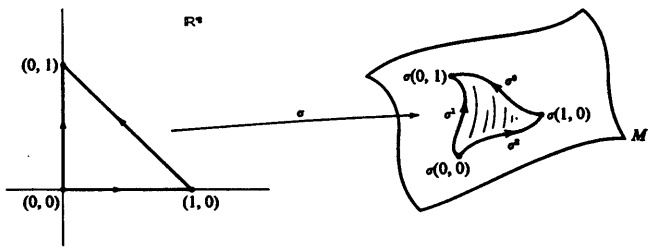
\includegraphics[width=0.60\textwidth]{figures/ch4_img_in_image_box_125_823_775_1072.jpg}
\end{center}

We claim that

\begin{equation}
\label{eq:4.6:5}
k_{i}^{p+1}\circ k_{j}^{p}=k_{j+1}^{p+1}\circ k_{i}^{p}\qquad(p\geq0;i\leq j).
\end{equation}

For $p=0$, check the three possible cases separately. For $p\geq1$, observe that both sides of (5) give the following maps:

\begin{equation}
\label{eq:4.6:6}
\begin{aligned}{}&{{}\quad1\leq i<j\quad(a_{1},\ldots,a_{p})\mapsto(a_{1},\ldots,a_{i-1},0,a_{i},\ldots,a_{j-1},0,a_{j},\ldots,a_{p})}\\ {}&{{}\quad1\leq i=j\quad(a_{1},\ldots,a_{p})\mapsto(a_{1},\ldots,a_{i-1},0,0,a_{i},\ldots,a_{p})}\\ {}&{{}\quad0=i<j\quad(a_{1},\ldots,a_{p})\mapsto\bigg(1-\sum_{i=1}^{p}a_{i},a_{1},\ldots,a_{j-1},0,a_{j},\ldots,a_{p}\bigg)}\\ {}&{{}\quad0=i=j\quad(a_{1},\ldots,a_{p})\mapsto\bigg(0,1-\sum_{i=1}^{p}a_{i},a_{1},\ldots,a_{p}\bigg).}\\ \end{aligned}
\end{equation}

It follows from (5), (3), and (4) that the boundary of the boundary of a chain is always 0. That is,

\begin{equation}
\label{eq:4.6:7}
\partial\circ\partial=0.
\end{equation}

Now let $\sigma$ be a $p$-simplex in $M$, and let $\omega$ be a $p$-form defined on a neighborhood of the image of $\sigma$. In most of our applications we shall deal only with smooth forms, but for the purposes of the following definition it would be quite sufficient for $\omega$ to be a continuous $p$-form. First of all, if $p = 0$, then a 0-simplex consists simply of a point in $M$, and a 0-form is simply a function. In this case, we define the integral of the function $\omega$ over the 0-simplex $\sigma$ to be the value of $\omega$ at the point $\sigma(0) \in M$:

\begin{equation}
\label{eq:4.6:8}
\int_{\sigma}\omega=\omega\left(\sigma(0)\right).
\end{equation}

If $p \geq 1$, then since $\sigma$ extends to be a smooth map of a neighborhood of $\Delta^p$ in $\mathbb{R}^p$ into $M$, $\omega$ can be pulled back via $\sigma$ to a $p$-form $\delta\sigma(\omega)$ on a neighborhood of $\Delta^p$. In this case, we define the integral of the $p$-form $\omega$ over the $p$-simplex $\sigma$ by

\begin{equation}
\label{eq:4.6:9}
\int_{\sigma}\omega=\int_{\Delta^{p}}\delta\sigma(\omega).
\end{equation}

We extend these integrals linearly to chains, so that if  $ c = \sum a_i \sigma_i $, then

\begin{equation}
\label{eq:4.6:10}
\int_{c}\omega=\sum a_{i}\int_{\sigma_{i}}\omega.
\end{equation}

Perhaps the single most important theorem in integration theory on manifolds is Stokes' theorem. This is a generalization of the Fundamental Theorem of Calculus. Observe that in our context the Fundamental Theorem says that if $F$ is a smooth function on the real line, and if $\sigma$ is a smooth 1-simplex in the real line, then

\begin{equation}
\label{eq:4.6:11}
\int_{\partial\sigma}F=\int_{\sigma}dF.
\end{equation}

We shall present two versions of Stokes' theorem. The first is in terms of integration of forms over chains. \index{Stokes' theorem}

\begin{theorem}{Stokes' Theorem I}\label{thm:4.7}
Let $c$ be a $p$-chain ($p \geq 1$) in a differentiable manifold $M$, and let $\omega$ be a smooth ($p-1$) form defined on a neighborhood of the image of $c$. Then

\begin{equation}
\label{eq:4.7:1}
\int_{\partial c}\omega=\int_{c}d\omega.
\end{equation}

\end{theorem}

\begin{proof}
It is sufficient to consider the case in which the p-chain c consists of a single p-simplex  $ \sigma $. Thus we must prove that

\begin{equation}
\label{eq:4.7:2}
\int_{\sigma}d\omega=\int_{\partial\sigma}\omega.
\end{equation}

It follows immediately from our definitions that (2) is equivalent with

\begin{equation}
\label{eq:4.7:3}
\int_{\Delta^{p}}d\left(\delta\sigma(\omega)\right)=\sum_{i=0}^{p}(-1)^{i}\int_{\Delta^{p-1}}\delta\sigma^{i}(\omega)=\sum_{i=0}^{p}(-1)^{i}\int_{\Delta^{p-1}}\delta k_{i}^{p-1}\circ\delta\sigma(\omega).
\end{equation}

Observe first of all that the case p = 1 reduces directly to the Fundamental Theorem of Calculus:

\begin{equation}
\label{eq:4.7:4}
\int_{\Delta^{1}}\frac{d}{d r}(\omega\circ\sigma)d r=\omega\big(\sigma(1)\big)-\omega\big(\sigma(0)\big),
\end{equation}

so we now assume that  $ p \geq 2 $. Then the  $ (p - 1) $ form  $ \delta\sigma(\omega) $ can be expressed as

\begin{equation}
\label{eq:4.7:5}
\delta\sigma(\omega)=\sum_{j=1}^{p}a_{j}\,dr_{1}\wedge\cdots\wedge\widehat{dr_{j}}\wedge\cdots\wedge dr_{p},
\end{equation}

where the circumflex over a term means that the term is to be omitted, and where the $a_i$ are $C^\infty$ functions on a neighborhood of $\Delta^p$ in $\mathbb{R}^p$. Since the integral is linear, we may consider the special case in which $\delta\sigma(\omega)$ consists of a single term of the form $a_i dr_1 \wedge \cdots \wedge \widehat{dr}_j \wedge \cdots \wedge dr_p$. In this case, the left-hand side of (3) becomes

\begin{equation}
\label{eq:4.7:6}
(-1)^{j-1}\int_{\Delta^{p}}\frac{\partial a_{j}}{\partial r_{j}}d r_{1}\wedge\cdots\wedge d r_{p}.
\end{equation}

To evaluate the right-hand side of (3), we observe that for  $ 1 \leq i \leq p $,

\begin{equation}
\label{eq:4.7:7}
\delta k_{i}^{p-1}(r_{j})=\left\{\begin{matrix}{r_{j}}&{}&{(1\leq j\leq i-1)}\\ {0}&{}&{(j=i)}\\ {r_{j-1}}&{}&{(i+1\leq j\leq p),}\\ \end{matrix}\right.
\end{equation}

and

\begin{equation}
\label{eq:4.7:8}
\delta k_{0}^{p-1}(r_{j})=\left\{\begin{aligned}{}&{{}1-\sum_{i=1}^{p-1}r_{i}}&{(j=1)}\\ {}&{{}r_{j-1}}&{(1<j\leq p).}\\ \end{aligned}\right.
\end{equation}

Applying (7) and (8) to the right-hand term of (3), we obtain


\begin{align*}\sum_{i=0}^{p}(-1)^{i}&\int_{\Delta^{p-1}}\delta k_{i}^{p-1}(a_{j} dr_{1}\wedge\cdots\wedge\widehat{dr}_{j}\wedge\cdots\wedge dr_{p})\\&=(-1)^{j-1}\int_{\Delta^{p-1}}a_{j}\bigg(1-\sum_{i=1}^{p-1}r_{i},r_{1},\ldots,r_{p-1}\bigg)dr_{1}\wedge\cdots\wedge dr_{p-1}\\&\quad+(-1)^{j}\int_{\Delta^{p-1}}a_{j}(r_{1},\ldots,r_{j-1},0,r_{j},\ldots,r_{p-1})dr_{1}\wedge\cdots\wedge dr_{p-1}.\end{align*}


We shall now apply a change of variables to the first term on the right-hand side of (9). Let $\varphi_{j}$ be the diffeomorphism of $\mathbb{R}^{p-1}$ defined by

\[
\varphi_{j}(r_{1},\ldots,r_{p-1})=\begin{cases}{(r_{1},\ldots,r_{p-1})}&{(j=1)}\\ {\left(1-\displaystyle\sum_{i=1}^{p-1}r_{i},r_{2},\ldots,r_{p-1}\right)}&{(j=2)}\\ {\left(r_{2},\ldots,r_{j-1},1-\displaystyle\sum_{i=1}^{p-1}r_{i},r_{j},\ldots,r_{p-1}\right)}&{}\\ {\quad(3\leq j\leq p).}\\ \end{cases}
\]

Then  $\varphi_j(\Delta^{p-1}) = \Delta^{p-1}$, and $|J_{\varphi_j}| = 1$, so that by \eqref{eq:4.4:1}, the first term on the right-hand side of (9) is equal to

\[
(-1)^{i-1}\int_{\Delta^{p-1}}a_{j}\left(r_{1},\ldots,r_{j-1},1-\sum_{i=1}^{p-1}r_{i},r_{j},\ldots,r_{p-1}\right)d r_{1}\wedge\cdots\wedge d r_{p-1}.
\]

From (3), (6), (9), and (11) we see that the proof has been reduced to showing that

\begin{equation}
\label{eq:4.7:9}
\begin{aligned}{}&{{}\int_{\Delta^{p}}\frac{\partial a_{j}}{\partial r_{j}}d r_{1}\wedge\cdots\wedge d r_{p}}\\ {}&{{}\quad=\int_{\Delta^{p-1}}a_{j}\bigg(r_{1},\ldots,r_{j-1},1-\sum_{i=1}^{p-1}r_{i},r_{j},\ldots,r_{p-1}\bigg)d r_{1}\wedge\cdots\wedge d r_{p-1}}\\ {}&{{}\quad-\int_{\Delta^{p-1}}a_{j}(r_{1},\ldots,r_{j-1},0,r_{j},\ldots,r_{p-1})d r_{1}\wedge\cdots\wedge d r_{p-1}.}\\ \end{aligned}
\end{equation}

But now (12) is simply the evaluation of the integral of $\partial a_{i}/\partial r_{i}$ over $\Delta^{p}$ by iterating first with respect to $r_{i}$ and applying again the Fundamental Theorem of Calculus.

\end{proof}

\subsection{Integration on an Oriented Manifold}\label{thm:4.8}
Let $M$ be an $n$-dimensional oriented manifold. We shall integrate $n$-forms over regular domains in $M$. A subset $D$ of $M$ will be called a regular domain if for each point $m \in M$ one of the following holds: \index{Regular domain}

(a) There is an open neighborhood of m which is contained in M - D.

(b) There is an open neighborhood of m which is contained in D.

(c) There is a centered coordinate system $(U,\varphi)$ about $m$ such that $\varphi(U\cap D)=\varphi(U)\cap H^n$, where $H^n$ is the half-space of $\mathbb{R}^n$ defined by $r_n\geq0$.

Points of $D$ of type (b) are called interior points and comprise the interior, Int(D), of $D$. Points of type (c) are called boundary points and comprise the boundary, $\partial D$, of $D$. Coordinate systems of type (c) restricted to $\partial D$ overlap differentiably and yield a manifold structure of dimension $n-1$ on $\partial D$, making $\partial D$ into an imbedded $(n-1)$ dimensional submanifold of $M$.

Let $m \in \partial D$, and let $v \in M_m$. We call $v$ an outer vector to $D$ if there is a smooth curve $\alpha(t)$ in $M$ with $\dot{\alpha}(0) = v$ and with $\alpha(t) \notin D$ for $0 < t < \varepsilon$, for some $\varepsilon > 0$. The orientation on $M$ induces an orientation on $\partial D$ as follows. Let $v$ be an outer vector to $D$ at $m$, and let $v_1, \ldots, v_{n-1}$ be a basis of the tangent space $(\partial D)_m$. Then we define $v_1, \ldots, v_{n-1}$ to be an oriented basis of $(\partial D)_m$ if and only if $v, v_1, \ldots, v_{n-1}$ is an oriented basis of $M_m$. One can easily check that this definition is independent of the outer vector $v$ chosen, and that this defines a smooth orientation on $\partial D$ in the sense of 4.1.

Now let $\omega$ be an $n$-form ($n = \dim M$) with compact support, and let $D$ be a regular domain in $M$. As a particular case, $D$ could be all of $M$. We are going to define the integral of $\omega$ over $D$. As in 4.6, it will be sufficient for the purposes of this definition for $\omega$ to be a continuous $n$-form. We shall use a partition of unity to reduce the support of $\omega$ to certain $n$-simplices in $M$ over which we can integrate as in \eqref{eq:4.6:9}. First, we shall choose some $n$-simplices suitably related to $D$ and $\partial D$.

An $n$-simplex $\sigma$ in $M$ will be called regular if $\sigma$ extends to a diffeomorphism on a neighborhood of $\Delta^n$. When speaking of regular $n$-simplices, we shall always assume that they have been extended in this way to a neighborhood of $\Delta^n$. An oriented regular $n$-simplex is one in which the map $\sigma$ preserves orientations. (We always take the standard orientation on $\mathbb{R}^n$.)

Associated with a given regular domain $D$, we shall consider only oriented regular $n$-simplices of the following two types:

$ (\alpha) $  $ \sigma(\Delta^n) \subset \operatorname{Int}(D) $.

$ (\beta) $  $ \sigma(\Delta^n) \subset D $ and  $ \sigma(\Delta^n) \cap \partial D = \sigma^n (\Delta^{n-1}) $; that is, precisely the nth face of  $ \sigma $ lies in the boundary of  $ D $.

Now cover D by open sets U of the following types:

$ (\alpha') \quad U $ lies in the interior of an oriented regular  $ n $-simplex  $ \sigma $ of type  $ (\alpha) $.

$ (\beta') $ U is the image under a type  $ (\beta) $ oriented regular  $ n $-simplex  $ \sigma $ of an open set  $ V $ in  $ \mathbb{R}^n $ which is a neighborhood of a point in the  $ n $th face of  $ \Delta^n $, which intersects the boundary of  $ \Delta^n $ only in that  $ n $th face, and whose image under  $ \sigma $ is contained in  $ \sigma(\Delta^n) \cup (M - D) $.

\begin{center}
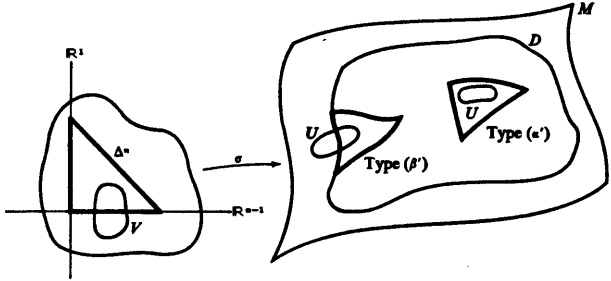
\includegraphics[width=0.60\textwidth]{figures/ch4_img_in_image_box_158_107_769_388.jpg}
\end{center}

Since supp $\omega \cap D$ is compact, it has a finite cover $U_1, \ldots, U_k$ by open sets of type $(\alpha')$ or $(\beta')$. Let the associated oriented regular $n$-simplices be $\sigma_1, \ldots, \sigma_k$. Let $U = M - (\text{supp} \omega \cap D)$, and let $\varphi, \varphi_1, \ldots, \varphi_k$ be a partition of unity subordinate to the cover $U, U_1, \ldots, U_k$ of $M$. We define the integral of $\omega$ over $D$ by

\begin{equation}
\label{eq:4.8:1}
\int_{D}\omega=\sum_{i=1}^{k}\int_{\sigma_{i}}\varphi_{i}\omega.
\end{equation}

We must check that the definition (1) is independent of the cover and the partition of unity chosen. Let $V, V_{1}, \ldots, V_{l}$ and $\psi, \psi_{1}, \ldots, \psi_{l}$ be another such cover and another such partition of unity respectively, with $V_{j}$ associated with the oriented regular $n$-simplex $\tau_{j}$. Since $\psi = 0$ on $\mathrm{supp} \omega \cap D$, it follows that $\sum_{j=1}^{l}\psi_{j} = 1$ there, so that

\begin{equation}
\label{eq:4.8:2}
\sum_{i=1}^{k}\int_{\sigma_{i}}\varphi_{i}\omega=\sum_{i=1}^{k}\int_{\sigma_{i}}\sum_{j=1}^{l}\psi_{j}\varphi_{i}\omega=\sum_{i,j}\int_{\sigma_{i}}\psi_{j}\varphi_{i}\omega.
\end{equation}

Similarly,

\begin{equation}
\label{eq:4.8:3}
\sum_{j=1}^{l}\int_{\tau_{j}}\psi_{j}\omega=\sum_{i,j}\int_{\tau_{j}}\psi_{j}\varphi_{i}\omega.
\end{equation}

Now, since $\sigma_i^{-1}\circ\tau_j$ is an orientation-preserving diffeomorphism on the open set (possibly empty) where it is defined, and since (supp $\psi_j\varphi_i\omega$) $\cap\sigma_i(\Delta^n) = (\mathrm{supp}\,\psi_j\varphi_i\omega)\cap\tau_j(\Delta^n)$, it follows from the change of variables formula \eqref{eq:4.5:2} that

\begin{equation}
\label{eq:4.8:4}
\begin{aligned}{\int_{\sigma_{i}}\psi_{j}\varphi_{i}\omega=}&{{}\int_{\Delta^{n}}\delta\sigma_{i}(\psi_{j}\varphi_{i}\omega)=\int_{\Delta^{n}}\delta(\sigma_{i}^{-1}\circ\tau_{j})[\delta\sigma_{i}(\psi_{j}\varphi_{i}\omega)]}\\ {=}&{{}\int_{\Delta^{n}}\delta\tau_{j}(\psi_{j}\varphi_{i}\omega)=\int_{\tau_{j}}\psi_{j}\varphi_{i}\omega.}\\ \end{aligned}
\end{equation}

It follows from (2), (3), and (4) that $\int_{D} \omega$ is well-defined, independent of the choice of cover and partition of unity.

Observe that if $\gamma$ is a diffeomorphism of $M$, then

\begin{equation}
\label{eq:4.8:5}
\int_{\gamma(D)}\omega=\pm\int_{D}\delta\gamma(\omega)
\end{equation}

with “+” if and only if  $ \gamma $ is orientation-preserving.

We now are ready to state and prove our second version of Stokes' theorem.

\begin{theorem}{Stokes' Theorem II}\label{thm:4.9}
Let $D$ be a regular domain in an oriented $n$-dimensional manifold $M$, and let $\omega$ be a smooth $(n-1)$ form of compact support. Then

\begin{equation}
\label{eq:4.9:1}
\int_{D}d\omega=\int_{\partial D}\omega.
\end{equation}

\end{theorem}

\begin{proof}
Let $\varphi_{1},\ldots,\varphi_{k}$ and $\sigma_{1},\ldots,\sigma_{k}$ be chosen as in \eqref{eq:4.8:1} relative to (supp $\omega$) $\cap D$. Since $\sum_{i=1}^{k}\varphi_{i}=1$ on a neighborhood of (supp $\omega$) $\cap D$, $d(\sum\varphi_{i})=0$ there. Thus on a neighborhood of (supp $\omega$) $\cap D$ we have

\begin{equation}
\label{eq:4.9:2}
\sum_{i=1}^{k}d(\varphi_{i}\omega)=\sum_{i=1}^{k}d\varphi_{i}\wedge\omega+\sum_{i=1}^{k}\varphi_{i}d\omega=d\omega.
\end{equation}

Now, if $\sigma_{i}$ is an $n$-simplex of type 4.8( $ \alpha $), then

\begin{equation}
\label{eq:4.9:3}
\int_{\partial\sigma_{i}}\varphi_{i}\omega=0=\int_{\partial D}\varphi_{i}\omega
\end{equation}

since $\mathrm{supp} \ \varphi_i \omega \subset \mathrm{Int} \ \sigma_i(\Delta^n) \subset \mathrm{Int} \, D$. On the other hand, suppose that $\sigma_i$ is an $n$-simplex of type 4.8($\beta$). In this case, $\varphi_i \omega$ is zero on the boundary of $\sigma_i$ except possibly at points in the interior of the $n$th face $\sigma_i^n$. Now $\sigma_i^n$ is an orientation-preserving regular ($n-1$) simplex in $\partial D$ if $n$ is even, and is orientation-reversing if $n$ is odd. It follows that

\begin{equation}
\label{eq:4.9:4}
\int_{\partial\sigma_{i}}\varphi_{i}\omega=(-1)^{n}\int_{\sigma_{i}{}^{n}}\varphi_{i}\omega=(-1)^{n}(-1)^{n}\int_{\partial D}\varphi_{i}\omega=\int_{\partial D}\varphi_{i}\omega.
\end{equation}

From (2), (3), (4), and from our first version (4.7) of Stokes' theorem, we see that

\begin{equation}
\label{eq:4.9:5}
\begin{aligned}{\int_{D}d\omega}&{{}=\sum_{i}\int_{D}d(\varphi_{i}\omega)=\sum_{i}\int_{\sigma_{i}}d(\varphi_{i}\omega)}\\ {}&{{}=\sum_{i}\int_{\partial\sigma_{i}}\varphi_{i}\omega=\sum_{i}\int_{\partial D}\varphi_{i}\omega=\int_{\partial D}\omega.}\\ \end{aligned}
\end{equation}

\end{proof}

\begin{corollary*}
Let $\omega$ be a smooth $(n-1)$ form on a compact oriented $n$-dimensional manifold $M$. Then

\[
\int_M d\omega=0.
\]

\end{corollary*}

\subsection{Integration on a Riemannian Manifold}\label{thm:4.10} Let $M$ be a Riemannian manifold of dimension $n$. That is, $M$ is an $n$-dimensional differentiable manifold with a positive definite inner product $\langle \ , \rangle_m$ on each tangent space $M_m$ such that $m \mapsto \langle X, Y \rangle_m$ is a smooth function on $M$ whenever $X$ and $Y$ are smooth vector fields. The existence of Riemannian metrics on differentiable manifolds was asserted in Exercise 23 of Chapter 1.

Given a point  $ m \in M $, one can find a neighborhood  $ U $ of  $ m $ and a collection  $ e_1, \ldots, e_n $ of  $ C^\infty $ vector fields on  $ U $ which are orthonormal in the sense that they form an orthonormal basis of the tangent space to  $ M $ at each point of  $ U $. Start with a coordinate neighborhood  $ (U, x_1, \ldots, x_n) $, apply the usual Gram-Schmidt procedure to orthonormalize the vector fields  $ \partial/\partial x_1, \ldots, \partial/\partial x_n $, and do it simultaneously at all points of  $ U $. Such a collection  $ e_1, \ldots, e_n $ is called a local orthonormal frame field. \index{Frame field}

Since the inner product  $ \langle \quad, \quad\rangle_{m} $ is, in particular, a non-singular pairing of  $ M_{m} $ with itself, it induces (see 2.7) a natural isomorphism of  $ M_{m} $ with  $ M_{m}^{*} $, namely,  $ v \mapsto \varphi_{v} $ where

\begin{equation}
\label{eq:4.10:1}
\varphi_{v}(w)=\langle v,w\rangle_{m}.
\end{equation}

Via this isomorphism,  $ M_{m}^{*} $ inherits an inner product. Observe that the dual basis to an orthonormal basis of  $ M_{m} $ is itself an orthonormal basis for  $ M_{m}^{*} $.

Now let  $ e_{1}, \ldots, e_{n} $ be a local orthonormal frame field on U, and let  $ \omega_{1}, \ldots, \omega_{n} $ be the dual 1-forms. That is,

\begin{equation}
\label{eq:4.10:2}
\omega_{i}(e_{j})=\delta_{ij}\quad\mathrm{on}~U.
\end{equation}

Then $\omega_{1}, \ldots, \omega_{n}$ form a local orthonormal coframe field on $U$. Consider now two local orthonormal coframe fields $\omega_{1}, \ldots, \omega_{n}$ on $U$ and $\omega_{1}^{\prime}, \ldots, \omega_{n}^{\prime}$ on $U^{\prime}$. Then on $U \cap U^{\prime}$ \index{Coframe field}

\begin{equation}
\label{eq:4.10:3}
\omega_{1}\wedge\cdots\wedge\omega_{n}=\det(\sigma)\,\omega_{1}^{\prime}\wedge\cdots\wedge\omega_{n}^{\prime}
\end{equation}

where  $ \sigma $ is an orthogonal matrix whose entries are  $ C^{\infty} $ functions on  $ U \cap U' $. Thus

\begin{equation}
\label{eq:4.10:4}
\omega_{1}\wedge\cdots\wedge\omega_{n}=\pm\omega_{1}^{\prime}\wedge\cdots\wedge\omega_{n}^{\prime}.
\end{equation}

Now assume that $M$ is oriented. A local coframe field $\omega_1, \ldots, \omega_n$ on $U$ will be called oriented if $\omega_1 \wedge \cdots \wedge \omega_n$ belongs to the orientation at each point of $U$. Choose a local oriented orthonormal coframe field about each point of $M$. Then the corresponding $n$-forms $\omega_1 \wedge \cdots \wedge \omega_n$ agree on overlaps, and therefore determine a globally defined nowhere-vanishing $n$-form $\omega$ on $M$. This form $\omega$ is called the volume form of the oriented Riemannian manifold $M$. Its integral over $M$ is the volume of $M$. \index{Volume}\index{Volume form}

In Exercise 13 of Chapter 2, the star operator * was introduced on $\Lambda(V)$ for an oriented inner product space $V$. On an oriented Riemannian manifold $M$, we therefore have * defined on $\Lambda(M_{m}^{*})$ for each $m$. It is easy to see that * takes smooth forms to smooth forms, so we have a linear operator

\begin{equation}
\label{eq:4.10:5}
*:E^{p}(M)\to E^{n-p}(M),
\end{equation}

which, according to Exercise 13 of Chapter 2, satisfies

\begin{equation}
\label{eq:4.10:6}
**=(-1)^{p(n-p)}.
\end{equation}

We already know from 4.8 how to integrate $n$-forms over an oriented $n$-dimensional manifold. Now in the case of an oriented Riemannian manifold $M$, we define the integral over $M$ of a continuous function $f$ with compact support to be the integral of the (continuous) $n$-form $*f = f_\omega$. That is,

\begin{equation}
\label{eq:4.10:7}
\int_{M}f=\int_{M}*f=\int_{M}f\omega.
\end{equation}

Actually, the orientation was convenient but not necessary in the definition of $\int_{M} f$. If $M$ is a (not necessarily oriented) Riemannian manifold, we define the integral of continuous functions with compact support as follows. Let $\{U_\alpha\}$ be a cover of $M$ by interiors of regular $n$-simplices $\sigma_\alpha$, and let $\omega_1^\alpha, \ldots, \omega_n^\alpha$ be a local orthonormal coframe field defined on a neighborhood of $\sigma_\alpha(\Delta^n)$. Then there exist $C^\infty$ functions $h_\alpha$ on neighborhoods of $\Delta^n$ such that

\[
\delta\sigma_{\alpha}(\omega_{1}^{\alpha}\wedge\cdots\wedge\omega_{n}^{\alpha})=h_{\alpha}\,dr_{1}\wedge\cdots\wedge dr_{n}.
\]

Let $\{\varphi_{\alpha}\}$ be a partition of unity subordinate to the cover $\{U_{\alpha}\}$, and let $f$ be a continuous function with compact support on $M$. Then we define

\begin{equation}
\label{eq:4.10:8}
\int_{M}f=\sum_{\alpha}\int_{\Delta^{n}}(\varphi_{\alpha}f)\circ\sigma_{\alpha}\left|h_{\alpha}\right|d r_{1}\wedge\cdots\wedge d r_{n}.
\end{equation}

That this definition is independent of the cover and partition of unity chosen follows from an argument similar to the one at the end of 4.8. In the case of an oriented Riemannian manifold, (8) and (7) agree.

In classical vector analysis the gradient of a function $f$ on $\mathbb{R}^n$ is defined to be the vector field $\sum_{i=1}^{n}(\partial f/\partial r_i)\partial/\partial r_i$, and the divergence of a vector field $V=\sum_{i=1}^{n}v_i\,\partial/\partial r_i$ is defined to be the function $\sum_{i=1}^{n}\partial v_i/\partial r_i$. We extend these notions to general Riemannian manifolds as follows. Recall that the metric gives us canonical isomorphisms $M_m\cong M_m^*$. We shall for convenience denote such isomorphisms by a tilde, so that if $v\in M_m$, then $\tilde{v}$ will be the corresponding dual element in $M_m^*$; and if $\omega\in M_m^*$, then $\tilde{\omega}$ will be the corresponding vector in $M_m$. Then if $f$ is a function on $M$, its gradient is the vector field \index{Divergence of a vector field}\index{Gradient}

\begin{equation}
\label{eq:4.10:9}
\mathrm{grad}f=\widetilde{df}.
\end{equation}

If V is a vector field on an oriented Riemannian manifold, then its divergence is the function

\begin{equation}
\label{eq:4.10:10}
\mathrm{div}\,V=*d*\tilde{V}.
\end{equation}

Stokes' theorem has an equivalent version on oriented Riemannian manifolds known as the divergence theorem. This theorem says that if $V$ is a smooth vector field on an oriented Riemannian manifold $M$, if $D$ is a regular domain in $M$, and if $\vec{n}$ is the unit outer normal vector field on $\partial D$, then \index{Divergence theorem}

\begin{equation}
\label{eq:4.10:11}
\int_{D}\mathrm{div}\,V=\int_{\partial D}\langle V,\vec{n}\rangle.
\end{equation}

The proof is left to the reader as an exercise. (For a few additional remarks see Exercise 4.)

\subsection{Integration on a Lie Group}\label{thm:4.11}
Let $G$ be an $n$-dimensional Lie group. We observed in \hyperref[thm:4.3]{4.3(a)} that G is orientable. We now fix once and for all an orientation on G.

Consider the left invariant $n$-forms on $G$. Since such a form is uniquely determined by its value at one point, and since the $n$th exterior power of an $n$-dimensional vector space is one-dimensional, there is exactly a one-dimensional space of left invariant $n$-forms on $G$. Choose a non-zero left invariant $n$-form $\omega$ consistent with the fixed orientation on $G$.

Since $G$ is oriented, the integral of compactly supported $n$-forms is defined on $G$ as in 4.8. We now define, with respect to $\omega$, the integral of a compactly supported continuous function $f$ on $G$ by setting

\begin{equation}
\label{eq:4.11:1}
\int_{G}f=\int_{G}f\omega.
\end{equation}

The integral (1) depends, of course, on the choice of the non-zero left invariant n-form  $ \omega $ consistent with the orientation on G. But since such forms are uniquely determined up to a positive constant multiple, so is the integral (1). In the case of a compact group G, we can and always will fix the choice of  $ \omega $ by requiring the normalization

\begin{equation}
\label{eq:4.11:2}
\int_{G}\omega=1.
\end{equation}

Consider the diffeomorphism $l_{\sigma}$, which is left translation by the element $\sigma$ of $G$. Then since $\delta l_{\sigma}(\omega) = \omega$, $l_{\sigma}$ is orientation-preserving, so that, according to \eqref{eq:4.8:5},

\begin{equation}
\label{eq:4.11:3}
\int_{G}f=\int_{G}f\omega=\int_{G}\delta l_{\sigma}(f\omega)=\int_{G}(f\circ l_{\sigma})\omega=\int_{G}f\circ l_{\sigma}.
\end{equation}

In view of property (3)—that the integral of a function $f$ on $G$ is the same as the integral of any of its left translates $f\circ l_\sigma$—we call the integral (1) left invariant.

Now we ask to what extent the integral (1) is also right invariant. That is, when do we have

\begin{equation}
\label{eq:4.11:4}
\int_{G}f=\int_{G}f\circ r_{\sigma}
\end{equation}

for each $\sigma \in G$? The form $\delta r_{\sigma}\omega$ is still left invariant, since

\[
\delta l_{\tau}\delta r_{\sigma}\omega=\delta r_{\sigma}\delta l_{\tau}\omega=\delta r_{\sigma}\omega.
\]

Thus $\delta r_{\sigma}\omega$ is some constant multiple of $\omega$. Thus there is defined a function $\tilde{\lambda}$ of $G$ into the non-zero real numbers such that

\begin{equation}
\label{eq:4.11:5}
\delta r_{\sigma}(\omega)=\tilde{\lambda}(\sigma)\omega.
\end{equation}

It is easily checked that  $ \tilde{\lambda} $ is  $ C^{\infty} $. We let

\begin{equation}
\label{eq:4.11:6}
\lambda(\sigma)=|\tilde{\lambda}(\sigma)|.
\end{equation}

Observe that

\begin{equation}
\label{eq:4.11:7}
\lambda(\sigma\tau)=\lambda(\sigma)\lambda(\tau),
\end{equation}

so that $\lambda$ is a Lie group homomorphism of $G$ into the multiplicative group of positive real numbers. $\lambda$ is called the modular function. Now since, by \eqref{eq:4.8:5}, for each $\sigma$ in $G$ \index{Modular function}

\[
\int_{G}f\omega=\int_{G}(f\circ r_{\sigma})\lambda(\sigma)\omega,
\]

it follows that the integral (1) is right invariant if and only if $\lambda \equiv 1$ on $G$. A Lie group $G$ for which $\lambda \equiv 1$ is called unimodular. We observe that each compact Lie group $G$ is unimodular since for each $\sigma \in G$

\[
1=\int_{G}\omega=\lambda(\sigma)\int_{G}\omega=\lambda(\sigma).
\]

Thus the integral on a compact Lie group is both left and right invariant.

\subsection{Application of 4.11}\label{thm:4.12}
A typical application of the integral on a compact Lie group is the following.

Let $G$ be a Lie group, and let $\alpha: G \to \mathrm{Aut}(V)$ be a representation into the automorphisms of a real or complex inner product space $V$. The representation $\alpha$ is called unitary (respectively orthogonal) in the case in which $V$ is a complex (respectively real) inner product space if

\begin{equation}
\label{eq:4.12:1}
\langle\alpha(\tau)v,\alpha(\tau)w\rangle=\langle v,w\rangle
\end{equation}

for all v and w in V and for all  $ \tau \in G $.

Let $G$ be compact and $V$ complex (respectively real). Then there is an inner product on $V$ with respect to which $\alpha$ is unitary (respectively orthogonal). The proofs in the real case and in the complex cases are similar. Let \{, \} be any inner product on $V$. We set

\begin{equation}
\label{eq:4.12:2}
\langle v,w\rangle=\int_{G}\{\alpha(\sigma)v,\alpha(\sigma)w\}d\sigma,
\end{equation}

where we use $d\sigma$ to denote that we are considering the integrand as a function of $\sigma$ in $G$. It is immediate that $\langle\quad,\quad\rangle$ is again an inner product. That (1) holds follows from the right invariance of the integral on $G$:


\begin{align*}\langle\alpha(\tau)v,\alpha(\tau)w\rangle=&\int_{G}\left\{\alpha(\sigma)\alpha(\tau)v,\alpha(\sigma)\alpha(\tau)w\right\}d\sigma\\=&\int_{G}\left\{\alpha(\sigma\tau)v,\alpha(\sigma\tau)w\right\}d\sigma=\int_{G}\left\{\alpha(\sigma)v,\alpha(\sigma)w\right\}d\sigma=\langle v,w\rangle.\end{align*}


\section{De Rham Cohomology}


\begin{definition}\label{thm:4.13}
A p-form $\alpha$ on a differentiable manifold $M$ is called closed if $d\alpha = 0$. It is called exact if there is a $(p - 1)$ form $\beta$ such that $\alpha = d\beta$. Since $d^{2} = 0$, every exact form is closed. The quotient space of the real vector space of closed $p$-forms modulo the subspace of exact $p$-forms is called the $p$th \emph{de Rham cohomology group of $M$}. \index{de Rham cohomology}

\begin{equation}
\label{eq:4.13:1}
H_{\mathrm{de\,R}}^{p}(M)=\{\mathrm{closed}~p\mathrm{-forms}\}/\{\mathrm{exact}~p\mathrm{-forms}\}.
\end{equation}

\end{definition}

\begin{examples}\label{thm:4.14}
Consider the case of the unit circle  $ S^1 $. Since there are no non-zero p-forms on  $ S^1 $ for  $ p > 1 $, all of the cohomology groups  $ H_{\mathrm{de\,R}}^{p}(S^{1}) $ are zero except possibly for  $ p = 0, 1 $. There are no exact 0-forms, and a closed 0-form on a connected manifold is simply a constant function, so

\begin{equation}
\label{eq:4.14:1}
H_{\mathrm{de\,R}}^{0}(S^{1})\cong\mathbb{R}.
\end{equation}

The “polar coordinate function” $\theta$ on $S^1$ is not well-defined globally since it is defined only up to integral multiples of $2\pi$. However, its differential $d\theta$ is a globally well-defined nowhere-vanishing 1-form on $S^1$. In fact, $d\theta$ is the volume form of the natural Riemannian metric which $S^1$ inherits from $\mathbb{R}^2$. Now, $d\theta$ is not exact, for if it were, its integral over $S^1$ would have to be 0 rather than $2\pi$. All 1-forms on $S^1$ are closed. We claim that if $\alpha$ is a 1-form, then there is a constant $c$ such that $\alpha - c\,d\theta$ is exact. For let $\alpha = f(\theta)\,d\theta$, let

\[
c=\frac{1}{2\pi}\int_{S^{1}}\alpha,
\]

and let

\[
g(\theta)=\int_{0}^{\theta}\left(f(\theta)-c\right)d\theta.
\]

Since  $ g(\theta + 2\pi n) = g(\theta) $ for every integer n, then g is a well-defined  $ C^\infty $ function on  $ S^1 $; and  $ dg = (f(\theta) - c) d\theta = \alpha - c d\theta $. Thus every 1-form on  $ S^1 $ differs from a real multiple of  $ d\theta $ by an exact form. Consequently,

\begin{equation}
\label{eq:4.14:2}
H_{\mathrm{de\,R}}^{1}(S^{1})\cong\mathbb{R}.
\end{equation}

\end{examples}

\subsection{Effect of Mappings}\label{thm:4.15}
Let $f: M \to N$ be a $C^\infty$ map. Then the algebra homomorphism $\delta f: E^*(N) \to E^*(M)$ commutes with $d$, according to 2.23, and hence maps closed forms to closed forms and exact forms to exact forms. Thus it induces a homomorphism

\begin{equation}
\label{eq:4.15:1}
f^{*}\colon H_{\mathrm{de\,R}}^{p}(N)\to H_{\mathrm{de\,R}}^{p}(M)
\end{equation}

for each integer  $ p \geq 0 $. If, in addition,  $ g: N \to X $ is  $ C^\infty $, then

\begin{equation}
\label{eq:4.15:2}
(g\circ f)^{*}=f^{*}\circ g^{*}.
\end{equation}

Clearly the identity map id: $M \to M$ induces the identity on de Rham cohomology:

\begin{equation}
\label{eq:4.15:3}
(\mathrm{id})^{*}=\mathrm{id}.
\end{equation}

It follows from (2) and (3) that a diffeomorphism $f\colon M\to N$ induces isomorphisms on de Rham cohomology. Thus the de Rham cohomology is a differentiable invariant of a differentiable manifold $M$. We shall prove in Chapter 5 that it is actually a topological invariant. That is, the de Rham cohomology groups depend only on the underlying topological structure of $M$ and do not depend on the differentiable structure. A key part in the proof of this fact is the de Rham theorem, a version of which we shall formulate now. First, we need to define the real differentiable singular homology groups of $M$. \index{Real differentiable singular homology}\index{de Rham theorem}

\subsection{Real Differentiable Singular Homology}\label{thm:4.16}
For each integer $p \geq 0$ we let ${}_{\infty}S_p(M,\mathbb{R})$ denote the real vector space generated by the differentiable singular $p$-simplices in $M$. Hence the elements of ${}_{\infty}S_p(M,\mathbb{R})$ are precisely the differentiable singular $p$-chains in $M$ with real coefficients. For $p < 0$, we let ${}_{\infty}S_p(M,\mathbb{R})$ be the zero vector space. The boundary operator $\partial$ induces linear transformations

\begin{equation}
\label{eq:4.16:1}
\partial_{p}\colon{}_{\infty}S_{p}(M,\mathbb{R})\to{}_{\infty}S_{p-1}(M,\mathbb{R})
\end{equation}

for each integer $p$, which for $p \leq 0$ are simply the zero transformation. According to \eqref{eq:4.6:7}, $\partial_{p} \circ \partial_{p+1} = 0$, so that the image of $\partial_{p+1}$ lies in the kernel of $\partial_{p}$. The $p$th differential singular homology group of $M$ with real coefficients is defined by

\begin{equation}
\label{eq:4.16:2}
{}_{\infty}H_{p}(M;\mathbb{R})=\ker\partial_{p}/\mathrm{Im}\,\partial_{p+1},
\end{equation}

and is moreover a real vector space. Elements of $\ker\partial_{p}$ are called differentiable $p$-cycles, and elements of $\mathrm{Im}\,\partial_{p+1}$ are called differentiable $p$-boundaries.

\subsection{The de Rham Theorem}\label{thm:4.17}
We shall define a linear mapping of the de Rham cohomology  $ H_{\mathrm{de\,R}}^{p}(M) $ into the dual space ${}_{\infty}H_{p}(M;\mathbb{R})^{*}$ of the real differentiable singular homology:

\begin{equation}
\label{eq:4.17:1}
H_{\mathrm{de\,R}}^{p}(M)\to{}_{\infty}H_{p}(M;\mathbb{R})^{*}.
\end{equation}

Let $\alpha$ be a closed $p$-form representing the de Rham cohomology class $\{\alpha\}$, and let $z$ be a $p$-cycle representing the real differentiable singular homology class $\{z\}$. Then (1) is defined by

\begin{equation}
\label{eq:4.17:2}
\{\alpha\}(\{z\})=\int_{z}\alpha.
\end{equation}

That (2) is independent of the representatives  $ \alpha $ and z chosen follows immediately from Stokes' theorem I (4.7).

\emph{The de Rham theorem asserts that (1) is an isomorphism.} This will be proved in 5.36 and 5.37. The real numbers determined by the integrals of a differential form over differentiable cycles are called the periods of the differential form. Now, Stokes' theorem I says that the periods of an exact form are all zero. The injectiveness of the isomorphism (1) gives a converse, namely, if a closed form has all of its periods zero, then it is an exact form. The surjectivity of (1) says that if a real number per(z) is assigned to each cycle z in such a way that

\begin{equation}
\label{eq:4.17:3}
\operatorname{per}(az_{1}+z_{2})=a\operatorname{per}(z_{1})+\operatorname{per}(z_{2}),\qquad\operatorname{per}(\mathrm{boundary})=0,
\end{equation}

then there is a closed form  $ \alpha $ on M such that for all cycles z

\begin{equation}
\label{eq:4.17:4}
\int_{z}\alpha=\operatorname{p e r}(z).
\end{equation}

A key ingredient in the proof of the de Rham theorem (see 5.28) is the

\begin{lemma}{Poincaré Lemma}\label{thm:4.18}
Let $U$ be the open unit ball in Euclidean space  $ \mathbb{R}^n $, and let  $ E^k(U) $, as usual, be the space of differential k-forms on U. Then for each  $ k \geq 1 $ there is a linear transformation  $ h_k: E^k(U) \to E^{k-1}(U) $ such that \index{Poincaré lemma}

\begin{equation}
\label{eq:4.18:1}
h_{k+1}\circ d+d\circ h_{k}=\mathrm{id}.
\end{equation}

\end{lemma}

\begin{proof}
We begin with formula \hyperref[thm:2.25]{2.25(d)}, which expresses the Lie derivative in terms of exterior differentiation and interior multiplication:

\begin{equation}
\label{eq:4.18:2}
L_{X}=i(X)\circ d+d\circ i(X).
\end{equation}

We shall apply (2) to the radial vector field

\begin{equation}
\label{eq:4.18:3}
X=\sum_{i=1}^{n}r_{i}\frac{\partial}{\partial r_{i}}
\end{equation}

on $U$. We define a linear operator $\alpha_{k}$ on $E^{k}(U)$ by setting

\begin{equation}
\label{eq:4.18:4}
\alpha_{k}(f\,dr_{i_{1}}\wedge\cdots\wedge dr_{i_{k}})(p)=\left(\int_{0}^{1}t^{k-1}f(t p)\;d t\right)\;d r_{i_{1}}\wedge\cdots\wedge d r_{i_{k}}(p)
\end{equation}

and extending linearly to all of  $ E^{k}(U) $. Now with X defined by (3), we show that

\begin{equation}
\label{eq:4.18:5}
\alpha_{k}\circ L_{X}=\operatorname{id}\quad\operatorname{on}\quad E^{k}(U).
\end{equation}

For, using the fact that $L_{X}$ is a derivation which commutes with $d$, we have

\begin{equation}
\label{eq:4.18:6}
\begin{aligned}{\alpha_{k}\circ L_{X}(f}&{{}dr_{i_{1}}\wedge\cdots\wedge dr_{i_{k}})(p)}\\ {}&{{}=\alpha_{k}\bigg\{\left(k f+\sum r_{i}\frac{\partial f}{\partial r_{i}}\right)dr_{i_{1}}\wedge\cdots\wedge dr_{i_{k}}\bigg\}(p)}\\ {}&{{}=\left(\int_{0}^{1}t^{k-1}\bigg(k f(t p)+\sum r_{i}(t p)\frac{\partial f}{\partial r_{i}}\bigg|_{t p}\right)d t\bigg)dr_{i_{1}}\wedge\cdots\wedge dr_{i_{k}}(p)}\\ {}&{{}=\left(\int_{0}^{1}\frac{d}{d t}\left(t^{k}f(t p)\right)d t\right)dr_{i_{1}}\wedge\cdots\wedge dr_{i_{k}}(p)}\\ {}&{{}=f(p)dr_{i_{1}}\wedge\cdots\wedge dr_{i_{k}}(p).}\\ \end{aligned}
\end{equation}

From (5) and (2) we obtain

\begin{equation}
\label{eq:4.18:7}
\mathrm{i d}=\alpha_{k}\circ i(X)\circ d+\alpha_{k}\circ d\circ i(X)
\end{equation}

on  $ E^{k}(U) $ with X given by (3). Now  $ \alpha $ commutes with  $ d $; that is,

\[
\alpha_{k}\circ d=d\circ\alpha_{k-1}.
\]

For

\[
\begin{aligned}{\alpha_{k}\circ d(f dr_{i_{1}}\wedge\cdots\wedge dr_{i_{k-1}})(p)}\\ {=}&{{}\alpha_{k}\bigg(\sum\frac{\partial f}{\partial r_{i}}d r_{i}\wedge dr_{i_{1}}\wedge\cdots\wedge dr_{i_{k-1}}\bigg)(p)}\\ {=}&{{}\left(\int_{0}^{1}t^{k-1}\sum\frac{\partial f}{\partial r_{i}}\bigg|_{t p}d t\right)d r_{i}\wedge dr_{i_{1}}\wedge\cdots\wedge dr_{i_{k-1}}(p)}\\ {=}&{{}d\left(\int_{0}^{1}t^{k-2}f(t p)d t\right)dr_{i_{1}}\wedge\cdots\wedge dr_{i_{k-1}}(p)}\\ {=}&{{}d\circ\alpha_{k-1}(f dr_{i_{1}}\wedge\cdots\wedge dr_{i_{k-1}})(p).}\\ \end{aligned}
\]

Thus from (8) and (7) we obtain


\[
\mathrm{i d}=\alpha_{k}\circ i(X)\circ d+d\circ\alpha_{k-1}\circ i(X)
\]

on  $ E^{k}(U) $. Thus the desired linear transformation  $ h_{k} $ which yields (1) is obtained by setting

\[
h_{k}=\alpha_{k-1}\circ i\left(\sum r_{i}\frac{\partial}{\partial r_{i}}\right).
\]

\end{proof}

\begin{corollary*}{a}
If $\omega$ is a $k$-form, $k \geq 1$, on the open unit ball in $\mathbb{R}^n$ and $d\omega = 0$, then there exists a $(k-1)$ form $\beta$ (namely $h_k(\omega)$) such that $d\beta = \omega$.

\end{corollary*}

\begin{corollary*}{b}
The de Rham cohomology groups of the open unit ball in  $ \mathbb{R}^n $ are all zero for  $ p \geq 1 $.
\end{corollary*}

\begin{remarks}\label{thm:4.19}
Let $f_{1}$ and $f_{2}$ be $C^{\infty}$ maps of $M$ into $N$. Then we have induced maps

\begin{equation}
\label{eq:4.19:1}
\delta f_{i}\colon E^{k}(N)\to E^{k}(M)\quad\mathrm{for~each~}k.
\end{equation}

If we wish to prove that $\delta f_{1}$ and $\delta f_{2}$ both induce the same homomorphism on de Rham cohomology, then we need only find a collection of linear transformations

\begin{equation}
\label{eq:4.19:2}
h_{k}\colon E^{k}(N)\to E^{k-1}(M)
\end{equation}

such that

\begin{equation}
\label{eq:4.19:3}
h_{k+1}\circ d+d\circ h_{k}=\delta f_{1}-\delta f_{2}.
\end{equation}

For then, if $\alpha$ is a closed form on $N$, $\delta f_{1}(\alpha)$ and $\delta f_{2}(\alpha)$ differ by an exact form, and thus lie in the same cohomology class. Such a collection of linear transformations $\{h_{k}\}$ is called a homotopy operator for $f_{1}$ and $f_{2}$. In the Poincaré lemma we found a homotopy operator between the identity map of the open unit ball $U$ and any constant map (range 1 point) of $U$ into itself. \index{Homotopy operator}

\end{remarks}

\section{Exercises}

\begin{problemset}

\item Prove the assertion of \hyperref[thm:4.3]{4.3(c)} that a $d$-dimensional manifold $X$ for which there exists an immersion $f: X \to \mathbb{R}^{d+1}$ is orientable if and only if there is a smooth nowhere-vanishing normal vector field along $(X,f)$.

\item Prove that the real projective space $P^{n}$ is orientable if and only if $n$ is odd. (Hint: Observe that the antipodal map on the $n$-sphere $S^{n}$ is orientation-preserving if and only if $n$ is odd.)

\item Carry out in detail the proof of the existence of local orthonormal frame fields on a Riemannian manifold.

\item Prove the divergence \hyperref[thm:4.10]{theorem 4.10}(11). This follows from Stokes' theorem together with the identity

\begin{equation}
\int_{\partial D}\ast\widetilde{V}=\int_{\partial D}\langle V,\vec{n}\rangle.
\end{equation}

The easiest way to see (1) is to choose a local oriented orthonormal frame field  $ e_1, \ldots, e_n $ on a neighborhood of a point of  $ \partial D $, such that at points of  $ \partial D $,  $ e_1 $ is the outer unit normal vector and  $ e_2, \ldots, e_n $ form an oriented basis of the tangent space to  $ \partial D $. Then express  $ *\tilde{V} $ and  $ \langle V,\vec{n} \rangle $ in terms of this local frame field and its dual coframe field  $ \omega_1, \ldots, \omega_n $.

\item Let $M$ be an oriented Riemannian manifold, let $f$ and $g$ be $C^{\infty}$ functions on $M$, and let $D$ be a regular domain in $M$. The Laplacian of $g$, denoted $\Delta g$, is defined by

\begin{equation}
\Delta g=-*d*d g.
\end{equation}

(For more on the Laplacian, see Chapter 6. Observe that our choice of sign for the Laplacian yields $\Delta g = -\sum_{i=1}^{n} \partial^{2} g/\partial r_{i}^{2}$ for $g$ a $C^{\infty}$ function on Euclidean space $\mathbb{R}^{n}$ with its standard Riemannian structure in which $\{\partial/\partial r_{i}\}$ is an orthonormal basis of each tangent space.) If $\vec{n}$ is the unit outer normal vector field along $\partial D$, we let $\partial g/\partial n$ denote $\vec{n}(g)$. Prove the following two Green's identities: \index{Green's identities}

Green's 1st:

\[
\int_{\partial D}f\frac{\partial g}{\partial n}=\int_{D}\langle\mathrm{grad}\,f,\mathrm{grad}\,g\rangle-\int_{D}f\Delta g.
\]

Green's 2nd:

\[
\int_{\partial D}\left(f\frac{\partial g}{\partial n}-g\frac{\partial f}{\partial n}\right)=\int_{D}(g\Delta f-f\Delta g).
\]

\item Let $\omega$ be the volume form of an oriented Riemannian manifold of dimension $n$. Let $X_{1},\ldots,X_{n}$ and $Y_{1},\ldots,Y_{n}$ be vector fields on $M$. Prove that

\[
\omega(X_{1},\ldots,X_{n})\cdot\omega(Y_{1},\ldots,Y_{n})=\det\{\langle X_{i},Y_{j}\rangle\}.
\]

Prove also that

\[
\omega(X_{1},\ldots,X_{n})\omega=\widetilde{X}_{1}\wedge\cdots\wedge\widetilde{X}_{n},
\]

where  $ \tilde{X}_{i} $ is the 1-form dual (via the Riemannian structure) to the vector field  $ X_{i} $.

\item Prove the differentiability of the function $\tilde{\lambda}$ of \eqref{eq:4.11:5}.

\item Let $G$ be a compact (oriented) Lie group, and let $\alpha(\sigma) = \sigma^{-1}$ for $\sigma \in G$. Prove that for every continuous function $f$ on $G$

\[
\int_{G}f=\int_{G}f\circ\alpha.
\]

\item Prove that a Lie group $G$ has a bi-invariant Riemannian metric (that is, a metric such that both $dl_\sigma$ and $dr_\sigma$ preserve the inner products for each $\sigma\in G$) if and only if the closure of $\mathrm{Ad}(G)$ in $\mathrm{Aut}(\mathfrak{g})$ is compact.

\item (a) Prove that  $ H_{\mathrm{de\,R}}^{p}(\mathbb{R}^{n})=0 $ for each  $ p \geq 1 $ and each  $ n \geq 1 $.

(b) Prove that  $ H_{\mathrm{de\,R}}^{0}(M) \cong \mathbb{R} $ for a connected manifold  $ M $.

\item Determine the de Rham cohomology of the annular region

\[
1<(r_{1}{}^{2}+r_{2}{}^{2})^{1/2}<2\quad\mathrm{in}~\mathbb{R}^{2}.
\]

\item If  $ \alpha $ and  $ \beta $ are closed differential forms, prove that  $ \alpha \wedge \beta $ is closed. If, in addition,  $ \beta $ is exact, prove that  $ \alpha \wedge \beta $ is exact.

\item Consider the 1-form  $ \alpha = (x^2 + 7y)\,dx + (-x + y\sin y^2)\,dy $ on  $ \mathbb{R}^2 $. Compute its integral over the following 1-cycle z.

\begin{center}
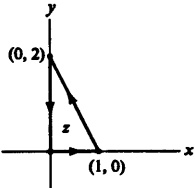
\includegraphics[width=0.20\textwidth]{figures/ch4_img_in_image_box_404_245_599_433.jpg}
\end{center}

\item Let  $ \alpha = (2x + y \cos xy)dx + (x \cos xy)dy $ on  $ \mathbb{R}^2 $. Show that  $ \alpha $ is closed. Show that  $ \alpha $ is exact by finding a function  $ f $:  $ \mathbb{R}^2 \to \mathbb{R} $ with  $ \alpha = df $. What would the integral of  $ \alpha $ over the cycle of Exercise 13 be?

\item Let

\[
\alpha=\frac{1}{2\pi}\frac{x\,dy-y\,dx}{x^{2}+y^{2}}.
\]

Prove that $\alpha$ is a closed 1-form on $\mathbb{R}^2 - \{0\}$. Compute the integral of $\alpha$ over the unit circle $S^1$. How does this result show that $\alpha$ is not exact? How does this show that $\delta i(\alpha)$ is not exact, where $i: S^1 \to \mathbb{R}^2$ is the canonical imbedding?

\item (a) Prove that every closed 1-form on  $ S^{2} $ is exact.

(b) Let

\[
\sigma=\frac{r_{1}\,d r_{2}\wedge d r_{3}-r_{2}\,d r_{1}\wedge d r_{3}+r_{3}\,d r_{1}\wedge d r_{2}}{(r_{1}^{2}+r_{2}^{2}+r_{3}^{2})^{3/2}}
\]

in  $ \mathbb{R}^{3} - \{0\} $. Prove that  $ \sigma $ is closed.

(c) Evaluate  $ \int_{S^{2}}\sigma $. How does this show that  $ \sigma $ is not exact?

(d) Let

\[
\alpha=\frac{r_{1}d r_{1}+r_{2}d r_{2}+\cdots+r_{n}d r_{n}}{(r_{1}^{2}+r_{2}^{2}+\cdots+r_{n}^{2})^{n/2}}
\]

in  $ \mathbb{R}^n - \{0\} $. Find  $ *\alpha $, and prove that  $ *\alpha $ is closed.

(e) Evaluate  $ \int_{S^{n-1}} \ast \alpha $. Is  $ \ast \alpha $ exact?

\item Using de Rham cohomology, prove that the torus $T^{2}$ is not diffeomorphic with the 2-sphere $S^{2}$.

\item (a) Prove that every closed 1-form in the open shell

\[
1<\left(\sum_{i=1}^{3}r_{i}^{2}\right)^{1/2}<2
\]

in $\mathbb{R}^{3}$ is exact.

(b) Find a 2-form in the above shell that is closed but not exact.

(c) Prove that the above shell is not diffeomorphic with the open unit ball in  $ \mathbb{R}^{3} $.

\item Let $f$ and $g$ be $C^\infty$ maps of $M$ into $N$ which are $C^\infty$ homotopic; that is, there exists a $C^\infty$ map $F$ of $M \times(-\varepsilon,1+\varepsilon)$ into $N$, for some $\varepsilon>0$, such that $F(m,0)=f(m)$ and $F(m,1)=g(m)$ for every $m\in M$. Prove that the induced homomorphisms $f^*$ and $g^*$ of $H_{\mathrm{de\,R}}^{p}(N)$ into $H_{\mathrm{de\,R}}^{p}(M)$ are equal for each integer $p$. (Hint: You will need to prove that the two injections $i_{0}(m)=(m,0)$ and $i_{1}(m)=(m,1)$ of $M$ into $M\times(-\varepsilon,1+\varepsilon)$ induce the same homomorphisms on de Rham cohomology. To prove this, find suitable homotopy operators. The outline of the proof of the Poincaré \hyperref[thm:4.18]{lemma 4.18} should be helpful.)

\item (a) Let $f: M^n \to \mathbb{R}^{n+1}$ be an immersion, and let $M^n$ be given the induced Riemannian structure; that is, for $m \in M$ and $u, v \in M_m$,

\[
\langle u,v\rangle_{m}=\langle d f(u),d f(v)\rangle_{f(m)}.
\]

Suppose that $M$ is oriented, and that $\vec{n}$ is the oriented unit normal field along $f(M^n)$. (This means that $\vec{n}, df(v_1), \ldots, df(v_n)$ is to be an oriented orthonormal basis of the tangent space to Euclidean space at $f(m)$ whenever $v_1, \ldots, v_n$ is an oriented orthonormal basis of $M_m$.) Show that the volume form on $M$ is given by

\[
\omega=\delta f\big(i(\vec{n})(dr_{1}\wedge\cdots\wedge dr_{n+1})\big).
\]

(b) Let $D$ be an open set in the xy plane, and let $\varphi: D \to \mathbb{R}^3$ be a smooth map of the form

\[
\varphi(x,y)=\bigl(x,y,f(x,y)\bigr).
\]

Thus $\varphi$ determines an imbedded surface in $\mathbb{R}^{3}$. Give $D$ and $\mathbb{R}^{3}$ the standard orientations. Use part (a) to prove that the induced volume form on $D$ is given by

\[
\omega=\left(\sqrt{\left(\frac{\partial f}{\partial x}\right)^{2}+\left(\frac{\partial f}{\partial y}\right)^{2}+1}\right)\,dx\wedge dy.
\]

\end{problemset}

% Chapter 5 — Sheaves, Cohomology, and the de Rham Theorem (reviewed)
\chapter{Sheaves, Cohomology, and the de Rham Theorem}

SHEAVES,

COHOMOLOGY,

and the DE RHAM THEOREM

The principal objective in this chapter is a proof of the de Rham theorem, one version of which we have stated in 4.17. In its most complete form it asserts that the homomorphism from the de Rham cohomology ring to the differentiable singular cohomology ring given by integration of closed forms over differentiable singular cycles is a ring isomorphism. The approach will be to exhibit both the de Rham cohomology and the differentiable singular cohomology as special cases of sheaf cohomology and to use a basic uniqueness theorem for homomorphisms of sheaf cohomology theories to prove that the natural homomorphism between the de Rham and differentiable singular theories is an isomorphism. As an added dividend of this approach we shall also obtain the existence of canonical isomorphisms of the de Rham and differentiable singular cohomology theories with the continuous singular theory, the Alexander-Spanier theory, and the Czech cohomology theory for differentiable manifolds. From these isomorphisms we shall conclude that the de Rham cohomology theory is a topological invariant of a differentiable manifold.

No previous knowledge of sheaf theory nor of any of these cohomology theories is assumed. We shall develop those aspects of the theories necessary for our applications. We begin with an introduction to the theory of sheaves and sheaf cohomology. Our approach is based largely on the development given by Cartan in [4]. The interested reader will find more general treatments of sheaf theory in Cartan [4], Godement [7], and Bredon [3]. Sheaves are a very powerful tool in the study of complex manifolds. For an excellent account of their use in the theory of Riemann surfaces, see Gunning [8].

Let M be a differentiable manifold. Recall that M is assumed to be second countable and is therefore paracompact. It should be pointed out that nearly all of the sheaf theory presented in this chapter depends only on M being a paracompact Hausdorff space. The differentiable structure on M will be invoked only in a few examples and in the discussions of the Rham cohomology (5.28) and the differentiable singular cohomology (5.31); and, in addition, the locally Euclidean structure will be invoked in the discussion of the singular cohomology (5.31). Otherwise, M need only be a paracompact Hausdorff space.

Throughout this chapter, K will be a fixed principal ideal domain. We shall treat sheaves of K-modules over M. The most important cases to keep in mind are these: \index{K-modules}

(i) K is the ring of integers Z, whence a K-module is simply an abelian group.

(ii) K is the field of real numbers  $ \mathbb{R} $, whence a K-module is simply a real vector space.

For the first few sections of this chapter, K could be any ring. The additional property that K is a principal ideal domain will be used first in 5.13.

\section{Sheaves and Presheaves}


\begin{definition}\label{thm:5.1}
A sheaf $\mathcal{S}$ of $K$-modules over $M$ consists of a topological space $\mathcal{S}$ together with a map $\pi\colon \mathcal{S} \to M$ satisfying:

(a)  $ \pi $ is a local homeomorphism of S onto  $ M $.

(b)  $ \pi^{-1}(m) $ is a K-module for each  $ m \in M $.

(c) The composition laws are continuous in the topology on S.

We elaborate on (c). Let $\mathcal{S}\circ\mathcal{S}$ be the subspace of $\mathcal{S}\times\mathcal{S}$ consisting of all pairs $(s_1,s_2)$ such that $\pi(s_1)=\pi(s_2)$. Then (c) requires that the map $(s_1,s_2)\mapsto s_1-s_2$ of $\mathcal{S}\circ\mathcal{S}\to\mathcal{S}$ be continuous, and that each of the maps $s\mapsto k s$ of $\mathcal{S}\to\mathcal{S}$ for $k\in K$ be continuous. It follows easily that the maps $s\mapsto(-s)$ and $(s_1,s_2)\mapsto s_1+s_2$ also are continuous. Sheaves of $K$ algebras are defined similarly, with the additional requirement in (c) that the map $(s_1,s_2)\mapsto s_1\cdot s_2$ of $\mathcal{S}\circ\mathcal{S}\to\mathcal{S}$ be continuous.

The map $\pi$ is called the projection; and the $K$-module $\mathcal{S}_m = \pi^{-1}(m)$ is called the stalk over $m \in M$. Let $U \subset M$ be open. A continuous map $f: U \to \mathcal{S}$ such that $\pi \circ f = id$ is called a section of $\mathcal{S}$ over $U$. The 0-section is the section which associates with $m \in U$ the zero element of $\mathcal{S}_m$. We let $\Gamma(\mathcal{S}, U)$ denote the set of sections of $\mathcal{S}$ over $U$. We make $\Gamma(\mathcal{S}, U)$ into a $K$-module as follows. Let $f$ and $g$ belong to $\Gamma(\mathcal{S}, U)$, and let $k \in K$. We define the sum of $f$ and $g$ to be the section

\[
(f+g)(m)=f(m)+g(m)\qquad(m\in U),
\]

and we define a section $kf$ by setting

\[
(k f)(m)=k\bigl(f(m)\bigr)\qquad(m\in U).
\]

With these operations, $\Gamma(\mathcal{S},U)$ becomes a $K$-module. The module of sections of $\mathcal{S}$ over $M$ (global sections) will simply be denoted by $\Gamma(\mathcal{S})$. Observe that since $\pi$ is a local homeomorphism, sections are open maps; and if sections $f$ and $g$ agree at $m\in M$, then they must agree on a neighborhood of $m$.

\end{definition}

\begin{examples}\label{thm:5.2}
The most elementary example of a sheaf over $M$ is that of a so-called constant sheaf $\mathcal{G} = M \times G$, where $G$ is a $K$-module with the discrete topology and $\mathcal{G}$ is given the product topology. Here the projection is simply $\pi(m,g) = m$. \index{Constant sheaf}

A less trivial example is the following. Let $\bar{F}_{m}$ denote the set of germs of $C^{\infty}$ functions at $m\in M$ (as in 1.13), and let

\begin{equation}
\label{eq:5.2:1}
\mathcal{C}^{\infty}(M)=\bigcup_{m\in M}\bar{F}_{m}.
\end{equation}

When it will introduce no confusion, we shall denote $\mathcal{C}^{\infty}(M)$ simply by $\mathcal{C}^{\infty}$. We define the projection $\pi\colon \mathcal{C}^{\infty} \to M$ in the obvious fashion so that $f \in \bar{F}_{\pi(f)}$. Associate with each open set $U$ in $M$ and each $C^{\infty}$ function $f$ on $U$ the set

\[
\bigcup_{m\in U}f_{m}\subset\mathcal{C}^{\infty},
\]

where  $ f_m $ is the germ of  $ f $ at  $ m $. The collection of these sets forms a basis for a topology on  $ \mathcal{C}^\infty $ which makes  $ \mathcal{C}^\infty $ into a sheaf of real vector spaces (in fact, a sheaf of algebras since each  $ \bar{F}_m $ has an algebra structure).  $ \mathcal{C}^\infty(M) $ is called the sheaf of germs of  $ C^\infty $ functions on  $ M $. Similarly, one constructs the sheaf  $ \mathcal{C}^p(M) $ of germs of functions of class  $ C^p $ on  $ M $ for each integer  $ p \geq 0 $. \index{Sheaf}

\end{examples}

\begin{remarks}\label{thm:5.3}
One should be cautioned that sheaves are generally not Hausdorff spaces. A simple example is provided by the sheaf  $ \mathcal{C}^0(\mathbb{R}) $ of germs of continuous functions on the real line. Let  $ g(t) \equiv 0 $, let  $ f(t) = 0 $ for  $ t \leq 0 $, and let  $ f(t) = t $ for  $ t > 0 $. Then the germs of  $ f $ and  $ g $ at the origin are distinct elements of  $ \mathcal{C}^0(\mathbb{R}) $; however,  $ f $ and  $ g $ have the same germ for each  $ t < 0 $. It follows that the germs of  $ f $ and  $ g $ at the origin cannot be separated by disjoint open sets in  $ \mathcal{C}^0(\mathbb{R}) $.

\end{remarks}

\begin{definition}\label{thm:5.4}
Let $\mathcal{S}$ and $\mathcal{S}'$ be sheaves on $M$ with projections $\pi$ and $\pi'$ respectively. A continuous map $\varphi\colon \mathcal{S} \to \mathcal{S}'$ such that  $ \pi' \circ \varphi = \pi $ is called a sheaf mapping. Observe that sheaf mappings are necessarily local homeomorphisms, and they map stalks into stalks. A sheaf mapping  $ \varphi $ which is a homomorphism (of K-modules) on each stalk is called a sheaf homomorphism. A sheaf isomorphism is a sheaf homomorphism with an inverse which is also a sheaf homomorphism.

An open set $\mathcal{R}$ in the sheaf $\mathcal{S}$ such that the subset $\mathcal{R}_m = \mathcal{R} \cap \mathcal{S}_m$ is a submodule of $\mathcal{S}_m$ for each $m \in M$ is called a subsheaf of $\mathcal{S}$. It is clear that a subsheaf of $\mathcal{S}$, with the natural topology and the projection map which it inherits from $\mathcal{S}$, is again a sheaf.

Let $\varphi: \mathcal{S} \to \mathcal{T}$ be a homomorphism of sheaves. The kernel of $\varphi$ (ker $\varphi$) is the subset of $\mathcal{S}$ which maps under $\varphi$ into the 0-section of $\mathcal{T}$, and is in fact a subsheaf of $\mathcal{S}$. The subsheaf $\varphi(\mathcal{S}) \subset \mathcal{T}$ is called the image of $\varphi$ (im $\varphi$). In the case in which $\varphi$ is one-to-one, we shall often identify $\mathcal{S}$ with $\varphi(\mathcal{S})$ and speak of the subsheaf $\mathcal{S}$ of $\mathcal{T}$.

Let $\mathcal{R}$ be a subsheaf of $\mathcal{S}$. For each $m\in M$, let $\mathcal{T}_{m}$ denote the quotient module $\mathcal{S}_{m}/\mathcal{R}_{m}$, and let

\begin{equation}
\label{eq:5.4:1}
\mathcal{T}=\bigcup_{m\in M}\mathcal{T}_{m}.
\end{equation}

Let $\tau: \mathcal{S} \to \mathcal{T}$ be the natural map which associates with each element of $\mathcal{S}_m$ its coset in $\mathcal{T}_m$, for each $m$, and give $\mathcal{T}$ the quotient topology. That is, a set $U$ in $\mathcal{T}$ will be open if and only if $\tau^{-1}(U)$ is open in $\mathcal{S}$. Then, with this topology and with the natural projection which maps each element of $\mathcal{T}_m$ to $m$, $\mathcal{T}$ is a sheaf over $M$ and $\tau: \mathcal{S} \to \mathcal{T}$ is a sheaf homomorphism. We leave the details as an exercise. $\mathcal{T}$ is called the quotient sheaf of $\mathcal{S}$ modulo $\mathcal{R}$. \index{Quotient sheaf}

If $\varphi: \mathcal{S} \to \mathcal{T}$ is a homomorphism of sheaves, then it is easily checked that the natural map $\mathcal{S}/\ker \varphi \to \mathrm{im} \varphi$ given by $(s + (\ker \varphi \mid \mathcal{S}_m)) \mapsto \varphi(s)$ for $s \in \mathcal{S}_m$ is a sheaf isomorphism.

A sequence of sheaves and homomorphisms

\begin{equation}
\label{eq:5.4:2}
\cdots\to\mathcal{S}_{i}\to\mathcal{S}_{i+1}\to\mathcal{S}_{i+2}\to\cdots
\end{equation}

is called exact if at each stage the image of a given homomorphism is the kernel of the next. Exact sequences of K-modules are defined similarly. Observe that (2) is exact if and only if for each $m\in M$ the induced sequence of homomorphisms of the stalks over $m$, namely,

\begin{equation}
\label{eq:5.4:3}
\cdots\to(\mathcal{S}_{i})_{m}\to(\mathcal{S}_{i+1})_{m}\to(\mathcal{S}_{i+2})_{m}\to\cdots,
\end{equation}

is exact. If $\mathcal{R}$ is a subsheaf of $\mathcal{S}$, and $\mathcal{T}$ is the quotient sheaf $\mathcal{S}/\mathcal{R}$, then the natural sequence of homomorphisms

\begin{equation}
\label{eq:5.4:4}
0\to\mathcal{R}\to\mathcal{S}\to\mathcal{T}\to0
\end{equation}

is exact, where 0 denotes the constant sheaf over M whose stalk over each point is the trivial K-module consisting of only one element. Exact sequences of the form (4) consisting of only five terms with the first and last being the 0 sheaf are called short exact sequences. Short exact sequences of K-modules are defined similarly.

\end{definition}

\subsection{Presheaves}\label{thm:5.5} A presheaf $P = \{S_U; \rho_{U,V}\}$ of $K$-modules on $M$ consists of a $K$-module $S_U$ for each open set $U$ in $M$ and a homomorphism $\rho_{U,V}: S_V \to S_U$ for each inclusion $U \subset V$ of open sets in $M$, such that $\rho_{U,U} = \mathrm{id}$, and such that whenever $U \subset V \subset W$, the following diagram commutes: \index{Presheaf}

\begin{equation}
\label{eq:5.5:1}
\begin{tikzpicture}[baseline={(current bounding box.center)},>=stealth]
\node (SW) at (0,1.4) {$S_W$};
\node (SV) at (2.2,1.4) {$S_V$};
\node (SU) at (1.1,0) {$S_U$};
\draw[->] (SW) -- node[above] {$\rho_{V,W}$} (SV);
\draw[->] (SW) -- node[left] {$\rho_{U,W}$} (SU);
\draw[->] (SV) -- node[right] {$\rho_{U,V}$} (SU);
\end{tikzpicture}
\end{equation}

A typical example of a presheaf is the following. Associate with each open set $U$ in $M$ the algebra $C^\infty(U)$ of $C^\infty$ functions on $U$, and let $\rho_{U,V}$ be the map which restricts a $C^\infty$ function on $V$ to a $C^\infty$ function on $U$. This yields a presheaf $\{C^\infty(U);\rho_{U,V}\}$ of real vector spaces (in fact algebras) on $M$. Similarly, one could associate with $U$ the vector space of $p$-forms on $U$ for some fixed $p$ and again let $\rho_{U,V}$ be the restriction mapping.

Let $P=\{S_{U};\rho_{U,V}\}$ and $P^{\prime}=\{S_{U}^{\prime};\rho_{U,V}^{\prime}\}$ be presheaves on $M$. By a presheaf homomorphism of $P$ to $P^{\prime}$ we mean a collection $\{\varphi_{U}\}$ of homomorphisms $\varphi_{U}\colon S_{U}\to S_{U}^{\prime}$ such that

\begin{equation}
\label{eq:5.5:2}
\rho_{U,V}^{\prime}\circ\varphi_{V}=\varphi_{U}\circ\rho_{U,V}
\end{equation}

whenever $U \subset V$. A presheaf isomorphism is a presheaf homomorphism $\{\varphi_{U}\}$ in which each $\varphi_{U}$ is an isomorphism of $K$-modules.

\subsection{The Relationship between Sheaves and Presheaves}\label{thm:5.6} Each sheaf  $ \mathcal{S} $ gives rise canonically to a presheaf  $ \{\Gamma(\mathcal{S},U);\rho_{U,V}\} $. Here we associate with each open set  $ U $ in  $ M $ the  $ K $-module  $ \Gamma(\mathcal{S},U) $ of sections of  $ \mathcal{S} $ over  $ U $, and to each inclusion  $ U \subset V $ of open sets in  $ M $ we associate the homomorphism

\begin{equation}
\label{eq:5.6:1}
\rho_{U,V}\colon\Gamma(\mathcal{S},V)\to\Gamma(\mathcal{S},U)
\end{equation}

which maps a section of $\mathcal{S}$ over $V$ to its restriction to U. We shall denote this map of sheaves to presheaves by $\alpha$. We call $\alpha(\mathcal{S})$ the presheaf of sections of the sheaf $\mathcal{S}$.

Conversely, we shall now show that each presheaf canonically determines a sheaf, which we call its associated sheaf. In practice, many sheaves will in this manner arise naturally from presheaves. The best example to keep in mind during the following construction is the presheaf  $ \{C^\infty(U);\rho_{U,V}\} $; its associated sheaf will be the sheaf of germs of  $ C^\infty $ functions on  $ M $.

Let $P = \{S_U; \rho_{U,V}\}$ be a presheaf of $K$-modules on $M$. Let $m \in M$, and let $S_m^*$ be the disjoint union of each of the modules $S_U$ for which $m \in U$. If we set $f \in S_U$ equivalent to $g \in S_V$ if and only if there is a neighborhood $W$ of $m$ with $W \subset U \cap V$ such that $\rho_{W,U}f = \rho_{W,V}g$, we obtain an equivalence relation on $S_m^*$. The set $S_m$ of equivalence classes of elements of $S_m^*$ will be the stalk of the associated sheaf over $m$. If $m \in U$, let $\rho_{m,U}: S_U \to S_m$ be the natural projection which assigns to each element of $S_U$ its equivalence class. Let $f \in S_U$ and $g \in S_V$ be representatives of classes $s_1$ and $s_2$ in $S_m$ respectively. There exists a neighborhood $W$ of $m$ such that $W \subset U \cap V$. Define addition in $S_m$ by setting

\begin{equation}
\label{eq:5.6:3}
s_{1}+s_{2}=\rho_{m,w}(\rho_{W,U}f+\rho_{W,V}g),
\end{equation}

and define multiplication by  $ k \in K $ by setting

\begin{equation}
\label{eq:5.6:4}
k s_{1}=\rho_{m,U}(k f).
\end{equation}

It is easy to check that the operations in (3) and (4) are well-defined and give $S_{m}$ the structure of a $K$-module such that the maps $\rho_{m,U}$ are all homomorphisms. $S_{m}$ is known as the direct limit of the modules $S_{U}$ for $U$ containing $m$. Now let \index{Direct limit of K-modules}

\begin{equation}
\label{eq:5.6:5}
\mathcal{S}=\bigcup_{m\in M}\mathcal{S}_{m},
\end{equation}

and let $\pi: \mathcal{S} \to M$ be the obvious projection such that $\pi(\mathcal{S}_m) = m$. We topologize $\mathcal{S}$ by taking for a basis of the topology the collection of subsets of $\mathcal{S}$ of the form

\begin{equation}
\label{eq:5.6:6}
O_{f}=\{\rho_{p,U}f\colon p\in U\}
\end{equation}

for the various $f\in S_U$ and the various open sets $U$ in $M$. This collection does indeed form a basis for a topology on $\mathcal{S}$, for if $s\in O_f\cap O_g$, say $s=\rho_{p,U}f=\rho_{p,V}g$, then there is a neighborhood $W$ of $p$ with $W\subset U\cap V$ for which $\rho_{W,U}f=\rho_{W,V}g$, from which it follows that $s\in O_{\rho_{W,U}f}\subset O_f\cap O_g$.

We claim that $\mathcal{S}$ is a sheaf over $M$ with projection $\pi$. Now $\pi$ is a local homeomorphism since it is a homeomorphism on each $O_f$. Each stalk $\mathcal{S}_m$ has been given the structure of a $K$-module, so finally we need only check that the composition operations are continuous. Consider first multiplication by $k \in K$. Let $s \in \mathcal{S}$, and let $O$ be an open neighborhood of $ks$. Let $s = \rho_{p,U}f$. Then $O_{k f}$ is also an open neighborhood of $ks$. Let $V$ be a neighborhood of $p$ contained in $\pi(O_{k f} \cap O)$. Then $O_{\rho_{V,U}f}$ is an open neighborhood of $s$ which maps under multiplication by $k$ into the open neighborhood $O_{\rho_{V,U}kf} \subset O$ of $ks$. Finally, we show that the map $(s_1, s_2) \mapsto s_1 - s_2$ of $\mathcal{S} \circ \mathcal{S} \to \mathcal{S}$ is continuous. For let $O_f$ be an open neighborhood of $s_1 - s_2$, say $s_1 - s_2 = \rho_{p,U}f$, and let $s_1 = \rho_{p,V}g$ and $s_2 = \rho_{p,W}h$. Then there exists an open neighborhood $Q$ of $p$ with $Q \subset U \cap V \cap W$ such that

\begin{equation}
\label{eq:5.6:7}
\rho_{Q,U}f=\rho_{Q,V}g-\rho_{Q,W}h.
\end{equation}

It follows that the open neighborhood

\begin{equation}
\label{eq:5.6:8}
O_{\rho_{Q,V}g}\times O_{\rho_{Q,W}h}\cap\mathcal{S}\circ\mathcal{S}
\end{equation}

of $(s_{1}, s_{2})$ maps into $O_{f}$. Thus the composition operations are continuous, and $\mathcal{S}$ is a sheaf over $M$ with projection $\pi$. $\mathcal{S}$ is called the sheaf associated with the presheaf $P$. We shall denote this map of presheaves to sheaves by $\beta$; thus $\mathcal{S} = \beta(P)$.

Clearly, each sheaf homomorphism $\varphi\colon\mathcal{S}\to\mathcal{T}$ gives rise to a presheaf homomorphism between the presheaves of sections $\alpha(\mathcal{S})$ and $\alpha(\mathcal{T})$ by composing elements of $\Gamma(\mathcal{S},U)$ with $\varphi$. Conversely, a presheaf homomorphism $\{\varphi_U\}$ from $P$ to $P'$ canonically induces a homomorphism $\varphi$ of the associated sheaves $\beta(P)$ and $\beta(P')$ such that

\begin{equation}
\label{eq:5.6:9}
\rho_{p,U}^{\prime}\circ\varphi_{U}=\varphi\circ\rho_{p,U}
\end{equation}

for each open set $U$ in $M$ and each $p \in U$. Moreover, in going in either direction, from homomorphisms of sheaves to homomorphisms of presheaves, or vice versa, the composition of two homomorphisms induces the composition of the corresponding homomorphisms.

Suppose now that we start with a sheaf $\mathcal{S}$, take its presheaf $\alpha(\mathcal{S})$ of sections, and then form the associated sheaf $\beta(\alpha(\mathcal{S}))$, thus obtaining the sheaf of germs of sections of $\mathcal{S}$. Then the sheaves $\mathcal{S}$ and $\beta(\alpha(\mathcal{S}))$ are canonically isomorphic. Indeed, let $\xi \in \beta(\alpha(\mathcal{S}))$ be the germ at $p$ of some section $f$ of $\mathcal{S}$ over an open set $U$ containing $p$; that is, $\xi = \rho_{p,U}f$ for $f \in \Gamma(\mathcal{S}, U)$. Then $\xi \mapsto f(p)$ determines a well-defined map $\beta(\alpha(\mathcal{S})) \to \mathcal{S}$ which is a sheaf isomorphism. We leave the details as an exercise.

Generally, however, if we start with a presheaf $P$ and take the presheaf $\alpha(\beta(P))$ of sections of the sheaf associated with $P$, we may get a presheaf quite distinct from $P$. For example, let $P = \{S_U; \rho_{U,V}\}$ where $S_U$ is the principal ideal domain $K$ for each $U$, and all restrictions $\rho_{U,V}$ for $U \subsetneq V$ are identically 0. Then the presheaf $\alpha(\beta(P))$ assigns to each open set $U$ in $M$ the zero $K$-module. The conditions of the following definition are clearly necessary if $P$ is to be isomorphic with $\alpha(\beta(P))$, and it will be shown in §5.8 that they are also sufficient.

\begin{definition}\label{thm:5.7}
A presheaf $\{S_{U};\rho_{U,V}\}$ on $M$ is said to be complete if whenever the open set $U$ is expressed as a union $\bigcup U_{\alpha}$ of open sets in $M$, the following two conditions are satisfied:

$(C_{1})'$ Whenever $f$ and $g$ in $S_{U}$ are such that $\rho_{U_{\alpha},U}f = \rho_{U_{\alpha},U}g$ for all $\alpha$, then $f = g$.

$(C_{2})$ Whenever there is an element $f_{\alpha}\in S_{U_{\alpha}}$ for each $\alpha$ such that $\rho_{U_{\alpha}\cap U_{\beta},U_{\alpha}}f_{\alpha}=\rho_{U_{\alpha}\cap U_{\beta},U_{\beta}}f_{\beta}$ for all $\alpha$ and $\beta$, then there exists $f\in S_{U}$ such that $f_{\alpha}=\rho_{U_{\alpha},U}f$ for each $\alpha$.

\end{definition}

\begin{proposition}\label{thm:5.8}
If $P$ is a complete presheaf, then $\alpha(\beta(P))$ is canonically isomorphic with $P$.

\end{proposition}

\begin{proof}
Let $P=\{S_{U};\rho_{U,V}\}$. We define a presheaf homomorphism from $P$ to $\alpha(\beta(P))$ as follows. For each open set $U$ in $M$ we map

\begin{equation}
\label{eq:5.8:1}
S_{U}\to\Gamma\bigl(\beta(P),U\bigr)
\end{equation}

by sending the element f of  $ S_{U} $ to the section

\begin{equation}
\label{eq:5.8:2}
p\mapsto\rho_{p,U}f
\end{equation}

of $\beta(P)$ over $U$. To prove that this presheaf homomorphism is an isomorphism, we need to prove that each of the homomorphisms (1) are isomorphisms. Injectivity follows from $5.7(C_{1})$, for if $f$ in $S_{U}$ maps to the 0-section, then there exists a cover $\{U_{\alpha}\}$ of $U$ such that $\rho_{U_{\alpha},U}f=\rho_{U_{\alpha},U}(0)$. Therefore $f=0\in S_{U}$ by $(C_{1})$. To prove surjectivity, let $c$

be a section of $\beta(P)$ over $U$. Then for each $p \in U$, there is a neighborhood $U_p$ of $p$ and an element $f_p \in S_{U_p}$ such that

\begin{equation}
\label{eq:5.8:3}
\rho_{q,U_{p}}f_{p}=c(q)
\end{equation}

for all $q\in U_{p}$. It follows from (3) and $5.7(C_{1})$ that for each $p$ and $q$ in $U$,

\begin{equation}
\label{eq:5.8:4}
\rho_{U_{p}\cap U_{q},U_{p}}f_{p}=\rho_{U_{p}\cap U_{q},U_{q}}f_{q}.
\end{equation}

Thus, according to 5.7($C_{2}$), there exists $f \in S_{U}$ such that

\begin{equation}
\label{eq:5.8:5}
f_{p}=\rho_{U_{p},U}f
\end{equation}

for each $p \in U$. It follows from (5), (3), and (2) that $f$ maps to $c$ under the homomorphism (1).

\end{proof}

\subsection{Tensor Products}\label{thm:5.9} Before we define the tensor products of sheaves and presheaves, we need a few preliminary remarks. The definition of the tensor product  $ S \otimes T $ of K-modules S and T is completely analogous to that for the special case 2.1 of tensor products of $R$-modules. If  $ f: S \to S' $ and  $ h: T \to T' $ are homomorphisms of K-modules, then their tensor product  $ f \otimes h $ is the homomorphism of  $ S \otimes T $ into  $ S' \otimes T' $ uniquely associated by the universal mapping property \hyperref[thm:2.2]{2.2(a)} with the bilinear map

\begin{equation}
\label{eq:5.9:1}
(s,t)\mapsto f(s)\otimes h(t)
\end{equation}

of  $ S \times T $ into  $ S' \otimes T' $.

Observe that if S is a K-module, then there is a canonical isomorphism

\begin{equation}
\label{eq:5.9:2}
S\otimes K\cong S.
\end{equation}

Indeed, let $f: S \otimes K \to S$ be the homomorphism determined by the bilinear map $(s, k) \mapsto ks$ of $S \times K \to S$. Then $f$ is clearly surjective, and is also injective since $\sum_{i}(s_{i} \otimes k_{i}) = \left(\sum_{i} k_{i} s_{i}\right) \otimes 1$, so if $f\left(\sum_{i}(s_{i} \otimes k_{i})\right) = 0$, then $\sum_{i} k_{i} s_{i} = 0$, which implies $\sum_{i}(s_{i} \otimes k_{i}) = 0$.

Now let $P=\{S_{U};\rho_{U,V}\}$ and $P^{\prime}=\{S_{U}^{\prime};\rho_{U,V}^{\prime}\}$ be presheaves on $M$. Then their tensor product is the presheaf

\begin{equation}
\label{eq:5.9:3}
\begin{array}{r}{P\otimes P^{\prime}=\{S_{U}\otimes S_{U}^{\prime};\rho_{U,V}\otimes\rho_{U,V}^{\prime}\}.}\end{array}
\end{equation}

If $\{\varphi_U\}$: $P \to Q$ and $\{\varphi'_U\}$: $P' \to Q'$ are homomorphisms of presheaves (\eqref{eq:5.5:2}), then their tensor product $\{\varphi_U\} \otimes \{\varphi'_U\}$ is by definition the homomorphism $\{\varphi_U \otimes \varphi'_U\}$ of $P \otimes P'$ into $Q \otimes Q'$.

If $\mathcal{S}$ and $\mathcal{T}$ are sheaves over $M$, we define their tensor product $\mathcal{S} \otimes \mathcal{T}$ to be the sheaf associated with the tensor product of the presheaves of sections of $\mathcal{S}$ and $\mathcal{T}$. That is,

\begin{equation}
\label{eq:5.9:4}
\mathcal{S}\otimes\mathcal{T}=\beta\big(\alpha(\mathcal{S})\otimes\alpha(\mathcal{T})\big).
\end{equation}

Moreover, if $\varphi: \mathcal{S} \to \mathcal{T}$ and $\gamma: \mathcal{S}' \to \mathcal{T}'$ are sheaf homomorphisms, and if $\{\varphi_U\}: \alpha(\mathcal{S}) \to \alpha(\mathcal{T})$ and $\{\gamma_U\}: \alpha(\mathcal{S}') \to \alpha(\mathcal{T}')$ are the corresponding homomorphisms on the presheaves of sections, then we define the tensor product $\varphi \otimes \gamma$ to be the homomorphism $\mathcal{S} \otimes \mathcal{S}' \to \mathcal{T} \otimes \mathcal{T}'$ associated with the presheaf homomorphism

\begin{equation}
\label{eq:5.9:5}
\{\varphi_{U}\}\otimes\{\gamma_{U}\}\colon\alpha(\mathcal{S})\otimes\alpha(\mathcal{S}^{\prime})\to\alpha(\mathcal{T})\otimes\alpha(\mathcal{T}^{\prime}).
\end{equation}

The reader should check that there is a canonical isomorphism

\begin{equation}
\label{eq:5.9:6}
(\mathcal{S}\otimes\mathcal{T})_{m}\cong\mathcal{S}_{m}\otimes\mathcal{T}_{m},
\end{equation}

so in particular if $\mathcal{K}$ is the constant sheaf $M\times K$, then in view of (2) there is a canonical isomorphism

\begin{equation}
\label{eq:5.9:7}
\mathcal{S}\otimes\mathcal{K}\cong\mathcal{S}.
\end{equation}

Moreover, if $\varphi$ and $\gamma$ are sheaf homomorphisms as above, then the reader should check that

\begin{equation}
\label{eq:5.9:8}
(\varphi\otimes\gamma)\bigm|(\mathcal{S}\otimes\mathcal{S}^{\prime})_{m}=\varphi\bigm|\mathcal{S}_{m}\otimes\gamma\bigm|\mathcal{S}_{m}^{\prime}.
\end{equation}

One might ask, “Why not define $\mathcal{S}\otimes\mathcal{T}$ and $\varphi\otimes\gamma$ by (6) and (8) rather than going to presheaves and back?” We could indeed proceed in this way, but it would involve a considerable duplication of previous work. The reason is that if we define the tensor products by (6) and (8), then we would also have to define the topology on $\mathcal{S}\otimes\mathcal{T}$ and check that the properties $5.1(a)$ and (c) are satisfied, and would also have to prove that $\varphi\otimes\gamma$ is continuous. In defining $\mathcal{S}\otimes\mathcal{T}$ and $\varphi\otimes\gamma$ by going to presheaves and back, the work of showing that $\mathcal{S}\otimes\mathcal{T}$ is really a sheaf and that $\varphi\otimes\gamma$ is a sheaf homomorphism has already been carried out in the analysis of the maps $\alpha$ and $\beta$ of 5.6.

\subsection{Fine Sheaves}\label{thm:5.10} A sheaf $\mathcal{S}$ over $M$ is said to be fine if for each locally finite cover  $ \{U_{i}\} $ of M by open sets there exists for each i an endomorphism  $ l_{i} $ of S such that:

(a) $\operatorname{supp}(l_i) \subset U_i$.

(b)  $ \sum_{i} l_{i} = id $.

Here, by $\operatorname{supp}(l_{i})$ (the support of $l_{i}$) we mean the closure of the set of points in $M$ for which $l_{i} \bigm| \mathcal{S}_{m}$ is not zero. We shall call $\{l_{i}\}$ a partition of unity for $\mathcal{S}$ subordinate to the cover $\{U_{i}\}$ of $M$.

An example of a fine sheaf is the sheaf  $ \mathcal{C}^{\infty}(M) $ of germs of  $ C^{\infty} $ functions on  $ M $. If  $ \{U_i\} $ is a locally finite open cover of  $ M $, let  $ \{\varphi_i\} $ be a partition of unity on  $ M $ subordinate to this cover (\hyperref[thm:1.11]{Theorem 1.11}). We obtain endomorphisms  $ \tilde{l}_i $ of the presheaf  $ \{C^{\infty}(U);\rho_{U,V}\} $ by setting

\begin{equation}
\label{eq:5.10:1}
\tilde{l}_{i}(f)=(\varphi_{i}\bigm|U)\cdot f\quad\mathsf{f o r}f\in C^{\infty}(U).
\end{equation}

The associated sheaf endomorphisms $l_{i}$ of $\mathcal{C}^{\infty}(M)$ form a partition of unity subordinate to the cover $\{U_{i}\}$ of $M$.

Let $\mathcal{S}$ and $\mathcal{T}$ be sheaves over $M$, with $\mathcal{S}$ fine. Then $\mathcal{S} \otimes \mathcal{T}$ is itself a fine sheaf. Indeed, if $\{l_i\}$ is a partition of unity for $\mathcal{S}$ subordinate to the cover $\{U_i\}$ of $M$, then $\{l_i \otimes \mathrm{id}\}$ is a partition of unity for $\mathcal{S} \otimes \mathcal{T}$.

\subsection{\quad}\label{thm:5.11} A sheaf homomorphism $\varphi: \mathcal{S} \to \mathcal{T}$ gives rise to a homomorphism $\Gamma(\mathcal{S}) \to \Gamma(\mathcal{T})$ of the modules of global sections by composing sections of $\mathcal{S}$ with $\varphi$. We leave as an exercise the fact that a short exact sequence

\begin{equation}
\label{eq:5.11:1}
0\to\mathcal{S}^{\prime}\to\mathcal{S}\to\mathcal{S}^{\prime \prime}\to0
\end{equation}

gives rise to an exact sequence

\begin{equation}
\label{eq:5.11:2}
0\to\Gamma(\mathcal{S}^{\prime})\to\Gamma(\mathcal{S})\to\Gamma(\mathcal{S}^{\prime \prime}).
\end{equation}

However, the homomorphism $\Gamma(\mathcal{S}) \to \Gamma(\mathcal{S}'')$ is generally not surjective. Consider the following example.

Let  $ \mathcal{S}_{p_1, p_2} $ be the “skyscraper” sheaf over a connected  $ M $ whose stalk is the zero  $ K $-module over each point except over the distinct points  $ p_1 $ and  $ p_2 $ where the stalk is  $ K $. (Note that the topology on  $ \mathcal{S}_{p_1, p_2} $ is uniquely determined by the requirement that  $ \mathcal{S}_{p_1, p_2} $ be a sheaf.) Let  $ \mathcal{K} $ as usual be the constant sheaf with stalk  $ K $. There is an obvious homomorphism of  $ \mathcal{K} $ onto  $ \mathcal{S}_{p_1, p_2} $, namely, the homomorphism is zero on all stalks of  $ \mathcal{K} $ except on those over  $ p_1 $ and  $ p_2 $ where it is the identity map. However, the associated map  $ \Gamma(\mathcal{K}) \to \Gamma(\mathcal{S}_{p_1, p_2}) $ cannot be surjective for  $ \Gamma(\mathcal{K}) \cong K $, whereas  $ \Gamma(\mathcal{S}_{p_1, p_2}) \cong K \oplus K $. \index{Skyscraper sheaf}

Exactness of (1) is a purely local property, whereas exactness of (2) is a global property. We will see that certain sheaf cohomology modules will provide an extension of the exact sequence (2) and thus will provide a measure of the extent to which $\Gamma(\mathcal{S}) \to \Gamma(\mathcal{S}'')$ fails to be surjective.

\begin{theorem}\label{thm:5.12}
Let $\varphi\colon\mathcal{S}\to\mathcal{T}$ be a surjective sheaf homomorphism with kernel $\mathcal{R}$. Suppose that $\mathcal{R}$ is a fine sheaf. Then the homomorphism $\Gamma(\mathcal{S})\to\Gamma(\mathcal{T})$ is surjective.

\end{theorem}

\begin{proof}
Let $t$ be a global section of $\mathcal{T}$. We must construct a section $s$ of $\mathcal{S}$ such that $\varphi \circ s = t$. By the continuity of $\varphi$ and $t$ and by the property \hyperref[thm:5.1]{5.1(a)} of $\mathcal{S}$ and $\mathcal{T}$ there is a covering $\{U_i\}$ of $M$ by open sets and, for each $i$, a section $s_i$ of $\mathcal{S}$ over $U_i$ such that

\begin{equation}
\label{eq:5.12:1}
\varphi\circ s_{i}=t\mid U_{i}.
\end{equation}

Since $M$ is paracompact, we can assume that the cover $\{U_{i}\}$ is locally finite. The difference

\begin{equation}
\label{eq:5.12:2}
s_{ij}=s_{i}-s_{j}
\end{equation}

is a section of the kernel  $ \mathcal{R} $ over  $ U_i \cap U_j $, and on  $ U_i \cap U_j \cap U_k $ the differences satisfy

\begin{equation}
\label{eq:5.12:3}
s_{i j}+s_{j k}=s_{i k}.
\end{equation}

Now, let $\{l_i\}$ be a partition of unity for $\mathcal{R}$ subordinate to the cover $\{U_i\}$ of $M$. Consider the section $l_j \circ s_{ij}$ of $\mathcal{R}$ over $U_i \cap U_j$. Since the support of $l_j$ lies in $U_j$, we can extend the section $l_j \circ s_{ij}$ to be a continuous section of $\mathcal{R}$ over $U_i$ by defining it to be zero on points of $U_i - U_j$. Let

\begin{equation}
\label{eq:5.12:4}
s_{i}^{\prime}=\sum_{j}l_{j}\circ s_{i j}.
\end{equation}

Then $s_{i}^{\prime}$ is a section of $\mathcal{R}$ over $U_{i}$, and by (3) and (4) the difference

\begin{equation}
\label{eq:5.12:5}
s_{i}^{\prime}-s_{j}^{\prime}=\sum_{k}l_{k}\circ s_{i k}-\sum_{k}l_{k}\circ s_{j k}=\sum_{k}l_{k}\circ s_{i j}=s_{i j}
\end{equation}

over  $ U_{i} \cap U_{j} $. Thus

\begin{equation}
\label{eq:5.12:6}
s_{i}-s_{i}^{\prime}=s_{j}-s_{j}^{\prime}
\end{equation}

on $U_i \cap U_j$. It follows that if we set $s(m) = (s_i - s'_i)(m)$ for $m \in U_i$, then $s$ is a well-defined global section of $\mathcal{S}$ such that $\varphi \circ s = t$.

\end{proof}

\begin{definition}\label{thm:5.13}
A K-module X is torsionless if there is no non-zero element  $ x \in X $ for which there exists a non-zero element  $ k \in K $ such that  $ kx = 0 $. A sheaf of K-modules is said to be torsionless if each stalk is a torsionless K-module.

\end{definition}

We shall need the following basic lemma concerning tensor products and exact sequences. This is the first of two fundamental algebraic propositions which we shall need in this chapter for which we shall not provide proofs. (The second proposition is the Kunneth formula, which we shall need in 5.42.) The proofs are rather long, are not of particular interest for our purposes, and would tend to obscure the main goals of the chapter. The interested reader can find a proof of the following lemma in Spanier [28, pp. 215, 221].

\begin{lemma}\label{thm:5.14}
Let

\begin{equation}
\label{eq:5.14:1}
0\to A^{\prime}\to A\to A^{\prime \prime}\to0
\end{equation}

be an exact sequence of K-modules, and let B be a K-module. Then the induced sequence

\begin{equation}
\label{eq:5.14:2}
A^{\prime}\otimes B\to A\otimes B\to A^{\prime \prime}\otimes B\to0
\end{equation}

(whose homomorphisms are the homomorphisms of (1) tensored with the identity homomorphism of $B$) is exact, but $A'\otimes B\to A\otimes B$ is not necessarily injective. If, however, either $A''$ or $B$ is torsionless, then the full sequence

\begin{equation}
\label{eq:5.14:3}
0\to A^{\prime}\otimes B\to A\otimes B\to A^{\prime \prime}\otimes B\to0
\end{equation}

is exact.

(We should point out that (3) is the first place in this chapter where the fact that the ring K is actually a principal ideal domain is used.)

\end{lemma}

\begin{theorem}\label{thm:5.15}
Let

\begin{equation}
\label{eq:5.15:1}
0\to\mathcal{S}^{\prime}\to\mathcal{S}\to\mathcal{S}^{\prime \prime}\to0
\end{equation}

be an exact sequence of sheaves over M, and let  $ \mathcal{T} $ be also a sheaf over M. Then if either  $ \mathcal{T} $ or $\mathcal{S}''$ is torsionless, then the sequence

\begin{equation}
\label{eq:5.15:2}
0\to\mathcal{S}^{\prime}\otimes\mathcal{T}\to\mathcal{S}\otimes\mathcal{T}\to\mathcal{S}^{\prime \prime}\otimes\mathcal{T}\to0
\end{equation}

is exact. If, in addition, either  $ \mathcal{T} $ or  $ \mathcal{S}' $ is a fine sheaf, then the sequence

\begin{equation}
\label{eq:5.15:3}
0\to\Gamma(\mathcal{S}^{\prime}\otimes\mathcal{T})\to\Gamma(\mathcal{S}\otimes\mathcal{T})\to\Gamma(\mathcal{S}^{\prime \prime}\otimes\mathcal{T})\to0
\end{equation}

is exact.

\end{theorem}

\begin{proof}
The exactness of (2) follows from 5.14. If either $\mathcal{T}$ or $\mathcal{S}'$ is fine, then, according to 5.10, $\mathcal{S}' \otimes \mathcal{T}$ is fine; and this together with (2) above, \eqref{eq:5.11:2}, and 5.12 proves that (3) is exact.

\end{proof}

\section{Cochain Complexes}


\begin{definition}\label{thm:5.16}
A cochain complex  $ C^{*} $ consists of a sequence of K-modules and homomorphisms

\begin{equation}
\label{eq:5.16:1}
\cdots\to C^{q-1}\to C^{q}\to C^{q+1}\to\cdots
\end{equation}

defined for all integers $q$ such that at each stage the image of a given homomorphism is contained in the kernel of the next. The homomorphism $C^{q} \to C^{q+1}$ (which we shall refer to as $d^{q}$, or simply $d$ if the index $q$ is not needed for clarification) is called the $q$th coboundary operator. The kernel $Z^{q}(C^{*})$ of $d^{q}$ is the module of $q$th degree cocycles of the cochain complex $C^{*}$, and the image $B^{q}(C^{*})$ of $d^{q-1}$ is the module of $q$th degree coboundaries. The $q$th cohomology module $H^{q}(C^{*})$ is defined to be the quotient module

\begin{equation}
\label{eq:5.16:2}
H^{q}(C^{*})=Z^{q}(C^{*})/B^{q}(C^{*}).
\end{equation}

Let  $ C^* $ and  $ D^* $ be cochain complexes. A cochain map  $ C^* \to D^* $ consists of a collection of homomorphisms  $ C^q \to D^q $ such that for each  $ q $, the diagram \index{Cochain map}

\begin{equation}
\label{eq:5.16:3}
\begin{array}{c}C^{q+1}\longrightarrow D^{q+1}\\\uparrow\quad\uparrow\\C^{q}\longrightarrow D^{q}\end{array}
\end{equation}

commutes. It follows from (3) that a cochain map sends the module of q-cocycles of  $ C^* $ into the module of q-cocycles of  $ D^* $ and maps the module of q-coboundaries of  $ C^* $ into the module of q-coboundaries of  $ D^* $, and thus induces a homomorphism of the cohomology modules

\begin{equation}
\label{eq:5.16:4}
H^{q}(C^{*})\to H^{q}(D^{*}).
\end{equation}

The composition $C^{*}\to E^{*}$ of two cochain maps $C^{*}\to D^{*}$ and $D^{*}\to E^{*}$ induces on the cohomology modules the homomorphism $H^{q}(C^{*})\to H^{q}(E^{*})$, which is the composition of $H^{q}(C^{*})\to H^{q}(D^{*})$ and $H^{q}(D^{*})\to H^{q}(E^{*})$.

A sequence of cochain maps

\begin{equation}
\label{eq:5.16:5}
0\longrightarrow C^{*}\longrightarrow D^{*}\longrightarrow E^{*}\longrightarrow0
\end{equation}

forms a short exact sequence if for each $q$,

\begin{equation}
\label{eq:5.16:6}
0\longrightarrow C^{q}\longrightarrow D^{q}\longrightarrow E^{q}\longrightarrow0
\end{equation}

is a short exact sequence of K-modules. A homomorphism between short exact sequences $0 \to C^{*} \to D^{*} \to E^{*} \to 0$ and $0 \to \bar{C}^{*} \to \bar{D}^{*} \to \bar{E}^{*} \to 0$ of cochain complexes consists of cochain maps $C^{*} \to \bar{C}^{*}$, $D^{*} \to \bar{D}^{*}$, and $E^{*} \to \bar{E}^{*}$ such that we have a commutative diagram:

\begin{equation}
\label{eq:5.16:7}
\begin{aligned}{0\to C^{*}}&{{}\to D^{*}\to E^{*}\to0}\\ {\downarrow}&{{}\quad\downarrow\quad\downarrow}\\ {0\to\bar{C}^{*}}&{{}\to\bar{D}^{*}\to\bar{E}^{*}\to0.}\\ \end{aligned}
\end{equation}

\end{definition}

\begin{proposition}\label{thm:5.17}
Given the short exact sequence \eqref{eq:5.16:5} of cochain maps, there are homomorphisms

\begin{equation}
\label{eq:5.17:1}
H^{q}(E^{*})\xrightarrow{\partial}H^{q+1}(C^{*})
\end{equation}

for each q such that the sequence

\begin{equation}
\label{eq:5.17:2}
\cdots\to H^{q-1}(E^{*})\xrightarrow{\partial}H^{q}(C^{*})\to H^{q}(D^{*})\to H^{q}(E^{*})\xrightarrow{\partial}H^{q+1}(C^{*})\to\cdots
\end{equation}

is exact, and such that given the homomorphism \eqref{eq:5.16:7} of short exact sequences of cochain complexes, the diagram

\begin{equation}
\label{eq:5.17:3}
\begin{array}{c}H^{q}(E^{*})\xrightarrow{\partial}H^{q+1}(C^{*})\\\downarrow\quad\downarrow\\H^{q}(\bar{E}^{*})\xrightarrow{\partial}H^{q+1}(\bar{C}^{*})\end{array}
\end{equation}

commutes.

\end{proposition}

\begin{proof}
To define $\partial$, we consider the commutative diagram (4), where for convenience we have labeled particular homomorphisms. Let $\sigma$ be a cocycle in $E^q$. Since $\alpha$ is surjective, there is an element $\tilde{\sigma} \in D^q$ such that $\alpha(\tilde{\sigma}) = \sigma$. Since the square ① is commutative, and since $\sigma$ is a cocycle, it follows that $d(\tilde{\sigma})$ maps to zero in $E^{q+1}$; therefore,



\begin{equation}
\label{eq:5.17:4}
\begin{tikzpicture}[baseline={(current bounding box.center)},>=stealth,scale=1.25]
\node (zLq) at (-1.3,0) {$0$};   \node (Cq) at (0,0) {$C^{q}$};     \node (Dq) at (2,0) {$D^{q}$};     \node (Eq) at (4,0) {$E^{q}$};     \node (zRq) at (5.3,0) {$0$};
\node (zLu) at (-1.3,1.2) {$0$}; \node (Cu) at (0,1.2) {$C^{q+1}$}; \node (Du) at (2,1.2) {$D^{q+1}$}; \node (Eu) at (4,1.2) {$E^{q+1}$}; \node (zRu) at (5.3,1.2) {$0$};
\node (zLv) at (-1.3,2.4) {$0$}; \node (Cv) at (0,2.4) {$C^{q+2}$}; \node (Dv) at (2,2.4) {$D^{q+2}$}; \node (Ev) at (4,2.4) {$E^{q+2}$}; \node (zRv) at (5.3,2.4) {$0$};
\foreach \A/\B in {zLq/Cq,Cq/Dq,Dq/Eq,Eq/zRq,zLu/Cu,Cu/Du,Du/Eu,Eu/zRu,zLv/Cv,Cv/Dv,Dv/Ev,Ev/zRv}{\draw[->] (\A) -- (\B);}
\foreach \A/\B in {Cq/Cu,Cu/Cv,Dq/Du,Du/Dv,Eq/Eu,Eu/Ev}{\draw[->] (\A) -- (\B);}
\foreach \N in {Cq,Dq,Eq}{\node at (\N |- 0,-0.75) {$\vdots$}; \draw[->] (\N |- 0,-0.42) -- (\N);}
\foreach \N in {Cv,Dv,Ev}{\node at (\N |- 0,3.2) {$\vdots$}; \draw[->] (\N) -- (\N |- 0,2.88);}
\node[above] at (1,2.4) {$\gamma$};
\node[above] at (1,1.2) {$\beta$};
\node[above] at (3,0) {$\alpha$};
\node[right] at (2.1,0.6) {$d$};
\node[right] at (2.1,1.8) {$d$};
\node at (3,0.6) {\textcircled{\scriptsize 1}};
\node at (1,0.6) {\textcircled{\scriptsize 3}};
\node at (1,1.8) {\textcircled{\scriptsize 2}};
\end{tikzpicture}
\end{equation}

by the exactness of the horizontal sequences, $d(\tilde{\sigma})$ must be in the image of $\beta$. Thus there is an element $\sigma'\in C^{q+1}$ such that $\beta(\sigma')=d(\tilde{\sigma})$. It follows from the commutativity of the square $\textcircled{2}$, the injectivity of $\gamma$, and the fact that $d\circ d=0$ that $\sigma'$ is a cocycle. Now, $\sigma'$ is not uniquely determined by $\sigma$ because of the choice involved in the selection of $\tilde{\sigma}\in D^{q}$ such that $\alpha(\tilde{\sigma})=\sigma$. However, it is easily seen by a quick chase around the square $\textcircled{3}$ that $\sigma'$ is uniquely determined by $\sigma$ up to a coboundary. Thus we have a well-defined map

\begin{equation}
\label{eq:5.17:5}
Z^{q}(E^{*})\to H^{q+1}(C^{*}),
\end{equation}

which is easily seen to be a homomorphism. It is also readily seen that  $ B^{q}(E^{*}) $ is in the kernel of (5); hence (5) yields a homomorphism defined on the quotient  $ Z^{q}(E^{*})/B^{q}(E^{*}) $. This by definition is the desired homomorphism (1).

Checking the exactness of (2) involves checking exactness at  $ H^{q}(C^{*}) $, at  $ H^{q}(D^{*}) $, and at  $ H^{q}(E^{*}) $—and at each of these three stages we have to check two inclusion relations. These six steps in the proof of the exactness of (2) can be verified by simple chases around the diagram (4). We leave the details to the reader.

\[
\begin{tikzpicture}[baseline={(current bounding box.center)},>=stealth,scale=1.05]
% front plane: unbarred complexes
\node (zLfq) at (-1.2,0) {$0$};   \node (Cfq) at (0,0) {$C^{q}$};     \node (Dfq) at (2,0) {$D^{q}$};     \node (Efq) at (4,0) {$E^{q}$};     \node (zRfq) at (5.2,0) {$0$};
\node (zLfu) at (-1.2,1.4) {$0$}; \node (Cfu) at (0,1.4) {$C^{q+1}$}; \node (Dfu) at (2,1.4) {$D^{q+1}$}; \node (Efu) at (4,1.4) {$E^{q+1}$}; \node (zRfu) at (5.2,1.4) {$0$};
% back plane: barred complexes
\node (zLbq) at (0.8,0.9) {$0$};  \node (Cbq) at (2,0.9) {$\bar{C}^{q}$};     \node (Dbq) at (4,0.9) {$\bar{D}^{q}$};     \node (Ebq) at (6,0.9) {$\bar{E}^{q}$};     \node (zRbq) at (7.2,0.9) {$0$};
\node (zLbu) at (0.8,2.3) {$0$};  \node (Cbu) at (2,2.3) {$\bar{C}^{q+1}$}; \node (Dbu) at (4,2.3) {$\bar{D}^{q+1}$}; \node (Ebu) at (6,2.3) {$\bar{E}^{q+1}$}; \node (zRbu) at (7.2,2.3) {$0$};
\foreach \A/\B in {zLfq/Cfq,Cfq/Dfq,Dfq/Efq,Efq/zRfq,zLfu/Cfu,Cfu/Dfu,Dfu/Efu,Efu/zRfu,zLbq/Cbq,Cbq/Dbq,Dbq/Ebq,Ebq/zRbq,zLbu/Cbu,Cbu/Dbu,Dbu/Ebu,Ebu/zRbu}{\draw[->] (\A) -- (\B);}
\foreach \A/\B in {Cfq/Cfu,Dfq/Dfu,Efq/Efu,Cbq/Cbu,Dbq/Dbu,Ebq/Ebu}{\draw[->] (\A) -- (\B);}
\foreach \A/\B in {zLfq/zLbq,Cfq/Cbq,Dfq/Dbq,Efq/Ebq,zRfq/zRbq,zLfu/zLbu,Cfu/Cbu,Dfu/Dbu,Efu/Ebu,zRfu/zRbu}{\draw[->] (\A) -- (\B);}
% element labels
\node[right=2pt] at (Efq) {$\ni\sigma$};
\node[below=1pt] at (Dfq) {$\ni\tilde{\sigma}$};
\node[right=2pt] at (Dfu) {$\ni d(\tilde{\sigma})$};
\node[left=2pt] at (Cfu) {$\sigma'\in{}$};
\node[below left=1pt] at (Cbu) {$\overline{\sigma'},\tilde{\sigma}'\in{}$};
\node[above left=1pt] at (Cbq) {$\gamma\in{}$};
\node[right=2pt] at (Ebq) {$\ni\bar{\sigma}$};
\end{tikzpicture}
\]

To prove (3), we have to follow some elements around the above commutative lattice.

We start with a cocycle $\sigma\in E^{q}$ and lift it back to $\tilde{\sigma}\in D^{q}$, which we map to $d(\tilde{\sigma})\in D^{q+1}$, which we have seen is the image of an element $\sigma'\in C^{q+1}$, which in turn we map to $\overline{\sigma'}\in\bar{C}^{q+1}$. Then $\overline{\sigma'}$ is a cocycle in $\bar{C}^{q+1}$ and is a representative of the cohomology class in $H^{q+1}(\bar{C}^{*})$ into which the cohomology class of $\sigma$ in $H^{q}(E^{*})$ is mapped under the composition $H^{q}(E^{*})\xrightarrow{\partial}H^{q+1}(C^{*})\to H^{q+1}(\bar{C}^{*})$. On the other hand, we can first map $\sigma$ to $\bar{\sigma}\in\bar{E}^{q}$, then lift back to $\tilde{\bar{\sigma}}\in\bar{D}^{q}$, map to $d(\tilde{\bar{\sigma}})\in\bar{D}^{q+1}$, and lift back to $\tilde{\sigma}'\in\bar{C}^{q+1}$. Then $\tilde{\sigma}'$ is a cocycle in $\bar{C}^{q+1}$ which represents the cohomology class in $H^{q+1}(\bar{C}^{*})$ into which the cohomology class of $\sigma$ is mapped under the composition $H^{q}(E^{*})\to H^{q}(\bar{E}^{*})\xrightarrow{\partial}H^{q+1}(\bar{C}^{*})$. To prove (3), we need only check that $\overline{\sigma'}-\tilde{\sigma}'$ is a coboundary. Now $\tilde{\sigma}\in D^{q}$ maps to an element $\bar{\tilde{\sigma}}\in\bar{D}^{q}$, and elements $\bar{\tilde{\sigma}}$ and $\tilde{\bar{\sigma}}$ of $\bar{D}^{q}$ both map to $\bar{\sigma}\in\bar{E}^{q}$; hence there is an element $\gamma\in\bar{C}^{q}$ which maps to $(\bar{\tilde{\sigma}}-\tilde{\bar{\sigma}})$. One can easily check that $d\gamma=\overline{\sigma'}-\tilde{\sigma}'$, which completes the proof of \hyperref[thm:5.17]{Proposition 5.17}.

After a few trials the reader should find that these proofs by “diagram chase” become quite routine, albeit tedious. In the future we shall leave all such proofs as exercises.

\end{proof}

\section{Axiomatic Sheaf Cohomology}


\begin{definition}\label{thm:5.18}
A sheaf cohomology theory $\mathcal{H}$ for $M$ with coefficients in sheaves of $K$-modules over $M$ consists of \index{Sheaf cohomology theory}

(I) a $K$-module $H^q(M,\mathcal{S})$ for each sheaf $\mathcal{S}$ and for each integer $q$,

(II) a homomorphism  $ H^q(M,\mathcal{S}) \to H^q(M,\mathcal{S}') $ for each homomorphism  $ \mathcal{S} \to \mathcal{S}' $ and for each integer  $ q $, and

(III) a homomorphism $H^{q}(M,\mathcal{S}^{\prime \prime}) \to H^{q+1}(M,\mathcal{S}^{\prime})$ for each short exact sequence $0 \to \mathcal{S}^{\prime} \to \mathcal{S} \to \mathcal{S}^{\prime \prime} \to 0$ and for each integer $q$,

such that the properties (a)–(f) hold:

(a) $H^{q}(M,\mathcal{S}) = 0$ for $q < 0$, and there is an isomorphism $H^{0}(M,\mathcal{S}) \cong \Gamma(\mathcal{S})$ such that for each homomorphism $\mathcal{S} \to \mathcal{S}'$ the diagram

\[
\begin{array}{c}H^{0}(M,\mathcal{S})\cong\Gamma(\mathcal{S})\\\downarrow\quad\downarrow\\H^{0}(M,\mathcal{S}^{\prime})\cong\Gamma(\mathcal{S}^{\prime})\end{array}
\]

commutes.

(b)  $ H^{q}(M,\mathcal{S}) =0$ for all $q>0$ if  $ \mathcal{S} $ is a fine sheaf.

(c) If $0 \to \mathcal{S}' \to \mathcal{S} \to \mathcal{S}'' \to 0$ is exact, then the following is exact:

\[
\cdots\to H^{q}(M,\mathcal{S}^{\prime})\to H^{q}(M,\mathcal{S})\to H^{q}(M,\mathcal{S}^{\prime \prime})\to H^{q+1}(M,\mathcal{S}^{\prime})\to\cdots.
\]

(d) The identity homomorphism id: $\mathcal{S} \to \mathcal{S}$ induces the identity homomorphism id: $H^{q}(M,\mathcal{S}) \to H^{q}(M,\mathcal{S})$.

(e) If the diagram

\[
\begin{tikzpicture}[baseline={(current bounding box.center)},>=stealth]
\node (S) at (0,1.1) {$\mathcal{S}$};
\node (S1) at (2.2,1.1) {$\mathcal{S}'$};
\node (S2) at (2.2,0) {$\mathcal{S}''$};
\draw[->] (S) -- (S1);
\draw[->] (S1) -- (S2);
\draw[->] (S) -- (S2);
\end{tikzpicture}
\]

commutes, then for each $q$ so does the diagram

\[
\begin{tikzpicture}[baseline={(current bounding box.center)},>=stealth]
\node (S) at (0,1.1) {$H^{q}(M,\mathcal{S})$};
\node (S1) at (3.4,1.1) {$H^{q}(M,\mathcal{S}')$};
\node (S2) at (3.4,0) {$H^{q}(M,\mathcal{S}'').$};
\draw[->] (S) -- (S1);
\draw[->] (S1) -- (S2);
\draw[->] (S) -- (S2);
\end{tikzpicture}
\]

(f) For each homomorphism of short exact sequences of sheaves

\[
\begin{tikzpicture}[baseline={(current bounding box.center)},>=stealth]
\node (z1) at (0,1.1) {$0$}; \node (S1) at (1.3,1.1) {$\mathcal{S}'$}; \node (S) at (2.6,1.1) {$\mathcal{S}$}; \node (S2) at (3.9,1.1) {$\mathcal{S}''$}; \node (z2) at (5.2,1.1) {$0$};
\node (w1) at (0,0) {$0$}; \node (T1) at (1.3,0) {$\mathcal{T}'$}; \node (T) at (2.6,0) {$\mathcal{T}$}; \node (T2) at (3.9,0) {$\mathcal{T}''$}; \node (w2) at (5.2,0) {$0,$};
\foreach \A/\B in {z1/S1,S1/S,S/S2,S2/z2,w1/T1,T1/T,T/T2,T2/w2,S1/T1,S/T,S2/T2}{\draw[->] (\A) -- (\B);}
\end{tikzpicture}
\]

the following diagram commutes:

\[
\begin{matrix}{H^{q}(M,\mathcal{S}^{\prime\prime})\to H^{q+1}(M,\mathcal{S}^{\prime})}\\ {\downarrow\quad\downarrow}\\ {H^{q}(M,\mathcal{T}^{\prime\prime})\to H^{q+1}(M,\mathcal{T}^{\prime}).}\\ \end{matrix}
\]

The module $H^{q}(M,\mathcal{S})$ is called the $q$th cohomology module of $M$ with coefficients in the sheaf $\mathcal{S}$ relative to the cohomology theory $\mathcal{H}$.

\end{definition}

\begin{definition}\label{thm:5.19}
An exact sheaf sequence

\begin{equation}
\label{eq:5.19:1}
0\to\mathcal{A}\to\mathcal{C}_{0}\to\mathcal{C}_{1}\to\mathcal{C}_{2}\to\cdots
\end{equation}

is called a resolution of the sheaf $\mathcal{A}$. The resolution (1) is called fine (respectively torsionless) if each of the sheaves $\mathcal{C}_{i}$ is fine (respectively torsionless). \index{Resolution}

With each resolution (1) of $\mathcal{A}$ and each sheaf $\mathcal{S}$ we associate a cochain complex

\begin{equation}
\label{eq:5.19:2}
\cdots\to0\to\Gamma(\mathcal{C}_{0}\otimes\mathcal{S})\to\Gamma(\mathcal{C}_{1}\otimes\mathcal{S})\to\Gamma(\mathcal{C}_{2}\otimes\mathcal{S})\to\cdots
\end{equation}

which we shall denote by $\Gamma(\mathcal{C}^*\otimes\mathcal{S})$. For $q\geq0$ the module of $q$-cochains is $\Gamma(\mathcal{C}_q\otimes\mathcal{S})$, whereas for $q<0$ the module of $q$-cochains is the zero module. Note carefully that this cochain complex does not contain the module $\Gamma(\mathcal{A}\otimes\mathcal{S})$. The homomorphisms in (2) are those induced by the homomorphisms $\mathcal{C}_i\otimes\mathcal{S}\to\mathcal{C}_{i+1}\otimes\mathcal{S}$ which are the tensor product of the homomorphisms of (1) with id: $\mathcal{S}\to\mathcal{S}$. The exactness of (1) implies that in

\begin{equation}
\label{eq:5.19:3}
\cdots\to0\to\mathcal{C}_{0}\otimes\mathcal{S}\to\mathcal{C}_{1}\otimes\mathcal{S}\to\mathcal{C}_{2}\otimes\mathcal{S}\to\cdots
\end{equation}

the image of each homomorphism is contained in the kernel of the next, and this in turn implies that (2) is indeed a cochain complex.

A homomorphism $\mathcal{S} \to \mathcal{S}'$ when tensored with the identity homomorphisms of the sheaves $\mathcal{C}_i$ yields homomorphisms $\mathcal{C}_i \otimes \mathcal{S} \to \mathcal{C}_i \otimes \mathcal{S}'$. These, in turn, induce homomorphisms $\Gamma(\mathcal{C}_i \otimes \mathcal{S}) \to \Gamma(\mathcal{C}_i \otimes \mathcal{S}')$, which commute with the coboundary homomorphisms of the respective cochain complexes and thus determine a cochain map

\begin{equation}
\label{eq:5.19:4}
\Gamma(\mathcal{C}^{*}\otimes\mathcal{S})\to\Gamma(\mathcal{C}^{*}\otimes\mathcal{S}^{\prime}).
\end{equation}

\end{definition}

\subsection{Existence of Cohomology Theories}\label{thm:5.20} We shall now show that each fine torsionless resolution of the constant sheaf  $ \mathcal{K} = M \times K $,

\begin{equation}
\label{eq:5.20:1}
0\to\mathcal{K}\to\mathcal{C}_{0}\to\mathcal{C}_{1}\to\mathcal{C}_{2}\to\cdots,
\end{equation}

canonically determines a cohomology theory for $M$ with coefficients in sheaves of $K$-modules over $M$. The existence of such resolutions will be amply demonstrated in the later sections in which the classical cohomology theories are discussed. In particular, see \eqref{eq:5.26:7} and \eqref{eq:5.26:11}. We therefore assume that we are given a fine torsionless resolution (1). Then we obtain a cohomology theory as follows: \index{Torsionless resolution}

(I) With a sheaf $\mathcal{S}$ and each integer $q$ we associate the $q$th cohomology module of the cochain complex  $ \Gamma(\mathcal{C}^* \otimes \mathcal{S}) $; that is, we set

\[
H^{q}(M,\mathcal{S})=H^{q}\big(\Gamma(\mathcal{C}^{\ast}\otimes\mathcal{S})\big).
\]

(II) With each homomorphism $\mathcal{S}\to\mathcal{S}^{\prime}$ and each integer $q$ we associate the homomorphism $H^{q}(M,\mathcal{S})\to H^{q}(M,\mathcal{S}^{\prime})$ induced, according to \eqref{eq:5.16:4}, by the cochain map $\Gamma(\mathcal{C}^{*}\otimes\mathcal{S})\to\Gamma(\mathcal{C}^{*}\otimes\mathcal{S}^{\prime})$ of \eqref{eq:5.19:4}.

(III) Each short exact sheaf sequence

\[
0\to\mathcal{S}^{\prime}\to\mathcal{S}\to\mathcal{S}^{\prime \prime}\to0
\]

induces, in view of \hyperref[thm:5.15]{Theorem 5.15} and the fact that the $\mathcal{C}_{i}$ are fine torsionless sheaves, a short exact sequence of cochain maps

\[
0\to\Gamma(\mathcal{C}^{*}\otimes\mathcal{S}^{\prime})\to\Gamma(\mathcal{C}^{*}\otimes\mathcal{S})\to\Gamma(\mathcal{C}^{*}\otimes\mathcal{S}^{\prime\prime})\to0
\]

with which, according to \eqref{eq:5.17:1}, there is associated a homomorphism  $ H^{q}(\Gamma(\mathcal{C}^*\otimes\mathcal{S}''))\to H^{q+1}(\Gamma(\mathcal{C}^*\otimes\mathcal{S}')) $. This, by definition, is the homomorphism $H^{q}(M,\mathcal{S}'') \to H^{q+1}(M,\mathcal{S}')$ that we associate with the short exact sequence $0 \to \mathcal{S}' \to \mathcal{S} \to \mathcal{S}'' \to 0$ and the integer  $ q $.

The fact that axiom \hyperref[thm:5.18]{5.18(d)} for a cohomology theory is satisfied is immediately apparent. The remark immediately following \eqref{eq:5.16:4} implies that axiom (e) is satisfied. Axioms (c) and (f) are consequences of 5.17.

Now let $\mathcal{Z}_{q}$ be the kernel of $\mathcal{C}_{q}\to\mathcal{C}_{q+1}$. Then it follows from the exactness of (1) that

\begin{equation}
\label{eq:5.20:2}
0\to\mathcal{Z}_{q}\to\mathcal{C}_{q}\to\mathcal{Z}_{q+1}\to0
\end{equation}

is exact; and since $\mathcal{Z}_{q}$ is a subsheaf of the torsionless sheaf $\mathcal{C}_{q}$, then $\mathcal{Z}_{q}$ is also torsionless. It follows from \hyperref[thm:5.15]{Theorem 5.15} that for any sheaf $S$ the sequence

\begin{equation}
\label{eq:5.20:3}
0\to\mathcal{Z}_{q}\otimes\mathcal{S}\to\mathcal{C}_{q}\otimes\mathcal{S}\to\mathcal{Z}_{q+1}\otimes\mathcal{S}\to0
\end{equation}

is exact; and from (3) and \eqref{eq:5.11:2} we obtain the exact sequence

\begin{equation}
\label{eq:5.20:4}
0\to\Gamma(\mathcal{Z}_{q}\otimes\mathcal{S})\to\Gamma(\mathcal{C}_{q}\otimes\mathcal{S})\to\Gamma(\mathcal{Z}_{q+1}\otimes\mathcal{S}).
\end{equation}

In particular,  $ \Gamma(\mathcal{Z}_q \otimes \mathcal{S}) \to \Gamma(\mathcal{C}_q \otimes \mathcal{S}) $ is an injection, so since the homomorphism

\begin{equation}
\label{eq:5.20:5}
\Gamma(\mathcal{C}_{q}\otimes\mathcal{S})\to\Gamma(\mathcal{C}_{q+1}\otimes\mathcal{S})
\end{equation}

is the composition

\begin{equation}
\label{eq:5.20:6}
\Gamma(\mathcal{C}_{q}\otimes\mathcal{S})\to\Gamma(\mathcal{Z}_{q+1}\otimes\mathcal{S})\to\Gamma(\mathcal{C}_{q+1}\otimes\mathcal{S}),
\end{equation}

it follows from (4) that the kernel of (5) is simply the submodule $\Gamma(\mathcal{Z}_q \otimes \mathcal{S})$ of $\Gamma(\mathcal{C}_q \otimes \mathcal{S})$. Thus for  $ q \geq 0 $,

\begin{equation}
\label{eq:5.20:7}
H^{q}(M,\mathcal{S})=H^{q}\big(\Gamma(\mathcal{C}^{*}\otimes\mathcal{S})\big)=\Gamma(\mathcal{Z}_{q}\otimes\mathcal{S})/\operatorname{Im}\big(\Gamma(\mathcal{C}_{q-1}\otimes\mathcal{S})\big).
\end{equation}

Now, if $\mathcal{S}$ happens to be a fine sheaf, then according to \hyperref[thm:5.15]{Theorem 5.15} the full sequence

\begin{equation}
\label{eq:5.20:8}
0\to\Gamma(\mathcal{Z}_{q-1}\otimes\mathcal{S})\to\Gamma(\mathcal{C}_{q-1}\otimes\mathcal{S})\to\Gamma(\mathcal{Z}_{q}\otimes\mathcal{S})\to0
\end{equation}

is exact; and (8) together with (7) implies that

\[
H^{q}(M,\mathcal{S})=0\quad\mathrm{for}\;q>0.
\]

Thus axiom (b) is satisfied.

Finally, it is evident that $H^{q}(M,\mathcal{S}) = 0$ for $q < 0$, and for $q = 0$ the isomorphism

\begin{equation}
\label{eq:5.20:9}
\mathcal{K}\to\mathcal{Z}_{0}\subset\mathcal{C}_{0}
\end{equation}

induces, for an arbitrary sheaf $\mathcal{S}$, an isomorphism

\begin{equation}
\label{eq:5.20:10}
\mathcal{S}\cong\mathcal{K}\otimes\mathcal{S}\xrightarrow{\cong}\mathcal{Z}_{0}\otimes\mathcal{S}
\end{equation}

and thus an isomorphism

\[
\Gamma(\mathcal{S})\xrightarrow{\simeq}\Gamma(\mathcal{Z}_{0}\otimes\mathcal{S})=H^{0}(M,\mathcal{S}),
\]

which clearly satisfies

\[
\begin{array}{c}\Gamma(\mathcal{S})\cong H^{0}(M,\mathcal{S})\\\downarrow\quad\downarrow\\\Gamma(\mathcal{S}^{\prime})\cong H^{0}(M,\mathcal{S}^{\prime})\end{array}
\]

for each homomorphism  $ \mathcal{S} \to \mathcal{S}' $. Thus axiom (a) is satisfied.

\begin{definition}\label{thm:5.21}
Let $\mathcal{H}$ and $\tilde{\mathcal{H}}$ be two sheaf cohomology theories on $M$ with coefficients in sheaves of $K$-modules over $M$. A homomorphism of the cohomology theory $\mathcal{H}$ to the theory $\tilde{\mathcal{H}}$ consists of a homomorphism

\begin{equation}
\label{eq:5.21:1}
H^{q}(M,\mathcal{S})\to\tilde{H}^{q}(M,\mathcal{S})
\end{equation}

for each sheaf $\mathcal{S}$ and for each integer $q$, such that the following conditions hold:

(a) For q = 0, the diagram

\[
\begin{array}{c}H^{0}(M,\mathcal{S})\cong\Gamma(\mathcal{S})\\\downarrow\quad\downarrow\\\tilde{H}^{0}(M,\mathcal{S})\cong\Gamma(\mathcal{S})\end{array}
\]

commutes.

(b) For each homomorphism  $ \mathcal{S} \to \mathcal{T} $ and each integer  $ q $ the diagram

\[
\begin{matrix}{H^{q}(M,\mathcal{S})\to H^{q}(M,\mathcal{T})}\\ {\downarrow\quad\downarrow}\\ {\tilde{H}^{q}(M,\mathcal{S})\to\tilde{H}^{q}(M,\mathcal{T})}\\ \end{matrix}
\]

commutes.

(c) For each short exact sequence of sheaves

\[
0\to\mathcal{R}\to\mathcal{S}\to\mathcal{T}\to0
\]

the following diagram commutes for each integer $q$:

\[
\begin{array}{c}H^{q}(M,\mathcal{T})\xrightarrow{\partial}H^{a+1}(M,\mathcal{R})\\\downarrow\quad\downarrow\\\tilde{H}^{q}(M,\mathcal{T})\xrightarrow{\partial}\tilde{H}^{a+1}(M,\mathcal{R}).\end{array}
\]

An isomorphism $\mathcal{H}\to\tilde{\mathcal{H}}$ is a homomorphism in which each of the homomorphisms $H^{q}(M,\mathcal{S})\to\tilde{H}^{q}(M,\mathcal{S})$ are isomorphisms. The identity homomorphism of $\mathcal{H}$ with itself is the homomorphism $\mathcal{H}\to\mathcal{H}$ which assigns the identity homomorphism $H^{q}(M,\mathcal{S})\to H^{q}(M,\mathcal{S})$ to each sheaf $\mathcal{S}$ and each integer $q$.

\end{definition}

We are now going to prove that there is a unique homomorphism between any two sheaf cohomology theories on $M$. However, first we need to introduce the notion of the sheaf of germs of discontinuous sections of a sheaf $S$.

\subsection{The Sheaf of Germs of Discontinuous Sections of $\mathcal{S}$}\label{thm:5.22} Let $\mathcal{S}$ be a sheaf on $M$. By a discontinuous section of $\mathcal{S}$ over the open set $U \subset M$ we mean any map $f: U \to \mathcal{S}$, continuous or not, such that $\pi \circ f = \mathrm{id}$. The assignment to each open set $U \subset M$ of the module of all discontinuous sections of $\mathcal{S}$ over $U$ yields a presheaf whose associated sheaf $\mathcal{S}_0$ is called the sheaf of germs of discontinuous sections of $\mathcal{S}$.

The important property of $\mathcal{S}_{0}$ that we shall need is that $\mathcal{S}_{0}$ is always a fine sheaf. For let $\{U_{i}\}$ be a locally finite open cover of $M$. Choose a refinement $\{V_{i}\}$ such that $\overline{V}_{i} \subset U_{i}$ for each $i$ (Exercise 3, Chapter 1). (For such a refinement on a general paracompact Hausdorff space, see [13, Ch. 5, Problem V(a)].) Associate with each point of $M$ a set $V_{i}$ containing it, and then for each $i$ define a function $\varphi_{i}$ on $M$ to have the value 1 at all points associated with $V_{i}$ and to have the value 0 elsewhere. It follows that $\operatorname{supp} \varphi_{i} \subset U_{i}$ and $\sum \varphi_{i} \equiv 1$. We associate with $\varphi_{i}$ an endomorphism $\widetilde{I}_{i}$ of the presheaf of discontinuous sections of 8 by defining

\begin{equation}
\label{eq:5.22:1}
\tilde{l}_{i}(s)(m)=\varphi_{i}(m)s(m)
\end{equation}

for each discontinuous section $s$ of $\mathcal{S}$ over an open set $U \subset M$ and each $m \in U$. The presheaf endomorphisms $\tilde{l}_{i}$ induce endomorphisms $l_{i}$ of the sheaf $\mathcal{S}_{0}$ of germs of discontinuous sections of $\mathcal{S}$. It is immediate that the $\{l_{i}\}$ form a partition of unity of $\mathcal{S}_{0}$ subordinate to the locally finite cover $\{U_{i}\}$ of $M$. Thus $\mathcal{S}_{0}$ is a fine sheaf, as claimed.

There is a natural injection of $\mathcal{S}$ into $\mathcal{S}_0$; namely, each element of the stalk $\mathcal{S}_m$ is the value at $m$ of a (continuous) section $s$ of $\mathcal{S}$ defined on some neighborhood of $m$, and we map $s(m)$ to the germ of $s$ at $m$ in $\mathcal{S}_0$. If we let $\overline{\mathcal{S}}$ denote the quotient sheaf $\mathcal{S}_0/\mathcal{S}$, then for each sheaf $\mathcal{S}$ we have constructed a short exact sequence

\begin{equation}
\label{eq:5.22:2}
0\to\mathcal{S}\to\mathcal{S}_{0}\to\overline{{\mathcal{S}}}\to0
\end{equation}

in which the middle sheaf is fine.

\begin{theorem}\label{thm:5.23}
Let $\mathcal{H}$ and $\tilde{\mathcal{H}}$ be cohomology theories on $M$ with coefficients in sheaves of $K$-modules over $M$. Then there exists a unique homomorphism of $\mathcal{H}$ to $\tilde{\mathcal{H}}$.

\end{theorem}

\begin{proof}
We first prove uniqueness. Suppose that we have a homomorphism of $\mathcal{H}$ to $\tilde{\mathcal{H}}$, and let a sheaf $\mathcal{S}$ be given. Then it follows from the axioms 5.18 and 5.21 applied to the exact sequence \eqref{eq:5.22:2}, in which, you recall, the sheaf $\mathcal{S}_{0}$ is fine, that we have a commutative diagram

\begin{equation}
\label{eq:5.23:1}
\begin{array}{c}\Gamma(\mathcal{S}_{0})\rightarrow\Gamma(\overline{\mathcal{S}})\rightarrow H^{1}(M,\mathcal{S})\rightarrow0\\\downarrow\mathrm{id}\quad\downarrow\mathrm{id}\quad\downarrow\\\Gamma(\mathcal{S}_{0})\rightarrow\Gamma(\overline{\mathcal{S}})\rightarrow\tilde{H}^{1}(M,\mathcal{S})\rightarrow0;\end{array}
\end{equation}

and for each $q \geq 2$ we have a commutative diagram

\begin{equation}
\label{eq:5.23:2}
\begin{array}{c}0\to H^{q-1}(M,\overline{\mathcal{S}})\to H^{q}(M,\mathcal{S})\to0\\\downarrow\quad\downarrow\\0\to\check{H}^{q-1}(M,\overline{\mathcal{S}})\to\check{H}^{q}(M,\mathcal{S})\to0.\end{array}
\end{equation}

Note that in both (1) and (2) the rows are exact. Now uniqueness of the homomorphisms \eqref{eq:5.21:1} follows for $q=0$ from \hyperref[thm:5.21]{5.21(a)}, follows for $q=1$ from (1), and follows inductively for $q>1$ from (2).

We now show the existence of a homomorphism of the theory $\mathcal{H}$ to the theory $\widetilde{\mathcal{H}}$. We define the homomorphisms for $q=0$ by $5.21(a)$, and it follows immediately that $5.21(b)$ is satisfied for the case $q=0$. We define the homomorphisms $\eqref{eq:5.21:1}$ for $q=1$ by (1), and inductively for $q>1$ by (2). To prove that this indeed defines a homomorphism of $\mathcal{H}$ to $\widetilde{\mathcal{H}}$, it remains to show that $5.21(b)$ holds for $q>0$ and that $5.21(c)$ holds for all $q$.

Now, \hyperref[thm:5.21]{5.21(b)} follows for $q = 1$ from the following lattice constructed from two copies of (1):

\begin{center}
\begin{tikzpicture}[>=stealth,every node/.style={font=\small}]
% front face: theory H, sheaf S ; back face: sheaf T ; lower copies: theory H~
\node (A1) at (0,0) {$\Gamma(\bar{\mathcal{S}})$};
\node (B1) at (3.4,0) {$H^{1}(M,\mathcal{S})$};
\node (C1) at (6.2,0) {$0$};
\node (A2) at (0,-2.2) {$\Gamma(\bar{\mathcal{S}})$};
\node (B2) at (3.4,-2.2) {$\widetilde{H}^{1}(M,\mathcal{S})$};
\node (C2) at (6.2,-2.2) {$0$};
\node (A1b) at (1.6,-1.0) {$\Gamma(\bar{\mathcal{T}})$};
\node (B1b) at (5.0,-1.0) {$H^{1}(M,\mathcal{T})$};
\node (C1b) at (7.8,-1.0) {$0$};
\node (A2b) at (1.6,-3.2) {$\Gamma(\bar{\mathcal{T}})$};
\node (B2b) at (5.0,-3.2) {$\widetilde{H}^{1}(M,\mathcal{T})$};
\node (C2b) at (7.8,-3.2) {$0$};
\draw[->] (A1) -- (B1); \draw[->] (B1) -- (C1);
\draw[->] (A2) -- (B2); \draw[->] (B2) -- (C2);
\draw[->] (A1b) -- (B1b); \draw[->] (B1b) -- (C1b);
\draw[->] (A2b) -- (B2b); \draw[->] (B2b) -- (C2b);
\draw[->] (A1) -- (A1b); \draw[->] (B1) -- (B1b); \draw[->] (C1) -- (C1b);
\draw[->] (A2) -- (A2b); \draw[->] (B2) -- (B2b); \draw[->] (C2) -- (C2b);
\draw[->] (A1) -- (A2); \draw[->] (B1) -- (B2); \draw[->] (C1) -- (C2);
\draw[->] (A1b) -- (A2b); \draw[->] (B1b) -- (B2b); \draw[->] (C1b) -- (C2b);
\node at (5.55,-2.35) {\text{①}};
\end{tikzpicture}
\end{center}

In the lattice, the commutativity of the right-hand face ① is forced by the a priori commutativity of all the other faces, and \hyperref[thm:5.21]{5.21(b)} follows inductively for $q>1$ from the analogous lattice constructed from (2).

As for \hyperref[thm:5.21]{5.21(c)}, suppose that a short exact sequence

\begin{equation}
\label{eq:5.23:4}
0\to\mathcal{R}\to\mathcal{S}\to\mathcal{T}\to0
\end{equation}

is given. Let $\mathcal{R}_{0}$ and $\mathcal{S}_{0}$ be the sheaves of germs of discontinuous sections of $\mathcal{R}$ and $\mathcal{S}$ respectively. The composition $\mathcal{R}\to\mathcal{S}\to\mathcal{S}_{0}$ is an injection of $\mathcal{R}$ into $\mathcal{S}_{0}$; let $\mathcal{G}$ be the quotient sheaf $\mathcal{S}_{0}/\mathcal{R}$. As in 5.22, let $\overline{\mathcal{R}}=\mathcal{R}_{0}/\mathcal{R}$. Then there are uniquely determined homomorphisms $\mathcal{T}\to\mathcal{G}$ and $\overline{\mathcal{R}}\to\mathcal{G}$ such that the following diagram, in which the rows are exact, commutes:

\begin{equation}
\label{eq:5.23:5}
\begin{array}{c}0\longrightarrow\mathcal{R}\longrightarrow\mathcal{S}\longrightarrow\mathcal{T}\longrightarrow0\\\big\downarrow\mathrm{id}\quad\big\downarrow\quad\big\downarrow\\0\longrightarrow\mathcal{R}\longrightarrow\mathcal{S}_{0}\longrightarrow\mathcal{G}\longrightarrow0\\\big\uparrow\mathrm{id}\quad\big\uparrow\quad\big\uparrow\\0\longrightarrow\mathcal{R}\longrightarrow\mathcal{R}_{0}\longrightarrow\bar{\mathcal{R}}\longrightarrow0.\end{array}
\end{equation}

It follows from the cohomology axioms 5.18 applied to (5) that there are commutative diagrams

\begin{equation}
\label{eq:5.23:6}
\begin{array}{c}\cdots\longrightarrow\Gamma(\mathcal{S})\longrightarrow\Gamma(\mathcal{T})\longrightarrow H^{1}(M,\mathcal{R})\longrightarrow\cdots\\\big\downarrow\quad\big\downarrow\quad\big\downarrow\mathrm{id}\\\cdots\longrightarrow\Gamma(\mathcal{S}_{0})\longrightarrow\Gamma(\mathcal{G})\longrightarrow H^{1}(M,\mathcal{R})\longrightarrow0\\\big\uparrow\quad\big\uparrow\quad\big\uparrow\mathrm{id}\\\cdots\longrightarrow\Gamma(\mathcal{R}_{0})\longrightarrow\Gamma(\bar{\mathcal{R}})\longrightarrow H^{1}(M,\mathcal{R})\longrightarrow0\end{array}
\end{equation}

and (for  $ q \geq 1 $)

\begin{equation}
\label{eq:5.23:7}
\begin{array}{c}\cdots\longrightarrow H^{q}(M,\mathcal{S})\longrightarrow H^{q}(M,\mathcal{T})\longrightarrow H^{q+1}(M,\mathcal{R})\longrightarrow\cdots\\\big\downarrow\quad\big\downarrow\quad\big\downarrow\mathrm{id}\\0\longrightarrow H^{q}(M,\mathcal{G})\xrightarrow{\cong}H^{q+1}(M,\mathcal{R})\longrightarrow0\\\big\uparrow\quad\big\uparrow{\cong}\quad\big\uparrow\mathrm{id}\\0\longrightarrow H^{q}(M,\bar{\mathcal{R}})\xrightarrow{\cong}H^{q+1}(M,\mathcal{R})\longrightarrow0.\end{array}
\end{equation}

It follows from (6) that the homomorphism  $ H^{0}(M,\mathcal{T}) \to H^{1}(M,\mathcal{R}) $ is the composition

\begin{equation}
\label{eq:5.23:8}
H^0(M,\mathcal{T}) \xrightarrow{\cong} \Gamma(\mathcal{T}) \to \Gamma(\mathcal{G})/\operatorname{Im}\Gamma(\mathcal{S}_0) \xleftarrow{\cong} \Gamma(\overline{\mathcal{R}})/\operatorname{Im}\Gamma(\mathcal{R}_0) \xrightarrow{\cong} H^1(M,\mathcal{R})
\end{equation}

and it follows from (7) that the homomorphism  $ H^q(M,\mathcal{T}) \to H^{q+1}(M,\mathcal{R}) $ for  $ q \geq 1 $ is the composition

\begin{equation}
\label{eq:5.23:9}
H^{q}(M,\mathcal{T})\to H^{q}(M,\mathcal{G})\xleftarrow{\cong}H^{q}(M,\bar{\mathcal{R}})\xrightarrow{\cong}H^{q+1}(M,\mathcal{R}).
\end{equation}

From (8) and the corresponding sequence for the $\tilde{\mathcal{H}}$ theory we obtain the diagram

\begin{equation}
\label{eq:5.23:10}
\begin{array}{c c}{H^{0}(M,\mathcal{T})\xrightarrow{\cong}\Gamma(\mathcal{T})\to\Gamma(\mathcal{G})/\operatorname{Im}\Gamma(\mathcal{S}_{0})\xleftarrow{\cong}\Gamma(\bar{\mathcal{R}})/\operatorname{Im}\Gamma(\mathcal{R}_{0})\xrightarrow{\cong}H^{1}(M,\mathcal{R})}\\ {(10)\Big\downarrow\Big\downarrow\big\downarrow\operatorname{id}\Big\downarrow\big\downarrow\operatorname{id}\Big\downarrow\big\downarrow\operatorname{id}\Big\downarrow\big\downarrow}\\ {\tilde{H}^{0}(M,\mathcal{T})\xrightarrow{\cong}\Gamma(\mathcal{T})\to\Gamma(\mathcal{G})/\operatorname{Im}\Gamma(\mathcal{S}_{0})\xleftarrow{\cong}\Gamma(\bar{\mathcal{R}})/\operatorname{Im}\Gamma(\mathcal{R}_{0})\xrightarrow{\cong}\tilde{H}^{1}(M,\mathcal{R})}\\ \end{array}
\end{equation}

in which the first and last squares commute by the definitions of the homomorphisms $H^{0}(M,\mathcal{T})\to\tilde{H}^{0}(M,\mathcal{T})$ and $H^{1}(M,\mathcal{R})\to\tilde{H}^{1}(M,\mathcal{R})$, and the middle two squares trivially commute. Thus \hyperref[thm:5.21]{5.21(c)} is proved for $q=0$. From (9) and the corresponding sequence for the $\tilde{\mathcal{H}}$ theory we obtain the diagram

\begin{equation}
\label{eq:5.23:11}
\begin{array}{c}\boldsymbol{H}^{q}(\boldsymbol{M},\mathcal{T})\rightarrow\boldsymbol{H}^{q}(\boldsymbol{M},\mathcal{G})\xleftarrow{\cong}\boldsymbol{H}^{q}(\boldsymbol{M},\widetilde{\mathcal{R}})\xrightarrow{\cong}\boldsymbol{H}^{q+1}(\boldsymbol{M},\mathcal{R})\\\downarrow\quad\downarrow\quad\downarrow\quad\downarrow\quad\downarrow\\\widetilde{\boldsymbol{H}}^{q}(\boldsymbol{M},\mathcal{T})\rightarrow\widetilde{\boldsymbol{H}}^{q}(\boldsymbol{M},\mathcal{G})\xleftarrow{\cong}\widetilde{\boldsymbol{H}}^{q}(\boldsymbol{M},\widetilde{\mathcal{R}})\xrightarrow{\cong}\widetilde{\boldsymbol{H}}^{q+1}(\boldsymbol{M},\mathcal{R})\end{array}
\end{equation}

in which the last square commutes by definition of the homomorphism  $ H^{q+1}(M,\mathcal{R}) \to \tilde{H}^{q+1}(M,\mathcal{R}) $, and the first two squares commute by \hyperref[thm:5.21]{5.21(b)}. Thus \hyperref[thm:5.21]{5.21(c)} follows for  $ q \geq 1 $, and the proof of \hyperref[thm:5.23]{Theorem 5.23} is complete.

\end{proof}

\begin{corollary*}
A homomorphism of the cohomology theory $\mathcal{H}$ to the theory $\tilde{\mathcal{H}}$ must necessarily be an isomorphism. Consequently, any two cohomology theories on $M$ with coefficients in sheaves of $K$-modules over $M$ are uniquely isomorphic.

\end{corollary*}

\begin{proof}
Assume that a homomorphism $\mathcal{H}\to\tilde{\mathcal{H}}$ is given. By \hyperref[thm:5.23]{Theorem 5.23} there must also exist a homomorphism $\tilde{\mathcal{H}}\to\mathcal{H}$. The composition $\mathcal{H}\to\tilde{\mathcal{H}}\to\mathcal{H}$ must necessarily, by uniqueness, be the identity homomorphism of $\mathcal{H}$, and similarly the composition $\tilde{\mathcal{H}}\to\mathcal{H}\to\tilde{\mathcal{H}}$ must be the identity homomorphism of $\tilde{\mathcal{H}}$. It follows that the homomorphisms $\mathcal{H}\to\tilde{\mathcal{H}}$ and $\tilde{\mathcal{H}}\to\mathcal{H}$ are both isomorphisms.

\end{proof}

\subsection{\quad}\label{thm:5.24} Assume that

\begin{equation}
\label{eq:5.24:1}
\begin{array}{c}0\to\mathcal{K}\to\mathcal{C}_{0}\to\mathcal{C}_{1}\to\mathcal{C}_{2}\to\cdots\\ \downarrow\mathrm{id}\quad\downarrow\quad\downarrow\quad\downarrow\quad\downarrow\\ 0\to\mathcal{K}\to\widetilde{\mathcal{C}}_{0}\to\widetilde{\mathcal{C}}_{1}\to\widetilde{\mathcal{C}}_{2}\to\cdots\end{array}
\end{equation}

is a commutative diagram in which the rows are fine torsionless resolutions of the constant sheaf $\mathcal{K}$. We have seen in 5.20 that each of these resolutions determines a cohomology theory. Denote the cohomology theory obtained from the top resolution by $\mathcal{H}$ and that obtained from the second resolution by $\tilde{\mathcal{H}}$. We claim that the “homomorphism” (1) between these two fine torsionless resolutions canonically induces a homomorphism, and therefore,

by the \hyperref[thm:5.23]{corollary of 5.23}, induces an isomorphism, $\mathcal{H} \to \tilde{\mathcal{H}}$. For each sheaf $\mathcal{S}$, (1) induces a cochain map $\Gamma(\mathcal{C}^* \otimes \mathcal{S}) \to \Gamma(\widetilde{\mathcal{C}}^* \otimes \mathcal{S})$ from which we obtain a homomorphism $H^q(M,\mathcal{S}) \to \tilde{H}^q(M,\mathcal{S})$ for each integer $q$. That the axioms \hyperref[thm:5.21]{5.21(a)}, (b), and (c) for a homomorphism of cohomology theories are satisfied is easily demonstrated and will be left to the reader as an exercise. This procedure for obtaining a homomorphism of cohomology theories will be used in 5.36 to obtain an explicit isomorphism of the de Rham and differentiable singular cohomology theories for a differentiable manifold $M$.

\begin{theorem}\label{thm:5.25}
Assume that $\mathcal{H}$ is a cohomology theory for $M$ with coefficients in sheaves of $K$-modules over $M$. Let

\begin{equation}
\label{eq:5.25:1}
0\to\mathcal{S}\to\mathcal{C}_{0}\to\mathcal{C}_{1}\to\mathcal{C}_{2}\to\cdots
\end{equation}

be a fine resolution of the sheaf $\mathcal{S}$. Then there are canonical isomorphisms \index{Fine resolution}

\begin{equation}
\label{eq:5.25:2}
H^{q}(M,\mathcal{S})\cong H^{q}\bigl(\Gamma(\mathcal{C}^{*})\bigr)\quad\mathrm{for\ all}\;q.
\end{equation}

\end{theorem}

\begin{proof}
From the exactness of (1) it follows that $0 \to \Gamma(\mathcal{S}) \to \Gamma(\mathcal{C}_0) \to \Gamma(\mathcal{C}_1)$ is exact, whence $H^0(M,\mathcal{S}) \cong \Gamma(\mathcal{S}) \cong H^0\left(\Gamma(\mathcal{C}^*)\right)$. Now let $\mathcal{K}_q$ be the kernel of $\mathcal{C}_q \to \mathcal{C}_{q+1}$ for $q \geq 1$. Then the exactness of (1) implies that

\[
0\to\mathcal{K}_{q}\to\mathcal{C}_{q}\to\mathcal{K}_{q+1}\to0
\]

is exact for  $ q \geq 1 $, and that

\begin{equation}
\label{eq:5.25:3}
0\to\mathcal{S}\to\mathcal{C}_{0}\to\mathcal{K}_{1}\to0
\end{equation}

is exact. It follows from the long exact cohomology sequence for (4) and from the fact that  $ \mathcal{C}_{0} $ is a fine sheaf that

\begin{equation}
\label{eq:5.25:4}
H^{q}(M,\mathcal{S})\cong H^{q-1}(M,\mathcal{K}_{1})\quad\mathrm{for}\;q>1
\end{equation}

and

\begin{equation}
\label{eq:5.25:5}
H^{1}(M,\mathcal{S})\cong\Gamma(\mathcal{K}_{1})/\operatorname{Im}\Gamma(\mathcal{C}_{0})\cong H^{1}\big(\Gamma(\mathcal{C}^{*})\big).
\end{equation}

By repeated application of the long exact sequence associated with (3) and of the fact that the sheaves  $ \mathcal{C}_i $ are fine, we obtain for  $ q > 1 $

\begin{equation}
\label{eq:5.25:6}
\begin{aligned}{H^{q}(M,\mathcal{S})}&{{}\cong H^{q-1}(M,\mathcal{K}_{1})\cong H^{q-2}(M,\mathcal{K}_{2})\cong\cdots\cong H^{1}(M,\mathcal{K}_{q-1})}\\ {}&{{}\cong\Gamma(\mathcal{K}_{q})/\operatorname{Im}\Gamma(\mathcal{C}_{q-1})\cong H^{q}\bigl(\Gamma(\mathcal{C}^{*})\bigr).}\\ \end{aligned}
\end{equation}

This completes our development of axiomatic sheaf cohomology except for the multiplicative structure, which is discussed in 5.42. We shall now consider four sheaf cohomology theories for a differentiable manifold $M$-the Alexander-Spanier, de Rham, singular, and Czech. In view of the \hyperref[thm:5.23]{corollary of 5.23}, these theories will be uniquely isomorphic. We shall also define the classical versions of these theories, and prove that they are canonically isomorphic with sheaf cohomology with coefficients in constant sheaves.

\end{proof}

\section{The Classical Cohomology Theories}


\section{Alexander-Spanier Cohomology}


\subsection{\quad}\label{thm:5.26} For the Alexander-Spanier theory, $M$ need only be a paracompact Hausdorff space. Let $U \subset M$ be open, and as usual let $K$ be a fixed principal ideal domain. We use $U^{p+1}$ to denote the $(p+1)$ fold cartesian product of $U$ with itself. Let $A^p(U,K)$ denote the $K$-module of functions $U^{p+1} \to K$ under pointwise addition. For each $p \geq 0$ we define a homomorphism \index{Alexander-Spanier cohomology}

\begin{equation}
\label{eq:5.26:1}
d\colon A^{p}(U,K)\to A^{p+1}(U,K)
\end{equation}

by setting

\begin{equation}
\label{eq:5.26:2}
df(m_{0},\ldots,m_{p+1})=\sum_{i=0}^{p+1}(-1)^{i}f(m_{0},\ldots,\widehat{m_{i}},\ldots,m_{p+1})
\end{equation}

for each $f \in A^p(U,K)$ and $(m_0, \ldots, m_{p+1}) \in U^{p+1}$, where $\widehat{\phantom{m}}$ over an entry means that entry is to be omitted. It is a straightforward exercise to check that $d \circ d = 0$, so for each $U \subset M$ we have a cochain complex

\begin{equation}
\label{eq:5.26:3}
\cdots\to0\to A^{0}(U,K)\xrightarrow{d}A^{1}(U,K)\xrightarrow{d}A^{2}(U,K)\xrightarrow{d}\cdots
\end{equation}

which we shall denote by $A^{*}(U,K)$, and in which the modules of $q$-cochains for $q<0$ are all assumed to be zero modules. If $V\subset U$, then $V^{p+1}\subset U^{p+1}$, and there is a corresponding restriction homomorphism

\begin{equation}
\label{eq:5.26:4}
\rho_{V,U}\colon A^{p}(U,K)\to A^{p}(V,K).
\end{equation}

The collection

\begin{equation}
\label{eq:5.26:5}
\left\{A^{p}(U,K);\rho_{U,V}\right\}
\end{equation}

forms a presheaf of K-modules on $M$ called the presheaf of Alexander-Spanier $p$-cochains. Observe that these presheaves satisfy $5.7(C_{2})$, but for $p\geq1$ do not satisfy $5.7(C_{1})$.

The associated sheaf of germs of Alexander-Spanier $p$-cochains we denote by $\mathcal{A}^{p}(M,K)$. The homomorphisms $d$ give presheaf homomorphisms $\{A^{p}(U,K);\rho_{U,V}\}\to\{A^{p+1}(U,K);\rho_{U,V}\}$ for each $p\geq0$, and induce sheaf homomorphisms (which we shall denote by the same symbol $d$):

\begin{equation}
\label{eq:5.26:6}
d\colon\mathcal{A}^{p}(M,K)\to\mathcal{A}^{p+1}(M,K)\qquad(p\geq0).
\end{equation}

These homomorphisms, together with the natural injection of the constant sheaf $\mathcal{K} \to \mathcal{A}^0(M,K)$ which sends $k \in \mathcal{K}_m$ to the germ of the constant function $k$ at $m$, give us a sequence

\begin{equation}
\label{eq:5.26:7}
0\to\mathcal{K}\to\mathcal{A}^{0}(M,K)\xrightarrow{d}\mathcal{A}^{1}(M,K)\xrightarrow{d}\mathcal{A}^{2}(M,K)\xrightarrow{d}\cdots.
\end{equation}

We claim that (7) is a fine torsionless resolution of the constant sheaf  $ \mathcal{K} $. The elements of $\mathcal{A}^{p}(M,K)$ are equivalence classes of functions with values in  $ K $, and  $ K $ is an integral domain; hence  $ \mathcal{A}^{\varphi}(M,K) $ is torsionless. To prove that  $ \mathcal{A}^{\varphi}(M,K) $ is a fine sheaf, let  $ \{U_t\} $ be a locally finite open cover of  $ M $, and take (as in 5.22) a partition of unity  $ \{\varphi_t\} $ subordinate to the cover  $ \{U_t\} $ in which the functions  $ \varphi_t $ take values 0 or 1 only. For each  $ t $ we define an endomorphism  $ \tilde{l}_t $ of  $ A^{\varphi}(U,K) $ by setting

\begin{equation}
\label{eq:5.26:8}
\tilde{l}_{i}(f)(m_{0},\ldots,m_{p})=\varphi_{i}(m_{0})f(m_{0},\ldots,m_{p}).
\end{equation}

The endomorphisms $\tilde{l}_i$ commute with restrictions and thus determine presheaf endomorphisms of  $ \{A^p(U,K);\rho_{U,V}\} $. Let  $ l_t: \mathcal{A}^p(M,K) \to \mathcal{A}^p(M,K) $ be the sheaf endomorphism associated with  $ \widetilde{l}_t $. Then it follows readily that  $ \supset p l_t \subset U_t $ and that  $ \sum l_t \equiv 1 $. Thus the sheaves  $ \mathcal{A}^p(M,K) $ are fine. The exactness of (7) follows directly from the fact that we have exactness on the presheaf level. That is, if  $ U \subset M $ is open, then

\begin{equation}
\label{eq:5.26:9}
0\to K\to A^{0}(U,K)\xrightarrow{d}A^{1}(U,K)\xrightarrow{d}A^{2}(U,K)\xrightarrow{d}\cdots
\end{equation}

is exact. Here $K$ is injected into $A^0(U,K)$ by sending $k \in K$ to the function that has the constant value $k$ on $U$. That (9) is exact is apparent at $K$ and at $A^0(U,K)$, and follows elsewhere from the fact that $d \circ d = 0$ and that if $f \in A^p(U,K)$ with $p \geq 1$ and $df = 0$, then $f = dg$, where $g \in A^{p-1}(U,K)$ is defined by.

\begin{equation}
\label{eq:5.26:10}
g(m_{0},\ldots,m_{p-1})=f(m,m_{0},\ldots,m_{p-1})
\end{equation}

for some arbitrary but fixed  $ m \in U $. Thus (7) is a fine torsionless resolution of $\mathcal{K}$.

The explicit exhibition of the fine torsionless resolution (7) of the constant sheaf $\mathcal{K}$ completes the proof in 5.20 of the existence of a cohomology theory for $M$ with coefficients in sheaves of $K$-modules. Thus by setting (as in \eqref{eq:5.20:1})

\begin{equation}
\label{eq:5.26:11}
H^{q}(M,\mathcal{S})=H^{q}\big(\Gamma\big(\mathcal{A}^{*}(M,K)\otimes\mathcal{S}\big)\big),
\end{equation}

we obtain a cohomology theory with which, according to the \hyperref[thm:5.23]{corollary of 5.23}, any other sheaf cohomology theory for $M$ with coefficients in sheaves of $K$-modules is uniquely isomorphic.

We shall now define the classical Alexander-Spanier cohomology modules of $M$ with coefficients in a $K$-module $G$, and show that they are canonically isomorphic with the cohomology modules $H^p(M,\mathcal{G})$ with coefficients in the constant sheaf $\mathcal{G}=M\times G$. We let $A^p(U,G)$ denote the $K$-module of functions $U^{p+1}\to G$, and similarly replace $K$ by $G$ and $\mathcal{H}$ by $\mathcal{G}$ in the constructions (1) through (7). Let

\begin{equation}
\label{eq:5.26:12}
A_{0}^{p}(M,G)=\{f\in A^{p}(M,G)\colon\rho_{m,M}(f)=0\ \mathrm{for\ all}\ m\in M\}.
\end{equation}

Recall that  $ \rho_{m,M} $ is the homomorphism which assigns to each element of  $ A^{p}(M,G) $ its equivalence class in the stalk over  $ m $ of the associated sheaf  $ \mathcal{A}^{p}(M,G) $.  $ A^{p}(M,G) $ is a submodule of  $ A^{p}(M,G) $, and the extent to which  $ A^{p}(M,G) $ is not zero measures the extent to which the presheaf  $ \{A^{p}(U,G);\rho_{U,V}\} $ fails to satisfy  $ 5.7(C_1) $. The homomorphism (1) restricted to  $ A^{p}(M,G) $ has range in  $ A^{p+1}(M,G) $ and thus yields homomorphisms on quotients

\begin{equation}
\label{eq:5.26:13}
A^{p}(M,G)/A_{0}^{p}(M,G)\to A^{p+1}(M,G)/A_{0}^{p+1}(M,G).
\end{equation}

The sequence of modules and homomorphisms given by (13) for $p \geq 0$ form a cochain complex which we shall denote by $A^*(M,G)/A_0^*(M,G)$, and in which the modules of $q$ cochains for $q < 0$ are as usual all assumed to be zero. The classical Alexander-Spanier cohomology modules for $M$ with coefficients in the $K$-module $G$ are given by definition by

\begin{equation}
\label{eq:5.26:14}
H_{A-S}^{a}(M;G)=H^{a}\big(A^{*}(M,G)/A_{0}^{*}(M,G)\big).
\end{equation}

Since the sequence (7) with $K$ replaced by $G$ and $\mathcal{K}$ by $\mathcal{G}$ is a fine resolution of $\mathcal{G}$, it follows from 5.25 that there are canonical isomorphisms

\begin{equation}
\label{eq:5.26:15}
H^{q}(M,\mathcal{G})\cong H^{q}\big(\Gamma\big(\mathcal{A}^{*}(M,G)\big)\big).
\end{equation}

That there are canonical isomorphisms

\begin{equation}
\label{eq:5.26:16}
H_{A-S}^{a}(M;G)\cong H^{a}(M,\mathcal{G})
\end{equation}

follows from (14) and (15) and from the fact that the natural cochain map

\begin{equation}
\label{eq:5.26:17}
A^{*}(M,G)/A_{0}^{*}(M,G)\to\Gamma\bigl(\mathcal{A}^{*}(M,G)\bigr)
\end{equation}

is an isomorphism. This in turn is an immediate consequence of the following proposition.

\begin{proposition}\label{thm:5.27}
Let $\{S_U; \rho_{U,V}\}$ be a presheaf on $M$ satisfying $5.7(C_2)$, and let $\mathcal{S}$ be the associated sheaf. As in \eqref{eq:5.26:12}, let

\begin{equation}
\label{eq:5.27:1}
(S_{M})_{0}=\{s\in S_{M}\colon\;\rho_{m,M}(s)=0\ \mathrm{for\ all}\ m\in M\}.
\end{equation}

Then the sequence

\begin{equation}
\label{eq:5.27:2}
0\to(S_{M})_{0}\to S_{M}\xrightarrow{\gamma}\Gamma(\mathcal{S})\to0
\end{equation}

is exact.

\end{proposition}

\begin{proof}
Since $\gamma$ is the homomorphism which sends $s\in S_M$ to the global section $m \mapsto \rho_{m,M}(s)$ of $\mathcal{S}$, the exactness of the sequence (2) at $S_M$ is the result of the definition of $(S_M)_0$. Thus we need only prove that $\gamma$ is surjective. Let $t \in \Gamma(8)$. Then there is a locally finite open cover $\{U_a\}$ of $M$, and there are elements $s_a \in S_{U_a}$ such that

\begin{equation}
\label{eq:5.27:3}
\gamma(s_{\alpha})=t\mid U_{\alpha}.
\end{equation}

Let $\{V_{\alpha}\}$ be a refinement such that $\overline{V_{\alpha}} \subset U_{\alpha}$. Let $I_{m}$ be the (finite) collection of all those indices $\alpha$ for which $m \in \overline{V_{\alpha}}$. Choose a neighborhood $W_{m}$ of $m$ such that

\[
W_{m}\cap\overline{{V_{\beta}}}=\varnothing\quad\mathrm{if}\quad\beta\notin I_{m},
\]

\[
W_{m}\subset\bigcap_{\alpha\in I_{m}}U_{\alpha},
\]

\[
\rho_{W_{m},U_{\alpha}}(s_{\alpha})=\rho_{W_{m},U_{\alpha}}(s_{\alpha^{\prime}})\quad\mathrm{if}\quad\alpha,\alpha^{\prime}\in I_{m}.
\]

Let $s_{m} \in S_{W_{m}}$ be the common image of the elements in (c). Then for all $n$ and $m$ in $M$,

\begin{equation}
\label{eq:5.27:4}
\rho_{W_{m}\cap W_{n},W_{m}}(s_{m})=\rho_{W_{m}\cap W_{n},W_{n}}(s_{n}).
\end{equation}

For let $p \in W_m \cap W_n$. Then it follows from (a) that $I_p \subset I_m \cap I_n$. So let $\alpha \in I_p$. Then according to (c),

\begin{equation}
\label{eq:5.27:5}
s_{m}=\rho_{W_{m},U_{\alpha}}(s_{\alpha})\qquad\mathrm{and}\qquad s_{n}=\rho_{W_{n},U_{\alpha}}(s_{\alpha}),
\end{equation}

so that

\begin{equation}
\label{eq:5.27:6}
\rho_{W_{m}\cap W_{n},W_{m}}(s_{m})=\rho_{W_{m}\cap W_{n},U_{\alpha}}(s_{\alpha})=\rho_{W_{m}\cap W_{n},W_{n}}(s_{n}),
\end{equation}

which proves (4). It follows from (4) and the property $5.7(C_{2})$ that there is an element $s \in S_{M}$ such that

\begin{equation}
\label{eq:5.27:7}
\rho_{W_{m},M}(s)=s_{m};
\end{equation}

and it follows from (7), (5), and (3) that  $ \gamma(s) = t $.

\end{proof}

\section{de Rham Cohomology}


\subsection{\quad}\label{thm:5.28} In this section we shall take the principal ideal domain $K$ to be the real number field $\mathbb{R}$. Let $U \subset M$ be open. The set of differential $p$-forms on $U$ forms a real vector space, which we have denoted by $E^p(U)$. These real vector spaces together with ordinary restriction homomorphisms $\rho_{U,V}$ form a presheaf

\begin{equation}
\label{eq:5.28:1}
\{E^{p}(U);\rho_{U,V}\}
\end{equation}

which satisfies both  $ 5.7(C_{1}) $ and  $ (C_{2}) $ and thus is complete. From the exterior derivative operator d we obtain presheaf homomorphisms

\begin{equation}
\label{eq:5.28:2}
\{E^{p}(U);\rho_{U,V}\}\xrightarrow{d}\{E^{p+1}(U);\rho_{U,V}\}\qquad(p\geq0).
\end{equation}

We shall denote the associated sheaf of germs of differential $p$-forms by $\mathcal{E}^{p}(M)$, and we shall retain the symbol $d$ for the sheaf homomorphisms induced by (2). The constant sheaf $\mathcal{R}=M\times\mathbb{R}$ can be naturally injected into $\mathcal{E}^{0}(M)$ by sending $a\in\mathcal{R}_{m}$ to the germ at $m$ of the function with constant value $a$. Thus we have a sequence

\begin{equation}
\label{eq:5.28:3}
0\to\mathcal{R}\to\mathcal{E}^{0}(M)\xrightarrow{d}\mathcal{E}^{1}(M)\xrightarrow{d}\mathcal{E}^{2}(M)\xrightarrow{d}\cdots.
\end{equation}

We claim that (3) is a fine torsionless resolution of the constant sheaf  $ \mathcal{R} $. Partitions of unity can be constructed for the sheaves  $ \mathcal{E}^{p}(M) $ exactly as they were constructed in 5.10 for  $ \mathcal{C}^{\infty}(M) = \mathcal{E}^{0}(M) $. Thus the sheaves  $ \mathcal{E}^{p}(M) $ are all fine. They are certainly torsionless since they are sheaves of real vector spaces. The sequence (3) is clearly exact at  $ \mathcal{R} $ and at  $ \mathcal{E}^{0}(M) $. Since the exterior derivative operator satisfies  $ d \circ d = 0 $, the same is true of the sheaf homomorphisms in (3); hence the image of each homomorphism is contained in the kernel of the next. That the sequence is actually exact, and therefore a resolution, is a consequence of the corollaries of the Poincaré \hyperref[thm:4.18]{lemma 4.18}. We shall return to the resolution (3) in a moment. First, we comment about the structure of the Poincaré lemma.

\begin{remarks}\label{thm:5.29}
The collection of operators $h_k$ in the Poincaré \hyperref[thm:4.18]{lemma 4.18} is an example of a very useful tool in the cohomology theory of cochain complexes called a homotopy operator. We shall have further occasion to make use of such operators. They arise generally in the following situation. Suppose that we have two cochain maps, call them $f$ and $g$, between cochain complexes $C^*$ and $D^*$, and suppose that we want to show that $f$ and $g$ both induce the same homomorphisms of the cohomology modules. This will follow if we can find homotopy operators for $f$ and $g$, namely, homomorphisms $h_k: C^k \to D^{k-1}$ such that

\[
h_{k+1}\circ d+d\circ h_{k}=f_{k}-g_{k}
\]

on $C^k$ (where $d$ indicates the coboundary operators in both $C^*$ and $D^*$). For then if $\sigma \in C^k$ is a cocycle, then $f_k(\sigma) = g_k(\sigma)$ up to a coboundary, so $f_k(\sigma)$ and $g_k(\sigma)$ lie in the same cohomology class. In the Poincaré lemma, we found homotopy operators (for $k \geq 1$) between the identity cochain map of the cochain complex

\[
\cdots\to0\to E^{0}(U)\xrightarrow{d}E^{1}(U)\xrightarrow{d}E^{2}(U)\xrightarrow{d}\cdots
\]

and the zero cochain map, with $U$ the open unit ball in Euclidean space. Consequently, all of the cohomology groups of this cochain complex vanish for $k \geq 1$.

\end{remarks}

\subsection{\quad}\label{thm:5.30} Since \eqref{eq:5.28:3} is exact, it is therefore a fine torsionless resolution of the constant sheaf $\mathcal{R}$. According to 5.20, the resolution \eqref{eq:5.28:3} gives rise to a cohomology theory for $M$ with coefficients in sheaves of real vector spaces by setting

\begin{equation}
\label{eq:5.30:1}
H^{q}(M,\mathcal{T})=H^{q}\big(\Gamma\big(\mathcal{E}^{*}(M)\otimes\mathcal{T}\big)\big)
\end{equation}

for $q \geq 0$ and for $\mathcal{T}$ a sheaf of real vector spaces over $M$. In view of the \hyperref[thm:5.23]{corollary of 5.23}, this theory is uniquely isomorphic with the theory we constructed in \eqref{eq:5.26:11}.

If we take  $ \mathcal{T} $ to be the constant sheaf  $ \mathcal{R} $, then

\begin{equation}
\label{eq:5.30:2}
H^{q}(M,\mathcal{R})=H^{q}\big(\Gamma\big(\mathcal{E}^{*}(M)\otimes\mathcal{R}\big)\big)\cong H^{q}\big(\Gamma\big(\mathcal{E}^{*}(M)\big)\big).
\end{equation}

Consider now the cochain complex  $ \Gamma(\mathcal{E}^{*}(M)) $:

\begin{equation}
\label{eq:5.30:3}
\cdots\to0\to\Gamma\bigl(\mathcal{E}^{0}(M)\bigr)\to\Gamma\bigl(\mathcal{E}^{1}(M)\bigr)\to\Gamma\bigl(\mathcal{E}^{2}(M)\bigr)\to\cdots
\end{equation}

and the cochain complex  $ E^{*}(M) $:

\begin{equation}
\label{eq:5.30:4}
\cdots\to0\to E^{0}(M)\stackrel{d}{\longrightarrow}E^{1}(M)\stackrel{d}{\longrightarrow}E^{2}(M)\stackrel{d}{\longrightarrow}\cdots.
\end{equation}

In view of the fact that the presheaves  $ \{E^{p}(U);\rho_{U,V}\} $ are complete, it follows from 5.8 (or is easily seen directly in this special case) that the natural homomorphisms

\begin{equation}
\label{eq:5.30:5}
E^{p}(M)\to\Gamma\bigl(\mathcal{E}^{p}(M)\bigr)
\end{equation}

are isomorphisms. Since the homomorphisms (5) commute with the co-boundaries of the respective cochain complexes (3) and (4), they induce a cochain map  $ E^*(M) \to \Gamma(\mathcal{E}^*(M)) $ which is an isomorphism of cochain complexes. Thus there are canonical isomorphisms

\begin{equation}
\label{eq:5.30:6}
H^{q}\bigl(\Gamma\bigl(\mathcal{E}^{*}(M)\bigr)\bigr)\cong H^{q}\bigl(E^{*}(M)\bigr).
\end{equation}

But  $ H^{q}(E^{*}(M)) $ is the classical qth de Rham cohomology group  $ H_{\mathrm{de\,R}}^{q}(M) $ for M which we introduced in \eqref{eq:4.13:1}, namely, the quotient of the vector space of closed q-forms (those annihilated by d) modulo the vector space of exact q-forms (those in the image of d). Thus from (2) and (6) we obtain canonical isomorphisms

\begin{equation}
\label{eq:5.30:7}
H^{q}(M,\mathcal{R})\cong H_{\mathrm{de\,R}}^{q}(M).
\end{equation}


\section{Singular Cohomology}


\subsection{\quad}\label{thm:5.31} In this section we again take $K$ to be an arbitrary principal ideal domain, and we let $U \subset M$ be open. In 4.6 we introduced differentiable singular simplices for the theory of integration on manifolds. Now we need continuous singular simplices. We review the definitions. Recall that for each integer $p \geq 1$ we let \index{Singular cohomology}

\begin{equation}
\label{eq:5.31:1}
\Delta^{p}=\Big\{(a_{1},\ldots,a_{p})\in\mathbb{R}^{p}\colon\sum_{i=1}^{p}a_{i}\leq1\quad\mathrm{and}\quad\mathrm{each}\quad a_{i}\geq0\Big\}.
\end{equation}

$\Delta^{p}$ is called the standard $p$-simplex in $\mathbb{R}^{p}$. For $p = 0$ we set $\Delta^{p}$ equal to the 1-point space $\{0\}$; and $\Delta^{p}$ is the standard $0$-simplex. A (continuous) singular $p$-simplex $\sigma$ in $U$ is a continuous map $\sigma: \Delta^{p} \to U$. If $p \geq 1$, we define a differentiable singular $p$-simplex in $U$ to be a singular $p$-simplex $\sigma$ which can be extended to be a differentiable $(C^{\infty})$ map of a neighborhood of $\Delta^{p}$ in $\mathbb{R}^{p}$ into $U$.

We shall let $S_{p}(U)$ denote the free abelian group generated by the singular $p$-simplices in $U$. Elements of $S_{p}(U)$ are called singular $p$-chains with integer coefficients. If $\sigma$ is a singular $p$-simplex in $U$, with $p \geq 1$, then its boundary is defined as in \eqref{eq:4.6:4} to be the singular $(p-1)$ chain

\begin{equation}
\label{eq:5.31:2}
\partial\sigma=\sum_{i=0}^{p}(-1)^{i}\sigma^{i}
\end{equation}

where  $ \sigma^{i} $ is the  $ i $th face of  $ \sigma $ (see \eqref{eq:4.6:3}). The boundary operator extends to a homomorphism of  $ S_{p}(U) $ into  $ S_{p-1}(U) $ for each  $ p \geq 1 $, and satisfies (as in \eqref{eq:4.6:7})

\begin{equation}
\label{eq:5.31:3}
\partial\circ\partial=0.
\end{equation}

Let $S^{p}(U,K)$ denote the $K$-module consisting of functions $f$ which assign to each singular $p$-simplex in $U$ an element of $K$. Such an $f$ is called a singular $p$-cochain on $U$. Scalar multiplication and addition in the module $S^{p}(U,K)$ are defined by

\[
(k f)(\sigma)=k\big(f(\sigma)\big),
\]

\begin{equation}
\label{eq:5.31:4}
(f+g)(\sigma)=f(\sigma)+g(\sigma).
\end{equation}

Each cochain in $S^{p}(U,K)$ canonically extends to a homomorphism of $S_{p}(U)$ into $K$. In fact, this determines an isomorphism of $S^{p}(U,K)$ with the $K$-module of homomorphisms of $S_{p}(U)$ into $K$. For convenience we shall at times regard elements of $S^{p}(U,K)$ as such homomorphisms. If $V\subset U$, we let

\begin{equation}
\label{eq:5.31:5}
\rho_{V,U}\colon S^{p}(U,K)\to S^{p}(V,K)
\end{equation}

be the homomorphism which assigns to each $f \in S^p(U,K)$ its restriction to singular $p$-simplices which lie in $V$. Then

\begin{equation}
\label{eq:5.31:6}
\{S^{p}(U,K);\rho_{U,V}\}
\end{equation}

forms a presheaf on $M$ called the presheaf of singular $p$-cochains. Observe that these presheaves, for $p \geq 1$, satisfy $5.7(C_2)$ but not $(C_1)$, and that the presheaf $\{S^0(U,K);\rho_{U,V}\}$ (which can be canonically identified with the presheaf $\{A^0(U,K);\rho_{U,V}\}$ of 5.26 since each singular 0-simplex in $U$ can be identified with a point of $U$) is complete.

For $p \geq 1$, we let $S_{\infty}^{p}(U,K)$ denote the $K$-module consisting of functions $f$ which assign to each differentiable singular $p$-simplex in $U$ an element of $K$. Such an $f$ is called a differentiable singular $p$-cochain on $U$. With restriction homomorphisms defined as in (5), we obtain the presheaf $\{S_{\infty}^{p}(U,K); \rho_{U,V}\}$ of differentiable singular $p$-cochains on $M$. Since the developments of the differentiable and the continuous singular cohomology theories are nearly word-for-word the same, we shall primarily discuss the continuous case. Just keep in mind that analogous constructions apply if $S_{\infty}^{p}(U,K)$, for $p \geq 1$, is substituted for $S^{p}(U,K)$. When substantial differences arise they will be discussed.

A coboundary homomorphism

\begin{equation}
\label{eq:5.31:7}
d\colon S^{p}(U,K)\to S^{p+1}(U,K)
\end{equation}

is defined by setting

\begin{equation}
\label{eq:5.31:8}
d f(\sigma)=f(\partial\sigma)
\end{equation}

for $f \in S^p(U, K)$ and for $\sigma$ a singular $(p+1)$ simplex in $U$. It follows from item (3) that

\begin{equation}
\label{eq:5.31:9}
d\circ d=0.
\end{equation}

Since $d$ commutes with restriction homomorphisms, $d$ yields a presheaf homomorphism

\begin{equation}
\label{eq:5.31:10}
\{{S}^{p}(U,K);\rho_{U,V}\}\to\{{S}^{p+1}(U,K);\rho_{U,V}\};
\end{equation}

and at the same time, in view of (9), $d$ makes

\begin{equation}
\label{eq:5.31:11}
\cdots\to0\to S^{0}(U,K)\stackrel{d}{\longrightarrow}S^{1}(U,K)\stackrel{d}{\longrightarrow}S^{2}(U,K)\stackrel{d}{\longrightarrow}\cdots
\end{equation}

into a cochain complex (where the modules of $q$-cochains are zero for $q<0$) which we denote by  $ S^{*}(U,K) $.

We denote the associated sheaf of germs of singular $p$-cochains by $\mathcal{S}^{p}(M,K)$ (and by $\mathcal{S}_{\infty}^{p}(M,K)$ in the differentiable case) and retain $d$ to denote the induced sheaf homomorphisms

\begin{equation}
\label{eq:5.31:12}
\mathcal{S}^{p}(M,K)\xrightarrow{d}\mathcal{S}^{p+1}(M,K).
\end{equation}

Observe that $\mathcal{S}^{0}(M,K)$ is simply the sheaf of germs of functions on $M$ with values in $K$. The constant sheaf $\mathcal{K}$ can be canonically injected into $\mathcal{S}^{0}(M,K)$ by sending $k\in\mathcal{K}_{m}$ to the germ at $m$ of the function on $M$ with constant value $k$. Thus we have a sequence

\begin{equation}
\label{eq:5.31:13}
0\to\mathcal{K}\to\mathcal{S}^{0}(M,K)\xrightarrow{d}\mathcal{S}^{1}(M,K)\xrightarrow{d}\mathcal{S}^{2}(M,K)\xrightarrow{d}\cdots
\end{equation}

and an analogous sequence with $\mathcal{S}^{p}(M,K)$ replaced by $\mathcal{S}_{\infty}^{p}(M,K)$ for $p\geq1$. We claim that in both the continuous and the differentiable cases, the sequence (13) is a fine torsionless resolution of the constant sheaf $\mathcal{K}$. That the sheaves $\mathcal{S}^{p}(M,K)$ (and $\mathcal{S}_{\infty}^{p}(M,K)$ for $p\geq1$) are all torsionless is a consequence of the fact that they are all sheaves of germs of certain types of functions with values in $K$, and $K$ is an integral domain. To see that the sheaves $\mathcal{S}^{p}(M,K)$ (and $\mathcal{S}_{\infty}^{p}(M,K)$ for $p\geq1$) are all fine sheaves, let a locally finite open cover $\{U_{i}\}$ of $M$ be given, and take (as in 5.22) a partition of unity $\{\varphi_{i}\}$ subordinate to the cover $\{U_{i}\}$ in which the functions $\varphi_{i}$ take values 0 or 1 only. For each $i$, we define an endomorphism $\tilde{l}_{i}$ of $S^{p}(U,K)$ by setting

\begin{equation}
\label{eq:5.31:14}
\tilde{l}_{i}(f)(\sigma)=\varphi_{i}\big(\sigma(0)\big)f(\sigma),
\end{equation}

where if  $ p \geq 1 $, then 0 denotes the origin in  $ \mathbb{R}^p $. The endomorphisms  $ \tilde{l}_i $ commute with restrictions, and thus determine presheaf endomorphisms

of $\{S^p(U,K); \rho_{U,V}\}$. Let $l_i: \mathcal{S}^p(M,K) \to \mathcal{S}^p(M,K)$ be the sheaf endomorphism associated with $\tilde{l}_i$. Then it follows readily that $\text{supp} l_i \subset U_i$ and that $\sum l_i \equiv 1$. Thus the sheaves $\mathcal{S}^p(M,K)$ (similarly $\mathcal{S}_{\infty}^{p}(M,K)$ for $p \geq 1$) are fine sheaves. The exactness of (13) is apparent at $\mathcal{K}$ and $\mathcal{S}^{0}(M,K)$, and we know that $d \circ d = 0$. For the exactness of (13), it remains to be shown that at each stage $\mathcal{S}^p(M,K)$ for $p \geq 1$ the image of the preceding homomorphism contains the kernel of the next. This will follow if we can prove that for “sufficiently small” open sets $U$, if $f$ is a singular $p$-cochain on $U$ such that $df = 0$ and if $p \geq 1$, then there is a singular $(p-1)$ cochain $g$ on $U$ such that $f = dg$. Here we shall make use of the fact that $M$ is a manifold and is therefore locally Euclidean. It suffices to assume that $U$ is the open unit ball in $\mathbb{R}^{\dim M}$. To prove that if $df = 0$ then there is a $g$ such that $dg = f$, we need only find a homotopy operator (see 5.29)

\begin{equation}
\label{eq:5.31:15}
h_{p}\colon S^{p}(U,K)\to S^{p-1}(U,K)\qquad(p\geq1)
\end{equation}

such that

\begin{equation}
\label{eq:5.31:16}
d\circ h_{p}+h_{p+1}\circ d=\operatorname{id}.
\end{equation}

We define $h_p$ as follows. Let $f \in S^p(U,K)$, where $U$ is the open unit ball in $\mathbb{R}^{\dim M}$, and let $\sigma$ be a singular $(p-1)$ simplex in $U$. Define

\begin{equation}
\label{eq:5.31:17}
h_{p}(f)(\sigma)=f\big(\tilde{h}_{p}(\sigma)\big)
\end{equation}

where  $ \tilde{h}_{p}(\sigma) $ is the singular  $ p $-simplex in  $ U $ which maps the origin in  $ \Delta^{p} $ to the origin in  $ U $, and which is defined for  $ (a_{1}, \ldots, a_{p}) \neq 0 $ by

\begin{equation}
\label{eq:5.31:18}
\tilde{h}_{p}(\sigma)(a_{1},\ldots,a_{p})=\left(\sum_{i=1}^{p}a_{i}\right)\cdot\sigma\left(a_{2}\bigg/\sum_{i=1}^{p}a_{i},\ldots,a_{p}\bigg/\sum_{i=1}^{p}a_{i}\right).
\end{equation}

Geometrically,  $ \tilde{h}_{p}(\sigma) $ is the cone in U obtained by joining  $ \sigma $ radially to the origin:

\begin{center}
\begin{tikzpicture}[>=stealth,scale=1.1]
\draw (0,0) circle (2.2);
\node at (-1.9,-1.9) {$U$};
\fill (0,-0.2) circle (0.04); \node[below left] at (0,-0.25) {$0$};
\draw (0,-0.2) -- (0.95,0.9);
\draw (0,-0.2) -- (1.75,0.45);
\draw[dashed] (0,-0.2) -- (1.42,0.72);
\draw (0.95,0.9) .. controls (1.35,1.0) and (1.7,0.85) .. (1.75,0.45);
\node[right] at (1.7,0.62) {$\sigma$};
\node[below] at (1.05,-0.28) {$\tilde{h}_{p}(\sigma)$};
\end{tikzpicture}
\end{center}

$ \tilde{h}_{p} $ extends to a homomorphism  $ S_{p-1}(U) \to S_{p}(U) $. It follows from (18) and the \hyperref[thm:4.6]{definition 4.6}(4) of the boundary operator  $ \partial $ that

\begin{equation}
\label{eq:5.31:19}
\mathrm{i d}=\partial\circ\tilde{h}_{p+1}+\tilde{h}_{p}\circ\partial
\end{equation}

on $S_{p}(U)$ for $p \geq 1$. Before checking (19) in general, try the case in which $p = 1$, where it turns out that

\begin{equation}
\label{eq:5.31:20}
\sigma=(\tilde{h}_{2}(\sigma))^{2}-(\tilde{h}_{2}(\sigma))^{1}+(\tilde{h}_{2}(\sigma))^{0}+\tilde{h}_{1}(\sigma^{0})-\tilde{h}_{1}(\sigma^{1}),
\end{equation}

and where the corresponding picture is

\begin{center}
\begin{tikzpicture}[>=stealth,scale=1.6]
% left: standard 1-simplex in R^2
\draw (-0.15,0) -- (1.6,0); \draw (0,-0.15) -- (0,1.5);
\node at (0.75,1.25) {$\mathbf{R}^{2}$};
\fill (0,1) circle (0.025); \node[left] at (0,1) {$(0,1)$};
\fill (1,0) circle (0.025); \node[below] at (1,0) {$(1,0)$};
\draw[thick] (0,1) -- (1,0);
\foreach \t in {0.15,0.3,0.45,0.6,0.75,0.9}{\draw (0,0) -- (\t,{1-\t});}
\draw (0,0) -- (0,1); \draw (0,0) -- (1,0);
% arrow to right figure
\draw[->] (1.8,0.7) .. controls (2.4,1.0) .. (3.0,0.7);
\node[above] at (2.4,0.92) {$\tilde{h}_{2}(\sigma)$};
% right: cone in U
\draw (4.6,0.55) circle (1.45);
\node at (3.35,-0.7) {$U$};
\fill (4.6,0.35) circle (0.025); \node[below left] at (4.55,0.3) {$0$};
\draw (3.9,1.35) .. controls (4.3,1.75) and (5.2,1.6) .. (5.6,1.0);
\fill (3.9,1.35) circle (0.025); \node[left] at (3.88,1.38) {$\sigma(0)$};
\fill (5.6,1.0) circle (0.025); \node[right] at (5.62,1.0) {$\sigma(1)$};
\foreach \p/\q in {3.9/1.35,4.1/1.52,4.35/1.63,4.62/1.66,4.9/1.6,5.15/1.45,5.38/1.24,5.6/1.0}{\draw (4.6,0.35) -- (\p,\q);}
\node[left] at (3.75,1.05) {$(\tilde{h}_{2}(\sigma))^{2}$};
\node[left] at (3.85,0.72) {$\tilde{h}_{1}(\sigma^{1})$};
\node[right] at (5.75,1.45) {$(\tilde{h}_{2}(\sigma))^{0}$};
\node[right] at (5.6,0.72) {$(\tilde{h}_{2}(\sigma))^{1}$};
\node[right] at (5.35,0.42) {$\tilde{h}_{1}(\sigma^{0})$};
\end{tikzpicture}
\end{center}



\begin{equation}
\label{eq:5.31:21}
\tilde{h}_{p}(\sigma)(a_{1},\ldots,a_{p})=\varphi\left(\sum_{i=1}^{p}a_{i}\right)\cdot\sigma\left(a_{2}\bigg/\sum_{i=1}^{p}a_{i},\ldots,a_{p}\bigg/\sum_{i=1}^{p}a_{i}\right),
\end{equation}

where, as in (18), we assume that  $ \tilde{h}_{p}(\sigma) $ maps the origin in $\Delta^{p}$ to the origin in $U$. Now extend  $ \sigma $ to be differentiable on all of  $ \mathbb{R}^{p-1} $ so that  $ \sigma $ and each of its derivatives is bounded. Then  $ \tilde{h}_{p}(\sigma) $ is defined on all of  $ \mathbb{R}^{p} $, providing that we agree that  $ \tilde{h}_{p}(\sigma) $ maps any point where  $ \sum_{i=1}^{p} a_{i} = 0 $ to the origin in U. Moreover,  $ \tilde{h}_{p}(\sigma) $ is differentiable of class  $ C^{\infty} $ on all of  $ \mathbb{R}^{p} $. The only points where problems arise are those for which  $ \sum_{i=1}^{p} a_{i} = 0 $; and since  $ \varphi(t) $ and all of its derivatives vanish faster than any polynomial in  $ t $ as  $ t \to 0 $, and since

$\sigma$ and each of its derivatives is bounded on $\mathbb{R}^{p-1}$, it follows that all derivatives of $\tilde{h}_{p}(\sigma)$ of all orders exist, and are continuous, and are zero at points where $\sum_{i=1}^{p} a_{i}=0$. This completes the proof that (13) is a fine torsionless resolution of the constant sheaf $\mathcal{K}$, both for the continuous and for the differentiable singular theories.

Thus both resolutions (13), for the continuous and the differentiable cases, give rise, as in 5.20, to cohomology theories if we set

\begin{equation}
\label{eq:5.31:22}
\begin{aligned}{H^{q}(M,\mathcal{S})}&{{}=H^{q}\big(\Gamma\big(\mathcal{S}^{*}(M,K)\otimes\mathcal{S}\big)\big),}\\ {H^{q}(M,\mathcal{S})}&{{}=H^{q}\big(\Gamma\big(\mathcal{S}_{\infty}^{*}(M,K)\otimes\mathcal{S}\big)\big)}\\ \end{aligned}
\end{equation}

for each integer $q$ and for $\mathcal{S}$ any sheaf of $K$-modules over $M$. In view of the \hyperref[thm:5.23]{corollary of 5.23}, these theories are uniquely isomorphic and, moreover, are uniquely isomorphic with the theories \eqref{eq:5.26:11} and \eqref{eq:5.30:1}.

\subsection{\quad}\label{thm:5.32}Let $G$ be a $K$-module. We let $S^p(U,G)$ denote the $K$-module consisting of functions which assign to each singular $p$-simplex in $U$ an element of $G$. Similarly, we may replace $K$ by $G$ and $\mathcal{K}$ by the constant sheaf $\mathcal{G}$ in the constructions \eqref{eq:5.31:4}–\eqref{eq:5.31:13}.

The classical singular cohomology groups of $M$ with coefficients in a $K$-module $G$ are defined in the continuous and differentiable cases by:

\begin{equation}
\label{eq:5.32:1}
\begin{aligned}{H_{\Delta}^{q}(M;G)}&{{}=H^{q}\big(S^{*}(M,G)\big),}\\ {H_{\Delta^{\infty}}^{q}(M;G)}&{{}=H^{q}\big(S_{\infty}^{*}(M,G)\big).}\\ \end{aligned}
\end{equation}

We shall now show that the classical cohomology groups (actually K-modules) are canonically isomorphic with the sheaf cohomology modules  $H^{q}(M,\mathcal{G})$. It follows from \hyperref[thm:5.27]{Proposition 5.27} that

\begin{equation}
\label{eq:5.32:2}
0\to S_{0}^{*}(M,G)\to S^{*}(M,G)\to\Gamma\bigl(\mathcal{S}^{*}(M,G)\bigr)\to0
\end{equation}

is a short exact sequence of cochain complexes (with a similar sequence in the differentiable case). Thus if we prove that

\begin{equation}
\label{eq:5.32:3}
H^{q}\bigl(S_{0}^{*}(M,G)\bigr)=0\quad\mathrm{for\ all}\ q
\end{equation}

(also in the differentiable case), then it follows from the long exact sequence \eqref{eq:5.17:2} that there are canonical isomorphisms

\begin{equation}
\label{eq:5.32:4}
\begin{array}{r l}&{H^{q}\big(S^{*}(M,G)\big)\cong H^{q}\big(\Gamma\big(\mathcal{S}^{*}(M,G)\big)\big),}\\ &{H^{q}\big(S_{\infty}^{*}(M,G)\big)\cong H^{q}\big(\Gamma\big(\mathcal{S}_{\infty}^{*}(M,G)\big)\big).}\end{array}
\end{equation}

Thus it follows from (1) and (4), and from 5.25 (applied to the fine resolutions of $\mathcal{G}$ obtained by replacing $K$ by $G$ and $\mathcal{K}$ by $\mathcal{G}$ in \eqref{eq:5.31:13}) that we have canonical isomorphisms

\begin{equation}
\label{eq:5.32:5}
H_{\Delta}^{q}(M;G)\cong H^{q}(M,\mathcal{G})\cong H_{\Delta^{\infty}}^{q}(M;G).
\end{equation}

The proof of (3) for the continuous singular theory goes as follows. (The differentiable case is identical.) It is trivially satisfied for $q<0$ since in this range the modules of the cochain complex $S_0^*(M,G)$ are all zero. The module $S_0^*(M,G)$ is also zero since the presheaf $\{S^0(U,G); p_{U,V}\}$ is complete. Thus $H^0(S_0^*(M,G))=0$. It remains to prove (3) for $q\geq1$. Let $\mathfrak{U}=\{U_i\}$ be an arbitrary open cover of $M$. Let $S_{\mathfrak{U}}^*(M,G)$ be the cochain complex consisting of modules $S_{\mathfrak{U}}^*(M,G)$ of singular cochains $f$, with values in $G$, defined only on “$\mathfrak{U}$-small” singular $p$-simplices, that is, defined only on those singular $p$-simplices whose ranges lie in elements of $\mathfrak{U}$. Each element of $S^p(M,G)$ determines an element of $S_{\mathfrak{U}}^*(M,G)$ by restriction to $\mathcal{U}$-small simplices. The restriction homomorphisms $f_U:S^p(M,G)\to S_U^*(M,G)$ yield a surjective cochain map

\begin{equation}
\label{eq:5.32:6}
j_{\mathfrak{U}}\colon S^{*}(M,G)\to S_{\mathfrak{U}}^{*}(M,G).
\end{equation}

The kernels of the homomorphisms $j_{\mathfrak{U}}$ form a cochain complex $K_{\mathfrak{U}}^{*}$ such that

\begin{equation}
\label{eq:5.32:7}
0\to K_{\mathfrak{U}}^{*}\to S^{*}(M,G)\to S_{\mathfrak{U}}^{*}(M,G)\to0
\end{equation}

is an exact sequence of cochain complexes. The key ingredient in the proof of (3) is the fact that the cochain map $j_{\mathfrak{U}}$ induces isomorphisms in cohomology. Let us assume this for the moment. It follows from the long exact cohomology sequence for (7) that

\begin{equation}
\label{eq:5.32:8}
H^{q}(K_{\mathfrak{U}}^{*})=0\quad\mathrm{for\ all}\ q.
\end{equation}

So now let $q \geq 1$, and let $f$ be a cocycle in $S_0^q(M,G)$; that is, $df = 0$. Then, by the definition of $S_0^q(M,G)$, there is an open cover $\mathfrak{U}$ of $M$ consisting of sufficiently small open sets so that $f \in K_{\mathfrak{U}}^q$. It follows from (8) that there exists $g \in K_{\mathfrak{U}}^{q-1} \subset S_0^{q-1}(M,G)$ such that $dg = f$, which proves (3).

Now we return to the proof that the cochain map $j_{\mathfrak{U}}$ induces isomorphisms of the cohomology. Since we will work with a fixed cover $\mathfrak{U}$ of $M$, we drop the subscript $\mathfrak{U}$ from $j_{\mathfrak{U}}$. To prove that $j\colon S^{*}(M,G)\to S_{\mathfrak{U}}^{*}(M,G)$ induces isomorphisms of the cohomology modules, we shall construct a cochain map

\begin{equation}
\label{eq:5.32:9}
k\colon S_{\mathfrak{U}}^{*}(M,G)\to S^{*}(M,G)
\end{equation}

such that

\begin{equation}
\label{eq:5.32:10}
j\circ k=\mathrm{id},
\end{equation}

whence the cochain map $j$ must induce surjections of the cohomology modules, and such that there exist homotopy operators $h_{p}\colon S^{p}(M,G)\to S^{p-1}(M,G)$ for all $p$ such that

\begin{equation}
\label{eq:5.32:11}
h_{p+1}\circ d+d\circ h_{p}=\operatorname{id}-k_{p}\circ j_{p},
\end{equation}

whence  $ k \circ j $ induces the identity on cohomology, which implies that $j$ must

induce injections. Hence it will follow from (10) and (11) that $j$ induces isomorphisms on the cohomology modules. The definitions of $h$ and $k$ require a few preliminary constructions. The details become a little technical, but the general idea is this. Let $f\in S_{\mathfrak{U}}^{p}(M,G)$. Thus $f$ is defined only on $\mathfrak{U}$-small singular $p$-simplices. We want to define $k(f)$ to be an element of $S^p(M,G)$; that is, $k(f)$ is to be defined on all singular $p$-simplices. We will define an operation “subdivision” to break large singular $p$-simplices into chains of smaller ones. By subdividing any singular $p$-simplex sufficiently many times, we will obtain a chain of $\mathfrak{U}$-small singular $p$-simplices to which we can then apply $f$. So we will define $k(f)$ on the large singular simplex to be $f$ on the subdivided ones. Simplices which are already $\mathfrak{U}$-small will not be subdivided at all. The technical difficulty which arises will be due to the fact that the number of times that a singular $p$-simplex $\sigma$ needs to be subdivided in order to obtain a chain of $\mathfrak{U}$-small simplices depends on $\sigma$.

Let  $ q \geq 1 $. A linear  $ p $-simplex in  $ \Delta^q $ is a singular  $ p $-simplex of the form

\begin{equation}
\label{eq:5.32:12}
(a_{1},\ldots,a_{p})\mapsto\left(1-\sum_{i=1}^{p}a_{i}\right)v_{0}+a_{1}v_{1}+\cdots+a_{p}v_{p}
\end{equation}

$(0\mapsto v_0$ for $p=0)$, canonically determined by the ordered sequence of points $v_0,\ldots,v_p$ in $\Delta^q$. We shall denote such a linear simplex by $(v_0,\ldots,v_p)$. The identity map of $\Delta^q$ onto itself is a linear $q$-simplex in $\Delta^q$ which we shall denote simply by $\Delta^q$. The free abelian group generated by the linear $p$-simplices in $\Delta^q$ we shall denote by $L_p(\Delta^q)$. The barycenter of a linear $p$-simplicx $\sigma=(v_0,\ldots,v_p)$ in $\Delta^q$ is the point

\begin{equation}
\label{eq:5.32:13}
b_{\sigma}=\frac{1}{p+1}v_{0}+\cdots+\frac{1}{p+1}v_{p}.
\end{equation}

Given a linear $p$-simplex $\sigma = (v_0, \ldots, v_p)$ in $\Delta^q$ and a point $v \in \Delta^q$, we define the join $v\sigma$ of $v$ and $\sigma$ to be the linear $(p+1)$ simplex $(v, v_0, \ldots, v_p)$ in $\Delta^q$. The join operation extends by linearity to $L_p(\Delta^q)$. A direct calculation shows that if $p \geq 1$, then

\begin{equation}
\label{eq:5.32:14}
\partial(v\sigma)=\sigma-v(\partial\sigma).
\end{equation}

We define subdivision homomorphisms $\mathrm{Sd}: L_p(\Delta^q) \to L_p(\Delta^q)$ by setting $\mathrm{Sd} = \mathrm{id}$ for $p = 0$ and by setting

\begin{equation}
\label{eq:5.32:15}
\mathrm{Sd}(\sigma)=b_{\sigma}\mathrm{Sd}(\partial\sigma)
\end{equation}

for $\sigma$ a linear $p$-simplex in $\Delta^q$ with $p \geq 1$, and extending linearly to $L_p(\Delta^q)$. We define homomorphisms $R: L_p(\Delta^q) \to L_{p+1}(\Delta^q)$ by setting $R = 0$ for $p = 0$ and by setting

\begin{equation}
\label{eq:5.32:16}
R(\sigma)=b_{\sigma}\big(\sigma-\mathrm{Sd}(\sigma)-R(\partial\sigma)\big)
\end{equation}

for $\sigma$ a linear $p$-simplex in $\Delta^{q}$ with $p \geq 1$, and extending linearly to $L_{p}(\Delta^{q})$. It follows from (13), (14), (15), and (16), using an elementary induction argument, that

\begin{equation}
\label{eq:5.32:17}
\begin{aligned}{\partial\circ\operatorname{Sd}=\operatorname{Sd}\circ\partial,}\\ {\partial\circ R+R\circ\partial=\operatorname{id}-\operatorname{Sd}}\\ \end{aligned}
\end{equation}

on $L_{p}(\Delta^{q})$ with $p\geq1$. (The collection of modules $L_{p}(\Delta^{q})$ and homomorphisms $\partial\colon L_{p}(\Delta^{q})\to L_{p-1}(\Delta^{q})$ form what is called a chain complex in contrast with a cochain complex \eqref{eq:5.16:1} in which the homomorphisms go the other direction. The first formula in (17) says that subdivision $\mathrm{Sd}$ is a chain map of this chain complex with itself. The second formula in (17) shows that $R$ is a homotopy operator for the chain maps id and $\mathrm{Sd}$, from which it follows that $\mathrm{Sd}$ induces the identity map on the homology groups $(\ker\partial_{p}/\operatorname{Im}\partial_{p+1})$ of this chain complex.) \index{Chain complex}

We define homomorphisms $\mathbf{Sd}\colon S_p(U)\to S_p(U)$ and $R\colon S_p(U)\to S_{p+1}(U)$ for $p\geq0$ by setting

\begin{equation}
\label{eq:5.32:18}
\mathrm{Sd}(\sigma)=\sigma\circ\mathrm{Sd}(\Delta^{p}),
\end{equation}

\[
R(\sigma)=\sigma\circ R(\Delta^{p})
\]

for $\sigma$ a singular $p$-simplex in $U$, and then extending linearly to $S_{p}(U)$. It follows easily that formulas (17) hold on $S_{p}(U)$ for $p \geq 1$.

Now let  $ \sigma = (v_0, \ldots, v_p) $ be a linear  $ p $-simplex in  $ \Delta^q $. Then the diameter of each simplex of  $ \mathrm{Sd}(\sigma) $ is at most  $ p/(p+1) $ times the diameter of  $ \sigma $, for the diameter of a linear simplex  $ \sigma $ is the maximum distance between any two of the vertices  $ v_i $. Of any two vertices in a simplex in  $ \mathrm{Sd}(\sigma) $, at least one must be of the form  $ [1/(k+1)](v_{i_0} + \cdots + v_{i_k}) $ for  $ 1 \leq k \leq p $. The distance from this vertex to the other vertex is less than or equal to the distance to some  $ v_j $, and

\[
\begin{aligned}\left|\frac{1}{k+1}(v_{i_{0}}+\cdots+v_{i_{k}})-v_{j}\right|\\ =\frac{1}{k+1}\left|\sum_{l=0}^{k}(v_{i_{l}}-v_{j})\right|\leq\frac{k}{k+1}\operatorname{diam}\sigma\leq\frac{p}{p+1}\operatorname{diam}\sigma.\end{aligned}
\]

We are now ready to construct the maps $h_p$ and $k_p$. Let $\sigma$ be a singular $p$-simplex in $M$. The open cover $\sigma^{-1}(\mathfrak{U})$ of $\Delta^p$ has a Lebesgue number $\delta$ [27, p. 122]. It follows that for $s$ large enough, the diameter of each simplex in $(Sd)^s(\Delta^p)$ is less than $\delta$ where $(Sd)^s$ is the $s$-fold composition of $Sd$ with itself. Thus each singular $p$-simplex in the chain $(Sd)^s(\sigma)$ lies in an element of the cover $\Omega$. Now let $s(\sigma)$ be the smallest of those positive integers $s \geq 0$ for which each simplex of $(Sd)^s(\sigma)$ lies in an element of $\Omega$. Then we can define homomorphisms $k_p: S_l^p(M,G) \to S^p(M,G)$ by setting $k_p = id$ for $p \leq 0$, and for $p \geq 1$ by setting

\begin{equation}
\label{eq:5.32:19}
k_{p}(f)(\sigma)=f\left((\mathrm{Sd})^{s(\sigma)}(\sigma)+\sum_{j=0}^{p}(-1)^{j}R\left(\sum_{s(\sigma^{j})\leq i\leq s(\sigma)-1}(\mathrm{Sd})^{i}(\sigma^{j})\right)\right).
\end{equation}

Note that Sd raised to a negative power is to be interpreted as the zero homomorphism, and $(\mathrm{Sd})^{0}=\mathrm{id}$. We also define homomorphisms  $ h_p: S^p(M,G) \to S^{p-1}(M,G) $ by setting  $ h_p = 0 $ for  $ p \leq 1 $ and

\begin{equation}
\label{eq:5.32:20}
h_{p}(f)(\sigma)=f\left(R\left(\sum_{0\leq i\leq s(\sigma)-1}(\mathrm{Sd})^{i}(\sigma)\right)\right)
\end{equation}

for $p \geq 2$. That (10) holds is obvious, and (11) follows immediately from a straightforward calculation. Finally, the fact that the homomorphisms $k$ yield a cochain map (9) follows from (11). For from (11) we obtain

\begin{equation}
\label{eq:5.32:21}
\begin{array}{r}{d\circ k_{p}\circ j_{p}=k_{p+1}\circ j_{p+1}\circ d.}\end{array}
\end{equation}

But $j$ is a cochain map. Thus $d\circ k_{p}\circ j_{p}=k_{p+1}\circ d\circ j_{p}$. Since $j$ is surjective, it follows that $d\circ k_{p}=k_{p+1}\circ d$. This completes the proof that $j$ induces isomorphisms in cohomology.

\section{Čech Cohomology}


\subsection{\quad}\label{thm:5.33}In the Alexander-Spanier, de Rham, and singular cases we obtained a sheaf cohomology theory by exhibiting explicit fine torsionless resolutions of a constant sheaf, and we then proved that there were canonical isomorphisms of the classical cohomology modules with the sheaf cohomology modules. The Czech theory, by contrast, arises from a direct construction that does not involve finding a fine torsionless resolution of $\mathcal{K}$. We will define modules $\check{H}^{q}(M,\mathcal{S})$ for $S$ a sheaf of $K$-modules over $M$, and show that the axioms 5.18 for a cohomology theory are satisfied. We again direct your attention to the comment in the introduction to this chapter that for much of the chapter, $M$ need not be a differentiable manifold. In particular, $M$ in this section need only be a paracompact Hausdorff space.

Let $\mathfrak{U} = \{U_\alpha\}$ be an open cover of $M$. A collection $(U_0, \ldots, U_q)$ of members of the cover such that $U_0 \cap \cdots \cap U_q \neq \varnothing$ will be called a $q$-simplex. If $\sigma = (U_0, \ldots, U_q)$ is a $q$-simplex, its support $|\sigma|$ is by definition \index{Čech cohomology}

\begin{equation}
\label{eq:5.33:1}
|\sigma|=U_{0}\cap\cdots\cap U_{q}.
\end{equation}

The $i$th face of a $q$-simplex $\sigma = (U_0, \ldots, U_q)$ is the $(q-1)$ simplex $\sigma^i = (U_0, \ldots, U_{i-1}, U_{i+1}, \ldots, U_q)$. Let $C^q(\mathfrak{U},\mathcal{S})$, for $q \geq 0$, be the $K$-module consisting of functions which assign to each $q$-simplex $\sigma$ an element of $\Gamma(\mathcal{S},|\sigma|)$, and let $C^q(\mathfrak{U},\mathcal{S}) = 0$ for $q < 0$. Elements of $C^q(\mathfrak{U},\mathcal{S})$ are called $q$-cochains. With a coboundary homomorphism

\begin{equation}
\label{eq:5.33:2}
d\colon C^{q}(\mathfrak{U},\mathcal{S})\to C^{q+1}(\mathfrak{U},\mathcal{S})
\end{equation}

defined by

\begin{equation}
\label{eq:5.33:3}
d f(\sigma)=\sum_{i=0}^{q}(-1)^{i}\rho_{|\sigma|,|\sigma^{i}|}f(\sigma^{i}),
\end{equation}

one obtains a cochain complex $C^{*}(\mathfrak{U},\mathcal{S})$ whose $q$th cohomology module, which we denote by $\check{H}^{q}(\mathfrak{U},\mathcal{S})$, is called the $q$th Čech cohomology module of $(M,\mathfrak{U})$ with coefficients in $\mathcal{S}$. A homomorphism $\mathcal{S}\to\mathcal{S}'$ induces by composition a cochain map $C^{*}(\mathfrak{U},\mathcal{S})\to C^{*}(\mathfrak{U},\mathcal{S}')$ and thus induces homomorphisms

\begin{equation}
\label{eq:5.33:4}
\check{H}^{q}(\mathfrak{U},\mathcal{S})\to\check{H}^{q}(\mathfrak{U},\mathcal{S}^{\prime})
\end{equation}

for each q.

A cochain $f$ belongs to $C^0(\mathfrak{U},\mathcal{S})$ if and only if $f$ assigns to each open set $U_\alpha\in\mathfrak{U}$ a section of $\mathcal{S}$ over $U_\alpha$. $f$ is a 0-cocycle, that is $df=0$, if and only if

\begin{equation}
\label{eq:5.33:5}
0=d f(U_{\alpha_{0}},U_{\alpha_{1}})=\rho_{U_{\alpha_{0}}\cap U_{\alpha_{1}},U_{\alpha_{1}}}f(U_{\alpha_{1}})-\rho_{U_{\alpha_{0}}\cap U_{\alpha_{1}},U_{\alpha_{0}}}f(U_{\alpha_{0}})
\end{equation}

for every 1-simplex $(U_{\alpha_0}, U_{\alpha_1})$. Thus $f$ is a 0-cocycle if and only if $f$ defines a global section of $\mathcal{S}$ over $M$. Thus

\begin{equation}
\label{eq:5.33:6}
\check{H}^{0}(\mathfrak{U},\mathcal{S})=\Gamma(\mathcal{S}).
\end{equation}

We now consider the effect of refining the cover $\mathfrak{U}$. If a cover $\mathfrak{B}$ is a refinement of the cover $\mathfrak{U}$, then there exists a map $\mu\colon\mathfrak{B}\to\mathfrak{U}$ such that $V \subseteq \mu(V)$ for each $V \in \mathfrak{B}$. If $\sigma = (V_0, \ldots, V_q)$ is a $q$-simplex of the cover $\mathfrak{B}$, then we let $\mu(\sigma)$ denote the $q$-simplex $(\mu(V_0), \ldots, \mu(V_q))$ of the cover $\mathfrak{U}$. Now, $\mu$ induces a cochain map $\mu: C^*(\mathfrak{U},\mathcal{S}) \to C^*(\mathfrak{B},\mathcal{S})$ if we set

\begin{equation}
\label{eq:5.33:7}
\mu_{q}(f)(\sigma)=\rho_{|\sigma|,|\mu(\sigma)|}f\big(\mu(\sigma)\big)
\end{equation}

for $f\in C^{q}(\mathfrak{U},\mathcal{S})$ and for $\sigma$ a $q$-simplex of the cover $\mathfrak{B}$. This cochain map induces homomorphisms

\begin{equation}
\label{eq:5.33:8}
\mu_{q}^{*}\colon\check{H}^{q}(\mathfrak{U},\mathcal{S})\to\check{H}^{q}(\mathfrak{B},\mathcal{S})
\end{equation}

of the cohomology modules. We claim that if $\mu$ and $\tau$ are both refining maps of $\mathfrak{B}$ into $\mathfrak{U}$, then $\mu_{q}^{*}=\tau_{q}^{*}$ for each $q$. As usual, we prove this by finding a homotopy operator. If $\sigma=(V_{0},\ldots,V_{q-1})$ is a $(q-1)$ simplex of the cover $\mathfrak{B}$, we let

\begin{equation}
\label{eq:5.33:9}
\tilde{\sigma}_{j}=\big(\mu(V_{0}),\ldots,\mu(V_{j}),\tau(V_{j}),\ldots,\tau(V_{q-1})\big).
\end{equation}

We then define homomorphisms  $ h_{q}\colon C^{q}(\mathfrak{U},\mathcal{S})\to C^{q-1}(\mathfrak{B},\mathcal{S}) $ by setting

\begin{equation}
\label{eq:5.33:10}
h_{q}(f)(\sigma)=\sum_{j=0}^{q-1}(-1)^{j}\rho_{|\sigma|,|\widetilde{\sigma}_{j}|}f(\widetilde{\sigma}_{j}).
\end{equation}

From a straightforward calculation, one obtains

\begin{equation}
\label{eq:5.33:11}
h_{q+1}\circ d+d\circ h_{q}=\tau_{q}-\mu_{q},
\end{equation}

from which it follows that $\mu_{q}^{*}=\tau_{q}^{*}$ for each integer $q$. Thus if $\mathfrak{B}$ is a refinement of $\mathfrak{U}$, which we shall denote by $\mathfrak{B}<\mathfrak{U}$, then there are canonical homomorphisms $\check{H}^{q}(\mathfrak{U},\mathcal{S})\to\check{H}^{q}(\mathfrak{B},\mathcal{S})$. Since the set of coverings of $M$ forms a directed set under the relation $<$ of refinement, and since if $\mathfrak{S}<\mathfrak{B}<\mathfrak{U}$ then the homomorphism $\check{H}^{q}(\mathfrak{U},\mathcal{S})\to\check{H}^{q}(\mathfrak{S},\mathcal{S})$ is the composition of the $\check{H}^{q}(\mathfrak{U},\mathcal{S})\to\check{H}^{q}(\mathfrak{B},\mathcal{S})$ and $\check{H}^{q}(\mathfrak{B},\mathcal{S})\to\check{H}^{q}(\mathfrak{S},\mathcal{S})$—then the

collection of modules $\check{H}^{q}(\mathfrak{U},\mathcal{S})$ and refinement homomorphisms forms a direct system. Thus one can form the direct limit module

\begin{equation}
\label{eq:5.33:12}
\check{H}^{q}(M,\mathcal{S})=\operatorname*{dir\,lim}_{\mathfrak{U}}\check{H}^{q}(\mathfrak{U},\mathcal{S}).
\end{equation}

(Construction is completely analogous to the construction of the module $\mathcal{S}_{m}$ from the modules $S_{U}$ in 5.6.) $\check{H}^{q}(M,\mathcal{S})$ is the $q$th Čech cohomology module for $M$ with coefficients in the sheaf of $K$-modules $\mathcal{S}$. The classical $q$th Čech cohomology module $\check{H}^{q}(M;G)$ of $M$ with coefficients in a $K$-module $G$ is by definition $\check{H}^{q}(M,\mathcal{G})$, where $\mathcal{G}$ is the constant sheaf $M\times G$.

We shall now show that the Čech cohomology modules (12) give a sheaf cohomology theory in the sense of 5.18. It is apparent that  $ \check{H}^{q}(M,\mathcal{S})=0 $ for  $ q<0 $, and it follows from (6) that  $ \check{H}^{q}(M,\mathcal{S})=\Gamma(\mathcal{S}) $; thus \hyperref[thm:5.18]{5.18(a)} is satisfied. The homomorphisms (4) induced from a homomorphism  $ \mathcal{S}\to\mathcal{S}^{\prime} $ commute with the refinement homomorphisms (8) and thus induce homomorphisms

\begin{equation}
\label{eq:5.33:13}
\check{H}^{q}(M,\mathcal{S})\to\check{H}^{q}(M,\mathcal{S}^{\prime}).
\end{equation}

It is immediate that these homomorphisms satisfy \hyperref[thm:5.18]{5.18(d)} and (e).

Consider now a fine sheaf $\mathcal{S}$ and an integer $q>0$. Since every cover of $M$ has a locally finite refinement, in order to prove that $\check{H}^{q}(M,\mathcal{S}) = 0$, it suffices to prove that $\check{H}^{q}(\mathfrak{U},\mathcal{S}) = 0$ for each locally finite open cover $\mathfrak{U}$. Let $\{l_{\alpha}\}$ be a partition of unity for $\mathcal{S}$ subordinate to the locally finite open cover $\mathfrak{U} = \{U_{\alpha}\}$ of $M$. We shall define homomorphisms $h_{p}: C^{p}(U,8) \to C^{p-1}(U,8)$ for each $p \geq 1$. Let $f \in C^{p}(U,8)$, and let $\sigma = (U_{0}, \ldots, U_{p-1})$ be a $(p-1)$ simplex of the cover $U$. Then $l_{a} \circ (f(U_{0}, U_{0}, \ldots, U_{p-1}))$ has support in $U_{a} \cap U_{0} \cap \cdots \cap U_{p-1}$, so we can extend $l_{a} \circ (f(U_{a}, U_{0}, \ldots, U_{p-1}))$ to a continuous section of $8$ over $U_{0} \cap \cdots \cap U_{p-1}$ by extending it to be zero outside $U_{a} \cap U_{0} \cap \cdots \cap U_{p-1}$. We consider $I_{a} \circ (f(U_{a}, U_{0}, \ldots, U_{p-1}))$ as this section over $U_{0} \cap \cdots \cap U_{p-1}$. Now define

\begin{equation}
\label{eq:5.33:14}
h_{p}(f)(\sigma)=\sum_{\alpha}l_{\alpha}\circ\big(f(U_{\alpha},U_{0},\ldots,U_{p-1})\big).
\end{equation}

It follows that

\begin{equation}
\label{eq:5.33:15}
d\circ h_{p}+h_{p+1}\circ d=\operatorname{id}\qquad\mathrm{for}p\geq1.
\end{equation}

So if $f$ is a $q$-cocycle with $q>0$, then there is a $(q-1)$ cochain $g$, namely $g=h_q(f)$, such that $dg=f$. It follows that $\check{H}^q(\mathfrak{U},\mathcal{S})=0$. Thus axiom \hyperref[thm:5.18]{5.18(b)} is satisfied.

A short exact sheaf sequence  $ 0 \to \mathcal{S}' \to \mathcal{S} \to \mathcal{S}'' \to 0 $ induces exact sequences

\begin{equation}
\label{eq:5.33:16}
0\to C^{q}(\mathfrak{U},\mathcal{S}^{\prime})\to C^{q}(\mathfrak{U},\mathcal{S})\to C^{q}(\mathfrak{U},\mathcal{S}^{\prime\prime}).
\end{equation}

Let $\bar{C}^q(\mathfrak{U},\mathcal{S}^{\prime\prime})$ be the image of $C^q(\mathfrak{U},\mathcal{S})$ in $C^q(\mathfrak{U},\mathcal{S}^{\prime\prime})$. Then the short exact sequences

\begin{equation}
\label{eq:5.33:17}
0\to C^{q}(\mathfrak{U},\mathcal{S}^{\prime})\to C^{q}(\mathfrak{U},\mathcal{S})\to\bar{C}^{q}(\mathfrak{U},\mathcal{S}^{\prime\prime})\to0
\end{equation}

yield a short exact sequence of cochain complexes

\begin{equation}
\label{eq:5.33:18}
0\to C^{*}(\mathfrak{U},\mathcal{S}^{\prime})\to C^{*}(\mathfrak{U},\mathcal{S})\to\bar{C}^{*}(\mathfrak{U},\mathcal{S}^{\prime\prime})\to0.
\end{equation}

A refining map $\mu\colon\mathfrak{B}\to\mathfrak{U}$ induces a homomorphism of short exact sequences of cochain complexes

\begin{equation}
\label{eq:5.33:19}
\begin{aligned}{0\to C^{*}(\mathfrak{U},\mathcal{S}^{\prime})}&{{}\to C^{*}(\mathfrak{U},\mathcal{S})\to\bar{C}^{*}(\mathfrak{U},\mathcal{S}^{\prime\prime})\to0}\\ {\downarrow^{\mu}}&{{}\quad\downarrow^{\mu}\quad\downarrow^{\mu}}\\ {0\to C^{*}(\mathfrak{B},\mathcal{S}^{\prime})}&{{}\to C^{*}(\mathfrak{B},\mathcal{S})\to\bar{C}^{*}(\mathfrak{B},\mathcal{S}^{\prime\prime})\to0}\\ \end{aligned}
\end{equation}

and thus by 5.17 induces a commutative diagram of the associated cohomology sequences


\begin{equation}
\label{eq:5.33:20}
\begin{array}{c}\cdots\rightarrow\bar{H}^{q-1}(\mathfrak{U},\mathcal{S}^{\prime\prime})\xrightarrow{\partial}\check{H}^{q}(\mathfrak{U},\mathcal{S}^{\prime})\rightarrow\check{H}^{q}(\mathfrak{U},\mathcal{S})\rightarrow\bar{H}^{q}(\mathfrak{U},\mathcal{S}^{\prime\prime})\xrightarrow{\partial}\check{H}^{q+1}(\mathfrak{U},\mathcal{S}^{\prime})\rightarrow\cdots\\\big\downarrow\mu_{q-1}^{*}\quad\big\downarrow\mu_{q}^{*}\quad\big\downarrow\mu_{q}^{*}\quad\big\downarrow\mu_{q}^{*}\quad\big\downarrow\mu_{q+1}^{*}\\\cdots\rightarrow\bar{H}^{q-1}(\mathfrak{B},\mathcal{S}^{\prime\prime})\xrightarrow{\partial}\check{H}^{q}(\mathfrak{B},\mathcal{S}^{\prime})\rightarrow\check{H}^{q}(\mathfrak{B},\mathcal{S})\rightarrow\bar{H}^{q}(\mathfrak{B},\mathcal{S}^{\prime\prime})\xrightarrow{\partial}\check{H}^{q+1}(\mathfrak{B},\mathcal{S}^{\prime})\rightarrow\cdots\ .\\\end{array}
\end{equation}

On passing to the direct limit, we obtain a long exact sequence

\begin{equation}
\label{eq:5.33:21}
\begin{aligned}\cdots\longrightarrow\bar{H}^{q-1}(M,\mathcal{S}^{\prime\prime})&\xrightarrow{\partial}\check{H}^{q}(M,\mathcal{S}^{\prime})\\&\longrightarrow\check{H}^{q}(M,\mathcal{S})\longrightarrow\bar{H}^{q}(M,\mathcal{S}^{\prime\prime})\xrightarrow{\partial}\check{H}^{q+1}(M,\mathcal{S}^{\prime})\longrightarrow\cdots.\end{aligned}
\end{equation}

We shall now prove that the inclusion cochain map  $\bar{C}^*(\mathfrak{U},\mathcal{S}^{\prime\prime}) \to C^*(\mathfrak{U},\mathcal{S}^{\prime\prime})$ on passage to the direct limit in cohomology induces isomorphism

\begin{equation}
\label{eq:5.33:22}
\bar{H}^{q}(M,\mathcal{S}^{\prime\prime})\xrightarrow{\cong}\check{H}^{q}(M,\mathcal{S}^{\prime\prime}).
\end{equation}

These isomorphisms, together with (21), will then yield a long exact sequence

\begin{equation}
\label{eq:5.33:23}
\begin{aligned}\cdots\longrightarrow\check{H}^{q-1}(M,\mathcal{S}^{\prime\prime})&\xrightarrow{\partial}\check{H}^{q}(M,\mathcal{S}^{\prime})\\ \longrightarrow\check{H}^{q}(M,\mathcal{S})&\longrightarrow\check{H}^{q}(M,\mathcal{S}^{\prime\prime})\xrightarrow{\partial}\check{H}^{q+1}(M,\mathcal{S}^{\prime})\longrightarrow\cdots,\end{aligned}
\end{equation}

which proves axiom \hyperref[thm:5.18]{5.18(c)}. The quotient modules

\begin{equation}
\label{eq:5.33:24}
\bar{C}^{q}(\mathfrak{U})=C^{q}(\mathfrak{U},\mathcal{S}^{\prime\prime})/(\bar{C}^{q}(\mathfrak{U},\mathcal{S}^{\prime\prime}))
\end{equation}

together with the induced coboundary homomorphisms form a cochain complex  $\bar{C}^{*}(\mathfrak{U})$ such that

\begin{equation}
\label{eq:5.33:25}
0\to\bar{C}^{*}(\mathfrak{U},\mathcal{S}^{\prime\prime})\to C^{*}(\mathfrak{U},\mathcal{S}^{\prime\prime})\to\bar{C}^{*}(\mathfrak{U})\to0
\end{equation}

is exact. It follows from the long exact cohomology sequence for (25), upon passage to the direct limit, that (22) will follow if we prove that the direct limit of the modules  $ H^q(\widetilde{C}^*(U)) $ is 0 for all $q$. So let U be a locally finite cover of M. That the direct limit of the modules  $ H^q(\widetilde{C}^*(U)) $ is 0 will certainly follow if we prove that for an arbitrary  $ f \in C^q(U, S^*) $ there is a refinement  $ \mu: \mathfrak{B} \to U $ such that  $ \mu_q(f) \in \widetilde{C}^q(\mathfrak{B}, S^*) $. Choose a refinement  $ \mathfrak{D} = \{O_q\} $ of  $ U = \{U_q\} $ such that  $ O_q \subset U_q $ for each  $ \alpha $. For each  $ p \in M $ choose a neighborhood  $ V_p $ such that

(a)  $V_{p}\subset O_{\alpha}$ for some $\alpha$.

(b) If  $V_{p}\cap O_{\alpha}\neq\varnothing$, then $V_{p}\subset U_{\alpha}$.

(c)  $V_{p}$ lies in the intersection of the $U_{\alpha}$ containing $p$.

(d) If $\sigma$ is a $q$-simplex of the cover $\mathfrak{U}$, and $p\in|\sigma|$ (so $V_{p}\subset|\sigma|$), then $\rho_{V_{p},|\sigma|}f(\sigma)$ is the image of a section of $\mathcal{S}$ over $V_{p}$.

It is possible to satisfy (d) since there are only finitely many $q$-simplices of the cover $\mathfrak{U}$ which contain $p$. Now let $\mathfrak{B}$ be the cover $\{V_p\}$, and for every $p$ choose $O_p \in \mathfrak{U}$ and $U_p \in \mathfrak{U}$ such that $V_p \subset O_p \subset U_p$. Thus we have a refinement $\mu: \mathfrak{B} \to \mathfrak{U}$. Now let $\sigma = (V_{p_0}, \ldots, V_{p_q})$ be a $q$-simplex of the cover $\mathfrak{B}$. Then $V_{p_0} \cap O_{p_q} \neq \varnothing$, $0 \leq i \leq q$, so by (b), $V_{p_0} \subset U_{p_q}$. Thus $V_{p_0} \subset U_{p_q} \cap \cdots \cap U_{p_q} = |\mu(\sigma)|$. Therefore

\[
\begin{aligned}{\mu_{q}(f)(\sigma)}&{{}=\rho_{|\sigma|,|\mu(\sigma)|}f(U_{p_{0}},\ldots,U_{p_{q}})}\\ {}&{{}=\rho_{|\sigma|,V_{p_{0}}}\circ\rho_{V_{p_{0}},|\mu(\sigma)|}f(U_{p_{0}},\ldots,U_{p_{q}});}\\ \end{aligned}
\]

hence by condition (d),  $\mu_{q}(f)\in\bar{C}^{q}(\mathfrak{B},\mathcal{S}^{\prime\prime})$.

Finally, axiom \hyperref[thm:5.18]{5.18(f)} follows readily from the above construction of (23) by making use of \eqref{eq:5.17:3}.

Thus the Čech cohomology satisfies the axioms 5.18 for a sheaf cohomology theory.

\section{The De Rham Theorem}


\subsection{Convention}\label{thm:5.34}Since according to the \hyperref[thm:5.23]{corollary of 5.23}, any two sheaf cohomology theories on $M$ are uniquely isomorphic, we shall consider them as identified via their unique isomorphism, and shall henceforth use $H^{p}(M,8)$ to denote the $p$th cohomology module of $M$ with coefficients in the sheaf 8. With this convention,

\begin{equation}
\label{eq:5.34:1}
H^{p}(M,\mathcal{S})=\check{H}^{p}(M,\mathcal{S});
\end{equation}

and given any fine torsionless resolution

\begin{equation}
\label{eq:5.34:2}
0\to\mathcal{K}\to\mathcal{C}_{0}\to\mathcal{C}_{1}\to\mathcal{C}_{2}\to\cdots,
\end{equation}

we have

\begin{equation}
\label{eq:5.34:3}
H^{p}(M,\mathcal{S})=H^{p}\big(\Gamma(\mathcal{C}^{*}\otimes\mathcal{S})\big).
\end{equation}

\subsection{\quad}\label{thm:5.35}In the preceding sections we have obtained canonical isomorphisms

\begin{equation}
\label{eq:5.35:1}
H_{A-S}^{p}(M;G)\cong H_{\Delta}^{p}(M;G)\cong H_{\Delta^{\infty}}^{p}(M;G)\cong\check{H}^{p}(M;G)
\end{equation}

of the classical Alexander-Spanier, singular, differentiable singular, and Čech cohomology modules of a differentiable manifold $M$ with coefficients in a $K$-module $G$ over a principal ideal domain $K$. We have seen that each of these is canonically isomorphic with the sheaf cohomology module $H^{p}(M,\mathcal{G})$ with coefficients in the constant sheaf $\mathcal{G}$. If we take $K$ to be the field of real numbers, we can add the de Rham cohomology group $H_{\mathrm{de\,R}}^{p}(M)$ to the above list of isomorphisms. In particular, we have canonical isomorphisms

\begin{equation}
\label{eq:5.35:2}
H_{\mathrm{de\,R}}^{p}(M)\cong H^{p}(M,\mathcal{R})\cong H_{\Delta^{\infty}}^{p}(M;\mathbb{R}).
\end{equation}

We shall now prove, with the help of 5.24, that the explicit homomorphism from the de Rham to the differentiable singular cohomology theory obtained from integration of forms over differentiable singular simplices yields the canonical isomorphism (2).

We define homomorphisms

\begin{equation}
\label{eq:5.35:3}
k_{p}\colon E^{p}(M)\to S_{\infty}^{p}(M,\mathbb{R})
\end{equation}

for each integer  $ p \geq 0 $ by setting

\begin{equation}
\label{eq:5.35:4}
k_{p}(\omega)(\sigma)=\int_{\sigma}\omega
\end{equation}

for each differentiable $p$-form $\omega$ on $M$ and differentiable singular $p$-simplex $\sigma$ in $M$. It is an immediate consequence of Stokes' \hyperref[thm:4.7]{theorem 4.7} that the homomorphisms $k_{p}$ induce a cochain map

\begin{equation}
\label{eq:5.35:5}
k\colon E^{*}(M)\to S_{\infty}^{*}(M,\mathbb{R}).
\end{equation}

Let

\begin{equation}
\label{eq:5.35:6}
k_{p}^{*}\colon H_{\mathrm{de\,R}}^{p}(M)\to H_{\Delta^{\infty}}^{p}(M;\mathbb{R})
\end{equation}

denote the induced homomorphism of the cohomology modules (real vector spaces).  $ k_{p}^{*} $ is called the de Rham homomorphism.

\begin{theorem}{The de Rham Theorem}\label{thm:5.36}The de Rham homomorphism $k_{p}^{*}$ is the canonical isomorphism \eqref{eq:5.35:2} for each integer $p$.\end{theorem}

\begin{proof}
The homomorphisms \eqref{eq:5.35:3} can be defined for arbitrary open sets in M, and yield presheaf homomorphisms

\[
\{E^{v}(U);\rho_{U,V}\}\xrightarrow{k_{p}}\{S_{\infty}^{v}(U,\mathbb{R});\rho_{U,V}\}
\]

which commute, by Stokes' theorem, with the coboundary homomorphisms \eqref{eq:5.28:2} and \eqref{eq:5.31:10}. Thus the induced homomorphisms of the associated sheaves form a commutative diagram:

\begin{equation}
\label{eq:5.36:1}
\begin{array}{c}0\to\mathcal{R}\longrightarrow\mathcal{E}^{0}(M)\longrightarrow\mathcal{E}^{1}(M)\longrightarrow\mathcal{E}^{2}(M)\longrightarrow\cdots\\\big\downarrow\mathrm{id}\quad\big\downarrow k_{0}\quad\big\downarrow k_{1}\quad\big\downarrow k_{2}\\0\to\mathcal{R}\longrightarrow\mathcal{S}_{\infty}^{0}(M,\mathbb{R})\longrightarrow\mathcal{S}_{\infty}^{1}(M,\mathbb{R})\longrightarrow\mathcal{S}_{\infty}^{2}(M,\mathbb{R})\longrightarrow\cdots.\end{array}
\end{equation}

Consider now the following commutative diagram of cochain complexes in which the rows, according to \eqref{eq:5.30:5} and \eqref{eq:5.32:2}, are exact:

\begin{equation}
\label{eq:5.36:2}
\begin{array}{c}0\longrightarrow E^{*}(M)\xrightarrow{\text{①}}\Gamma\big(\mathcal{E}^{*}(M)\big)\longrightarrow0\\\big\downarrow k\qquad\qquad\big\downarrow\text{③}\\0\longrightarrow S_{\infty,0}^{*}(M,\mathbb{R})\longrightarrow S_{\infty}^{*}(M,\mathbb{R})\xrightarrow{\text{②}}\Gamma\big(\mathcal{S}_{\infty}^{*}(M,\mathbb{R})\big)\longrightarrow0.\end{array}
\end{equation}

The cochain map ① induces the isomorphisms $H_{\mathrm{de\,R}}^{p}(M)\cong H^{p}(M,\mathcal{R})$. We proved in \eqref{eq:5.32:4} that ② induces the isomorphisms $H_{\Delta^{\infty}}^{p}(M;\mathbb{R})\cong H^{p}(M,\mathcal{R})$. That ③ induces isomorphisms on cohomology follows from the \hyperref[thm:5.23]{corollary of 5.23} applied to the homomorphism of sheaf cohomology theories induced according to 5.24 by the homomorphism (1) of fine torsionless resolutions of $\mathcal{R}$. Thus from the uniqueness of the isomorphism between sheaf cohomology theories, ③ induces the identity isomorphism of $H^{p}(M,\mathcal{R})$. It follows that $k_{p}^{*}$ is the canonical isomorphism \eqref{eq:5.35:2} for each integer $p$.

\subsection{\quad}\label{thm:5.37}Earlier, in 4.17, we stated a slightly different version of the de Rham theorem in terms of singular homology instead of cohomology. We shall now see that there is a natural isomorphism

\begin{equation}
\label{eq:5.37:1}
H_{\Delta^{\infty}}^{p}(M;\mathbb{R})\to{}_{\infty}H_{p}(M;\mathbb{R})^{*}
\end{equation}

which composed with $k_{p}^{*}$ yields the isomorphism \eqref{eq:4.17:1}. (For the definition of the real differentiable singular homology group ${}_{\infty}H_{p}(M;\mathbb{R})$ and other relevant notation, the reader should review section 4.16.) The map (1) is defined as follows. If $f$ represents a cohomology class in $H_{\Delta^{\infty}}^{p}(M;\mathbb{R})$,

then $f$ can be considered as a linear function on the vector space ${}_{\infty}S_{p}(M;\mathbb{R})$ of real differentiable singular $p$-chains in $M$. In particular, $f$ is a linear function on the subspace of ${}_{\infty}S_{p}(M;\mathbb{R})$ consisting of the $p$-cycles, and $f$ vanishes on the $p$-boundaries in ${}_{\infty}S_{p}(M;\mathbb{R})$ since $df=0$; hence $f$ determines a linear function on the homology group ${}_{\infty}H_{p}(M;\mathbb{R})$. Since a real differentiable singular coboundary necessarily vanishes on all $p$-cycles, each cohomology class in $H_{\Delta^{\infty}}^{p}(M;\mathbb{R})$ determines a well-defined element of ${}_{\infty}H_{p}(M;\mathbb{R})^{*}$ independent of the representative $f$ chosen. This defines the map (1). We leave it to the reader as an exercise to establish that (1) is actually an isomorphism. Clearly the composition of (1) with $k_p^{*}$ is exactly the homomorphism \eqref{eq:4.17:1}. Thus \eqref{eq:4.17:1} is an isomorphism.

\end{proof}

\begin{remarks}\label{thm:5.38}
The singular cohomology groups $H_{\Delta}^{p}(M;\mathbb{R})$ are topological invariants; that is, homeomorphic spaces have isomorphic real singular cohomology (see Exercise 19). As a consequence of this and the isomorphism \eqref{eq:5.35:1} and \eqref{eq:5.35:2}, the de Rham cohomology groups are also topological invariants of a differentiable manifold.

\end{remarks}

\section{Multiplicative Structure}


In the case in which $\mathcal{S}$ is a sheaf of $K$-algebras over $M$, we shall make the direct sum of the cohomology modules $\sum H^{p}(M,\mathcal{S})$ into an associative algebra over $K$. But first we need a few preliminary constructions.

\begin{definition}\label{thm:5.39}
Let $C^*$ and ${}^{\prime}C^*$ be cochain complexes. Their tensor product $C^* \otimes {}^{\prime}C^*$ is the cochain complex whose $r$th module is the direct sum

\begin{equation}
\label{eq:5.39:1}
\sum_{p+q=r}C_{p}\otimes{}^{\prime}C_{q},
\end{equation}

and whose rth coboundary homomorphism is the direct sum

\begin{equation}
\label{eq:5.39:2}
\sum_{p+q=r}\big(d_{p}\otimes{}^{\prime}(\mathrm{id})_{q}+(-1)^{p}(\mathrm{id})_{p}\otimes{}^{\prime}d_{q}\big).
\end{equation}

If $\sigma \in Z^p(C^*)$ and $\tau \in Z^q({}^{\prime}C^*)$, then $\sigma \otimes \tau \in Z^{p+q}(C^* \otimes{}^{\prime}C^*)$; whereas if $\sigma \in B^p(C^*)$ and $\tau \in Z^q({}^{\prime}C^*)$ (or vice versa, if $\sigma \in Z^p(C^*)$ and $\tau \in B^q({}^{\prime}C^*)$), then $\sigma \otimes \tau \in B^{p+q}(C^* \otimes{}^{\prime}C^*)$. Thus there is a well-defined homomorphism

\begin{equation}
\label{eq:5.39:3}
H^{p}(C^{*})\otimes H^{q}({}^{\prime}C^{*})\to H^{p+q}(C^{*}\otimes{}^{\prime}C^{*}).
\end{equation}

\end{definition}

\begin{lemma}\label{thm:5.40}
The tensor product of two torsionless K-modules, for K a principal ideal domain, is again a torsionless K-module.

\end{lemma}

\begin{proof}
Let $\lambda \neq 0 \in K$, and let $K/\lambda$ be the $K$-module whose elements are $\{k/\lambda: k \in K\}$, and in which addition and multiplication by $K$ are defined by

\begin{equation}
\label{eq:5.40:1}
k_{1}/\lambda+k_{2}/\lambda=(k_{1}+k_{2})/\lambda,
\end{equation}

\[
k(k_{1}/\lambda)=k k_{1}/\lambda.
\]

Let A be a K-module. We define a sequence of homomorphisms

\begin{equation}
\label{eq:5.40:2}
A\to K/\lambda\otimes A\to K\otimes A\to A.
\end{equation}

The first homomorphism is defined by $a \mapsto (\lambda / \lambda) \otimes a$, the second by $\sum (k_i / \lambda) \otimes a_i \mapsto \sum k_i \otimes a_i$, and the third by $\sum k_i \otimes a_i \mapsto \sum k_i a_i$. The second homomorphism obviously has an inverse, so is an isomorphism; and the third is an isomorphism according to \eqref{eq:5.9:2}. The composition (2) sends $a \in A$ to $\lambda a \in A$. By definition, $A$ is torsionless if and only if the composition (2) has kernel zero for each $\lambda \neq 0 \in K$. Thus $A$ is torsionless if and only if

\begin{equation}
\label{eq:5.40:3}
0\to A\to(K/\lambda)\otimes A
\end{equation}

is exact for each $\lambda \neq 0 \in K$. Now let $A$ and $B$ be torsionless $K$-modules, and let $\lambda \neq 0 \in K$. Then (3) is exact, and so since $B$ is torsionless it follows from 5.14 that

\begin{equation}
\label{eq:5.40:4}
0\to A\otimes B\to(K/\lambda)\otimes A\otimes B
\end{equation}

is exact, whence $A\otimes B$ is torsionless.

\end{proof}

\begin{definition}\label{thm:5.41}
The definitions of the direct sum $\mathcal{S}\oplus\mathcal{T}$ of sheaves and the direct sum $\mathcal{S}\oplus\mathcal{T}\to\mathcal{S}^{\prime}\oplus\mathcal{T}^{\prime}$ of sheaf homomorphisms $\mathcal{S}\to\mathcal{S}^{\prime}$ and $\mathcal{T}\to\mathcal{T}^{\prime}$ are obtained by replacing $\otimes$ by $\oplus$ in $\eqref{eq:5.9:3}-(8)$, with the deletion of \eqref{eq:5.9:7}. Observe that the direct sum of fine sheaves is a fine sheaf.
\end{definition}

\subsection{The Multiplicative Structure}\label{thm:5.42}Consider a resolution

\begin{equation}
\label{eq:5.42:1}
0\to\mathcal{K}\to\mathcal{C}_{0}\xrightarrow{d_{0}}\mathcal{C}_{1}\xrightarrow{d_{1}}\mathcal{C}_{2}\xrightarrow{d_{2}}\cdots.
\end{equation}

By the tensor product of the resolution (1) with itself we mean the sequence

\begin{equation}
\label{eq:5.42:2}
\begin{aligned}{0\to\mathcal{K}\to\mathcal{C}_{0}\otimes\mathcal{C}_{0}\to(\mathcal{C}_{0}\otimes\mathcal{C}_{1})\oplus(\mathcal{C}_{1}\otimes\mathcal{C}_{0})}&{{}\to\cdots}\\ {}&{{}\cdots\to\sum_{p+q=r}\mathcal{C}_{p}\otimes\mathcal{C}_{q}\to\cdots}\\ \end{aligned}
\end{equation}

in which the homomorphism $\mathcal{K}\to\mathcal{C}_{0}\otimes\mathcal{C}_{0}$ is the composition $\mathcal{K}\cong\mathcal{K}\otimes\mathcal{K}\to\mathcal{C}_{0}\otimes\mathcal{C}_{0}$, and in which the homomorphism whose domain is $\sum_{p+q=r}\mathcal{C}_{p}\otimes\mathcal{C}_{q}$ is the direct sum

\begin{equation}
\label{eq:5.42:3}
\sum_{p+q=r}\bigl(d_{p}\otimes(\mathrm{id})_{q}+(-1)^{p}(\mathrm{id})_{p}\otimes d_{q}\bigr).
\end{equation}

If (1) is a fine torsionless resolution of $\mathcal{K}$, we claim that (2) is also a fine torsionless resolution of $\mathcal{K}$. That the sheaves in (2) are fine is a consequence of the fact that tensor products and direct sums of fine sheaves are also fine sheaves. From 5.40 and the observation that direct sums of torsionless $K$-modules are torsionless, it follows that the sheaves in (2) are torsionless. That (2) is exact, therefore a resolution, is easily seen at $\mathcal{K}$ and at $\mathcal{C}_0 \otimes \mathcal{C}_0$, and is proved elsewhere by applying the Kunneth formula to the cochain complexes obtained for each $m \in M$ from

\begin{equation}
\label{eq:5.42:4}
\begin{aligned}\cdots\to0\to\mathcal{C}_{0}\otimes\mathcal{C}_{0}\to(\mathcal{C}_{0}\otimes\mathcal{C}_{1})\oplus(\mathcal{C}_{1}&\otimes\mathcal{C}_{0})\to\cdots\\&\cdots\to\sum_{p+q=r}\mathcal{C}_{p}\otimes\mathcal{C}_{q}\to\cdots\end{aligned}
\end{equation}

by restricting to the stalks over $m$. The extensive algebra necessary for a proof of the Kunneth formula, which expresses the cohomology of the tensor product of cochain complexes in terms of the cohomology of the individual complexes, would not be particularly illuminating for our purposes, so we shall simply refer the interested reader to Spanier [28, Ch. 5, §4, THEOREM 2], where the Kunneth formula is proved in detail.

Let $\mathcal{S}$ be a sheaf over $M$. From the resolution (2) we obtain as in \eqref{eq:5.19:2} a cochain complex which we shall denote by $\Gamma(\mathcal{C}^*\otimes\mathcal{C}^*\otimes\mathcal{S})$. If $\mathcal{S}$ is a sheaf of algebras over $M$, then the natural homomorphism $\mathcal{S}\otimes\mathcal{S}\to\mathcal{S}$ determined by the multiplicative structure of the stalks induces homomorphisms

\begin{equation}
\label{eq:5.42:5}
\Gamma(\mathcal{C}_{p}\otimes\mathcal{S})\otimes\Gamma(\mathcal{C}_{{q}}\otimes\mathcal{S})\to\Gamma(\mathcal{C}_{{p}}\otimes\mathcal{C}_{{q}}\otimes\mathcal{S}\otimes\mathcal{S})\to\Gamma(\mathcal{C}_{{p}}\otimes\mathcal{C}_{{q}}\otimes\mathcal{S})
\end{equation}

which in turn induce a cochain map

\begin{equation}
\label{eq:5.42:6}
\Gamma(\mathcal{C}^{*}\otimes\mathcal{S})\otimes\Gamma(\mathcal{C}^{*}\otimes\mathcal{S})\to\Gamma(\mathcal{C}^{*}\otimes\mathcal{C}^{*}\otimes\mathcal{S}).
\end{equation}

We have, according to \eqref{eq:5.39:3}, a well-defined homomorphism

\begin{equation}
\label{eq:5.42:7}
H^{p}(M,\mathcal{S})\otimes H^{q}(M,\mathcal{S})\to H^{p+q}\big(\Gamma(\mathcal{C}^{*}\otimes\mathcal{S})\otimes\Gamma(\mathcal{C}^{*}\otimes\mathcal{S})\big).
\end{equation}

In the case in which 8 is a sheaf of algebras over M, the cochain map (6) induces, together with (7), a homomorphism

\begin{equation}
\label{eq:5.42:8}
H^{p}(M,\mathcal{S})\otimes H^{q}(M,\mathcal{S})\to H^{p+q}(M,\mathcal{S}).
\end{equation}

This will define the multiplicative structure in sheaf cohomology. But first we need to show that the multiplication defined by (8) is independent of the resolution (1) with which we began. Consider another fine torsionless resolution

\begin{equation}
\label{eq:5.42:9}
0\to\mathcal{H}\to\widetilde{\mathcal{C}}_{0}\to\widetilde{\mathcal{C}}_{1}\to\widetilde{\mathcal{C}}_{2}\to\cdots.
\end{equation}

By tensoring the resolution (1) with the resolution (9) (construction completely analogous to the tensor product of (1) with itself given in (2) and (3)),

we obtain another fine torsionless resolution

\begin{equation}
\label{eq:5.42:10}
\begin{aligned}{0\to\mathcal{K}\to\mathcal{C}_{0}\otimes\widetilde{\mathcal{C}}_{0}\to(\mathcal{C}_{0}\otimes\widetilde{\mathcal{C}}_{1})\oplus(\mathcal{C}_{1}\otimes\widetilde{\mathcal{C}}_{0})}&{{}\to\cdots}\\ {}&{{}\cdots\to\sum_{p+q=r}\mathcal{C}_{p}\otimes\widetilde{\mathcal{C}}_{q}\to\cdots.}\\ \end{aligned}
\end{equation}

A homomorphism of the resolution (1) to the resolution (10), in the sense of 5.24, is generated by the homomorphisms

\begin{equation}
\label{eq:5.42:11}
\mathcal{C}_{p}\cong\mathcal{C}_{p}\otimes\mathcal{K}\to\mathcal{C}_{p}\otimes\widetilde{\mathcal{C}}_{0}\to\sum_{r+s=p}\mathcal{C}_{r}\otimes\widetilde{\mathcal{C}}_{s},
\end{equation}

where the last map is inclusion. This homomorphism of resolutions induces a cochain map $\Gamma(\mathcal{C}^* \otimes \mathcal{S}) \to \Gamma(\mathcal{C}^* \otimes \widetilde{\mathcal{C}}^* \otimes \mathcal{S})$ which, according to 5.24 and the \hyperref[thm:5.23]{corollary of 5.23}, induces the identity map $H^q(M, \mathcal{S}) \to H^q(M, \mathcal{S})$. By applying these constructions to various resolutions and then tensoring resulting cochain complexes, one obtains a commutative diagram of cochain complexes and cochain maps

\begin{equation}
\label{eq:5.42:12}
\begin{array}{c}\Gamma(\mathcal{C}^{*}\otimes\mathcal{S})\quad\otimes\Gamma(\mathcal{C}^{*}\otimes\mathcal{S})\quad\xrightarrow{\quad\quad\quad}\Gamma(\mathcal{C}^{*}\otimes\mathcal{C}^{*}\otimes\mathcal{S})\\\downarrow\quad\downarrow\\\Gamma(\mathcal{C}^{*}\otimes\widetilde{\mathcal{C}}^{*}\otimes\mathcal{S})\otimes\Gamma(\mathcal{C}^{*}\otimes\widetilde{\mathcal{C}}^{*}\otimes\mathcal{S})\xrightarrow{\quad\quad\quad}\Gamma(\mathcal{C}^{*}\otimes\widetilde{\mathcal{C}}^{*}\otimes\mathcal{C}^{*}\otimes\widetilde{\mathcal{C}}^{*}\otimes\mathcal{S})\\\uparrow\quad\uparrow\\\Gamma(\widetilde{\mathcal{C}}^{*}\otimes\mathcal{S})\otimes\Gamma(\widetilde{\mathcal{C}}^{*}\otimes\mathcal{S})\quad\xrightarrow{\quad\quad\quad}\Gamma(\widetilde{\mathcal{C}}^{*}\otimes\widetilde{\mathcal{C}}^{*}\otimes\mathcal{S})\\\end{array}
\end{equation}

from which is induced the following commutative diagram on cohomology:

\begin{center}
\begin{tikzpicture}[>=stealth,every node/.style={font=\small}]
\node (ML) at (0,0) {$H^{p}(M,\mathcal{S})\otimes H^{q}(M,\mathcal{S})$};
\node (T) at (6.3,1.8) {$H^{p+q}(\Gamma(\mathcal{C}^{*}\otimes\mathcal{S})\otimes\Gamma(\mathcal{C}^{*}\otimes\mathcal{S}))$};
\node (MC) at (6.3,0) {$H^{p+q}(\Gamma(\mathcal{C}^{*}\otimes\widetilde{\mathcal{C}}^{*}\otimes\mathcal{S})\otimes\Gamma(\mathcal{C}^{*}\otimes\widetilde{\mathcal{C}}^{*}\otimes\mathcal{S}))$};
\node (B) at (6.3,-1.8) {$H^{p+q}(\Gamma(\widetilde{\mathcal{C}}^{*}\otimes\mathcal{S})\otimes\Gamma(\widetilde{\mathcal{C}}^{*}\otimes\mathcal{S}))$};
\node (MR) at (13.2,0) {$H^{p+q}(M,\mathcal{S})$};
\draw[->] (ML) -- (T);
\draw[->] (ML) -- (MC);
\draw[->] (ML) -- (B);
\draw[->] (T) -- (MC);
\draw[->] (B) -- (MC);
\draw[->] (T) -- (MR);
\draw[->] (MC) -- (MR);
\draw[->] (B) -- (MR);
\end{tikzpicture}
\end{center}

From (12) it follows that the multiplicative structure (8) is independent of the choice of (1).

It follows from the construction of (8) and the associativity of tensor products that the multiplicative structure induced on $\sum_{p} H^{p}(M,\mathcal{S})$ by (8) is associative. Thus (8) makes $\sum_{p} H^{p}(M,\mathcal{S})$ into an associative algebra over $K$.

The homomorphisms  $ \mathcal{C}_{p} \otimes \mathcal{C}_{q} \to \mathcal{C}_{q} \otimes \mathcal{C}_{p} $ defined by  $ c_{p} \otimes c_{q} \to (-1)^{pq} c_{q} \otimes c_{p} $ induce a homomorphism of the resolution (2) with itself in the sense of 5.24. According to 5.24, this homomorphism of (2) induces a homomorphism of cohomology theories which by the \hyperref[thm:5.23]{corollary of 5.23} must

be the identity isomorphism. But the induced homomorphism  $ H^{p+q}(M,\mathcal{S}) \to H^{p+q}(M,\mathcal{S}) $ sends  $ u \cdot v $ into  $ (-1)^{pq}v \cdot u $ if  $ u \in H^p(M,\mathcal{S}) $ and  $ v \in H^q(M,\mathcal{S}) $. Thus the multiplicative structure of  $ \sum_p H^p(M,\mathcal{S}) $ satisfies the anti-commutative relation

\begin{equation}
\label{eq:5.42:13}
u\cdot v=(-1)^{p q}v\cdot u\qquad\big(u\in H^{p}(M,\mathcal{S});v\in H^{q}(M,\mathcal{S})\big).
\end{equation}

\subsection{The de Rham Cohomology Algebra}\label{thm:5.43}Exterior multiplication of differential forms induces, by mapping  $ \sigma \otimes \alpha \mapsto \sigma \wedge \alpha $, a cochain map

\begin{equation}
\label{eq:5.43:1}
E^{*}(M)\otimes E^{*}(M)\xrightarrow{\wedge}E^{*}(M)
\end{equation}

which together with the natural homomorphisms

\begin{equation}
\label{eq:5.43:2}
H_{\mathrm{de\,R}}^{p}(M)\otimes H_{\mathrm{de\,R}}^{q}(M)\to H^{p+q}\big(E^{\ast}(M)\otimes E^{\ast}(M)\big)
\end{equation}

of \eqref{eq:5.39:3} induces homomorphisms

\begin{equation}
\label{eq:5.43:3}
H_{\mathrm{de\,R}}^{p}(M)\otimes H_{\mathrm{de\,R}}^{q}(M)\to H_{\mathrm{de\,R}}^{p+q}(M),
\end{equation}

which make the direct sum $\sum_{p} H_{\mathrm{de\,R}}^{p}(M)$ into an associative algebra over $\mathbb{R}$. This is the classical multiplicative structure in de Rham cohomology. Now, $\sum_{p} H_{\mathrm{de\,R}}^{p}(M)$ also inherits an associative algebra structure from the algebra structure \eqref{eq:5.42:8} in sheaf cohomology via the canonical isomorphism

\[
\sum_{p}H_{\mathrm{de\,R}}^{p}(M)\cong\sum_{p}H^{p}(M,\mathcal{R}).
\]

We shall now prove that these two algebra structures on $\sum_{p} H_{\mathrm{de\,R}}^{p}(M)$ are identical. For each open set $U \subset M$, exterior multiplication induces homomorphisms

\begin{equation}
\label{eq:5.43:4}
E^{p}(U)\otimes E^{q}(U)\to E^{p+q}(U)
\end{equation}

which commute with appropriate restrictions and thus yield presheaf homomorphisms

\begin{equation}
\label{eq:5.43:5}
\left\{E^{p}(U);\rho_{U,V}\right\}\otimes\left\{E^{q}(U);\rho_{U,V}\right\}\to\left\{E^{p+q}(U);\rho_{U,V}\right\}
\end{equation}

which in turn induce sheaf homomorphisms

\begin{equation}
\label{eq:5.43:6}
\mathcal{E}^{p}(M)\otimes\mathcal{E}^{q}(M)\to\mathcal{E}^{p+q}(M).
\end{equation}

The homomorphisms (6) induce, as is easily checked, a homomorphism (in the sense of 5.24) of the tensor product of the resolution \eqref{eq:5.28:3} with itself into itself:

\begin{equation}
\label{eq:5.43:7}
\begin{array}{c}0\to\mathcal{R}\to\mathcal{E}^{0}(M)\otimes\mathcal{E}^{0}(M)\to(\mathcal{E}^{0}(M)\otimes\mathcal{E}^{1}(M))\oplus(\mathcal{E}^{1}(M)\otimes\mathcal{E}^{0}(M))\to\cdots\\\big\downarrow\mathrm{id}\qquad\big\downarrow\qquad\qquad\big\downarrow\\0\to\mathcal{R}\longrightarrow\mathcal{E}^{0}(M)\longrightarrow\mathcal{E}^{1}(M)\longrightarrow\cdots\end{array}
\end{equation}

The homomorphism (7) induces a cochain map $\Gamma(\mathcal{E}^*(M)\otimes\mathcal{E}^*(M))\to\Gamma(\mathcal{E}^*(M))$ which, according to 5.24 and the \hyperref[thm:5.23]{corollary of 5.23}, induces the identity map $H^q(M,\mathcal{R})\to H^q(M,\mathcal{R})$. Consider now the following commutative diagram of cochain complexes:

\begin{equation}
\label{eq:5.43:8}
\begin{matrix}\Gamma\big(\mathcal{E}^{*}(M)\big)\otimes\Gamma\big(\mathcal{E}^{*}(M)\big)\to\Gamma\big(\mathcal{E}^{*}(M)\otimes\mathcal{E}^{*}(M)\big)\to\Gamma\big(\mathcal{E}^{*}(M)\big)\\\uparrow\quad\uparrow\\E^{*}(M)\otimes E^{*}(M)\longrightarrow E^{*}(M)\end{matrix}
\end{equation}

The diagram (8), together with \eqref{eq:5.39:3}, induces the following commutative diagram on cohomology:

\[
\begin{array}{c}H^{p}(M,\mathcal{R})\otimes H^{q}(M,\mathcal{R})\to H^{p+q}\big(\Gamma\big(\mathcal{E}^{*}(M)\big)\otimes\Gamma\big(\mathcal{E}^{*}(M)\big)\big)\to H^{p+q}(M,\mathcal{R})\xrightarrow{\mathrm{id}}H^{p+q}(M,\mathcal{R})\\\big\uparrow\qquad\qquad\big\uparrow\qquad\qquad\big\uparrow\\H_{\mathrm{de\,R}}^{p}(M)\otimes H_{\mathrm{de\,R}}^{q}(M)\longrightarrow H^{p+q}\big(E^{*}(M)\otimes E^{*}(M)\big)\longrightarrow H_{\mathrm{de\,R}}^{p+q}(M).\end{array}
\]

The composition of homomorphisms in the top row of (9) gives precisely the multiplicative structure \eqref{eq:5.42:8} in sheaf cohomology; whereas the composition in the bottom row of (9) is precisely the classical multiplicative structure (2), and the first and last vertical arrows are the canonical isomorphisms. Thus the classical algebra structure on $\sum H_{d \cdot R}^{p}(M)$ is identical with that induced from the algebra structure on sheaf cohomology.

\subsection{The Singular Cohomology Algebra}\label{thm:5.44}This section will be written in terms of the continuous singular cohomology. All considerations, however, apply in exactly the same manner to the differentiable singular theory. Let $f\in S^{p}(M,K)$ be a singular $p$-cochain, and let $g\in S^{q}(M,K)$ be a singular $q$-cochain. We shall define a singular  $ (p+q) $ cochain  $ f \to g $ called the cup product of f and g. Let  $ \sigma $ be a singular  $ (p+q) $ simplex in M. Define

\begin{equation}
\label{eq:5.44:1}
\begin{aligned}{}&{{}(f\smallsmile g)(\sigma)}\\ {}&{{}\quad=f(\sigma\circ k_{p+q}^{p+q-1}\circ k_{p+q-1}^{p+q-2}\circ\cdots\circ k_{p+1}^{p})g(\sigma\circ k_{0}^{p+q-1}\circ k_{0}^{p+q-2}\circ\cdots\circ k_{0}^{q}),}\\ \end{aligned}
\end{equation}

where if $q=0$, then the first factor on the right-hand side of (1) is $f(\sigma)$; and if $p=0$, then the second factor on the right-hand side of (1) is $g(\sigma)$. The $k$'s are the mappings defined in \eqref{eq:4.6:2}. In other words, (1) says that we start with $\sigma$ and take the top face $q$ times to get a $p$-simplex to which we apply $f$, and we start with $\sigma$ and take the 0-face $p$ times to get a $q$-simplex to which we apply $g$. The multiplication on the right-hand side of (1) takes place in the principal ideal domain $K$. Associativity, namely,

\begin{equation}
\label{eq:5.44:2}
f\smallsmile(g\smallsmile h)=(f\smallsmile g)\smallsmile h,
\end{equation}

follows from (1) and from the identity

\begin{equation}
\label{eq:5.44:3}
\begin{aligned}{k_{0}^{p+q+r-1}\circ\cdots\circ k_{0}^{q+r}\circ k_{q+r}^{q+r-1}}&{{}\circ\cdots\circ k_{q+1}^{q}}\\ {}&{{}=k_{p+q+r}^{p+q+r-1}\circ\cdots\circ k_{p+q+1}^{p+q}\circ k_{0}^{p+q-1}\circ\cdots\circ k_{0}^{q}}\\ \end{aligned}
\end{equation}

which follows from repeated applications of \eqref{eq:4.6:5}. The bilinear map  $(f,g)\mapsto f\smallsmile g$ induces a homomorphism

\begin{equation}
\label{eq:5.44:4}
S^{p}(M,K)\otimes S^{q}(M,K)\to S^{p+q}(M,K).
\end{equation}

We claim that

\begin{equation}
\label{eq:5.44:5}
(df)\smallsmile g+(-1)^{p}f\smallsmile(dg)=d(f\smallsmile g).
\end{equation}

We suggest that the reader check (5) first for the case in which $f$ and $g$ are 1-cochains and $\sigma$ is a 3-simplex. In this case some simple pictures will aid in following the computation. In general, let $\tau$ be a singular $(p+q+1)$ simplex. Then from (1) and \eqref{eq:5.31:8}, and from repeated applications of \eqref{eq:4.6:5}, we obtain

\[
\begin{aligned}{d(f\smallsmile g)(\tau)}&{{}=\sum_{l=0}^{p+q+1}(-1)^{l}(f\smallsmile g)(\tau\circ k_{l}^{p+q})}\\ {=\sum_{l=0}^{p+q+1}}&{{}(-1)^{l}f(\tau\circ k_{l}^{p+q}\circ k_{p+q}^{p+q-1}\circ\cdots\circ k_{p+1}^{p})\;g(\tau\circ k_{l}^{p+q}\circ k_{0}^{p+q-1}\circ\cdots\circ k_{0}^{q})}\\ {=\sum_{l=0}^{p}}&{{}(-1)^{l}f(\tau\circ k_{l}^{p+q}\circ k_{p+q}^{p+q-1}\circ\cdots\circ k_{p+1}^{p})\;g(\tau\circ k_{0}^{p+q}\circ\cdots\circ k_{0}^{q})}\\ {}&{{}+\sum_{l=p+1}^{p+q+1}(-1)^{l}f(\tau\circ k_{p+q+1}^{p+q}\circ\cdots\circ k_{p+1}^{p})\;g(\tau\circ k_{0}^{p+q}\circ\cdots\circ k_{l-p}^{q+1}\circ k_{l-p}^{q})}\\ {=\sum_{l=0}^{p}}&{{}(-1)^{l}f(\tau\circ k_{p+q+1}^{p+q}\circ k_{p+q}^{p+q-1}\circ\cdots\circ k_{p+2}^{p+1}\circ k_{l}^{p})\;g(\tau\circ k_{0}^{p+q}\circ\cdots\circ k_{0}^{q})}\\ {}&{{}+(-1)^{p}f(\tau\circ k_{p+q+1}^{p+q}\circ\cdots\circ k_{p+1}^{p})\sum_{j=1}^{q+1}(-1)^{j}g(\tau\circ k_{0}^{p+q}\circ\cdots\circ k_{0}^{q+1}\circ k_{j}^{q})}\\ {=\sum_{l=0}^{p+1}}&{{}(-1)^{l}f(\tau\circ k_{p+q+1}^{p+q}\circ k_{p+q}^{p+q-1}\circ\cdots\circ k_{p+2}^{p+1}\circ k_{1}^{p})\;g(\tau\circ k_{0}^{p+q}\circ\cdots\circ k_{0}^{q})}\\ {}&{{}+(-1)^{p}f(\tau\circ k_{p+q+1}^{p+q}\circ\cdots\circ k_{p+1}^{p})\sum_{j=0}^{q+1}(-1)^{j}g(\tau\circ k_{0}^{p+q}\circ\cdots\circ k_{0}^{q+1}\circ k_{j}^{q})}\\ {}\\ {}&{{}=(d f\smallsmile g)(\tau)+(-1)^{p}(f\smallsmile d g)(\tau).}\\ \end{aligned}
\]

It follows from (5) that the homomorphisms (4) determine a cochain map

\begin{equation}
\label{eq:5.44:6}
S^{*}(M,K)\otimes S^{*}(M,K)\to S^{*}(M,K).
\end{equation}

The cochain map (6) together with the natural homomorphisms

\begin{equation}
\label{eq:5.44:7}
H_{\Delta}^{p}(M;K)\otimes H_{\Delta}^{q}(M;K)\to H^{p+q}\big(S^{*}(M,K)\otimes S^{*}(M,K)\big)
\end{equation}

of \eqref{eq:5.39:3} induces homomorphisms

\begin{equation}
\label{eq:5.44:8}
H_{\Delta}^{p}(M;K)\otimes H_{\Delta}^{q}(M;K)\to H_{\Delta}^{p+q}(M;K)
\end{equation}


which give the direct sum  $\sum_{p} H_{\Delta}^{p}(M;K)$ the structure of an associative algebra over $K$. This is the classical multiplicative structure of singular cohomology. Now, $\sum_{p} H_{\Delta}^{p}(M;K)$ also inherits an associative algebra structure from the algebra structure \eqref{eq:5.42:8} on sheaf cohomology via the canonical isomorphism $\sum_{p} H_{\Delta}^{p}(M;K)\cong\sum_{p} H_{\Delta}^{p}(M,\mathcal{K})$. The proof that these two algebra structures on $\sum_{p} H_{\Delta}^{p}(M;K)$ are identical is exactly the same as the proof of the corresponding statement for the de Rham cohomology as given in \eqref{eq:5.43:4} through (9), but with the replacement of $\mathcal{E}^{*}(M)$ by $\mathcal{S}^{*}(M,K)$ and $E^{*}(M)$ by $S^{*}(M,K)$, and so on.

The results of 5.43 and 5.44 provide the following more complete version of the de Rham \hyperref[thm:5.36]{theorem 5.36}.

\begin{theorem}{The de Rham Theorem}\label{thm:5.45}The de Rham homomorphism

\begin{equation}
\label{eq:5.45:1}
k^{*}\colon\sum_{p}H_{\mathrm{de\,R}}^{p}(M)\to\sum_{p}H_{\Delta^{\infty}}^{p}(M;\mathbb{R})
\end{equation}

is an algebra isomorphism.
\end{theorem}

\section{Supports}


\subsection{\quad}\label{thm:5.46}A family of supports on $M$ is a family $\Phi$ of closed subsets of $M$ satisfying:

(a) The union of any two members of $\Phi$ is again in $\Phi$. \index{Family of supports}

(b) Any closed subset of a member of $\Phi$ is also a member of $\Phi$.

(c) Each member of  $ \Phi $ has a neighborhood whose closure is in  $ \Phi $.

Let $\Phi$ be a family of supports on $M$. We recall that $M$ is assumed to be at least a paracompact Hausdorff space and where necessary is actually a differentiable manifold. If $\mathcal{S}$ is a sheaf over $M$, we let $\Gamma_{\Phi}(\mathcal{S})$ be the set of sections of $\mathcal{S}$ whose supports are members of $\Phi$. It follows from condition (a) that $\Gamma_{\Phi}(\mathcal{S})$ is a submodule of $\Gamma(\mathcal{S})$. It follows from (b) that a sheaf homomorphism $\mathcal{S}\to\mathcal{S}'$ induces a homomorphism $\Gamma_{\Phi}(\mathcal{S})\to\Gamma_{\Phi}(\mathcal{S}')$.

\hyperref[thm:5.12]{Theorem 5.12} has an exact analog with supports. One needs only to make a slight modification in the proof by using condition (c) to help choose a cover which will guarantee that the resulting section of $\mathcal{S}$ actually lies in $\Gamma_{\Phi}(\mathcal{S})$. The details are left to the reader as an exercise.

A cohomology theory $\mathcal{H}_{\Phi}$ for $M$ with supports $\Phi$ and with coefficients in sheaves of $K$-modules over $M$ is defined exactly as in 5.18, with the exceptions that $\Gamma(\mathcal{S})$ is replaced by $\Gamma_{\Phi}(\mathcal{S})$ in \hyperref[thm:5.18]{5.18(a)} and the cohomology modules are now denoted by ${}_{\Phi}H^{p}(M,\mathcal{S})$. The entire development of this chapter can be carried through for cohomology with supports with very few modifications. We shall briefly sketch those modifications.

The proof of existence and uniqueness of a cohomology theory with supports (which will make use of the support version of \hyperref[thm:5.12]{Theorem 5.12}) proceeds as in 5.18 through 5.25 with the exception that when given a fine torsionless resolution $0\to\mathcal{K}\to\mathcal{C}_0\to\mathcal{C}_1\to\mathcal{C}_2\to\cdots$, we now define the sheaf cohomology modules by setting

\begin{equation}
\label{eq:5.46:1}
{}_{\Phi}H^{q}(M,\mathcal{S})=H^{q}\big(\Gamma_{\Phi}(\mathcal{C}^{*}\otimes\mathcal{S})\big).
\end{equation}

Let $\{S_U; \rho_{U,V}\}$ be a presheaf with associated sheaf $\mathcal{S}$. We let ${}_{\Phi}S_{M}$ be the submodule of $S_{M}$ consisting of those elements mapping into $\Gamma_{\Phi}(\mathcal{S})$ under the canonical homomorphism $S_{M}\to\Gamma(\mathcal{S})$. It then follows from \hyperref[thm:5.27]{Proposition 5.27} and the definition of ${}_{\Phi}S_{M}$ that 5.27 holds if we replace \eqref{eq:5.27:2} by

\begin{equation}
\label{eq:5.46:2}
0\to(S_{M})_{0}\to{}_{\Phi}S_{M}\to\Gamma_{\Phi}(\mathcal{S})\to0.
\end{equation}

The classical cohomology theories with supports are defined by:

\begin{equation}
\label{eq:5.46:3}
\begin{aligned}{}_{\Phi}H_{A-S}^{q}(M;G)&=H^{q}\big({}_{\Phi}A^{*}(M,G)/A_{0}^{*}(M,G)\big),\\ {}_{\Phi}H_{\mathrm{de\,R}}^{q}(M)&=H^{q}\big({}_{\Phi}E^{*}(M)\big),\\ {}_{\Phi}H_{\Delta}^{q}(M;G)&=H^{q}\big({}_{\Phi}S^{*}(M,G)\big),\\ {}_{\Phi}H_{\Delta^{\infty}}^{q}(M;G)&=H^{q}\big({}_{\Phi}S_{\infty}^{*}(M,G)\big).\end{aligned}
\end{equation}

In the Čech theory, the support of a $q$-cochain $f\in C^{q}(\mathfrak{U},\mathcal{S})$ is by definition the union of the supports of the sections $f(\sigma)$ as $\sigma$ runs over the $q$-simplices of the cover $\mathfrak{U}$. If we set ${}_{\Phi}C^{q}(\mathfrak{U},\mathcal{S})$ equal to the module of $q$-cochains with supports in $\Phi$, then the development of the Čech theory proceeds as before and yields the Čech cohomology modules ${}_{\Phi}\check{H}^{q}(M,\mathcal{S})$ with supports.

The resultant cohomology theories will depend on the family of supports chosen. Ordinary cohomology is the same as the special case of cohomology with supports in which $\Phi$ is taken to be the family of all closed sets.

The isomorphism theorems and the development of the multiplicative structure all proceed for supports exactly as before. In particular, we have the de Rham theorem with supports:

\begin{equation}
\label{eq:5.46:4}
k^{*}\colon\sum_{p}{}_{\Phi}H_{\mathrm{de\,R}}^{p}(M)\cong\sum_{p}{}_{\Phi}H_{\Delta^{\infty}}^{p}(M;\mathbb{R})
\end{equation}

is an algebra isomorphism.

\section{Exercises}

\begin{problemset}

\item Let $\mathcal{S}$ be a sheaf over $M$. Prove that the mapping  $ m \mapsto 0 \in \mathcal{S}_m $ (the “0-section”) is continuous.

\item Prove that sections of sheaves are local homeomorphisms and therefore are open maps.

\item Prove that if two sections of a sheaf agree at one point, then they agree on a neighborhood of that point. Conclude that the set of points on which a section is not zero is a closed set.

\item A $C^{\infty}$ function on $M$ determines a cross section of the sheaf of germs of $C^{\infty}$ functions $\mathcal{C}^{\infty}(M)$. The set of points in $M$ on which a $C^{\infty}$ function is not zero is an open set; whereas, according to Exercise 3, the set of points in $M$ where a section of $\mathcal{C}^{\infty}(M)$ is not zero is a closed set. Can you reconcile these two facts? Consider examples.

\item Prove that sheaf mappings are local homeomorphisms, and therefore are open maps.

\item Prove that if two sheaf mappings agree at a point then they agree on a neighborhood of that point. Conclude that the set of points where a sheaf mapping is not zero is a closed set.

\item Complete the details of the construction in 5.4 of quotient sheaves.

\item Complete the details of the proof begun in 5.6 that $\beta(\alpha(\mathcal{S}))$ is canonically isomorphic with $\mathcal{S}$.

\item Prove that there is a canonical isomorphism $(\mathcal{S}\otimes\mathcal{T})_{m}\cong\mathcal{S}_{m}\otimes\mathcal{T}_{m}$.

\item Prove that the tensor product of two complete presheaves need not be a complete presheaf.

\item Let $\varphi$ be a $C^{\infty}$ function on $M$. Define a mapping $\mathcal{C}^{\infty}(M) \to \mathcal{C}^{\infty}(M)$ by sending $\mathbf{f}_{m} \to \varphi(m) \cdot \mathbf{f}_{m}$. Here, as usual, $\mathbf{f}_{m}$ denotes the germ at $m$ of a $C^{\infty}$ function $f$ defined on a neighborhood of $m$. Prove that this mapping is not in general continuous and therefore cannot be a sheaf homomorphism. (Caution: Errors are often made at this point in the construction of partitions of unity on sheaves—review the correct procedure for the construction of a partition of unity on $\mathcal{C}^{\infty}(M)$ given in 5.10.)

\item Make the necessary modifications in the proof of \hyperref[thm:5.12]{Theorem 5.12} to prove that if $\Phi$ is a system of supports on $M$ and $\mathcal{S}\to\mathcal{T}$ is a surjective sheaf homomorphism with its kernel a fine sheaf, then $\Gamma_{\Phi}(\mathcal{S})\to\Gamma_{\Phi}(\mathcal{T})$ is a surjection.

\item Carry out the details in the proof of the exactness of \eqref{eq:5.17:2}.

\item Complete the details of 5.24.

\item Prove that the presheaves \eqref{eq:5.26:5} satisfy $5.7(C_2)$, but for $p\geq1$ do not satisfy $5.7(C_1)$.

\item Give an example of an exact sequence of modules

\[
0\to A\to B\to C\to0
\]

and a module D such that

\[
0\to A\otimes D\to B\otimes D\to C\otimes D\to0
\]

is not exact.

\item Find an example of a fine sheaf which has a subsheaf which is not fine.

\item Prove that if you tensor a long exact sequence of torsionless sheaves with a sheaf $\mathcal{S}$, then the resulting long sequence is still exact.

\item Prove that a continuous map $f\colon M\to N$ induces in a natural way a homomorphism

\[
f_{*}\colon H_{\Delta}^{p}(N;G)\to H_{\Delta}^{p}(M;G)
\]

such that if g:  $ N \to X $, then

\[
(g\circ f)_{*}=f_{*}\circ g_{*},
\]

and such that

\[
(\mathrm{id})_{*}=\mathrm{id}.
\]

Conclude that homeomorphic spaces have isomorphic singular cohomology.

\item Prove that \eqref{eq:5.37:1} is an isomorphism. Keep in mind that these vector spaces are generally infinite dimensional.

\item Prove that if $\sigma$ and $\tau$ are closed differential forms all of whose periods are integer-valued (see 4.17), then $\sigma \wedge \tau$ has integer periods.

\end{problemset}

% Chapter 6 — The Hodge Theorem (reviewed)
\chapter{The Hodge Theorem}


Throughout this chapter, $M$ will be a compact oriented Riemannian manifold of dimension $n$ unless otherwise indicated. We will see that the ordinary Laplacian $(-1)\sum_{i}\partial^{2}/\partial x_{i}^{2}$ has a generalization to an operator $\Delta$ on differential forms, known as the Laplace-Beltrami operator. Our main objective in this chapter is a proof of the Hodge decomposition theorem, which says that the equation $\Delta\omega=\alpha$ has a solution $\omega$ in the smooth $p$-forms on $M$ if and only if the $p$-form $\alpha$ is orthogonal (in a suitable inner product on $E^{p}(M)$) to the space of harmonic $p$-forms (those for which $\Delta\varphi=0$). From the Hodge decomposition theorem we will conclude that there exists a unique harmonic form in each de Rham cohomology class. As another simple application we will obtain the Poincaré duality theorem for de Rham cohomology and, from it, the Poincaré duality theorem for real singular cohomology. To prove the Hodge theorem, we shall give a complete self-contained exposition of the local theory of elliptic operators, using Fourier series as our basic tool. The eigenfunctions of the Laplace-Beltrami operator and their use in a proof of the Peter-Weyl theorem are discussed in the exercises at the end of this chapter. \index{Harmonic form}\index{Laplace-Beltrami operator}

\section{The Laplace-Beltrami Operator}


\warnernumber{1}
\begin{definition}\label{thm:6.1}
Recall (from \eqref{eq:4.10:6} and Exercise 13 of Chapter 2) that there is a linear operator $\ast$ which assigns to each $p$-form on $M$ an  $ (n-p) $ form and which satisfies

\begin{equation}
\tag{1}\label{eq:6.1:1}
\ast\ast=(-1)^{p(n-p)}.
\end{equation}

We define an operator $\delta$ from $p$-forms to $(p-1)$ forms by setting

\begin{equation}
\tag{2}\label{eq:6.1:2}
\delta=(-1)^{n(p+1)+1}{*}d{*}.
\end{equation}

On 0-forms, $\delta$ is simply the zero linear functional. The Laplace-Beltrami operator $\Delta$ (Laplacian for short) is defined by

\begin{equation}
\tag{3}\label{eq:6.1:3}
\Delta=\delta d+d\delta,
\end{equation}

and is a linear operator on  $ E^p(M) $ for each  $ p $ with  $ 0 \leq p \leq n $. We leave it to the reader as an exercise to check that on $E^{0}(\mathbb{R}^{n})$, that is, on $C^{\infty}$ functions on Euclidean space $\mathbb{R}^{n}$, the Laplacian is simply the operator $(-1)\sum_{i=1}^{n}\partial^{2}/\partial x_{i}^{2}$. Also, it is a straightforward exercise to check that the Laplacian commutes with *, that is,

\begin{equation}
\tag{4}\label{eq:6.1:4}
\ast\Delta=\Delta\ast.
\end{equation}

We define an inner product on the vector space $E^{p}(M)$ of $p$-forms on $M$ by setting

\begin{equation}
\tag{5}\label{eq:6.1:5}
\langle\alpha,\beta\rangle=\int_{M}\alpha\wedge\ast\beta\quad\mathrm{for}\ \alpha,\beta\in E^{p}(M),
\end{equation}

and we denote the corresponding norm by  $ \|\alpha\| $. It follows from (6) of Exercise 13 in Chapter 2 that the bilinear form defined in (5) is actually symmetric and positive definite. We extend the inner products (5) for  $ 0 \leq p \leq n $ to an inner product on the direct sum  $ \sum_{p=0}^{n} E^p(M) $ simply by requiring the various  $ E^p(M) $ to be orthogonal.

\end{definition}

\warnernumber{2}
\begin{proposition}\label{thm:6.2}
$\delta$ is the adjoint of $d$ on $\sum_{p=0}^{n} E^{p}(M)$; that is,


\begin{equation}
\tag{1}\label{eq:6.2:1}
\langle d\alpha,\beta\rangle=\langle\alpha,\delta\beta\rangle.
\end{equation}

\end{proposition}

\begin{proof}
By linearity, and the orthogonality of the $E^{p}(M)$, the proof reduces to consideration of the case in which $\alpha$ is a $(p-1)$ form and $\beta$ is a $p$-form. In this case,

\begin{equation}
\tag{2}\label{eq:6.2:2}
\begin{aligned}{d(\alpha\wedge{*}\beta)}&{{}=d\alpha\wedge{*}\beta+(-1)^{p-1}\alpha\wedge d\ast\beta}\\ {}&{{}=d\alpha\wedge{*}\beta-\alpha\wedge{*}\delta\beta.}\\ \end{aligned}
\end{equation}

By integrating both sides over $M$ and applying the special case of Stokes' theorem contained in the \hyperref[thm:4.9]{corollary of 4.9} to the left-hand side, we obtain


\begin{equation}
\tag{3}\label{eq:6.2:3}
0=\int_{M}(d\alpha\wedge*\beta-\alpha\wedge*\delta\beta)=\langle d\alpha,\beta\rangle-\langle\alpha,\delta\beta\rangle.
\end{equation}

Thus


\begin{equation}
\tag{4}\label{eq:6.2:4}
\langle d\alpha,\beta\rangle=\langle\alpha,\delta\beta\rangle.
\end{equation}

\end{proof}

\begin{corollary*}
$\Delta$ is self-adjoint, that is,

\begin{equation}
\langle\Delta\alpha,\beta\rangle=\langle\alpha,\Delta\beta\rangle\qquad(\alpha,\:\beta\in E^{p}(M);\:0\leq p\leq n).
\end{equation}

\end{corollary*}

\warnernumber{3}
\begin{proposition}\label{thm:6.3}
$ \Delta\alpha = 0 $ if and only if  $ d\alpha = 0 $ and  $ \delta\alpha = 0 $.

\end{proposition}

\begin{proof}
Clearly  $ \Delta\alpha = 0 $ if  $ d\alpha = 0 $ and  $ \delta\alpha = 0 $. Now,

\begin{equation}
\tag{1}\label{eq:6.3:1}
\langle\Delta\alpha,\alpha\rangle=\langle(d\delta+\delta d)\alpha,\alpha\rangle=\langle\delta\alpha,\delta\alpha\rangle+\langle d\alpha,d\alpha\rangle.
\end{equation}

Thus if  $ \Delta\alpha = 0 $, it follows that  $ d\alpha = 0 $ and  $ \delta\alpha = 0 $.

\end{proof}

\begin{corollary*}
The only harmonic functions $(\Delta f = 0)$ on a compact, connected, oriented, Riemannian manifold are the constant functions.
\end{corollary*}

\section{The Hodge Theorem}


\warnernumber{4}
\begin{definition}\label{thm:6.4}
We shall let $\Delta^{*}$ denote the adjoint of the Laplacian on $E^{*}(M)$. This operator is, of course, precisely $\Delta$ itself since the Laplacian is self-adjoint on $E^{*}(M)$, and usually we make no distinction between $\Delta$ and $\Delta^{*}$. However, this distinction will be important for the form of the following definition.

We shall be interested in finding necessary and sufficient conditions for there to exist a solution  $ \omega $ of the equation  $ \Delta\omega = \alpha $. Suppose that  $ \omega $ is a solution of  $ \Delta\omega = \alpha $. Then

\begin{equation}
\tag{1}\label{eq:6.4:1}
\langle\Delta\omega,\varphi\rangle=\langle\alpha,\varphi\rangle\quad\mathrm{for\ all}\ \varphi\in E^{p}(M),
\end{equation}

from which it follows that

\begin{equation}
\tag{2}\label{eq:6.4:2}
\langle\omega,\Delta^{*}\varphi\rangle=\langle\alpha,\varphi\rangle\quad\mathrm{for\ all}\ \varphi\in E^{p}(M).
\end{equation}

Now, (2) suggests that we can view a solution of $\Delta\omega = \alpha$ as a certain type of linear functional on $E^{p}(M)$, namely, $\omega$ determines a bounded linear functional $l$ on $E^{p}(M)$ by

\begin{equation}
\tag{3}\label{eq:6.4:3}
l(\beta)=\langle\omega,\beta\rangle;
\end{equation}

and in view of (2), the functional I satisfies

\begin{equation}
\tag{4}\label{eq:6.4:4}
l(\Delta^{*}\varphi)=\langle\alpha,\varphi\rangle\quad\mathrm{for\ all}\ \varphi\in E^{*}(M).
\end{equation}

This view of a solution turns out to be extremely useful, for it will allow us to bring various techniques of functional analysis to bear on the problem of solving $\Delta\omega = \alpha$. We shall call such a linear functional a weak solution of $\Delta\omega = \alpha$. That is, a weak solution of $\Delta\omega = \alpha$ is a bounded linear functional $l: E^p(M) \to \mathbb{R}$ such that \index{Weak solution}

\begin{equation}
\tag{5}\label{eq:6.4:5}
l(\Delta^{*}\varphi)=\langle\alpha,\varphi\rangle\quad\mathrm{for\ all}\ \varphi\in E^{p}(M).
\end{equation}

Later we will deal with weak solutions of a general partial differential operator $L$ defined on an open set in Euclidean space, and in place of $\Delta^{*}$ in (5), there will be the formal adjoint $L^{*}$ of $L$ (see \eqref{eq:6.24:3} and 6.31).

We have seen that each ordinary solution  $ \omega \in E^p(M) $ of  $ \Delta\omega = \alpha $ determines a weak solution by (3). It turns out that the major effort of this chapter will be to prove a regularity theorem which says that the converse of this is true; that is, each weak solution determines an ordinary solution. The main step in proving this converse is to show that if  $ l $ is a weak solution of  $ \Delta\omega = \alpha $, then  $ l $ is represented by a smooth form  $ \omega $ in the sense that there is a form  $ \omega \in E^p(M) $ such that (3) holds. That the form  $ \omega $ is then an ordinary solution follows from the fact that

\begin{equation}
\tag{6}\label{eq:6.4:6}
\langle\Delta\omega,\beta\rangle=\langle\omega,\Delta^{*}\beta\rangle=l(\Delta^{*}\beta)=\langle\alpha,\beta\rangle
\end{equation}

for all  $ \beta \in E^p(M) $, which implies that  $ \Delta\omega = \alpha $.
\end{definition}

\warnernumber{5}
\begin{theorem}{Regularity Theorem}\label{thm:6.5}
Let  $ \alpha \in E^p(M) $, and let  $ l $ be a weak solution of  $ \Delta\omega = \alpha $. Then there exists  $ \omega \in E^p(M) $ such that \index{Regularity theorem}

\[
l(\beta)=\langle\omega,\beta\rangle
\]

for every  $ \beta \in E^p(M) $. Consequently,  $ \Delta\omega = \alpha $.
\end{theorem}

We shall assume \hyperref[thm:6.5]{Theorem 6.5} for the moment as well as the following.

\warnernumber{6}
\begin{theorem}\label{thm:6.6}
Let $\{\alpha_n\}$ be a sequence of smooth $p$-forms on $M$ such that $\|\alpha_n\| \leq c$ and $\|\Delta\alpha_n\| \leq c$ for all $n$ and for some constant $c > 0$. Then a subsequence of $\{\alpha_n\}$ is a Cauchy sequence in $E^p(M)$.
\end{theorem}

We will begin the machinery necessary for the proofs of Theorems 6.5 and 6.6 in the unit beginning with 6.15. We eventually return to the proofs of Theorems 6.5 and 6.6 in 6.32 and 6.33 respectively. Meanwhile, we shall assume the two theorems as proved and shall proceed to the Hodge theorem.

\warnernumber{7}
\begin{definition}\label{thm:6.7}
We let

\begin{equation}
\tag{1}\label{eq:6.7:1}
H^{p}=\{\omega\in E^{p}(M)\colon\Delta\omega=0\}.
\end{equation}

The elements of  $ H^{p} $ are called harmonic p-forms.
\end{definition}

\warnernumber{8}
\begin{theorem}{The Hodge Decomposition Theorem}\label{thm:6.8}
For each integer $p$ with $0 \leq p \leq n$, $H^p$ is finite dimensional, and we have the following orthogonal direct sum decompositions of the space $E^p(M)$ of smooth $p$-forms on $M$: \index{Hodge decomposition theorem}

\begin{equation}
\tag{1}\label{eq:6.8:1}
\begin{aligned}{E^{p}(M)}&{{}=\Delta(E^{p})\oplus H^{p}}\\ {}&{{}=d\delta(E^{p})\oplus\delta d(E^{p})\oplus H^{p}}\\ {}&{{}=d(E^{p-1})\oplus\delta(E^{p+1})\oplus H^{p}.}\\ \end{aligned}
\end{equation}

Consequently, the equation $\Delta\omega = \alpha$ has a solution $\omega \in E^p(M)$ if and only if the $p$-form $\alpha$ is orthogonal to the space of harmonic $p$-forms.
\end{theorem}

\begin{proof}
If $H^{p}$ were not finite dimensional, then $H^{p}$ would contain an infinite orthonormal sequence. But by \hyperref[thm:6.6]{Theorem 6.6}, this orthonormal sequence would contain a Cauchy subsequence, which is impossible. Thus $H^{p}$ is finite dimensional.

It is sufficient to prove the decomposition in the first line of (1), for the other two lines of (1) then follow from \eqref{eq:6.1:3}, 6.2, and 6.3.

Let  $ \omega_1, \ldots, \omega_t $ be an orthonormal basis of  $ H^p $. Then an arbitrary form  $ \alpha \in E^p(M) $ can uniquely be written

\begin{equation}
\tag{2}\label{eq:6.8:2}
\alpha=\beta+\sum_{i=1}^{t}\langle\alpha,\omega_{i}\rangle\omega_{i}
\end{equation}

where $\beta$ lies in $(H^{p})^{\perp}$, the subspace of $E^{p}(M)$ consisting of all elements orthogonal to $H^{p}$. Thus we have an orthogonal direct sum decomposition

\begin{equation}
\tag{3}\label{eq:6.8:3}
E^{p}(M)=(H^{p})^{\perp}\oplus H^{p}.
\end{equation}

The theorem will be proved by showing that  $ (H^{p})^{\perp} = \Delta(E^{p}) $. We let $H$ denote the projection operator of $E^{p}(M)$ onto $H^{p}$ so that $H(\alpha)$ is the harmonic part of $\alpha$.

Now  $ \Delta(E^p) \subset (H^p)^\perp $. For if  $ \omega \in E^p $ and  $ \alpha \in H^p $, then

\[
\langle\Delta\omega,\alpha\rangle=\langle\omega,\Delta\alpha\rangle=0.
\]

Conversely, we claim that  $ (H^p)^\perp \subset \Delta(E^p) $. In order to prove this, we first need the following inequality.

We claim that there is a constant $c>0$ such that

\begin{equation}
\tag{4}\label{eq:6.8:4}
\left\Vert\beta\right\Vert\leq c\left\Vert\Delta\beta\right\Vert\quad\mathrm{for\ all}\quad\beta\in(H^{p})^{\bot}.
\end{equation}

Suppose the contrary. Then there exists a sequence  $ \beta_j \in (H^p)^\perp $ with  $ \|\beta_j\| = 1 $ and  $ \|\Delta\beta_j\| \to 0 $. By \hyperref[thm:6.6]{Theorem 6.6}, a subsequence of the  $ \beta_j $, which for convenience we can assume to be  $ \{\beta_j\} $ itself, is Cauchy. Thus  $ \lim_{j \to \infty} \langle \beta_j, \psi \rangle $ exists for each  $ \psi \in E^p(M) $. We define a linear functional  $ l $ on  $ E^p(M) $ by setting

\begin{equation}
\tag{5}\label{eq:6.8:5}
l(\psi)=\lim_{j\to\infty}\langle\beta_{j},\psi\rangle\quad\mathrm{for}\quad\psi\in E^{p}(M).
\end{equation}

Now $l$ is clearly bounded, and

\begin{equation}
\tag{6}\label{eq:6.8:6}
l(\Delta\varphi)=\lim_{j\to\infty}\langle\beta_{j},\Delta\varphi\rangle=\lim_{j\to\infty}\langle\Delta\beta_{j},\varphi\rangle=0,
\end{equation}

so $l$ is a weak solution of $\Delta\beta = 0$. By \hyperref[thm:6.5]{Theorem 6.5}, there exists $\beta \in E^p(M)$ such that $l(\psi) = \langle \beta, \psi \rangle$. Consequently, $\beta_j \to \beta$. Since $\|\beta_j\| = 1$ and $\beta_j \in (H^p)^\perp$, it follows that $\|\beta\| = 1$ and $\beta \in (H^p)^\perp$. But by \hyperref[thm:6.5]{Theorem 6.5}, $\Delta\beta = 0$, so $\beta \in H^p$, which is a contradiction. Thus (4) is proved.

Now we shall use (4) to prove that $(H^p)^\perp \subset \Delta(E^p)$. Let $\alpha \in (H^p)^\perp$. We define a linear functional $l$ on $\Delta(E^p)$ by setting

\begin{equation}
\tag{7}\label{eq:6.8:7}
l(\Delta\varphi)=\langle\alpha,\varphi\rangle\quad\mathrm{for\ all}\ \varphi\in E^{p}(M).
\end{equation}

Now $l$ is well-defined; for if $\Delta\varphi_1 = \Delta\varphi_2$, then $\varphi_1 - \varphi_2 \in H^p$, so that $\langle \alpha, \varphi_1 - \varphi_2 \rangle = 0$. Also $l$ is a bounded linear functional on $\Delta(E^p)$, for let $\varphi \in E^p(M)$ and let $\psi = \varphi - H(\varphi)$. Then using (4), we obtain

\begin{equation}
\tag{8}\label{eq:6.8:8}
\begin{aligned}{|l(\Delta\varphi)|}&{{}=|l(\Delta\psi)|=|\langle\alpha,\psi\rangle|\leq\|\alpha\|\|\psi\|}\\ {}&{{}\leq c\left\|\alpha\right\|\|\Delta\psi\|=c\left\|\alpha\right\|\|\Delta\varphi\|.}\\ \end{aligned}
\end{equation}

By the Hahn-Banach theorem [27, p. 228], $l$ extends to a bounded linear functional on $E^p(M)$. Thus $l$ is a weak solution of $\Delta\omega = \alpha$. By \hyperref[thm:6.5]{Theorem 6.5}, there exists $\omega \in E^p(M)$ such that $\Delta\omega = \alpha$. Hence

\begin{equation}
\tag{9}\label{eq:6.8:9}
(H^{p})^{\perp}=\Delta(E^{p}),
\end{equation}

and the Hodge decomposition theorem is proved.

\end{proof}

\warnernumber{9}
\begin{definition}\label{thm:6.9}
We define the Green's operator $G: E^p(M) \to (H^p)^\perp$ by setting $G(\alpha)$ equal to the unique solution of $\Delta\omega = \alpha - H(\alpha)$ in $(H^p)^\perp$. We leave it to the reader as an exercise to prove that $G$ is a bounded self-adjoint linear operator which takes bounded sequences into sequences with Cauchy subsequences. \index{Green's operator}

\end{definition}

\warnernumber{10}
\begin{proposition}\label{thm:6.10}
$G$ commutes with $d$, $\delta$, and $\Delta$. In fact, $G$ commutes with any linear operator which commutes with the Laplacian $\Delta$.

\end{proposition}

\begin{proof}
Suppose that $T\Delta = \Delta T$ with, say, $T: E^p(M) \to E^q(M)$. Let $\pi_{(H^p)^\perp}$ denote the projection mapping of $E^p(M)$ onto $(H^p)^\perp$. By definition, $G = (\Delta \mid (H^p)^\perp)^{-1} \circ \pi_{(H^p)^\perp}$. Now, the fact that $T\Delta = \Delta T$ implies that $T(H^p) \subset H^q$; and since $(H^p)^\perp = \Delta(E^p)$, it implies also that $T((H^p)^\perp) \subset (H^q)^\perp$. It follows that

\begin{equation}
\tag{1}\label{eq:6.10:1}
T\circ\pi_{(H^{p})^{\perp}}=\pi_{(H^{q})^{\perp}}\circ T,
\end{equation}

and on  $ (H^{p})^{\perp} $,

\begin{equation}
\tag{2}\label{eq:6.10:2}
T\circ\left(\Delta\bigm|(H^{p})^{\perp}\right)=\left(\Delta\bigm|(H^{q})^{\perp}\right)\circ T,
\end{equation}

and hence on  $ (H^{p})^{\perp} $

\begin{equation}
\tag{3}\label{eq:6.10:3}
T\circ\bigl(\Delta\bigm|(H^{p})^{\perp}\bigr)^{-1}=\bigl(\Delta\bigm|(H^{q})^{\perp}\bigr)^{-1}\circ T.
\end{equation}

It follows from (1) and (3) that $G$ commutes with $T$.

\end{proof}

\warnernumber{11}
\begin{theorem}\label{thm:6.11}
Each de Rham cohomology class on a compact oriented Riemannian manifold $M$ contains a unique harmonic representative.

\end{theorem}

\begin{proof}
Let $\alpha$ be an arbitrary $p$-form on $M$. From the Hodge decomposition theorem and from the definition of the Green's operator $G$, we have

\begin{equation}
\tag{1}\label{eq:6.11:1}
\alpha=d\delta G\alpha+\delta d G\alpha+H\alpha.
\end{equation}

Since $G$, by 6.10, commutes with $d$, we have

\begin{equation}
\tag{2}\label{eq:6.11:2}
\alpha=d\delta G\alpha+\delta G d\alpha+H\alpha.
\end{equation}

Thus if  $ \alpha $ is a closed p-form,


\[
\alpha=d\delta G\alpha+H\alpha,
\]

so $H\alpha$ is a harmonic $p$-form in the same de Rham cohomology class as is $\alpha$. If two harmonic forms $\alpha_{1}$ and $\alpha_{2}$ differ by an exact form $d\beta$, then we have

\[
0=d\beta+(\alpha_{1}-\alpha_{2}).
\]

But  $ d\beta $ and  $ (\alpha_{1}-\alpha_{2}) $ are orthogonal since

\[
\langle d\beta,\alpha_{1}-\alpha_{2}\rangle=\langle\beta,\delta\alpha_{1}-\delta\alpha_{2}\rangle=\langle\beta,0\rangle=0.
\]

Thus $d\beta=0$ and $\alpha_{1}=\alpha_{2}$. Thus there is a unique harmonic form in each de Rham cohomology class.

\end{proof}

\begin{corollary*}
The de Rham cohomology groups for a compact, orientable, differentiable manifold are all finite dimensional.
\end{corollary*}

\begin{proof}
Any differentiable manifold can be equipped with a Riemannian metric (Exercise 23 of Chapter 1), and so the corollary follows immediately from \hyperref[thm:6.11]{Theorem 6.11} and from the finite dimensionality (6.8) of the spaces $H^{p}$ of harmonic forms.
\end{proof}

\warnernumber{12}
\discuss{6.12}{}\label{thm:6.12} Let $M$ be a compact, oriented, differentiable manifold of dimension $n$. We define a bilinear function

\begin{equation}
\tag{1}\label{eq:6.12:1}
H_{\mathrm{de\,R}}^{p}(M)\times H_{\mathrm{de\,R}}^{n-p}(M)\to\mathbb{R}
\end{equation}

by sending

\begin{equation}
\tag{2}\label{eq:6.12:2}
\left(\{\varphi\},\{\psi\}\right)\mapsto\int_{M}\varphi\wedge\psi,
\end{equation}

where $\varphi$ and $\psi$ are closed forms representing the cohomology classes $\{\varphi\}$ in $H_{\mathrm{de\,R}}^{p}(M)$ and $\{\psi\}$ in $H_{\mathrm{de\,R}}^{n-p}(M)$. Observe that the bilinear map (2) is well-defined. For example, if $\varphi_{1}$ is another representative of the de Rham class $\{\varphi\}$, then $\varphi_{1}=\varphi+d\xi$ for some form $\xi$, and by the special case of Stokes' theorem which is contained in the \hyperref[thm:4.9]{corollary of 4.9},

\begin{equation}
\tag{3}\label{eq:6.12:3}
\begin{aligned}{\int_{M}\varphi_{1}\wedge\psi=}&{{}\int_{M}\varphi\wedge\psi}&{+}&{{}\quad\int_{M}d\xi\wedge\psi}\\ {=}&{{}\int_{M}\varphi\wedge\psi}&{+}&{{}\quad\int_{M}d(\xi\wedge\psi)=\int_{M}\varphi\wedge\psi.}\\ \end{aligned}
\end{equation}

Observe also from its definition that the bilinear function (2) depends on the orientation on $M$.

\warnernumber{13}
\begin{theorem}{Poincaré duality for the de Rham cohomology of a compact oriented $n$-dimensional manifold $M$}\label{thm:6.13}
The bilinear function \eqref{eq:6.12:2} is a non-singular pairing and consequently determines isomorphisms of $H_{\mathrm{de\,R}}^{n-p}(M)$ with the dual space of $H_{\mathrm{de\,R}}^{p}(M)$: \index{Poincaré duality}

\begin{equation}
\tag{1}\label{eq:6.13:1}
H_{\mathrm{de\,R}}^{n-p}(M)\cong\big(H_{\mathrm{de\,R}}^{p}(M)\big)^{*}.
\end{equation}

\end{theorem}

\begin{proof}
Given a non-zero cohomology class $\{\varphi\} \in H_{\mathrm{de\,R}}^{p}(M)$, we must find a non-zero cohomology class $\{\psi\} \in H_{\mathrm{de\,R}}^{n-p}(M)$ such that $\left(\{\varphi\},\{\psi\}\right) \neq 0$. Choose a Riemannian structure on $M$. We can assume, according to 6.11, that $\varphi$ is the harmonic representative of $\{\varphi\}$. Since the cohomology class $\{\varphi\}$ is not zero, $\varphi$ is not identically zero. Since $\ast\Delta=\Delta\ast$, it follows that $* \varphi$ is also harmonic, and therefore closed by 6.3, and so $* \varphi$ represents a cohomology class $\{*\varphi\} \in H_{\mathrm{de\,R}}^{n-p}(M)$. Now

\begin{equation}
\tag{2}\label{eq:6.13:2}
\left(\{\varphi\},\{\ast\varphi\}\right)=\int_{M}\varphi\wedge\ast\varphi=\|\varphi\|^{2}\neq0.
\end{equation}

Thus the pairing \eqref{eq:6.12:2} is non-singular, and the isomorphism (1) follows from 2.7.

\end{proof}

\begin{corollary*}
If $M$ is a compact, connected, orientable, differentiable manifold of dimension $n$, then $H_{\mathrm{de\,R}}^{n}(M) \cong \mathbb{R}$.
\end{corollary*}

\warnernumber{14}
\begin{remarks}\label{thm:6.14}
The real continuous singular homology groups $H_{p}(M;\mathbb{R})$ are defined just as in 4.16, with the exception that all continuous simplices in $M$ are allowed, not just differentiable simplices. The isomorphism \eqref{eq:5.37:1} holds for the continuous case exactly as for the differentiable theory. By combining 6.13 with the de Rham \hyperref[thm:5.36]{theorem 5.36}, with the canonical isomorphism \eqref{eq:5.32:5} of the differentiable with the continuous real singular homology of $M$, and with the isomorphism \eqref{eq:5.37:1} for the continuous real cohomology and homology, we obtain the Poincaré duality between the real singular cohomology and the real singular homology of $M$: \index{Real continuous singular homology}

\begin{equation}
\tag{1}\label{eq:6.14:1}
H_{\Delta}^{p}(M;\mathbb{R})\cong H_{n-p}(M;\mathbb{R}).
\end{equation}

\end{remarks}

\section{Some Calculus}


We now begin to develop the machinery necessary for the proofs of Theorems 6.5 and 6.6.

\warnernumber{15}
\discuss{6.15}{Notation}\label{thm:6.15} We shall be using multi-index notation  $ \alpha = (\alpha_1, \ldots, \alpha_n) $ where the  $ \alpha_i $ are integers. We let  $ |\alpha| $ denote the ordinary Euclidean norm of  $ \alpha $; that is,

\begin{equation}
\tag{1}\label{eq:6.15:1}
|\alpha|=(\alpha_{1}^{2}+\cdots+\alpha_{n}^{2})^{1/2},
\end{equation}

and if the  $ \alpha_{i} $ are all non-negative, then we let \index{Multi-index notation}

\begin{equation}
\tag{2}\label{eq:6.15:2}
[\alpha]=\alpha_{1}+\cdots+\alpha_{n}.
\end{equation}

If  $ \alpha $ and  $ \eta $ are both  $ n $-tuples of integers, then

\begin{equation}
\tag{3}\label{eq:6.15:3}
\eta^{\alpha}=\eta_{1}^{\alpha_{1}}\cdots\eta_{n}^{\alpha_{n}},\quad\text{where we set }0^{0}=1.
\end{equation}

We shall use $x_{i}$ for the $i$th canonical coordinate function on $\mathbb{R}^{n}$, and let

\begin{equation}
\tag{4}\label{eq:6.15:4}
x=(x_{1},\ldots,x_{n}).
\end{equation}

The $\alpha$th derivative operator $D^{\alpha}$ is defined for each $n$-tuple $\alpha$ of nonnegative integers by

\begin{equation}
\tag{5}\label{eq:6.15:5}
D^{\alpha}u=\left(\frac{1}{i}\right)^{[\alpha]}\frac{\partial^{[\alpha]}u}{\partial x_{1}^{\alpha_{1}}\cdots\partial x_{n}^{\alpha_{n}}},
\end{equation}

where  $ i = \sqrt{-1} $. (The addition of the factor of $i$ will be convenient later.)

We let $\mathcal{P}$ denote the complex vector space consisting of $C^\infty$ functions defined on $\mathbb{R}^n$ which have values in complex $m$ space $\mathbb{C}^m$ and are periodic of period $2\pi$ in each variable. I would suggest that the reader assume $m$ to be 1 for the first reading of this section since that case contains all of the essential ideas and the computations are somewhat simpler. We will arrange the notation so that it is essentially the same for general $m$. One note of caution concerning the notation is this. If $\gamma, \beta \in \mathbb{C}^m$, then $\gamma \cdot \beta$ means the Hermitian product $\gamma_1 \overline{\beta}_1 + \cdots + \gamma_m \overline{\beta}_m$. If $m$ happens to be 1, then $\gamma \cdot \beta$ means $\gamma\overline\beta$. The associated norm is denoted by $|\gamma|$.

If $\varphi, \psi \in \mathcal{P}$, then $\varphi \cdot \psi$ is the complex-valued function which is the Hermitian product of $\varphi$ and $\psi$; that is,

\begin{equation}
\tag{6}\label{eq:6.15:6}
\varphi\cdot\psi=\varphi_{1}\overline{{\psi_{1}}}+\cdots+\varphi_{m}\overline{{\psi_{m}}}.
\end{equation}

We let  $ |\psi| $ denote the real-valued function

\begin{equation}
\tag{7}\label{eq:6.15:7}
|\psi|=(\psi\cdot\psi)^{1/2}.
\end{equation}

If $\varphi \in \mathcal{P}$ and if $f$ is a periodic complex-valued $C^\infty$ function on $\mathbb{R}^{n}$ (all periods always $2\pi$), then $\varphi f$ shall denote the element of $\mathcal{P}$ whose $i$th component function is $\varphi_i f$; that is,

\begin{equation}
\tag{8}\label{eq:6.15:8}
\varphi f=(\varphi_{1}f,\ldots,\varphi_{m}f).
\end{equation}

Let  $ Q \subset \mathbb{R}^n $ be the open cube

\begin{equation}
\tag{9}\label{eq:6.15:9}
Q=\{p\in\mathbb{R}^{n}\colon0<x_{i}(p)<2\pi,i=1,\ldots,n\}.
\end{equation}

We shall be introducing a number of different norms on $\mathcal{P}$. By $\|\psi\|$ we shall mean the ordinary $L_{2}$ norm of $\psi$ over $Q$,

\begin{equation}
\tag{10}\label{eq:6.15:10}
\|\psi\|=\frac{1}{(2\pi)^{n/2}}\biggl(\int_{Q}\psi\cdot\psi\biggr)^{1/2},
\end{equation}

and  $ \langle\psi,\varphi\rangle $ shall denote the  $ L_{2} $ inner product,

\begin{equation}
\tag{11}\label{eq:6.15:11}
\langle\psi,\varphi\rangle=\frac{1}{(2\pi)^{n}}\int_{Q}\psi\cdot\varphi.
\end{equation}

The norm  $ \|\psi\|_{\infty} $ shall denote the uniform norm of  $ \psi $,

\begin{equation}
\tag{12}\label{eq:6.15:12}
\left\lVert{\psi}\right\rVert_{\infty}=\sup_{Q}\left\lvert{\psi}\right\rvert.
\end{equation}

\warnernumber{16}
\discuss{6.16}{Some Facts about Fourier Series}\label{thm:6.16} If $\varphi \in \mathcal{P}$ and if $\xi = (\xi_1, \ldots, \xi_n)$ where the $\xi_i$ are integers, then the $\xi$th Fourier coefficient $\varphi_{\xi} \in \mathbb{C}^m$ is defined by

\begin{equation}
\tag{1}\label{eq:6.16:1}
\varphi_{\xi}=\frac{1}{(2\pi)^{n}}\int_{Q}\varphi(x)e^{-i x\cdot\xi}d x,
\end{equation}

where  $ x \cdot \xi = x_{1} \xi_{1} + \cdots + x_{n} \xi_{n} $

First we are going to show that the Fourier series  $ \sum_{\xi} \varphi_{\xi} e^{ix\cdot\xi} $ of  $ \varphi $ converges uniformly to $ \varphi $. Let an integer  $ k > 0 $ be given. By integrating (1) repeatedly by parts, differentiating  $ \varphi $ and integrating  $ e^{-ix\cdot\xi} $, and observing that the boundary terms drop out since the integrand is periodic, one sees that there is a constant  $ c_{k}^{\prime} $ depending on  $ \varphi $ and its derivatives up to order at most  $ 2nk $ such that

\begin{equation}
\tag{2}\label{eq:6.16:2}
|\varphi_{\xi}|\leq\frac{c_{k}^{\prime}}{(\prod\xi_{i})^{2k}}\quad\mathrm{for\ all}\quad\xi\not\equiv0,
\end{equation}

where $\prod\xi_{i}$ denotes the product of all the non-zero $\xi_{i}$. It follows that there is a constant $c_{k}$ such that

\begin{equation}
\tag{3}\label{eq:6.16:3}
|\varphi_{\xi}|\leq\frac{c_{k}}{(1+|\xi|^{2})^{k}}\quad\mathrm{for\ all}\ \xi.
\end{equation}

Consider now the question of convergence of the series  $ \sum_{\xi} (1 + |\xi|^2)^{-k} $. If we let

\begin{equation}
\tag{4}\label{eq:6.16:4}
S_{j}=\Big\{\xi=(\xi_{1},\ldots,\xi_{n})\colon\max_{1\leq i\leq n}|\xi_{i}|=j\Big\},
\end{equation}

then the number of elements of $S_j$ is at most $2n(2j+1)^{n-1}$, and for each $\xi \in S_j$, $|\xi|^2 \geq j^2$, so that

\begin{equation}
\tag{5}\label{eq:6.16:5}
s_{j}=\sum_{\xi\in S_{j}}\frac{1}{(1+|\xi|^{2})^{k}}\leq\frac{2n(2j+1)^{n-1}}{(1+j^{2})^{k}}\leq c j^{n-1-2k}
\end{equation}

for $j \geq 1$, where $c$ is a constant depending only on $n$. Consequently,

\begin{equation}
\tag{6}\label{eq:6.16:6}
\begin{array}{r c c c l}{\displaystyle\sum_{\xi}\frac{1}{(1+|\xi|^{2})^{k}}}&{=}&{1+\sum_{j=1}^{\infty}s_{j}}&{\leq}&{1+c\sum_{j=1}^{\infty}\frac{1}{j^{1+2k-n}},}\\ \end{array}
\end{equation}

and so the series  $ \sum_{\xi} (1 + |\xi|^{2})^{-k} $ converges for  $ 1 + 2k - n > 1 $, or in other words, for

\begin{equation}
\tag{7}\label{eq:6.16:7}
k\geq\left[\frac{n}{2}\right]+1,
\end{equation}

where  $ [n/2] $ denotes the greatest integer less than or equal to $n/2$. It would be an interesting exercise for the reader to reach the same conclusion by using an integral test.

It follows from (3) that if we take  $ k \geq [n/2] + 1 $ as in (7), then the Fourier series

\begin{equation}
\tag{8}\label{eq:6.16:8}
\sum_{\xi}\varphi_{\xi}e^{ix\cdot\xi}
\end{equation}

converges uniformly to some continuous function $\Phi$. We claim that $\Phi = \varphi$. This is of course due to the completeness of the trigonometric system and may be deduced as follows from the Stone-Weierstrass theorem [13], [27]. Let $\psi = \varphi - \Phi$, and let $t \in \mathcal{P}$ be a trigonometric polynomial; that is, $t$ is a finite linear combination of terms of the form $a_t e^{i x \cdot \xi}$ for $a_t \in \mathbb{C}^m$. Then since $\varphi$ and $\Phi$ have the same Fourier coefficients,

\begin{equation}
\tag{9}\label{eq:6.16:9}
\int_{Q}\psi\cdot t=0.
\end{equation}

Now if $\varepsilon > 0$ is given, then by the Stone-Weierstrass theorem there is a trigonometric polynomial $t \in \mathcal{P}$ such that $\|\psi - t\|_\infty < \varepsilon$. Thus, using (9), we see that

\begin{equation}
\tag{10}\label{eq:6.16:10}
\bigg|\int_{Q}\psi\cdot\psi\bigg|=\bigg|\int_{Q}\psi\cdot(\psi-t)\bigg|\leq\varepsilon(2\pi)^{n}\|\psi\|.
\end{equation}

Consequently  $ \|\psi\| \leq \varepsilon $. But  $ \varepsilon > 0 $ was arbitrary and  $ \psi $ is continuous, so  $ \psi = 0 $. Thus the Fourier series of a periodic  $ C^\infty $ function  $ \varphi $ converges uniformly to  $ \varphi $,

\begin{equation}
\tag{11}\label{eq:6.16:11}
\varphi(x)=\sum_{\xi}\varphi_{\xi}e^{i x\cdot\xi}.
\end{equation}

It follows from integration by parts that the $\xi$th Fourier coefficient of $D^{\alpha}\varphi$ is $\xi_{1}^{\alpha_{1}}\cdots\xi_{n}^{\alpha_{n}}\varphi_{\xi}$. Thus

\begin{equation}
\tag{12}\label{eq:6.16:12}
D^{\alpha}\varphi(x)=\sum_{\xi}\xi^{\alpha}\varphi_{\xi}e^{ix\cdot\xi}.
\end{equation}

From (11) and the orthogonality of the trigonometric system, we obtain the Parseval identity:

\begin{equation}
\tag{13}\label{eq:6.16:13}
\int_{Q}|\varphi|^{2}=(2\pi)^{n}\sum_{\xi}|\varphi_{\xi}|^{2}.
\end{equation}

Applying (13) to  $ D^{\alpha}\varphi $, we obtain

\begin{equation}
\tag{14}\label{eq:6.16:14}
\Vert D^{\alpha}\varphi\Vert^{2}=\sum_{\xi}\xi^{2\alpha}|\varphi_{\xi}|^{2}.
\end{equation}

It follows from (14) that given a non-negative integer $t$, there is a constant $c$ greater than zero and depending only on $t$ and $n$ such that

\begin{equation}
\tag{15}\label{eq:6.16:15}
\begin{array}{r l r l r}{c\displaystyle\sum_{\xi}(1+\vert\xi\vert^{2})^{t}\vert\varphi_{\xi}\vert^{2}}&{\leq}&{\displaystyle\sum_{[\alpha]=0}^{t}\Vert D^{\alpha}\varphi\Vert^{2}}&{\leq}&{\displaystyle\sum_{\xi}(1+\vert\xi\vert^{2})^{t}\vert\varphi_{\xi}\vert^{2}.}\end{array}
\end{equation}

\warnernumber{17}
\discuss{6.17}{The Sobolev Spaces $H_{s}$}\label{thm:6.17} Let  $ \mathcal{S} $ denote the complex vector space consisting of all sequences of complex vectors in  $ \mathbb{C}^m $ indexed by  $ n $-tuples of integers  $ \xi = (\xi_1, \ldots, \xi_n) $. Thus if  $ u \in \mathcal{S} $,  $ u = \{u_\xi\} $ where  $ \xi $ runs over all  $ n $-tuples of integers and where each  $ u_\xi \in \mathbb{C}^m $. For each integer  $ s $ (positive, negative, or zero) the Sobolev space  $ H_s $ is the subspace of  $ \mathcal{S} $ defined by

\begin{equation}
\tag{1}\label{eq:6.17:1}
H_{s}=\Big\{u\in\mathcal{S}\colon\sum_{\xi}(1+\vert\xi\vert^{2})^{s}\vert u_{\xi}\vert^{2}<\infty\Big\}.
\end{equation}

It follows from the Schwarz inequality that \index{Sobolev spaces}

\begin{equation}
\tag{2}\label{eq:6.17:2}
\begin{array}{r l}&{\bigg|\sum_{\xi}(1+\vert\xi\vert^{2})^{(s+t)/2}u_{\xi}\cdot v_{\xi}\bigg\rvert^{2}\leq\bigg(\sum_{\xi}(1+\vert\xi\vert^{2})^{s}\vert u_{\xi}\vert^{2}\bigg)\left(\sum_{\xi}(1+\vert\xi\vert^{2})^{t}\vert v_{\xi}\vert^{2}\right);}\end{array}
\end{equation}

hence the left-hand side of (2) is finite whenever each member of the right-hand side is finite. We can therefore define an inner product on  $ H_{s} $ by

\begin{equation}
\tag{3}\label{eq:6.17:3}
\langle u,v\rangle_{s}=\sum_{\xi}(1+\vert\xi\vert^{2})^{s}u_{\xi}\cdot v_{\xi}.
\end{equation}

The associated norm is

\begin{equation}
\tag{4}\label{eq:6.17:4}
\left\Vert{u}\right\Vert_{s}=\left\langle{u,u}\right\rangle_{s}^{1/2}.
\end{equation}

It also follows from (2) that  $ \langle u, v \rangle_s $ exists if  $ u \in H_t $ and  $ v \in H_{t'} $, where  $ (t + t')/2 = s $.

Since $H_{s}$ is simply an $l_{2}$-space in which the measure space is the set of all $n$-tuples of integers $\xi$, and the measure is the counting measure weighted by $(1 + |\xi|^{2})^{s}$, it follows that $H_{s}$ is a Hilbert space.

We define a linear transformation  $ K^{t} $ on $\mathcal{S}$ for each integer $t$ by setting

\begin{equation}
\tag{5}\label{eq:6.17:5}
(K^{t}u)_{\xi}=(1+|\xi|^{2})^{t}u_{\xi}.
\end{equation}

Finally, we identify $\mathcal{P}$ with a subspace of $\mathcal{S}$ by associating with each $\varphi \in \mathcal{P}$ its sequence of Fourier coefficients $\{\varphi_{\xi}\}$. In view of \eqref{eq:6.16:12} we can extend the derivative operator $D^{\alpha}$ from $\mathcal{P}$ to all of $\mathcal{S}$ by setting

\begin{equation}
\tag{6}\label{eq:6.17:6}
(D^{\alpha}u)_{\xi}=\xi^{\alpha}u_{\xi}.
\end{equation}

The inequality \eqref{eq:6.16:3} together with \eqref{eq:6.16:7} shows that the more differentiable a function is, the greater the order $s$ of the Sobolev space $H_s$ in which its sequence of Fourier coefficients lies. In particular, $\mathcal{P} \subset H_s$ for each $s$. Moreover, $\mathcal{P}$ is dense in each $H_s$ since each $u \in H_s$ for which all but a finite number of the $u_\xi$ are zero belongs to $\mathcal{P}$. We consider elements of the Sobolev spaces $H_s$ as formal Fourier series or “generalized functions.” A fundamental lemma due to Sobolev says that if $u \in H_s$ for sufficiently large $s$, then the formal Fourier series determined by $u$ actually converges to a function with a certain number of derivatives depending on $s$. This lemma will be one of the key steps in the proof of the regularity theorem, for it will allow us to conclude that a generalized solution of a partial differential equation which belongs to a sufficiently high Sobolev space is an actual solution.

Some salient features of the $H_{s}$ spaces are collected in the following theorem, which is divided into parts (a)-(j).

\warnernumber{18}
\begin{theorem}\label{thm:6.18}
(a) Let $s$ be a non-negative integer. Then there are constants $c$ and $c'$, depending at most on $s$ and $n$, such that

\begin{equation}
\tag{1}\label{eq:6.18:1}
c\left\Vert{\varphi}\right\Vert_{s}\leq\sum_{[\alpha]=0}^{s}\left\Vert{D^{\alpha}\varphi}\right\Vert\leq c^{\prime}\left\Vert{\varphi}\right\Vert_{s}\quad\mathrm{for\ all}\ \varphi\in\mathcal{P}.
\end{equation}

Moreover, for the case $s=0$, we actually have the equality

\begin{equation}
\tag{2}\label{eq:6.18:2}
\left\lVert{\varphi}\right\rVert=\left\lVert{\varphi}\right\rVert_{0}\quad\mathrm{for\ all}\ \varphi\in\mathcal{P}.
\end{equation}

(b) If $t < s$, then $\|u\|_t \leq \|u\|_s$, so $H_s \subset H_t$. Thus the union of the $H_s$ spaces over all integers $s$ is a subspace of $\mathcal{S}$, which we denote by $H_{-\infty}$.

(c)  $ \mathcal{P} $ is a dense subspace of  $ H_{s} $ for each $s$.

(d) $K^{t}$ is an isometry of $H_{s}$ onto $H_{s-2t}$ with inverse $K^{-t}$,


\begin{equation}
\tag{3}\label{eq:6.18:3}
\left\Vert u\right\Vert_{s}=\left\Vert K^{t}u\right\Vert_{s-2t};
\end{equation}

and  $ K^t $ maps  $ \mathcal{P} $ into  $ \mathcal{P} $. If  $ \varphi \in \mathcal{P} $ and  $ t \geq 0 $, then


\begin{equation}
\tag{4}\label{eq:6.18:4}
K^{t}\varphi=\left(1-\sum_{i=1}^{n}\frac{\partial^{2}}{\partial x_{i}^{2}}\right)^{t}\varphi.
\end{equation}

Moreover, for all s and t

\begin{equation}
\tag{5}\label{eq:6.18:5}
\langle u,v\rangle_{s}=\langle u,K^{t}v\rangle_{s-t}=\langle K^{t}u,v\rangle_{s-t}\quad\mathrm{for}\ u,v\in H_{s}.
\end{equation}

(e) Schwartz Inequality If  $ u \in H_{s+t} $ and  $ v \in H_{s-t} $, then \index{Schwartz inequality}

\[
|\left\langle u,v\right\rangle_{s}|\leq\left\|u\right\|_{s+t}\left\|v\right\|_{s-t}.
\]

(f) If  $ u \in H_{s+t} $, then

\[
\left\Vert{u}\right\Vert_{s+t}=\sup_{\substack{v\in H_{s-t}\\ v\neq0}}\frac{|\langle u,v\rangle_{s}|}{\left\Vert{v}\right\Vert_{s-t}}.
\]

(g) Peter-Paul Inequality Given integers $t^{\prime}<t<t^{\prime\prime}$ and $\varepsilon>0$, there is a constant $c(\varepsilon)>0$ such that \index{Peter-Paul inequality}

\[
\left\|{u}\right\|_{t}^{2}\leq\varepsilon\left\|{u}\right\|_{t^{\prime\prime}}^{2}+c(\varepsilon)\left\|{u}\right\|_{t^{\prime}}^{2}
\]

for all $u \in H_{t^{\prime\prime}}$. (We refer to this inequality as the Peter-Paul inequality in view of the comparison with part (b), although the morality has been twisted around. Rather than robbing Peter to pay Paul, here we are paying Paul ($\|u\|_{t^{\prime}}$) in order to rob Peter ($\|u\|_{t^{\prime\prime}}$).)

(h)  $ D^{\alpha} $ is a bounded operator from  $ H_{s+[\alpha]} $ to  $ H_{s} $ for each $s$; indeed,

\[
\|D^{\alpha}u\|_{s}\leq\|u\|_{s+[\alpha]}\quad\mathrm{for\ all}\quad u\in H_{s+[\alpha]}.
\]

(i) Let $\omega$ be a $C^{\infty}$ complex-valued periodic function on $\mathbb{R}^{n}$. Then given an integer $s$, there are positive constants $c$ and $c^{\prime}$, with $c$ depending only on $s$ and $n$, and $c^{\prime}$ depending on $s$, $n$, and on $\omega$ and its derivatives, such that

\begin{equation}
\tag{6}\label{eq:6.18:6}
\left\Vert{\omega\varphi}\right\Vert_{s}\leq c\left\Vert{\omega}\right\Vert_{\infty}\left\Vert{\varphi}\right\Vert_{s}+c^{\prime}\left\Vert{\varphi}\right\Vert_{s-1},\quad\mathrm{for}\ \varphi\in\mathcal{P}.
\end{equation}

In particular, there is a constant $c^{\prime \prime}$ depending on $\omega$, $s$, and $n$ such that

\begin{equation}
\tag{7}\label{eq:6.18:7}
\left\lVert{\omega\varphi}\right\rVert_{s}\leq c^{\prime\prime}\left\lVert{\varphi}\right\rVert_{s},
\end{equation}

so multiplication by $\omega$ extends by continuity to a bounded operator on $H_{s}$.

(j) Let $\omega$ be a $C^{\infty}$ complex-valued periodic function on $\mathbb{R}^{n}$. Then given an integer $s$, there is a positive constant $c$ such that

\begin{equation}
\tag{8}\label{eq:6.18:8}
\left|\left\langle\omega u,v\right\rangle_{s}-\left\langle u,\bar{\omega}v\right\rangle_{s}\right|\leq c(\left\|u\right\|_{s}\left\|v\right\|_{s-1}+\left\|u\right\|_{s-1}\left\|v\right\|_{s})
\end{equation}

for each $u, v \in H_{s}$. For the case $s = 0$, we have

\begin{equation}
\tag{9}\label{eq:6.18:9}
\langle\omega u,v\rangle_{0}=\langle u,\bar{\omega}v\rangle_{0}.
\end{equation}

\end{theorem}

\begin{proof}
The inequality (1) follows from \eqref{eq:6.16:15} and the fact that whenever $a_{1},\ldots,a_{n}$ are positive numbers, then

\begin{equation}
\tag{10}\label{eq:6.18:10}
\frac{1}{n}\Big(\sum_{i=1}^{n}a_{i}\Big)^{2}\leq\sum_{i=1}^{n}a_{i}^{2}\leq\Big(\sum_{i=1}^{n}a_{i}\Big)^{2}.
\end{equation}

The equality (2) is simply the Parseval identity \eqref{eq:6.16:13}.

Part (b) is obvious. The fact that \eqref{eq:6.16:3} holds for each integer $k > 0$ implies that $\{\varphi_{\xi}\} \in H_s$ whenever $\varphi \in \mathcal{P}$, and as we have already indicated in the remarks immediately preceding the theorem, $\mathcal{P}$ is dense in $H_s$ since each $u \in H_s$ for which all but a finite number of the $u_\xi$ are zero belongs to $\mathcal{P}$.

The identities (3) and (5) in (d) are obvious; that the inner products are all well-defined follows from the remark immediately following \eqref{eq:6.17:4}. Let $\varphi \in \mathcal{P}$. We have $K^t\varphi = \{(1 + |\xi|^2)^t\varphi_\xi\}$. It follows from \eqref{eq:6.16:3} and \eqref{eq:6.16:7} and from the fact that there exists the inequality

\begin{equation}
\tag{11}\label{eq:6.18:11}
\xi^{2\alpha}\leq(1+\vert\xi\vert^{2})^{[\alpha]}
\end{equation}

that the series

\begin{equation}
\tag{12}\label{eq:6.18:12}
\sum_{\xi}(1+\vert\xi\vert^{2})^{t}\varphi_{\xi}e^{i x\cdot\xi}
\end{equation}

and all its formal derivatives

\begin{equation}
\tag{13}\label{eq:6.18:13}
\sum_{\xi}D^{\alpha}(1+\vert\xi\vert^{2})^{t}\varphi_{\xi}e^{i x\cdot\xi}=\sum_{\xi}\xi^{\alpha}(1+\vert\xi\vert^{2})^{t}\varphi_{\xi}e^{i x\cdot\xi}
\end{equation}

converge uniformly. Thus (12) converges to a periodic $C^\infty$ function and therefore is an element of $\mathcal{P}$. Hence $K^t$ maps $\mathcal{P}$ into $\mathcal{P}$. For (4), simply observe that the $\xi$th Fourier coefficient of the right-hand side equals $(1 + |\xi|^2)^t \varphi_\xi$.

The Schwartz inequality (e) is none other than \eqref{eq:6.17:2}. It follows from (e) that

\[
\left\Vert{u}\right\Vert_{s+t}\geq\sup_{\substack{v\in H_{s-t}\\ v\neq0}}\frac{|\langle u,v\rangle_{s}|}{\|v\|_{s-t}}.
\]

To prove the equality in (f), let  $ v = K^{t} u $. Then by (d),

\[
\left\|u\right\|_{s+t}=\frac{\left\langle u,u\right\rangle_{s+t}}{\left\|u\right\|_{s+t}}=\frac{\left\langle u,v\right\rangle_{s}}{\left\|v\right\|_{s-t}}.
\]

To prove the Peter-Paul inequality (g), first observe that for any positive number y,

\begin{equation}
\tag{14}\label{eq:6.18:14}
1\leq y^{t^{\prime\prime}-t}+\;\left(\frac{1}{y}\right)^{t-t^{\prime}}
\end{equation}

since either $y$ or $1/y$ is greater than or equal to 1. If in (14) we let

\[
y=\varepsilon^{1/(t^{\prime\prime}-t)}(1+|\xi|^{2}),
\]

we obtain

\[
(1+|\xi|^{2})^{t}\leq\varepsilon(1+|\xi|^{2})^{t^{\prime\prime}}+\varepsilon^{(t^{\prime}-t)/(t^{\prime\prime}-t)}(1+|\xi|^{2})^{t^{\prime}},
\]

from which the Peter-Paul inequality follows with

\[
c(\varepsilon)=\varepsilon^{(t^{\prime}-t)/(t^{\prime \prime}-t)}.
\]

The inequality in (h) follows from the inequality (11).

In part (i), the inequality (7) follows immediately from part (b) and inequality (6). To prove (6), we first consider the case in which $s \geq 0$. Let $\varphi \in \mathcal{P}$. Then by applying (1), we obtain

\[
\begin{aligned}{\|\omega\varphi\|_{s}}&{{}\leq\mathrm{const}\sum_{[\alpha]=0}^{s}\|D^{\alpha}\omega\varphi\|}\\ {}&{{}\leq\mathrm{const}\sum_{[\alpha]=0}^{s}\|\omega D^{\alpha}\varphi\|+\mathrm{const}\sum_{[\alpha]=0}^{s}\|D^{\alpha}\omega\varphi-\omega D^{\alpha}\varphi\|}\\ {}&{{}\leq c\|\omega\|_{\infty}\|\varphi\|_{s}+\mathrm{const}\sum_{[\alpha]=0}^{s-1}\|D^{\alpha}\varphi\|}\\ {}&{{}\leq c\|\omega\|_{\infty}\|\varphi\|_{s}+c^{\prime}\|\varphi\|_{s-1}.}\\ \end{aligned}
\]

At the third stage we have used the fact that  $ D^{\alpha}\omega\varphi - \omega D^{\alpha}\varphi $ only contains derivatives of  $ \varphi $ up to order $[\alpha]-1$. For $s<0$ we have

\begin{equation}
\tag{15}\label{eq:6.18:15}
\begin{aligned}{\|\omega\varphi\|_{s}^{2}}&{{}=\langle\omega\varphi,\omega\varphi\rangle_{s}=\langle\omega K^{-s}K^{s}\varphi,K^{s}\omega\varphi\rangle_{0}}\\ {}&{{}=\langle K^{-s}\omega K^{s}\varphi,K^{s}\omega\varphi\rangle_{0}+\langle(\omega K^{-s}-K^{-s}\omega)K^{s}\varphi,K^{s}\omega\varphi\rangle_{0}}\\ {}&{{}\leq|\langle K^{-s}\omega K^{s}\varphi,K^{s}\omega\varphi\rangle_{0}|+\left|\Big\langle\sum_{[\alpha]=0}^{-2s-1}a_{\alpha}D^{\alpha}K^{s}\varphi,K^{s}\omega\varphi\Big\rangle_{0}\right|,}\\ \end{aligned}
\end{equation}

where the  $ a_\alpha $ are combinations of derivatives of  $ \omega $. Now, by the case  $ s \geq 0 $ of (i) we obtain

\begin{equation}
\tag{16}\label{eq:6.18:16}
\begin{aligned}{|\langle K^{-s}\omega K^{s}\varphi,K^{s}\omega\varphi\rangle_{0}|}&{{}=|\langle\omega K^{s}\varphi,K^{s}\omega\varphi\rangle_{-s}|\leq\|\omega K^{s}\varphi\|_{-s}\|K^{s}\omega\varphi\|_{-s}}\\ {}&{{}\leq(c\|\omega\|_{\infty}\|K^{s}\varphi\|_{-s}+c^{\prime}\|K^{s}\varphi\|_{-s-1})(\|K^{s}\omega\varphi\|_{-s})}\\ {}&{{}=(c\|\omega\|_{\infty}\|\varphi\|_{s}+c^{\prime}\|\varphi\|_{s-1})\|\omega\varphi\|_{s}.}\\ \end{aligned}
\end{equation}

As for the last term in (15),

\begin{equation}
\tag{17}\label{eq:6.18:17}
\begin{aligned}{\left|\left\langle\sum_{[\alpha]=0}^{-2s-1}a_{\alpha}D^{\alpha}K^{s}\varphi,K^{s}\omega\varphi\right\rangle_{0}\right|}&{{}\leq\mathrm{const}\sum_{[\alpha]=0}^{-2s-1}|\langle D^{\alpha}K^{s}\varphi,K^{s}\omega\varphi\rangle_{0}|}\\ {}&{{}\leq\mathrm{const}\sum_{[\alpha]=0}^{-2s-1}\|D^{\alpha}K^{s}\varphi\|_{s}\|K^{s}\omega\varphi\|_{-s}}\\ {}&{{}\leq\mathrm{const}\sum_{[\alpha]=0}^{-2s-1}\|K^{s}\varphi\|_{s+[\alpha]}\|K^{s}\omega\varphi\|_{-s}}\\ {}&{{}\leq\mathrm{const}\|K^{s}\varphi\|_{-s-1}\|K^{s}\omega\varphi\|_{-s}}\\ {}&{{}\leq\mathrm{const}\|\varphi\|_{s-1}\|\omega\varphi\|_{s}.}\\ \end{aligned}
\end{equation}

Thus for $s < 0$, (6) follows from (15), (16), and (17).

It is sufficient to prove (8) and (9) in part (j) on the dense subspace  $ \mathcal{P} $ of  $ H_s $. Observe that (9) follows immediately from the fact (1) that the  $ L_2 $-norm is identical with the Sobolev norm  $ \|\cdot\|_0 $ on  $ \mathcal{P} $. Let  $ \varphi, \psi \in \mathcal{P} $. We consider the case of (8) in which  $ s $ is negative. Using part (d) and equation (9), we obtain

\[
\begin{aligned}{\langle\omega\varphi,\psi\rangle_{s}}&{{}=\langle\omega K^{-s}K^{s}\varphi,K^{s}\psi\rangle_{0}}\\ {}&{{}=\langle K^{-s}K^{s}\varphi,\bar{\omega}K^{s}\psi\rangle_{0}=\langle K^{s}\varphi,K^{-s}\bar{\omega}K^{s}\psi\rangle_{0}}\\ {}&{{}=\langle\varphi,\bar{\omega}\psi\rangle_{s}+\langle K^{s}\varphi,(K^{-s}\bar{\omega}-\bar{\omega}K^{-s})K^{s}\psi\rangle_{0}.}\\ \end{aligned}
\]

It follows as in (17) that

\[
|\langle\omega\varphi,\psi\rangle_{s}-\langle\varphi,\bar{\omega}\psi\rangle_{s}|\leq\mathrm{const}\|\varphi\|_{s}\|\psi\|_{s-1}.
\]

By symmetry we also have

\[
|\langle\omega\varphi,\psi\rangle_{s}-\langle\varphi,\bar{\omega}\psi\rangle_{s}|\leq\mathrm{const}\|\psi\|_{s}\|\varphi\|_{s-1}.
\]

Thus (8) is proved for $s$ negative. The proof is similar for $s$ positive. The proof of \hyperref[thm:6.18]{Theorem 6.18} is complete.
\end{proof}

\warnernumber{19}
\discuss{6.19}{Difference Quotients}\label{thm:6.19} If $\varphi \in \mathcal{P}$, then the $\xi$th Fourier coefficient of the translate $\varphi(x + h)$ of $\varphi$ by an element $h \in \mathbb{R}^n$ is $e^{ih \cdot \xi} \varphi_\xi$. Thus if $u \in \mathcal{S}$ and $h \in \mathbb{R}^n$, we define the translate $u$ by $h$ to be the element

\begin{equation}
\tag{1}\label{eq:6.19:1}
T_{h}(u)=\{e^{i h\cdot\xi}u_{\xi}\}\in\mathcal{S}.
\end{equation}

The difference quotient of $u$ determined by a non-zero $h$ is the element \index{Difference quotients}

\begin{equation}
\tag{2}\label{eq:6.19:2}
u^{h}=\frac{T_{h}(u)-u}{|h|}=\left\{\left(\frac{e^{i h\cdot\xi}-1}{|h|}\right)u_{\xi}\right\}\in\mathcal{S}.
\end{equation}

So if  $ \varphi \in \mathcal{P} $, then  $ T_{h}(\varphi)(x) = \varphi(x + h) $ and

\[
\varphi^{h}(x)=\frac{\varphi(x+h)-\varphi(x)}{|h|}.
\]

Observe that if  $ u \in H_{s} $, then

\begin{equation}
\tag{3}\label{eq:6.19:3}
\left\Vert T_{h}(u)\right\Vert_{s}=\left\Vert u\right\Vert_{s},
\end{equation}

so $T_h$ is an isometry on $H_s$. Thus, in particular, if $u \in H_s$, then also $u^h \in H_s$ for each $h$. It follows from the inequality

\begin{equation}
\tag{4}\label{eq:6.19:4}
\begin{aligned}{\bigg|\frac{e^{i h\cdot\xi}-1}{|h|}\bigg|^{2}}&{{}=\bigg|\frac{(\cosh\cdot\xi)-1}{|h|}\bigg|^{2}+\bigg|\frac{\sinh\cdot\xi}{|h|}\bigg|^{2}=\frac{2(1-\cosh\cdot\xi)}{|h|^{2}}}\\ {}&{{}=\frac{4\sin^{2}(\frac{1}{2}h\cdot\xi)}{|h|^{2}}\leq\frac{(h\cdot\xi)^{2}}{|h|^{2}}\leq(1+|\xi|^{2})}\\ \end{aligned}
\end{equation}

that if  $ u \in H_{s+1} $, then the  $ u^h $ are uniformly bounded in the  $ s $-norm. In fact,

\begin{equation}
\tag{5}\label{eq:6.19:5}
\|u^{h}\|_{s}\leq\|u\|_{s+1}.
\end{equation}

We shall need the converse of this, as follows.

\warnernumber{20}
\begin{lemma}\label{thm:6.20}
Let  $ u \in H_s $, and assume that there is a constant  $ k $ such that  $ \|u^h\|_s \leq k $ for all non-zero  $ h \in \mathbb{R}^n $. Then  $ u \in H_{s+1} $.

\end{lemma}

\begin{proof}
For each positive integer $N$ we let  $ u_{N} $ be the element of  $ H_{s} $ obtained by truncating $u$ at $N$; that is,

\begin{equation}
\tag{1}\label{eq:6.20:1}
(u_{N})_{\xi}=\left\{\begin{matrix}{u_{\xi}}&{\mathrm{if}\quad|\xi|<N}\\ {0}&{\mathrm{otherwise}.}\\ \end{matrix}\right.
\end{equation}

We need only prove that the  $ \|u_N\|_{s+1} $ are uniformly bounded. Let  $ (e_1, \ldots, e_n) $ be the standard orthonormal basis of  $ \mathbb{R}^n $, and let  $ h = te_i $. Then

\begin{equation}
\tag{2}\label{eq:6.20:2}
\bigg|\frac{e^{i h\cdot\xi}-1}{|h|}\bigg|^{2}=\bigg|\frac{e^{i t\xi_{i}}-1}{t}\bigg|^{2}\to|\xi_{i}|^{2}\quad\text{as}\quad t\to0.
\end{equation}

Since there are only finitely many  $ \xi $ with  $ |\xi| < N $, and since by hypothesis

\[
\sum_{|\xi|<N}(1+|\xi|^{2})^{s}\left|u_{\xi}\right|^{2}\left|\frac{e^{i h\cdot\xi}-1}{|h|}\right|^{2}\leq k^{2},
\]

it follows from (2) that

\[
\sum_{|\xi|<N}(1+|\xi|^{2})^{s}\left|u_{\xi}\right|^{2}|\xi_{i}|^{2}\leq k^{2}.
\]

Thus
\[
\|u_{N}\|_{s+1}=\sum_{|\xi|<N}(1+|\xi|^{2})^{s+1}|u_{\xi}|^{2}\leq nk^{2}+\|u\|_{s}^{2},
\]
so the  $ \|u_N\|_{s+1} $ are uniformly bounded, and consequently  $ u \in H_{s+1} $.
\end{proof}

\warnernumber{21}
\discuss{6.21}{}\label{thm:6.21} Associate with each $u \in H_{-\infty}$ the series $\sum u_{\xi} e^{ix \cdot \xi}$. It will be of fundamental importance in what follows to know when this series converges, and (if it converges) how differentiable its limit is. The answer is supplied by the following lemma due to Sobolev.

\warnernumber{22}
\begin{lemma}{Sobolev Lemma}\label{thm:6.22}
If $t \geq [n/2] + 1$ and $u \in H_t$, then the series $\sum_{\xi} u_{\xi} e^{i x \cdot \xi}$ converges uniformly. Thus each $u \in H_t$ for $t \geq [n/2] + 1$ corresponds to a continuous function.
\end{lemma}

\begin{proof}
It is sufficient to demonstrate that the series converges absolutely,  $ \sum |u_{\xi}| < \infty $. Now,


\[\begin{aligned}\sum_{|\xi|<N}|u_{\xi}|&=\sum_{|\xi|<N}(1+|\xi|^{2})^{-t/2}(1+|\xi|^{2})^{t/2}|u_{\xi}|\\&\leq\left(\sum_{|\xi|<N}(1+|\xi|^{2})^{-t}\right)^{1/2}\left(\sum_{|\xi|<N}(1+|\xi|^{2})^{t}|u_{\xi}|^{2}\right)^{1/2}\\&\leq\left(\sum_{|\xi|<N}(1+|\xi|^{2})^{-t}\right)^{1/2}\|u\|_{t}.\end{aligned}\]


Thus the result follows from \eqref{eq:6.16:7}.
\end{proof}

\begin{corollary*}{a}
If $u \in H_t$ where $t \geq [n/2] + 1 + m$, then $D^{\alpha} u = \sum \xi^{\alpha} u_\xi e^{ix \cdot\xi}$ converges uniformly for $[\alpha] \leq m$. Thus each $u \in H_t$ for this range of $t$ corresponds to a function $\sum u_\xi e^{ix \cdot\xi}$ of class $C^m$.
\end{corollary*}

\begin{proof}
With $u \in H_t$ for $t \geq [n/2] + 1 + m$ and with $[\alpha] \leq m$, it follows from \hyperref[thm:6.18]{6.18(h)} that $D^{\alpha} u \in H_{t-[\alpha]}$, where $t - [\alpha] \geq [n/2] + 1$. Thus it follows from the Sobolev lemma that $\sum \xi^{\alpha} u_\xi e^{ix \cdot \xi}$ converges uniformly. Now this series is the $\alpha$th “formal” derivative of the series $\sum u_\xi e^{ix \cdot \xi}$. Thus $\sum u_\xi e^{ix \cdot \xi}$ is of class $C^m$.
\end{proof}

\begin{corollary*}{b}
From the proof of 6.22 it follows that if  $ t \geq [n/2] + 1 $, then there is a constant  $ c > 0 $ such that if  $ \varphi \in \mathcal{P} $, then

\begin{equation}
\left\|\varphi\right\|_{\infty}\leq c\left\|\varphi\right\|_{t}.
\end{equation}

Applying (1) to  $ D^{\alpha} \varphi $ and using \hyperref[thm:6.18]{6.18(h)}, we obtain

\begin{equation}
\left\|D^{\alpha}\varphi\right\|_{\infty}\leq c\left\|\varphi\right\|_{t+[\alpha]}.
\end{equation}
\end{corollary*}

\warnernumber{23}
\begin{lemma}{Rellich Lemma}\label{thm:6.23}
Let  $ \{u^i\} $ be a sequence of elements of  $ H_t $ with  $ \|u^i\|_t \leq 1 $. If  $ s < t $, then there is a subsequence of  $ \{u^i\} $ which converges in  $ H_s $. \index{Rellich lemma}
\end{lemma}

\begin{proof}
By assumption,

\begin{equation}
\tag{1}\label{eq:6.23:1}
\sum_{\xi}(1+\vert\xi\vert^{2})^{t}\vert u_{\xi}^{i}\vert^{2}\leq1.
\end{equation}

For each fixed $\xi$, elements of the sequence $\{|(1 + |\xi|^2)^{t/2}u_{\xi}^{i}|\}$ are all bounded by 1, so the sequence $\{(1 + |\xi|^2)^{t/2}u_{\xi}^{i}\}$ has a convergent subsequence in $\mathbb{C}^m$. By the usual diagonal process, one can select a subsequence $\{u^{j_i}\}$ such that the sequence $(1 + |\xi|^2)^{t/2}u_{\xi}^{j_i}$ converges in $\mathbb{C}^m$ for each fixed $\xi$. We claim that $\{u^{j_i}\}$ is Cauchy, and therefore convergent, in $H_s$ if $s < t$. Let $\varepsilon > 0$ be given. Now,

\begin{equation}
\tag{2}\label{eq:6.23:2}
\begin{aligned}{\|u^{j_{i}}-u^{j_{k}}\|_{s}^{2}=}&{{}\sum_{|\xi|<N}(1+|\xi|^{2})^{s-t}(1+|\xi|^{2})^{t}|u_{\xi}^{j_{i}}-u_{\xi}^{j_{k}}|^{2}}\\ {}&{{}+\sum_{|\xi|\geq N}(1+|\xi|^{2})^{s-t}(1+|\xi|^{2})^{t}|u_{\xi}^{j_{i}}-u_{\xi}^{j_{k}}|^{2}.}\\ \end{aligned}
\end{equation}

The second sum in (2) is bounded by

\[
N^{2(s-t)}\sum_{|\xi|\geq N}(1+|\xi|^{2})^{t}(|u_{\xi}^{j_{i}}|^{2}+2|u_{\xi}^{j_{i}}||u_{\xi}^{j_{k}}|+|u_{\xi}^{j_{k}}|^{2}),
\]

which is $\leq4N^{2(s-t)}$ in view of (1). Since $s-t<0$, $4N^{2(s-t)}$ can be made less than $\varepsilon/2$ by taking $N$ large enough, say $N=N_{0}$. The first sum in (2) is then bounded by

\begin{equation}
\tag{3}\label{eq:6.23:3}
\sum_{|\xi|<N_{0}}(1+|\xi|^{2})^{t}|u_{\xi}^{j_{i}}-u_{\xi}^{j_{k}}|^{2},
\end{equation}

and since there are only a finite number of terms in this sum and since the sequences $(1 + |\xi|^2)^{t/2}u_{\xi}^{j_i}$ converge for each fixed $\xi$, there is a constant $J > 0$ such that if $j_i$ and $j_k$ are greater than $J$, then (3) is less than $\varepsilon/2$. Thus for $j_i, j_k > J$, we have $\|u^{j_i} - u^{j_k}\|_s^2 < \varepsilon$, and the proof is complete.

\end{proof}

\warnernumber{24}
\begin{definition}\label{thm:6.24}
A (linear) differential operator $L$ of order $l$ on the  $ C^{m} $-valued  $ C^{\infty} $ functions on  $ \mathbb{R}^{n} $ consists of an  $ m \times m $ matrix  $ (L_{ij}) $ in which \index{Linear differential operator}

\begin{equation}
\tag{1}\label{eq:6.24:1}
L_{ij}=\sum_{[\alpha]=0}^{l}a_{ij}^{\alpha}D^{\alpha},
\end{equation}

and the $a_{ij}^{\alpha}$ are $C^{\infty}$ complex-valued functions on $\mathbb{R}^{n}$, with at least one $a_{ij}^{\alpha} \neq 0$ for some $i, j$ and for some $\alpha$ for which $[\alpha] = l$. A differential operator $L$ is a periodic differential operator, or an operator on $\mathcal{P}$, if, in addition, the $a_{ij}^{\alpha}$ are periodic functions. \index{Periodic differential operator}

Let $L$ be a periodic differential operator, and let $\varphi \in \mathcal{P}$ with component functions $\varphi_1, \ldots, \varphi_m$. Then

\begin{equation}
\tag{2}\label{eq:6.24:2}
L\varphi=\left(\sum_{j}L_{1j}\varphi_{j},\ldots,\sum_{j}L_{mj}\varphi_{j}\right).
\end{equation}

It follows from integration by parts that if we define the operator  $ L^{*} $ on  $ \mathcal{P} $ by

\begin{equation}
\tag{3}\label{eq:6.24:3}
L_{ij}^{*}=\sum_{[\alpha]=0}^{l}D^{\alpha}\overline{a_{ji}^{\alpha}}
\end{equation}

so that the $i$th component of  $ L^{*}\varphi $ is given by

\begin{equation}
\tag{4}\label{eq:6.24:4}
(L^{*}\varphi)_{i}=\sum_{j=1}^{m}\sum_{[\alpha]=0}^{l}D^{\alpha}(\overline{a_{ji}^{\alpha}}\varphi_{j}),
\end{equation}

then in the $L_{2}$ inner product on $\mathcal{P}$ we have

\begin{equation}
\tag{5}\label{eq:6.24:5}
\langle L\varphi,\psi\rangle=\langle\varphi,L^{*}\psi\rangle
\end{equation}

for $\varphi, \psi \in \mathcal{P}$. $L^{*}$ is called the formal adjoint of $L$. The word “formal” is used here to emphasize that $L^{*}$ is not the adjoint of $L$ on a Hilbert space. It is simply the adjoint relative to the $L_{2}$ inner product on $\mathcal{P}$.

\end{definition}

\warnernumber{25}
\begin{proposition}\label{thm:6.25}
Let $L$ be a partial differential operator on $\mathcal{P}$ of order $l$, and let $s$ be an integer. Then there are positive constants $c$, $k$, and $c'$, where $c$ depends only on $n, m, l$, and $s$, where $k$ is a bound on the absolute values of the coefficients of the highest order terms in $L$, and where $c'$ depends on $n, m, l$, and on all the coefficients of $L$ and their derivatives up to order $l$, such that

\begin{equation}
\tag{1}\label{eq:6.25:1}
\left\Vert{L\varphi}\right\Vert_{s}\leq c k\left\Vert{\varphi}\right\Vert_{s+l}+c^{\prime}\left\Vert{\varphi}\right\Vert_{s+l-1}
\end{equation}

for all $\varphi \in \mathcal{P}$. In particular, there is a constant $c$ such that

\begin{equation}
\tag{2}\label{eq:6.25:2}
\left\Vert L\varphi\right\Vert_{s}\leq c^{\prime\prime}\left\Vert\varphi\right\Vert_{s+l}
\end{equation}

for all $\varphi \in \mathcal{P}$, so $L$ extends by continuity to a bounded operator from $H_{s+l}$ to $H_{s}$ for each $s$.

\end{proposition}

\begin{proof}
The inequality (2) is an immediate consequence of (1) and \hyperref[thm:6.18]{6.18(b)}. As for (1), the case $m=1$ (in which elements of $\mathcal{P}$ are $\mathbb{C}^1$ valued functions and the operator $L$ is a single partial differential operator $\sum a^{\alpha} D^{\alpha}$ rather than a matrix) follows immediately from \hyperref[thm:6.18]{6.18(h)} and (i). The inequality (1) for general $m$ follows from the case $m=1$ and from the inequality $\|L\varphi\|_s \leq \mathrm{const}\sum_{i,j} \|L_{ij}\varphi_j\|_s$, where

$ \varphi = (\varphi_1, \ldots, \varphi_m) \in \mathcal{P} $, and the constant depends only on  $ m $.

\end{proof}

\warnernumber{26}
\begin{remarks}\label{thm:6.26}
If $L$ is an operator on $\mathcal{P}$ of order $l$, and if $\omega$ is a $C^\infty$ complex-valued function on $\mathbb{R}^n$, then the operator $M = \omega L - L\omega$, where $M\varphi = \omega(L\varphi) - L(\omega\varphi)$, is of order at most $l-1$. Consequently, given $s$, there is a positive constant such that

\begin{equation}
\tag{1}\label{eq:6.26:1}
\left\Vert M\varphi\right\Vert_{s}\leq\mathrm{const}\left\Vert\varphi\right\Vert_{s+l-1}
\end{equation}

for all  $ \varphi \in \mathcal{P} $.

\end{remarks}

\warnernumber{27}
\begin{lemma}\label{thm:6.27}
If $\omega$ is a real-valued periodic $C^{\infty}$ function, and $L$ is a differential operator of order $l$ on $\mathcal{P}$, then there is a positive constant such that

\begin{equation}
\tag{1}\label{eq:6.27:1}
|\langle L(\omega^{2}u),L u\rangle_{s}-\|L(\omega u)\|_{s}^{2}|\leq\mathrm{const}\left(\|u\|_{s+l}\|u\|_{s+l-1}\right)
\end{equation}

for all  $ u \in H_{s+l} $.
\end{lemma}

\begin{proof}
\[
\begin{aligned}{|\langle L(\omega^{2}u),L u\rangle_{s}-\langle L(\omega u),L(\omega u)\rangle_{s}|}&{{}}\\ {}&{{}\leq|\langle\omega L(\omega u),L u\rangle_{s}-\langle L(\omega u),\omega L u\rangle_{s}|}\\ {}&{{}+|\langle L(\omega u),(\omega L-L\omega)u\rangle_{s}|}\\ {}&{{}+|\langle(L\omega-\omega L)(\omega u),L u\rangle_{s}|,}\\ \end{aligned}
\]

and (1) follows by applying \hyperref[thm:6.18]{6.18(j)}, \eqref{eq:6.25:2}, and \eqref{eq:6.18:7} to the first term and applying the Schwartz inequality, \eqref{eq:6.26:1}, \eqref{eq:6.25:2}, and \eqref{eq:6.18:7} to the last two terms.
\end{proof}

\section{Elliptic Operators}


\warnernumber{28}
\begin{definition}\label{thm:6.28}
Let $L$ be a partial differential operator of order $l$. We write $L$ as \index{Elliptic operators}

\begin{equation}
\tag{1}\label{eq:6.28:1}
L=P_{l}(D)+\cdots+P_{0}(D),
\end{equation}

where $P_{j}(D)$ is an $m \times m$ matrix each entry of which is a differential operator $\sum_{[\alpha]=j}a_{\alpha}D^{\alpha}$, homogeneous of order $j$, and where the $a_{\alpha}$ are $C^{\infty}$ complex-valued functions on  $ \mathbb{R}^n $. We let  $ P_j(\xi) $ denote the matrix obtained by substituting  $ \xi^{\alpha} $ for  $ D^{\alpha} $ in  $ P_j(D) $, where  $ \xi = (\xi_1, \ldots, \xi_n) $ is a point in  $ \mathbb{R}^n $. $L$ is said to be elliptic at the point  $ x \in \mathbb{R}^n $ if the matrix  $ P_{l}(\xi) $ is non-singular at $x$ for each non-zero  $ \xi $. $L$ is elliptic if it is elliptic at each $x$. Observe that ellipticity is a condition on the highest-order part of $L$ only. Observe also that $L$ is elliptic at $x$ if and only if

\begin{equation}
\tag{2}\label{eq:6.28:2}
L(\varphi^{l}u)(x)\neq0
\end{equation}

for each $C^{m}$-valued $C^{\infty}$ function $u$ such that $u(x) \neq 0$ and each smooth real-valued function $\varphi$ such that $\varphi(x) = 0$ but $d\varphi(x) \neq 0$, since for each such $\varphi$ and $u$,

\begin{equation}
\tag{3}\label{eq:6.28:3}
L(\varphi^{l}u)(x)=P_{l}(D)(\varphi^{l}u)(x)=P_{l}(d\varphi|_{x})(u(x)).
\end{equation}

The advantage of this criterion (2) for ellipticity is that it generalizes to a coordinate-free definition of ellipticity on manifolds, as we shall see later.

\end{definition}

The basic analytic property of an elliptic operator that we shall need is the following.

\warnernumber{29}
\begin{theorem}{Fundamental Inequality}\label{thm:6.29}
Let $L$ be an elliptic operator on  $ \mathcal{P} $ of order $l$, and let $s$ be an integer. Then there is a constant $c>0$ such that \index{Fundamental inequality}

\begin{equation}
\tag{1}\label{eq:6.29:1}
\|u\|_{s+l}\leq c(\|L u\|_{s}+\|u\|_{s})
\end{equation}

for all $u \in H_{s+l}$.

\end{theorem}

\begin{proof}
It is sufficient to prove (1) for all $\varphi \in \mathcal{P}$. The proof consists of several parts. We first consider the case of an elliptic operator $L_0$ on $\mathcal{P}$ with constant coefficients, which consists of the leading term

$P_l(D)$ only. If $u \in \mathbb{R}^n$ with $u \neq 0$, and if $\xi \neq 0$, then since $P_l(\xi)$ is non-singular, we have $|P_l(\xi)u|^2 > 0$. It follows from the compactness of the unit sphere in $\mathbb{R}^n$ that there is a constant $c > 0$ such that

\[
|P_{l}(\xi)u|^{2}\geq c
\]

for all  $ u $ and  $ \xi $ such that  $ |u| = |\xi| = 1 $. From this it follows that

\begin{equation}
\tag{2}\label{eq:6.29:2}
|P_{l}(\xi)u|^{2}\geq c|\xi|^{2l}|u|^{2}
\end{equation}

for all $u$ and $\xi$ in $\mathbb{R}^n$. Thus for $\varphi \in \mathcal{P}$, it follows from (2) and the fact that $L_0$ has constant coefficients that

\begin{equation}
\tag{3}\label{eq:6.29:3}
\begin{aligned}{\|L_{0}\varphi\|_{s}^{2}}&{{}=\sum_{\xi}|P_{l}(\xi)\varphi_{\xi}|^{2}\left(1+|\xi|^{2}\right)^{s}}\\ {}&{{}\geq\mathrm{const}\sum_{\xi}|\xi|^{2l}|\varphi_{\xi}|^{2}(1+|\xi|^{2})^{s}.}\\ \end{aligned}
\end{equation}

Hence


\begin{equation}
\tag{4}\label{eq:6.29:4}
\begin{aligned}{(\|L_{0}\varphi\|_{s}+\|\varphi\|_{s})^{2}}&{{}\geq\|L_{0}\varphi\|_{s}^{2}+\|\varphi\|_{s}^{2}}\\ {}&{{}\geq\sum_{\xi}|\varphi_{\xi}|^{2}(1+|\xi|^{2})^{s}(1+\mathrm{const}|\xi|^{2l})}\\ {}&{{}\geq\mathrm{const}\sum_{\xi}|\varphi_{\xi}|^{2}(1+|\xi|^{2})^{s+l}}\\ {}&{{}=\mathrm{const}\|\varphi\|_{s+l}^{2}.}\\ \end{aligned}
\end{equation}

Secondly, consider a general periodic elliptic operator $L$ of order $l$, and let $p \in \mathbb{R}^n$. We shall prove that there is a neighborhood $U$ of $p$ such that (1) holds for all $\varphi \in \mathcal{P}$ with support in $U$. (By a slight abuse of terminology we say that the support of a periodic function $\varphi$ lies in $U$ if the support of $\varphi$ lies in the union of $U$ with all of the periodic translates of $U$.) Let $L_0$ denote the constant coefficient elliptic operator, homogeneous of order $l$, determined by the highest-order part of $L$ at the point $p$. Then it follows from (4) that for each $\varphi \in \mathcal{P}$,

\begin{equation}
\tag{5}\label{eq:6.29:5}
\begin{aligned}{\|\varphi\|_{s+l}}&{{}\leq\mathrm{const}\left(\|L_{0}\varphi\|_{s}+\|\varphi\|_{s}\right)}\\ {}&{{}\leq\mathrm{const}\left(\|L\varphi\|_{s}+\|(L_{0}-L)\varphi\|_{s}+\|\varphi\|_{s}\right).}\\ \end{aligned}
\end{equation}

Let $k$ denote the constant in (5). Then choose a positive $\varepsilon$ smaller than $1/(2ck)$, where $c$ denotes the constant $c$ of 6.25. On a small enough neighborhood of $p$ the coefficients of the highest-order part of $L_0-L$ are less than $\varepsilon$ in absolute value. Let $\tilde{L}$ be a periodic operator agreeing with $L_0-L$ on a possibly smaller neighborhood $U$ of $p$ and with coefficients in the highest-order part everywhere less than $\varepsilon$ in absolute value. Then it follows from (5), \eqref{eq:6.25:1}, and the choice of $\varepsilon$, that for an element $\varphi\in\mathcal{P}$ whose support lies in $U$,

\[
\begin{aligned}{\|\varphi\|_{s+l}}&{{}\leq\mathrm{const}\left(\|L\varphi\|_{s}+\|\tilde{L}\varphi\|_{s}+\|\varphi\|_{s}\right)}\\ {}&{{}\leq\mathrm{const}\|L\varphi\|_{s}+\frac{1}{2}\|\varphi\|_{s+l}+\mathrm{const}\|\varphi\|_{s+l-1}+\mathrm{const}\|\varphi\|_{s}.}\\ \end{aligned}
\]

Applying the Peter-Paul inequality to the term  $ \|\varphi\|_{s+l-1} $, we obtain

\[
\|\varphi\|_{s+l}\leq\mathrm{const}\,\|L\varphi\|_{s}+\tfrac{3}{4}\|\varphi\|_{s+l}+\mathrm{const}\,\|\varphi\|_{s},
\]

which proves (1) for these $\varphi$.

Let  $ T^n $ be the torus obtained as the quotient of  $ \mathbb{R}^n $ by the lattice consisting of all points  $ 2\pi\xi $, where  $ \xi $ is an  $ n $-tuple of integers. The open sets  $ U $ obtained above for each  $ p \in \mathbb{R}^n $ project to an open cover of  $ T^n $. Let  $ U_1, \ldots, U_k $ be a finite subcover, and let  $ \omega_1, \ldots, \omega_k $ be a partition of unity fitting this cover, of the special form

\begin{equation}
\tag{6}\label{eq:6.29:6}
\sum_{i=1}^{k}\omega_{i}^{2}=1.
\end{equation}

This is easily arranged—see the proofs of 1.11 and 1.10. Now consider the  $ \omega_i $ as periodic  $ C^\infty $ (real-valued) functions on  $ \mathbb{R}^n $. Let  $ \varphi \in \mathcal{P} $. Then by (6), and by \hyperref[thm:6.18]{6.18(i)} and (j),

\[
\begin{aligned}{\|\varphi\|_{s+l}^{2}}&{{}=\langle\varphi,\varphi\rangle_{s+l}=\left\langle\sum_{i}\omega_{i}{}^{2}\varphi,\varphi\right\rangle_{s+l}}\\ {}&{{}\leq\sum_{i}\langle\omega_{i}\varphi,\omega_{i}\varphi\rangle_{s+l}+\mathrm{const}\|\varphi\|_{s+l}\|\varphi\|_{s+l-1}.}\\ \end{aligned}
\]

Now since $\omega_{i}\varphi$ has support in one of the small open sets $U$ obtained above, and since there are only finitely many of the $\omega_{i}$, there are constants such that the last displayed line above is

\[
\begin{aligned}
&\leq\mathrm{const}\sum_{i}\|L\omega_{i}\varphi\|_{s}^{2}+\mathrm{const}\,\|\varphi\|_{s}^{2}+\mathrm{const}\,\|\varphi\|_{s+l}\|\varphi\|_{s+l-1}\\
&\leq\mathrm{const}\sum_{i}\langle L(\omega_{i}^{2}\varphi),L\varphi\rangle_{s}+\mathrm{const}\,\|\varphi\|_{s}^{2}+\mathrm{const}\,\|\varphi\|_{s+l}\|\varphi\|_{s+l-1} && \text{(by 6.27)}\\
&=\mathrm{const}\,\|L\varphi\|_{s}^{2}+\mathrm{const}\,\|\varphi\|_{s}^{2}+\mathrm{const}\,\|\varphi\|_{s+l}\|\varphi\|_{s+l-1}\\
&\leq\mathrm{const}\,\|L\varphi\|_{s}^{2}+\mathrm{const}\,\|\varphi\|_{s}^{2}+\tfrac{1}{2}\|\varphi\|_{s+l}^{2}+\mathrm{const}\,\|\varphi\|_{s+l-1}^{2}\\
&\leq\mathrm{const}\,\|L\varphi\|_{s}^{2}+\mathrm{const}\,\|\varphi\|_{s}^{2}+\tfrac{3}{4}\|\varphi\|_{s+l}^{2}+\mathrm{const}\,\|\varphi\|_{s}^{2}, && \text{(by the Peter-Paul inequality).}
\end{aligned}
\]

It follows that (1) holds for all  $ \varphi \in \mathcal{P} $ and hence for all $u \in H_{s+l}$.

\end{proof}

\warnernumber{30}
\begin{theorem}{Regularity for Periodic Elliptic Operators}\label{thm:6.30}
Let $L$ be a periodic elliptic operator of order $l$. Assume that $u \in H_{-\infty}, v \in H_{t}$, and

\begin{equation}
\tag{1}\label{eq:6.30:1}
Lu=v.
\end{equation}

Then $u \in H_{t+l}$.

\end{theorem}

\begin{proof}
It is sufficient to prove that if  $ u \in H_s $ and  $ v = Lu \in H_{s-l+1} $, then  $ u \in H_{s+1} $. Let  $ h \in \mathbb{R}^n $ with  $ h \neq 0 $, and let  $ L^h $ represent the operator obtained from  $ L $ by replacing each coefficient  $ \alpha $ by its difference quotient

\[
\frac{\alpha(x+h)-\alpha(x)}{|h|}.
\]

Then it follows for  $ \varphi \in \mathcal{P} $, and hence by continuity for all  $ u \in H_{-\infty} $, that

\begin{equation}
\tag{2}\label{eq:6.30:2}
L(u^{h})=(L u)^{h}-L^{h}(T_{h}u)\qquad\text{(cf. 6.19).}
\end{equation}

It follows from (2) and the Fundamental Inequality \eqref{eq:6.29:1}, that

\begin{equation}
\tag{3}\label{eq:6.30:3}
\begin{aligned}{\|u^{h}\|_{s}}&{{}\leq\mathrm{const}\|L(u^{h})\|_{s-l}+\mathrm{const}\|u^{h}\|_{s-l}}\\ {}&{{}\leq\mathrm{const}\|(L u)^{h}\|_{s-l}+\mathrm{const}\|L^{h}(T_{h}u)\|_{s-l}+\mathrm{const}\|u^{h}\|_{s-l}.}\\ \end{aligned}
\end{equation}

Now since the coefficients of the operator L are periodic  $ C^{\infty} $ functions, their difference quotients are uniformly bounded, so that

\begin{equation}
\tag{4}\label{eq:6.30:4}
\|L^{h}(T_{h}u)\|_{s-l}\leq\mathrm{const}\|T_{h}(u)\|_{s}
\end{equation}

where the constant does not depend on h. It follows from (3), (4), and \eqref{eq:6.19:3} and \eqref{eq:6.19:5} that

\[
\left\Vert{u^{h}}\right\Vert_{s}\leq\mathrm{const}\left\Vert{L u}\right\Vert_{s-l+1}+\mathrm{const}\left\Vert{u}\right\Vert_{s},
\]

where the right-hand side is independent of $h$. Thus, by 6.20, $u \in H_{s+1}$, and the theorem is proved.

\end{proof}

\section{Reduction to the Periodic Case}


\warnernumber{31}
\begin{remarks}\label{thm:6.31}
Before beginning the proof of \hyperref[thm:6.5]{Theorem 6.5} we need to establish some convenient notation and to make a few observations.

We are going to let $C^{\infty}$ denote the set of all complex $m$-space valued $C^{\infty}$ functions on $\mathbb{R}^n$. $C_0^{\infty}$ will denote those of compact support, and $C_0^{\infty}(V)$ those whose compact support lies in $V$. By the $L_2$ inner product on $C_0^{\infty}$ we shall mean

\begin{equation}
\tag{1}\label{eq:6.31:1}
\langle u,v\rangle=\frac{1}{(2\pi)^{n}}\int_{R^{n}}u\cdot v,
\end{equation}

where  $ u \cdot v $ as before denotes the Hermitian product  $ u_1\overline{v_1} + \cdots + u_m\overline{v_m} $.

Let $V$ be an open set in $\mathbb{R}^n$ with $\overline{V}$ contained in some $2\pi$ cube. Then by extending periodically we can (and do) identify $C_0^\infty(V)$ with a subspace of $\mathcal{P}$. Observe that the $L_2$ inner product on $C_0^\infty(V)$ agrees with the $L_2$ inner product on $C_0^\infty(V)$ considered as a subset of $\mathcal{P}$, which in turn agrees with the Sobolev inner product $\|\cdot\|_0$.

Now suppose that $L$ is an elliptic partial differential operator of order $l$ on $C^\infty$ (no assumption of periodic coefficients). $L$ has a formal adjoint $L^*$ on $C_0^\infty$, with respect to the ordinary $L_2$ inner product on $C_0^\infty$, obtained by integration by parts. Just as in 6.24, if $L = (L_{ij})$ where $L_{ij} = \sum a_{ij}^{\alpha} D^{\alpha}$, then $L^* = (L_{ij}^*)$ where $L_{ij}^* = \sum D^{\alpha} \overline{a_{ji}^{\alpha}}$. $L^*$ is also a differential operator of order $l$.

Now let $p \in \mathbb{R}^n$. Then there is a sufficiently small neighborhood $V$ of $p$ and a periodic elliptic operator $\tilde{L}$ such that $\tilde{L}$ agrees with $L$ on $V$. For let $L_0$ denote the constant coefficient operator determined by $L$ at $p$. Then since $L$ is elliptic at $p$, there is some $\varepsilon > 0$ such that any operator whose coefficients are everywhere within $\varepsilon$ in absolute value of the corresponding coefficients of $L_0$ is elliptic. So let $U$ be a neighborhood of $p$, small enough to be contained in some $2\pi$ cube $Q$, on which the coefficients of $L$ differ from the corresponding coefficients of $L_0$ by at most $\varepsilon$; and let $V \subset \overline{V} \subset U$. Choose a $C^\infty$ function $\varphi$ with $0 \leq \varphi \leq 1$ such that $\varphi$ is 1 on $V$ and has support in $U$. Then the operator

\[
\varphi\cdot L+(1-\varphi)L_{0}
\]

is elliptic on all of  $ \mathbb{R}^n $ and clearly can be extended from $Q$ to be a periodic elliptic operator $\tilde{L}$ which agrees with $L$ on $V$.

We shall need the following slight extension of the formal adjoint property of  $ L^* $. Let  $ u \in H_s $, and let  $ \varphi \in C_0^\infty(V) $. Then

\begin{equation}
\tag{2}\label{eq:6.31:2}
\langle\tilde{L}u,\varphi\rangle_{0}=\langle u,L^{*}\varphi\rangle_{0}.
\end{equation}

For let $\psi_{j} \to u$ in $\|\cdot\|_{s}$, with  $ \psi_{j} \in \mathcal{P} $. Then

\[
\begin{aligned}{\langle\tilde{L}\psi_{j},\varphi\rangle_{0}}&{{}=\langle\tilde{L}\psi_{j},\varphi\rangle=\langle L\psi_{j},\varphi\rangle}\\ {}&{{}=\langle\psi_{j},L^{*}\varphi\rangle=\langle\psi_{j},L^{*}\varphi\rangle_{0},}\\ \end{aligned}
\]

so that

\[
\begin{aligned}{|\langle\tilde{L}u,\varphi\rangle_{0}-\langle u,L^{*}\varphi\rangle_{0}|}&{{}=|\langle\tilde{L}(u-\psi_{j}),\varphi\rangle_{0}-\langle u-\psi_{j},L^{*}\varphi\rangle_{0}|}\\ {}&{{}\leq\|\tilde{L}(u-\psi_{j})\|_{s-l}\|\varphi\|_{-s+l}+\|u-\psi_{j}\|_{s}\|L^{*}\varphi\|_{-s}}\\ {}&{{}\leq\mathrm{const}\|u-\psi_{j}\|_{s}\|\varphi\|_{-s+l}+\|u-\psi_{j}\|_{s}\|L^{*}\varphi\|_{-s},}\\ \end{aligned}
\]

which converges to zero as  $ j \to \infty $.

Let $V$, as above, be an open set whose closure lies in some $2\pi$ cube. Let $u$ and $v$ belong to $H_{s}$. Then we shall say that $u$ and $v$ are equal on $V$ if

\begin{equation}
\tag{3}\label{eq:6.31:3}
\langle u-v,\varphi\rangle_{0}=0
\end{equation}

for all $\varphi \in C_0^\infty(V)$. We shall say that a periodic operator $L$ has support in $V$ if the coefficients of $L$ belong to $C_0^\infty(V) \subset \mathcal{P}$. Now, if $L$ has support in $V$, and if the elements $u$ and $v$ of $H_s$ are equal on $V$, then

\begin{equation}
\tag{4}\label{eq:6.31:4}
L u=L v.
\end{equation}

For by \hyperref[thm:6.18]{6.18(f)}, it is sufficient to prove that

\begin{equation}
\tag{5}\label{eq:6.31:5}
\langle L(u-v),\varphi\rangle_{0}=0
\end{equation}

for all $\varphi \in \mathcal{P}$. But applying (2) (with $\tilde{L} = L$), we obtain

\[
\langle L(u-v),\varphi\rangle_{0}=\langle(u-v),L^{*}\varphi\rangle_{0}
\]

which is zero by (3) since $L^{*}\varphi\in C_{0}^{\infty}(V)\subset\mathcal{P}$.

\end{remarks}

\warnernumber{32}
\discuss{6.32}{Proof of the Regularity \hyperref[thm:6.5]{Theorem 6.5}}\label{thm:6.32} We are going to restate \hyperref[thm:6.5]{Theorem 6.5} in slightly different notation, adapted to the local problem in  $ \mathbb{R}^{n} $ to which the theorem will immediately be reduced. We shall use $\langle\ ,\ \rangle'$ to denote the inner product \eqref{eq:6.1:5} on  $ E^{p}(M) $. We shall prove:

\begin{equation}
\tag{1}\label{eq:6.32:1}
\parbox{.88\linewidth}{\itshape Given a $C^\infty$ p-form $f$ on $M$ and a bounded linear functional $l'\colon E^p(M) \to \mathbb{R}$ such that $l'(\Delta^*\varphi) = \langle f,\varphi\rangle'$ for every $\varphi \in E^p(M)$, then there exists a $C^\infty$ p-form $u$ on $M$ such that $l'(t) = \langle u,t\rangle'$ for every $t \in E^p(M)$.}
\end{equation}

We note that the last statement of \hyperref[thm:6.5]{Theorem 6.5}, which says that $\Delta u = f$, is an immediate consequence of (1), since, as we have already observed in \eqref{eq:6.4:6}, $\langle\Delta u,\varphi\rangle' = \langle u,\Delta^*\varphi\rangle' = l'(\Delta^*\varphi) = \langle f,\varphi\rangle'$ for all $\varphi \in E^p(M)$.

We now reduce \hyperref[thm:6.5]{Theorem 6.5} to a local problem. Let $U$ be a coordinate patch on $M$ with coordinate map $\gamma$ such that $\gamma(U) = \mathbb{R}^n$. Via this coordinate system, differentiable $p$-forms become vector-valued functions from $\mathbb{R}^n$ to $\mathbb{R}^m \subset \mathbb{C}^m$ where $m = \binom{n}{p}$. We adopt the notation of 6.31. So via the coordinate system $(U,\gamma)$, $p$-forms on $M$ yield elements of $C^\infty$; and in the reverse direction, each element of $C_0^\infty$ extends by zero to a complex-valued $p$-form on all of $M$. The Laplacian $\Delta$ induces a partial differential operator $L$ of order 2 on $C^\infty$. The basic fact that we shall need concerning $L$ is that $L$ is an elliptic operator. This we assume for the moment and shall establish in 6.35. We let $L^*$ denote the formal adjoint of $L$ with respect to the $L_2$ inner product on $C_0^\infty$.

We extend the inner product $\langle\ ,\ \rangle'$ to complex-valued p-forms in the obvious way, so that if  $ u_{1}, u_{2}, v_{1} $, and  $ v_{2} $ are real-valued p-forms, then

\[
\langle u_{1}+i u_{2},v_{1}+i v_{2}\rangle^{\prime}=\langle u_{1},v_{1}\rangle^{\prime}+\langle u_{2},v_{2}\rangle^{\prime}+i(\langle u_{2},v_{1}\rangle^{\prime}-\langle u_{1},v_{2}\rangle^{\prime}).
\]

Then by transferring this to Euclidean space we obtain another inner product $\langle\ ,\ \rangle'$ on $C_{0}^{\infty}$ induced from the inner product on complex-valued p-forms on $M$. It follows from the observation that both the $L_{2}$ inner product $\langle\ ,\ \rangle$ and the inner product $\langle\ ,\ \rangle'$ on $C_{0}^{\infty}$ are integrals of pointwise inner products, that there exists a matrix $A$ of smooth functions on $\mathbb{R}^{n}$, Hermitian and positive definite at each point, such that

\begin{equation}
\tag{2}\label{eq:6.32:2}
\langle\varphi,\psi\rangle^{\prime}=\langle\varphi,A\psi\rangle
\end{equation}

for all  $ \varphi, \psi \in C_0^\infty $.

The adjoint of $L$ on $C_0^\infty$ with respect to $\langle\ ,\ \rangle'$ is simply $\Delta^*$ restricted to $C_0^\infty$. We claim that for $\varphi \in C_0^\infty$,

\begin{equation}
\tag{3}\label{eq:6.32:3}
L^{*}\varphi=A\Delta^{*}A^{-1}\varphi.
\end{equation}

Indeed, for arbitrary  $ \psi \in C_{0}^{\infty} $,

\[
\begin{aligned}{\langle L^{*}\varphi,\psi\rangle}&{{}=\langle\varphi,L\psi\rangle=\langle A^{-1}\varphi,L\psi\rangle^{\prime}}\\ {}&{{}=\langle\Delta^{*}A^{-1}\varphi,\psi\rangle^{\prime}=\langle A\Delta^{*}A^{-1}\varphi,\psi\rangle.}\\ \end{aligned}
\]

We extend the linear functional $l': E^p(M) \to \mathbb{R}$ complex linearly to complex-valued differential forms, and we define a complex-valued linear functional $l$ on $C_0^\infty$ by setting

\begin{equation}
\tag{4}\label{eq:6.32:4}
l(\varphi)=l'(A^{-1}\varphi).
\end{equation}

We claim that $l$ is locally represented by a $C^{\infty}$ function. Precisely, we shall prove:

\begin{equation}
\tag{5}\label{eq:6.32:5}
\parbox{.88\linewidth}{\itshape If $p\in\mathbb R^n$, there is a neighborhood
$W_p$ of $p$ and $u_p\in\mathcal P$ such that $l(t)=\langle u_p,t\rangle$
for every $t\in C_0^\infty(W_p)$.}
\end{equation}

First we show that (5) implies (1). It follows from (5) that for each $p, q \in \mathbb{R}^n$, $u_p \mid W_p \cap W_q = u_q \mid W_p \cap W_q$, since both $u_p$ and $u_q$ have the same $L_2$ inner product with all elements of $C_0^\infty(W_p \cap W_q)$. Thus the $u_p$ piece together to give $u \in C^\infty$ such that $u \mid W_p = u_p \mid W_p$ for each $p \in \mathbb{R}^n$. Now let $\{\varphi_i\}$ be a partition of unity on $\mathbb{R}^n$ subordinate to the $\{W_p\}$. Then if $t \in C_0^\infty$, $l(t) = \sum_i l(\varphi_i t) = \sum_i \langle u, \varphi_i t \rangle = \langle u, t \rangle$. Now if $\varphi$ is a smooth $p$-form on $M$ with support in $U$, then $l'(\varphi) = l(A\varphi) = \langle u, A\varphi \rangle = \langle u, \varphi \rangle'$. By the same argument as above, the $u$'s for various coordinate systems on $M$ piece together to form a $C^\infty$ $p$-form $u$ (necessarily real-valued) on $M$ such that $l'(\varphi) = \langle u, \varphi \rangle'$ for every $\varphi \in E^p(M)$. Thus we have reduced the proof of (1) to the proof of (5), which follows.

Let $p \in \mathbb{R}^n$ be fixed, and let $Q'$ be some open $2\pi$ cube containing $p$. Choose an open set $V$ such that $p \in V \subset \overline{V} \subset Q'$, and let

\begin{equation}
\tag{6}\label{eq:6.32:6}
\tilde{l}=l\mid C_{0}^{\infty}(V).
\end{equation}

First of all, we observe that $\tilde{l}$ is a bounded linear functional on  $ C_0^\infty(V) $. For since  $ \overline{V} $ is compact, the matrix norms $\|A_x^{-1}\|$ have a maximum as $x$ ranges over $\overline{V}$, and thus, using the fact that $l'$ is bounded, we obtain

\[
\begin{aligned}{|\tilde{l}(\varphi)|}&{{}=|l(\varphi)|=|l^{\prime}(A^{-1}\varphi)|\leq\mathrm{const}\|A^{-1}\varphi\|^{\prime}}\\ {}&{{}=\mathrm{const}\left(\langle A^{-1}\varphi,A^{-1}\varphi\rangle^{\prime}\right)^{1/2}=\mathrm{const}\langle\varphi,A^{-1}\varphi\rangle^{1/2}}\\ {}&{{}\leq\mathrm{const}\left(\|\varphi\|\|A^{-1}\varphi\|\right)^{1/2}\leq\mathrm{const}\|\varphi\|}\\ \end{aligned}
\]

for all  $ \varphi \in C_0^\infty(V) $. Second, we observe that it follows from (6), (4), (3), (2), and (1) that

\begin{equation}
\tag{7}\label{eq:6.32:7}
\tilde{l}(L^{*}\varphi)=l^{\prime}(A^{-1}L^{*}\varphi)=l^{\prime}(\Delta^{*}A^{-1}\varphi)=\langle f,A^{-1}\varphi\rangle^{\prime}=\langle f,\varphi\rangle
\end{equation}

for all  $ \varphi \in C_{0}^{\infty}(V) $. Thus  $ \tilde{l} $ is a weak solution of  $ Lu = f $.

Since $\tilde{l}$ is bounded, $\tilde{l}$ extends to a bounded linear functional on $H_0$. It follows that there is an element $\tilde{u} \in H_0$ such that


\begin{equation}
\tag{8}\label{eq:6.32:8}
\tilde{l}(t)=\langle\tilde{u},t\rangle_{0}\quad\mathrm{for\ all}\ t\in H_{0}.
\end{equation}

Our task is to show that on a small enough neighborhood of $p$, the element $\tilde{u}$ agrees with an element of $\mathcal{P}$.

Choose a neighborhood $O_{0}$ of $p$ with $\overline{O_{0}} \subset V$ small enough so that there exists a periodic elliptic operator $\tilde{L}$ which agrees with $L$ on $O_{0}$ (cf. 6.31). Choose a neighborhood $O$ of $p$ such that $\overline{O} \subset O_{0}$, and then choose a sequence

\begin{center}
\begin{tikzpicture}[scale=0.9]
  % the 2\pi cube Q'
  \draw (0,0) rectangle (7.2,5.6);
  \node[below left] at (7.2,0) {$Q'$};
  % V
  \draw plot [smooth cycle] coordinates {(0.9,1.0) (4.4,0.7) (6.3,1.6) (6.0,3.4) (4.6,4.6) (2.0,4.7) (0.8,3.2)};
  \node at (5.75,2.45) {$V$};
  % O_0
  \draw plot [smooth cycle] coordinates {(1.5,1.5) (4.2,1.2) (5.4,2.1) (5.0,3.6) (3.2,4.2) (1.6,3.7) (1.2,2.6)};
  \node at (4.85,1.7) {$O_0$};
  % O_1
  \draw plot [smooth cycle] coordinates {(2.0,1.9) (3.9,1.7) (4.7,2.4) (4.3,3.3) (2.9,3.7) (2.0,3.2) (1.7,2.5)};
  \node at (4.25,2.05) {$O_1$};
  % O_2
  \draw plot [smooth cycle] coordinates {(2.4,2.2) (3.6,2.1) (4.1,2.6) (3.8,3.1) (2.9,3.3) (2.3,2.9) (2.15,2.5)};
  \node at (3.75,2.35) {$O_2$};
  % dots for O_3, O_4, ...
  \node at (2.6,2.62) {$\cdot$};
  \node at (2.45,2.55) {$\cdot$};
  \node at (2.3,2.48) {$\cdot$};
  % O
  \draw plot [smooth cycle] coordinates {(2.65,2.45) (3.25,2.4) (3.5,2.7) (3.3,3.0) (2.85,3.05) (2.6,2.8)};
  \node at (2.82,2.5) {$O$};
  % p
  \fill (3.08,2.76) circle (0.045);
  \node[above] at (3.08,2.76) {$p$};
\end{tikzpicture}
\end{center}

of neighborhoods $O_n$ of $p$ such that $\overline{O} \subset O_n$ and $\overline{O_n} \subset O_{n-1}$ for each $n=1,2,\ldots$. For each integer $n\geq1$, choose a $C^\infty$ function $\omega_n$ which is identically equal to 1 on $O_n$, has values between 0 and 1, and has support in $O_{n-1}$. Let


\begin{equation}
\tag{9}\label{eq:6.32:9}
v_{1}=\omega_{1}\tilde{u}\in H_{0}.
\end{equation}

Then

\begin{equation}
\tag{10}\label{eq:6.32:10}
\tilde{L}v_{1}=\tilde{L}\omega_{1}\tilde{u}=\omega_{1}\tilde{L}\tilde{u}+M_{1}\tilde{u},
\end{equation}

where

\begin{equation}
\tag{11}\label{eq:6.32:11}
M_{1}=\tilde{L}\omega_{1}-\omega_{1}\tilde{L}.
\end{equation}

In order to apply 6.30, we must first determine to which Sobolev space the right-hand side of (10) belongs.

First, we claim that


\begin{equation}
\tag{12}\label{eq:6.32:12}
\omega_{1}\tilde{L}\tilde{u}=\omega_{1}f,
\end{equation}

from which it follows that  $ \omega_1\tilde{L}\tilde{u} \in C_0^\infty(O_0) $ and thus belongs to  $ H_s $ for each  $ s $. Now both sides of (12) belong to some  $ H_s $, and it follows from \hyperref[thm:6.18]{6.18(f)} that for (12) to hold, it is sufficient to prove that

\begin{equation}
\tag{13}\label{eq:6.32:13}
\langle\omega_{1}\tilde{L}\tilde{u}-\omega_{1}f,\varphi\rangle_{0}=0
\end{equation}

for all  $ \varphi \in \mathcal{P} $. We compute, using (7), (8), \eqref{eq:6.18:9}, and \eqref{eq:6.31:2}:

\[
\begin{aligned}{\langle\omega_{1}\tilde{L}\tilde{u}-\omega_{1}f,\varphi\rangle_{0}}&{{}=\langle\omega_{1}\tilde{L}\tilde{u},\varphi\rangle_{0}-\langle\omega_{1}f,\varphi\rangle_{0}}\\ {}&{{}=\langle\tilde{L}\tilde{u},\omega_{1}\varphi\rangle_{0}-\langle f,\omega_{1}\varphi\rangle_{0}}\\ {}&{{}=\langle\tilde{u},L^{*}\omega_{1}\varphi\rangle_{0}-\tilde{l}(L^{*}\omega_{1}\varphi)}\\ {}&{{}=\tilde{l}(L^{*}\omega_{1}\varphi)-\tilde{l}(L^{*}\omega_{1}\varphi)=0.}\\ \end{aligned}
\]

Thus (12) holds. Now since $L$ (and hence $\tilde{L}$) is an operator of order 2, then $M_1$ is of order 1; hence $M_1\tilde{u} \in H_{-1}$. Thus the right-hand side of (10) belongs to $H_{-1}$. It follows from the periodic regularity \hyperref[thm:6.30]{theorem 6.30} that $v_1 \in H_1$. Now we let

\begin{equation}
\tag{14}\label{eq:6.32:14}
v_{2}=\omega_{2}\tilde{u}.
\end{equation}

Then

\begin{equation}
\tag{15}\label{eq:6.32:15}
\tilde{L}v_{2}=\omega_{2}\tilde{L}\tilde{u}+M_{2}\tilde{u}=\omega_{2}\tilde{L}\tilde{u}+M_{2}v_{1},
\end{equation}

where the last equality follows from \hyperref[thm:6.31]{6.31(4)} since  $ M_2 = \tilde{L}\omega_2 - \omega_2\tilde{L} $ has support in  $ O_1 $ and  $ \tilde{u} = v_1 $ on  $ O_1 $. Now, arguing as before, we see that the right-hand side of (15) lies in  $ H_0 $. Thus by 6.30,  $ v_2 \in H_2 $. Continuing in the same manner, we obtain

\begin{equation}
\tag{16}\label{eq:6.32:16}
v_{n}=\omega_{n}\tilde{u}\quad\text{with }v_{n}\in H_{n}.
\end{equation}

Finally, let $W_p$ be an open neighborhood of $p$ with $\overline{W}_p \subset O$, and let $\omega$ be identically 1 on $W_p$ with values between 0 and 1, and with support in $O$. Then $\omega\tilde{u} = \omega\omega_n\tilde{u}$ for each $n$; and so by (16), $\omega\tilde{u} \in H_n$ for every $n$. By the corollary to the Sobolev \hyperref[thm:6.22]{lemma 6.22}, $\omega\tilde{u}$ represents a $C^\infty$ function $u \in \mathcal{P}$. Now if $t \in C_0^\infty(W_p)$, then \index{Sobolev lemma}

\[
\begin{aligned}{l(t)}&{{}=\tilde{l}(t)=\langle\tilde{u},t\rangle_{0}=\langle\tilde{u},\omega t\rangle_{0}}\\ {}&{{}=\langle\omega\tilde{u},t\rangle_{0}=\langle u,t\rangle,}\\ \end{aligned}
\]

and (5) is proved. Except for a proof of the fact that $L$ is elliptic, this completes the proof of \hyperref[thm:6.5]{Theorem 6.5}.

\warnernumber{33}
\discuss{6.33}{Proof of \hyperref[thm:6.6]{Theorem 6.6}}\label{thm:6.33} It suffices to show that if $m \in M$, then there is some neighborhood of $m$ such that if $\varphi$ is any $C^\infty$ function on $M$ with support in that neighborhood, then $\{\varphi\alpha_n\}$ has a Cauchy subsequence. For then we simply cover $M$ by a finite number of such neighborhoods

and take a partition of unity $\varphi_{1},\ldots,\varphi_{N}$ subordinate to this cover. One can select a subsequence $\alpha_{n_{k}}$ such that $\varphi_{j}\alpha_{n_{k}}$ is Cauchy for each $j$. Then $\{\alpha_{n_{k}}\}$ is Cauchy for

\[
\begin{array}{r l}{\|\alpha_{n_{k}}-\alpha_{n_{l}}\|=\Big\|\sum_{j=1}^{N}\varphi_{j}(\alpha_{n_{k}}-\alpha_{n_{l}})\Big\|}&{\leq\quad\underset{j=1}{\overset{N}{\sum}}\|\varphi_{j}\alpha_{n_{k}}-\varphi_{j}\alpha_{n_{l}}\|.}\end{array}
\]

We reduce the problem to Euclidean space by choosing a coordinate neighborhood of $m$ with $m$ going to $p \in \mathbb{R}^n$. We continue with the notation and setup as developed in 6.31 and 6.32; in particular, the norm on $M$ and the corresponding induced norm on $C_0^\infty$ will now be denoted by $\|\cdot\|'$. Let $\varphi$ be a real-valued $C^\infty$ function with support in $O_0$. It suffices to show that the sequence $\{\varphi\alpha_{n}\}$ of elements of $\mathcal{P}$ has a Cauchy subsequence $\{\varphi\alpha_{n_{k}}\}$ in the 0-norm, since the 0-norm and the $L_2$-norm agree on $C_0^\infty(O_0)$, and the $L_2$-norm and the norm $\|\cdot\|'$ are equivalent on $C_0^\infty(O_0)$. According to the Rellich \hyperref[thm:6.23]{lemma 6.23}, in order to prove that $\{\varphi_{\alpha_n}\}$ has a Cauchy subsequence in the 0-norm, it is sufficient to show that the sequence is bounded in $H_1$. It follows from the Fundamental Inequality that

\begin{equation}
\tag{1}\label{eq:6.33:1}
\begin{aligned}{\|\varphi\alpha_{n}\|_{1}}&{{}\leq\mathrm{const}\left(\|\tilde{L}\varphi\alpha_{n}\|_{-1}+\|\varphi\alpha_{n}\|_{-1}\right)}\\ {}&{{}=\mathrm{const}\left(\|L\varphi\alpha_{n}\|_{-1}+\|\varphi\alpha_{n}\|_{-1}\right)}\\ {}&{{}\leq\mathrm{const}\|\varphi L\alpha_{n}\|_{-1}+\mathrm{const}\|(L\varphi-\varphi L)\alpha_{n}\|_{-1}+\mathrm{const}\|\varphi\alpha_{n}\|_{-1}.}\\ \end{aligned}
\end{equation}

Now

\begin{equation}
\tag{2}\label{eq:6.33:2}
\begin{aligned}{\|\varphi L\alpha_{n}\|_{-1}}&{{}\leq\|\varphi L\alpha_{n}\|_{0}=\|\varphi L\alpha_{n}\|}\\ {}&{{}\leq\mathrm{const}\|\varphi L\alpha_{n}\|^{\prime}\leq\mathrm{const}\|L\alpha_{n}\|^{\prime}\leq\mathrm{const}\|\Delta\alpha_{n}\|^{\prime}.}\\ \end{aligned}
\end{equation}

Let  $ \tau $ be a  $ C^{\infty} $ function with values between 0 and 1 which equals 1 on $O_{0}$ and has support in $V$. Then

\[
(L\varphi-\varphi L)\alpha_{n}=(L\varphi-\varphi L)(\tau\alpha_{n}),
\]

so that

\begin{equation}
\tag{3}\label{eq:6.33:3}
\begin{aligned}{\|(L\varphi-\varphi L)\alpha_{n}\|_{-1}}&{{}=\|(L\varphi-\varphi L)(\tau\alpha_{n})\|_{-1}}\\ {}&{{}\leq\mathrm{const}\|\tau\alpha_{n}\|_{0}=\mathrm{const}\|\tau\alpha_{n}\|}\\ {}&{{}\leq\mathrm{const}\|\tau\alpha_{n}\|^{\prime}\leq\mathrm{const}\|\alpha_{n}\|^{\prime}.}\\ \end{aligned}
\end{equation}

Finally,

\begin{equation}
\tag{4}\label{eq:6.33:4}
\|\varphi\alpha_{n}\|_{-1}\leq\|\varphi\alpha_{n}\|_{0}=\|\varphi\alpha_{n}\|\leq\mathrm{const}\|\varphi\alpha_{n}\|'\leq\mathrm{const}\|\alpha_{n}\|'.
\end{equation}

So from (1), (2), (3), and (4) we obtain

\begin{equation}
\tag{5}\label{eq:6.33:5}
\|\varphi\alpha_{n}\|_{1}\leq\mathrm{const}\left(\|\Delta\alpha_{n}\|^{\prime}+\|\alpha_{n}\|^{\prime}\right).
\end{equation}

But by assumption $\|\Delta\alpha_n\|'$ and $\|\alpha_n\|'$ are bounded. Therefore, the sequence $\{\varphi\alpha_n\}$ is bounded in $H_1$, and the proof of \hyperref[thm:6.6]{Theorem 6.6} is complete (assuming the ellipticity of $L$).

\section{Ellipticity of the Laplace-Beltrami Operator}


\warnernumber{34}
\begin{remarks}\label{thm:6.34}
We shall make use of the following observation. Let $U$, $V$, and $W$ be finite dimensional inner product spaces, and suppose that

\[
U \xrightarrow{A} V \xrightarrow{B} W
\]

is exact. Let $A^{*}\colon V\to U$ and $B^{*}\colon W\to V$ be the adjoints of $A$ and $B$ respectively. Then $B^{*}B+AA^{*}$ is an isomorphism on $V$. For let $v$ be a non-zero element of $V$. We need only show that $(B^{*}B+AA^{*})v\neq0$. Now

\[
\langle(B^{*}B+A A^{*})v,v\rangle=\langle B v,B v\rangle+\langle A^{*}v,A^{*}v\rangle.
\]

If $Bv \neq 0$, then $(B^*B + AA^*)v \neq 0$. If $Bv = 0$, then by the exactness, $v$ lies in the image of $A$. But $A^*$ is injective on the image of $A$. Thus $A^*v \neq 0$, which implies that $(B^*B + AA^*)v \neq 0$.

We shall apply this to the special case in which $U$, $V$, and $W$ are $\Lambda_{p-1}(M_{m}^{*}), \Lambda_{p}(M_{m}^{*})$, and $\Lambda_{p+1}(M_{m}^{*})$ respectively, with the inner products

\[
\langle\omega,\tau\rangle=\ast(\omega\wedge\ast\tau),
\]

and with $A$ and $B$ both left exterior multiplication by $\xi \in M_{m}^{*}$:

\begin{equation}
\tag{1}\label{eq:6.34:1}
\Lambda_{p-1}(M_{m}^{*})\xrightarrow{\xi}\Lambda_{p}(M_{m}^{*})\xrightarrow{\xi}\Lambda_{p+1}(M_{m}^{*}).
\end{equation}

According to Exercise 15 of Chapter 2, the sequence (1) is exact; and according to Exercise 14 of Chapter 2, the adjoint of  $ \xi\colon \Lambda_{p}(M_{m}^{*})\to\Lambda_{p+1}(M_{m}^{*}) $ is

\begin{equation}
\tag{2}\label{eq:6.34:2}
(-1)^{n p}*{\xi}*:\:\Lambda_{p+1}(M_{m}^{*})\to\Lambda_{p}(M_{m}^{*}).
\end{equation}

Thus it follows from the above remarks that

\begin{equation}
\tag{3}\label{eq:6.34:3}
(-1)^{n p}{*}\xi{*}\xi+(-1)^{n(p-1)}\xi{*}\xi{*}
\end{equation}

is an isomorphism on $\Lambda_{p}(M_{m}^{*})$.

\end{remarks}

\warnernumber{35}
\discuss{6.35}{The Laplacian is Elliptic}\label{thm:6.35} In order to complete the proofs of Theorems 6.5 and 6.6, we need to prove that the operator $L$ of 6.32 induced on Euclidean space by the Laplace-Beltrami operator $\Delta$ via a coordinate system is elliptic. Proving this, according to \eqref{eq:6.28:2}, is equivalent to showing that for each $m \in M$,

\begin{equation}
\tag{1}\label{eq:6.35:1}
\Delta(\varphi^{2}\alpha)(m)\neq0
\end{equation}

for each smooth form $\alpha$ such that $\alpha(m) \neq 0$ and for each $C^\infty$ function $\varphi$ on $M$ such that $\varphi(m) = 0$ but $d\varphi(m) \neq 0$. Assume that $\alpha$ is a $p$-form, and let $0 \neq d\varphi = \xi \in M_m^*$. Recall that

\[
\Delta=(-1)^{n(p+1)+1}d{\ast}d{\ast}+(-1)^{np+1}{\ast}d{\ast}d.
\]

We compute the left-hand side of (1), keeping in mind at each stage that  $ \varphi(m) = 0 $. Thus

\[
\begin{aligned}{d{*}d{*}(\varphi^{2}\alpha)(m)}&{{}=\big(d{*}d(\varphi^{2}){*}\alpha\big)(m)=\big(2d{*}\varphi(d\varphi){*}\alpha\big)(m)}\\ {}&{{}=\big(2(d\varphi){*}(d\varphi){*}\alpha\big)(m)=2\xi{*}\xi{*}\big(\alpha(m)\big).}\\ \end{aligned}
\]

Similarly,

\[
*d*d(\varphi^{2}\alpha)(m)=2*\xi*\xi\bigl(\alpha(m)\bigr).
\]

Thus

\[
\Delta(\varphi^{2}\alpha)(m)=-2[(-1)^{n p}\ast\xi\ast\xi+(-1)^{n(p-1)}\xi\ast\xi\ast]\bigl(\alpha(m)\bigr),
\]

which is not zero, according to \eqref{eq:6.34:3}. Hence $\Delta$ is elliptic, and the proof of the Hodge theorem is at last complete.

\warnernumber{36}
\begin{remarks}\label{thm:6.36}
We have seen that for each $\xi$ in $M_m^*$ there is a well-defined linear transformation $\sigma_\Delta(\xi)$ on $\Lambda_p(M_m^*)$ defined by

\begin{equation}
\tag{1}\label{eq:6.36:1}
\sigma_{\Delta}(\xi)(v)=\Delta(\varphi^{2}\alpha)(m),
\end{equation}

where  $ v \in \Lambda_p(M_m^*) $, where  $ \alpha $ is any  $ p $-form such that  $ \alpha(m) = v $, and where  $ \varphi $ is any  $ C^\infty $ function such that  $ \varphi(m) = 0 $ and  $ d\varphi(m) = \xi $. This linear transformation  $ \sigma_\Delta(\xi) $ is known as the symbol of the operator  $ \Delta $. The ellipticity of all the operators  $ L $ on  $ \mathbb{R}^n $ obtained from  $ \Delta $ via coordinate systems is equivalent to the property that the symbol  $ \sigma_\Delta(\xi) $ is an isomorphism at each point  $ m $ for each non-zero  $ \xi \in M_m^* $. Our computations in 6.35 contain a proof of the fact that the symbol of the exterior derivative operator  $ d $, namely  $ \sigma_d(\xi): \Lambda(M_m^*) \to \Lambda(M_m^*) $, is simply left exterior multiplication by  $ \xi $; whereas the symbol of the adjoint  $ \delta $ of  $ d $ is the adjoint of left exterior multiplication by  $ \xi $. In the theory of general partial differential operators on vector bundles over  $ M $, ellipticity is defined, as above, in terms of the symbol. \index{Symbol of a differential operator}

\end{remarks}

\section{Exercises}

\begin{problemset}

\item Prove that $*\Delta = \Delta*$.

\item (a) Prove that the Green's operator $G$ is a bounded linear operator.

(b) Prove that $G$ is self-adjoint on $(H^{p})^{\perp}$.

(c) Prove that G takes bounded sequences into sequences with Cauchy subsequences.

\item By using an integral test, prove that the series  $ \sum(1 + |\xi|^{2})^{-k} $, where  $ \xi $ ranges over all  $ n $-tuples of integers  $ (\xi_1, \ldots, \xi_n) $, converges for  $ k \geq [n/2] + 1 $. (Hint: Induct on  $ n $, and evaluate the appropriate integrals in terms of spherical coordinates.)

\item Prove in detail the inequality \eqref{eq:6.16:15}.

\item Establish the existence of the matrix $A$ of \eqref{eq:6.32:2} together with its stated properties.

\item Derive explicit formulas for $d, \ast, \delta$, and $\Delta$ in Euclidean space. In particular, show that if

\[
\alpha=\sum_{i_{1}<\cdots<i_{p}}\alpha_{I}\;d x_{i_{1}}\wedge\cdots\wedge d x_{i_{p}},
\]

then

\[
\Delta\alpha=(-1)\sum_{i_{1}<\cdots<i_{p}}\left(\sum_{i=1}^{n}\frac{\partial^{2}\alpha_{I}}{\partial x_{i}^{2}}\right)\;d x_{i_{1}}\wedge\cdots\wedge d x_{i_{p}}.
\]

\item Let $\varphi$ belong to the  $ C^{\infty} $ periodic functions  $ \mathcal{P} $ on the plane. Prove that

\[
\left\|\frac{\partial^{2}\varphi}{\partial x\,\partial y}\right\|\leq\frac{1}{2}\left\|\Delta\varphi\right\|.
\]

\item The Rellich \hyperref[thm:6.23]{lemma 6.23} says that the natural injection $i: H_{t} \to H_{s}$ for $s < t$ is a compact operator; that is, it takes bounded sequences into sequences with convergent subsequences. An analogous example of this phenomenon is the following. Let $C$ denote the Banach space of periodic continuous functions on the real line, say with period $2\pi$, and with norm the sup norm $\|\cdot\|_{\infty}$. Let $C^{1}$ be the subset of $C$ consisting of functions with continuous first derivative. As a norm for $C^{1}$ we take

\[
\left\|f\right\|=\left\|f\right\|_{\infty}+\left\|\frac{d f}{d x}\right\|_{\infty}.
\]

Use the Arzelà-Ascoli theorem [27, p. 126] to prove that the natural injection $i\colon C^{1}\to C$ is a compact operator.

\item We shall consider a number of elliptic equations of the form $Lu = f$ on the real line. In each case, $f$ will be smooth and periodic of period 1, and we look for solutions $u$ also periodic of period 1. This restriction to periodic functions makes this in essence a problem on a compact space, the unit circle. We let $u' = du/dx$. etc.

(a)  $ u' = f $. This is the simplest example of an elliptic operator which exhibits all of the essential ingredients of the theory. What is the formal adjoint of this differential operator? Show that there is a solution u (periodic) if and only if f is orthogonal to the kernel of this adjoint. \index{Elliptic equations, simple examples}

(b)  $ u^{\prime}-u=f $. What is the kernel (in the periodic functions) in this case? What are the necessary and sufficient conditions on f for there to exist a periodic solution?

(c) $u'' = f$. Show that this operator is formally self-adjoint. Show that there is a periodic solution if and only if $f$ is orthogonal to the kernel; and using the fact that

\[
\int_{0}^{x}\left(\int_{0}^{t}f(s)\,ds\right)dt=\int_{0}^{x}f(s)\left(\int_{s}^{x}dt\right)ds,
\]

show that the unique solution orthogonal to the kernel is

\[
\begin{aligned}{u(x)=}&{{}\int_{0}^{x}t(x-1)f(t)\,dt+\int_{x}^{1}x(t-1)f(t)\,dt}\\ {}&{{}+\frac{1}{2}\int_{0}^{1}t(t-1)f(t)\,dt.}\\ \end{aligned}
\]

This explicitly exhibits the Green's operator for this case.

(d) $u'' + \pi^2 u = f$. Show that this operator is formally self-adjoint. What is its kernel? Derive an explicit formula for the solution u, and show that u is periodic if and only if f is orthogonal to the kernel.

\item In \hyperref[thm:6.11]{Theorem 6.11} we used the fact that the Green's operator commutes with $d$ in proving that each closed form on a compact orientable Riemannian manifold differs from a harmonic form by an exact form. Give a proof of this result directly from the Hodge decomposition theorem without using the Green's operator.

\item A \emph{periodic distribution} $l$ is a linear functional on $\mathcal{P}$ for which there exists some integer $k \geq 0$ and a positive constant $c$ such that

\begin{equation}
|l(\varphi)|\leq c\sum_{|\alpha|\leq k}\|D^{\alpha}\varphi\|_{\infty}
\end{equation}

for all $\varphi \in \mathcal{P}$. Prove that if $l$ is a periodic distribution, then there is an element $u \in H_{-\infty}$ such that

\begin{equation}
l(\varphi)=\langle u,\varphi\rangle_{0}
\end{equation}

for all $\varphi \in \mathcal{P}$. Conversely show that every element of $H_{-\infty}$ determines a periodic distribution via (2).

\item Let $\alpha$ and $\beta$ be n-forms on a compact oriented manifold  $ M^n $ such that  $ \int_M \alpha = \int_M \beta $. Prove that  $ \alpha $ and  $ \beta $ differ by an exact form.

\item Show that \hyperref[thm:6.6]{Theorem 6.6} cannot be strengthened to the assertion of the existence of a subsequence which is convergent in  $ E^{p}(M) $.

\item One should observe that in the course of proving \hyperref[thm:6.5]{Theorem 6.5} we have proved the following regularity theorem. Let $L$ be an elliptic operator on $C^\infty$ (the complex $m$-space valued smooth functions on $\mathbb{R}^n$). Suppose that $u$ is sufficiently differentiable for $Lu$ to make sense, and suppose that $Lu = f$ where $f \in C^\infty$. Then $u \in C^\infty$.

In fact, we have proved more—every weak solution $l$ is smooth. Precisely: Let $l$ be a linear functional on $C_0^\infty$ which is bounded on $C_0^\infty(V)$ whenever $\overline{V}$ is compact, and which satisfies $l(L^*\varphi) = \langle f, \varphi \rangle$ for every $\varphi \in C_0^\infty$. Then $l$ is smooth in the sense that there exists $u \in C^\infty$ which represents $l$; that is, $l(t) = \langle u, t \rangle$ for every $t \in C_0^\infty$. Such a smooth representative $u$ of a weak solution $l$ is an actual solution, $Lu = f$.

\item Observe that the Cauchy-Riemann operator $(\partial/\partial x) + i(\partial/\partial y)$ is elliptic. Conclude from the general theory of elliptic operators that every holomorphic function is $C^{\infty}$. Prove that every holomorphic function is a complex-valued harmonic function on the plane, and use Green's 1st identity (Exercise 5, Chapter 4) to prove that a holomorphic function with compact support must be identically zero.

\item \textbf{The Eigenvalues of the Laplacian}\quad This is an extended exercise in which the fundamental properties of the eigenfunctions and eigenvalues of the Laplacian are developed. Proofs for the more difficult parts are outlined, and in some cases are given nearly in full.

Consider the Laplace-Beltrami operator  $ \Delta $ acting on the p-forms  $ E^{p}(M) $ for some fixed p. A real number  $ \lambda $ corresponding to which there exists a not identically zero p-form u such that  $ \Delta u = \lambda u $ is called an eigenvalue of  $ \Delta $. If  $ \lambda $ is an eigenvalue, then any p-form u such that  $ \Delta u = \lambda u $ is called an eigenfunction of  $ \Delta $ corresponding to the eigenvalue  $ \lambda $. The eigenfunctions corresponding to a fixed  $ \lambda $ form a subspace of  $ E^{p}(M) $ called the eigenspace of the eigenvalue  $ \lambda $. \index{Cauchy-Riemann operator}\index{Harmonic function}

(a) Prove that the eigenvalues of  $ \Delta $ are non-negative.

(b) Prove that the eigenspaces of  $ \Delta $ are finite dimensional.

(c) Prove that the eigenvalues have no finite accumulation point.

(d) Prove that eigenfunctions corresponding to distinct eigenvalues are orthogonal.

(e) Existence. In order for the above statements to have substance we must prove that there exist eigenvalues of $\Delta$. First of all, zero is an eigenvalue if and only if there are non-trivial harmonic $p$-forms on $M$, and the corresponding eigenspace is precisely the space $H^p$ of harmonic forms. We shall now establish that $\Delta$ has a positive eigenvalue—in fact, a whole sequence of eigenvalues diverging to $+\infty$. Consider $\Delta$ to be restricted to $(H^p)^\perp$. Then we have $\Delta: (H^p)^\perp \to (H^p)^\perp$, and also we have the Green's operator $G: (H^p)^\perp \to (H^p)^\perp$, and $\Delta G\alpha = \alpha$, $G\Delta\alpha = \alpha$ for all $\alpha \in (H^p)^\perp$. Observe that the eigenvalues of $G \mid (H^p)^\perp$ are the reciprocals of the eigenvalues of $\Delta \mid (H^p)^\perp$. Let

\[
\eta=\sup_{\substack{\|\varphi\|=1\\ \varphi\in(H^{p})^{\perp}}}\|G\varphi\|.
\]

Then $\eta > 0$ and $\|G\varphi\| \leq \eta \|\varphi\|$ for every $\varphi \in (H^{p})^{\perp}$. We shall prove that $1/\eta$ is an eigenvalue of $\Delta$. Let $\{\varphi_j\} \in (H^{p})^{\perp}$ be a maximizing sequence for $\eta$; that is, $\|\varphi_j\| = 1$ and $\|G\varphi_j\| \to \eta$.

First, we claim that  $ \|G^2\varphi_j - \eta^2\varphi_j\| \to 0 $, for

\[
\begin{aligned}{\|G^{2}\varphi_{j}-\eta^{2}\varphi_{j}\|^{2}}&{{}=\|G^{2}\varphi_{j}\|^{2}-2\eta^{2}\langle G^{2}\varphi_{j},\varphi_{j}\rangle+\eta^{4}}\\ {}&{{}\leq\eta^{2}\|G\varphi_{j}\|^{2}-2\eta^{2}\|G\varphi_{j}\|^{2}+\eta^{4}\to0.}\\ \end{aligned}
\]

Second, we claim that $\|G\varphi_j - \eta\varphi_j\| \to 0$. For if we let $\psi_j = G\varphi_j - \eta\varphi_j$, then

\[
\begin{aligned}{0\leftarrow\langle\psi_{j},G^{2}\varphi_{j}-\eta^{2}\varphi_{j}\rangle}&{{}=\langle\psi_{j},G\psi_{j}+\eta\psi_{j}\rangle}\\
{}&{{}=\langle\psi_{j},G\psi_{j}\rangle+\eta\|\psi_{j}\|^{2}\geq\eta\|\psi_{j}\|^{2},}\\
\end{aligned}
\]

where we have used the fact that $\langle\psi_{j},G\psi_{j}\rangle\geq0$. (Why?) Now there is a subsequence of the $\varphi_j$, call it $\{\varphi_j\}$, such that $\{G\varphi_j\}$ is Cauchy. Define a linear functional $l$ on $E^p(M)$ by setting

\[
l(\beta)=\lim_{j\to\infty}\eta\langle G\varphi_{j},\beta\rangle\quad\text{for}\quad\beta\in E^{p}(M).
\]

Prove that $l$ is a non-trivial weak solution of

\[
\big(\Delta-(1/\eta)\big)u=0.
\]

From this and the fact that  $ \Delta - 1/\eta $ is elliptic, conclude that  $ \lambda = 1/\eta $ is an eigenvalue of  $ \Delta $.

(f) Existence of Other Eigenvalues. Suppose that we have eigenvalues  $ \lambda_1 \leq \lambda_2 \leq \cdots \leq \lambda_n $ and corresponding eigenfunctions  $ u_1, u_2, \ldots, u_n $ (orthonormalized) for  $ \Delta \big| (H^p)^{\perp}  $. Let  $ R_n $ be the subspace of  $ (H^p)^{\perp} $ spanned by  $ \{u_1, \ldots, u_n\} $. Observe that  $ G $ and  $ \Delta $ map  $ (H^p \oplus R_n)^{\perp} $ into itself, then define

\[
\eta_{n+1}=\sup_{\substack{\|\varphi\|=1\\ \varphi\in(H^{p}\oplus R_{n})^{\perp}}}\|G\varphi\|
\]

and proceed as in part (e) to establish that  $ \lambda_{n+1} = 1/\eta_{n+1} $ is an eigenvalue of  $ \Delta $. Clearly,  $ \lambda_{n+1} \geq \lambda_n $.

(g) $L_{2}$ Completeness. Let $\lambda_{1} \leq \lambda_{2} \leq \cdots$ be the eigenvalues of $\Delta$ on $E^{p}(M)$, where each eigenvalue is included as many times as the dimension of its eigenspace, with a corresponding orthonormalized sequence of eigenfunctions $\{u_{i}\}$. Let $\alpha \in E^{p}(M)$. Then

\[
\lim_{n\to\infty}\left\|\alpha-\sum_{i=1}^{n}\langle\alpha,u_{i}\rangle u_{i}\right\|=0.
\]

For the proof, let $k$ be the dimension of $H^p$. Then there exists $\beta \in (H^p)^\perp$ such that $G\beta = \alpha - \sum_{i=1}^{k} \langle \alpha, u_i \rangle u_i$. It follows that

\[
\left\|\alpha-\sum_{i=1}^{n}\langle\alpha,u_{i}\rangle u_{i}\right\|=\left\|G\left(\beta-\sum_{i=k+1}^{n}\langle\beta,u_{i}\rangle u_{i}\right)\right\|
\]

for $n > k$. But, by the definition of $\lambda_{n+1}$,


\begin{align*}\bigg\|G\bigg(\beta-\sum_{i=k+1}^{n}\langle\beta,u_{i}\rangle u_{i}\bigg)\bigg\|&\leq\frac{1}{\lambda_{n+1}}\bigg\|\beta-\sum_{i=k+1}^{n}\langle\beta,u_{i}\rangle u_{i}\bigg\|\\&\leq\frac{1}{\lambda_{n+1}}\|\beta\|\to0\quad as\quad n\to\infty.\end{align*}


(h) Uniform Completeness. The uniform norm  $ \|\alpha\|_{\infty} $ is defined on  $ E^{p}(M) $ by

\[
\|\alpha\|_{\infty}=\sup_{m\in M}\left(*(\alpha\wedge*\alpha)(m)\right)^{1/2}.
\]

From the Sobolev inequality \hyperref[thm:6.22]{6.22(1)} and the compactness of $M$, one can conclude that there exists a large enough integer $k$ and a constant $c > 0$ such that

\[
\|\alpha\|_{\infty}\leq c\|(1+\Delta)^{k}\alpha\|
\]

for every $\alpha \in E^p(M)$. Let $\alpha \in E^p(M)$, and let $P_n(\alpha) = \sum_{i=1}^{n} \langle \alpha, u_i \rangle u_i$, where we are continuing with the notation of part (g). Now $\Delta P_n = P_n \Delta$, so that

\[
\begin{aligned}{\|\alpha-P_{n}(\alpha)\|_{\infty}}&{{}\leq c\left\|(1+\Delta)^{k}[\alpha-P_{n}(\alpha)]\right\|}\\ {}&{{}=\|\varphi-P_{n}\varphi\|\to0,}\\ \end{aligned}
\]

where  $ \varphi = (1 + \Delta)^{k}\alpha $.

\item We define the operator  $ \Delta^2 \colon E^p(M) \to E^p(M) $ by  $ \Delta^2(\alpha) = \Delta(\Delta\alpha) $. Discuss the solvability of  $ \Delta^2\alpha = \beta $.

\item Consider the operator

\[
L=\sum_{i,j=1}^{n}a_{ij}\frac{\partial^{2}}{\partial x_{i}\partial x_{j}}+\sum_{i=1}^{n}b_{i}\frac{\partial}{\partial x_{i}}+c
\]

acting on $C^{2}(\mathbb{R}^{n})$. Show that there is no loss of generality in assuming that $a_{ij}=a_{ji}$, and prove that $L$ is elliptic at a point $x$ if and only if the matrix $(a_{ij}(x))$ is (positive or negative) definite. In particular, show that the wave equation \index{Wave equation}

\[
\Box u=\frac{\partial^{2}u}{\partial x^{2}}-\frac{\partial^{2}u}{\partial y^{2}}=f
\]

is not elliptic, and give an example where

\[
\Box u=f\in C^{\infty}\quad\text{but}\quad u\notin C^{\infty}.
\]

\item Consider $\Delta\colon E^p(M)\to E^p(M)$. Prove that if $\lambda$ is the minimum eigenvalue of $\Delta$, and if $c>-\lambda$, then $(\Delta+c)\alpha=\beta$ can be solved for every $\beta\in E^p(M)$.

\item \textbf{The Peter-Weyl Theorem}\quad The representative ring of a compact Lie group $G$ is the ring generated over the complex numbers by the set of all continuous functions $f$ for which there is a continuous homomorphism $\rho\colon G \to Gl(n,\mathbb{C})$ for some $n$ such that $f = \rho_{ij}$ for some choice of $i$ and $j$. The Peter-Weyl theorem states that the representative ring is dense in the space of complex-valued continuous functions on $G$ in the uniform norm. That is, if $g$ is a complex-valued continuous function on $G$, and if $\varepsilon > 0$ is given, then there is a function $f$ in the representative ring such that $|f(\sigma) - g(\sigma)| < \varepsilon$ for all $\sigma \in G$. We outline a proof of this theorem which is based on the uniform completeness of the eigenfunctions of the Laplacian. One can choose a Riemannian structure on $G$ such that each of the diffeomorphisms $l_\sigma$ for $\sigma \in G$ (left translation by $\sigma$) is an isometry (that is, $\langle v, w \rangle_\tau = \langle dl_\sigma v, dl_\sigma w \rangle_{\sigma\tau}$ for all $\tau \in G$ and all $v, w \in G_\tau$). Since the $C^\infty$ functions are dense in the space of continuous functions in the uniform norm, and since by Exercise 16(h) the direct sum of the eigenspaces of the Laplacian is dense in the space of $C^\infty$ functions in the uniform norm, it suffices for the Peter-Weyl theorem to prove that each eigenfunction of the Laplacian $\Delta: C^\infty(G) \to C^\infty(G)$ belongs to the representative ring.

Now, $G$ acts on the $C^{\infty}$ functions on $G$ by \index{Peter-Weyl theorem}

\[
\sigma(f)=f\circ l_{\sigma}\quad\text{for }\sigma\in G.
\]

Prove that since the $l_{\sigma}$ are isometries, this action commutes with the Laplacian:

\[
\Delta(f\circ l_{\sigma})=(\Delta f)\circ l_{\sigma}\qquad(\sigma\in G).
\]

Let $V_\lambda$ be the (finite dimensional) eigenspace associated with the eigenvalue $\lambda$ of $\Delta\colon C^\infty(G) \to C^\infty(G)$. Prove that the action of $G$ leaves $V_\lambda$ invariant. Then let $\varphi_1, \ldots, \varphi_n$ be a basis of $V_\lambda$, and let

\[
\sigma(\varphi_{i})=\sum_{j}g_{i j}(\sigma)\varphi_{j}.
\]

Then $\sigma \mapsto \{g_{ij}(\sigma)\}$ is a homomorphism of $G \to Gl(n, \mathbb{R})$. Prove that this homomorphism is continuous. Then observe that

\[
\varphi_{i}(\sigma)=\varphi_{i}\circ l_{\sigma}(e)=\sum_{j}g_{i j}(\sigma)\varphi_{j}(e),
\]

so that  $ \varphi_{i} $ belongs to the representative ring.

\item The reader who is familiar with the theory of vector bundles should observe that the results in this chapter on the Laplace-Beltrami operator are valid for general elliptic operators on vector bundles. We outline the statements of the results in this situation:

Let $E$ and $F$ be (real or complex) vector bundles over a compact orientable manifold $M$. Let $C^\infty(E)$ and $C^\infty(F)$ denote the vector spaces of smooth sections of $E$ and $F$ respectively. A (linear) differential operator $L$ of order $l$ from $E$ to $F$ is a linear map from $C^\infty(E)$ to $C^\infty(F)$ which when expressed in terms of local trivialization of $E$ and $F$ yields an ordinary linear partial differential operator of order $l$. The operator $L$ is elliptic if it is locally elliptic. Equivalently, ellipticity of $L$ can be defined in terms of the symbol as in 6.36. Observe that for $L$ to be elliptic, the fibre dimensions of $E$ and $F$ must be equal. Choose inner products in the fibres $E_m$ and $F_m$ which vary smoothly with $m$, and choose a Riemannian structure and an orientation on $M$ with respect to which smooth functions can be integrated over $M$. By integrating the fibre inner products over $M$, we obtain inner products on $C^\infty(E)$ and $C^\infty(F)$. Let $L: C^\infty(E) \to C^\infty(F)$ be a differential operator. Prove that $L$ has a formal adjoint $L^*: C^\infty(F) \to C^\infty(E)$. Assume that $L$ is elliptic.

(a) Prove that $\ker L$ and $\ker L^{*}$ are finite dimensional.

(b) Prove that  $ C^{\infty}(E) $ and  $ C^{\infty}(F) $ have the following orthogonal direct sum decompositions:

\[
\begin{aligned}{}&{{}C^{\infty}(F)=L\big(C^{\infty}(E)\big)\oplus\ker L^{*},}\\ {}&{{}C^{\infty}(E)=L^{*}\big(C^{\infty}(F)\big)\oplus\ker L.}\\ \end{aligned}
\]

\item Let $\varphi_n$, for $n=1,2,3,\ldots$, be a periodic $C^\infty$ function on the plane which agrees with $\log \log(1/(r+(1/n)))$ for $0 \leq r \leq \frac{1}{2}$, where $r = \sqrt{x^2 + y^2}$. Show that there is no constant $c > 0$ such that

\[
\left\|\varphi_{n}\right\|_{\infty}\leq c\left\|\varphi_{n}\right\|_{1}\qquad\text{for all }n.
\]

This shows, in the case $n=2$, that the restriction $t\geq[n/2]+1$ in Corollary (b) of the Sobolev \hyperref[thm:6.22]{lemma 6.22} is essential.

\item Let $L$ be a (linear) elliptic operator on the $C^\infty$ functions on a compact oriented Riemannian manifold $M$. Let $\gamma$ be a diffeomorphism of $M$ which preserves the volume form on $M$. We say that a $C^\infty$ function $f$ on $M$ is invariant under $\gamma$ if $f\circ\gamma=f$, and we say that the operator $L$ is invariant under $\gamma$ if $Lu\circ\gamma=L(u\circ\gamma)$ for all $C^\infty$ functions $u$ on $M$. Suppose that $L$ and $f$ are invariant under $\gamma$ and that $f$ is orthogonal to the kernel of $L^*$. Prove that there is an invariant solution $u$ of $Lu=f$.

\end{problemset}


\appendix
\chapter{Elements of Point-Set Topology}
\label{ch:topology}

Point-set topology studies the properties of certain classes of sets that are
invariant under continuous transformations. Point-set topology gradually took
shape during the period from the late nineteenth century to the early
twentieth century.

If one wishes to study the properties of sets under continuous
transformations, the first problem to be solved is how to define a
``continuous'' map on a general set.

\section{Topological Spaces and Continuous Maps}
The prototype of a topological space is Euclidean space $\mathbb{R}^n$.
Besides being a set of points, Euclidean space carries many additional
structures, such as a metric, coordinates, an inner product, and an
orientation, all of which are irrelevant to topology. The idea behind the
notion of a topological space is to discard all properties unrelated to
continuous maps, thereby extracting the essence of continuity.

The concept of a continuous map was originally based on the notion of
distance: if $f:\mathbb{R}^n\to\mathbb{R}^m$ is a continuous map, then for
any $\mathbf{x}\in\mathbb{R}^n$ and any $\epsilon>0$, there exists a
$\delta >0$ such that for all $\mathbf{y}\in\mathbb{R}^n$ with
$||\mathbf{y}-\mathbf{x}||<\delta$, one has
$||f(\mathbf{y})-f(\mathbf{x})||<\epsilon$. However, the notion of distance
depends too heavily on Euclidean space, coordinates, and the like.

In fact, in courses on mathematical analysis or real variables, we may have
learned another characterization of continuous maps: $f$ is a continuous map
from $\mathbb{R}^n$ to $\mathbb{R}^m$ if and only if for every open set
$V\subset\mathbb{R}^m$, its preimage $f^{-1}(V)$ under $f$ is an open set in
$\mathbb{R}^n$. This equivalent characterization highlights the importance of
the notion of open sets for the notion of continuous maps.

But to define open sets, we still need the notion of distance in
$\mathbb{R}^n$. Indeed, the definition of an open set requires that every
point of the set have a ball centered at that point, with some positive radius
$r>0$, contained in the set. Therefore, without a thorough reformulation of
the notion of open sets, we still cannot bypass the notion of distance.

In fact, the notion of open sets leads to some basic properties of open sets.
For example, an arbitrary union of open sets is still open, and a finite
intersection of open sets is still open. So if we wish to define open sets
successfully while bypassing the notion of distance, a natural idea is to use
these basic properties of open sets as the means of characterizing them. From
this idea there arises naturally the approach of defining open sets on a
general set of points, namely the concept of a \underline{topological
structure} on a general set.


\begin{definition}[Topological Structure]
	Let $S$ be a nonempty set. A topology (structure) $\mathcal{T}$ on $S$ is
	a collection of subsets of $S$ such that the empty set $\emptyset$ and the
	set $S$ itself are in $\mathcal{T}$, and $\mathcal{T}$ is closed under
	\underline{arbitrary unions} and \underline{finite intersections}; that
	is, if $U_\alpha \in \mathcal{T}$ for all $\alpha\in I$ ($I$ being some
	index set), then $\bigcup_{\alpha\in I} U_\alpha \in \mathcal{T}$, and if
	$U_1,U_2,\cdots, U_n\in\mathcal{T}$, then
	$\bigcap_{i=1}^n U_i\in\mathcal{T}$.

	The elements of $\mathcal{T}$ are called \emph{open sets}, and the
	ordered pair $(S,\mathcal{T})$ is called a \emph{topological space}.

\end{definition}

\begin{remark}
	Sometimes we also simply call $S$ a topological space. A neighborhood of
	a point $p\in S$ is any open set $U\in \mathcal{T}$ containing $p$. If
	$\mathcal{T}_1$ and $\mathcal{T}_2$ are both topologies on the set $S$
	and $\mathcal{T}_1\subset \mathcal{T}_2$, then we say that
	$\mathcal{T}_1$ is coarser than $\mathcal{T}_2$; conversely, we say that
	$\mathcal{T}_2$ is finer than $\mathcal{T}_1$.
\end{remark}

\begin{example}[Different Topologies on a Finite Set]
	Let $S = \{a,b,c\}$.

	\begin{itemize}
		\item Let $\mathcal{T}_1 = \left\{\emptyset, S, \{a\},
			      \{b,c\}\right\}$. Then $(S,\mathcal{T}_1)$ is a topological space,
		      and $\{a\}$, $\{b,c\}$ are both open sets.
		\item Let $\mathcal{T}_0 = \left\{\emptyset, S\right\}$. Then
		      $(S,\mathcal{T}_0)$ is also a topological space, called the
		      \emph{trivial topological space} on $S$.
		\item Let $\mathcal{T}_2 = 2^S$. Then $(S,\mathcal{T}_2)$ is also a
		      topological space, called the discrete topological space on $S$.
		      Under this topology, every subset is an open set in $S$. Such a
		      topological space is called a \emph{discrete topological space}.
	\end{itemize}
	Clearly, from $\mathcal{T}_0$ to $\mathcal{T}_1$ to $\mathcal{T}_2$, the
	three topologies are increasingly fine.

\end{example}



\begin{example}[The Topology on Euclidean Space]
	The familiar definition of open sets in Euclidean space $\mathbb{R}^n$
	gives the \emph{standard topology} on Euclidean space. Under this
	topology, a set $U$ is called an open set in $\mathbb{R}^n$ if and only
	if for every $p\in U$, there exists an open ball $B(p,\epsilon)$
	centered at $p$ with radius $\epsilon$ contained in $U$. In what
	follows, unless otherwise stated, we will always use this standard
	topology.
\end{example}

\begin{remark} The description of open sets in $\mathbb{R}^n$ can be
	generalized to arbitrary topological spaces. See the exercises in
	\ref{exsec:top}, Proposition \ref{ex:open_criterion}.
\end{remark}

\begin{definition}[Closed Set]
	The complement of an open set is called a closed set.
\end{definition}

\begin{remark}
	By de Morgan's laws, an arbitrary intersection or a finite union of
	closed sets is still closed (see the exercises in \ref{exsec:top}).
	Because of the complementary relation between open and closed sets, we
	can also define a topological space using closed sets.
\end{remark}


\begin{example}[The Finite Complement Topology on $\mathbb{R}^1$]
	Let $\mathcal{T}$ be the collection of subsets of $\mathbb{R}^1$
	consisting of the empty set $\emptyset$, $\mathbb{R}^1$ itself, and the
	complements of finite sets. Let $F_\alpha$ and $F_i$ be finite sets,
	where $\alpha$ belongs to some index set $A$ and $i=1,2,\cdots,n$. Then
	by de Morgan's laws,
	\begin{displaymath}
		\bigcup_{\alpha} \left(\mathbb{R}^1-F_\alpha\right) = \mathbb{R}^1
		\smallsetminus \bigcap_{\alpha\in A} F_\alpha,\quad \text{and}
		\quad \bigcap_{i=1}^n \left(\mathbb{R}^1 - F_i\right) =
		\mathbb{R}^1 \smallsetminus \bigcup_{i=1}^n F_i.
	\end{displaymath}
	Since $\bigcap_{\alpha} F_\alpha$ and $\bigcup_{i=1}^n F_i$ are both
	finite sets, $\mathcal{T}$ is closed under arbitrary unions and finite
	intersections. Therefore $\mathcal{T}$ defines a topological space,
	called the \emph{finite complement topology}.
\end{example}


In fact, using the same idea, we can define the finite complement topology on
any set.

\begin{example}[The Zariski Topology]
	In algebraic geometry, the topology we often use is called the Zariski
	topology. Let $\mathbb{C}$ be the set of complex numbers. Let
	$S = \mathbb{C}^n$ be the complex $n$-dimensional vector space. A subset
	of $\mathbb{C}^n$ is called a (Zariski) closed set if it is the solution
	set of finitely many polynomial equations $P_1,P_2,\cdots, P_r$ in $n$
	variables with complex coefficients. We leave the verification of the
	closed-set properties of this topology as an exercise.
\end{example}

We will now generalize the notion of continuous maps to topological spaces,
modeled on the definition of continuous maps on Euclidean space. Note that
this generalization of continuity does not depend on the notion of a metric,
but is based entirely on open sets.

Recall the notion of a continuous map: let $f:\mathbb{R}^n\to\mathbb{R}^m$ be
a continuous map; then for every point $p\in\mathbb{R}^n$ and every
neighborhood $V$ of $f(p)$ (for example $B(f(p),\epsilon)$), there exists a
neighborhood $U$ of $p$ (for example $B(p,\delta)$) such that
$f(U)\subset V$. This property leads to the following proposition.




\begin{proposition}[Continuity in the Language of Open Sets]
  Let $f:X\to Y$ be a map between topological spaces $X$ and $Y$. Then $f$
	is a continuous map if and only if the preimage $f^{-1}(V)$ of every open
	set $V$ in $Y$ under $f$ is an open set in $X$.
\end{proposition}

\begin{proof} \quad

	\begin{itemize}
		\item [$\Longrightarrow$] Let $V$ be an arbitrary open set in $Y$. To
		      show that $f^{-1}(V)$ is an open set in $X$, we take an arbitrary
		      point $p$ in $f^{-1}(V)$. Then $f(p)\in V$. Since $f$ is known to
		      be continuous, there exists an open set $U$ in $X$ containing $p$
		      such that $f(U)\subset V$. Hence $p\in U\subset f^{-1}(V)$. By the
		      local criterion for openness (Exercise \ref{ex:open_criterion}),
		      $f^{-1}(V)$ is an open set in $X$.

		\item [$\Longleftarrow$] Let $p$ be a point in the topological space
		      $X$. We need to show that for every neighborhood $V$ of $f(p)$,
		      there exists a neighborhood $U$ of $p$ such that $f(U)\subset V$.
		      By hypothesis, $f^{-1}(V)$ itself satisfies the requirement.
		      Therefore $f$ is a continuous map.
	\end{itemize}

\end{proof}




Remark: the above proposition in fact gives the definition of a continuous map
between topological spaces.




\begin{definition}[Continuous Maps Between Topological Spaces]
	A map $f:X\to Y$ between topological spaces $X$ and $Y$ is continuous if
	and only if the preimage under $f$ of every open set is open.
\end{definition}


\begin{example}[Continuity of the Inclusion Map]
	Let $A$ be a subspace of $X$ (the notion of a subspace is introduced in
	Section \ref{subsec:subspace_top}). Then the inclusion map $i:A\to X$,
	$i(a)=a$, is continuous.
\end{example}


\begin{example}[Continuity of Projection Maps] Let $\pi: X\times Y\to X$,
	$\pi(x,y) = x$ be the projection. Then $\pi$ is a continuous map. (The
	notion of a product topological space is introduced in Section
	\ref{subsec:product_top}.)

\end{example}

\begin{proposition}[Composition of Continuous Maps]
	If $f:X\to Y$ and $g:Y\to Z$ are continuous maps, then $g\circ f: X\to
		Z$ is continuous.
\end{proposition}

The proof is left as an exercise.


Let $A$ be a subspace of $X$ and $f:X\to Y$ a map. We define the restriction
of $f$ to the set $A$, denoted $f|_A:A\to Y$, by $(f|_A)(a) = f(a)$. In fact,
if $i:A\to X$ denotes the inclusion map, then the restriction map can be
written as $f\circ i$.


\begin{corollary}
	The restriction $f|_A$ of a continuous map $f:X\to Y$ to a subspace
	$A\subset X$ is also continuous.
\end{corollary}


\begin{proposition}[Continuity Defined via Closed Sets]
	A map $f:X\to Y$ is continuous if and only if the preimage of every
	closed set is closed.

\end{proposition}

The proof is left as an exercise.


\begin{definition}[Open Maps and Closed Maps]
	A map $f:X\to Y$ is called an open map if the image of every open set in
	$X$ is an open set in $Y$; similarly, $f:X\to Y$ is called a closed map
	if the image of every closed set in $X$ is a closed set in $Y$.
\end{definition}


\begin{definition}[Homeomorphism] A continuous bijection $f$ from $X$ to $Y$
	whose inverse map is also continuous is called a homeomorphism
	$f:X\to Y$. The topological spaces $X$ and $Y$ are then said to be
	homeomorphic.

\end{definition}



\subsection{Exercises} \label{exsec:top}

\begin{enumerate}
	\item
    \begin{proposition}[Local Criterion for Openness]
      \label{ex:open_criterion} Let $S$ be a topological space. Prove that
		      a subset $A$ is open in $S$ if and only if for every $p\in A$, there
		      exists an open set $V$ such that $p\in V\subset A$.
	    \end{proposition}

	\item
	      Prove that in a topological space $S$, an arbitrary intersection of
	      closed sets is closed, and a finite union of closed sets is closed.

	\item Let $Z_\alpha$, $Z_i$ be solution sets of finite families of
	      polynomials in $\mathbb{C}^n$. Prove that $\bigcup_\alpha Z_\alpha$
	      and $\bigcap_{i=1}^m Z_i$ are again solution sets of finite families
	      of polynomials.


	\item  If $f:X\to Y$ and $g:Y\to Z$ are continuous, then $g\circ f: X\to
		      Z$ is continuous.


	\item A map $f:X\to Y$ is continuous if and only if the preimage of every
	      closed set is closed.

\end{enumerate}


%%%%%%%%%%%%%%%%%%%%%%%%%%%%%%%%%%%%%%%%%%%%%%%%%%%%%%%%%%%%%%%%%%%%%%%%%%%%%%%%




\newpage

\section{Subspace Topology}\label{subsec:subspace_top}

Let $(S,\mathcal{T})$ be a topological space and $A$ a subset of $S$. Define
$\mathcal{T}_A$ to be the collection of subsets
\begin{displaymath}
	\mathcal{T}_A = \left\{U\cap A\; | \; U\in\mathcal{T}\right\}.
\end{displaymath}
By the distributive laws of set operations, one can show that $\mathcal{T}_A$
is closed under arbitrary unions and finite intersections, and that
$\emptyset,A \in\mathcal{T}_A$. Therefore $\mathcal{T}_A$ is a topology on
the set $A$, called the \emph{subspace topology}, or the relative topology of
$A$ in $S$, and the elements of $\mathcal{T}_A$ are called open sets in $A$.
Note that a set $U$ that is open in $A$ need not be open in $S$. In this
situation we also say that $U$ is relatively open in $A$, or open relative to
$A$. A subset $A$ of $S$ endowed with the subspace topology $\mathcal{T}_A$
is called a subspace of $S$.


\begin{example}
	Let $A = [0,1]\subset \mathbb{R}^1$. Then $A$ can be made into a
	subspace of $\mathbb{R}^1$: it suffices to declare the relatively open
	sets in $A$ to be the intersections of open sets of $\mathbb{R}^1$ with
	$A$. For example, $[0,\frac12)\subset A$ is an open set relative to $A$,
	since it can be written as $(-\frac12,\frac12)\cap A$. See Figure
	\ref{fig:relative_open}.
	\begin{figure}[!ht]
		\centering
		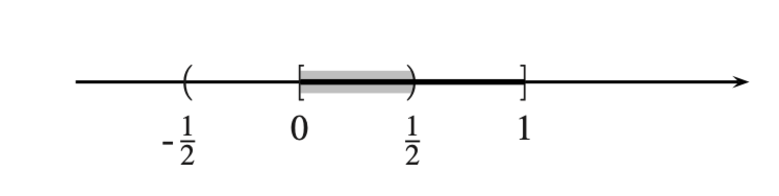
\includegraphics[width=0.5\textwidth]{figures/relative_open}
    \caption{A relatively open set (quoted from
			\cite{tu_introduction_2011})}
		\label{fig:relative_open}
	\end{figure}
\end{example}


%%%%%%%%%%%%%%%%%%%%%%%%%%%%%%%%%%%%%%%%%%%%%%%%%%%%%%%%%%%%%%%%%%%%%%%%%%%%%%%%

\newpage



\section{Bases}

In general, it is fairly difficult to describe all the open sets in a topology
$\mathcal{T}$ explicitly. Usually, however, we can describe a subcollection
$\mathcal{B}$ of $\mathcal{T}$ such that every open set in $\mathcal{T}$ can
be expressed as a union of open sets in $\mathcal{B}$.

\begin{definition}[Basis of a Topology] A subcollection $\mathcal{B}$ of a
	topology $\mathcal{T}$ is a basis for $\mathcal{T}$ if, given any open
	set $U$ and any point $p$ in $U$, there is always an open set
	$B\in\mathcal{B}$ in $\mathcal{B}$ such that $p\in B\subset U$. We also
	say that $\mathcal{B}$ generates the topology $\mathcal{T}$, or that
	$\mathcal{B}$ is a basis for the topological space $S$.

\end{definition}




\begin{example}
	The collection of all open balls $B(p,r)$ in $\mathbb{R}^n$ is a basis
	for the standard topology on $\mathbb{R}^n$, where $p\in\mathbb{R}^n$ is
	any point and $r$ is any positive real number.
\end{example}



\begin{proposition} A collection of open sets $\mathcal{B}$ is a basis for $S$
	if and only if every open set in $S$ can be written as a union of sets in
	$\mathcal{B}$. (The empty set is regarded as the union of zero sets from
	$\mathcal{B}$.)
\end{proposition}

\begin{proof}\quad

	\begin{itemize}
		\item [$\Longrightarrow$] Suppose $\mathcal{B}$ is a basis and $U$ is
		      an arbitrary open set in $S$. For each point $p\in U$, there exists
		      at least one open set $B_p\in \mathcal{B}$ such that $p\in B_p
			      \subset U$. Hence $U=\bigcup_{p\in U}B_p$.

		\item [$\Longleftarrow$] Suppose every open set in $S$ can be written
		      as a union of sets in $\mathcal{B}$. Given an open set $U$ and an
		      arbitrary point $p$ in $U$, since $U$ can be written as a union of
		      sets in $\mathcal{B}$, there must exist a $B_\alpha\in \mathcal{B}$
		      such that $p\in B_\alpha \subset U$. Therefore $\mathcal{B}$ is a
		      basis.
	\end{itemize}
\end{proof}

The following proposition gives a criterion for whether a collection
$\mathcal{B}$ can serve as a basis for some topology.

\begin{proposition}[Criterion for a Basis]
  \label{prop:criterion bases}
	A collection $\mathcal{B}$ of subsets of a set $S$ is a basis for some
	topology $\mathcal{T}$ on $S$ if and only if
	\begin{enumerate}
		\item $S$ is the union of all the sets in $\mathcal{B}$, and
		\item given any two sets $B_1, B_2\in\mathcal{B}$ and any point $p\in
			      B_1\cap B_2$, there exists a set $B\in \mathcal{B}$ such that $p\in
			      B\subset B_1\cap B_2$. See Figure \ref{fig:criterion_bases}.
	\end{enumerate}
\end{proposition}

\begin{figure}[h!]
	\centering
	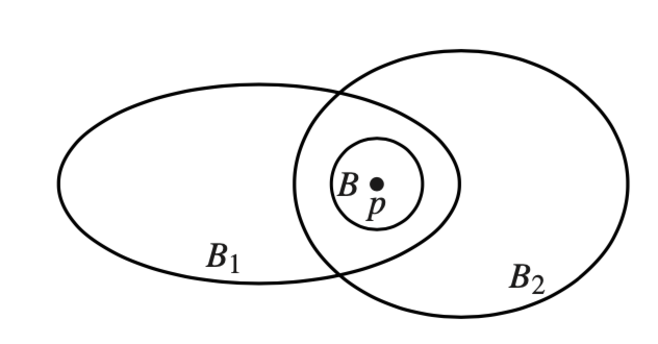
\includegraphics[width=0.5\textwidth]{figures/criterion_bases}
	\caption{The criterion for a basis, from \cite{tu_introduction_2011}}
	\label{fig:criterion_bases}
\end{figure}




\begin{proof}
	($\Longrightarrow$) If the collection $\mathcal{B}$ is a basis for some
	topology $\mathcal{T}$, then of course
	\begin{enumerate}
		\item the whole set $S$ is an open set, and hence can be written as a
		      union of sets in $\mathcal{B}$;
		\item since the sets in $\mathcal{B}$ are all open, for any $B_1, B_2
			      \in\mathcal{B}$ their intersection $B_1\cap B_2$ is also open; if
		      there exists $p\in B_1\cap B_2$, then by the definition of a basis,
		      there exists $B\in\mathcal{B}$ such that $p\in B\subset B_1\cap
			      B_2$.

		      ($\Longleftarrow$) Suppose there is a collection $\mathcal{B}$
		      satisfying conditions 1 and 2. We now construct a collection
		      $\mathcal{T}$ consisting of arbitrary unions of sets in
		      $\mathcal{B}$. We will verify below that $\mathcal{T}$ satisfies
		      all the properties required of a topology.

		      First, $\emptyset$ (the union of zero sets) and $S$ (by condition
		      1) are in $\mathcal{T}$. Second, $\mathcal{T}$ is obviously closed
		      under unions. Finally, it suffices to show that $\mathcal{T}$ is
		      closed under finite intersections. By mathematical induction, it
		      suffices to show that if $U,V\in\mathcal{T}$, then $U\cap
			      V\in\mathcal{T}$. Write $U$ and $V$ as unions of sets in
		      $\mathcal{B}$:
		      \begin{displaymath}
			      U = \bigcup_{\alpha}U_\alpha,\quad V = \bigcup_{\beta} V_\beta
		      \end{displaymath}
		      Then
		      \begin{displaymath}
			      U\cap V = \bigcup_{\alpha,\beta} (U_\alpha \cap V_\beta).
		      \end{displaymath}
		      For any $p\in U\cap V$, there exist some $\alpha$ and $\beta$ such
		      that $p\in U_\alpha\cap V_\beta$. By condition 2, there exists
		      $B_p\in\mathcal{B}$ such that $p\in B_p\subset U_\alpha\cap
			      V_\beta$. Hence
		      \begin{displaymath}
			      U\cap V = \bigcup_{p\in U\cap V} B_p \in\mathcal{T}.
		      \end{displaymath}

	\end{enumerate}
\end{proof}




\begin{proposition}
	Let $\mathcal{B} = \{B_\alpha\}$ be a basis for the topological space
	$S$, and let $A$ be a subspace of $S$. Then $\{B_\alpha\cap A\}$ is a
	basis for $A$.
\end{proposition}


The proof is left to the reader as an exercise.



\subsection{First and Second Countability}

First and second countability, as the names suggest, concern the countability
of bases.


\begin{lemma}
	Every open set in $\mathbb{R}^n$ contains a point all of whose
	coordinates are rational.
\end{lemma}


\begin{proposition}
	The collection $\mathcal{B}_{\text{rat}}$ of all open balls with
	rational centers and rational radii is a basis for $\mathbb{R}^n$.

\end{proposition}

\begin{definition}
	A topological space is said to be \emph{second countable} if it has a
	\underline{countable basis}.
\end{definition}

\begin{definition}
	Let $S$ be a topological space and $p$ a point of $S$. A
	\emph{neighborhood basis} at $p$ is a collection $\mathcal{B} =
		\{B_\alpha\}$ of neighborhoods of $p$ such that for every neighborhood
	$U$ of $p$, there exists a $B_\alpha\in\mathcal{B}$ with $p\in B_\alpha
		\subset U$. A topological space $S$ is said to be \emph{first
		countable} if it has a countable neighborhood basis at every point
	$p\in S$.
\end{definition}

\begin{example}
	For $p\in\mathbb{R}^n$, let $B(p,\frac1n)$ be the open ball centered at
	$p$ with radius $1/n$. Then $\{B(p,\frac1n)\}_{n=1}^\infty$ is a
	neighborhood basis at $p$. Hence $\mathbb{R}^n$ is a first countable
	topological space.
\end{example}


\begin{example}
	An uncountable discrete topological space is first countable but not
	second countable. Every second countable topological space is first
	countable (the proof is left as an exercise).
\end{example}

If $p$ is a point of a first countable topological space and
$\{V_i\}_{i=1}^\infty$ is a countable neighborhood basis at $p$, then setting
$U_i = V_1 \cap \cdots \cap V_i$, we obtain a countable descending sequence
\begin{displaymath}
	U_1 \supset U_2 \supset U_3 \supset \cdots
\end{displaymath}
which is still a neighborhood basis at $p$. Therefore, in giving the
definition of first countability, we may always assume that the countable
neighborhood basis at each point forms a descending sequence of open sets.




\subsection{Exercises} \label{exsec:bases}
\begin{enumerate}

	\item Prove: let $\mathcal{B} = \{B_\alpha\}$ be a basis for the
	      topological space $S$, and let $A$ be a subspace of $S$. Then
	      $\{B_\alpha\cap A\}$ is a basis for $A$.


	\item An uncountable discrete topological space is first countable but not
	      second countable. Every second countable topological space is first
	      countable.
\end{enumerate}

\newpage

\section{Separation Axioms}
There are many formulations of the separation axioms, but in these notes we
need only discuss the Hausdorff separation property and normality.

\begin{definition}[Hausdorff Topological Spaces]
	A topological space $S$ is called a \emph{Hausdorff} space if, given any
	two points $x,y\in S$, there always exist two disjoint open sets $U$ and
	$V$ such that $x\in U$ and $y\in V$. A Hausdorff space is called
	\emph{normal} if, given any two disjoint closed sets $F, G$, there exist
	disjoint open sets $U$, $V$ such that $F\subset U$ and $G\subset V$.

\end{definition}

\begin{figure}[h!]
	\centering
	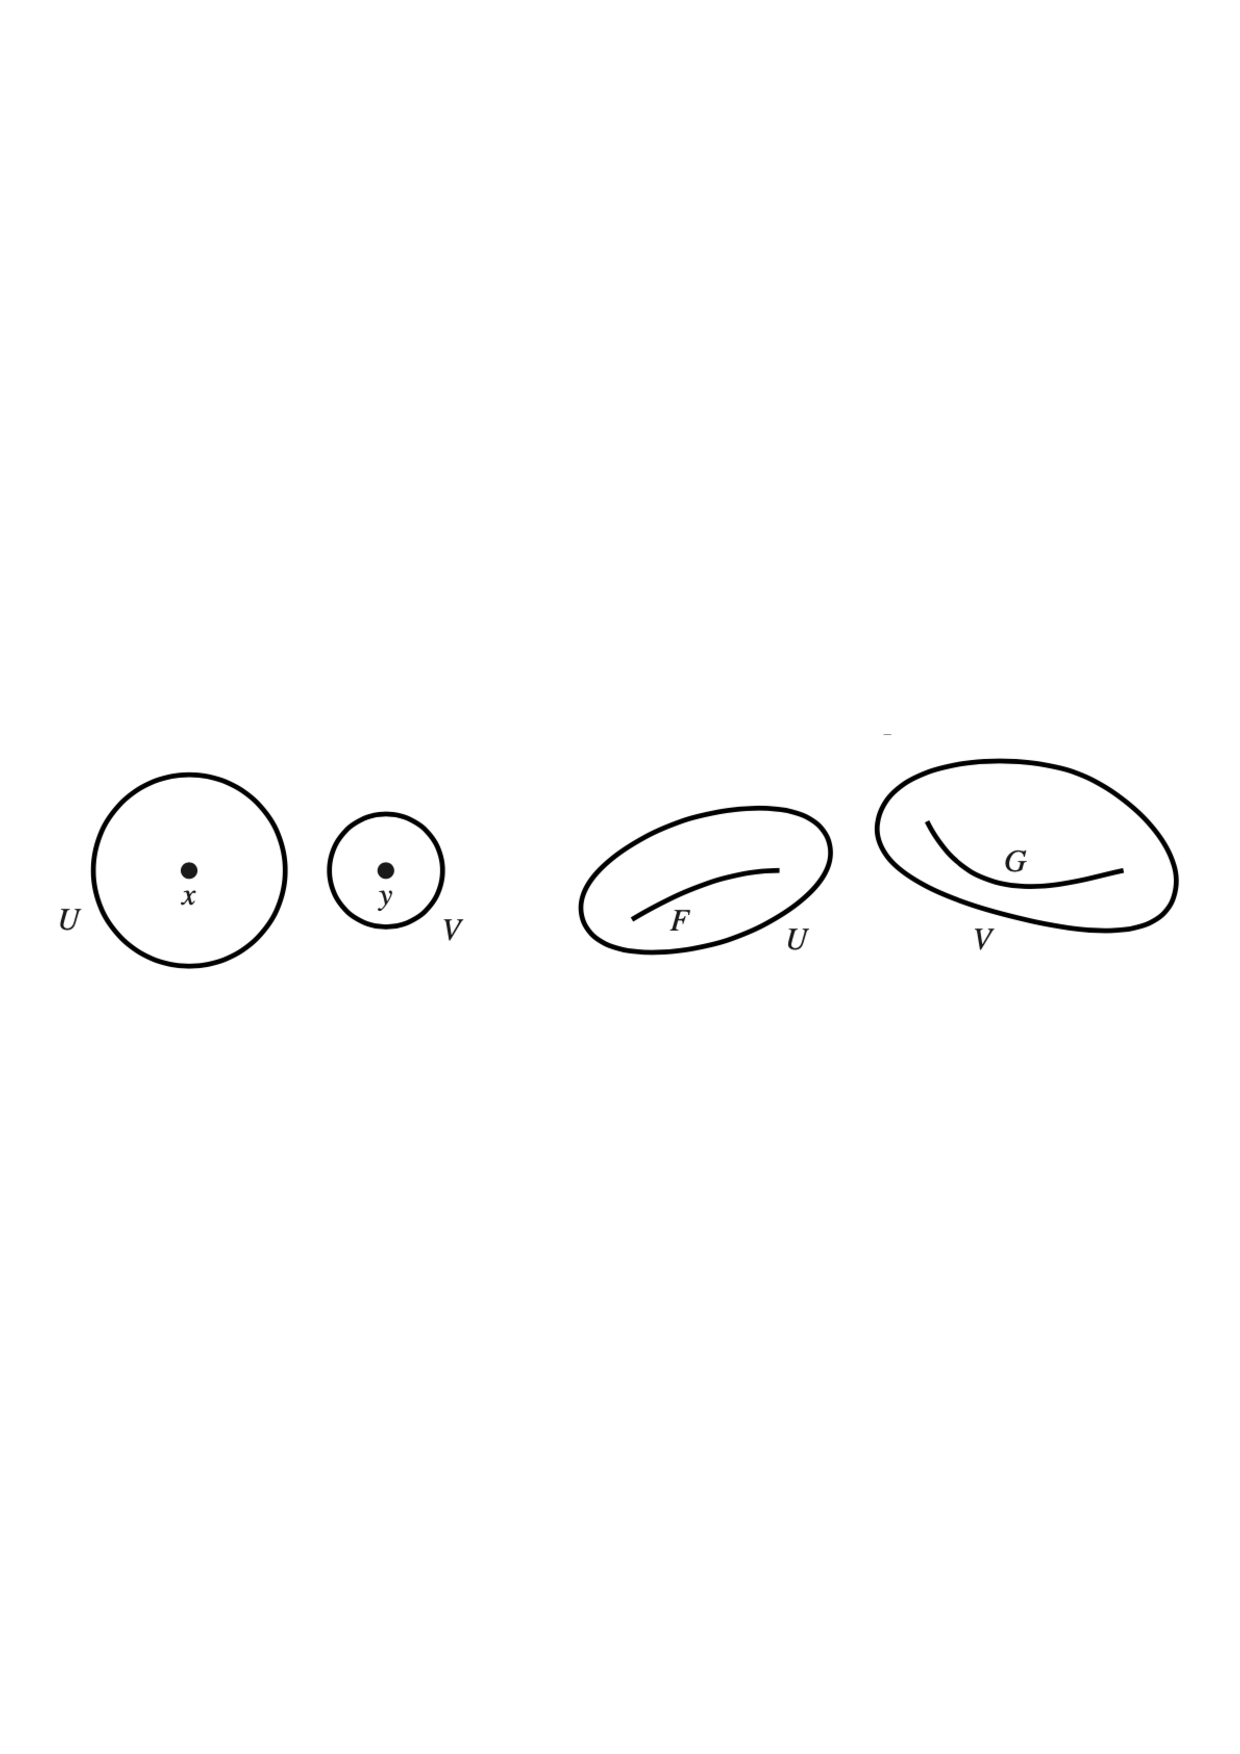
\includegraphics[width=0.5\textwidth]{figures/hausdorff_condition}
	\caption{The Hausdorff condition and normality, from
		\cite{tu_introduction_2011}}
	\label{fig:hausdorff_cond}
\end{figure}



\begin{proposition}
	Every one-point set in a Hausdorff space is closed.
\end{proposition}

The proof is left as an exercise.

\begin{example}[The Euclidean Topology]
	Euclidean space $\mathbb{R}^n$ is a Hausdorff space, because given any
	two distinct points $x,y\in\mathbb{R}^n$, if we take $\epsilon =
		\frac12 d(x,y)$, then the two open balls $B(x,\epsilon)$ and
	$B(y,\epsilon)$ will have no point in common.
\end{example}


\begin{example}[The Zariski Topology]
	Let $S = \mathbb{C}^n$ be the $n$-dimensional vector space over the
	field $\mathbb{C}$, endowed with the Zariski topology. Every open set
	$U$ is of the form $S\smallsetminus Z(I)$, where $I$ is a family of
	polynomials in $n$ variables and $Z(I)$ is the solution set of this
	family. In the Zariski topology, any two nonempty open sets intersect:
	if $U= S\smallsetminus Z(I)$ and $V = S\smallsetminus Z(J)$ are both
	nonempty, then
	\begin{displaymath}
		U\cap V = S\smallsetminus (Z(I)\cup Z(J))
	\end{displaymath}
	is nonempty (since $Z(I) \cup Z(J)$, being the solution set of $I$ or
	$J$, cannot be the whole space). Hence $\mathbb{C}^n$ with the Zariski
	topology is not Hausdorff.
\end{example}


\begin{proposition} Every subspace $A$ of a Hausdorff space $S$ is also
	Hausdorff.

\end{proposition}

The proof is left as an exercise.

\subsection{Exercises} \label{exsec:seperable}

\begin{enumerate}
	\item Prove that every one-point set in a Hausdorff space is closed.
	\item Prove that every subspace $A$ of a Hausdorff space $S$ is also
	      Hausdorff.
\end{enumerate}


\newpage


\section{Product Topology}\label{subsec:product_top}

Given two nonempty sets $A,B$, we can consider the Cartesian product set
$A\times B$, consisting of all ordered pairs $(a,b)$ with $a\in A$, $b\in B$.
Likewise, given two topological spaces $X$ and $Y$, we can consider the
product topological space $X\times Y$, again consisting of all ordered pairs
$(x,y)$ ($x\in X$, $y\in Y$). We only need to define a topology on $X\times
	Y$ that makes it a topological space. We construct the collection
$\mathcal{B}$ consisting of all sets of the form $U\times V$, where $U$ and
$V$ are open sets in $X$ and $Y$ respectively. We call the sets in
$\mathcal{B}$ basic open sets in $X\times Y$.

If $U_1\times V_1$ and $U_2\times V_2$ are both in $\mathcal{B}$, then
\begin{displaymath}
	(U_1\times V_1)\cap (U_2\times V_2) = (U_1\cap U_2)\times (V_1\cap
	V_2)
\end{displaymath}
is also in $\mathcal{B}$. From this we see that $\mathcal{B}$ generates a
topology, called the product topology. Unless otherwise stated, we will always
use this topology on product spaces.


\begin{proposition}
	Let $\{U_i\}$ and $\{V_j\}$ be bases for the topological spaces $X$ and
	$Y$ respectively. Then $\{U_i\times V_j\}$ is a basis for $X\times Y$.
\end{proposition}

The proof is left as an exercise.


\begin{corollary}
	The product of two second countable topological spaces is second
	countable.
\end{corollary}
Clearly; the proof is omitted.


\begin{proposition}
	The product of two Hausdorff topological spaces is Hausdorff.
\end{proposition}

The proof is left as an exercise.

\subsection{Exercises}

\begin{enumerate}
	\item   Let $\{U_i\}$ and $\{V_j\}$ be bases for the topological spaces
	      $X$ and $Y$ respectively. Then $\{U_i\times V_j\}$ is a basis for
	      $X\times Y$.


	\item  The product of two Hausdorff topological spaces is Hausdorff.
\end{enumerate}


\newpage


\section{Compactness}
As in mathematical analysis, we can discuss when a topological space is
compact. Let $S$ be a topological space. A collection of open sets
$\{U_\alpha\}$ in $S$ is called a \emph{cover} (or \emph{open cover}) of $S$
if $S = \bigcup_\alpha U_\alpha$. If a subcollection
$\{U_\alpha\}_{\alpha\in\mathcal{B}\subset\mathcal{A}}$ of
$\{U_\alpha\}_{\alpha\in \mathcal{A}}$ still covers $S$, the subcollection is
called a \emph{subcover} of $S$.

\begin{definition}[Compact Topological Spaces]
	A topological space $S$ is called compact if every open cover of $S$ has
	a finite subcover.
\end{definition}

Via the subspace topology, a subset $A$ of a topological space $S$ is also a
topological space. The subspace $A$ can be covered by open sets of $A$, and
also by open sets of $S$. An open cover of $A$ in $S$ means a collection of
open sets $\{U_\alpha\}$ of $S$ whose union contains $A$. In this sense, $A$
is a compact set in $S$ if and only if every open cover of $A$ in $S$ has a
finite subcover.

\begin{proposition}
	A closed subset of a compact topological space is compact.
\end{proposition}

\begin{proposition}
	A compact subset $K$ of a Hausdorff topological space $S$ and a point
	$p$ outside the set can be separated by open sets; that is, there exist
	an open set $U\supset K$ and an open set $V\ni p$ such that $U\cap
		V=\emptyset$.
\end{proposition}


\begin{proposition}
	Every compact subset $K$ of a Hausdorff space $S$ is closed.
\end{proposition}


\begin{proposition}
	The image of a compact set under a continuous map is compact.
\end{proposition}


\begin{proposition}
	A continuous map from a compact topological space $X$ to a Hausdorff
	space $Y$ is a closed map.
\end{proposition}



\begin{corollary}\label{cor:from-compact-to-hausdorff}
	A continuous bijection $f$ from a compact topological space $X$ to a
	Hausdorff space $Y$ is a homeomorphism.
\end{corollary}



\begin{theorem}[Tychonoff] The product of an arbitrary family of compact
	spaces, endowed with the product topology, is compact.
\end{theorem}

% \section{Boundedness}

\newpage

\section{Connectedness}
\begin{definition}[Connected Topological Spaces]
	A topological space $S$ is called connected if there do not exist two
	nonempty disjoint open subsets $U$ and $V$ such that $S = U\cup V$. A
	subset $A$ of $S$ is called connected if it is connected as a
	topological subspace.
\end{definition}

\begin{proposition}
	A subset $A$ of a topological space $S$ is disconnected if and only if
	there exist open subsets $U$ and $V$ of $S$ such that
	\begin{itemize}
		\item $U\cap A\neq \emptyset$, $V\cap A \neq \emptyset$,
		\item $U\cap V \cap A = \emptyset$,
		\item $A\subset U\cup V$.
	\end{itemize}
	A pair of open sets with the above properties is called a separation of
	$A$.
\end{proposition}

\begin{figure}[h]
	\centering
	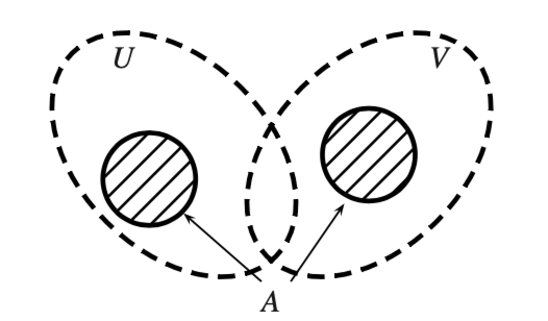
\includegraphics[width=0.5\textwidth]{figures/separation.pdf}
	\caption{A separation of $A$}
\end{figure}

\begin{proposition}
	The image of a connected topological space $X$ under a continuous map
	$f:X\to Y$ is connected.
\end{proposition}

\begin{proof}

\end{proof}

\begin{proposition}
	In a topological space $S$, the union of a family of connected subsets
	$A_\alpha$ having a common point $p$ is connected.
\end{proposition}

\subsection{Connected Components}
Let $x$ be a point of a topological space $S$. The set $C_x$ is the union of
all connected subsets of $S$ containing $x$; it is called the \emph{connected
	component} of $S$ containing $x$.


  \begin{proposition}
	Let $C_x$ be the connected component of a topological space $S$
	containing $x$. Then a connected subset $A\subset S$ is either disjoint
	from $C_x$ or entirely contained in $C_x$.
\end{proposition}

Thus a connected component is a maximal connected subset containing $x$.


\begin{corollary}
	For any two points $x$ and $y$ in a topological space $S$, their
	connected components $C_x$ and $C_y$ are either identical or disjoint.
\end{corollary}

As a consequence of the above corollary, the connected components of $S$
partition $S$ into disjoint subsets.


\newpage

\section{Closure}
Let $S$ be a topological space and $A$ a subset of $S$.

\begin{definition}[Closure]
	The \emph{closure} of $A$ in $S$, denoted $\overline{A}$, or $\cl(A)$,
	or $\cl_S(A)$, is defined as the intersection of all closed sets
	containing $A$.
\end{definition}

It follows from the definition that the closure is necessarily a closed set.
It is the smallest closed set containing $A$ (since every closed set
containing $A$ contains the closure).


\begin{proposition}[Local Characterization of the
	Closure]\label{prop:closure_local}
	Let $A$ be a subset of a topological space $S$. A point $p\in S$ lies in
	the closure $\cl(A)$ if and only if every neighborhood of $p$ contains
	at least one point of $A$.
\end{proposition}

\begin{proof} We will consider the contrapositive of the statement:
	\begin{displaymath}
		p\not\in \cl(A) \Longleftrightarrow \text{there exists a neighborhood
			of $p$ disjoint from $A$}
	\end{displaymath}

	($\Longrightarrow$) Suppose
	\begin{displaymath}
		p\not\in \cl(A) = \bigcap \{F | \text{$F$ is closed in $S$ and
			$F\supset A$}\}.
	\end{displaymath}
	Then $p$ fails to lie in some closed set containing $A$; that is, $p\in
		S\smallsetminus F$, an open set disjoint from $A$.

	($\Longleftarrow$) Suppose $p$ lies in an open set $U$ disjoint from
	$A$. Then the complement $F:=S\smallsetminus U$ is a closed set
	containing $A$ but not $p$. Hence $p\not\in \cl(A)$.

\end{proof}

\begin{example} The closure of the open disk $B(\mathbf{0},r)$ in
	$\mathbb{R}^2$ is the closed disk $\overline{B}(\mathbf{0},r) =
		\{p\in\mathbb{R}^2 \,|\, d(p,\mathbf{0})\le r \}$.

\end{example}

\begin{definition}
	A point $p$ in $S$ is called an \emph{accumulation point} of $A$ if
	every neighborhood of $p$ in $S$ contains a point of $A$ other than $p$.
	The set of all accumulation points of $A$ is denoted $\ac(A)$.
\end{definition}


Let $U$ be a neighborhood of $p$ in $S$; we call $U\smallsetminus\{p\}$ a
\emph{punctured neighborhood} of $p$. Then an equivalent condition for $p$ to
be an accumulation point of $A$ is that every punctured neighborhood of $p$
contains a point of $A$. In some books, an accumulation point is also called a
limit point.

\begin{example}
	If $A=[0,1)\cup\{2\}\subset\mathbb{R}^1$, then the closure of $A$ is
	$[0,1]\cup\{2\}$, but the set of accumulation points of $A$ is the
	closed interval $[0,1]$.
\end{example}

\begin{proposition}
	Let $A$ be a subset of a topological space $S$. Then
	\begin{displaymath}
		\cl(A) = A \cup \ac(A).
	\end{displaymath}
\end{proposition}

\begin{proof}

	($\supset$) By definition, $A\subset \cl(A)$. By the local
	characterization of the closure, $\ac(A)\subset\cl(A)$. Hence $A\cup
		\ac(A) \subset \cl(A)$.

	($\subset$) Let $p\in\cl(A)$. Then either $p\in A$ or $p\not\in A$. If
	$p\in A$, then $p\in A\cup \ac(A)$. Suppose $p\not\in A$. By Proposition
	\ref{prop:closure_local}, every neighborhood of $p$ contains a point of
	$A$ different from $p$ (since $p\not\in A$). Hence every punctured
	neighborhood of $p$ contains a point of $A$. Therefore
	\begin{displaymath}
		p\in \ac(A) \subset A\cup \ac(A).
	\end{displaymath}
	Thus $\cl(A)\subset A\cup \ac(A)$.

\end{proof}

\begin{proposition}
	A set $A$ is closed if and only if $A=\overline{A}$.
\end{proposition}


\begin{proposition}
	If $A\subset B$, then $\overline{A}\subset\overline{B}$.
\end{proposition}


\subsection{Exercises}
\begin{enumerate}
	\item Closures of finite unions and intersections. Let $A$ and $B$ be
	      subsets of a topological space $S$. Prove:
	      \begin{enumerate}
		      \item [(a)] $\overline{A\cup B} = \overline{A} \cup \overline{B}$,
		      \item [(b)] $\overline{A\cap B} \subset \overline{A}\cap
			            \overline{B}$.
	      \end{enumerate}
	      Consider $A=(a,0)$, $B=(0,b)\subset\mathbb{R}$; then in general
	      $\overline{A\cap B} \neq \overline{A} \cap \overline{B}$.

\end{enumerate}


\newpage

\section{Convergence}

Let $S$ be a topological space. A \emph{sequence} in $S$ is a map from
$\mathbb{Z}^+$ to $S$. We denote a sequence by $\{x_i\}$, or by
$x_1,x_2,x_3,\cdots$.

\begin{definition}
	A sequence $\{x_i\}$ converges to a point $p$ if for every neighborhood
	$U$ of $p$, there exists a positive integer $N$ such that $x_i\in U$ for
	all $i\ge N$. In this case we say that $p$ is a limit of the sequence
	$\{x_i\}$, and write $x_i\to p$ or $\lim_{i\to \infty }x_i = p$.
\end{definition}

\begin{proposition}[Uniqueness of Limits]
	In a Hausdorff space $S$, if a sequence $\{x_i\}$ converges both to $p$
	and to $q$, then $p=q$.
\end{proposition}

The proof is left as an exercise.


\begin{proposition}[The Sequence Lemma] Let $S$ be a topological space and
	$A\subset S$. If there exists a sequence $\{a_i\in A\}$ converging to
	$p$, then $p\in\cl(A)$. If $S$ is first countable, the converse is also
	true.

\end{proposition}

\begin{proof}

	($\Longrightarrow$) Suppose $a_i\to p$, where $a_i\in A$. By the
	definition of convergence, every neighborhood of $p$ contains infinitely
	many points of $\{a_i\}$ from some term onward. In particular, $U$
	contains a point of $A$. By Proposition \ref{prop:closure_local},
	$p\in\cl(A)$.

	($\Longleftarrow$) Suppose $p\in\cl(A)$. Since $S$ is first countable,
	we can find a countable neighborhood basis $\{U_n\}$ at $p$ such that
	\begin{displaymath}
		U_1 \supset U_2 \supset \cdots.
	\end{displaymath}
	By the local characterization of the closure, there is an $a_i\in A$ in
	each $U_i$. We claim that the sequence $\{a_i\}$ converges to $p$. If
	$U$ is any neighborhood of $p$, then by the definition of a neighborhood
	basis at $p$, there exists a $U_N$ such that $p\in U_N\subset U$. For
	all $i\ge N$, we have
	\begin{displaymath}
		U_i\subset U_N\subset U.
	\end{displaymath}
	Therefore, for all $i\ge N$,
	\begin{displaymath}
		a_i\in U_i\subset U.
	\end{displaymath}
	This proves that $\{a_i\}$ converges to $p$.


\end{proof}



\subsection{Exercises}
\begin{enumerate}
	\item   In a Hausdorff space $S$, if a sequence $\{x_i\}$ converges both to
	      $p$ and to $q$, then $p=q$.

\end{enumerate}

\newpage


\section{The Quotient Topology}
\label{sec:quotient-topology}

Gluing the edges of a square sheet of rubber along its boundary is a way of
creating new surfaces. For example, gluing together the top and bottom edges
of a square yields a cylinder; gluing the edges of the cylinder with their
orientation preserved yields a \emph{torus} (see Figure
\ref{fig:glue-edge-of-a-square}). Such a gluing operation is called an
\emph{identification} or a \emph{quotient construction}.

\begin{figure}[ht]
	\centering
	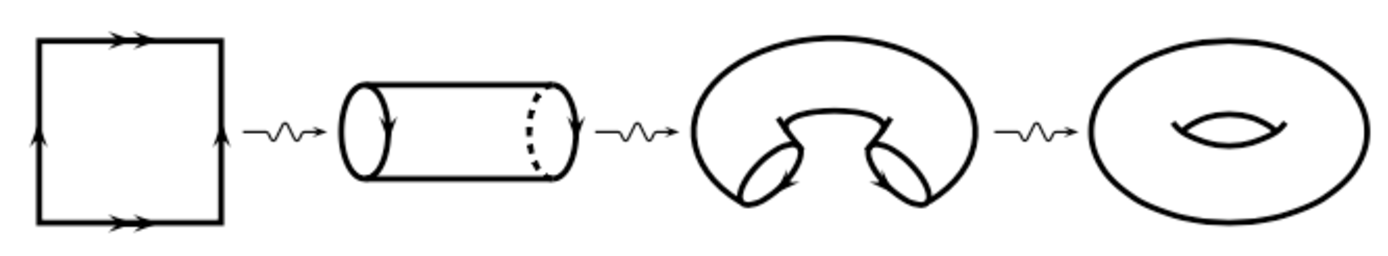
\includegraphics[width=0.8\textwidth]{figures/gluing_edges_of_square}
	\caption{Gluing the edges of a square (figure from
		\cite{tu_introduction_2011})}
	\label{fig:glue-edge-of-a-square}
\end{figure}

A quotient construction is essentially a simplifying operation. Starting from
an equivalence relation on a given set, we regard each equivalence class as a
single point. Mathematics is full of quotient constructions: quotient groups,
quotient rings, quotient spaces, and so on. If the original set is a
topological space, then in general one can always endow the quotient set with
a topology that makes the natural projection map continuous. The main result
of this section is a condition under which the quotient topological space is
still a second countable Hausdorff space.

\subsection{The Quotient Topology}

Recall that an equivalence relation on a set $S$ is reflexive, symmetric, and
transitive. The \emph{equivalence class} $[x]$ of $x\in S$ consists of all
elements of the set equivalent to $x$. An equivalence relation on a set $S$
partitions $S$ into disjoint equivalence classes. We denote the set of
equivalence classes by $S/\sim$ and call it the \emph{quotient} of $S$ under
the equivalence relation $\sim$. The \emph{natural projection map} $\pi: S\to
	S/\sim$ sends $x\in S$ to the equivalence class $[x]$.

Now suppose $S$ is a topological space. We define a topology on $S/\sim$ by
declaring $U\subset S/\sim$ to be \emph{open} if and only if its preimage
$\pi^{-1}(U)$ under the natural projection is open in $S$. Clearly,
$\emptyset$ and the quotient set $S/\sim$ itself are both open. Furthermore,
since
\begin{displaymath}
	\pi^{-1}\left(\bigcup_\alpha U_\alpha\right) = \bigcup_{\alpha}\pi^{-1}(U_\alpha)
\end{displaymath}
and
\begin{displaymath}
	\pi^{-1}\left(\bigcap_i U_i\right) =\bigcap_i \pi^{-1}(U_i),
\end{displaymath}
the collection of all open sets in $S/\sim$ is closed under arbitrary unions
and finite intersections, and hence is a topology. This is called the
\emph{quotient topology} on $S/\sim$. With this topology, $S/\sim$ is called
the \emph{quotient space} of $S$ under the equivalence relation $\sim$. Under
the quotient topology, the projection map $\pi:S\to S/\sim$ is automatically
continuous, since the preimage of an open set is open in $S$ by the very
definition of the quotient topology.


\subsection{Continuity of a Map on a Quotient}

Let $\sim$ be an equivalence relation on a topological space $S$, and let
$S/\sim$ have the quotient topology under this equivalence relation. Suppose a
function $f:S\to Y$ from the topological space $S$ to $Y$ is constant on each
equivalence class. Then it induces a map $\bar{f}: S/\sim \to Y$ given by
\begin{displaymath}
	\bar{f}([p]) = f(p)\quad \text{for $p\in S$}.
\end{displaymath}
In other words, there is a \emph{commutative diagram}
\begin{displaymath}
	\begin{tikzcd}
		S \arrow[r,"f"]\arrow[d,"\pi"] & Y.\\
		S/\sim \arrow[ru,"\bar{f}"]
	\end{tikzcd}
\end{displaymath}

\begin{proposition}
  \label{prop:continuous-of-quotient-map}
	The induced map $\bar{f}: S/\sim\to Y$ is continuous if and only if the
	map $f: S\to Y$ is continuous.
\end{proposition}

\begin{proof}
	\begin{itemize}
		\item [($\Longrightarrow$)] If $\bar{f}$ is continuous, then the
		      composite $\bar{f}\circ \pi$ is continuous, so $f$ is continuous as
		      well.
		\item [($\Longleftarrow$)] Suppose $f$ is continuous. Let $V$ be an
		      open set in $Y$; then $f^{-1}(V)=\pi^{-1}(\bar{f}^{-1}(V))$ is an
		      open set in $S$. By the definition of the quotient topology,
		      $\bar{f}^{-1}(V)$ is open in $S/\sim$. Since $V$ was arbitrary,
		      $\bar{f}: S/\sim\to Y$ is a continuous map.
	\end{itemize}
\end{proof}

This proposition gives a useful criterion for checking whether a map
$\bar{f}$ on the quotient space $S/\sim$ is continuous: simply lift $\bar{f}$
to $f := \bar{f}\circ \pi$ and check whether the lifted map $f$ is continuous
on $S$.


\subsection{Identification of a Subset to a Point}
If $A$ is a subspace of $S$, we define a relation $\sim$ on $S$ by
\begin{displaymath}
	x\sim x \quad \text{for $x\in S$}
\end{displaymath}
and
\begin{displaymath}
	x\sim y \quad \text{for $x,y\in A$}
\end{displaymath}
This is an equivalence relation on $S$. We say that the quotient space
$S/\sim$ is obtained from $S$ by \emph{identifying $A$ to a point}.

\begin{example}
	Let $I$ be the unit interval $[0,1]$, and let $I/\sim$ be the quotient
	space obtained from $I$ by identifying the two points $\{0,1\}$ to a
	single point. Denote the unit circle in the complex plane by $S^1$. Then
	the function $f:I\to S^1$, $f(x)=\exp(2\pi i x)$, takes the same value
	at $0$ and $1$, and hence induces a map $\bar{f}: I/\sim \to S^1$ (see
	Figure \ref{fig:circle-as-quotient-of-interval})

	\begin{figure}[ht]
		\centering
		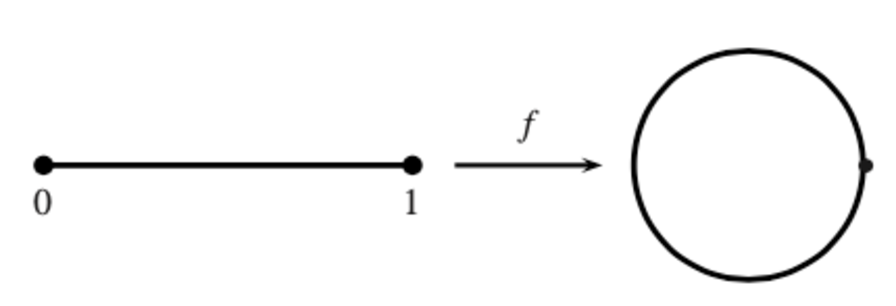
\includegraphics[width=0.6\textwidth]{figures/circle_as_quotient_of_interval}
		\caption{The unit circle as a quotient of the unit interval (figure
			from \cite{tu_introduction_2011})}
		\label{fig:circle-as-quotient-of-interval}
	\end{figure}
\end{example}


\begin{proposition}
  \label{prop:interval-to-s1}
	The map $\bar{f}:I/\sim \to S^1$ is a homeomorphism.
\end{proposition}

\begin{proof}
	Since $f$ is continuous, $\bar{f}$ is also continuous by Proposition
	\ref{prop:continuous-of-quotient-map}. Clearly $\bar{f}$ is a bijection.
	As the image of the compact set $I$ under a continuous map, the quotient
	$I/\sim$ is compact. Hence $\bar{f}$ is a continuous bijection from the
	compact space $I/\sim$ to the Hausdorff space $S^1$, so by Corollary
	\ref{cor:from-compact-to-hausdorff}, $\bar{f}$ is a homeomorphism.
\end{proof}


\subsection{A Necessary Condition for a Hausdorff Quotient}

In general, a quotient construction need not preserve the Hausdorff property
or second countability. In fact, since every one-point set in a Hausdorff
space is closed, if $\pi: S\to S/\sim$ is a projection and the quotient space
$S/\sim$ is Hausdorff, then for every $p\in S$, its image $\{\pi(p)\}$, as a
one-point set in $S/\sim$, should be closed in $S/\sim$. By the continuity of
$\pi$, the preimage $\pi^{-1}(\{\pi(p)\})=[p]$ should be a closed set in $S$.
This gives a necessary condition for a quotient space to be Hausdorff.

\begin{example}
	Define an equivalence relation on $\RR$ by regarding the open interval
	$(0,\infty)$ as a single point. Then the quotient space $R/\sim$ is not
	Hausdorff, because the equivalence class $(0,\infty)$ under $\sim$ is
	not a closed set in $\RR$.
\end{example}


\subsection{Open Equivalence Relations}

In this section we follow the approach of Boothby to derive conditions for a
quotient space to be Hausdorff or second countable. Recall that a map $f:X\to
	Y$ between topological spaces is \emph{open} if the image under $f$ of
every open set is open.

\begin{definition}
	An equivalence relation $\sim$ on a topological space $S$ is called
	\emph{open} if the projection map $\pi: S\to S/\sim$ is an open map.
\end{definition}

In other words, an equivalence relation on $S$ is open if and only if for
every open set $U\subset S$, the set
\begin{displaymath}
	\pi^{-1}(\pi(U)) = \bigcup_{x\in U}[x]
\end{displaymath}
is open.

\begin{figure}[ht]
	\centering
	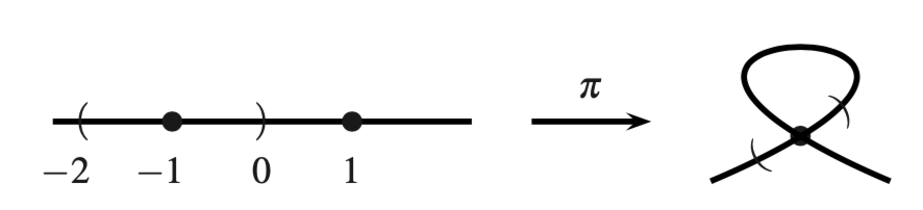
\includegraphics[width=0.6\textwidth]{figures/projection_not_open}
	\caption{A projection map that is not open (figure from
		\cite{tu_introduction_2011})}
	\label{fig:projective-is-not-open}
\end{figure}

\begin{example}

	The projection map onto a quotient space is in general not open. For
	example, let $\sim$ be the equivalence relation on $\RR$ that identifies
	$1$ and $-1$, and let $\pi:\RR\to\RR/\sim$ be the projection map (see
	Figure \ref{fig:projective-is-not-open}).

	The map $\pi$ is open if and only if for every open set
	$V\subset\RR$, its image $\pi(V)$ is open in $\RR/\sim$; by the
	definition of the quotient topology this requires that
	$\pi^{-1}(\pi(V))$ be open in $\RR$. Now take $V=(-2,0)\subset\RR$; then
	\begin{displaymath}
		\pi^{-1}(\pi(V)) = (-2,0)\cup \{1\},
	\end{displaymath}
	which is not an open set in $\RR$. Hence the projection map
	$\pi:\RR\to\RR/\sim$ is not an open map.

\end{example}

Given an equivalence relation $\sim$ on $S$, let $R$ be the subset of $S\times
	S$ defined by
\begin{displaymath}
	R=\{(x,y)\in S\times S\, |\, x\sim y\}.
\end{displaymath}
We call $R$ the \emph{graph} of the equivalence relation $\sim$.


\begin{figure}[ht]
	\centering
	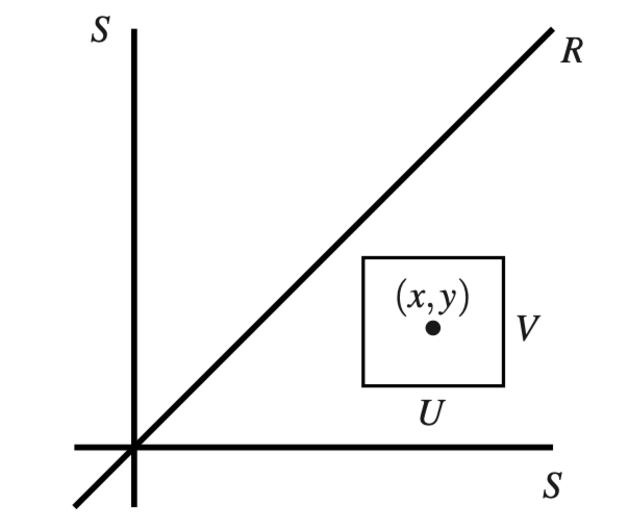
\includegraphics[width=0.4\textwidth]{figures/graph_of_equivalence_relation}
	\caption{The graph $R$ of an equivalence relation and an open set
		$U\times V$ disjoint from $R$ (figure from
		\cite{tu_introduction_2011})}
	\label{fig:graph-of-equivalence-relation}
\end{figure}

\begin{theorem}
  \label{thm:quotient-be-hausdorff}

	Let $\sim$ be an open equivalence relation on a topological space $S$.
	Then the quotient space $S/\sim$ is Hausdorff if and only if the graph
	of the equivalence relation $\sim$ is closed in $S\times S$.

\end{theorem}

\begin{proof}
	We have the following chain of equivalent statements:

	$R$ is closed in $S\times S$

	$\Longleftrightarrow$ $S\times S- R$ is open in $S\times S$

	$\Longleftrightarrow$ for every $(x,y)\in S\times S-R$, there exists a
	basic open set $U\times V$ containing $(x,y)$ such that $(U\times V)\cap
		R = \emptyset$ (see Figure \ref{fig:graph-of-equivalence-relation})

	$\Longleftrightarrow$ for every pair $x\not\sim y$ in $S$, there exist a
	neighborhood $U$ of $x$ and a neighborhood $V$ of $y$ such that no
	element of $U$ is equivalent to any element of $V$

	$\Longleftrightarrow$ for any two points $[x]\neq [y]$ in $S/\sim$,
	there exist a neighborhood $U$ of $x$ and a neighborhood $V$ of $y$ such
	that $\pi(U)\cap \pi(V)=\emptyset$ (in $S/\sim$). \qquad\qquad (*)

	We now show that the last statement (*) is equivalent to $S/\sim$ being
	Hausdorff. First suppose (*) holds. Since $\sim$ is an open equivalence
	relation, $\pi(U)$ and $\pi(V)$ are disjoint open sets in $S/\sim$
	containing $[x]$ and $[y]$ respectively. Hence $S/\sim$ is a Hausdorff
	space.

	Conversely, suppose $S/\sim$ is Hausdorff. Let $[x]\neq [y] \in
		S/\sim$. Then there exist two disjoint open sets $A$ and $B$ in
	$S/\sim$ such that $[x]\in A$, $[y]\in B$. Since the projection map is
	surjective, we have $A=\pi(\pi^{-1} A)$ and $B=\pi(\pi^{-1}B)$. Set
	$U=\pi^{-1}A$ and $V = \pi^{-1}B$. Then $x\in U$, $y\in V$, and
	$A=\pi(U)$, $B=\pi(V)$ are disjoint open sets in $S/\sim$.
\end{proof}

If the equivalence relation $\sim$ is equality, then the quotient space
$S/\sim$ is $S$ itself and the graph $R$ is the diagonal
\begin{displaymath}
	\Delta = \{(x,x)\in S\times S\}.
\end{displaymath}
In this case, Theorem \ref{thm:quotient-be-hausdorff} becomes the following
well-known characterization of Hausdorff spaces in terms of their diagonals.

\begin{corollary}\label{cor:quotient-space-diagonal}
	A topological space $S$ is Hausdorff if and only if its diagonal
	$\Delta\in S\times S$ is closed.
\end{corollary}

\begin{theorem}
	Let $\sim$ be an open equivalence relation on a topological space $S$,
	with projection map $\pi : S\to S/\sim$. If $\mathcal{B} = \{B_\alpha\}$
	is a basis for $S$, then its image $\{\pi(B_\alpha)\}$ is a basis for
	$S/\sim$.
\end{theorem}

\begin{proof}
	Since $\pi$ is an open map, $\{\pi(B_\alpha)\}$ is a collection of open
	sets in $S/\sim$. Let $W$ be an open set in $S/\sim$ with $[x]\in W$,
	$x\in S$. Then $x\in\pi^{-1}(W)$. Since $\pi^{-1}(W)$ is open, there
	exists a basic open set $B\in\mathcal{B}$ such that
	\begin{displaymath}
		x\in B\subset \pi^{-1}(W).
	\end{displaymath}
	Then
	\begin{displaymath}
		[x]=\pi(x)\in\pi(B)\subset W,
	\end{displaymath}
	which proves that $\{\pi(B_\alpha)\}$ is a basis for $S/\sim$.
\end{proof}

\begin{corollary}\label{cor:quotient-second-countable}
	If $\sim$ is an open equivalence relation on a second countable space
	$S$, then the quotient space $S/\sim$ is second countable.
\end{corollary}

\newpage

\chapter{Inverse and Implicit Function Theorems}
\label{sec:inverse-function-theorem}
\noindent\emph{Editorial supplement. This appendix is not part of Warner's original text.}
\medskip

In this chapter we discuss three logically equivalent theorems: the inverse
function theorem, the implicit function theorem, and the constant rank
theorem, which describe the local behavior of $C^\infty$ maps from $\RR^n$ to
$\RR^m$. We assume the inverse function theorem and then derive the other two
theorems from it in the simplest cases.


In subsequent discussions, these theorems are applied on manifolds to study
the local behavior of $C^\infty$ maps, where the maps in question usually have
maximal rank at a point or constant rank in a neighborhood.


\section{The Inverse Function Theorem}

A $C^\infty$ map $f: U\to \RR^n$ defined on an open set $U\subset\RR^n$ is
said to be \emph{locally invertible}, or to be a \emph{local diffeomorphism}
near a point $p\in U$, if $f$ has a $C^\infty$ inverse map in some
neighborhood of $p$. The inverse function theorem gives a criterion for a map
to be locally invertible. We call the matrix $Jf = [\partial f^i/\partial
	x^j]$ the \emph{Jacobian matrix} of $f$, and its determinant $\det
	[\partial f^i/\partial x^j]$ is called the \emph{Jacobian determinant of
	$f$}.

\begin{theorem}[The Inverse Function Theorem]
  \label{thm:inverse-function-theorem-Rn}

	Let $f:U\to\RR^n$ be a $C^\infty$ map defined on an open subset
	$U\subset\RR^n$. At any point $p\in U$, the map $f$ is
	\underline{locally invertible} near $p$ \underline{if and only if} the
	determinant of its Jacobian matrix $\det [\partial f^i/\partial x^j
			(p)]$ is nonzero.

\end{theorem}

% A proof of the theorem can be found in \cite{rudinma}, p. 221, Theorem 9.24.
Note that although the inverse function theorem requires only the Jacobian
determinant at the point $p$ to be nonzero, continuity in fact guarantees
that the Jacobian determinant is nonzero throughout a neighborhood of $p$.


Since the linear map defined by the Jacobian matrix $Jf(p)$ is the best
approximation to $f$ at $p$, it is quite plausible that $f$ being invertible
in a neighborhood of $p$ is equivalent to $Jf(p)$ being invertible (or,
equivalently, to $\det Jf(p)\neq 0$).


\begin{remark}
	Theorem \ref{thm:inverse-function-theorem-Rn} gives a necessary and
	sufficient condition. However, if one only requires the map $f$ to be a
	local homeomorphism (without regard to smoothness), the theorem gives
	only a sufficient condition.
\end{remark}




\section{The Implicit Function Theorem}

As an application of the inverse function theorem, we state the following
implicit function theorem. Let $F:U\subset\RR^m\to\RR^n$ be a $C^\infty$ map,
where $m>n$. If $p\in U$ is a solution of the equation $F(x^1,\cdots,
	x^m)=\bm{0}$, we would like to ask: in some neighborhood of this
solution, do there exist other solutions? If so, how can these solutions be
represented? The implicit function theorem answers these questions in terms of
the rank of the Jacobian matrix of $F$ at $p$.



\begin{theorem}[Implicit Function Theorem]
\label{thm:appendix-implicit}
Let $F$ be a smooth map from an open neighborhood of $(a,b)$ in
$\RR^r\times\RR^n$ to $\RR^n$, with $F(a,b)=0$. If the partial derivative
$D_yF(a,b):\RR^n\to\RR^n$ is invertible, then there are neighborhoods
$A$ of $a$ and $B$ of $b$ and a unique smooth map $g:A\to B$ such that
\[
 F(x,y)=0\quad\Longleftrightarrow\quad y=g(x)
 \qquad((x,y)\in A\times B).
\]
Moreover, $g(a)=b$ and
\[
 Dg(x)=-[D_yF(x,g(x))]^{-1}D_xF(x,g(x)).
\]
\end{theorem}
\begin{proof}
Define $\Phi(x,y)=(x,F(x,y))$. Its derivative at $(a,b)$ is the block matrix
\[
 D\Phi(a,b)=\begin{pmatrix}I&0\\D_xF(a,b)&D_yF(a,b)\end{pmatrix},
\]
which is invertible. By the inverse function theorem, $\Phi$ is a
diffeomorphism between neighborhoods of $(a,b)$ and $(a,0)$. Its inverse
has the form $(u,v)\mapsto(u,h(u,v))$ because $\Phi$ preserves the first
coordinate. Set $g(u)=h(u,0)$ and shrink to product neighborhoods so that
the graph remains in the domain of this inverse. Injectivity of $\Phi$
gives uniqueness and the displayed equivalence. Differentiating
$F(x,g(x))=0$ gives the derivative formula, after shrinking the neighborhoods
so that $D_yF$ remains invertible.
\end{proof}

\begin{corollary}[Regular Level Sets]
If $F:U\subset\RR^m\to\RR^n$ has rank $n$ at $p$ and $F(p)=c$, then
near $p$ the level set $F^{-1}(c)$ is the graph of a smooth function in
$m-n$ variables. In particular, it is a submanifold of dimension $m-n$.
\end{corollary}
\begin{proof}
A nonzero $n\times n$ minor permits a permutation of the variables for
which $D_yF(p)$ is invertible. Apply the implicit function theorem to $F-c$.
\end{proof}

\section{The Constant Rank Theorem}
\begin{theorem}[Constant Rank Theorem]
\label{thm:appendix-constant-rank}
Let $f:U\subset\RR^m\to\RR^n$ be smooth and have constant rank $k$ in
a neighborhood of $p$. There are smooth coordinates centered at $p$ and
$f(p)$ in which $f$ has the form
\[
 (u_1,\ldots,u_m)\longmapsto(u_1,\ldots,u_k,0,\ldots,0).
\]
\end{theorem}
\begin{proof}
For $k=0$, all first derivatives vanish near $p$, so $f$ is constant on a
sufficiently small ball and the assertion follows by translating the target.
For $k>0$, translate $p$ and $f(p)$ to zero and permute the coordinates so
that $\partial(f_1,\ldots,f_k)/\partial(x_1,\ldots,x_k)$ is invertible at
zero. The inverse function theorem applies to
\[
 \Phi(x)=(f_1(x),\ldots,f_k(x),x_{k+1},\ldots,x_m).
\]
In the coordinates $u=\Phi(x)$, the map is
$f\circ\Phi^{-1}(u)=(u_1,\ldots,u_k,h_{k+1}(u),\ldots,h_n(u))$.
Its derivative has the block form
\[
 \begin{pmatrix}I_k&0\\ A&B\end{pmatrix}.
\]
Since its rank is exactly $k$ throughout a neighborhood, $B=0$ there.
On a smaller coordinate box, each $h_j$ therefore depends only on
$u_1,\ldots,u_k$. The target coordinate change
\[
 \Psi(y)=\bigl(y_1,\ldots,y_k,
 y_{k+1}-h_{k+1}(y_1,\ldots,y_k),\ldots,
 y_n-h_n(y_1,\ldots,y_k)\bigr)
\]
has a smooth inverse obtained by adding the same functions. Thus
$\Psi\circ f\circ\Phi^{-1}$ has the asserted form.
\end{proof}

When $k=m$, this is the local form of an immersion; when $k=n$, it is
the local form of a submersion. Unlike the regular-level-set case, a rank
condition at just one point is not sufficient for the general constant-rank
conclusion. For example, $x\mapsto x^2$ has rank zero at zero but is not
locally constant.

\section{Supplementary Linear Algebra}

\subsection{Dual Spaces}\label{sec:dualspace}

If $V$ and $W$ are real linear spaces, we denote by $\Hom(V,W)$ the vector
space of all linear maps $f: V\to W$. The \emph{dual space} $V^\vee$ of $V$ is
defined to be the linear space of all linear real-valued functions on $V$:
\begin{displaymath}
	V^\vee = \Hom(V,\mathbb{R}).
\end{displaymath}
The elements of $V^\vee$ are called \emph{covectors} or $1$-covectors on $V$.

In the discussion below, we always assume that $V$ is a \emph{finite
	dimensional} vector space. Let $e_1,\cdots, e_n$ be a basis of $V$. Then
every vector $v\in V$ can be uniquely expressed as a linear combination $v=
	\sum v^i e_i$, where $v^i\in\mathbb{R}$. Let $\alpha^i: V\to \mathbb{R}$
be the linear function that takes the value of the $i$-th coordinate component
of $v$, $\alpha^i(v) = v^i$. Then
\begin{displaymath}
	\alpha^i(e_j) = \delta^i_j =
	\begin{cases}
		1 & \text{if $i=j$},     \\
		0 & \text{if $i\neq j$}.
	\end{cases}
\end{displaymath}

\begin{proposition}
	The functions $\alpha^1,\cdots, \alpha^n$ form a basis of $V^\vee$.
\end{proposition}

\begin{proof}
For $\lambda\in V^\vee$ and $v=\sum_i v^ie_i$, linearity gives
$\lambda(v)=\sum_i\lambda(e_i)v^i$. Hence
$\lambda=\sum_i\lambda(e_i)\alpha^i$, so the $\alpha^i$ span $V^\vee$.
Evaluating a relation $\sum_i c_i\alpha^i=0$ on each $e_j$ gives $c_j=0$,
which proves linear independence.
\end{proof}


\begin{corollary}
	The dual space $V^\vee$ has the same dimension as the finite dimensional
	vector space $V$.
\end{corollary}

\subsection{Dual Maps and Annihilators}
For a linear map $T:V\to W$, its dual map is
$T^*:W^\vee\to V^\vee$, $T^*(\lambda)=\lambda\circ T$.
For a subspace $E\subset V$, its annihilator is
$E^\circ=\{\lambda\in V^\vee:\lambda|_E=0\}$.
Extending a basis of $E$ to a basis of $V$ shows that
$\dim E^\circ=\dim V-\dim E$.

\begin{proposition}
For finite-dimensional $V$ and $W$,
\[
 \ker T^*=(\operatorname{im}T)^\circ,\qquad
 \operatorname{im}T^*=(\ker T)^\circ.
\]
In particular, $\operatorname{rank}T^*=\operatorname{rank}T$.
\end{proposition}
\begin{proof}
The first equality follows directly from $T^*\lambda=\lambda\circ T$.
Every element of $\operatorname{im}T^*$ vanishes on $\ker T$, giving one
inclusion in the second equality. Conversely, if $\mu$ vanishes on
$\ker T$, the rule $Tv\mapsto\mu(v)$ defines a linear functional on
$\operatorname{im}T$. Extend it to $W$ using a basis; the extension $\lambda$
satisfies $T^*\lambda=\mu$. The rank identity now follows from the
dimension formula for annihilators and rank--nullity.
\end{proof}


\backmatter
\begin{thebibliography}{99}
\addcontentsline{toc}{chapter}{Bibliography}
\small
  \bibitem{1} Bers, L., F. John, and M. Schechter. Partial Differential Equations. New York: John Wiley \& Sons, Inc., 1964.

  \bibitem{2} Bishop, R. L., and R. J. Crittenden. Geometry of Manifolds. New York: Academic Press, 1964.

  \bibitem{3} Bredon, G. E. Sheaf Theory. New York: McGraw-Hill, 1967.

  \bibitem{4} Cartan, H. Séminaire 1950/1951. Paris: Ecole Normale Supérieure, 1955.

  \bibitem{5} Chevalley, C. Theory of Lie Groups I. Princeton, N.J.: Princeton University Press, 1946.

  \bibitem{6} Fleming, W. H. Functions of Several Variables. Reading, Mass.: Addison-Wesley, 1965.

  \bibitem{7} Godement, R. Topologie Algébrique et Théorie des Faisceaux. Paris: Hermann, 1958.

  \bibitem{8} Gunning, R. C. Lectures on Riemann Surfaces. Princeton, N.J.: Princeton University Press, 1966.

  \bibitem{9} Helgason, S. Differential Geometry and Symmetric Spaces. New York: Academic Press, 1962.

  \bibitem{10} Hodge, W. V. D. The Theory and Applications of Harmonic Integrals. 2d ed. Cambridge: Cambridge University Press, 1952.

  \bibitem{11} Hurewicz, W. Lectures on Ordinary Differential Equations. New York and Cambridge, Mass.: John Wiley \& Sons, Inc., and MIT Press, 1958.

  \bibitem{12} Jacobson, N. Lie Algebras. New York: John Wiley \& Sons, Inc., 1962.

  \bibitem{13} Kelley, J. L. General Topology. Princeton, N.J.: Van Nostrand Company, Inc., 1955.

  \bibitem{14} Kervaire, M. A Manifold which does not admit any differentiable structure. Comment. Math. Helv., 35(1961), 1–14.

  \bibitem{15} Kobayashi, S., and K. Nomizu. Foundations of Differential Geometry, vol. 1. New York: John Wiley \& Sons, Inc., 1963.

  \bibitem{16} Kohn, J. J. Introduccion a la teoria de integrales harmonicas. Lecture notes issued by the Centro de Investigacion del IPN, Mexico, 1963.

  \bibitem{17} Lang, S. Introduction to Differentiable Manifolds. New York: John Wiley \& Sons, Inc., 1962.

  \bibitem{18} Loomis, L. H., and S. Sternberg. Advanced Calculus. Reading, Mass.: Addison-Wesley, 1968.

  \bibitem{19} Milnor, J. On manifolds homeomorphic to the 7-sphere. Ann. of Math., 64(1956), 399–405.

  \bibitem{20} Montgomery, D., and L. Zippin. Topological Transformation Groups. New York: Interscience, 1955.

  \bibitem{21} Newns, N., and A. Walker. Tangent planes to a differentiable manifold. J. London Math. Soc., 31(1956), 400–407.

  \bibitem{22} Nirenberg, L. On elliptic partial differential equations. Ann. Scuola Norm. Sup. Pisa, 13(1959), 115–162.

  \bibitem{23} Pontrjagin, L. S. Topological Groups. Princeton, N.J.: Princeton University Press, 1939.

  \bibitem{24} de Rham, G. Variétés Differentiables. Paris: Hermann, 1960.

  \bibitem{25} Samelson, H. Uber die Sphären die als Gruppenräume auftreten. Comment Math. Helv., 13(1940), 144–155.

  \bibitem{26} Singer, I. M., and J. Thorpe. Lecture Notes on Elementary Topology and Geometry. Glenview, Ill.: Scott, Foresman and Company, 1967.

  \bibitem{27} Simmons, G. F. Introduction to Topology and Modern Analysis. New York: McGraw-Hill, 1963.

  \bibitem{28} Spanier, E. H. Algebraic Topology. New York: McGraw-Hill 1966.

  \bibitem{29} Spivak, M. Calculus on Manifolds. New York: W. A. Benjamin, Inc., 1965.

  \bibitem{30} Sternberg, S. Lectures on Differential Geometry. Englewood Cliffs, N.J.: Prentice-Hall, Inc., 1964.

  \bibitem{31} Woll, J. W., Jr. Functions of Several Variables. New York: Harcourt, Brace \& World, Inc., 1966.

  \bibitem{tu_introduction_2011} Tu, L. W. An Introduction to Manifolds. 2nd ed. New York: Springer, 2011.
\end{thebibliography}

% Generated by scripts/build_notation.py; edit notation.json.
\chapter*{Index of Notation}
\markboth{Index of Notation}{}
\addcontentsline{toc}{chapter}{Index of Notation}
Entries are grouped by the discussion in which the notation is introduced
or explained. Item numbers follow Warner; pages and links refer to this reprint.
Some symbols recur with different meanings in different chapters.

{\small\setlength{\tabcolsep}{3pt}\renewcommand{\arraystretch}{1.15}
\begin{longtable}{@{}>{\raggedright\arraybackslash}p{.39\linewidth}>{\raggedright\arraybackslash}p{.39\linewidth}r r@{}}
\toprule Symbol & Meaning & Item & Page\\\midrule\endfirsthead
\toprule Symbol & Meaning & Item & Page\\\midrule\endhead
\bottomrule\endfoot
$\varnothing$ & Empty set & \ref{thm:1.1} & \pageref{thm:1.1} \\
$\mapsto$ & Image of an individual element & \ref{thm:1.1} & \pageref{thm:1.1} \\
$g\circ f$ & Composition of maps & \ref{thm:1.1} & \pageref{thm:1.1} \\
$\mathrm{id}$ & Identity map & \ref{thm:1.1} & \pageref{thm:1.1} \\
$\mathbb{R}^{d},\allowbreak  r_{i}:\mathbb{R}^{d}\to\mathbb{R}$ & Euclidean space and coordinate projections & \ref{thm:1.1} & \pageref{thm:1.1} \\
$\mathbb{C}^{n}$ & Complex Euclidean space & \ref{thm:1.1} & \pageref{thm:1.1} \\
supp $\varphi$ & Support of a function & \ref{thm:1.1} & \pageref{thm:1.1} \\
$\bar{A}$ & Closure of a set & \ref{thm:1.1} & \pageref{thm:1.1} \\
$[\alpha]$ & Total order of a multi-index & \ref{thm:1.1} & \pageref{thm:1.1} \\
$\alpha!$ & Multi-index factorial & \ref{thm:1.1} & \pageref{thm:1.1} \\
$\partial^\alpha/\partial r^\alpha$ & Multi-index partial derivative & \ref{thm:1.1} & \pageref{thm:1.1} \\
$C^{k},\allowbreak  C^{\infty}$ & Differentiability classes & \ref{thm:1.2} & \pageref{thm:1.2} \\
$(U,\allowbreak \varphi),\allowbreak  (U,\allowbreak x_{1},\allowbreak \ldots,\allowbreak x_{d})$ & Coordinate chart and coordinate functions & \ref{thm:1.3} & \pageref{thm:1.3} \\
$(M,\allowbreak \mathcal{F})$ & Manifold with a differentiable structure & \ref{thm:1.4} & \pageref{thm:1.4} \\
$M^{d}$ & A manifold of dimension d & \ref{thm:1.4} & \pageref{thm:1.4} \\
$S^{d}$ & Unit sphere & \ref{thm:1.5} & \pageref{thm:1.5} \\
$Gl(n,\allowbreak \mathbb R)$ & Real general linear group & \ref{thm:1.5} & \pageref{thm:1.5} \\
$C^{\infty}(U),\allowbreak  C^{\infty}(M,\allowbreak N)$ & Smooth functions and smooth maps & \ref{thm:1.6} & \pageref{thm:1.6} \\
$\tilde{F}_{m},\allowbreak  F_{m},\allowbreak  F_{m}^{k}$ & Germs, vanishing germs, and powers of the ideal & \ref{thm:1.13} & \pageref{thm:1.13} \\
$\mathbf{f},\allowbreak  \mathbf{f}(m)$ & Germ of a function and its value & \ref{thm:1.13} & \pageref{thm:1.13} \\
$M_{m}$ & Tangent space at a point & \ref{thm:1.14} & \pageref{thm:1.14} \\
$\mathbf f-\mathbf f(m)$ & Vanishing part of a germ & \ref{thm:1.15} & \pageref{thm:1.15} \\
$\left.\partial/\partial x_i\right|_m,\allowbreak \ \left.\partial f/\partial x_i\right|_m$ & Coordinate tangent vector and partial derivative & \ref{thm:1.19} & \pageref{thm:1.19} \\
$d\varphi,\allowbreak  d\varphi_{m},\allowbreak  \delta\varphi$ & Differential and its dual & \ref{thm:1.22} & \pageref{thm:1.22} \\
$M_{m}^{*}$ & Cotangent space & \ref{thm:1.22} & \pageref{thm:1.22} \\
$\dot{\sigma}(t)$ & Velocity vector of a curve & \ref{thm:1.23} & \pageref{thm:1.23} \\
$T(M),\allowbreak  T^{*}(M)$ & Tangent and cotangent bundles & \ref{thm:1.25} & \pageref{thm:1.25} \\
$^{k}M_{m},\allowbreak  d^{k}f,\allowbreak  M_{m}^{k}$ & Higher order tangent vectors and differentials & \ref{thm:1.26} & \pageref{thm:1.26} \\
$(x-x(m))^{*}$ & Duals of coordinate monomials & \ref{thm:1.26} & \pageref{thm:1.26} \\
$d^{k}\varphi,\allowbreak  \delta^{k}\varphi$ & Higher differentials and their duals & \ref{thm:1.26} & \pageref{thm:1.26} \\
$(M,\allowbreak \psi)$ & Submanifold with its immersion & \ref{thm:1.27} & \pageref{thm:1.27} \\
$i:A\to M$ & Inclusion of a submanifold & \ref{thm:1.38} & \pageref{thm:1.38} \\
$O(d)$ & Orthogonal group & \ref{thm:1.40} & \pageref{thm:1.40} \\
$X_{m},\allowbreak  X_{m}(f),\allowbreak  X(f)$ & Vector field and its action on functions & \ref{thm:1.41} & \pageref{thm:1.41} \\
$[X,\allowbreak Y]$ & Lie bracket of vector fields & \ref{thm:1.44} & \pageref{thm:1.44} \\
$(a(m),\allowbreak b(m))$ & Maximal interval of an integral curve & \ref{thm:1.48} & \pageref{thm:1.48} \\
$X_t,\allowbreak \mathcal D_t$ & Local flow and its domain & \ref{thm:1.48} & \pageref{thm:1.48} \\
$\mathcal D,\allowbreak \ X\in\mathcal D$ & Distribution and a vector field tangent to it & \ref{thm:1.56} & \pageref{thm:1.56} \\
$V\otimes W,\allowbreak  v\otimes w$ & Tensor product and decomposable tensor & \ref{thm:2.1} & \pageref{thm:2.1} \\
$\operatorname{Hom}(V,\allowbreak W)$ & Space of linear maps & \ref{thm:2.2} & \pageref{thm:2.2} \\
$V_{r,\allowbreak s},\allowbreak  T(V)$ & Tensor spaces and tensor algebra & \ref{thm:2.3} & \pageref{thm:2.3} \\
$C(V),\allowbreak  I(V),\allowbreak  I_{k}(V)$ & Tensor subalgebra and alternating relations & \ref{thm:2.4} & \pageref{thm:2.4} \\
$\Lambda(V),\allowbreak  \Lambda_{k}(V)$ & Exterior algebra and its graded pieces & \ref{thm:2.4} & \pageref{thm:2.4} \\
$v\wedge w$ & Exterior product & \ref{thm:2.4} & \pageref{thm:2.4} \\
$\operatorname{sgn}\pi$ & Sign of a permutation & \ref{thm:2.5} & \pageref{thm:2.5} \\
$A_{r}(V)$ & Alternating multilinear forms & \ref{thm:2.5} & \pageref{thm:2.5} \\
$M_{r,\allowbreak s}(V)$ & Multilinear functions on tensor factors & \ref{thm:2.8} & \pageref{thm:2.8} \\
$\langle w_{1}\wedge\cdots\wedge w_{p},\allowbreak v_{1}\wedge\cdots\wedge v_{p}\rangle$ & Pairing of exterior powers & \ref{thm:2.9} & \pageref{thm:2.9} \\
$\varepsilon(u),\allowbreak  i(u)$ & Exterior and interior multiplication & \ref{thm:2.11} & \pageref{thm:2.11} \\
$T_{r,\allowbreak s}(M)$ & Tensor bundle & \ref{thm:2.14} & \pageref{thm:2.14} \\
$\Lambda_{k}^{*}(M),\allowbreak  \Lambda^{*}(M)$ & Bundles of alternating covariant tensors & \ref{thm:2.14} & \pageref{thm:2.14} \\
$E^k(M),\allowbreak E^*(M)$ & Spaces of smooth differential forms & \ref{thm:2.17} & \pageref{thm:2.17} \\
$\omega(X_{1},\allowbreak \ldots,\allowbreak X_{k})$ & Evaluation of a form on vector fields & \ref{thm:2.18} & \pageref{thm:2.18} \\
$\mathfrak{X}(M)$ & Module of smooth vector fields & \ref{thm:2.18} & \pageref{thm:2.18} \\
$d\omega$ & Exterior derivative & \ref{thm:2.20} & \pageref{thm:2.20} \\
$i(X)\omega$ & Interior multiplication by a vector field & \ref{thm:2.21} & \pageref{thm:2.21} \\
$\delta\psi(\omega)$ & Pullback of a differential form & \ref{thm:2.22} & \pageref{thm:2.22} \\
$L_{X}Y$ & Lie derivative of a vector field & \ref{thm:2.24} & \pageref{thm:2.24} \\
$L_{X}\omega$ & Lie derivative of a differential form & \ref{thm:2.24} & \pageref{thm:2.24} \\
$\mathcal I(\mathcal D)$ & Ideal annihilating a distribution & \ref{thm:2.26} & \pageref{thm:2.26} \\
$T^{n}$ & Torus & \ref{thm:3.3} & \pageref{thm:3.3} \\
$l_\sigma,\allowbreak r_\sigma$ & Left and right translations & \ref{thm:3.6} & \pageref{thm:3.6} \\
$V\sigma,\allowbreak \sigma V$ $(\sigma\in G,\allowbreak V\subset G)$ & Right and left translates of a subset & \ref{thm:3.6} & \pageref{thm:3.6} \\
$\mathfrak g$ & Lie algebra of a Lie group & \ref{thm:3.8} & \pageref{thm:3.8} \\
$G_{e}$ & Tangent space at the identity & \ref{thm:3.8} & \pageref{thm:3.8} \\
$\mathfrak{gl}(n,\allowbreak \mathbb R)$ & Real matrix Lie algebra & \ref{thm:3.10} & \pageref{thm:3.10} \\
$x_{ij}(\sigma)$ & Matrix coordinate functions & \ref{thm:3.10} & \pageref{thm:3.10} \\
$\operatorname{End}(V),\allowbreak \operatorname{Aut}(V)$ & Endomorphisms and automorphisms & \ref{thm:3.10} & \pageref{thm:3.10} \\
$\mathfrak{gl}(n,\allowbreak \mathbb C),\allowbreak Gl(n,\allowbreak \mathbb C)$ & Complex matrix algebra and general linear group & \ref{thm:3.10} & \pageref{thm:3.10} \\
$E_{\mathrm{inv}}^p,\allowbreak E_{\mathrm{inv}}^*$ & Left invariant differential forms & \ref{thm:3.11} & \pageref{thm:3.11} \\
$\pi_{1}(X,\allowbreak x_{0})$ & Fundamental group & \ref{thm:3.22} & \pageref{thm:3.22} \\
$\exp_X,\allowbreak \exp$ & Exponential map & \ref{thm:3.30} & \pageref{thm:3.30} \\
$e^{A}$ & Matrix exponential & \ref{thm:3.35} & \pageref{thm:3.35} \\
$A^t,\allowbreak \bar A,\allowbreak A^{-1}$ & Transpose, complex conjugate, and inverse & \ref{thm:3.37} & \pageref{thm:3.37} \\
$U(n),\allowbreak \mathfrak u(n)$ & Unitary group and its Lie algebra & \ref{thm:3.37} & \pageref{thm:3.37} \\
$Sl(n,\allowbreak \mathbb C),\allowbreak \mathfrak{sl}(n,\allowbreak \mathbb C)$ & Complex special linear group and its Lie algebra & \ref{thm:3.37} & \pageref{thm:3.37} \\
$O(n,\allowbreak \mathbb C),\allowbreak \mathfrak o(n,\allowbreak \mathbb C)$ & Complex orthogonal group and its Lie algebra & \ref{thm:3.37} & \pageref{thm:3.37} \\
$SU(n),\allowbreak \mathfrak{su}(n)$ & Special unitary group and its Lie algebra & \ref{thm:3.37} & \pageref{thm:3.37} \\
$Sl(n,\allowbreak \mathbb R),\allowbreak \mathfrak{sl}(n,\allowbreak \mathbb R)$ & Real special linear group and its Lie algebra & \ref{thm:3.37} & \pageref{thm:3.37} \\
$O(n),\allowbreak \mathfrak o(n),\allowbreak SO(n)$ & Orthogonal groups and their Lie algebra & \ref{thm:3.37} & \pageref{thm:3.37} \\
$\operatorname{Ad}$ & Adjoint representation of a group & \ref{thm:3.46} & \pageref{thm:3.46} \\
$\operatorname{ad}$ & Adjoint representation of a Lie algebra & \ref{thm:3.46} & \pageref{thm:3.46} \\
$G/H$ & Homogeneous quotient manifold & \ref{thm:3.58} & \pageref{thm:3.58} \\
$P^{n},\allowbreak CP^{n}$ & Real and complex projective spaces & \ref{thm:3.65} & \pageref{thm:3.65} \\
$S_{p}(V),\allowbreak M_{k}(V)$ & Stiefel and Grassmann manifolds & \ref{thm:3.65} & \pageref{thm:3.65} \\
$J_\varphi$ & Jacobian determinant & \ref{thm:4.4} & \pageref{thm:4.4} \\
$\Delta^{p}$ & Standard simplex & \ref{thm:4.6} & \pageref{thm:4.6} \\
$k_{i}^{p},\allowbreak \sigma^{i},\allowbreak \partial\sigma$ & Face inclusions, faces, and boundary & \ref{thm:4.6} & \pageref{thm:4.6} \\
$\int_\sigma\omega$ & Integral of a form over a simplex & \ref{thm:4.6} & \pageref{thm:4.6} \\
$\int_{D}\omega$ & Integral over a regular domain & \ref{thm:4.8} & \pageref{thm:4.8} \\
$\langle\ ,\allowbreak \ \rangle_{m}$ & Riemannian inner product at a point & \ref{thm:4.10} & \pageref{thm:4.10} \\
$\operatorname{grad}f,\allowbreak \operatorname{div}V$ & Gradient and divergence & \ref{thm:4.10} & \pageref{thm:4.10} \\
$H_{\mathrm{de\,\allowbreak R}}^p(M)$ & de Rham cohomology & \ref{thm:4.13} & \pageref{thm:4.13} \\
${}_\infty S_p(M,\allowbreak \mathbb R),\allowbreak {}_\infty H_p(M;\mathbb R)$ & Differentiable singular chains and homology & \ref{thm:4.16} & \pageref{thm:4.16} \\
$K,\allowbreak \mathbb Z$ & Coefficient ring and the integers & \ref{thm:5.1} & \pageref{thm:5.1} \\
$\mathcal S,\allowbreak \mathcal S_m$ & Sheaf and its stalk & \ref{thm:5.1} & \pageref{thm:5.1} \\
$\mathcal S\circ\mathcal S$ & Pairs of sheaf elements in the same stalk & \ref{thm:5.1} & \pageref{thm:5.1} \\
$\Gamma(\mathcal S,\allowbreak U),\allowbreak \Gamma(\mathcal S)$ & Local and global sections of a sheaf & \ref{thm:5.1} & \pageref{thm:5.1} \\
$\mathcal C^\infty(M),\allowbreak \mathcal C^p(M)$ & Sheaves of germs of differentiable functions & \ref{thm:5.2} & \pageref{thm:5.2} \\
$P=\{S_{U};\rho_{U,\allowbreak V}\}$ & Presheaf and its restriction maps & \ref{thm:5.5} & \pageref{thm:5.5} \\
$\alpha(\mathcal S)$ & Presheaf associated with a sheaf & \ref{thm:5.6} & \pageref{thm:5.6} \\
$\beta(P)$ & Sheaf associated with a presheaf & \ref{thm:5.6} & \pageref{thm:5.6} \\
$\mathcal S\otimes\mathcal T$ & Tensor product of sheaves & \ref{thm:5.9} & \pageref{thm:5.9} \\
$C^{*}$ & Cochain complex & \ref{thm:5.16} & \pageref{thm:5.16} \\
$d^{q}\colon C^{q}\to C^{q+1}$ & Cochain differential & \ref{thm:5.16} & \pageref{thm:5.16} \\
$Z^{q}(C^{*}),\allowbreak B^{q}(C^{*}),\allowbreak H^{q}(C^{*})$ & Cocycles, coboundaries, and cohomology & \ref{thm:5.16} & \pageref{thm:5.16} \\
$C^{\ast}\to D^{\ast}$ & Cochain map & \ref{thm:5.16} & \pageref{thm:5.16} \\
$\partial$ & Connecting homomorphism & \ref{thm:5.17} & \pageref{thm:5.17} \\
$\mathcal{H},\allowbreak H^{q}(M,\allowbreak \mathcal{S})$ & Sheaf cohomology theory and its groups & \ref{thm:5.18} & \pageref{thm:5.18} \\
$\Gamma(\mathcal{C}^{\ast}\otimes\mathcal{S})$ & Global sections of a tensor resolution & \ref{thm:5.20} & \pageref{thm:5.20} \\
$\mathcal S_0$ & Sheaf of germs of discontinuous sections & \ref{thm:5.22} & \pageref{thm:5.22} \\
$U^{p+1},\allowbreak A^{p}(U,\allowbreak K)$ & Cartesian power and Alexander--Spanier cochains & \ref{thm:5.26} & \pageref{thm:5.26} \\
$d:A^{p}(U,\allowbreak K)\to A^{p+1}(U,\allowbreak K)$ & Alexander--Spanier differential & \ref{thm:5.26} & \pageref{thm:5.26} \\
$A^{*}(U,\allowbreak K),\allowbreak \mathcal{A}^{p}(M,\allowbreak K)$ & Alexander--Spanier complex and associated sheaves & \ref{thm:5.26} & \pageref{thm:5.26} \\
$\mathcal{A}^{*}(M,\allowbreak K),\allowbreak A^{p}(U,\allowbreak G),\allowbreak A_{0}^{p}(U,\allowbreak G)$ & Coefficient variants and locally zero cochains & \ref{thm:5.26} & \pageref{thm:5.26} \\
$H_{A-S}^{q}(M;G)$ & Alexander--Spanier cohomology & \ref{thm:5.26} & \pageref{thm:5.26} \\
$\mathcal{E}^{p}(M)$ & Sheaf of germs of differential forms & \ref{thm:5.28} & \pageref{thm:5.28} \\
$\mathcal{E}^{*}(M)$ & de Rham complex of sheaves & \ref{thm:5.28} & \pageref{thm:5.28} \\
$E^{*}(M)$ & Complex of global differential forms & \ref{thm:5.30} & \pageref{thm:5.30} \\
$S_{p}(U),\allowbreak S^{p}(U,\allowbreak K),\allowbreak S_{0}^{p}(U,\allowbreak K)$ & Singular chains and cochains & \ref{thm:5.31} & \pageref{thm:5.31} \\
$d:S^{p}(U,\allowbreak K)\to S^{p+1}(U,\allowbreak K)$ & Singular coboundary map & \ref{thm:5.31} & \pageref{thm:5.31} \\
$S^{*}(U,\allowbreak K),\allowbreak S^{p}(M,\allowbreak K),\allowbreak S_{0}^{p}(M,\allowbreak K)$ & Singular cochain complexes & \ref{thm:5.31} & \pageref{thm:5.31} \\
$S^{p}(U,\allowbreak G)$ & Singular cochains with module coefficients & \ref{thm:5.32} & \pageref{thm:5.32} \\
$H_\Delta^q(M;G),\allowbreak H_{\Delta^\infty}^q(M;G)$ & Continuous and differentiable singular cohomology & \ref{thm:5.32} & \pageref{thm:5.32} \\
$S_{\mathfrak U}^q(M,\allowbreak G)$ & Cochains on simplices subordinate to a cover & \ref{thm:5.32} & \pageref{thm:5.32} \\
$C^q(\mathfrak U,\allowbreak \mathcal S)$ & Čech cochains of an open cover & \ref{thm:5.33} & \pageref{thm:5.33} \\
$d:C^q\to C^{q+1}$ & Čech coboundary map & \ref{thm:5.33} & \pageref{thm:5.33} \\
$\check H^q(\mathfrak U,\allowbreak \mathcal S)$ & Čech cohomology of a cover & \ref{thm:5.33} & \pageref{thm:5.33} \\
$\check H^q(M,\allowbreak \mathcal S),\allowbreak \check H^q(M;G)$ & Čech cohomology of a space & \ref{thm:5.33} & \pageref{thm:5.33} \\
$C^*\otimes {}^{\prime}C^*$ & Tensor product of cochain complexes & \ref{thm:5.39} & \pageref{thm:5.39} \\
$\mathcal S\oplus\mathcal T$ & Direct sum of sheaves & \ref{thm:5.41} & \pageref{thm:5.41} \\
$f\smile g$ & Cup product of singular cochains & \ref{thm:5.44} & \pageref{thm:5.44} \\
$\Delta g$ & Laplace--Beltrami operator & \ref{thm:6.1} & \pageref{thm:6.1} \\
$\ast:\Lambda_p\to\Lambda_{n-p}$ & Hodge star operator & \ref{thm:6.1} & \pageref{thm:6.1} \\
$\delta$ & Codifferential & \ref{thm:6.1} & \pageref{thm:6.1} \\
$H^p$ & Harmonic p-forms & \ref{thm:6.7} & \pageref{thm:6.7} \\
$(H^p)^\perp$ & Orthogonal complement of harmonic forms & \ref{thm:6.8} & \pageref{thm:6.8} \\
$H,\allowbreak G$ & Harmonic projection and Green operator & \ref{thm:6.9} & \pageref{thm:6.9} \\
$H_p(M;\mathbb R)$ & Real singular homology & \ref{thm:6.14} & \pageref{thm:6.14} \\
$D^\alpha,\allowbreak \mathcal P$ & Differential multi-index notation and periodic functions & \ref{thm:6.15} & \pageref{thm:6.15} \\
$\eta^\alpha$ & Multi-index power & \ref{thm:6.15} & \pageref{thm:6.15} \\
$\varphi\cdot\psi$ & Pointwise Hermitian product & \ref{thm:6.15} & \pageref{thm:6.15} \\
$|\psi|,\allowbreak \|\psi\|$ & Pointwise norm and normalized L2 norm & \ref{thm:6.15} & \pageref{thm:6.15} \\
$\langle\psi,\allowbreak \varphi\rangle$ & Normalized L2 inner product & \ref{thm:6.15} & \pageref{thm:6.15} \\
$\|\psi\|_\infty$ & Uniform norm & \ref{thm:6.15} & \pageref{thm:6.15} \\
$\varphi_\xi$ & Fourier coefficient & \ref{thm:6.16} & \pageref{thm:6.16} \\
$H_s,\allowbreak \|u\|_s$ & Sobolev spaces and norms & \ref{thm:6.17} & \pageref{thm:6.17} \\
$\langle u,\allowbreak v\rangle_s$ & Sobolev inner product & \ref{thm:6.17} & \pageref{thm:6.17} \\
$K^t$ & Sobolev order-shifting Fourier multiplier & \ref{thm:6.17} & \pageref{thm:6.17} \\
$u^h$ & Difference quotient & \ref{thm:6.19} & \pageref{thm:6.19} \\
$T_h$ & Translation by h & \ref{thm:6.19} & \pageref{thm:6.19} \\
$L=\{L_{ij}\},\allowbreak L^*$ & Differential operator and formal adjoint & \ref{thm:6.24} & \pageref{thm:6.24} \\
$\sigma_L$ & Principal symbol of a differential operator & \ref{thm:6.28} & \pageref{thm:6.28} \\
$C^\infty,\allowbreak C_0^\infty,\allowbreak C_0^\infty(V)$ & Smooth and compactly supported test functions & \ref{thm:6.31} & \pageref{thm:6.31} \\
\end{longtable}}



\clearpage
\phantomsection
\addcontentsline{toc}{chapter}{\indexname}
\printindex

\end{document}
